\documentclass[a4paper]{book}
\usepackage{makeidx}
\usepackage{graphicx}
\usepackage{multicol}
\usepackage{float}
\usepackage{listings}
\usepackage{color}
\usepackage{textcomp}
\usepackage{alltt}
\usepackage{times}
\usepackage{ifpdf}
\ifpdf
\usepackage[pdftex,
            pagebackref=true,
            colorlinks=true,
            linkcolor=blue,
            unicode
           ]{hyperref}
\else
\usepackage[ps2pdf,
            pagebackref=true,
            colorlinks=true,
            linkcolor=blue,
            unicode
           ]{hyperref}
\usepackage{pspicture}
\fi
\usepackage[utf8]{inputenc}
\usepackage{doxygen}
\lstset{language=C++,inputencoding=utf8,basicstyle=\footnotesize,breaklines=true,breakatwhitespace=true,tabsize=4,numbers=left }
\makeindex
\setcounter{tocdepth}{3}
\renewcommand{\footrulewidth}{0.4pt}
\begin{document}
\hypersetup{pageanchor=false}
\begin{titlepage}
\vspace*{7cm}
\begin{center}
{\Large ToolDAQFramework }\\
\vspace*{1cm}
{\large Generated by Doxygen 1.6.1}\\
\vspace*{0.5cm}
{\small Wed Aug 28 15:53:21 2019}\\
\end{center}
\end{titlepage}
\clearemptydoublepage
\pagenumbering{roman}
\tableofcontents
\clearemptydoublepage
\pagenumbering{arabic}
\hypersetup{pageanchor=true}
\chapter{Class Index}
\section{Class Hierarchy}
This inheritance list is sorted roughly, but not completely, alphabetically\-:\begin{DoxyCompactList}
\item \contentsline{section}{A\-N\-N\-I\-E\-Geometry}{\pageref{classANNIEGeometry}}{}
\item \contentsline{section}{A\-N\-N\-I\-E\-Reco\-Object\-Table}{\pageref{classANNIERecoObjectTable}}{}
\item \contentsline{section}{Card\-Data}{\pageref{classCardData}}{}
\item \contentsline{section}{Data\-Model}{\pageref{classDataModel}}{}
\item \contentsline{section}{Example\-Root}{\pageref{classExampleRoot}}{}
\item \contentsline{section}{Fo\-M\-Calculator}{\pageref{classFoMCalculator}}{}
\item \contentsline{section}{annie\-:\-:Hefty\-Tree\-Reader}{\pageref{classannie_1_1HeftyTreeReader}}{}
\item \contentsline{section}{I\-F\-Beam\-D\-B\-Interface}{\pageref{classIFBeamDBInterface}}{}
\item \contentsline{section}{L\-A\-P\-P\-D}{\pageref{classLAPPD}}{}
\item \contentsline{section}{L\-A\-P\-P\-Dresponse}{\pageref{classLAPPDresponse}}{}
\item \contentsline{section}{L\-A\-P\-P\-D\-Tree}{\pageref{classLAPPDTree}}{}
\item \contentsline{section}{Minuit\-Optimizer}{\pageref{classMinuitOptimizer}}{}
\item \contentsline{section}{M\-R\-D\-Tree}{\pageref{classMRDTree}}{}
\item \contentsline{section}{N\-C\-V\-Position\-Info}{\pageref{structNCVPositionInfo}}{}
\item \contentsline{section}{Parameters}{\pageref{classParameters}}{}
\item \contentsline{section}{P\-M\-T\-Data}{\pageref{classPMTData}}{}
\item \contentsline{section}{quaternion}{\pageref{structquaternion}}{}
\item \contentsline{section}{annie\-:\-:Raw\-Analyzer}{\pageref{classannie_1_1RawAnalyzer}}{}
\item \contentsline{section}{annie\-:\-:Raw\-Card}{\pageref{classannie_1_1RawCard}}{}
\item \contentsline{section}{annie\-:\-:Raw\-Channel}{\pageref{classannie_1_1RawChannel}}{}
\item \contentsline{section}{annie\-:\-:Raw\-Reader}{\pageref{classannie_1_1RawReader}}{}
\item \contentsline{section}{annie\-:\-:Raw\-Readout}{\pageref{classannie_1_1RawReadout}}{}
\item \contentsline{section}{annie\-:\-:Raw\-Trig\-Data}{\pageref{classannie_1_1RawTrigData}}{}
\item \contentsline{section}{annie\-:\-:Reco\-Pulse}{\pageref{classannie_1_1RecoPulse}}{}
\item \contentsline{section}{annie\-:\-:Reco\-Readout}{\pageref{classannie_1_1RecoReadout}}{}
\item Serialisable\-Object\begin{DoxyCompactList}
\item \contentsline{section}{Beam\-Data\-Point}{\pageref{structBeamDataPoint}}{}
\item \contentsline{section}{Beam\-Status}{\pageref{classBeamStatus}}{}
\item \contentsline{section}{Beam\-Status\-Class}{\pageref{classBeamStatusClass}}{}
\item \contentsline{section}{Channel}{\pageref{classChannel}}{}
\item \contentsline{section}{Channel\-Key}{\pageref{classChannelKey}}{}
\item \contentsline{section}{Detector}{\pageref{classDetector}}{}
\item \contentsline{section}{Direction}{\pageref{classDirection}}{}
\item \contentsline{section}{Geometry}{\pageref{classGeometry}}{}
\item \contentsline{section}{Hefty\-Info}{\pageref{classHeftyInfo}}{}
\item \contentsline{section}{Hit}{\pageref{classHit}}{}
\begin{DoxyCompactList}
\item \contentsline{section}{A\-D\-C\-Pulse}{\pageref{classADCPulse}}{}
\item \contentsline{section}{L\-A\-P\-P\-D\-Hit}{\pageref{classLAPPDHit}}{}
\begin{DoxyCompactList}
\item \contentsline{section}{M\-C\-L\-A\-P\-P\-D\-Hit}{\pageref{classMCLAPPDHit}}{}
\end{DoxyCompactList}
\item \contentsline{section}{L\-A\-P\-P\-D\-Pulse}{\pageref{classLAPPDPulse}}{}
\item \contentsline{section}{M\-C\-Hit}{\pageref{classMCHit}}{}
\end{DoxyCompactList}
\item \contentsline{section}{M\-R\-D\-Out}{\pageref{classMRDOut}}{}
\item \contentsline{section}{Particle}{\pageref{classParticle}}{}
\begin{DoxyCompactList}
\item \contentsline{section}{M\-C\-Particle}{\pageref{classMCParticle}}{}
\end{DoxyCompactList}
\item \contentsline{section}{Position}{\pageref{classPosition}}{}
\item \contentsline{section}{Reco\-Cluster}{\pageref{classRecoCluster}}{}
\item \contentsline{section}{Reco\-Cluster\-Digit}{\pageref{classRecoClusterDigit}}{}
\item \contentsline{section}{Reco\-Digit}{\pageref{classRecoDigit}}{}
\item \contentsline{section}{Reco\-Ring}{\pageref{classRecoRing}}{}
\item \contentsline{section}{Reco\-Vertex}{\pageref{classRecoVertex}}{}
\item \contentsline{section}{Time\-Class}{\pageref{classTimeClass}}{}
\item \contentsline{section}{Trigger\-Class}{\pageref{classTriggerClass}}{}
\item \contentsline{section}{Waveform$<$ T $>$}{\pageref{classWaveform}}{}
\begin{DoxyCompactList}
\item \contentsline{section}{Calibrated\-A\-D\-C\-Waveform$<$ T $>$}{\pageref{classCalibratedADCWaveform}}{}
\end{DoxyCompactList}
\end{DoxyCompactList}
\item \contentsline{section}{T\-Banded\-L\-E}{\pageref{classTBandedLE}}{}
\item T\-Named\begin{DoxyCompactList}
\item \contentsline{section}{T\-One\-Pad\-Display}{\pageref{classTOnePadDisplay}}{}
\item \contentsline{section}{T\-Spline\-Fit}{\pageref{classTSplineFit}}{}
\end{DoxyCompactList}
\item Tool\begin{DoxyCompactList}
\item \contentsline{section}{A\-D\-C\-Calibrator}{\pageref{classADCCalibrator}}{}
\item \contentsline{section}{A\-D\-C\-Hit\-Finder}{\pageref{classADCHitFinder}}{}
\item \contentsline{section}{Beam\-Checker}{\pageref{classBeamChecker}}{}
\item \contentsline{section}{Beam\-Fetcher}{\pageref{classBeamFetcher}}{}
\item \contentsline{section}{Beam\-Time\-Ana}{\pageref{classBeamTimeAna}}{}
\item \contentsline{section}{Beam\-Time\-Tree\-Maker}{\pageref{classBeamTimeTreeMaker}}{}
\item \contentsline{section}{Beam\-Time\-Tree\-Reader}{\pageref{classBeamTimeTreeReader}}{}
\item \contentsline{section}{Check\-Detector\-Counts}{\pageref{classCheckDetectorCounts}}{}
\item \contentsline{section}{Digit\-Builder}{\pageref{classDigitBuilder}}{}
\item \contentsline{section}{Digit\-Builder\-Do\-E}{\pageref{classDigitBuilderDoE}}{}
\item \contentsline{section}{Digit\-Builder\-R\-O\-O\-T}{\pageref{classDigitBuilderROOT}}{}
\item \contentsline{section}{Dummy\-Tool}{\pageref{classDummyTool}}{}
\item \contentsline{section}{Event\-Display}{\pageref{classEventDisplay}}{}
\item \contentsline{section}{Event\-Selector}{\pageref{classEventSelector}}{}
\item \contentsline{section}{Event\-Selector\-Do\-E}{\pageref{classEventSelectorDoE}}{}
\item \contentsline{section}{Example\-Generate\-Data}{\pageref{classExampleGenerateData}}{}
\item \contentsline{section}{Example\-Load\-Root}{\pageref{classExampleLoadRoot}}{}
\item \contentsline{section}{Exampleload\-Store}{\pageref{classExampleloadStore}}{}
\item \contentsline{section}{Example\-Over\-Tool}{\pageref{classExampleOverTool}}{}
\item \contentsline{section}{Example\-Print\-Data}{\pageref{classExamplePrintData}}{}
\item \contentsline{section}{Example\-Save\-Root}{\pageref{classExampleSaveRoot}}{}
\item \contentsline{section}{Example\-Save\-Store}{\pageref{classExampleSaveStore}}{}
\item \contentsline{section}{Find\-Mrd\-Tracks}{\pageref{classFindMrdTracks}}{}
\item \contentsline{section}{Find\-Track\-Length\-In\-Water}{\pageref{classFindTrackLengthInWater}}{}
\item \contentsline{section}{Generate\-Hits}{\pageref{classGenerateHits}}{}
\item \contentsline{section}{Histograms\-Root\-L\-A\-P\-P\-D\-Data}{\pageref{classHistogramsRootLAPPDData}}{}
\item \contentsline{section}{Hit\-Cleaner}{\pageref{classHitCleaner}}{}
\item \contentsline{section}{Hit\-Residuals}{\pageref{classHitResiduals}}{}
\item \contentsline{section}{L\-A\-P\-P\-D\-Analysis}{\pageref{classLAPPDAnalysis}}{}
\item \contentsline{section}{L\-A\-P\-P\-D\-Baseline\-Subtract}{\pageref{classLAPPDBaselineSubtract}}{}
\item \contentsline{section}{L\-A\-P\-P\-Dcfd}{\pageref{classLAPPDcfd}}{}
\item \contentsline{section}{L\-A\-P\-P\-D\-Filter}{\pageref{classLAPPDFilter}}{}
\item \contentsline{section}{L\-A\-P\-P\-D\-Find\-Peak}{\pageref{classLAPPDFindPeak}}{}
\item \contentsline{section}{L\-A\-P\-P\-D\-Integrate\-Pulse}{\pageref{classLAPPDIntegratePulse}}{}
\item \contentsline{section}{L\-A\-P\-P\-Dlasertest\-Hit\-Finder}{\pageref{classLAPPDlasertestHitFinder}}{}
\item \contentsline{section}{L\-A\-P\-P\-D\-Parse\-A\-C\-C}{\pageref{classLAPPDParseACC}}{}
\item \contentsline{section}{L\-A\-P\-P\-D\-Parse\-Scope}{\pageref{classLAPPDParseScope}}{}
\item \contentsline{section}{L\-A\-P\-P\-D\-Save\-R\-O\-O\-T}{\pageref{classLAPPDSaveROOT}}{}
\item \contentsline{section}{L\-A\-P\-P\-D\-Sim}{\pageref{classLAPPDSim}}{}
\item \contentsline{section}{Likelihood\-Fitter\-Check}{\pageref{classLikelihoodFitterCheck}}{}
\item \contentsline{section}{Load\-A\-N\-N\-I\-E\-Event}{\pageref{classLoadANNIEEvent}}{}
\item \contentsline{section}{Load\-C\-C\-Data}{\pageref{classLoadCCData}}{}
\item \contentsline{section}{Load\-Geometry}{\pageref{classLoadGeometry}}{}
\item \contentsline{section}{Load\-W\-C\-Sim}{\pageref{classLoadWCSim}}{}
\item \contentsline{section}{Load\-W\-C\-Sim\-L\-A\-P\-P\-D}{\pageref{classLoadWCSimLAPPD}}{}
\item \contentsline{section}{M\-C\-Particle\-Properties}{\pageref{classMCParticleProperties}}{}
\item \contentsline{section}{M\-C\-Reco\-Event\-Loader}{\pageref{classMCRecoEventLoader}}{}
\item \contentsline{section}{Monitor\-M\-R\-D\-Live}{\pageref{classMonitorMRDLive}}{}
\item \contentsline{section}{Monitor\-M\-R\-D\-Time}{\pageref{classMonitorMRDTime}}{}
\item \contentsline{section}{Monitor\-Receive}{\pageref{classMonitorReceive}}{}
\item \contentsline{section}{Monitor\-Sim\-Receive}{\pageref{classMonitorSimReceive}}{}
\item \contentsline{section}{Mrd\-Discriminator\-Scan}{\pageref{classMrdDiscriminatorScan}}{}
\item \contentsline{section}{Mrd\-Distributions}{\pageref{classMrdDistributions}}{}
\item \contentsline{section}{Mrd\-Efficiency}{\pageref{classMrdEfficiency}}{}
\item \contentsline{section}{Mrd\-Paddle\-Plot}{\pageref{classMrdPaddlePlot}}{}
\item \contentsline{section}{M\-R\-D\-Pulse\-Finder}{\pageref{classMRDPulseFinder}}{}
\item \contentsline{section}{My\-Tool}{\pageref{classMyTool}}{}
\item \contentsline{section}{Neutron\-Study\-P\-M\-C\-S}{\pageref{classNeutronStudyPMCS}}{}
\item \contentsline{section}{Neutron\-Study\-Read\-Sandbox}{\pageref{classNeutronStudyReadSandbox}}{}
\item \contentsline{section}{Neutron\-Study\-Write\-Tree}{\pageref{classNeutronStudyWriteTree}}{}
\item \contentsline{section}{Phase\-I\-I\-Tree\-Maker}{\pageref{classPhaseIITreeMaker}}{}
\item \contentsline{section}{Phase\-I\-Tree\-Maker}{\pageref{classPhaseITreeMaker}}{}
\item \contentsline{section}{Plot\-L\-A\-P\-P\-D\-Times\-From\-Store}{\pageref{classPlotLAPPDTimesFromStore}}{}
\item \contentsline{section}{Print\-A\-N\-N\-I\-E\-Event}{\pageref{classPrintANNIEEvent}}{}
\item \contentsline{section}{Pulse\-Simulation}{\pageref{classPulseSimulation}}{}
\item \contentsline{section}{Python\-Script}{\pageref{classPythonScript}}{}
\item \contentsline{section}{Raw\-Loader}{\pageref{classRawLoader}}{}
\item \contentsline{section}{Raw\-Load\-To\-Root}{\pageref{classRawLoadToRoot}}{}
\item \contentsline{section}{Save\-A\-N\-N\-I\-E\-Event}{\pageref{classSaveANNIEEvent}}{}
\item \contentsline{section}{Save\-Reco\-Event}{\pageref{classSaveRecoEvent}}{}
\item \contentsline{section}{Tank\-Calibration\-Diffuser}{\pageref{classTankCalibrationDiffuser}}{}
\item \contentsline{section}{Total\-Light\-Map}{\pageref{classTotalLightMap}}{}
\item \contentsline{section}{Vertex\-Geometry\-Check}{\pageref{classVertexGeometryCheck}}{}
\item \contentsline{section}{Vtx\-Extended\-Vertex\-Finder}{\pageref{classVtxExtendedVertexFinder}}{}
\item \contentsline{section}{Vtx\-Point\-Direction\-Finder}{\pageref{classVtxPointDirectionFinder}}{}
\item \contentsline{section}{Vtx\-Point\-Position\-Finder}{\pageref{classVtxPointPositionFinder}}{}
\item \contentsline{section}{Vtx\-Point\-Vertex\-Finder}{\pageref{classVtxPointVertexFinder}}{}
\item \contentsline{section}{Vtx\-Seed\-Generator}{\pageref{classVtxSeedGenerator}}{}
\item \contentsline{section}{W\-C\-Sim\-Demo}{\pageref{classWCSimDemo}}{}
\end{DoxyCompactList}
\item \contentsline{section}{T\-Poly3}{\pageref{classTPoly3}}{}
\item \contentsline{section}{T\-Zig\-Zag}{\pageref{classTZigZag}}{}
\item \contentsline{section}{Vertex\-Geometry}{\pageref{classVertexGeometry}}{}
\item \contentsline{section}{Water\-Model\-:\-:water\-M}{\pageref{structWaterModel_1_1waterM}}{}
\item \contentsline{section}{Water\-Model}{\pageref{classWaterModel}}{}
\item \contentsline{section}{wcsim\-T}{\pageref{classwcsimT}}{}
\end{DoxyCompactList}

\chapter{Class Index}
\section{Class List}
Here are the classes, structs, unions and interfaces with brief descriptions\-:\begin{DoxyCompactList}
\item\contentsline{section}{\hyperlink{classADCCalibrator}{A\-D\-C\-Calibrator} }{\pageref{classADCCalibrator}}{}
\item\contentsline{section}{\hyperlink{classADCHitFinder}{A\-D\-C\-Hit\-Finder} }{\pageref{classADCHitFinder}}{}
\item\contentsline{section}{\hyperlink{classADCPulse}{A\-D\-C\-Pulse} }{\pageref{classADCPulse}}{}
\item\contentsline{section}{\hyperlink{classANNIEGeometry}{A\-N\-N\-I\-E\-Geometry} }{\pageref{classANNIEGeometry}}{}
\item\contentsline{section}{\hyperlink{classANNIERecoObjectTable}{A\-N\-N\-I\-E\-Reco\-Object\-Table} }{\pageref{classANNIERecoObjectTable}}{}
\item\contentsline{section}{\hyperlink{classBeamChecker}{Beam\-Checker} }{\pageref{classBeamChecker}}{}
\item\contentsline{section}{\hyperlink{structBeamDataPoint}{Beam\-Data\-Point} \\*Container to hold values from Intensity Frontier beam database queries, together with their associated units }{\pageref{structBeamDataPoint}}{}
\item\contentsline{section}{\hyperlink{classBeamFetcher}{Beam\-Fetcher} }{\pageref{classBeamFetcher}}{}
\item\contentsline{section}{\hyperlink{classBeamStatus}{Beam\-Status} }{\pageref{classBeamStatus}}{}
\item\contentsline{section}{\hyperlink{classBeamStatusClass}{Beam\-Status\-Class} }{\pageref{classBeamStatusClass}}{}
\item\contentsline{section}{\hyperlink{classBeamTimeAna}{Beam\-Time\-Ana} }{\pageref{classBeamTimeAna}}{}
\item\contentsline{section}{\hyperlink{classBeamTimeTreeMaker}{Beam\-Time\-Tree\-Maker} }{\pageref{classBeamTimeTreeMaker}}{}
\item\contentsline{section}{\hyperlink{classBeamTimeTreeReader}{Beam\-Time\-Tree\-Reader} }{\pageref{classBeamTimeTreeReader}}{}
\item\contentsline{section}{\hyperlink{classCalibratedADCWaveform}{Calibrated\-A\-D\-C\-Waveform$<$ T $>$} }{\pageref{classCalibratedADCWaveform}}{}
\item\contentsline{section}{\hyperlink{classCardData}{Card\-Data} }{\pageref{classCardData}}{}
\item\contentsline{section}{\hyperlink{classChannel}{Channel} }{\pageref{classChannel}}{}
\item\contentsline{section}{\hyperlink{classChannelKey}{Channel\-Key} }{\pageref{classChannelKey}}{}
\item\contentsline{section}{\hyperlink{classCheckDetectorCounts}{Check\-Detector\-Counts} }{\pageref{classCheckDetectorCounts}}{}
\item\contentsline{section}{\hyperlink{classDataModel}{Data\-Model} }{\pageref{classDataModel}}{}
\item\contentsline{section}{\hyperlink{classDetector}{Detector} }{\pageref{classDetector}}{}
\item\contentsline{section}{\hyperlink{classDigitBuilder}{Digit\-Builder} }{\pageref{classDigitBuilder}}{}
\item\contentsline{section}{\hyperlink{classDigitBuilderDoE}{Digit\-Builder\-Do\-E} }{\pageref{classDigitBuilderDoE}}{}
\item\contentsline{section}{\hyperlink{classDigitBuilderROOT}{Digit\-Builder\-R\-O\-O\-T} }{\pageref{classDigitBuilderROOT}}{}
\item\contentsline{section}{\hyperlink{classDirection}{Direction} }{\pageref{classDirection}}{}
\item\contentsline{section}{\hyperlink{classDummyTool}{Dummy\-Tool} }{\pageref{classDummyTool}}{}
\item\contentsline{section}{\hyperlink{classEventDisplay}{Event\-Display} }{\pageref{classEventDisplay}}{}
\item\contentsline{section}{\hyperlink{classEventSelector}{Event\-Selector} }{\pageref{classEventSelector}}{}
\item\contentsline{section}{\hyperlink{classEventSelectorDoE}{Event\-Selector\-Do\-E} }{\pageref{classEventSelectorDoE}}{}
\item\contentsline{section}{\hyperlink{classExampleGenerateData}{Example\-Generate\-Data} }{\pageref{classExampleGenerateData}}{}
\item\contentsline{section}{\hyperlink{classExampleLoadRoot}{Example\-Load\-Root} }{\pageref{classExampleLoadRoot}}{}
\item\contentsline{section}{\hyperlink{classExampleloadStore}{Exampleload\-Store} }{\pageref{classExampleloadStore}}{}
\item\contentsline{section}{\hyperlink{classExampleOverTool}{Example\-Over\-Tool} }{\pageref{classExampleOverTool}}{}
\item\contentsline{section}{\hyperlink{classExamplePrintData}{Example\-Print\-Data} }{\pageref{classExamplePrintData}}{}
\item\contentsline{section}{\hyperlink{classExampleRoot}{Example\-Root} }{\pageref{classExampleRoot}}{}
\item\contentsline{section}{\hyperlink{classExampleSaveRoot}{Example\-Save\-Root} }{\pageref{classExampleSaveRoot}}{}
\item\contentsline{section}{\hyperlink{classExampleSaveStore}{Example\-Save\-Store} }{\pageref{classExampleSaveStore}}{}
\item\contentsline{section}{\hyperlink{classFindMrdTracks}{Find\-Mrd\-Tracks} }{\pageref{classFindMrdTracks}}{}
\item\contentsline{section}{\hyperlink{classFindTrackLengthInWater}{Find\-Track\-Length\-In\-Water} }{\pageref{classFindTrackLengthInWater}}{}
\item\contentsline{section}{\hyperlink{classFoMCalculator}{Fo\-M\-Calculator} }{\pageref{classFoMCalculator}}{}
\item\contentsline{section}{\hyperlink{classGenerateHits}{Generate\-Hits} }{\pageref{classGenerateHits}}{}
\item\contentsline{section}{\hyperlink{classGeometry}{Geometry} }{\pageref{classGeometry}}{}
\item\contentsline{section}{\hyperlink{classHeftyInfo}{Hefty\-Info} }{\pageref{classHeftyInfo}}{}
\item\contentsline{section}{\hyperlink{classannie_1_1HeftyTreeReader}{annie\-::\-Hefty\-Tree\-Reader} }{\pageref{classannie_1_1HeftyTreeReader}}{}
\item\contentsline{section}{\hyperlink{classHistogramsRootLAPPDData}{Histograms\-Root\-L\-A\-P\-P\-D\-Data} }{\pageref{classHistogramsRootLAPPDData}}{}
\item\contentsline{section}{\hyperlink{classHit}{Hit} }{\pageref{classHit}}{}
\item\contentsline{section}{\hyperlink{classHitCleaner}{Hit\-Cleaner} }{\pageref{classHitCleaner}}{}
\item\contentsline{section}{\hyperlink{classHitResiduals}{Hit\-Residuals} }{\pageref{classHitResiduals}}{}
\item\contentsline{section}{\hyperlink{classIFBeamDBInterface}{I\-F\-Beam\-D\-B\-Interface} \\*Singleton used to interact with the Intensity Frontier beam database at Fermilab }{\pageref{classIFBeamDBInterface}}{}
\item\contentsline{section}{\hyperlink{classLAPPD}{L\-A\-P\-P\-D} }{\pageref{classLAPPD}}{}
\item\contentsline{section}{\hyperlink{classLAPPDAnalysis}{L\-A\-P\-P\-D\-Analysis} }{\pageref{classLAPPDAnalysis}}{}
\item\contentsline{section}{\hyperlink{classLAPPDBaselineSubtract}{L\-A\-P\-P\-D\-Baseline\-Subtract} }{\pageref{classLAPPDBaselineSubtract}}{}
\item\contentsline{section}{\hyperlink{classLAPPDcfd}{L\-A\-P\-P\-Dcfd} }{\pageref{classLAPPDcfd}}{}
\item\contentsline{section}{\hyperlink{classLAPPDFilter}{L\-A\-P\-P\-D\-Filter} }{\pageref{classLAPPDFilter}}{}
\item\contentsline{section}{\hyperlink{classLAPPDFindPeak}{L\-A\-P\-P\-D\-Find\-Peak} }{\pageref{classLAPPDFindPeak}}{}
\item\contentsline{section}{\hyperlink{classLAPPDHit}{L\-A\-P\-P\-D\-Hit} }{\pageref{classLAPPDHit}}{}
\item\contentsline{section}{\hyperlink{classLAPPDIntegratePulse}{L\-A\-P\-P\-D\-Integrate\-Pulse} }{\pageref{classLAPPDIntegratePulse}}{}
\item\contentsline{section}{\hyperlink{classLAPPDlasertestHitFinder}{L\-A\-P\-P\-Dlasertest\-Hit\-Finder} }{\pageref{classLAPPDlasertestHitFinder}}{}
\item\contentsline{section}{\hyperlink{classLAPPDParseACC}{L\-A\-P\-P\-D\-Parse\-A\-C\-C} }{\pageref{classLAPPDParseACC}}{}
\item\contentsline{section}{\hyperlink{classLAPPDParseScope}{L\-A\-P\-P\-D\-Parse\-Scope} }{\pageref{classLAPPDParseScope}}{}
\item\contentsline{section}{\hyperlink{classLAPPDPulse}{L\-A\-P\-P\-D\-Pulse} }{\pageref{classLAPPDPulse}}{}
\item\contentsline{section}{\hyperlink{classLAPPDresponse}{L\-A\-P\-P\-Dresponse} }{\pageref{classLAPPDresponse}}{}
\item\contentsline{section}{\hyperlink{classLAPPDSaveROOT}{L\-A\-P\-P\-D\-Save\-R\-O\-O\-T} }{\pageref{classLAPPDSaveROOT}}{}
\item\contentsline{section}{\hyperlink{classLAPPDSim}{L\-A\-P\-P\-D\-Sim} }{\pageref{classLAPPDSim}}{}
\item\contentsline{section}{\hyperlink{classLAPPDTree}{L\-A\-P\-P\-D\-Tree} }{\pageref{classLAPPDTree}}{}
\item\contentsline{section}{\hyperlink{classLikelihoodFitterCheck}{Likelihood\-Fitter\-Check} }{\pageref{classLikelihoodFitterCheck}}{}
\item\contentsline{section}{\hyperlink{classLoadANNIEEvent}{Load\-A\-N\-N\-I\-E\-Event} }{\pageref{classLoadANNIEEvent}}{}
\item\contentsline{section}{\hyperlink{classLoadCCData}{Load\-C\-C\-Data} }{\pageref{classLoadCCData}}{}
\item\contentsline{section}{\hyperlink{classLoadGeometry}{Load\-Geometry} }{\pageref{classLoadGeometry}}{}
\item\contentsline{section}{\hyperlink{classLoadWCSim}{Load\-W\-C\-Sim} }{\pageref{classLoadWCSim}}{}
\item\contentsline{section}{\hyperlink{classLoadWCSimLAPPD}{Load\-W\-C\-Sim\-L\-A\-P\-P\-D} }{\pageref{classLoadWCSimLAPPD}}{}
\item\contentsline{section}{\hyperlink{classMCHit}{M\-C\-Hit} }{\pageref{classMCHit}}{}
\item\contentsline{section}{\hyperlink{classMCLAPPDHit}{M\-C\-L\-A\-P\-P\-D\-Hit} }{\pageref{classMCLAPPDHit}}{}
\item\contentsline{section}{\hyperlink{classMCParticle}{M\-C\-Particle} }{\pageref{classMCParticle}}{}
\item\contentsline{section}{\hyperlink{classMCParticleProperties}{M\-C\-Particle\-Properties} }{\pageref{classMCParticleProperties}}{}
\item\contentsline{section}{\hyperlink{classMCRecoEventLoader}{M\-C\-Reco\-Event\-Loader} }{\pageref{classMCRecoEventLoader}}{}
\item\contentsline{section}{\hyperlink{classMinuitOptimizer}{Minuit\-Optimizer} }{\pageref{classMinuitOptimizer}}{}
\item\contentsline{section}{\hyperlink{classMonitorMRDLive}{Monitor\-M\-R\-D\-Live} }{\pageref{classMonitorMRDLive}}{}
\item\contentsline{section}{\hyperlink{classMonitorMRDTime}{Monitor\-M\-R\-D\-Time} }{\pageref{classMonitorMRDTime}}{}
\item\contentsline{section}{\hyperlink{classMonitorReceive}{Monitor\-Receive} }{\pageref{classMonitorReceive}}{}
\item\contentsline{section}{\hyperlink{classMonitorSimReceive}{Monitor\-Sim\-Receive} }{\pageref{classMonitorSimReceive}}{}
\item\contentsline{section}{\hyperlink{classMrdDiscriminatorScan}{Mrd\-Discriminator\-Scan} }{\pageref{classMrdDiscriminatorScan}}{}
\item\contentsline{section}{\hyperlink{classMrdDistributions}{Mrd\-Distributions} }{\pageref{classMrdDistributions}}{}
\item\contentsline{section}{\hyperlink{classMrdEfficiency}{Mrd\-Efficiency} }{\pageref{classMrdEfficiency}}{}
\item\contentsline{section}{\hyperlink{classMRDOut}{M\-R\-D\-Out} }{\pageref{classMRDOut}}{}
\item\contentsline{section}{\hyperlink{classMrdPaddlePlot}{Mrd\-Paddle\-Plot} }{\pageref{classMrdPaddlePlot}}{}
\item\contentsline{section}{\hyperlink{classMRDPulseFinder}{M\-R\-D\-Pulse\-Finder} }{\pageref{classMRDPulseFinder}}{}
\item\contentsline{section}{\hyperlink{classMRDTree}{M\-R\-D\-Tree} }{\pageref{classMRDTree}}{}
\item\contentsline{section}{\hyperlink{classMyTool}{My\-Tool} }{\pageref{classMyTool}}{}
\item\contentsline{section}{\hyperlink{structNCVPositionInfo}{N\-C\-V\-Position\-Info} }{\pageref{structNCVPositionInfo}}{}
\item\contentsline{section}{\hyperlink{classNeutronStudyPMCS}{Neutron\-Study\-P\-M\-C\-S} }{\pageref{classNeutronStudyPMCS}}{}
\item\contentsline{section}{\hyperlink{classNeutronStudyReadSandbox}{Neutron\-Study\-Read\-Sandbox} }{\pageref{classNeutronStudyReadSandbox}}{}
\item\contentsline{section}{\hyperlink{classNeutronStudyWriteTree}{Neutron\-Study\-Write\-Tree} }{\pageref{classNeutronStudyWriteTree}}{}
\item\contentsline{section}{\hyperlink{classParameters}{Parameters} }{\pageref{classParameters}}{}
\item\contentsline{section}{\hyperlink{classParticle}{Particle} }{\pageref{classParticle}}{}
\item\contentsline{section}{\hyperlink{classPhaseIITreeMaker}{Phase\-I\-I\-Tree\-Maker} }{\pageref{classPhaseIITreeMaker}}{}
\item\contentsline{section}{\hyperlink{classPhaseITreeMaker}{Phase\-I\-Tree\-Maker} }{\pageref{classPhaseITreeMaker}}{}
\item\contentsline{section}{\hyperlink{classPlotLAPPDTimesFromStore}{Plot\-L\-A\-P\-P\-D\-Times\-From\-Store} }{\pageref{classPlotLAPPDTimesFromStore}}{}
\item\contentsline{section}{\hyperlink{classPMTData}{P\-M\-T\-Data} }{\pageref{classPMTData}}{}
\item\contentsline{section}{\hyperlink{classPosition}{Position} }{\pageref{classPosition}}{}
\item\contentsline{section}{\hyperlink{classPrintANNIEEvent}{Print\-A\-N\-N\-I\-E\-Event} }{\pageref{classPrintANNIEEvent}}{}
\item\contentsline{section}{\hyperlink{classPulseSimulation}{Pulse\-Simulation} }{\pageref{classPulseSimulation}}{}
\item\contentsline{section}{\hyperlink{classPythonScript}{Python\-Script} }{\pageref{classPythonScript}}{}
\item\contentsline{section}{\hyperlink{structquaternion}{quaternion} }{\pageref{structquaternion}}{}
\item\contentsline{section}{\hyperlink{classannie_1_1RawAnalyzer}{annie\-::\-Raw\-Analyzer} \\*Singleton analyzer class for reconstructing A\-N\-N\-I\-E events from the raw data }{\pageref{classannie_1_1RawAnalyzer}}{}
\item\contentsline{section}{\hyperlink{classannie_1_1RawCard}{annie\-::\-Raw\-Card} }{\pageref{classannie_1_1RawCard}}{}
\item\contentsline{section}{\hyperlink{classannie_1_1RawChannel}{annie\-::\-Raw\-Channel} }{\pageref{classannie_1_1RawChannel}}{}
\item\contentsline{section}{\hyperlink{classRawLoader}{Raw\-Loader} }{\pageref{classRawLoader}}{}
\item\contentsline{section}{\hyperlink{classRawLoadToRoot}{Raw\-Load\-To\-Root} }{\pageref{classRawLoadToRoot}}{}
\item\contentsline{section}{\hyperlink{classannie_1_1RawReader}{annie\-::\-Raw\-Reader} }{\pageref{classannie_1_1RawReader}}{}
\item\contentsline{section}{\hyperlink{classannie_1_1RawReadout}{annie\-::\-Raw\-Readout} }{\pageref{classannie_1_1RawReadout}}{}
\item\contentsline{section}{\hyperlink{classannie_1_1RawTrigData}{annie\-::\-Raw\-Trig\-Data} }{\pageref{classannie_1_1RawTrigData}}{}
\item\contentsline{section}{\hyperlink{classRecoCluster}{Reco\-Cluster} }{\pageref{classRecoCluster}}{}
\item\contentsline{section}{\hyperlink{classRecoClusterDigit}{Reco\-Cluster\-Digit} }{\pageref{classRecoClusterDigit}}{}
\item\contentsline{section}{\hyperlink{classRecoDigit}{Reco\-Digit} }{\pageref{classRecoDigit}}{}
\item\contentsline{section}{\hyperlink{classannie_1_1RecoPulse}{annie\-::\-Reco\-Pulse} }{\pageref{classannie_1_1RecoPulse}}{}
\item\contentsline{section}{\hyperlink{classannie_1_1RecoReadout}{annie\-::\-Reco\-Readout} }{\pageref{classannie_1_1RecoReadout}}{}
\item\contentsline{section}{\hyperlink{classRecoRing}{Reco\-Ring} }{\pageref{classRecoRing}}{}
\item\contentsline{section}{\hyperlink{classRecoVertex}{Reco\-Vertex} }{\pageref{classRecoVertex}}{}
\item\contentsline{section}{\hyperlink{classSaveANNIEEvent}{Save\-A\-N\-N\-I\-E\-Event} }{\pageref{classSaveANNIEEvent}}{}
\item\contentsline{section}{\hyperlink{classSaveRecoEvent}{Save\-Reco\-Event} }{\pageref{classSaveRecoEvent}}{}
\item\contentsline{section}{\hyperlink{classTankCalibrationDiffuser}{Tank\-Calibration\-Diffuser} }{\pageref{classTankCalibrationDiffuser}}{}
\item\contentsline{section}{\hyperlink{classTBandedLE}{T\-Banded\-L\-E} }{\pageref{classTBandedLE}}{}
\item\contentsline{section}{\hyperlink{classTimeClass}{Time\-Class} }{\pageref{classTimeClass}}{}
\item\contentsline{section}{\hyperlink{classTOnePadDisplay}{T\-One\-Pad\-Display} }{\pageref{classTOnePadDisplay}}{}
\item\contentsline{section}{\hyperlink{classTotalLightMap}{Total\-Light\-Map} }{\pageref{classTotalLightMap}}{}
\item\contentsline{section}{\hyperlink{classTPoly3}{T\-Poly3} }{\pageref{classTPoly3}}{}
\item\contentsline{section}{\hyperlink{classTriggerClass}{Trigger\-Class} }{\pageref{classTriggerClass}}{}
\item\contentsline{section}{\hyperlink{classTSplineFit}{T\-Spline\-Fit} }{\pageref{classTSplineFit}}{}
\item\contentsline{section}{\hyperlink{classTZigZag}{T\-Zig\-Zag} }{\pageref{classTZigZag}}{}
\item\contentsline{section}{\hyperlink{classVertexGeometry}{Vertex\-Geometry} }{\pageref{classVertexGeometry}}{}
\item\contentsline{section}{\hyperlink{classVertexGeometryCheck}{Vertex\-Geometry\-Check} }{\pageref{classVertexGeometryCheck}}{}
\item\contentsline{section}{\hyperlink{classVtxExtendedVertexFinder}{Vtx\-Extended\-Vertex\-Finder} }{\pageref{classVtxExtendedVertexFinder}}{}
\item\contentsline{section}{\hyperlink{classVtxPointDirectionFinder}{Vtx\-Point\-Direction\-Finder} }{\pageref{classVtxPointDirectionFinder}}{}
\item\contentsline{section}{\hyperlink{classVtxPointPositionFinder}{Vtx\-Point\-Position\-Finder} }{\pageref{classVtxPointPositionFinder}}{}
\item\contentsline{section}{\hyperlink{classVtxPointVertexFinder}{Vtx\-Point\-Vertex\-Finder} }{\pageref{classVtxPointVertexFinder}}{}
\item\contentsline{section}{\hyperlink{classVtxSeedGenerator}{Vtx\-Seed\-Generator} }{\pageref{classVtxSeedGenerator}}{}
\item\contentsline{section}{\hyperlink{structWaterModel_1_1waterM}{Water\-Model\-::water\-M} }{\pageref{structWaterModel_1_1waterM}}{}
\item\contentsline{section}{\hyperlink{classWaterModel}{Water\-Model} }{\pageref{classWaterModel}}{}
\item\contentsline{section}{\hyperlink{classWaveform}{Waveform$<$ T $>$} }{\pageref{classWaveform}}{}
\item\contentsline{section}{\hyperlink{classWCSimDemo}{W\-C\-Sim\-Demo} }{\pageref{classWCSimDemo}}{}
\item\contentsline{section}{\hyperlink{classwcsimT}{wcsim\-T} }{\pageref{classwcsimT}}{}
\end{DoxyCompactList}

\chapter{Class Documentation}
\hypertarget{classADCCalibrator}{
\section{ADCCalibrator Class Reference}
\label{classADCCalibrator}\index{ADCCalibrator@{ADCCalibrator}}
}
\subsection*{Public Member Functions}
\begin{DoxyCompactItemize}
\item 
\hypertarget{classADCCalibrator_af376d025b37e060119268c1e97eae714}{
bool {\bfseries Initialise} (const std::string configfile, \hyperlink{classDataModel}{DataModel} \&data) override}
\label{classADCCalibrator_af376d025b37e060119268c1e97eae714}

\item 
\hypertarget{classADCCalibrator_ac934901bc4c27eeffe0321bc0d2bf7bb}{
bool {\bfseries Execute} () override}
\label{classADCCalibrator_ac934901bc4c27eeffe0321bc0d2bf7bb}

\item 
\hypertarget{classADCCalibrator_a91ebec325155989f4116e1097cce95f8}{
bool {\bfseries Finalise} () override}
\label{classADCCalibrator_a91ebec325155989f4116e1097cce95f8}

\end{DoxyCompactItemize}
\subsection*{Protected Member Functions}
\begin{DoxyCompactItemize}
\item 
void \hyperlink{classADCCalibrator_a94399155c9abcf28b5294b8a6e936ee4}{ze3ra\_\-baseline} (const std::vector$<$ \hyperlink{classWaveform}{Waveform}$<$ unsigned short $>$ $>$ \&raw\_\-data, double \&baseline, double \&sigma\_\-baseline, size\_\-t num\_\-baseline\_\-samples)
\begin{DoxyCompactList}\small\item\em Compute the baseline for a particular RawChannel object using a technique taken from the ZE3RA code. \item\end{DoxyCompactList}\item 
\hypertarget{classADCCalibrator_a0b32ca00704d4c1100139ec26584bc56}{
std::vector$<$ \hyperlink{classCalibratedADCWaveform}{CalibratedADCWaveform}$<$ double $>$ $>$ {\bfseries make\_\-calibrated\_\-waveforms} (const std::vector$<$ \hyperlink{classWaveform}{Waveform}$<$ unsigned short $>$ $>$ \&raw\_\-waveforms)}
\label{classADCCalibrator_a0b32ca00704d4c1100139ec26584bc56}

\end{DoxyCompactItemize}


\subsection{Member Function Documentation}
\hypertarget{classADCCalibrator_a94399155c9abcf28b5294b8a6e936ee4}{
\index{ADCCalibrator@{ADCCalibrator}!ze3ra\_\-baseline@{ze3ra\_\-baseline}}
\index{ze3ra\_\-baseline@{ze3ra\_\-baseline}!ADCCalibrator@{ADCCalibrator}}
\subsubsection[{ze3ra\_\-baseline}]{\setlength{\rightskip}{0pt plus 5cm}void ADCCalibrator::ze3ra\_\-baseline (const std::vector$<$ {\bf Waveform}$<$ unsigned short $>$ $>$ \& {\em raw\_\-data}, \/  double \& {\em baseline}, \/  double \& {\em sigma\_\-baseline}, \/  size\_\-t {\em num\_\-baseline\_\-samples})\hspace{0.3cm}{\ttfamily  \mbox{[}protected\mbox{]}}}}
\label{classADCCalibrator_a94399155c9abcf28b5294b8a6e936ee4}


Compute the baseline for a particular RawChannel object using a technique taken from the ZE3RA code. See section 2.2 of \href{https://arxiv.org/pdf/1106.0808.pdf}{\tt https://arxiv.org/pdf/1106.0808.pdf} for a description of the algorithm. 

The documentation for this class was generated from the following files:\begin{DoxyCompactItemize}
\item 
UserTools/ADCCalibrator/ADCCalibrator.h\item 
UserTools/ADCCalibrator/ADCCalibrator.cpp\end{DoxyCompactItemize}

\hypertarget{classADCHitFinder}{\section{A\-D\-C\-Hit\-Finder Class Reference}
\label{classADCHitFinder}\index{A\-D\-C\-Hit\-Finder@{A\-D\-C\-Hit\-Finder}}
}
Inheritance diagram for A\-D\-C\-Hit\-Finder\-:\begin{figure}[H]
\begin{center}
\leavevmode
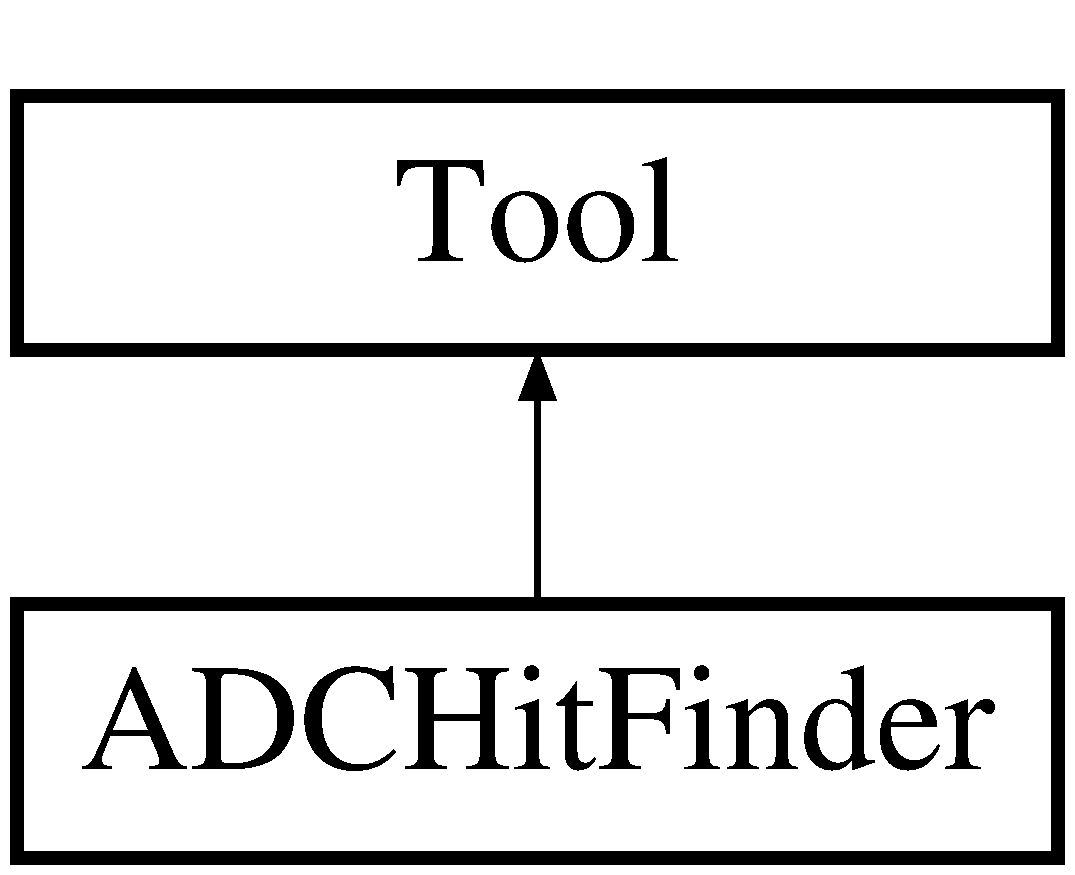
\includegraphics[height=2.000000cm]{classADCHitFinder}
\end{center}
\end{figure}
\subsection*{Public Member Functions}
\begin{DoxyCompactItemize}
\item 
\hypertarget{classADCHitFinder_a944ec97d4451bd6da825a51ddd2481a4}{bool {\bfseries Initialise} (const std\-::string configfile, \hyperlink{classDataModel}{Data\-Model} \&data) override}\label{classADCHitFinder_a944ec97d4451bd6da825a51ddd2481a4}

\item 
\hypertarget{classADCHitFinder_a17e0a0b2622a32902025ec1e2a498a42}{bool {\bfseries Execute} () override}\label{classADCHitFinder_a17e0a0b2622a32902025ec1e2a498a42}

\item 
\hypertarget{classADCHitFinder_a7bc2963aac26cf6dbb5e2be2ed034f60}{bool {\bfseries Finalise} () override}\label{classADCHitFinder_a7bc2963aac26cf6dbb5e2be2ed034f60}

\end{DoxyCompactItemize}
\subsection*{Protected Member Functions}
\begin{DoxyCompactItemize}
\item 
\hypertarget{classADCHitFinder_a1543f5cfc28798facf7dc1bd67697171}{std\-::vector$<$ \hyperlink{classADCPulse}{A\-D\-C\-Pulse} $>$ {\bfseries find\-\_\-pulses} (const \hyperlink{classWaveform}{Waveform}$<$ unsigned short $>$ \&raw\-\_\-minibuffer\-\_\-data, const \hyperlink{classCalibratedADCWaveform}{Calibrated\-A\-D\-C\-Waveform}$<$ double $>$ \&calibrated\-\_\-minibuffer\-\_\-data, unsigned short adc\-\_\-threshold, const unsigned long \&channel\-\_\-key) const }\label{classADCHitFinder_a1543f5cfc28798facf7dc1bd67697171}

\end{DoxyCompactItemize}


The documentation for this class was generated from the following files\-:\begin{DoxyCompactItemize}
\item 
User\-Tools/\-A\-D\-C\-Hit\-Finder/A\-D\-C\-Hit\-Finder.\-h\item 
User\-Tools/\-A\-D\-C\-Hit\-Finder/A\-D\-C\-Hit\-Finder.\-cpp\end{DoxyCompactItemize}

\hypertarget{classADCPulse}{
\section{ADCPulse Class Reference}
\label{classADCPulse}\index{ADCPulse@{ADCPulse}}
}
Inheritance diagram for ADCPulse::\begin{figure}[H]
\begin{center}
\leavevmode
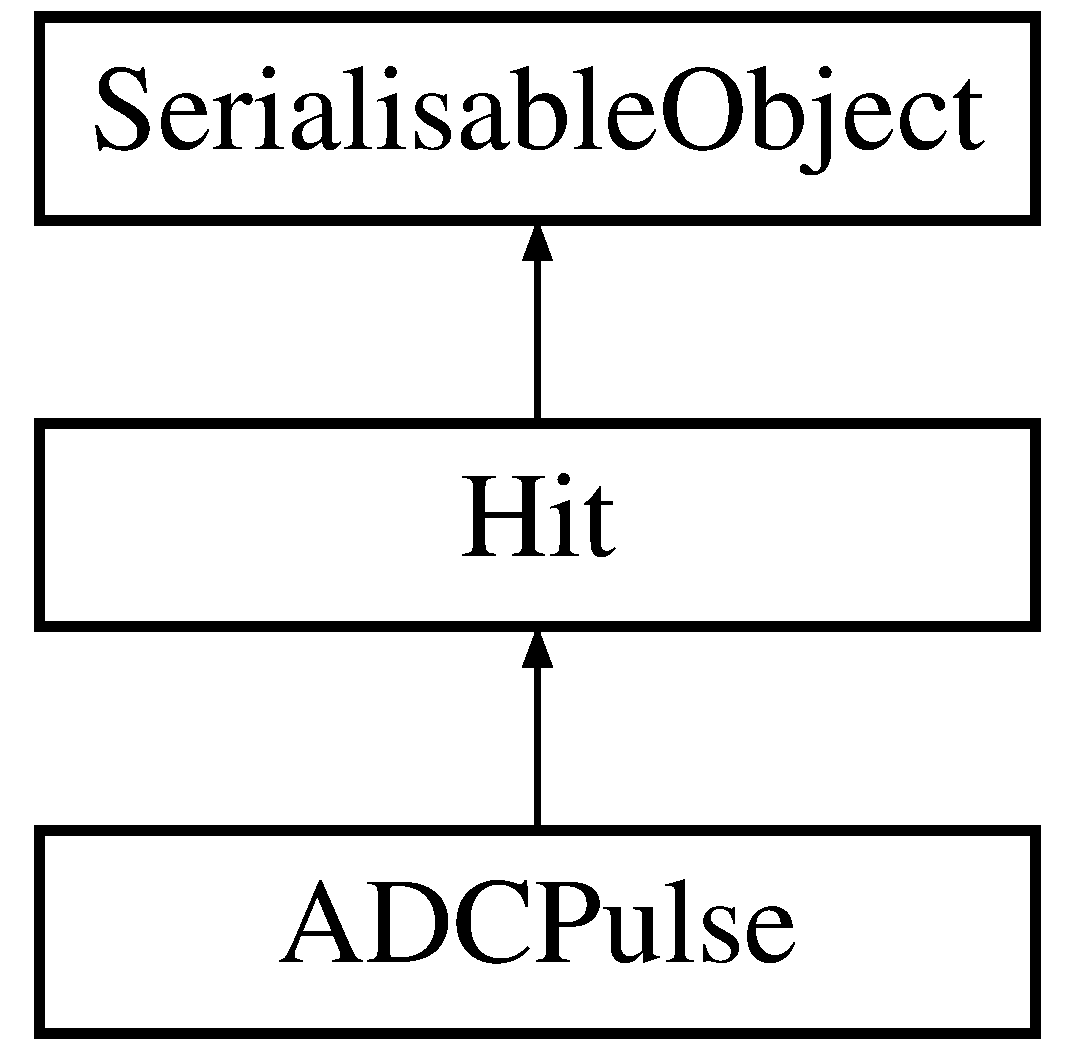
\includegraphics[height=3cm]{classADCPulse}
\end{center}
\end{figure}
\subsection*{Public Member Functions}
\begin{DoxyCompactItemize}
\item 
\hypertarget{classADCPulse_a98b82ea9459a5fca7947a855fb8c7405}{
{\bfseries ADCPulse} (int TubeId, double start\_\-time, double peak\_\-time, double baseline, double sigma\_\-baseline, unsigned long raw\_\-area, unsigned short raw\_\-amplitude, double calibrated\_\-amplitude, double charge)}
\label{classADCPulse_a98b82ea9459a5fca7947a855fb8c7405}

\item 
\hypertarget{classADCPulse_aba2eb2e6400677d592ef1685ba2ae5a9}{
double {\bfseries start\_\-time} () const }
\label{classADCPulse_aba2eb2e6400677d592ef1685ba2ae5a9}

\item 
\hypertarget{classADCPulse_ac55a1faf2cf205fbdc859daece64a021}{
double {\bfseries peak\_\-time} () const }
\label{classADCPulse_ac55a1faf2cf205fbdc859daece64a021}

\item 
\hypertarget{classADCPulse_a4900e0a75c4981491f8609428888a6bc}{
double {\bfseries baseline} () const }
\label{classADCPulse_a4900e0a75c4981491f8609428888a6bc}

\item 
\hypertarget{classADCPulse_a824ed4ba627f7641ff70adf2fe3b026f}{
double {\bfseries sigma\_\-baseline} () const }
\label{classADCPulse_a824ed4ba627f7641ff70adf2fe3b026f}

\item 
\hypertarget{classADCPulse_a692780da124b59770356393f16299c49}{
unsigned long {\bfseries raw\_\-area} () const }
\label{classADCPulse_a692780da124b59770356393f16299c49}

\item 
\hypertarget{classADCPulse_a7a09c65e5b638c6a2df3e437219f04f8}{
unsigned short {\bfseries raw\_\-amplitude} () const }
\label{classADCPulse_a7a09c65e5b638c6a2df3e437219f04f8}

\item 
\hypertarget{classADCPulse_aad38764b5eabe9d858309bc06cf73424}{
double {\bfseries charge} () const }
\label{classADCPulse_aad38764b5eabe9d858309bc06cf73424}

\item 
\hypertarget{classADCPulse_adf6f2ab6b4c28e425dd7567a70099826}{
double {\bfseries amplitude} () const }
\label{classADCPulse_adf6f2ab6b4c28e425dd7567a70099826}

\item 
\hypertarget{classADCPulse_a454d731a107182274df51d3ccf116e52}{
{\footnotesize template$<$class Archive $>$ }\\void {\bfseries serialize} (Archive \&ar, const unsigned int version)}
\label{classADCPulse_a454d731a107182274df51d3ccf116e52}

\end{DoxyCompactItemize}
\subsection*{Protected Attributes}
\begin{DoxyCompactItemize}
\item 
\hypertarget{classADCPulse_af93ef20fa02d9ea44a7b84d32c8b029f}{
double {\bfseries start\_\-time\_\-}}
\label{classADCPulse_af93ef20fa02d9ea44a7b84d32c8b029f}

\item 
\hypertarget{classADCPulse_a4e87f35bcc0f597f6e3c3e73d0b4312b}{
double {\bfseries peak\_\-time\_\-}}
\label{classADCPulse_a4e87f35bcc0f597f6e3c3e73d0b4312b}

\item 
\hypertarget{classADCPulse_ab355ff3d438597f659f899e14e9ce37a}{
double {\bfseries baseline\_\-}}
\label{classADCPulse_ab355ff3d438597f659f899e14e9ce37a}

\item 
\hypertarget{classADCPulse_a97eddbc21ba72324520405c64288693e}{
double {\bfseries sigma\_\-baseline\_\-}}
\label{classADCPulse_a97eddbc21ba72324520405c64288693e}

\item 
\hypertarget{classADCPulse_ae665395493e477287e366b9d8772996d}{
unsigned long {\bfseries raw\_\-area\_\-}}
\label{classADCPulse_ae665395493e477287e366b9d8772996d}

\item 
\hypertarget{classADCPulse_ad77ade03d815b418fe138fd599f3db57}{
unsigned short {\bfseries raw\_\-amplitude\_\-}}
\label{classADCPulse_ad77ade03d815b418fe138fd599f3db57}

\item 
\hypertarget{classADCPulse_ae68ae047968f1257b4aa0ad9bfd08847}{
double {\bfseries calibrated\_\-amplitude\_\-}}
\label{classADCPulse_ae68ae047968f1257b4aa0ad9bfd08847}

\end{DoxyCompactItemize}
\subsection*{Friends}
\begin{DoxyCompactItemize}
\item 
\hypertarget{classADCPulse_ac98d07dd8f7b70e16ccb9a01abf56b9c}{
class {\bfseries boost::serialization::access}}
\label{classADCPulse_ac98d07dd8f7b70e16ccb9a01abf56b9c}

\end{DoxyCompactItemize}


The documentation for this class was generated from the following files:\begin{DoxyCompactItemize}
\item 
DataModel/ADCPulse.h\item 
DataModel/ADCPulse.cpp\end{DoxyCompactItemize}

\hypertarget{classANNIEGeometry}{
\section{ANNIEGeometry Class Reference}
\label{classANNIEGeometry}\index{ANNIEGeometry@{ANNIEGeometry}}
}
\subsection*{Public Types}
\begin{DoxyCompactItemize}
\item 
enum {\bfseries EGeoType} \{ {\bfseries kUnknown} =  -\/1, 
{\bfseries kCylinder} =  0, 
{\bfseries kMailBox} =  1
 \}
\item 
enum {\bfseries EGeoRegion} \{ \par
{\bfseries kTop} =  0, 
{\bfseries kSide} =  1, 
{\bfseries kBottom} =  2, 
{\bfseries kFront} =  10, 
\par
{\bfseries kBack} =  12, 
{\bfseries kLeft} =  20, 
{\bfseries kRight} =  22
 \}
\item 
\hypertarget{classANNIEGeometry_ab5d29d11590e8129e6690899d0f84584}{
typedef enum ANNIEGeometry::EGeoType {\bfseries GeoType\_\-t}}
\label{classANNIEGeometry_ab5d29d11590e8129e6690899d0f84584}

\item 
\hypertarget{classANNIEGeometry_acf5083108f2f5a2d8ee98fe5aaa6e596}{
typedef enum ANNIEGeometry::EGeoRegion {\bfseries GeoRegion\_\-t}}
\label{classANNIEGeometry_acf5083108f2f5a2d8ee98fe5aaa6e596}

\end{DoxyCompactItemize}
\subsection*{Public Member Functions}
\begin{DoxyCompactItemize}
\item 
\hypertarget{classANNIEGeometry_a143bd07247da431b54d152fa7cb5c7cf}{
void {\bfseries SetGeometry} ()}
\label{classANNIEGeometry_a143bd07247da431b54d152fa7cb5c7cf}

\item 
\hypertarget{classANNIEGeometry_ab765a9957be6e19208c25fa0e6603ab7}{
void {\bfseries WriteToFile} (const char $\ast$filename=\char`\"{}annie.geometry.root\char`\"{})}
\label{classANNIEGeometry_ab765a9957be6e19208c25fa0e6603ab7}

\item 
\hypertarget{classANNIEGeometry_a4a2b51837cbc2b52159fde213624f07b}{
int {\bfseries GetGeoConfig} ()}
\label{classANNIEGeometry_a4a2b51837cbc2b52159fde213624f07b}

\item 
\hypertarget{classANNIEGeometry_a181399c8d8d8e1e7deaf5e26fc19f6a2}{
int {\bfseries GetGeoType} ()}
\label{classANNIEGeometry_a181399c8d8d8e1e7deaf5e26fc19f6a2}

\item 
\hypertarget{classANNIEGeometry_af52285d65bb359e199d5516215e9d4b2}{
bool {\bfseries IsCylinder} ()}
\label{classANNIEGeometry_af52285d65bb359e199d5516215e9d4b2}

\item 
\hypertarget{classANNIEGeometry_af4067a89f27815d2be201734cf88ef66}{
double {\bfseries GetCylRadius} ()}
\label{classANNIEGeometry_af4067a89f27815d2be201734cf88ef66}

\item 
\hypertarget{classANNIEGeometry_aeb5d59529df45997aa9e88d439fefbba}{
double {\bfseries GetCylLength} ()}
\label{classANNIEGeometry_aeb5d59529df45997aa9e88d439fefbba}

\item 
\hypertarget{classANNIEGeometry_a3dce208ec7515a6db41b29a222ef7a4c}{
double {\bfseries GetCylFiducialRadius} ()}
\label{classANNIEGeometry_a3dce208ec7515a6db41b29a222ef7a4c}

\item 
\hypertarget{classANNIEGeometry_adda169892f173736e7873a0994fa37b6}{
double {\bfseries GetCylFiducialLength} ()}
\label{classANNIEGeometry_adda169892f173736e7873a0994fa37b6}

\item 
\hypertarget{classANNIEGeometry_a7675f55a9fc15b8b6e2165d641e79df9}{
double {\bfseries GetArea} ()}
\label{classANNIEGeometry_a7675f55a9fc15b8b6e2165d641e79df9}

\item 
\hypertarget{classANNIEGeometry_af0bc51ada0af21236895d9f94f2f84a7}{
double {\bfseries GetVolume} ()}
\label{classANNIEGeometry_af0bc51ada0af21236895d9f94f2f84a7}

\item 
\hypertarget{classANNIEGeometry_aa499d80e72d8d23ea302dac47c47c3ac}{
double {\bfseries GetFiducialVolume} ()}
\label{classANNIEGeometry_aa499d80e72d8d23ea302dac47c47c3ac}

\item 
\hypertarget{classANNIEGeometry_a35e0bbb160a9d8aaf3a343c65d1b3e5b}{
int {\bfseries GetNumPMTs} ()}
\label{classANNIEGeometry_a35e0bbb160a9d8aaf3a343c65d1b3e5b}

\item 
\hypertarget{classANNIEGeometry_ab271fef7650f1f85053e5c332923f1b2}{
double {\bfseries GetPMTRadius} ()}
\label{classANNIEGeometry_ab271fef7650f1f85053e5c332923f1b2}

\item 
\hypertarget{classANNIEGeometry_a6a3acf1871f9114c0a174aa776d4d568}{
double {\bfseries GetPMTCoverage} ()}
\label{classANNIEGeometry_a6a3acf1871f9114c0a174aa776d4d568}

\item 
\hypertarget{classANNIEGeometry_a55663b9489c6c3f8be1d8c8d50ea8ecd}{
double {\bfseries GetPMTSeparation} ()}
\label{classANNIEGeometry_a55663b9489c6c3f8be1d8c8d50ea8ecd}

\item 
\hypertarget{classANNIEGeometry_a7b2de9e107a495f3910d24da60987f67}{
int {\bfseries GetRegion} (int tube)}
\label{classANNIEGeometry_a7b2de9e107a495f3910d24da60987f67}

\item 
\hypertarget{classANNIEGeometry_a401b4205253afe89d87c9e86617fae0f}{
double {\bfseries GetX} (int tube)}
\label{classANNIEGeometry_a401b4205253afe89d87c9e86617fae0f}

\item 
\hypertarget{classANNIEGeometry_afdb90742ba6140a78d022658df6e69fc}{
double {\bfseries GetY} (int tube)}
\label{classANNIEGeometry_afdb90742ba6140a78d022658df6e69fc}

\item 
\hypertarget{classANNIEGeometry_ae4563d14f0b5207fff374b03df026410}{
double {\bfseries GetZ} (int tube)}
\label{classANNIEGeometry_ae4563d14f0b5207fff374b03df026410}

\item 
\hypertarget{classANNIEGeometry_ab645d95b1115f411d24baa5dc868b6fb}{
double {\bfseries GetNormX} (int tube)}
\label{classANNIEGeometry_ab645d95b1115f411d24baa5dc868b6fb}

\item 
\hypertarget{classANNIEGeometry_ab674db08c6e04f3f85d82f9135dbe33d}{
double {\bfseries GetNormY} (int tube)}
\label{classANNIEGeometry_ab674db08c6e04f3f85d82f9135dbe33d}

\item 
\hypertarget{classANNIEGeometry_a8dd59a80f126b58e88ab7d3008cb7001}{
double {\bfseries GetNormZ} (int tube)}
\label{classANNIEGeometry_a8dd59a80f126b58e88ab7d3008cb7001}

\item 
\hypertarget{classANNIEGeometry_a8f607acd58c33b95be136fccd285588d}{
bool {\bfseries InsideDetector} (double x, double y, double z)}
\label{classANNIEGeometry_a8f607acd58c33b95be136fccd285588d}

\item 
\hypertarget{classANNIEGeometry_aad46926236afbfb92498aa1642f21180}{
bool {\bfseries InsideFiducialVolume} (double x, double y, double z)}
\label{classANNIEGeometry_aad46926236afbfb92498aa1642f21180}

\item 
\hypertarget{classANNIEGeometry_a971e6acb3ee5883a3aed577831b053cf}{
bool {\bfseries InsideDetector} (double vx, double vy, double vz, double ex, double ey, double ez)}
\label{classANNIEGeometry_a971e6acb3ee5883a3aed577831b053cf}

\item 
\hypertarget{classANNIEGeometry_a9650b8008ba94cc4b53c59f67406db20}{
double {\bfseries DistanceToEdge} (double x, double y, double z)}
\label{classANNIEGeometry_a9650b8008ba94cc4b53c59f67406db20}

\item 
\hypertarget{classANNIEGeometry_a3febbe7fd335e9618a02522d8d55a944}{
void {\bfseries ProjectToNearEdge} (double x0, double y0, double z0, double px, double py, double pz, double \&x, double \&y, double \&z, int \&region)}
\label{classANNIEGeometry_a3febbe7fd335e9618a02522d8d55a944}

\item 
\hypertarget{classANNIEGeometry_ac3c306909b0de82f5ddcc58de6345b16}{
void {\bfseries ProjectToFarEdge} (double x0, double y0, double z0, double px, double py, double pz, double \&x, double \&y, double \&z, int \&region)}
\label{classANNIEGeometry_ac3c306909b0de82f5ddcc58de6345b16}

\item 
\hypertarget{classANNIEGeometry_a88ff7bd1fcd9ed044c177ebbc875e4af}{
double {\bfseries ForwardProjectionToEdge} (double x, double y, double z, double px, double py, double pz)}
\label{classANNIEGeometry_a88ff7bd1fcd9ed044c177ebbc875e4af}

\item 
\hypertarget{classANNIEGeometry_adcc43a523767429765600b7c103dd5e9}{
double {\bfseries BackwardProjectionToEdge} (double x, double y, double z, double px, double py, double pz)}
\label{classANNIEGeometry_adcc43a523767429765600b7c103dd5e9}

\item 
\hypertarget{classANNIEGeometry_a8b4c2a1c960041a8c36c29c40bde9cb1}{
void {\bfseries ProjectToEdge} (bool useFarEdge, double x0, double y0, double z0, double px, double py, double pz, double \&x, double \&y, double \&z, int \&region)}
\label{classANNIEGeometry_a8b4c2a1c960041a8c36c29c40bde9cb1}

\item 
\hypertarget{classANNIEGeometry_a8b839b45c5eace4880b79d451b6e6f29}{
void {\bfseries XYZtoUV} (int region, double x, double y, double z, double \&u, double \&v)}
\label{classANNIEGeometry_a8b839b45c5eace4880b79d451b6e6f29}

\end{DoxyCompactItemize}
\subsection*{Static Public Member Functions}
\begin{DoxyCompactItemize}
\item 
\hypertarget{classANNIEGeometry_ac5019e6c5628d0381760a43169b1f69c}{
static \hyperlink{classANNIEGeometry}{ANNIEGeometry} $\ast$ {\bfseries Instance} ()}
\label{classANNIEGeometry_ac5019e6c5628d0381760a43169b1f69c}

\item 
\hypertarget{classANNIEGeometry_ad5cc6f1a59adcc81ed32baf70fffe80a}{
static void {\bfseries BuildGeometry} ()}
\label{classANNIEGeometry_ad5cc6f1a59adcc81ed32baf70fffe80a}

\item 
\hypertarget{classANNIEGeometry_a263767eee59a5cf354f3f78ff11efe15}{
static void {\bfseries PrintGeometry} ()}
\label{classANNIEGeometry_a263767eee59a5cf354f3f78ff11efe15}

\item 
\hypertarget{classANNIEGeometry_ae6ac4bbd93009837fb6dd876eec7a558}{
static void {\bfseries WriteGeometry} (const char $\ast$filename=\char`\"{}annie.geometry.root\char`\"{})}
\label{classANNIEGeometry_ae6ac4bbd93009837fb6dd876eec7a558}

\item 
\hypertarget{classANNIEGeometry_a1bb496b1b3f0f3ef86a76dc59571beb7}{
static bool {\bfseries TouchGeometry} ()}
\label{classANNIEGeometry_a1bb496b1b3f0f3ef86a76dc59571beb7}

\item 
\hypertarget{classANNIEGeometry_a8d2c6faa5bdc504fb70967551ad59068}{
static void {\bfseries Reset} ()}
\label{classANNIEGeometry_a8d2c6faa5bdc504fb70967551ad59068}

\item 
\hypertarget{classANNIEGeometry_a6de654c497e0f352fc293cfc87246a0f}{
static void {\bfseries FindCircle} (double x0, double y0, double z0, double x1, double y1, double z1, double x2, double y2, double z2, double \&rx, double \&ry, double \&rz, double \&nx, double \&ny, double \&nz, double \&r)}
\label{classANNIEGeometry_a6de654c497e0f352fc293cfc87246a0f}

\item 
\hypertarget{classANNIEGeometry_ab8f9b0fa3e34b1524146e536cb0d61b8}{
static void {\bfseries FindCircle} (double xp, double yp, double zp, double x0, double y0, double z0, double angle\_\-degrees, double omega\_\-degrees, double \&rx, double \&ry, double \&rz, double \&nx, double \&ny, double \&nz, double \&r)}
\label{classANNIEGeometry_ab8f9b0fa3e34b1524146e536cb0d61b8}

\item 
\hypertarget{classANNIEGeometry_a9b64b97c795a3ff52ff8473b844949ab}{
static void {\bfseries FindCircleOld} (double xp, double yp, double zp, double x0, double y0, double z0, double angle\_\-degrees, double omega\_\-degrees, double \&rx, double \&ry, double \&rz, double \&nx, double \&ny, double \&nz, double \&r)}
\label{classANNIEGeometry_a9b64b97c795a3ff52ff8473b844949ab}

\item 
\hypertarget{classANNIEGeometry_a84d4314f64f749a0a7c9a771805226dc}{
static void {\bfseries FindVertex} (double x0, double y0, double z0, double t0, double x1, double y1, double z1, double t1, double x2, double y2, double z2, double t2, double x3, double y3, double z3, double t3, double \&vxm, double \&vym, double \&vzm, double \&vtm, double \&vxp, double \&vyp, double \&vzp, double \&vtp)}
\label{classANNIEGeometry_a84d4314f64f749a0a7c9a771805226dc}

\item 
\hypertarget{classANNIEGeometry_a3ad5ab10afc05105f6be10e87fb69227}{
static void {\bfseries DistanceToIntersectLine} (double x0, double y0, double z0, double vx, double vy, double vz, double ex, double ey, double ez, double \&x, double \&y, double \&z, double \&L)}
\label{classANNIEGeometry_a3ad5ab10afc05105f6be10e87fb69227}

\item 
\hypertarget{classANNIEGeometry_a7564706390f93705700a15d4cf4f43a6}{
static double {\bfseries DistanceToIntersectLine} (double x0, double y0, double z0, double sx, double sy, double sz, double ex, double ey, double ez, double \&x, double \&y, double \&z)}
\label{classANNIEGeometry_a7564706390f93705700a15d4cf4f43a6}

\item 
\hypertarget{classANNIEGeometry_ac39690635de68c00b8c806fcca9ff597}{
static double {\bfseries DistanceToIntersectLine} (double $\ast$pos, double $\ast$start, double $\ast$end, double $\ast$intersection)}
\label{classANNIEGeometry_ac39690635de68c00b8c806fcca9ff597}

\end{DoxyCompactItemize}


The documentation for this class was generated from the following files:\begin{DoxyCompactItemize}
\item 
DataModel/ANNIEGeometry.h\item 
DataModel/ANNIEGeometry.cpp\end{DoxyCompactItemize}

\hypertarget{classANNIERecoObjectTable}{
\section{ANNIERecoObjectTable Class Reference}
\label{classANNIERecoObjectTable}\index{ANNIERecoObjectTable@{ANNIERecoObjectTable}}
}
\subsection*{Public Member Functions}
\begin{DoxyCompactItemize}
\item 
\hypertarget{classANNIERecoObjectTable_ae2e86010f9f57ce6044d084ec40f475b}{
void {\bfseries NewDigit} ()}
\label{classANNIERecoObjectTable_ae2e86010f9f57ce6044d084ec40f475b}

\item 
\hypertarget{classANNIERecoObjectTable_a75f289f8c9eef9098813dbdcc8ddd518}{
void {\bfseries DeleteDigit} ()}
\label{classANNIERecoObjectTable_a75f289f8c9eef9098813dbdcc8ddd518}

\item 
\hypertarget{classANNIERecoObjectTable_a6a91ff418f86119ef35de20c5c9a9e8a}{
Int\_\-t {\bfseries NumberOfDigits} ()}
\label{classANNIERecoObjectTable_a6a91ff418f86119ef35de20c5c9a9e8a}

\item 
\hypertarget{classANNIERecoObjectTable_a4bbb7e3eb5ca8a46486a1087ef2b4ff1}{
void {\bfseries NewCluster} ()}
\label{classANNIERecoObjectTable_a4bbb7e3eb5ca8a46486a1087ef2b4ff1}

\item 
\hypertarget{classANNIERecoObjectTable_a77fe22b611dbc374779bf258eae901a2}{
void {\bfseries DeleteCluster} ()}
\label{classANNIERecoObjectTable_a77fe22b611dbc374779bf258eae901a2}

\item 
\hypertarget{classANNIERecoObjectTable_a87c83bd73d95b7bc2fca9855e8604496}{
Int\_\-t {\bfseries NumberOfClusters} ()}
\label{classANNIERecoObjectTable_a87c83bd73d95b7bc2fca9855e8604496}

\item 
\hypertarget{classANNIERecoObjectTable_ae5d19c03be8a404512ddad75e76be951}{
void {\bfseries NewClusterDigit} ()}
\label{classANNIERecoObjectTable_ae5d19c03be8a404512ddad75e76be951}

\item 
\hypertarget{classANNIERecoObjectTable_ae9e239382fa31db834474b4307959f1b}{
void {\bfseries DeleteClusterDigit} ()}
\label{classANNIERecoObjectTable_ae9e239382fa31db834474b4307959f1b}

\item 
\hypertarget{classANNIERecoObjectTable_a6b1f8a751bd988ea99bb1dcd04e355f1}{
Int\_\-t {\bfseries NumberOfClusterDigits} ()}
\label{classANNIERecoObjectTable_a6b1f8a751bd988ea99bb1dcd04e355f1}

\item 
\hypertarget{classANNIERecoObjectTable_a27ba37a8270a06fd8a60334e94c5ccc7}{
void {\bfseries NewVertex} ()}
\label{classANNIERecoObjectTable_a27ba37a8270a06fd8a60334e94c5ccc7}

\item 
\hypertarget{classANNIERecoObjectTable_a51a949a392b138359f6c3e3a91a17815}{
void {\bfseries DeleteVertex} ()}
\label{classANNIERecoObjectTable_a51a949a392b138359f6c3e3a91a17815}

\item 
\hypertarget{classANNIERecoObjectTable_ad96ca7367ce386c39b33fe7028481fed}{
Int\_\-t {\bfseries NumberOfVertices} ()}
\label{classANNIERecoObjectTable_ad96ca7367ce386c39b33fe7028481fed}

\item 
\hypertarget{classANNIERecoObjectTable_a44fea21839a6a27ea162659799d64b9e}{
void {\bfseries NewRing} ()}
\label{classANNIERecoObjectTable_a44fea21839a6a27ea162659799d64b9e}

\item 
\hypertarget{classANNIERecoObjectTable_a91992ce4b239b292ea3e8300b6f3d051}{
void {\bfseries DeleteRing} ()}
\label{classANNIERecoObjectTable_a91992ce4b239b292ea3e8300b6f3d051}

\item 
\hypertarget{classANNIERecoObjectTable_a6f4586ab138e3de6e2d0445f9a42158e}{
Int\_\-t {\bfseries NumberOfRings} ()}
\label{classANNIERecoObjectTable_a6f4586ab138e3de6e2d0445f9a42158e}

\item 
\hypertarget{classANNIERecoObjectTable_a40d63437190711714ef1a0e2323e552b}{
void {\bfseries NewEvent} ()}
\label{classANNIERecoObjectTable_a40d63437190711714ef1a0e2323e552b}

\item 
\hypertarget{classANNIERecoObjectTable_ad9e81e1ef88bb6c19359465cf1897489}{
void {\bfseries DeleteEvent} ()}
\label{classANNIERecoObjectTable_ad9e81e1ef88bb6c19359465cf1897489}

\item 
\hypertarget{classANNIERecoObjectTable_a2802d7f20a163c710703ede7b66ba02f}{
Int\_\-t {\bfseries NumberOfEvents} ()}
\label{classANNIERecoObjectTable_a2802d7f20a163c710703ede7b66ba02f}

\item 
\hypertarget{classANNIERecoObjectTable_ae0f39f0d4b6392330fe449f22b3a5481}{
void {\bfseries Reset} ()}
\label{classANNIERecoObjectTable_ae0f39f0d4b6392330fe449f22b3a5481}

\item 
\hypertarget{classANNIERecoObjectTable_a620e131ba8cf125b7f08f25d19ee14c1}{
void {\bfseries Print} ()}
\label{classANNIERecoObjectTable_a620e131ba8cf125b7f08f25d19ee14c1}

\end{DoxyCompactItemize}
\subsection*{Static Public Member Functions}
\begin{DoxyCompactItemize}
\item 
\hypertarget{classANNIERecoObjectTable_a2d52c0a9b2ed24f59c97ae6cfff3b1f6}{
static \hyperlink{classANNIERecoObjectTable}{ANNIERecoObjectTable} $\ast$ {\bfseries Instance} ()}
\label{classANNIERecoObjectTable_a2d52c0a9b2ed24f59c97ae6cfff3b1f6}

\end{DoxyCompactItemize}


The documentation for this class was generated from the following files:\begin{DoxyCompactItemize}
\item 
DataModel/ANNIERecoObjectTable.h\item 
DataModel/ANNIERecoObjectTable.cpp\end{DoxyCompactItemize}

\hypertarget{classBeamChecker}{\section{Beam\-Checker Class Reference}
\label{classBeamChecker}\index{Beam\-Checker@{Beam\-Checker}}
}
Inheritance diagram for Beam\-Checker\-:\begin{figure}[H]
\begin{center}
\leavevmode
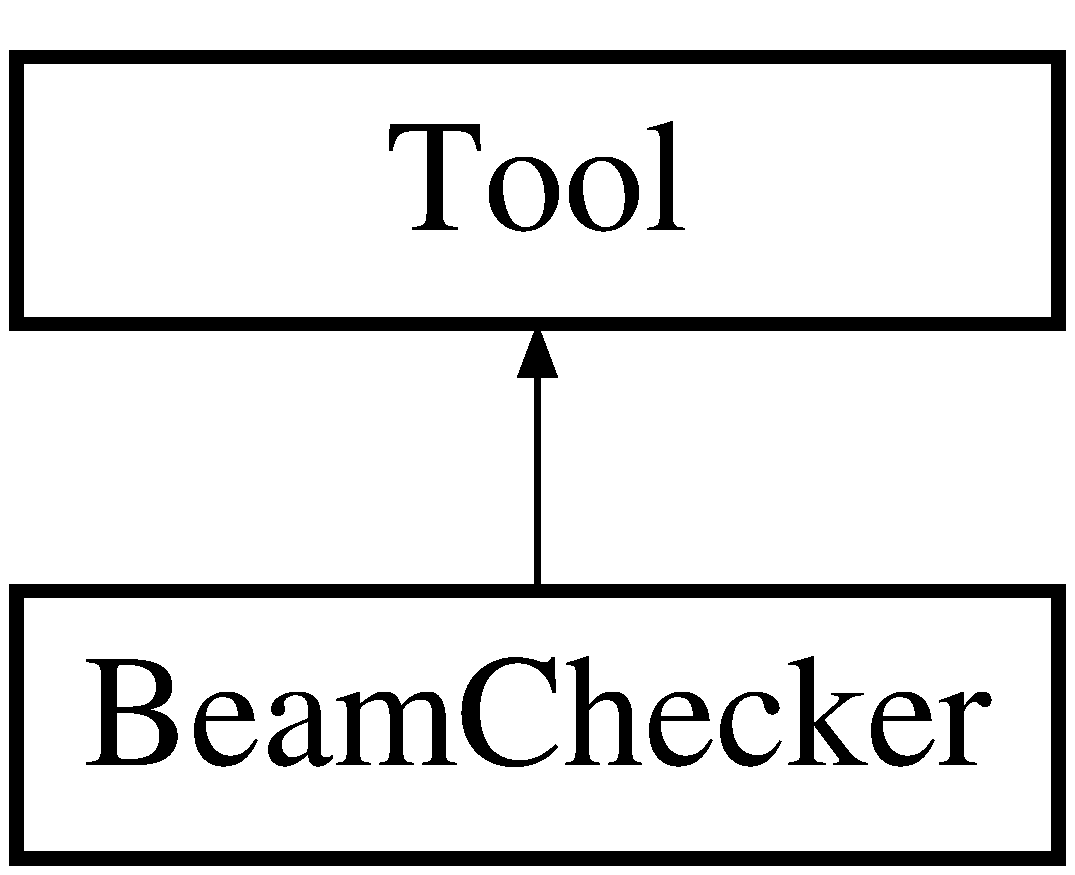
\includegraphics[height=2.000000cm]{classBeamChecker}
\end{center}
\end{figure}
\subsection*{Public Member Functions}
\begin{DoxyCompactItemize}
\item 
\hypertarget{classBeamChecker_a8025fea06b24c363f17764b3cc049ebd}{bool {\bfseries Initialise} (std\-::string configfile, \hyperlink{classDataModel}{Data\-Model} \&data)}\label{classBeamChecker_a8025fea06b24c363f17764b3cc049ebd}

\item 
\hypertarget{classBeamChecker_a9fd96575f736c2a0a90e9b18fca3bdf7}{bool {\bfseries Execute} ()}\label{classBeamChecker_a9fd96575f736c2a0a90e9b18fca3bdf7}

\item 
\hypertarget{classBeamChecker_a1f9078a610f387f97dc6d17a6b98f493}{bool {\bfseries Finalise} ()}\label{classBeamChecker_a1f9078a610f387f97dc6d17a6b98f493}

\end{DoxyCompactItemize}
\subsection*{Protected Member Functions}
\begin{DoxyCompactItemize}
\item 
\hypertarget{classBeamChecker_a85643380e26692a3fad55cc4e7d4ea1b}{bool \hyperlink{classBeamChecker_a85643380e26692a3fad55cc4e7d4ea1b}{initialise\-\_\-beam\-\_\-db} ()}\label{classBeamChecker_a85643380e26692a3fad55cc4e7d4ea1b}

\begin{DoxyCompactList}\small\item\em Helper function that opens the beam database data file and loads the Beam\-D\-B Boost\-Store. \end{DoxyCompactList}\item 
\hypertarget{classBeamChecker_a40e731049d58aa141a15f3431b00a764}{\hyperlink{classBeamStatus}{Beam\-Status} {\bfseries get\-\_\-beam\-\_\-status} (uint64\-\_\-t ns\-\_\-since\-\_\-epoch, Minibuffer\-Label mb\-\_\-label)}\label{classBeamChecker_a40e731049d58aa141a15f3431b00a764}

\end{DoxyCompactItemize}
\subsection*{Protected Attributes}
\begin{DoxyCompactItemize}
\item 
\hypertarget{classBeamChecker_a2b910738f1f07819ce8cf564bff685d0}{Boost\-Store \hyperlink{classBeamChecker_a2b910738f1f07819ce8cf564bff685d0}{beam\-\_\-db\-\_\-store\-\_\-}}\label{classBeamChecker_a2b910738f1f07819ce8cf564bff685d0}

\begin{DoxyCompactList}\small\item\em Transient Boost\-Store used to read previously-\/saved information from the beam database. \end{DoxyCompactList}\item 
std\-::map$<$ int, std\-::pair\\*
$<$ uint64\-\_\-t, uint64\-\_\-t $>$ $>$ \hyperlink{classBeamChecker_aab9b16fbdd8cdea6aa1a77fc2f0ea842}{beam\-\_\-db\-\_\-index\-\_\-}
\begin{DoxyCompactList}\small\item\em Map that enables quick searches of the beam database Boost\-Store. \end{DoxyCompactList}\item 
int \hyperlink{classBeamChecker_aceafb01556c2541a737d4feaab2f757e}{verbosity\-\_\-}
\begin{DoxyCompactList}\small\item\em The verbosity to use when printing logging messages. \end{DoxyCompactList}\item 
\hypertarget{classBeamChecker_acd0db6480aaf42ee431b182a68496c32}{uint64\-\_\-t \hyperlink{classBeamChecker_acd0db6480aaf42ee431b182a68496c32}{start\-\_\-ms\-\_\-since\-\_\-epoch\-\_\-}}\label{classBeamChecker_acd0db6480aaf42ee431b182a68496c32}

\begin{DoxyCompactList}\small\item\em The timestamp (ms since the Unix epoch) of the earliest P\-O\-T information available in the current beam database file. \end{DoxyCompactList}\item 
\hypertarget{classBeamChecker_abb2801b7c15da8c7ae56f96786d6cb54}{uint64\-\_\-t \hyperlink{classBeamChecker_abb2801b7c15da8c7ae56f96786d6cb54}{end\-\_\-ms\-\_\-since\-\_\-epoch\-\_\-}}\label{classBeamChecker_abb2801b7c15da8c7ae56f96786d6cb54}

\begin{DoxyCompactList}\small\item\em The timestamp (ms since the Unix epoch) of the latest P\-O\-T information available in the current beam database file. \end{DoxyCompactList}\end{DoxyCompactItemize}


\subsection{Member Data Documentation}
\hypertarget{classBeamChecker_aab9b16fbdd8cdea6aa1a77fc2f0ea842}{\index{Beam\-Checker@{Beam\-Checker}!beam\-\_\-db\-\_\-index\-\_\-@{beam\-\_\-db\-\_\-index\-\_\-}}
\index{beam\-\_\-db\-\_\-index\-\_\-@{beam\-\_\-db\-\_\-index\-\_\-}!BeamChecker@{Beam\-Checker}}
\subsubsection[{beam\-\_\-db\-\_\-index\-\_\-}]{\setlength{\rightskip}{0pt plus 5cm}std\-::map$<$int, std\-::pair$<$uint64\-\_\-t, uint64\-\_\-t$>$ $>$ Beam\-Checker\-::beam\-\_\-db\-\_\-index\-\_\-\hspace{0.3cm}{\ttfamily [protected]}}}\label{classBeamChecker_aab9b16fbdd8cdea6aa1a77fc2f0ea842}


Map that enables quick searches of the beam database Boost\-Store. 

Keys are entry numbers in the Beam\-Data T\-Tree, values are (start time, end time) pairs giving the range of times (in ms since the Unix epoch) recorded for the E\-:T\-O\-R875 device (used to determine P\-O\-T values) in each entry \hypertarget{classBeamChecker_aceafb01556c2541a737d4feaab2f757e}{\index{Beam\-Checker@{Beam\-Checker}!verbosity\-\_\-@{verbosity\-\_\-}}
\index{verbosity\-\_\-@{verbosity\-\_\-}!BeamChecker@{Beam\-Checker}}
\subsubsection[{verbosity\-\_\-}]{\setlength{\rightskip}{0pt plus 5cm}int Beam\-Checker\-::verbosity\-\_\-\hspace{0.3cm}{\ttfamily [protected]}}}\label{classBeamChecker_aceafb01556c2541a737d4feaab2f757e}


The verbosity to use when printing logging messages. 

A larger value corresponds to more verbose output 

The documentation for this class was generated from the following files\-:\begin{DoxyCompactItemize}
\item 
User\-Tools/\-Beam\-Checker/Beam\-Checker.\-h\item 
User\-Tools/\-Beam\-Checker/Beam\-Checker.\-cpp\end{DoxyCompactItemize}

\hypertarget{structBeamDataPoint}{\section{Beam\-Data\-Point Struct Reference}
\label{structBeamDataPoint}\index{Beam\-Data\-Point@{Beam\-Data\-Point}}
}


Container to hold values from Intensity Frontier beam database queries, together with their associated units.  




{\ttfamily \#include $<$Beam\-Data\-Point.\-h$>$}

Inheritance diagram for Beam\-Data\-Point\-:\begin{figure}[H]
\begin{center}
\leavevmode
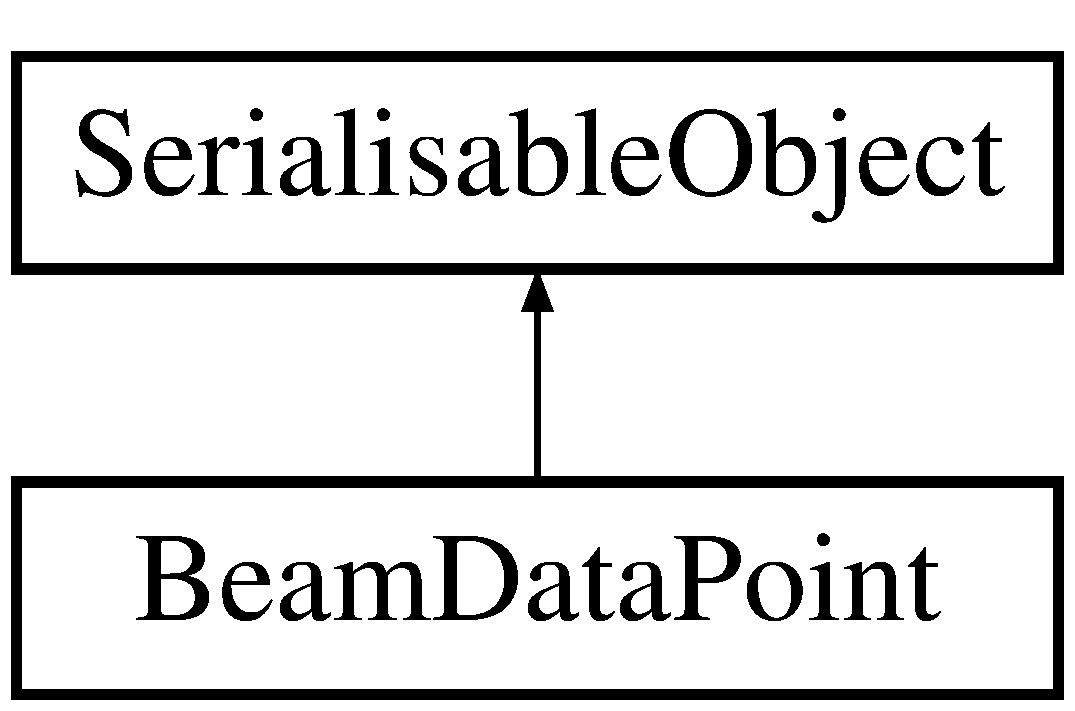
\includegraphics[height=2.000000cm]{structBeamDataPoint}
\end{center}
\end{figure}
\subsection*{Public Member Functions}
\begin{DoxyCompactItemize}
\item 
\hypertarget{structBeamDataPoint_ad98646938f8e5337563523d7d0a198b4}{{\bfseries Beam\-Data\-Point} (double Value, const std\-::string \&Unit)}\label{structBeamDataPoint_ad98646938f8e5337563523d7d0a198b4}

\item 
\hypertarget{structBeamDataPoint_a6369107cfd88d05e8b434da0e234d546}{{\footnotesize template$<$class Archive $>$ }\\void {\bfseries serialize} (Archive \&ar, const unsigned int version)}\label{structBeamDataPoint_a6369107cfd88d05e8b434da0e234d546}

\item 
\hypertarget{structBeamDataPoint_aaa7b4c28dfad7d79f92c6d60001d36ac}{virtual bool {\bfseries Print} () override}\label{structBeamDataPoint_aaa7b4c28dfad7d79f92c6d60001d36ac}

\end{DoxyCompactItemize}
\subsection*{Public Attributes}
\begin{DoxyCompactItemize}
\item 
\hypertarget{structBeamDataPoint_ab877fc81dd293f30ec6475f9649cddd0}{double {\bfseries value}}\label{structBeamDataPoint_ab877fc81dd293f30ec6475f9649cddd0}

\item 
\hypertarget{structBeamDataPoint_a0a0e275d6a6bc2631c4103eb7e2b44e4}{std\-::string {\bfseries unit}}\label{structBeamDataPoint_a0a0e275d6a6bc2631c4103eb7e2b44e4}

\end{DoxyCompactItemize}
\subsection*{Friends}
\begin{DoxyCompactItemize}
\item 
\hypertarget{structBeamDataPoint_ac98d07dd8f7b70e16ccb9a01abf56b9c}{class {\bfseries boost\-::serialization\-::access}}\label{structBeamDataPoint_ac98d07dd8f7b70e16ccb9a01abf56b9c}

\end{DoxyCompactItemize}


\subsection{Detailed Description}
Container to hold values from Intensity Frontier beam database queries, together with their associated units. 

The documentation for this struct was generated from the following file\-:\begin{DoxyCompactItemize}
\item 
Data\-Model/Beam\-Data\-Point.\-h\end{DoxyCompactItemize}

\hypertarget{classBeamFetcher}{\section{Beam\-Fetcher Class Reference}
\label{classBeamFetcher}\index{Beam\-Fetcher@{Beam\-Fetcher}}
}
Inheritance diagram for Beam\-Fetcher\-:\begin{figure}[H]
\begin{center}
\leavevmode
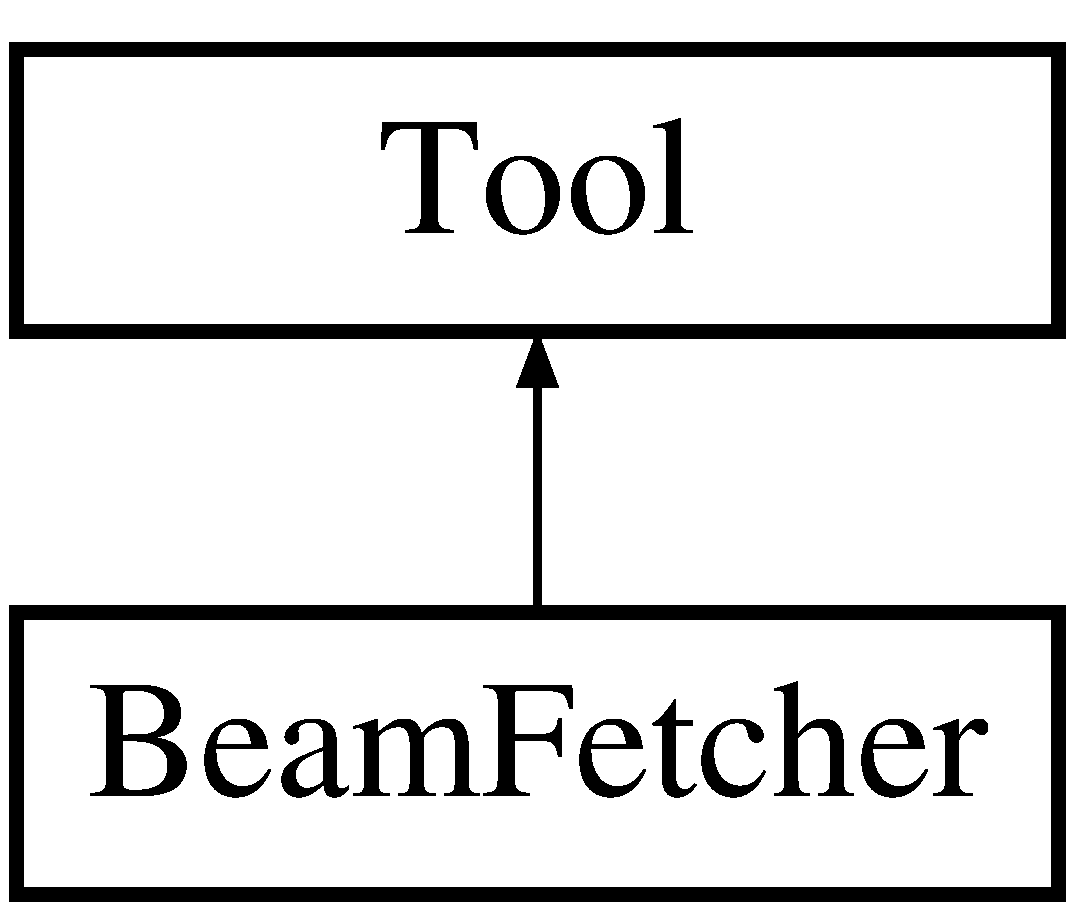
\includegraphics[height=2.000000cm]{classBeamFetcher}
\end{center}
\end{figure}
\subsection*{Public Member Functions}
\begin{DoxyCompactItemize}
\item 
\hypertarget{classBeamFetcher_a575275aab7b03eb11cafd132fcce3015}{bool {\bfseries Initialise} (std\-::string configfile, \hyperlink{classDataModel}{Data\-Model} \&data)}\label{classBeamFetcher_a575275aab7b03eb11cafd132fcce3015}

\item 
\hypertarget{classBeamFetcher_afb3681ee1fbe9ea81c6268af05b90a5f}{bool {\bfseries Execute} ()}\label{classBeamFetcher_afb3681ee1fbe9ea81c6268af05b90a5f}

\item 
\hypertarget{classBeamFetcher_ae69fe473f0e6d24685eb9e234d97d172}{bool {\bfseries Finalise} ()}\label{classBeamFetcher_ae69fe473f0e6d24685eb9e234d97d172}

\end{DoxyCompactItemize}
\subsection*{Protected Member Functions}
\begin{DoxyCompactItemize}
\item 
\hypertarget{classBeamFetcher_a60c8d28364654bc042de262cacc94dcb}{bool \hyperlink{classBeamFetcher_a60c8d28364654bc042de262cacc94dcb}{fetch\-\_\-beam\-\_\-data} (uint64\-\_\-t start\-\_\-ms\-\_\-since\-\_\-epoch, uint64\-\_\-t end\-\_\-ms\-\_\-since\-\_\-epoch, uint64\-\_\-t chunk\-\_\-step\-\_\-ms)}\label{classBeamFetcher_a60c8d28364654bc042de262cacc94dcb}

\begin{DoxyCompactList}\small\item\em Helper function that downloads and processes the beam information. \end{DoxyCompactList}\end{DoxyCompactItemize}
\subsection*{Protected Attributes}
\begin{DoxyCompactItemize}
\item 
int \hyperlink{classBeamFetcher_ab78e5092f1cd5b0544fe6b587282c968}{verbosity\-\_\-}
\begin{DoxyCompactList}\small\item\em The verbosity to use when printing logging messages. \end{DoxyCompactList}\item 
\hypertarget{classBeamFetcher_ac9e8e1c53a2f06c00be83258be22400d}{Boost\-Store \hyperlink{classBeamFetcher_ac9e8e1c53a2f06c00be83258be22400d}{beam\-\_\-db\-\_\-store\-\_\-}}\label{classBeamFetcher_ac9e8e1c53a2f06c00be83258be22400d}

\begin{DoxyCompactList}\small\item\em Transient Boost\-Store used to save downloaded information from the Intensity Frontier beam database to disk. \end{DoxyCompactList}\item 
\hypertarget{classBeamFetcher_a6e37759beec5bc578d7d4de539329bce}{std\-::string \hyperlink{classBeamFetcher_a6e37759beec5bc578d7d4de539329bce}{db\-\_\-filename\-\_\-}}\label{classBeamFetcher_a6e37759beec5bc578d7d4de539329bce}

\begin{DoxyCompactList}\small\item\em Name of the output file in which the beam database information will be saved. \end{DoxyCompactList}\end{DoxyCompactItemize}


\subsection{Member Data Documentation}
\hypertarget{classBeamFetcher_ab78e5092f1cd5b0544fe6b587282c968}{\index{Beam\-Fetcher@{Beam\-Fetcher}!verbosity\-\_\-@{verbosity\-\_\-}}
\index{verbosity\-\_\-@{verbosity\-\_\-}!BeamFetcher@{Beam\-Fetcher}}
\subsubsection[{verbosity\-\_\-}]{\setlength{\rightskip}{0pt plus 5cm}int Beam\-Fetcher\-::verbosity\-\_\-\hspace{0.3cm}{\ttfamily [protected]}}}\label{classBeamFetcher_ab78e5092f1cd5b0544fe6b587282c968}


The verbosity to use when printing logging messages. 

A larger value corresponds to more verbose output 

The documentation for this class was generated from the following files\-:\begin{DoxyCompactItemize}
\item 
User\-Tools/\-Beam\-Fetcher/Beam\-Fetcher.\-h\item 
User\-Tools/\-Beam\-Fetcher/Beam\-Fetcher.\-cpp\end{DoxyCompactItemize}

\hypertarget{classBeamStatus}{
\section{BeamStatus Class Reference}
\label{classBeamStatus}\index{BeamStatus@{BeamStatus}}
}
Inheritance diagram for BeamStatus::\begin{figure}[H]
\begin{center}
\leavevmode
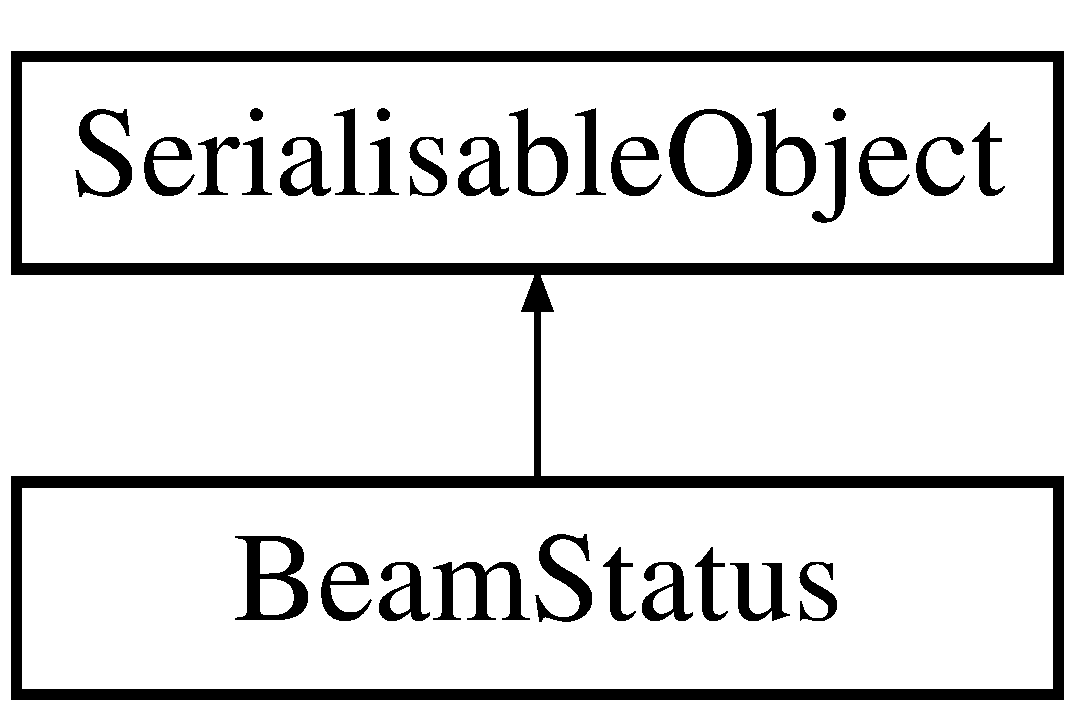
\includegraphics[height=2cm]{classBeamStatus}
\end{center}
\end{figure}
\subsection*{Public Member Functions}
\begin{DoxyCompactItemize}
\item 
\hypertarget{classBeamStatus_a8763cbecad2a03bdc4d4799fd2d68569}{
{\bfseries BeamStatus} (\hyperlink{classTimeClass}{TimeClass} time, double POT, BeamCondition condition=BeamCondition::Missing)}
\label{classBeamStatus_a8763cbecad2a03bdc4d4799fd2d68569}

\item 
\hypertarget{classBeamStatus_ad9786a1628d6180d3abbc74daef3d677}{
void {\bfseries clear} ()}
\label{classBeamStatus_ad9786a1628d6180d3abbc74daef3d677}

\item 
\hypertarget{classBeamStatus_a041fe2a720d2c24391fdaa578754e315}{
\hyperlink{classTimeClass}{TimeClass} {\bfseries time} () const }
\label{classBeamStatus_a041fe2a720d2c24391fdaa578754e315}

\item 
\hypertarget{classBeamStatus_a234b45ea673b396d29b4a40061c633c9}{
double {\bfseries pot} () const }
\label{classBeamStatus_a234b45ea673b396d29b4a40061c633c9}

\item 
\hypertarget{classBeamStatus_a1e0b28ff6f6e0fdc60242e395d836dca}{
BeamCondition {\bfseries condition} () const }
\label{classBeamStatus_a1e0b28ff6f6e0fdc60242e395d836dca}

\item 
\hypertarget{classBeamStatus_a0d1a612eece988337b69b39b73d8170e}{
const std::map$<$ std::string, std::pair$<$ uint64\_\-t, \hyperlink{structBeamDataPoint}{BeamDataPoint} $>$ $>$ \& {\bfseries data} () const }
\label{classBeamStatus_a0d1a612eece988337b69b39b73d8170e}

\item 
\hypertarget{classBeamStatus_a4b0a3f4fcce7aa7e3fa1e62c6f833d57}{
const std::map$<$ std::string, bool $>$ \& {\bfseries cuts} () const }
\label{classBeamStatus_a4b0a3f4fcce7aa7e3fa1e62c6f833d57}

\item 
\hypertarget{classBeamStatus_a106c1657c2cc64e76fac1179ba411485}{
bool {\bfseries is\_\-beam} () const }
\label{classBeamStatus_a106c1657c2cc64e76fac1179ba411485}

\item 
\hypertarget{classBeamStatus_a81a21d4debb9d1497024398bd8834ba3}{
bool {\bfseries is\_\-missing} () const }
\label{classBeamStatus_a81a21d4debb9d1497024398bd8834ba3}

\item 
\hypertarget{classBeamStatus_af51602157cd9beb020fd01cc72dd95cd}{
bool {\bfseries is\_\-bad} () const }
\label{classBeamStatus_af51602157cd9beb020fd01cc72dd95cd}

\item 
\hypertarget{classBeamStatus_aba458d6774b27d401b393de038668849}{
bool {\bfseries ok} () const }
\label{classBeamStatus_aba458d6774b27d401b393de038668849}

\item 
\hypertarget{classBeamStatus_ab6b42b298203d0df45cfb46686d491c2}{
bool {\bfseries passed\_\-cut} (const std::string \&cut\_\-name) const }
\label{classBeamStatus_ab6b42b298203d0df45cfb46686d491c2}

\item 
\hypertarget{classBeamStatus_a34ae2eee9aeb8bfe54d176455e6caaa4}{
bool {\bfseries passed\_\-all\_\-cuts} () const }
\label{classBeamStatus_a34ae2eee9aeb8bfe54d176455e6caaa4}

\item 
\hypertarget{classBeamStatus_aa92b44fce12d6ed0a9a14adcdb95487a}{
void {\bfseries set\_\-time} (\hyperlink{classTimeClass}{TimeClass} time)}
\label{classBeamStatus_aa92b44fce12d6ed0a9a14adcdb95487a}

\item 
\hypertarget{classBeamStatus_a298a8def6b655bf601a73cd0f27ec5b1}{
void {\bfseries set\_\-pot} (double POT)}
\label{classBeamStatus_a298a8def6b655bf601a73cd0f27ec5b1}

\item 
\hypertarget{classBeamStatus_aff21cffb9bcc0562b0940839f80b30f4}{
void {\bfseries set\_\-condition} (BeamCondition bc)}
\label{classBeamStatus_aff21cffb9bcc0562b0940839f80b30f4}

\item 
\hypertarget{classBeamStatus_a088f4dc4e0db476f939314e6c596ee1c}{
void {\bfseries add\_\-measurement} (const std::string \&device\_\-name, uint64\_\-t ms\_\-since\_\-epoch, const \hyperlink{structBeamDataPoint}{BeamDataPoint} \&bdp)}
\label{classBeamStatus_a088f4dc4e0db476f939314e6c596ee1c}

\item 
\hypertarget{classBeamStatus_a5ea13f02f3addd9c9cfc406d461db5db}{
void {\bfseries add\_\-measurement} (const std::string \&device\_\-name, uint64\_\-t ms\_\-since\_\-epoch, double value, const std::string \&unit)}
\label{classBeamStatus_a5ea13f02f3addd9c9cfc406d461db5db}

\item 
\hypertarget{classBeamStatus_add23dfa0ed263857cd9f734815051b9a}{
void {\bfseries add\_\-cut} (const std::string \&cut\_\-name, bool passed)}
\label{classBeamStatus_add23dfa0ed263857cd9f734815051b9a}

\item 
\hypertarget{classBeamStatus_a9c074d793c6a5e55d12265895c736d9e}{
bool {\bfseries Print} ()}
\label{classBeamStatus_a9c074d793c6a5e55d12265895c736d9e}

\end{DoxyCompactItemize}
\subsection*{Protected Member Functions}
\begin{DoxyCompactItemize}
\item 
\hypertarget{classBeamStatus_a20411754c151c9e8afc6fc7e215a3475}{
{\footnotesize template$<$class Archive $>$ }\\void {\bfseries serialize} (Archive \&ar, const unsigned int version)}
\label{classBeamStatus_a20411754c151c9e8afc6fc7e215a3475}

\end{DoxyCompactItemize}
\subsection*{Protected Attributes}
\begin{DoxyCompactItemize}
\item 
\hyperlink{classTimeClass}{TimeClass} \hyperlink{classBeamStatus_a499b220ec0c80ce883d19f8f9520934d}{time\_\-}
\begin{DoxyCompactList}\small\item\em The timestamp from the beam database used to assign a POT value to the current minibuffer (ns since the Unix epoch). \item\end{DoxyCompactList}\item 
\hypertarget{classBeamStatus_ab4d86e7e924a02a73324105931e5bdc5}{
double \hyperlink{classBeamStatus_ab4d86e7e924a02a73324105931e5bdc5}{pot\_\-}}
\label{classBeamStatus_ab4d86e7e924a02a73324105931e5bdc5}

\begin{DoxyCompactList}\small\item\em Protons on target. \item\end{DoxyCompactList}\item 
BeamCondition \hyperlink{classBeamStatus_a8e81a7fca77f64c2ce0e41bd0e14c3ea}{condition\_\-}
\begin{DoxyCompactList}\small\item\em Enum class describing whether the data can be trusted. \item\end{DoxyCompactList}\item 
\hypertarget{classBeamStatus_a784e81454e78fc90f3c8206d68cae144}{
std::map$<$ std::string, std::pair$<$ uint64\_\-t, \hyperlink{structBeamDataPoint}{BeamDataPoint} $>$ $>$ {\bfseries data\_\-}}
\label{classBeamStatus_a784e81454e78fc90f3c8206d68cae144}

\item 
\hypertarget{classBeamStatus_aff0365d2d921712d77e96fabfbcebdc3}{
std::map$<$ std::string, bool $>$ {\bfseries cuts\_\-}}
\label{classBeamStatus_aff0365d2d921712d77e96fabfbcebdc3}

\end{DoxyCompactItemize}
\subsection*{Friends}
\begin{DoxyCompactItemize}
\item 
\hypertarget{classBeamStatus_ac98d07dd8f7b70e16ccb9a01abf56b9c}{
class {\bfseries boost::serialization::access}}
\label{classBeamStatus_ac98d07dd8f7b70e16ccb9a01abf56b9c}

\end{DoxyCompactItemize}


\subsection{Member Data Documentation}
\hypertarget{classBeamStatus_a8e81a7fca77f64c2ce0e41bd0e14c3ea}{
\index{BeamStatus@{BeamStatus}!condition\_\-@{condition\_\-}}
\index{condition\_\-@{condition\_\-}!BeamStatus@{BeamStatus}}
\subsubsection[{condition\_\-}]{\setlength{\rightskip}{0pt plus 5cm}BeamCondition {\bf BeamStatus::condition\_\-}\hspace{0.3cm}{\ttfamily  \mbox{[}protected\mbox{]}}}}
\label{classBeamStatus_a8e81a7fca77f64c2ce0e41bd0e14c3ea}


Enum class describing whether the data can be trusted. Minibuffers arising from something other than beam triggers should all be marked as \char`\"{}NonBeamMinibuffer\char`\"{}. Beam minibuffers should be marked as \char`\"{}Ok\char`\"{}, \char`\"{}Missing\char`\"{} (a query to the beam database failed), or \char`\"{}Bad\char`\"{} (beam information was retrieved successfully, but the current beam spill should be ignored in the analysis). Reasons for marking a beam minibuffer as \char`\"{}Bad\char`\"{} include a very low POT value (suggesting that the beam monitor E:TOR875 was off at the time), a low peak horn current, etc. \hypertarget{classBeamStatus_a499b220ec0c80ce883d19f8f9520934d}{
\index{BeamStatus@{BeamStatus}!time\_\-@{time\_\-}}
\index{time\_\-@{time\_\-}!BeamStatus@{BeamStatus}}
\subsubsection[{time\_\-}]{\setlength{\rightskip}{0pt plus 5cm}{\bf TimeClass} {\bf BeamStatus::time\_\-}\hspace{0.3cm}{\ttfamily  \mbox{[}protected\mbox{]}}}}
\label{classBeamStatus_a499b220ec0c80ce883d19f8f9520934d}


The timestamp from the beam database used to assign a POT value to the current minibuffer (ns since the Unix epoch). Note that the beam database itself only records data with millisecond precision 

The documentation for this class was generated from the following files:\begin{DoxyCompactItemize}
\item 
DataModel/BeamStatus.h\item 
DataModel/BeamStatus.cpp\end{DoxyCompactItemize}

\hypertarget{classBeamStatusClass}{\section{Beam\-Status\-Class Class Reference}
\label{classBeamStatusClass}\index{Beam\-Status\-Class@{Beam\-Status\-Class}}
}
Inheritance diagram for Beam\-Status\-Class\-:\begin{figure}[H]
\begin{center}
\leavevmode
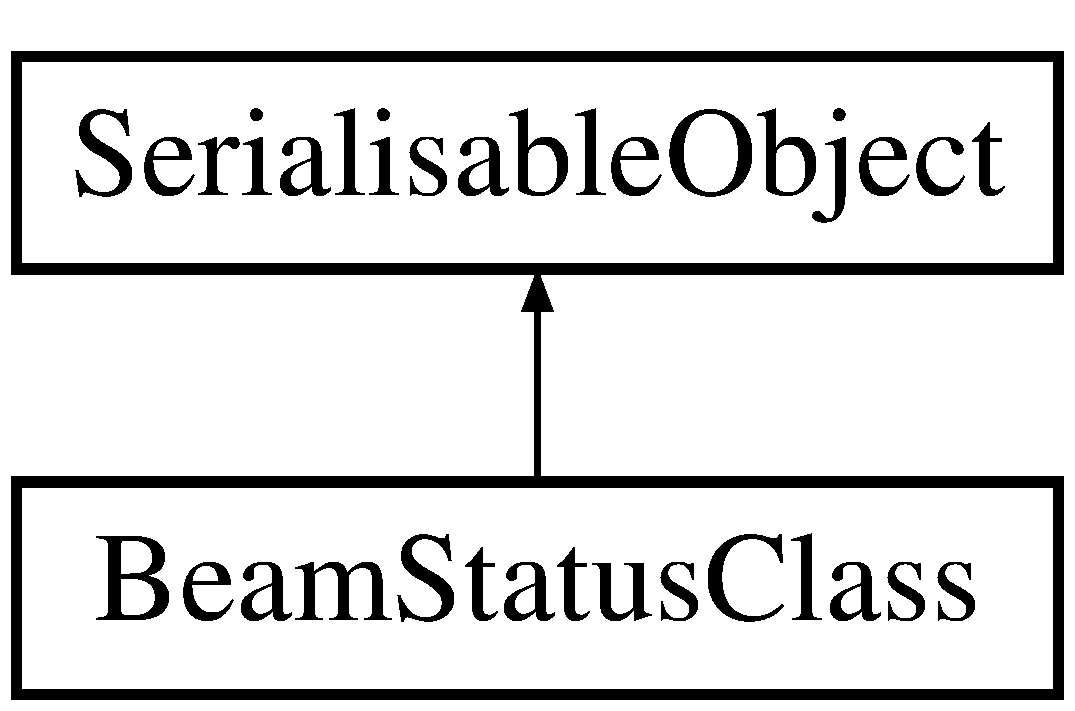
\includegraphics[height=2.000000cm]{classBeamStatusClass}
\end{center}
\end{figure}
\subsection*{Public Member Functions}
\begin{DoxyCompactItemize}
\item 
\hypertarget{classBeamStatusClass_a16f64e35b4c0c7fb4565b930393cf0dc}{{\bfseries Beam\-Status\-Class} (\hyperlink{classTimeClass}{Time\-Class} ts, double beaminten, double beampow, std\-::string beamstab)}\label{classBeamStatusClass_a16f64e35b4c0c7fb4565b930393cf0dc}

\item 
\hypertarget{classBeamStatusClass_a3099faed7d12197a62ee27dacee0d32d}{\hyperlink{classTimeClass}{Time\-Class} {\bfseries Get\-Timestamp} ()}\label{classBeamStatusClass_a3099faed7d12197a62ee27dacee0d32d}

\item 
\hypertarget{classBeamStatusClass_aee60c7ca2561a801cb80d6c239ca2189}{double {\bfseries Get\-Intensity} ()}\label{classBeamStatusClass_aee60c7ca2561a801cb80d6c239ca2189}

\item 
\hypertarget{classBeamStatusClass_abf408e07c997e60b084dc613d5fda75c}{double {\bfseries Get\-Power} ()}\label{classBeamStatusClass_abf408e07c997e60b084dc613d5fda75c}

\item 
\hypertarget{classBeamStatusClass_a052d6ca339a0ca531de200a6cb790fad}{std\-::string {\bfseries Get\-Stability} ()}\label{classBeamStatusClass_a052d6ca339a0ca531de200a6cb790fad}

\item 
\hypertarget{classBeamStatusClass_a26f08683ffd71565d38714886b130459}{void {\bfseries Set\-Timestamp} (\hyperlink{classTimeClass}{Time\-Class} Timestamp\-In)}\label{classBeamStatusClass_a26f08683ffd71565d38714886b130459}

\item 
\hypertarget{classBeamStatusClass_a6ad6d7fe6847a45a043115f6b452ce4a}{void {\bfseries Set\-Intensity} (double Intensity\-In)}\label{classBeamStatusClass_a6ad6d7fe6847a45a043115f6b452ce4a}

\item 
\hypertarget{classBeamStatusClass_a93db8cf0576994acb051c0c17d714e13}{void {\bfseries Set\-Power} (double Power\-In)}\label{classBeamStatusClass_a93db8cf0576994acb051c0c17d714e13}

\item 
\hypertarget{classBeamStatusClass_a4bae86f8f8d6ab9b74dbe73f456a97c6}{void {\bfseries Set\-Stability} (std\-::string Stability\-In)}\label{classBeamStatusClass_a4bae86f8f8d6ab9b74dbe73f456a97c6}

\item 
\hypertarget{classBeamStatusClass_a5a45cde713baaa1d205b0311c7a3ec23}{bool {\bfseries Print} ()}\label{classBeamStatusClass_a5a45cde713baaa1d205b0311c7a3ec23}

\item 
\hypertarget{classBeamStatusClass_a8b86d3c481eab24e6c8a2fda5940d7d8}{void {\bfseries Clear} ()}\label{classBeamStatusClass_a8b86d3c481eab24e6c8a2fda5940d7d8}

\end{DoxyCompactItemize}
\subsection*{Friends}
\begin{DoxyCompactItemize}
\item 
\hypertarget{classBeamStatusClass_ac98d07dd8f7b70e16ccb9a01abf56b9c}{class {\bfseries boost\-::serialization\-::access}}\label{classBeamStatusClass_ac98d07dd8f7b70e16ccb9a01abf56b9c}

\end{DoxyCompactItemize}


The documentation for this class was generated from the following file\-:\begin{DoxyCompactItemize}
\item 
Data\-Model/Beam\-Status\-Class.\-h\end{DoxyCompactItemize}

\hypertarget{classBeamTimeAna}{\section{Beam\-Time\-Ana Class Reference}
\label{classBeamTimeAna}\index{Beam\-Time\-Ana@{Beam\-Time\-Ana}}
}
Inheritance diagram for Beam\-Time\-Ana\-:\begin{figure}[H]
\begin{center}
\leavevmode
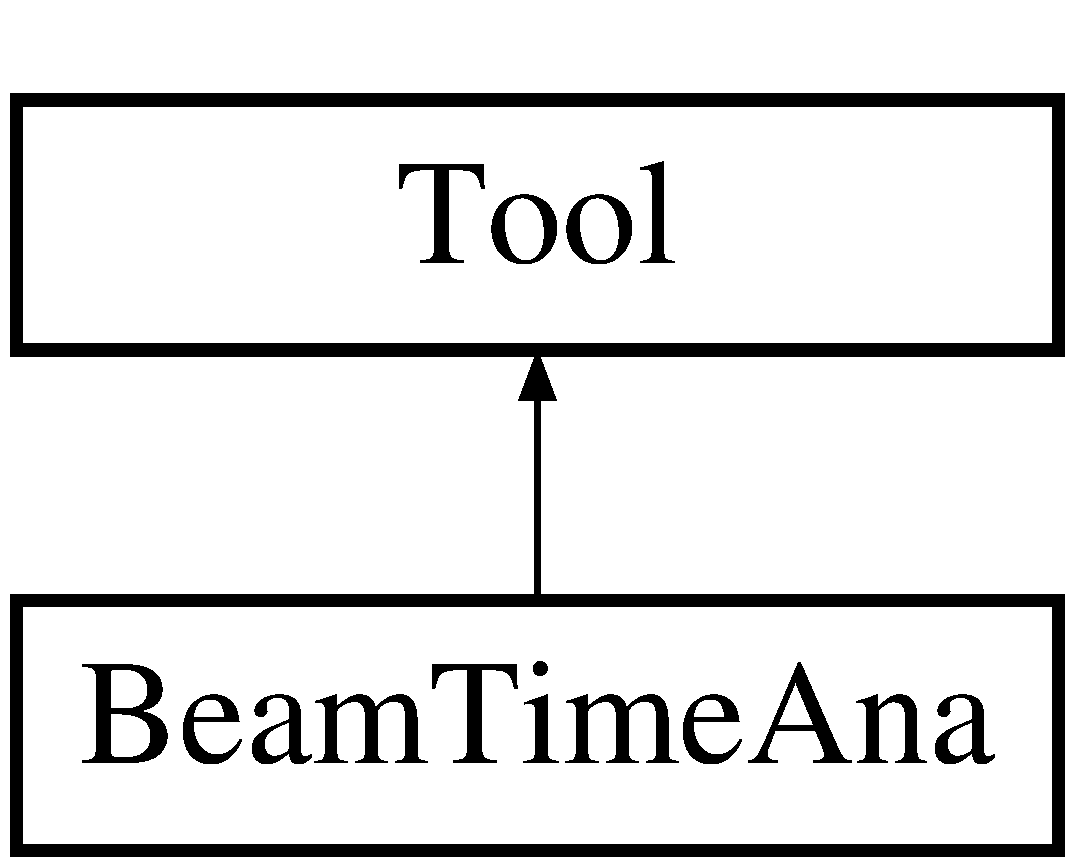
\includegraphics[height=2.000000cm]{classBeamTimeAna}
\end{center}
\end{figure}
\subsection*{Public Member Functions}
\begin{DoxyCompactItemize}
\item 
\hypertarget{classBeamTimeAna_ac5cfa1bfcae38f8b06e35165c34bc7a1}{bool {\bfseries Initialise} (std\-::string configfile, \hyperlink{classDataModel}{Data\-Model} \&data)}\label{classBeamTimeAna_ac5cfa1bfcae38f8b06e35165c34bc7a1}

\item 
\hypertarget{classBeamTimeAna_a7b308e1c38e71d712f86134f32d6f608}{bool {\bfseries Execute} ()}\label{classBeamTimeAna_a7b308e1c38e71d712f86134f32d6f608}

\item 
\hypertarget{classBeamTimeAna_a6327c7597f973dc8d379bab637d49158}{bool {\bfseries Finalise} ()}\label{classBeamTimeAna_a6327c7597f973dc8d379bab637d49158}

\item 
\hypertarget{classBeamTimeAna_a7371db48a169030dc1f3c4aef1d2118f}{vector$<$ double $>$ {\bfseries Transit} (double x0, double y0, double z0, double xslope, double yslope, double baseline, double radius)}\label{classBeamTimeAna_a7371db48a169030dc1f3c4aef1d2118f}

\end{DoxyCompactItemize}
\subsection*{Public Attributes}
\begin{DoxyCompactItemize}
\item 
\hypertarget{classBeamTimeAna_ab54934df684d5d4710b12eda9f0aa673}{T\-H1\-D $\ast$ {\bfseries hntp}}\label{classBeamTimeAna_ab54934df684d5d4710b12eda9f0aa673}

\item 
\hypertarget{classBeamTimeAna_a5faa850b2c2878a9b775ce3f4c709b42}{T\-H1\-D $\ast$ {\bfseries hbt}}\label{classBeamTimeAna_a5faa850b2c2878a9b775ce3f4c709b42}

\item 
\hypertarget{classBeamTimeAna_ab2dd35961bb27797a4611ec1b2893a6d}{T\-H1\-D $\ast$ {\bfseries hb\-E0}}\label{classBeamTimeAna_ab2dd35961bb27797a4611ec1b2893a6d}

\item 
\hypertarget{classBeamTimeAna_a6f771c25678b8227977259efd4885b55}{T\-H1\-D $\ast$ {\bfseries hb\-E\-\_\-early}}\label{classBeamTimeAna_a6f771c25678b8227977259efd4885b55}

\item 
\hypertarget{classBeamTimeAna_a9023b54b5567808d2255d05dd77914b9}{T\-H1\-D $\ast$ {\bfseries hb\-E\-\_\-med}}\label{classBeamTimeAna_a9023b54b5567808d2255d05dd77914b9}

\item 
\hypertarget{classBeamTimeAna_aa0db44ef40c14157b9722df4cb1fb200}{T\-H1\-D $\ast$ {\bfseries hb\-E\-\_\-late}}\label{classBeamTimeAna_aa0db44ef40c14157b9722df4cb1fb200}

\item 
\hypertarget{classBeamTimeAna_a19dc31c89cc2c1b4a80631fda8a8c363}{T\-H1\-D $\ast$ {\bfseries hbz0}}\label{classBeamTimeAna_a19dc31c89cc2c1b4a80631fda8a8c363}

\item 
\hypertarget{classBeamTimeAna_a4634c0e3b22b118c1254f59549046845}{T\-H1\-D $\ast$ {\bfseries hbbaseline}}\label{classBeamTimeAna_a4634c0e3b22b118c1254f59549046845}

\item 
\hypertarget{classBeamTimeAna_a727d2211d84e0683c805a7d98f0abc0a}{T\-H2\-D $\ast$ {\bfseries hbdvstimecorr}}\label{classBeamTimeAna_a727d2211d84e0683c805a7d98f0abc0a}

\item 
\hypertarget{classBeamTimeAna_af380e062647bdae7529b0d3f91c5a81d}{T\-String {\bfseries In\-File}}\label{classBeamTimeAna_af380e062647bdae7529b0d3f91c5a81d}

\item 
\hypertarget{classBeamTimeAna_a4d2aeab4e93fc15010e6fd1bf56edcdb}{T\-String {\bfseries Out\-File}}\label{classBeamTimeAna_a4d2aeab4e93fc15010e6fd1bf56edcdb}

\item 
\hypertarget{classBeamTimeAna_aaf94fd2c4bae8719cb3e40a467d427cd}{double {\bfseries target\-R}}\label{classBeamTimeAna_aaf94fd2c4bae8719cb3e40a467d427cd}

\item 
\hypertarget{classBeamTimeAna_a0df7b44ed1be5e0f23c6384dc09b01ca}{double {\bfseries baseline}}\label{classBeamTimeAna_a0df7b44ed1be5e0f23c6384dc09b01ca}

\item 
\hypertarget{classBeamTimeAna_ac21d70b3320574398e3251092f2c7ef5}{double {\bfseries tc1}}\label{classBeamTimeAna_ac21d70b3320574398e3251092f2c7ef5}

\item 
\hypertarget{classBeamTimeAna_ac3ff88abf8e308b8fad48bf1a994f530}{double {\bfseries tc2}}\label{classBeamTimeAna_ac3ff88abf8e308b8fad48bf1a994f530}

\item 
\hypertarget{classBeamTimeAna_a64a9f3610a0412a83b6f090e1622ef79}{double {\bfseries tc3}}\label{classBeamTimeAna_a64a9f3610a0412a83b6f090e1622ef79}

\item 
\hypertarget{classBeamTimeAna_a9fc48b9d0c43a1d696139811d15ba3c7}{int {\bfseries ientry}}\label{classBeamTimeAna_a9fc48b9d0c43a1d696139811d15ba3c7}

\end{DoxyCompactItemize}


The documentation for this class was generated from the following files\-:\begin{DoxyCompactItemize}
\item 
User\-Tools/\-Beam\-Time\-Ana/Beam\-Time\-Ana.\-h\item 
User\-Tools/\-Beam\-Time\-Ana/Beam\-Time\-Ana.\-cpp\end{DoxyCompactItemize}

\hypertarget{classBeamTimeTreeMaker}{\section{Beam\-Time\-Tree\-Maker Class Reference}
\label{classBeamTimeTreeMaker}\index{Beam\-Time\-Tree\-Maker@{Beam\-Time\-Tree\-Maker}}
}
Inheritance diagram for Beam\-Time\-Tree\-Maker\-:\begin{figure}[H]
\begin{center}
\leavevmode
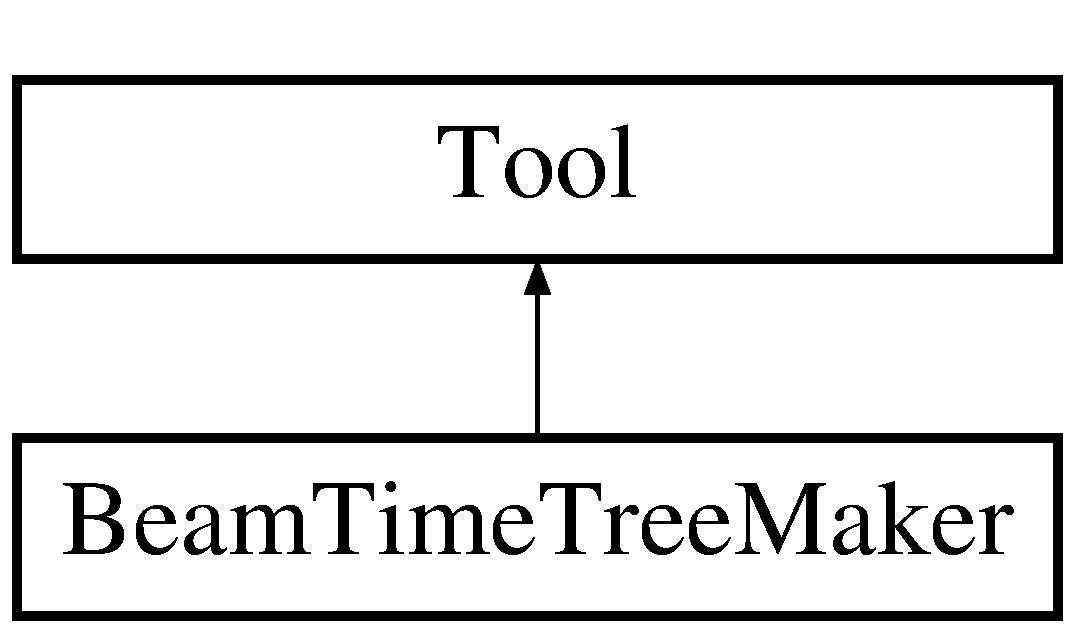
\includegraphics[height=2.000000cm]{classBeamTimeTreeMaker}
\end{center}
\end{figure}
\subsection*{Public Member Functions}
\begin{DoxyCompactItemize}
\item 
\hypertarget{classBeamTimeTreeMaker_ad0ff2ecf3cf282fc854c086f2bd6902e}{bool {\bfseries Initialise} (std\-::string configfile, \hyperlink{classDataModel}{Data\-Model} \&data)}\label{classBeamTimeTreeMaker_ad0ff2ecf3cf282fc854c086f2bd6902e}

\item 
\hypertarget{classBeamTimeTreeMaker_a9d8457a840bbd05785c6dbad41efc3e9}{bool {\bfseries Execute} ()}\label{classBeamTimeTreeMaker_a9d8457a840bbd05785c6dbad41efc3e9}

\item 
\hypertarget{classBeamTimeTreeMaker_aa854478ff70ed002e41ed38e18fe4a25}{bool {\bfseries Finalise} ()}\label{classBeamTimeTreeMaker_aa854478ff70ed002e41ed38e18fe4a25}

\end{DoxyCompactItemize}


The documentation for this class was generated from the following files\-:\begin{DoxyCompactItemize}
\item 
User\-Tools/\-Beam\-Time\-Tree\-Maker/Beam\-Time\-Tree\-Maker.\-h\item 
User\-Tools/\-Beam\-Time\-Tree\-Maker/Beam\-Time\-Tree\-Maker.\-cpp\end{DoxyCompactItemize}

\hypertarget{classBeamTimeTreeReader}{\section{Beam\-Time\-Tree\-Reader Class Reference}
\label{classBeamTimeTreeReader}\index{Beam\-Time\-Tree\-Reader@{Beam\-Time\-Tree\-Reader}}
}
Inheritance diagram for Beam\-Time\-Tree\-Reader\-:\begin{figure}[H]
\begin{center}
\leavevmode
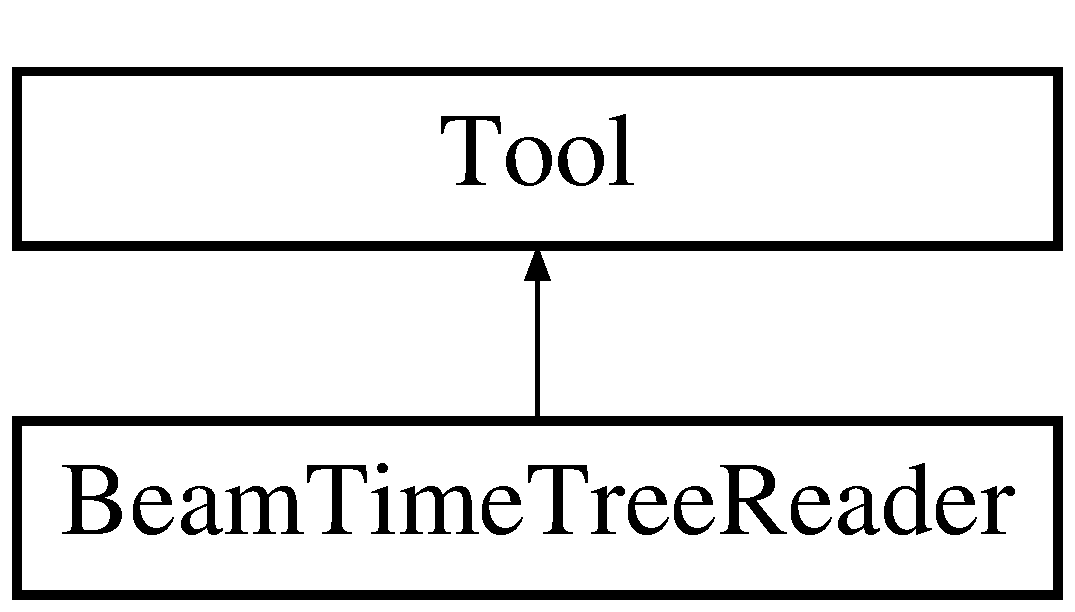
\includegraphics[height=2.000000cm]{classBeamTimeTreeReader}
\end{center}
\end{figure}
\subsection*{Public Member Functions}
\begin{DoxyCompactItemize}
\item 
\hypertarget{classBeamTimeTreeReader_a156a2386c5a9e9a6aab28a4fbf6df659}{bool {\bfseries Initialise} (std\-::string configfile, \hyperlink{classDataModel}{Data\-Model} \&data)}\label{classBeamTimeTreeReader_a156a2386c5a9e9a6aab28a4fbf6df659}

\item 
\hypertarget{classBeamTimeTreeReader_ae9094c6a47c9baa1a2394c50daa4fdb3}{bool {\bfseries Execute} ()}\label{classBeamTimeTreeReader_ae9094c6a47c9baa1a2394c50daa4fdb3}

\item 
\hypertarget{classBeamTimeTreeReader_ad6b505e7513ac9ab5b950cb15095ac79}{bool {\bfseries Finalise} ()}\label{classBeamTimeTreeReader_ad6b505e7513ac9ab5b950cb15095ac79}

\end{DoxyCompactItemize}


The documentation for this class was generated from the following files\-:\begin{DoxyCompactItemize}
\item 
User\-Tools/\-Beam\-Time\-Tree\-Reader/Beam\-Time\-Tree\-Reader.\-h\item 
User\-Tools/\-Beam\-Time\-Tree\-Reader/Beam\-Time\-Tree\-Reader.\-cpp\end{DoxyCompactItemize}

\hypertarget{classCalibratedADCWaveform}{
\section{CalibratedADCWaveform$<$ T $>$ Class Template Reference}
\label{classCalibratedADCWaveform}\index{CalibratedADCWaveform@{CalibratedADCWaveform}}
}
Inheritance diagram for CalibratedADCWaveform$<$ T $>$::\begin{figure}[H]
\begin{center}
\leavevmode
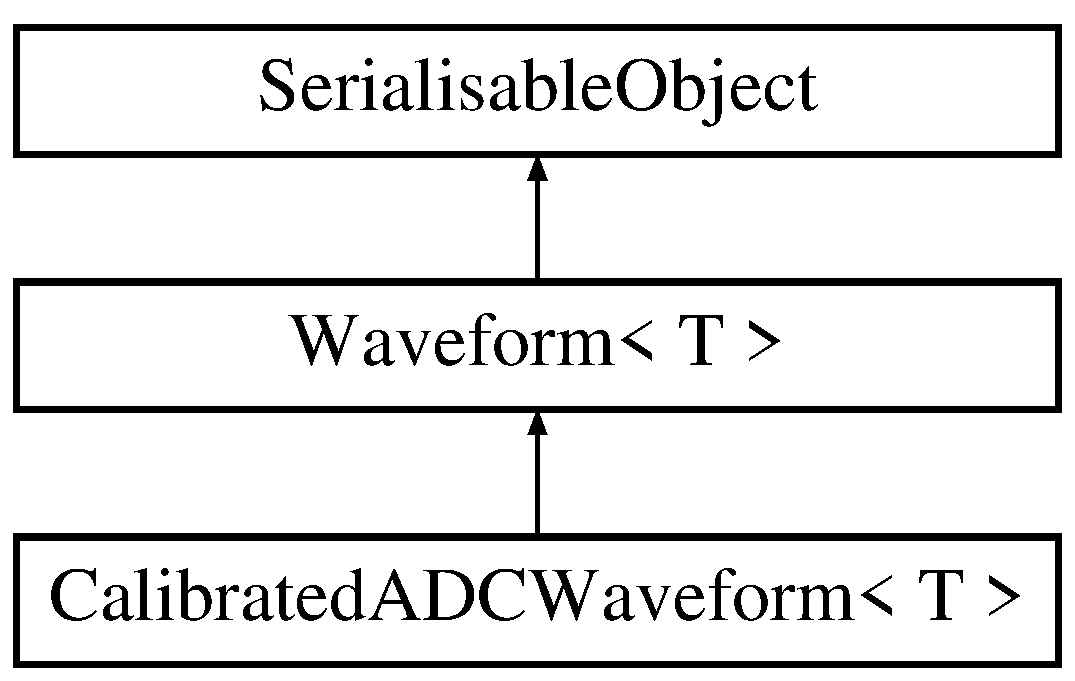
\includegraphics[height=3cm]{classCalibratedADCWaveform}
\end{center}
\end{figure}
\subsection*{Public Member Functions}
\begin{DoxyCompactItemize}
\item 
\hypertarget{classCalibratedADCWaveform_ab8d6abbf935c75db5de184c5a3291ef6}{
{\bfseries CalibratedADCWaveform} (const double \&tc, const std::vector$<$ T $>$ \&samples, double baseline, double sigma\_\-bl)}
\label{classCalibratedADCWaveform_ab8d6abbf935c75db5de184c5a3291ef6}

\item 
\hypertarget{classCalibratedADCWaveform_ae22d006546a5666eafd89d361a470798}{
double {\bfseries GetBaseline} () const }
\label{classCalibratedADCWaveform_ae22d006546a5666eafd89d361a470798}

\item 
\hypertarget{classCalibratedADCWaveform_a5afc74fd628dd6d70d60378467092e9d}{
double {\bfseries GetSigmaBaseline} () const }
\label{classCalibratedADCWaveform_a5afc74fd628dd6d70d60378467092e9d}

\end{DoxyCompactItemize}
\subsection*{Protected Member Functions}
\begin{DoxyCompactItemize}
\item 
\hypertarget{classCalibratedADCWaveform_a79b70f364816b8e558ab18d279b6b806}{
{\footnotesize template$<$class Archive $>$ }\\void {\bfseries serialize} (Archive \&ar, const unsigned int version)}
\label{classCalibratedADCWaveform_a79b70f364816b8e558ab18d279b6b806}

\end{DoxyCompactItemize}
\subsection*{Protected Attributes}
\begin{DoxyCompactItemize}
\item 
\hypertarget{classCalibratedADCWaveform_a149f3756091ef8101f03db1740db9caf}{
double \hyperlink{classCalibratedADCWaveform_a149f3756091ef8101f03db1740db9caf}{fBaseline}}
\label{classCalibratedADCWaveform_a149f3756091ef8101f03db1740db9caf}

\begin{DoxyCompactList}\small\item\em Estimated baseline (ADC counts) determined when performing the calibration. \item\end{DoxyCompactList}\item 
\hypertarget{classCalibratedADCWaveform_afad42e8ea016aa63d12da79d99b9a40c}{
double \hyperlink{classCalibratedADCWaveform_afad42e8ea016aa63d12da79d99b9a40c}{fSigmaBaseline}}
\label{classCalibratedADCWaveform_afad42e8ea016aa63d12da79d99b9a40c}

\begin{DoxyCompactList}\small\item\em Uncertainty (standard deviation) of the estimated baseline (ADC counts). \item\end{DoxyCompactList}\end{DoxyCompactItemize}
\subsection*{Friends}
\begin{DoxyCompactItemize}
\item 
\hypertarget{classCalibratedADCWaveform_ac98d07dd8f7b70e16ccb9a01abf56b9c}{
class {\bfseries boost::serialization::access}}
\label{classCalibratedADCWaveform_ac98d07dd8f7b70e16ccb9a01abf56b9c}

\end{DoxyCompactItemize}
\subsubsection*{template$<$typename T$>$ class CalibratedADCWaveform$<$ T $>$}



The documentation for this class was generated from the following file:\begin{DoxyCompactItemize}
\item 
DataModel/CalibratedADCWaveform.h\end{DoxyCompactItemize}

\hypertarget{classCardData}{
\section{CardData Class Reference}
\label{classCardData}\index{CardData@{CardData}}
}
\subsection*{Public Member Functions}
\begin{DoxyCompactItemize}
\item 
\hypertarget{classCardData_a77c665bfd5e8b1f17d6b668e888cf9bd}{
void {\bfseries Reset} ()}
\label{classCardData_a77c665bfd5e8b1f17d6b668e888cf9bd}

\end{DoxyCompactItemize}
\subsection*{Public Attributes}
\begin{DoxyCompactItemize}
\item 
\hypertarget{classCardData_a68649c499d7610955e7a9b143142e224}{
uint64\_\-t {\bfseries LastSync}}
\label{classCardData_a68649c499d7610955e7a9b143142e224}

\item 
\hypertarget{classCardData_a4fdf5313faebd27fee17096a31d0e28e}{
int {\bfseries SequenceID}}
\label{classCardData_a4fdf5313faebd27fee17096a31d0e28e}

\item 
\hypertarget{classCardData_a1297c0ccdeb5cb134cef3c92e01a36ed}{
int {\bfseries StartTimeSec}}
\label{classCardData_a1297c0ccdeb5cb134cef3c92e01a36ed}

\item 
\hypertarget{classCardData_af5393836942c9d857039e8b11bac2952}{
int {\bfseries StartTimeNSec}}
\label{classCardData_af5393836942c9d857039e8b11bac2952}

\item 
\hypertarget{classCardData_a7bd1f3c2269b6c7d3f12ffdd59efa1e6}{
uint64\_\-t {\bfseries StartCount}}
\label{classCardData_a7bd1f3c2269b6c7d3f12ffdd59efa1e6}

\item 
\hypertarget{classCardData_a816053ce45a07b8f7a7e5bfd914c51db}{
std::vector$<$ ULong64\_\-t $>$ {\bfseries TriggerCounts}}
\label{classCardData_a816053ce45a07b8f7a7e5bfd914c51db}

\item 
\hypertarget{classCardData_ab44adb08a1c2de7f4d24463325c87934}{
std::vector$<$ UInt\_\-t $>$ {\bfseries Rates}}
\label{classCardData_ab44adb08a1c2de7f4d24463325c87934}

\item 
\hypertarget{classCardData_a36cb9c0f73fcf5eae251e0a2b1b2bd0f}{
int {\bfseries CardID}}
\label{classCardData_a36cb9c0f73fcf5eae251e0a2b1b2bd0f}

\item 
\hypertarget{classCardData_a6307217de93243eb7b0aa9931f02f706}{
int {\bfseries TriggerNumber}}
\label{classCardData_a6307217de93243eb7b0aa9931f02f706}

\item 
\hypertarget{classCardData_a98f397c0dd49007942f5f25c8cbc67f0}{
int {\bfseries Channels}}
\label{classCardData_a98f397c0dd49007942f5f25c8cbc67f0}

\item 
\hypertarget{classCardData_a82c5fd806c6529cf7a9625dc262f9e8d}{
int {\bfseries BufferSize}}
\label{classCardData_a82c5fd806c6529cf7a9625dc262f9e8d}

\item 
\hypertarget{classCardData_abafe428221ab0987ac51bd7312b29d6b}{
int {\bfseries Eventsize}}
\label{classCardData_abafe428221ab0987ac51bd7312b29d6b}

\item 
\hypertarget{classCardData_a3395d60095ef7aeff93cf2d169a34395}{
int {\bfseries FullBufferSize}}
\label{classCardData_a3395d60095ef7aeff93cf2d169a34395}

\item 
\hypertarget{classCardData_a6190a518c1cc009d169a0f94a333576d}{
std::vector$<$ uint16\_\-t $>$ {\bfseries Data}}
\label{classCardData_a6190a518c1cc009d169a0f94a333576d}

\end{DoxyCompactItemize}


The documentation for this class was generated from the following files:\begin{DoxyCompactItemize}
\item 
UserTools/PulseSimulation/CardData.h\item 
UserTools/PulseSimulation/CardData.cpp\end{DoxyCompactItemize}

\hypertarget{classChannel}{\section{Channel Class Reference}
\label{classChannel}\index{Channel@{Channel}}
}
Inheritance diagram for Channel\-:\begin{figure}[H]
\begin{center}
\leavevmode
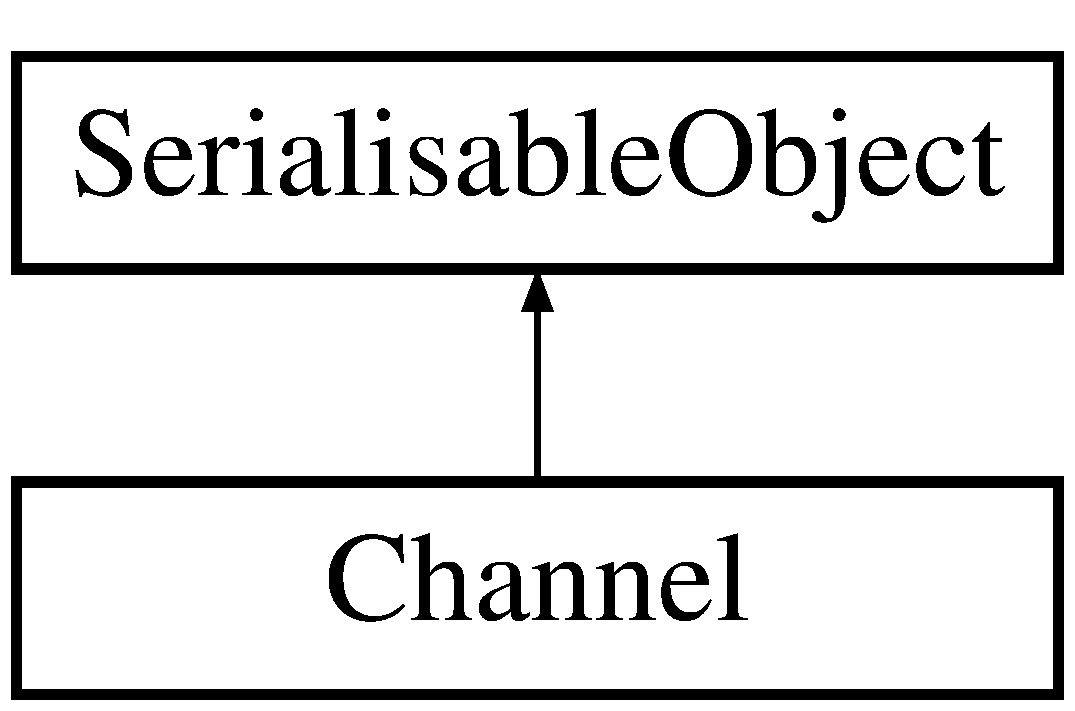
\includegraphics[height=2.000000cm]{classChannel}
\end{center}
\end{figure}
\subsection*{Public Member Functions}
\begin{DoxyCompactItemize}
\item 
\hypertarget{classChannel_ae1078b5c2230dd8fcba2bbd4e8100c57}{{\bfseries Channel} (unsigned long chn\-I\-D, \hyperlink{classPosition}{Position} chanpos, int strp, int strpnm, unsigned int sig\-\_\-crt, unsigned int sig\-\_\-crd, unsigned int sig\-\_\-chn, unsigned int lv2\-\_\-crt, unsigned int lv2\-\_\-crd, unsigned int lv2\-\_\-ch, unsigned int hv\-\_\-crt, unsigned int hv\-\_\-crd, unsigned int hv\-\_\-chn, channelstatus chanstat)}\label{classChannel_ae1078b5c2230dd8fcba2bbd4e8100c57}

\item 
\hypertarget{classChannel_a135981325d6cd967c06b27eef9f0abb0}{unsigned long {\bfseries Get\-Channel\-I\-D} ()}\label{classChannel_a135981325d6cd967c06b27eef9f0abb0}

\item 
\hypertarget{classChannel_a20f0f3be320a2bb029169a4dbe93cf90}{\hyperlink{classPosition}{Position} {\bfseries Get\-Channel\-Position} ()}\label{classChannel_a20f0f3be320a2bb029169a4dbe93cf90}

\item 
\hypertarget{classChannel_aaf73be7554bca0d37886ead17e7dd378}{int {\bfseries Get\-Strip\-Side} ()}\label{classChannel_aaf73be7554bca0d37886ead17e7dd378}

\item 
\hypertarget{classChannel_a8e11f287e50dd85bc16ec31cab5b19f5}{int {\bfseries Get\-Strip\-Num} ()}\label{classChannel_a8e11f287e50dd85bc16ec31cab5b19f5}

\item 
\hypertarget{classChannel_a75f4e595dfd853b4705aaab4b4dd7e5d}{unsigned int {\bfseries Get\-Signal\-Crate} ()}\label{classChannel_a75f4e595dfd853b4705aaab4b4dd7e5d}

\item 
\hypertarget{classChannel_a3fe69d8eb34bbb71101faa490eff401c}{unsigned int {\bfseries Get\-Signal\-Card} ()}\label{classChannel_a3fe69d8eb34bbb71101faa490eff401c}

\item 
\hypertarget{classChannel_a0adb3da425cdc8571e3f2070339d1b45}{unsigned int {\bfseries Get\-Signal\-Channel} ()}\label{classChannel_a0adb3da425cdc8571e3f2070339d1b45}

\item 
\hypertarget{classChannel_aed336de8cbfe7b004a966b08998f10a1}{unsigned int {\bfseries Get\-Level2\-Crate} ()}\label{classChannel_aed336de8cbfe7b004a966b08998f10a1}

\item 
\hypertarget{classChannel_a8664e03b00cfb5d9089ffc730ad2db8a}{unsigned int {\bfseries Get\-Level2\-Card} ()}\label{classChannel_a8664e03b00cfb5d9089ffc730ad2db8a}

\item 
\hypertarget{classChannel_a3d15a263e8282224e6cac3e39fc537e2}{unsigned int {\bfseries Get\-Level2\-Channel} ()}\label{classChannel_a3d15a263e8282224e6cac3e39fc537e2}

\item 
\hypertarget{classChannel_a976eb5f1f568d25d7e6581e947c9026a}{unsigned int {\bfseries Get\-Hv\-Crate} ()}\label{classChannel_a976eb5f1f568d25d7e6581e947c9026a}

\item 
\hypertarget{classChannel_a77afff8e584d72b11c326d503af8cf31}{unsigned int {\bfseries Get\-Hv\-Card} ()}\label{classChannel_a77afff8e584d72b11c326d503af8cf31}

\item 
\hypertarget{classChannel_ab0be6e53cc497a9adfd07d117bd1b8a6}{unsigned int {\bfseries Get\-Hv\-Channel} ()}\label{classChannel_ab0be6e53cc497a9adfd07d117bd1b8a6}

\item 
\hypertarget{classChannel_a0de7daf81b2cf2931ad002365b4e83a7}{channelstatus {\bfseries Get\-Status} ()}\label{classChannel_a0de7daf81b2cf2931ad002365b4e83a7}

\item 
\hypertarget{classChannel_abc8868d1474907bf055649280aee6ee9}{void {\bfseries Set\-Channel\-I\-D} (unsigned long channel\-I\-Din)}\label{classChannel_abc8868d1474907bf055649280aee6ee9}

\item 
\hypertarget{classChannel_a1ce153da74e56914bfe92f1300d9c4db}{void {\bfseries Set\-Rel\-Pos} (\hyperlink{classPosition}{Position} pos)}\label{classChannel_a1ce153da74e56914bfe92f1300d9c4db}

\item 
\hypertarget{classChannel_a2e0a7f64af8639f223be6ae34ee1c866}{void {\bfseries Set\-Strip\-Side} (int stripsidein)}\label{classChannel_a2e0a7f64af8639f223be6ae34ee1c866}

\item 
\hypertarget{classChannel_a1f6b1314cb1db51fd36ed6a734d46af8}{void {\bfseries Set\-Strip\-Num} (int stripnumin)}\label{classChannel_a1f6b1314cb1db51fd36ed6a734d46af8}

\item 
\hypertarget{classChannel_ac7c8bc08322263962606adcee41e5fb9}{void {\bfseries Set\-Signal\-Crate} (unsigned int cratein)}\label{classChannel_ac7c8bc08322263962606adcee41e5fb9}

\item 
\hypertarget{classChannel_aaa842caa030e691f361bbb38b60c19ac}{void {\bfseries Set\-Signal\-Card} (unsigned int cardin)}\label{classChannel_aaa842caa030e691f361bbb38b60c19ac}

\item 
\hypertarget{classChannel_acd431f017fca170ea3036f96b0f79e9f}{void {\bfseries Set\-Signal\-Channel} (unsigned int chanin)}\label{classChannel_acd431f017fca170ea3036f96b0f79e9f}

\item 
\hypertarget{classChannel_a82c97b5b03f81dc4c415f9e6ff4e5cd7}{void {\bfseries Set\-Level2\-Crate} (unsigned int cratein)}\label{classChannel_a82c97b5b03f81dc4c415f9e6ff4e5cd7}

\item 
\hypertarget{classChannel_a7144068a386f201f596bb389a09c2806}{void {\bfseries Set\-Level2\-Card} (unsigned int cardin)}\label{classChannel_a7144068a386f201f596bb389a09c2806}

\item 
\hypertarget{classChannel_ab6fbf3a0ad9f0a81f57e78b4d0030b1b}{void {\bfseries Set\-Level2\-Channel} (unsigned int chanin)}\label{classChannel_ab6fbf3a0ad9f0a81f57e78b4d0030b1b}

\item 
\hypertarget{classChannel_a0fa53863af75dc3113462587216eb72f}{void {\bfseries Set\-Hv\-Crate} (unsigned int cratein)}\label{classChannel_a0fa53863af75dc3113462587216eb72f}

\item 
\hypertarget{classChannel_a6d80a27a7baf8c35f107794f3907cd8f}{void {\bfseries Set\-Hv\-Card} (unsigned int cardin)}\label{classChannel_a6d80a27a7baf8c35f107794f3907cd8f}

\item 
\hypertarget{classChannel_ab710af8a4a2334b2fecb7908ef14f18b}{void {\bfseries Set\-Hv\-Channel} (unsigned int chanin)}\label{classChannel_ab710af8a4a2334b2fecb7908ef14f18b}

\item 
\hypertarget{classChannel_af036686e0a7cecce9996e28cf7f2067f}{void {\bfseries Set\-Status} (channelstatus stat)}\label{classChannel_af036686e0a7cecce9996e28cf7f2067f}

\item 
\hypertarget{classChannel_a8361bdcaf6dfafc874f6a612dcded25a}{bool {\bfseries Print} ()}\label{classChannel_a8361bdcaf6dfafc874f6a612dcded25a}

\item 
\hypertarget{classChannel_ad5ceba06c660386cafaf7801f6adbfad}{bool {\bfseries Print\-Status} (channelstatus status)}\label{classChannel_ad5ceba06c660386cafaf7801f6adbfad}

\end{DoxyCompactItemize}
\subsection*{Friends}
\begin{DoxyCompactItemize}
\item 
\hypertarget{classChannel_ac98d07dd8f7b70e16ccb9a01abf56b9c}{class {\bfseries boost\-::serialization\-::access}}\label{classChannel_ac98d07dd8f7b70e16ccb9a01abf56b9c}

\end{DoxyCompactItemize}


The documentation for this class was generated from the following file\-:\begin{DoxyCompactItemize}
\item 
Data\-Model/Channel.\-h\end{DoxyCompactItemize}

\hypertarget{classChannelKey}{
\section{ChannelKey Class Reference}
\label{classChannelKey}\index{ChannelKey@{ChannelKey}}
}
Inheritance diagram for ChannelKey::\begin{figure}[H]
\begin{center}
\leavevmode
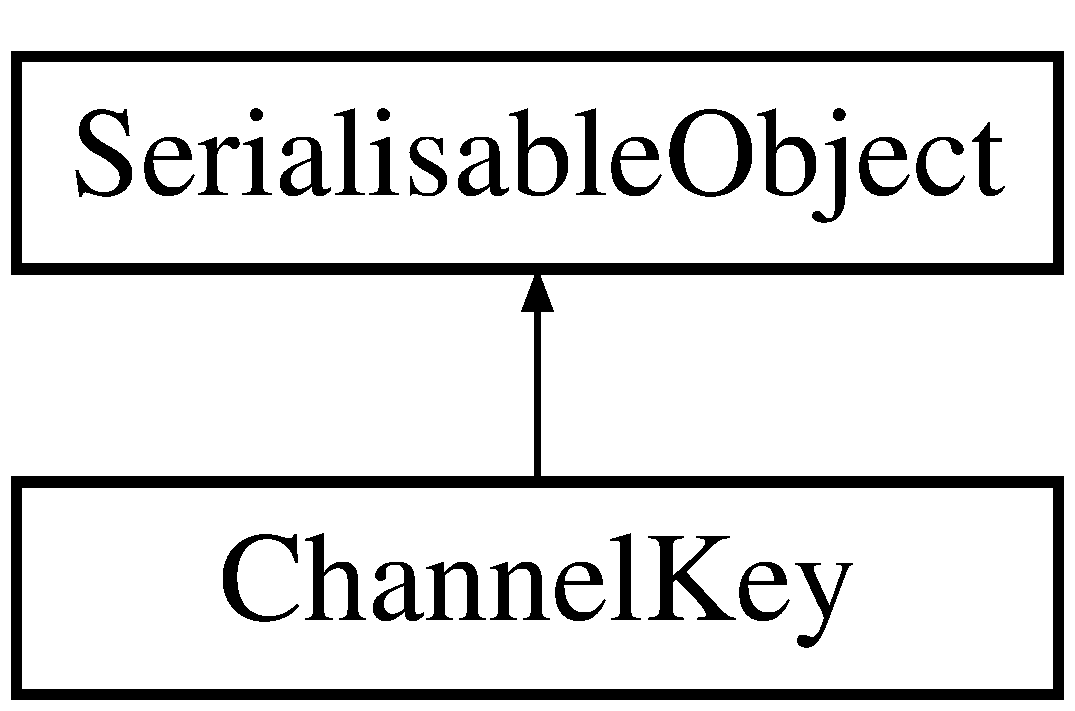
\includegraphics[height=2cm]{classChannelKey}
\end{center}
\end{figure}
\subsection*{Public Member Functions}
\begin{DoxyCompactItemize}
\item 
\hypertarget{classChannelKey_a1b98b5ec38b5a372908869bec5e76885}{
{\bfseries ChannelKey} (subdetector subdetin, uint32\_\-t detelin)}
\label{classChannelKey_a1b98b5ec38b5a372908869bec5e76885}

\item 
\hypertarget{classChannelKey_a5b156478be91e4d58829661e9a63da13}{
subdetector {\bfseries GetSubDetectorType} () const }
\label{classChannelKey_a5b156478be91e4d58829661e9a63da13}

\item 
\hypertarget{classChannelKey_a2788a95997db38d5bf8075da6eb2d50c}{
uint32\_\-t {\bfseries GetDetectorElementIndex} () const }
\label{classChannelKey_a2788a95997db38d5bf8075da6eb2d50c}

\item 
\hypertarget{classChannelKey_a84b468bc66e943e8ad9b4102f8c8446d}{
void {\bfseries SetSubDetectorType} (subdetector subdetin)}
\label{classChannelKey_a84b468bc66e943e8ad9b4102f8c8446d}

\item 
\hypertarget{classChannelKey_a8727334520a49cba3d6a01a6727a361d}{
void {\bfseries SetDetectorElementIndex} (uint32\_\-t detelin)}
\label{classChannelKey_a8727334520a49cba3d6a01a6727a361d}

\item 
\hypertarget{classChannelKey_a7bb14ec44da38dd1152cf7912f7a607d}{
bool {\bfseries Print} ()}
\label{classChannelKey_a7bb14ec44da38dd1152cf7912f7a607d}

\item 
\hypertarget{classChannelKey_abcadfaf457add635aef1ec372e5340d7}{
bool {\bfseries operator$<$} (const \hyperlink{classChannelKey}{ChannelKey} rhs) const }
\label{classChannelKey_abcadfaf457add635aef1ec372e5340d7}

\end{DoxyCompactItemize}
\subsection*{Friends}
\begin{DoxyCompactItemize}
\item 
\hypertarget{classChannelKey_ac98d07dd8f7b70e16ccb9a01abf56b9c}{
class {\bfseries boost::serialization::access}}
\label{classChannelKey_ac98d07dd8f7b70e16ccb9a01abf56b9c}

\end{DoxyCompactItemize}


The documentation for this class was generated from the following file:\begin{DoxyCompactItemize}
\item 
DataModel/ChannelKey.h\end{DoxyCompactItemize}

\hypertarget{classCheckDetectorCounts}{
\section{CheckDetectorCounts Class Reference}
\label{classCheckDetectorCounts}\index{CheckDetectorCounts@{CheckDetectorCounts}}
}
\subsection*{Public Member Functions}
\begin{DoxyCompactItemize}
\item 
\hypertarget{classCheckDetectorCounts_ac64b90d8952c7d3b1f970c7f7d6180df}{
bool {\bfseries Initialise} (std::string configfile, \hyperlink{classDataModel}{DataModel} \&data)}
\label{classCheckDetectorCounts_ac64b90d8952c7d3b1f970c7f7d6180df}

\item 
\hypertarget{classCheckDetectorCounts_a5e10b7af8ac4184d2cfc695b47e5c23d}{
bool {\bfseries Execute} ()}
\label{classCheckDetectorCounts_a5e10b7af8ac4184d2cfc695b47e5c23d}

\item 
\hypertarget{classCheckDetectorCounts_a7fb977a13d93552a7e7feefd9a419125}{
bool {\bfseries Finalise} ()}
\label{classCheckDetectorCounts_a7fb977a13d93552a7e7feefd9a419125}

\end{DoxyCompactItemize}


The documentation for this class was generated from the following files:\begin{DoxyCompactItemize}
\item 
UserTools/CheckDetectorCounts/CheckDetectorCounts.h\item 
UserTools/CheckDetectorCounts/CheckDetectorCounts.cpp\end{DoxyCompactItemize}

\hypertarget{classDataModel}{
\section{DataModel Class Reference}
\label{classDataModel}\index{DataModel@{DataModel}}
}


{\ttfamily \#include $<$DataModel.h$>$}\subsection*{Public Member Functions}
\begin{DoxyCompactItemize}
\item 
\hypertarget{classDataModel_abff03aef2cb531142a35781bb87c3365}{
\hyperlink{classDataModel_abff03aef2cb531142a35781bb87c3365}{DataModel} ()}
\label{classDataModel_abff03aef2cb531142a35781bb87c3365}

\begin{DoxyCompactList}\small\item\em Simple constructor. \item\end{DoxyCompactList}\end{DoxyCompactItemize}
\subsection*{Public Attributes}
\begin{DoxyCompactItemize}
\item 
\hypertarget{classDataModel_a4baac5fe364a7a23762d70d2c2216486}{
Store \hyperlink{classDataModel_a4baac5fe364a7a23762d70d2c2216486}{vars}}
\label{classDataModel_a4baac5fe364a7a23762d70d2c2216486}

\begin{DoxyCompactList}\small\item\em This Store can be used for any variables. It is an inefficent ascii based storage. \item\end{DoxyCompactList}\item 
\hypertarget{classDataModel_a878e0d87285f0b3541a3e7116a5f00b6}{
BoostStore \hyperlink{classDataModel_a878e0d87285f0b3541a3e7116a5f00b6}{CStore}}
\label{classDataModel_a878e0d87285f0b3541a3e7116a5f00b6}

\begin{DoxyCompactList}\small\item\em This is a more efficent binary BoostStore that can be used to store a dynamic set of inter Tool variables. \item\end{DoxyCompactList}\item 
\hypertarget{classDataModel_ad1ffc080c3b263bf3ee382a531321ad4}{
std::map$<$ std::string, BoostStore $\ast$ $>$ \hyperlink{classDataModel_ad1ffc080c3b263bf3ee382a531321ad4}{Stores}}
\label{classDataModel_ad1ffc080c3b263bf3ee382a531321ad4}

\begin{DoxyCompactList}\small\item\em This is a map of named BooStore pointers which can be deffined to hold a nammed collection of any tipe of BoostStore. It is usefull to store data that needs subdividing into differnt stores. \item\end{DoxyCompactList}\item 
\hypertarget{classDataModel_aa777da4c632e4659ee5b1447ad513458}{
Logging $\ast$ \hyperlink{classDataModel_aa777da4c632e4659ee5b1447ad513458}{Log}}
\label{classDataModel_aa777da4c632e4659ee5b1447ad513458}

\begin{DoxyCompactList}\small\item\em Log class pointer for use in Tools, it can be used to send messages which can have multiple error levels and destination end points. \item\end{DoxyCompactList}\item 
\hypertarget{classDataModel_a2c6dfd692e50f90e55338970ea7f8d61}{
zmq::context\_\-t $\ast$ \hyperlink{classDataModel_a2c6dfd692e50f90e55338970ea7f8d61}{context}}
\label{classDataModel_a2c6dfd692e50f90e55338970ea7f8d61}

\begin{DoxyCompactList}\small\item\em ZMQ contex used for producing zmq sockets for inter thread, process, or computer communication. \item\end{DoxyCompactList}\end{DoxyCompactItemize}


\subsection{Detailed Description}
This class Is a transient data model class for your Tools within the ToolChain. If Tools need to comunicate they pass all data objects through the data model. There fore inter tool data objects should be deffined in this class.

Author}
B.Richards Date}
2019/05/26 18:34:00 Contact: \href{mailto:b.richards@qmul.ac.uk}{\tt b.richards@qmul.ac.uk} 

The documentation for this class was generated from the following files:\begin{DoxyCompactItemize}
\item 
DataModel/DataModel.h\item 
DataModel/DataModel.cpp\end{DoxyCompactItemize}

\include{classdenseMatrix}
\hypertarget{classDetector}{\section{Detector Class Reference}
\label{classDetector}\index{Detector@{Detector}}
}
Inheritance diagram for Detector\-:\begin{figure}[H]
\begin{center}
\leavevmode
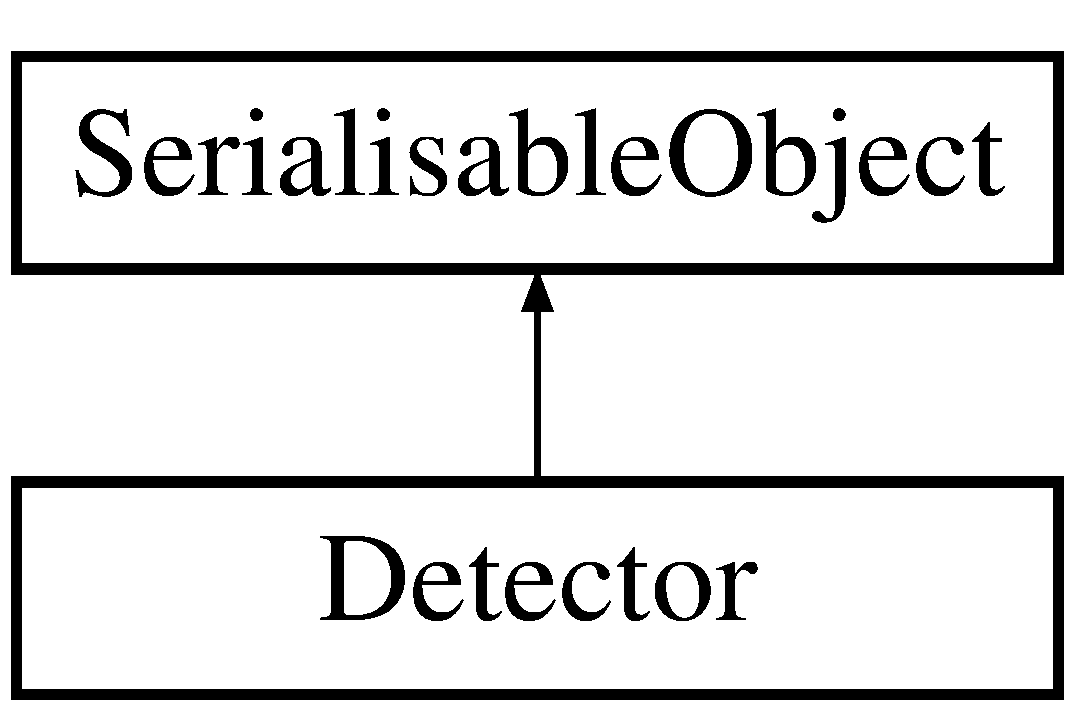
\includegraphics[height=2.000000cm]{classDetector}
\end{center}
\end{figure}
\subsection*{Public Member Functions}
\begin{DoxyCompactItemize}
\item 
\hypertarget{classDetector_acc63b0828ae0a8fecca2f71b26f14531}{{\bfseries Detector} (int detid, std\-::string Det\-Ele, std\-::string Cyl\-Loc, \hyperlink{classPosition}{Position} posin, \hyperlink{classDirection}{Direction} dirin, std\-::string detype, detectorstatus stat, double avgrate, map$<$ unsigned long, \hyperlink{classChannel}{Channel} $>$ channelsin=\{\})}\label{classDetector_acc63b0828ae0a8fecca2f71b26f14531}

\item 
\hypertarget{classDetector_a7622dcc0d32a77b2d81f3346f9d486a6}{std\-::string {\bfseries Get\-Detector\-Element} ()}\label{classDetector_a7622dcc0d32a77b2d81f3346f9d486a6}

\item 
\hypertarget{classDetector_ae706947ab25223c2707b0b04fa1cf999}{\hyperlink{classPosition}{Position} {\bfseries Get\-Detector\-Position} ()}\label{classDetector_ae706947ab25223c2707b0b04fa1cf999}

\item 
\hypertarget{classDetector_ace3843de946676dac6a031ab21ab2537}{\hyperlink{classPosition}{Position} {\bfseries Get\-Position\-In\-Tank} ()}\label{classDetector_ace3843de946676dac6a031ab21ab2537}

\item 
\hypertarget{classDetector_a80cbd9a7402579d601953a91d6883a94}{\hyperlink{classDirection}{Direction} {\bfseries Get\-Detector\-Direction} ()}\label{classDetector_a80cbd9a7402579d601953a91d6883a94}

\item 
\hypertarget{classDetector_a85412b023bb48b28e27c9b308857653f}{int {\bfseries Get\-Detector\-I\-D} ()}\label{classDetector_a85412b023bb48b28e27c9b308857653f}

\item 
\hypertarget{classDetector_a0f5e4f78e6e64903f46679577609a320}{std\-::string {\bfseries Get\-Detector\-Type} ()}\label{classDetector_a0f5e4f78e6e64903f46679577609a320}

\item 
\hypertarget{classDetector_adf81db079151a065407d44558a6240b3}{detectorstatus {\bfseries Get\-Status} ()}\label{classDetector_adf81db079151a065407d44558a6240b3}

\item 
\hypertarget{classDetector_a1aa42e2f99fd99f2b09d2ab0a1ff4405}{std\-::map$<$ unsigned long, \\*
\hyperlink{classChannel}{Channel} $>$ $\ast$ {\bfseries Get\-Channels} ()}\label{classDetector_a1aa42e2f99fd99f2b09d2ab0a1ff4405}

\item 
\hypertarget{classDetector_adc95528c7b20269f2f30a6d5330a7fd7}{void {\bfseries Add\-Channel} (\hyperlink{classChannel}{Channel} chanin)}\label{classDetector_adc95528c7b20269f2f30a6d5330a7fd7}

\item 
\hypertarget{classDetector_aa87b945be097376ed4d9e7ad11da60f5}{std\-::string {\bfseries Get\-Tank\-Location} ()}\label{classDetector_aa87b945be097376ed4d9e7ad11da60f5}

\item 
\hypertarget{classDetector_ac0b5f82030923f555f4420c110de97b0}{\hyperlink{classGeometry}{Geometry} $\ast$ {\bfseries Get\-Geometry\-Ptr} ()}\label{classDetector_ac0b5f82030923f555f4420c110de97b0}

\item 
\hypertarget{classDetector_a5a447c98e1cda4bcb669d6f0cf7f372e}{void {\bfseries Set\-Detector\-Element} (std\-::string Det\-Ele\-In)}\label{classDetector_a5a447c98e1cda4bcb669d6f0cf7f372e}

\item 
\hypertarget{classDetector_a388c07e8a741d22a5dcec27ae0718223}{void {\bfseries Set\-Detector\-Position} (\hyperlink{classPosition}{Position} Detector\-Position\-In)}\label{classDetector_a388c07e8a741d22a5dcec27ae0718223}

\item 
\hypertarget{classDetector_a349a08c4b6eb90415971d798f6c35466}{void {\bfseries Set\-Detector\-Direction} (\hyperlink{classDirection}{Direction} Detector\-Direction\-In)}\label{classDetector_a349a08c4b6eb90415971d798f6c35466}

\item 
\hypertarget{classDetector_ac6b4e26f7391b0e96cddf047aec6baf3}{void {\bfseries Set\-Detector\-I\-D} (int Detector\-I\-D\-In)}\label{classDetector_ac6b4e26f7391b0e96cddf047aec6baf3}

\item 
\hypertarget{classDetector_ac903797b8948e0107de513de60757b2e}{void {\bfseries Set\-Detector\-Type} (std\-::string Detector\-Type\-In)}\label{classDetector_ac903797b8948e0107de513de60757b2e}

\item 
\hypertarget{classDetector_a912c695a5b4c7bdac1fd6d408cb4e943}{void {\bfseries Set\-Status} (detectorstatus Status\-In)}\label{classDetector_a912c695a5b4c7bdac1fd6d408cb4e943}

\item 
\hypertarget{classDetector_acc18123ffd61248f94f86eae4a54a0af}{void {\bfseries Set\-Tank\-Location} (std\-::string locin)}\label{classDetector_acc18123ffd61248f94f86eae4a54a0af}

\item 
\hypertarget{classDetector_a314120e55ef11500f7e0463e94ae37bb}{void {\bfseries Set\-Geometry\-Ptr} (\hyperlink{classGeometry}{Geometry} $\ast$geomin)}\label{classDetector_a314120e55ef11500f7e0463e94ae37bb}

\item 
\hypertarget{classDetector_a89a77c0af830a448ab599e9cfce4a2d8}{bool {\bfseries Print} ()}\label{classDetector_a89a77c0af830a448ab599e9cfce4a2d8}

\item 
\hypertarget{classDetector_a4fced6fd118fe1371ee7e7193c666710}{bool {\bfseries Print\-Status} (detectorstatus status)}\label{classDetector_a4fced6fd118fe1371ee7e7193c666710}

\item 
\hypertarget{classDetector_af25e30e52b653b1380743676322f88ea}{void {\bfseries Print\-Channels} ()}\label{classDetector_af25e30e52b653b1380743676322f88ea}

\end{DoxyCompactItemize}
\subsection*{Friends}
\begin{DoxyCompactItemize}
\item 
\hypertarget{classDetector_ac98d07dd8f7b70e16ccb9a01abf56b9c}{class {\bfseries boost\-::serialization\-::access}}\label{classDetector_ac98d07dd8f7b70e16ccb9a01abf56b9c}

\end{DoxyCompactItemize}


The documentation for this class was generated from the following files\-:\begin{DoxyCompactItemize}
\item 
Data\-Model/Detector.\-h\item 
Data\-Model/Detector.\-cpp\end{DoxyCompactItemize}

\hypertarget{classDigitBuilder}{\section{Digit\-Builder Class Reference}
\label{classDigitBuilder}\index{Digit\-Builder@{Digit\-Builder}}
}


{\ttfamily \#include $<$Digit\-Builder.\-h$>$}

Inheritance diagram for Digit\-Builder\-:\begin{figure}[H]
\begin{center}
\leavevmode
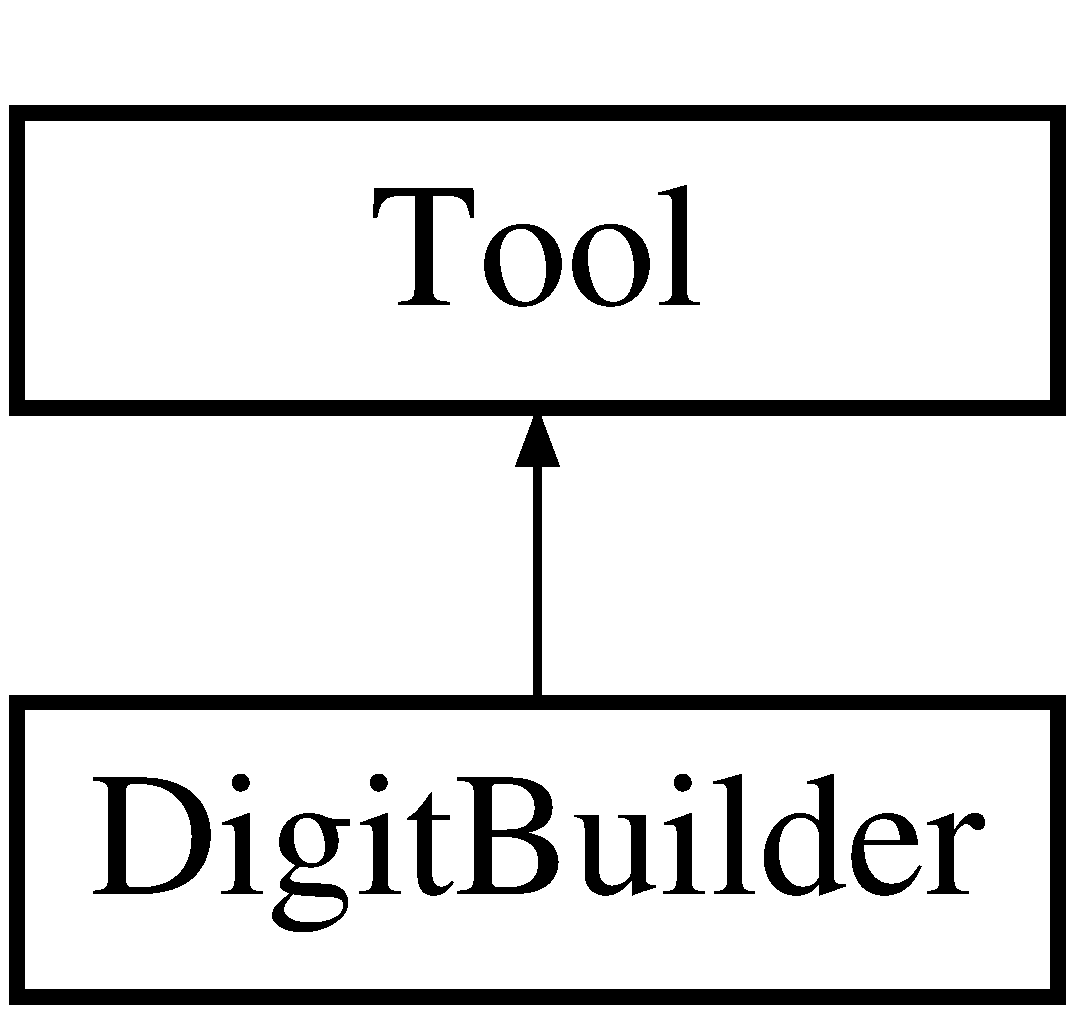
\includegraphics[height=2.000000cm]{classDigitBuilder}
\end{center}
\end{figure}
\subsection*{Public Member Functions}
\begin{DoxyCompactItemize}
\item 
bool \hyperlink{classDigitBuilder_aacb1cb36e5063ba4774381012ac148d6}{Initialise} (std\-::string configfile, \hyperlink{classDataModel}{Data\-Model} \&data)
\item 
bool \hyperlink{classDigitBuilder_a77c2d2d5208563e7a9d8f1a2c8a4777c}{Execute} ()
\item 
\hypertarget{classDigitBuilder_adfbdd3e33b7ac69a7be4bf54fd264066}{bool {\bfseries Finalise} ()}\label{classDigitBuilder_adfbdd3e33b7ac69a7be4bf54fd264066}

\end{DoxyCompactItemize}
\subsection*{Static Public Member Functions}
\begin{DoxyCompactItemize}
\item 
\hypertarget{classDigitBuilder_a3bffe9fa6444a64595122c859d00513d}{static \hyperlink{classDigitBuilder}{Digit\-Builder} $\ast$ {\bfseries Instance} ()}\label{classDigitBuilder_a3bffe9fa6444a64595122c859d00513d}

\end{DoxyCompactItemize}


\subsection{Detailed Description}
This tool reads the raw data from the file and creates a \hyperlink{classDigitBuilder}{Digit\-Builder} object Jingbo Wang \href{mailto:jiowang@ucdavis.edu}{\tt jiowang@ucdavis.\-edu} 

\subsection{Member Function Documentation}
\hypertarget{classDigitBuilder_a77c2d2d5208563e7a9d8f1a2c8a4777c}{\index{Digit\-Builder@{Digit\-Builder}!Execute@{Execute}}
\index{Execute@{Execute}!DigitBuilder@{Digit\-Builder}}
\subsubsection[{Execute}]{\setlength{\rightskip}{0pt plus 5cm}bool Digit\-Builder\-::\-Execute (
\begin{DoxyParamCaption}
{}
\end{DoxyParamCaption}
)}}\label{classDigitBuilder_a77c2d2d5208563e7a9d8f1a2c8a4777c}
Reset everything

see if \char`\"{}\-Reco\-Event\char`\"{} exists. If not, make it

Retrieve necessary info from A\-N\-N\-I\-E\-Event

Build \hyperlink{classRecoDigit}{Reco\-Digit}

\hyperlink{classHit}{Hit} info. to Reco\-Event \hypertarget{classDigitBuilder_aacb1cb36e5063ba4774381012ac148d6}{\index{Digit\-Builder@{Digit\-Builder}!Initialise@{Initialise}}
\index{Initialise@{Initialise}!DigitBuilder@{Digit\-Builder}}
\subsubsection[{Initialise}]{\setlength{\rightskip}{0pt plus 5cm}bool Digit\-Builder\-::\-Initialise (
\begin{DoxyParamCaption}
\item[{std\-::string}]{configfile, }
\item[{{\bf Data\-Model} \&}]{data}
\end{DoxyParamCaption}
)}}\label{classDigitBuilder_aacb1cb36e5063ba4774381012ac148d6}
Get the Tool configuration variables

Construct the other objects we'll be setting at event level, 

The documentation for this class was generated from the following files\-:\begin{DoxyCompactItemize}
\item 
User\-Tools/\-Digit\-Builder/Digit\-Builder.\-h\item 
User\-Tools/\-Digit\-Builder/Digit\-Builder.\-cpp\end{DoxyCompactItemize}

\hypertarget{classDigitBuilderDoE}{\section{Digit\-Builder\-Do\-E Class Reference}
\label{classDigitBuilderDoE}\index{Digit\-Builder\-Do\-E@{Digit\-Builder\-Do\-E}}
}
Inheritance diagram for Digit\-Builder\-Do\-E\-:\begin{figure}[H]
\begin{center}
\leavevmode
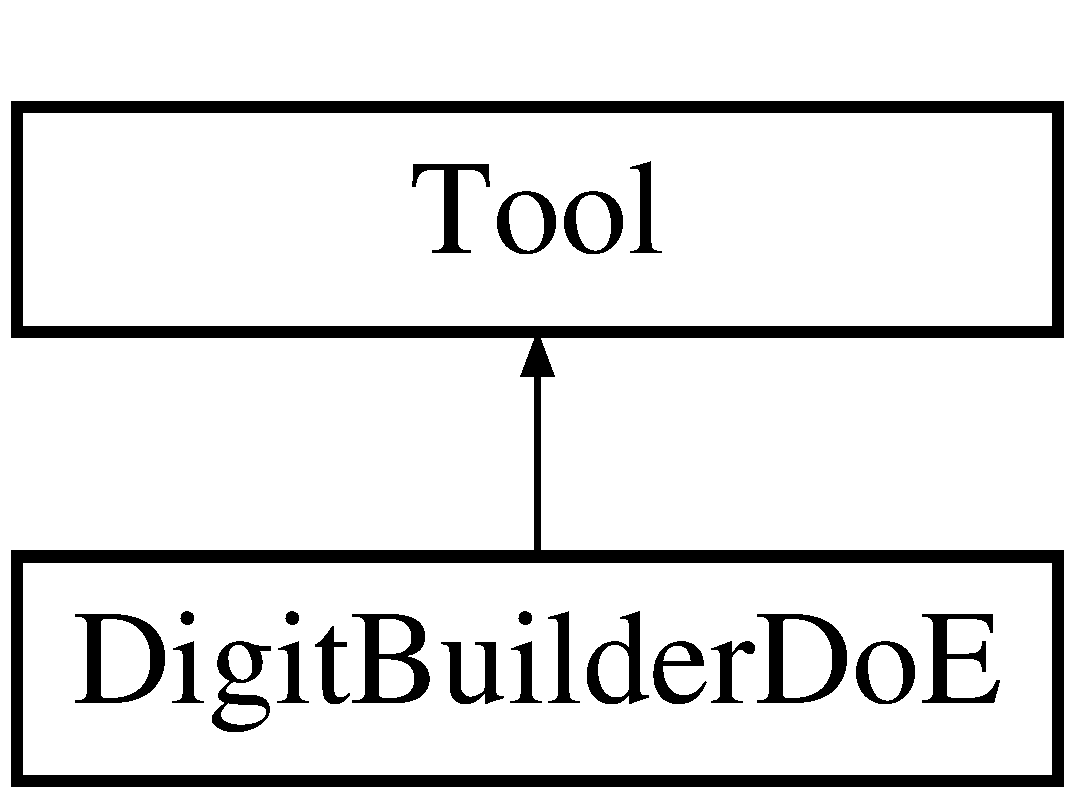
\includegraphics[height=2.000000cm]{classDigitBuilderDoE}
\end{center}
\end{figure}
\subsection*{Public Member Functions}
\begin{DoxyCompactItemize}
\item 
bool \hyperlink{classDigitBuilderDoE_a629487cb173c306f7796d4466049d790}{Initialise} (std\-::string configfile, \hyperlink{classDataModel}{Data\-Model} \&data)
\item 
bool \hyperlink{classDigitBuilderDoE_abbf2b8912d5a5e01c8755ad873e99520}{Execute} ()
\item 
\hypertarget{classDigitBuilderDoE_ad51a7fbe29242cd5f5283a0e1a488798}{bool {\bfseries Finalise} ()}\label{classDigitBuilderDoE_ad51a7fbe29242cd5f5283a0e1a488798}

\end{DoxyCompactItemize}
\subsection*{Static Public Member Functions}
\begin{DoxyCompactItemize}
\item 
\hypertarget{classDigitBuilderDoE_ae6f5d12e2b1c6a3a57097ab946add570}{static \hyperlink{classDigitBuilderDoE}{Digit\-Builder\-Do\-E} $\ast$ {\bfseries Instance} ()}\label{classDigitBuilderDoE_ae6f5d12e2b1c6a3a57097ab946add570}

\end{DoxyCompactItemize}


\subsection{Member Function Documentation}
\hypertarget{classDigitBuilderDoE_abbf2b8912d5a5e01c8755ad873e99520}{\index{Digit\-Builder\-Do\-E@{Digit\-Builder\-Do\-E}!Execute@{Execute}}
\index{Execute@{Execute}!DigitBuilderDoE@{Digit\-Builder\-Do\-E}}
\subsubsection[{Execute}]{\setlength{\rightskip}{0pt plus 5cm}bool Digit\-Builder\-Do\-E\-::\-Execute (
\begin{DoxyParamCaption}
{}
\end{DoxyParamCaption}
)}}\label{classDigitBuilderDoE_abbf2b8912d5a5e01c8755ad873e99520}
see if \char`\"{}\-Reco\-Event\char`\"{} exists

Push recodigits and muon truth info to Reco\-Event \hypertarget{classDigitBuilderDoE_a629487cb173c306f7796d4466049d790}{\index{Digit\-Builder\-Do\-E@{Digit\-Builder\-Do\-E}!Initialise@{Initialise}}
\index{Initialise@{Initialise}!DigitBuilderDoE@{Digit\-Builder\-Do\-E}}
\subsubsection[{Initialise}]{\setlength{\rightskip}{0pt plus 5cm}bool Digit\-Builder\-Do\-E\-::\-Initialise (
\begin{DoxyParamCaption}
\item[{std\-::string}]{configfile, }
\item[{{\bf Data\-Model} \&}]{data}
\end{DoxyParamCaption}
)}}\label{classDigitBuilderDoE_a629487cb173c306f7796d4466049d790}
Construct the other objects we'll be setting at event level, 

The documentation for this class was generated from the following files\-:\begin{DoxyCompactItemize}
\item 
User\-Tools/\-Digit\-Builder\-Do\-E/Digit\-Builder\-Do\-E.\-h\item 
User\-Tools/\-Digit\-Builder\-Do\-E/Digit\-Builder\-Do\-E.\-cpp\end{DoxyCompactItemize}

\hypertarget{classDigitBuilderROOT}{
\section{DigitBuilderROOT Class Reference}
\label{classDigitBuilderROOT}\index{DigitBuilderROOT@{DigitBuilderROOT}}
}
\subsection*{Public Member Functions}
\begin{DoxyCompactItemize}
\item 
\hypertarget{classDigitBuilderROOT_a7ab06541c442a8bc03adc0c7a4b32086}{
bool {\bfseries Initialise} (std::string configfile, \hyperlink{classDataModel}{DataModel} \&data)}
\label{classDigitBuilderROOT_a7ab06541c442a8bc03adc0c7a4b32086}

\item 
\hypertarget{classDigitBuilderROOT_a9529acec5b1a6cf468e57c96bf55453d}{
bool {\bfseries Execute} ()}
\label{classDigitBuilderROOT_a9529acec5b1a6cf468e57c96bf55453d}

\item 
\hypertarget{classDigitBuilderROOT_a1beb47fea60dc16f627a339ee0597e71}{
bool {\bfseries Finalise} ()}
\label{classDigitBuilderROOT_a1beb47fea60dc16f627a339ee0597e71}

\item 
\hypertarget{classDigitBuilderROOT_a894cb087ddb66f65fe966d4155b03256}{
void {\bfseries PushTrueVertex} (bool savetodisk)}
\label{classDigitBuilderROOT_a894cb087ddb66f65fe966d4155b03256}

\item 
void \hyperlink{classDigitBuilderROOT_af623aff0f8d4b58cb4c7182da49b76b7}{PushRecoDigits} (bool savetodisk)
\item 
void \hyperlink{classDigitBuilderROOT_a7edde994bef160f405d740b5e9b01176}{PushTrueWaterTrackLength} (double WaterT)
\item 
void \hyperlink{classDigitBuilderROOT_adca0d96fa944b38e44e2ebb8a619f77b}{PushTrueMRDTrackLength} (double MRDT)
\item 
\hypertarget{classDigitBuilderROOT_a01cd5fb15e6ebe304ba751652de2b37b}{
void {\bfseries Reset} ()}
\label{classDigitBuilderROOT_a01cd5fb15e6ebe304ba751652de2b37b}

\end{DoxyCompactItemize}


\subsection{Member Function Documentation}
\hypertarget{classDigitBuilderROOT_af623aff0f8d4b58cb4c7182da49b76b7}{
\index{DigitBuilderROOT@{DigitBuilderROOT}!PushRecoDigits@{PushRecoDigits}}
\index{PushRecoDigits@{PushRecoDigits}!DigitBuilderROOT@{DigitBuilderROOT}}
\subsubsection[{PushRecoDigits}]{\setlength{\rightskip}{0pt plus 5cm}void DigitBuilderROOT::PushRecoDigits (bool {\em savetodisk})}}
\label{classDigitBuilderROOT_af623aff0f8d4b58cb4c7182da49b76b7}


$>$ Add digits to RecoEvent \hypertarget{classDigitBuilderROOT_adca0d96fa944b38e44e2ebb8a619f77b}{
\index{DigitBuilderROOT@{DigitBuilderROOT}!PushTrueMRDTrackLength@{PushTrueMRDTrackLength}}
\index{PushTrueMRDTrackLength@{PushTrueMRDTrackLength}!DigitBuilderROOT@{DigitBuilderROOT}}
\subsubsection[{PushTrueMRDTrackLength}]{\setlength{\rightskip}{0pt plus 5cm}void DigitBuilderROOT::PushTrueMRDTrackLength (double {\em MRDT})}}
\label{classDigitBuilderROOT_adca0d96fa944b38e44e2ebb8a619f77b}


$>$ Add digits to RecoEvent \hypertarget{classDigitBuilderROOT_a7edde994bef160f405d740b5e9b01176}{
\index{DigitBuilderROOT@{DigitBuilderROOT}!PushTrueWaterTrackLength@{PushTrueWaterTrackLength}}
\index{PushTrueWaterTrackLength@{PushTrueWaterTrackLength}!DigitBuilderROOT@{DigitBuilderROOT}}
\subsubsection[{PushTrueWaterTrackLength}]{\setlength{\rightskip}{0pt plus 5cm}void DigitBuilderROOT::PushTrueWaterTrackLength (double {\em WaterT})}}
\label{classDigitBuilderROOT_a7edde994bef160f405d740b5e9b01176}


$>$ Add digits to RecoEvent 

The documentation for this class was generated from the following files:\begin{DoxyCompactItemize}
\item 
UserTools/DigitBuilderROOT/DigitBuilderROOT.h\item 
UserTools/DigitBuilderROOT/DigitBuilderROOT.cpp\end{DoxyCompactItemize}

\hypertarget{classDirection}{
\section{Direction Class Reference}
\label{classDirection}\index{Direction@{Direction}}
}
Inheritance diagram for Direction::\begin{figure}[H]
\begin{center}
\leavevmode
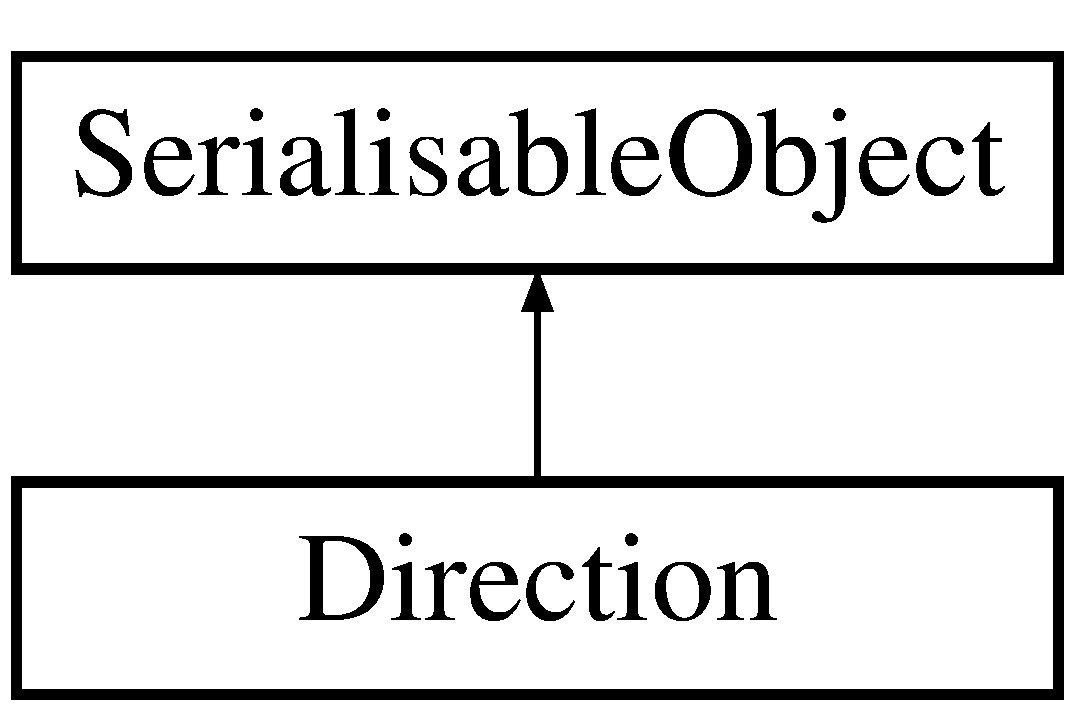
\includegraphics[height=2cm]{classDirection}
\end{center}
\end{figure}
\subsection*{Public Member Functions}
\begin{DoxyCompactItemize}
\item 
\hypertarget{classDirection_a6ab97d45f5cba3aa5e571f0c0e8dd5be}{
{\bfseries Direction} (double xin, double yin, double zin)}
\label{classDirection_a6ab97d45f5cba3aa5e571f0c0e8dd5be}

\item 
\hypertarget{classDirection_ae577ffea4af24ebc490093c55adbbdba}{
{\bfseries Direction} (double phiin, double thetain)}
\label{classDirection_ae577ffea4af24ebc490093c55adbbdba}

\item 
\hypertarget{classDirection_a16e35cd86702666a7f2a9de1962b99d3}{
double {\bfseries X} () const }
\label{classDirection_a16e35cd86702666a7f2a9de1962b99d3}

\item 
\hypertarget{classDirection_a87038a7a2381c3bfa062d1016ece1b0a}{
double {\bfseries Y} () const }
\label{classDirection_a87038a7a2381c3bfa062d1016ece1b0a}

\item 
\hypertarget{classDirection_a7e8275fe3078f9fb2c4f17cafd219dca}{
double {\bfseries Z} () const }
\label{classDirection_a7e8275fe3078f9fb2c4f17cafd219dca}

\item 
\hypertarget{classDirection_ae60296b4e458a378de7fac5e194d128a}{
double {\bfseries GetPhi} () const }
\label{classDirection_ae60296b4e458a378de7fac5e194d128a}

\item 
\hypertarget{classDirection_ab10dd98d45f913882643a8ec3a0063a1}{
double {\bfseries GetPhiDeg} () const }
\label{classDirection_ab10dd98d45f913882643a8ec3a0063a1}

\item 
\hypertarget{classDirection_aedb9b4a05e136edbb8d9ff19b84a5698}{
double {\bfseries GetTheta} () const }
\label{classDirection_aedb9b4a05e136edbb8d9ff19b84a5698}

\item 
\hypertarget{classDirection_a3ed1c31e69e15d4b6a50aeb5bbf48049}{
double {\bfseries GetThetaDeg} () const }
\label{classDirection_a3ed1c31e69e15d4b6a50aeb5bbf48049}

\item 
\hypertarget{classDirection_a384688a73b4fea94e29f76401c329588}{
void {\bfseries SetX} (double xx)}
\label{classDirection_a384688a73b4fea94e29f76401c329588}

\item 
\hypertarget{classDirection_a879833b6fdb717fa5eee797e9fa37110}{
void {\bfseries SetY} (double yy)}
\label{classDirection_a879833b6fdb717fa5eee797e9fa37110}

\item 
\hypertarget{classDirection_af79a87b020ea1122d7754f8c382e5973}{
void {\bfseries SetZ} (double zz)}
\label{classDirection_af79a87b020ea1122d7754f8c382e5973}

\item 
\hypertarget{classDirection_acb7c66942c436968aa207945362afdc0}{
void {\bfseries SetPhi} (double ph)}
\label{classDirection_acb7c66942c436968aa207945362afdc0}

\item 
\hypertarget{classDirection_a1d14bbfe02ca398b2cd6ae175cd05a8a}{
void {\bfseries SetPhiDeg} (double phd)}
\label{classDirection_a1d14bbfe02ca398b2cd6ae175cd05a8a}

\item 
\hypertarget{classDirection_ac14dae5fc8c04039b68f5c4afa1444de}{
void {\bfseries SetTheta} (double th)}
\label{classDirection_ac14dae5fc8c04039b68f5c4afa1444de}

\item 
\hypertarget{classDirection_aed59dbad937a7d05bd7bb90344869e32}{
void {\bfseries SetThetaDeg} (double thd)}
\label{classDirection_aed59dbad937a7d05bd7bb90344869e32}

\item 
\hypertarget{classDirection_aa0dc919856fbf935470d8e34d042bc9a}{
bool {\bfseries Print} ()}
\label{classDirection_aa0dc919856fbf935470d8e34d042bc9a}

\end{DoxyCompactItemize}
\subsection*{Friends}
\begin{DoxyCompactItemize}
\item 
\hypertarget{classDirection_ac98d07dd8f7b70e16ccb9a01abf56b9c}{
class {\bfseries boost::serialization::access}}
\label{classDirection_ac98d07dd8f7b70e16ccb9a01abf56b9c}

\end{DoxyCompactItemize}


The documentation for this class was generated from the following file:\begin{DoxyCompactItemize}
\item 
DataModel/Direction.h\end{DoxyCompactItemize}

\hypertarget{classDummyTool}{\section{Dummy\-Tool Class Reference}
\label{classDummyTool}\index{Dummy\-Tool@{Dummy\-Tool}}
}


{\ttfamily \#include $<$Dummy\-Tool.\-h$>$}

Inheritance diagram for Dummy\-Tool\-:\begin{figure}[H]
\begin{center}
\leavevmode
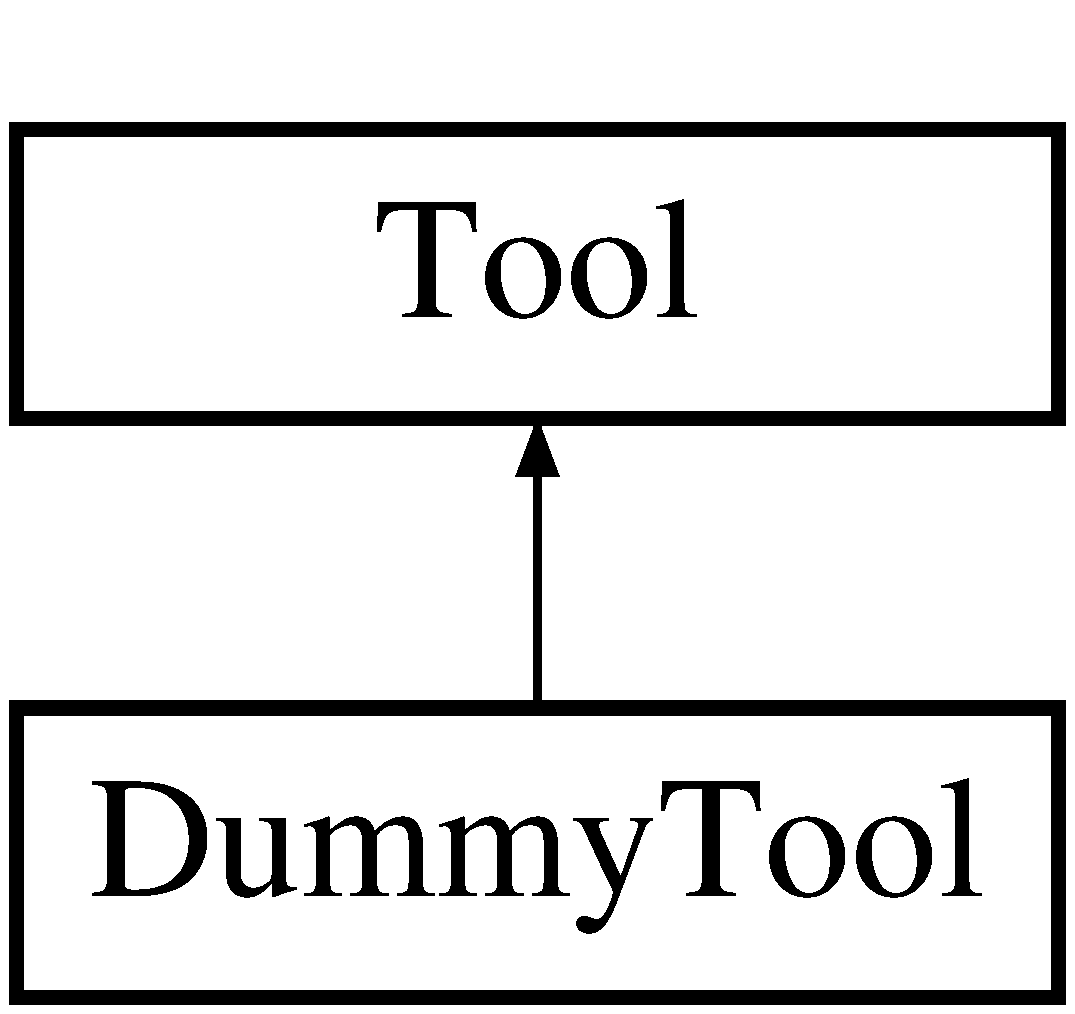
\includegraphics[height=2.000000cm]{classDummyTool}
\end{center}
\end{figure}
\subsection*{Public Member Functions}
\begin{DoxyCompactItemize}
\item 
\hypertarget{classDummyTool_a33914471b4de346168aa92b5febb6f9c}{\hyperlink{classDummyTool_a33914471b4de346168aa92b5febb6f9c}{Dummy\-Tool} ()}\label{classDummyTool_a33914471b4de346168aa92b5febb6f9c}

\begin{DoxyCompactList}\small\item\em Constructor. \end{DoxyCompactList}\item 
\hypertarget{classDummyTool_a0d9cd781681a06ee3cf0cd1e7bb770a8}{bool \hyperlink{classDummyTool_a0d9cd781681a06ee3cf0cd1e7bb770a8}{Initialise} (std\-::string configfile, \hyperlink{classDataModel}{Data\-Model} \&data)}\label{classDummyTool_a0d9cd781681a06ee3cf0cd1e7bb770a8}

\begin{DoxyCompactList}\small\item\em Assigns verbosity from config file and creates a log message. \end{DoxyCompactList}\item 
\hypertarget{classDummyTool_ac107b31f1785c1cc803e0e65be548047}{bool \hyperlink{classDummyTool_ac107b31f1785c1cc803e0e65be548047}{Execute} ()}\label{classDummyTool_ac107b31f1785c1cc803e0e65be548047}

\begin{DoxyCompactList}\small\item\em Creates a log message. \end{DoxyCompactList}\item 
\hypertarget{classDummyTool_aacb5d0b9906a27c2b4bba4aae9bc093a}{bool \hyperlink{classDummyTool_aacb5d0b9906a27c2b4bba4aae9bc093a}{Finalise} ()}\label{classDummyTool_aacb5d0b9906a27c2b4bba4aae9bc093a}

\begin{DoxyCompactList}\small\item\em Does nothing. \end{DoxyCompactList}\end{DoxyCompactItemize}


\subsection{Detailed Description}
This is a simple dummy Tool designed to show operation of a Tool. It also provides a default Tool for the Default Tool\-Chain.

\begin{DoxyParagraph}{Author\-:}
B.\-Richards 
\end{DoxyParagraph}
\begin{DoxyParagraph}{Date\-:}
2019/05/28 10\-:44\-:00 
\end{DoxyParagraph}
Contact\-: \href{mailto:b.richards@qmul.ac.uk}{\tt b.\-richards@qmul.\-ac.\-uk} 

The documentation for this class was generated from the following files\-:\begin{DoxyCompactItemize}
\item 
User\-Tools/\-Examples/Dummy\-Tool.\-h\item 
User\-Tools/\-Examples/Dummy\-Tool.\-cpp\end{DoxyCompactItemize}

\hypertarget{classEventDisplay}{\section{Event\-Display Class Reference}
\label{classEventDisplay}\index{Event\-Display@{Event\-Display}}
}
Inheritance diagram for Event\-Display\-:\begin{figure}[H]
\begin{center}
\leavevmode
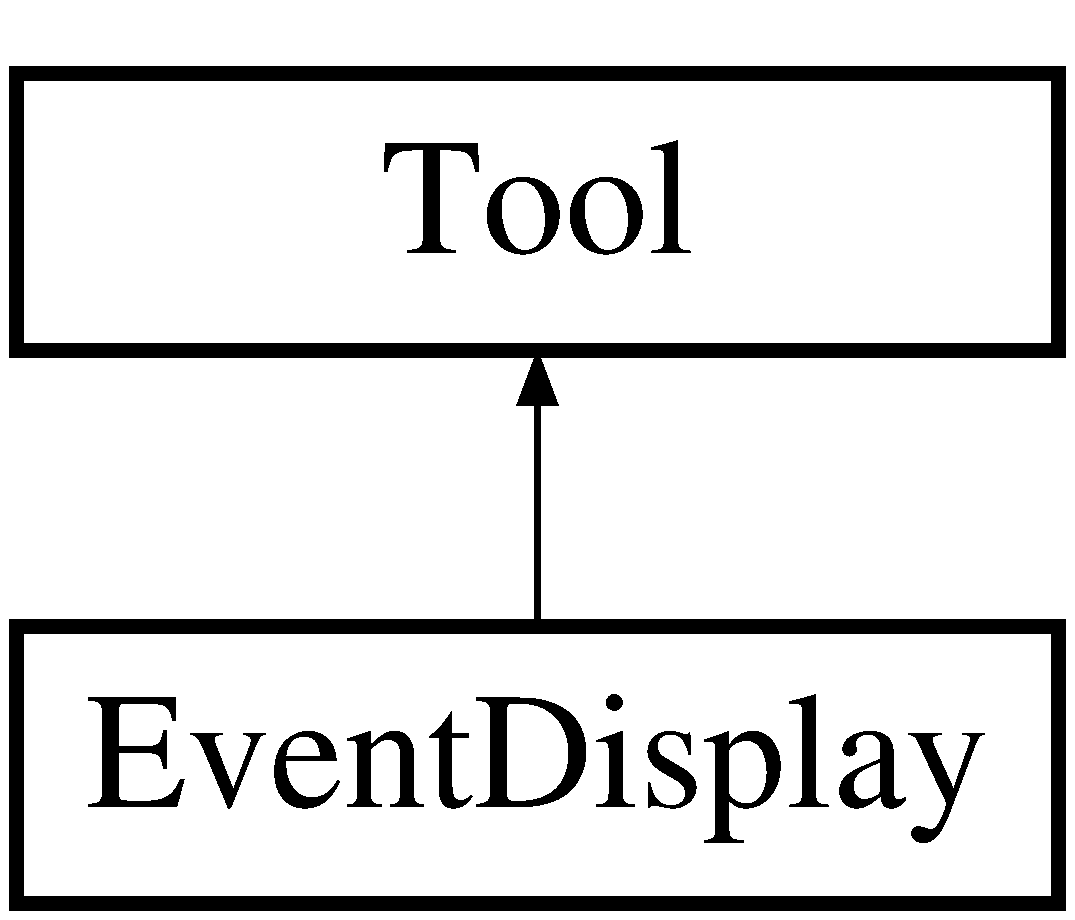
\includegraphics[height=2.000000cm]{classEventDisplay}
\end{center}
\end{figure}
\subsection*{Public Member Functions}
\begin{DoxyCompactItemize}
\item 
\hypertarget{classEventDisplay_afc7edf8f24c74b37c29355745b3cc4ad}{bool {\bfseries Initialise} (std\-::string configfile, \hyperlink{classDataModel}{Data\-Model} \&data)}\label{classEventDisplay_afc7edf8f24c74b37c29355745b3cc4ad}

\item 
\hypertarget{classEventDisplay_a3468ff690ccecd91c2b7ee84021d5e4b}{bool {\bfseries Execute} ()}\label{classEventDisplay_a3468ff690ccecd91c2b7ee84021d5e4b}

\item 
\hypertarget{classEventDisplay_a0fdfbdba7f66663ca61a2015c3f87a27}{bool {\bfseries Finalise} ()}\label{classEventDisplay_a0fdfbdba7f66663ca61a2015c3f87a27}

\item 
\hypertarget{classEventDisplay_a0badd7d4c163fd33246ef2fb5f3f5b11}{void {\bfseries make\-\_\-gui} ()}\label{classEventDisplay_a0badd7d4c163fd33246ef2fb5f3f5b11}

\item 
\hypertarget{classEventDisplay_acdb0b7db7007c50303e29321e8b178df}{void {\bfseries draw\-\_\-event} ()}\label{classEventDisplay_acdb0b7db7007c50303e29321e8b178df}

\item 
\hypertarget{classEventDisplay_a45064b5628a451ee019e2dc47fb80268}{void {\bfseries draw\-\_\-event\-\_\-box} ()}\label{classEventDisplay_a45064b5628a451ee019e2dc47fb80268}

\item 
\hypertarget{classEventDisplay_a7ffd0d9f6b41b5713655e11e8d79840c}{void {\bfseries draw\-\_\-pmt\-\_\-legend} ()}\label{classEventDisplay_a7ffd0d9f6b41b5713655e11e8d79840c}

\item 
\hypertarget{classEventDisplay_a1405448b0dafae76a5ff4bcbb1bc2fa4}{void {\bfseries draw\-\_\-lappd\-\_\-legend} ()}\label{classEventDisplay_a1405448b0dafae76a5ff4bcbb1bc2fa4}

\item 
\hypertarget{classEventDisplay_a69683e114fa3e1702ba154789672f492}{void {\bfseries draw\-\_\-event\-\_\-\-P\-M\-Ts} ()}\label{classEventDisplay_a69683e114fa3e1702ba154789672f492}

\item 
\hypertarget{classEventDisplay_ae0d1b0fb901484e92518ec76061c5c9c}{void {\bfseries draw\-\_\-event\-\_\-\-L\-A\-P\-P\-Ds} ()}\label{classEventDisplay_ae0d1b0fb901484e92518ec76061c5c9c}

\item 
\hypertarget{classEventDisplay_a8c3315cc4f055772b275e7a5c9593526}{void {\bfseries draw\-\_\-event\-\_\-\-M\-R\-D} ()}\label{classEventDisplay_a8c3315cc4f055772b275e7a5c9593526}

\item 
\hypertarget{classEventDisplay_a13ff76de80459d2b68e24dbd0b24416e}{void {\bfseries draw\-\_\-true\-\_\-vertex} ()}\label{classEventDisplay_a13ff76de80459d2b68e24dbd0b24416e}

\item 
\hypertarget{classEventDisplay_ad9e11e4c29bf6cd9c616e8a88c9450a5}{void {\bfseries draw\-\_\-true\-\_\-ring} ()}\label{classEventDisplay_ad9e11e4c29bf6cd9c616e8a88c9450a5}

\item 
\hypertarget{classEventDisplay_a0c142aae987bce6741becd4254993e4b}{void {\bfseries delete\-\_\-canvas\-\_\-contents} ()}\label{classEventDisplay_a0c142aae987bce6741becd4254993e4b}

\item 
\hypertarget{classEventDisplay_a8e03ad3c8e618e6781a8e085d4577083}{void {\bfseries draw\-\_\-schematic\-\_\-detector} ()}\label{classEventDisplay_a8e03ad3c8e618e6781a8e085d4577083}

\item 
\hypertarget{classEventDisplay_a8e0374381693a843b58d33ac4a3debd9}{void {\bfseries set\-\_\-color\-\_\-palette} ()}\label{classEventDisplay_a8e0374381693a843b58d33ac4a3debd9}

\item 
\hypertarget{classEventDisplay_a3e7298c6aab4ea268f51a6c805ccdc9a}{void {\bfseries translate\-\_\-xy} (double vtx\-X, double vtx\-Y, double vtx\-Z, double \&x\-Wall, double \&y\-Wall, int \&status\-\_\-hit, double \&phi\-\_\-calc)}\label{classEventDisplay_a3e7298c6aab4ea268f51a6c805ccdc9a}

\item 
\hypertarget{classEventDisplay_a0a3b0b46289031922181d43a7db56271}{void {\bfseries find\-\_\-projected\-\_\-xyz} (double vtx\-X, double vtx\-Y, double vtx\-Z, double dir\-X, double dir\-Y, double dir\-Z, double \&projected\-\_\-x, double \&projected\-\_\-y, double \&projected\-\_\-z)}\label{classEventDisplay_a0a3b0b46289031922181d43a7db56271}

\end{DoxyCompactItemize}


The documentation for this class was generated from the following files\-:\begin{DoxyCompactItemize}
\item 
User\-Tools/\-Event\-Display/Event\-Display.\-h\item 
User\-Tools/\-Event\-Display/Event\-Display.\-cpp\end{DoxyCompactItemize}

\hypertarget{classEventSelector}{
\section{EventSelector Class Reference}
\label{classEventSelector}\index{EventSelector@{EventSelector}}
}
\subsection*{Public Types}
\begin{DoxyCompactItemize}
\item 
enum {\bfseries EventFlags} \{ \par
{\bfseries kFlagNone} =  0x00, 
{\bfseries kFlagMCFV} =  0x01, 
{\bfseries kFlagMCPMTVol} =  0x02, 
{\bfseries kFlagMCMRD} =  0x04, 
\par
{\bfseries kFlagMCPiK} =  0x08, 
{\bfseries kFlagRecoMRD} =  0x10, 
{\bfseries kFlagPromptTrig} =  0x20, 
{\bfseries kFlagNHit} =  0x40, 
\par
{\bfseries kFlagRecoFV} =  0x80, 
{\bfseries kFlagRecoPMTVol} =  0x100
 \}
\item 
\hypertarget{classEventSelector_ab9f5d192d2badda9754e2e91f430a012}{
typedef enum EventSelector::EventFlags {\bfseries EventFlags\_\-t}}
\label{classEventSelector_ab9f5d192d2badda9754e2e91f430a012}

\end{DoxyCompactItemize}
\subsection*{Public Member Functions}
\begin{DoxyCompactItemize}
\item 
bool \hyperlink{classEventSelector_a839f44332021b0345d0277f68ae612a8}{Initialise} (std::string configfile, \hyperlink{classDataModel}{DataModel} \&data)
\item 
bool \hyperlink{classEventSelector_a0edbb6c1b1a8c3fcd9453d3dd5796005}{Execute} ()
\item 
\hypertarget{classEventSelector_a73c813845d7cfce13f160e94b44b56c1}{
bool {\bfseries Finalise} ()}
\label{classEventSelector_a73c813845d7cfce13f160e94b44b56c1}

\end{DoxyCompactItemize}


\subsection{Member Function Documentation}
\hypertarget{classEventSelector_a0edbb6c1b1a8c3fcd9453d3dd5796005}{
\index{EventSelector@{EventSelector}!Execute@{Execute}}
\index{Execute@{Execute}!EventSelector@{EventSelector}}
\subsubsection[{Execute}]{\setlength{\rightskip}{0pt plus 5cm}bool EventSelector::Execute ()}}
\label{classEventSelector_a0edbb6c1b1a8c3fcd9453d3dd5796005}


$>$ Get digits from \char`\"{}RecoEvent\char`\"{}

$>$ Get reconstructed vertex \hypertarget{classEventSelector_a839f44332021b0345d0277f68ae612a8}{
\index{EventSelector@{EventSelector}!Initialise@{Initialise}}
\index{Initialise@{Initialise}!EventSelector@{EventSelector}}
\subsubsection[{Initialise}]{\setlength{\rightskip}{0pt plus 5cm}bool EventSelector::Initialise (std::string {\em configfile}, \/  {\bf DataModel} \& {\em data})}}
\label{classEventSelector_a839f44332021b0345d0277f68ae612a8}


Construct the other objects we'll be needing at event level, 

The documentation for this class was generated from the following files:\begin{DoxyCompactItemize}
\item 
UserTools/EventSelector/EventSelector.h\item 
UserTools/EventSelector/EventSelector.cpp\end{DoxyCompactItemize}

\hypertarget{classEventSelectorDoE}{\section{Event\-Selector\-Do\-E Class Reference}
\label{classEventSelectorDoE}\index{Event\-Selector\-Do\-E@{Event\-Selector\-Do\-E}}
}
Inheritance diagram for Event\-Selector\-Do\-E\-:\begin{figure}[H]
\begin{center}
\leavevmode
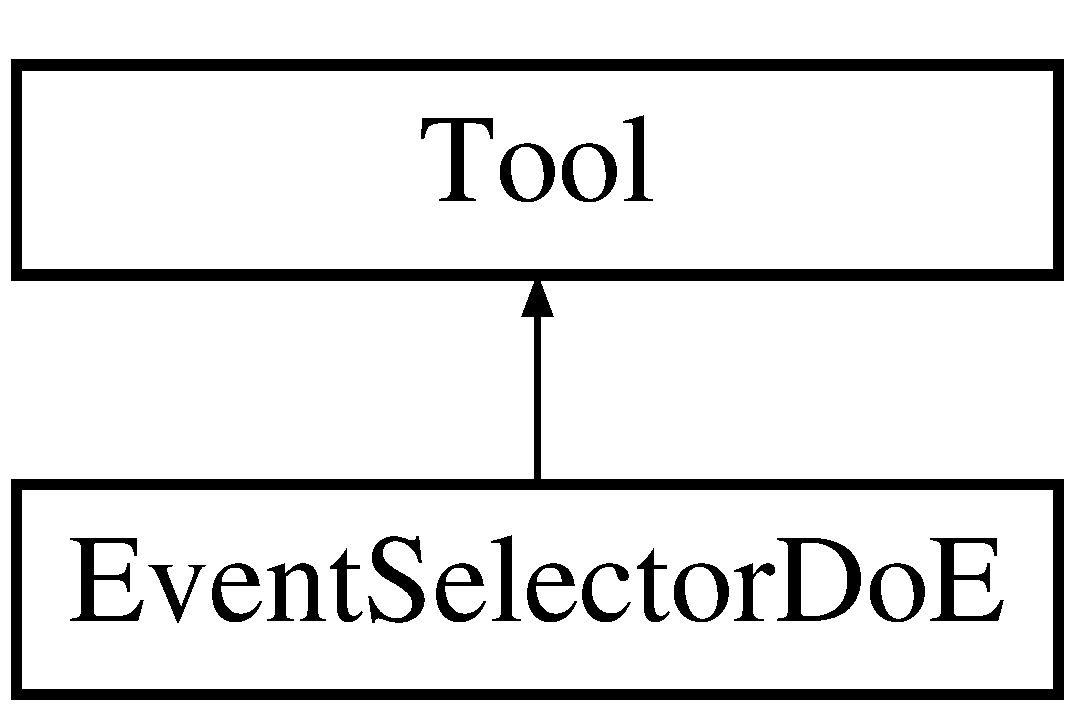
\includegraphics[height=2.000000cm]{classEventSelectorDoE}
\end{center}
\end{figure}
\subsection*{Public Member Functions}
\begin{DoxyCompactItemize}
\item 
bool \hyperlink{classEventSelectorDoE_a9eef7438e552c60c6c11b3977d2f9210}{Initialise} (std\-::string configfile, \hyperlink{classDataModel}{Data\-Model} \&data)
\item 
\hypertarget{classEventSelectorDoE_afa76e234da6aef6333dca180b0a0e281}{bool {\bfseries Execute} ()}\label{classEventSelectorDoE_afa76e234da6aef6333dca180b0a0e281}

\item 
\hypertarget{classEventSelectorDoE_a2463b7db3877856bd0ce12b3e00dc8f9}{bool {\bfseries Finalise} ()}\label{classEventSelectorDoE_a2463b7db3877856bd0ce12b3e00dc8f9}

\end{DoxyCompactItemize}


\subsection{Member Function Documentation}
\hypertarget{classEventSelectorDoE_a9eef7438e552c60c6c11b3977d2f9210}{\index{Event\-Selector\-Do\-E@{Event\-Selector\-Do\-E}!Initialise@{Initialise}}
\index{Initialise@{Initialise}!EventSelectorDoE@{Event\-Selector\-Do\-E}}
\subsubsection[{Initialise}]{\setlength{\rightskip}{0pt plus 5cm}bool Event\-Selector\-Do\-E\-::\-Initialise (
\begin{DoxyParamCaption}
\item[{std\-::string}]{configfile, }
\item[{{\bf Data\-Model} \&}]{data}
\end{DoxyParamCaption}
)}}\label{classEventSelectorDoE_a9eef7438e552c60c6c11b3977d2f9210}
Construct the other objects we'll be setting at event level, 

The documentation for this class was generated from the following files\-:\begin{DoxyCompactItemize}
\item 
User\-Tools/\-Event\-Selector\-Do\-E/Event\-Selector\-Do\-E.\-h\item 
User\-Tools/\-Event\-Selector\-Do\-E/Event\-Selector\-Do\-E.\-cpp\end{DoxyCompactItemize}

\hypertarget{classExampleGenerateData}{
\section{ExampleGenerateData Class Reference}
\label{classExampleGenerateData}\index{ExampleGenerateData@{ExampleGenerateData}}
}
\subsection*{Public Member Functions}
\begin{DoxyCompactItemize}
\item 
\hypertarget{classExampleGenerateData_a34ef11ea9d2fe02c76c13227855538c7}{
bool {\bfseries Initialise} (std::string configfile, \hyperlink{classDataModel}{DataModel} \&data)}
\label{classExampleGenerateData_a34ef11ea9d2fe02c76c13227855538c7}

\item 
\hypertarget{classExampleGenerateData_a8ad50d91b736d2f11f48db3179ac7019}{
bool {\bfseries Execute} ()}
\label{classExampleGenerateData_a8ad50d91b736d2f11f48db3179ac7019}

\item 
\hypertarget{classExampleGenerateData_a7d27959b6641603076134866022f5ee9}{
bool {\bfseries Finalise} ()}
\label{classExampleGenerateData_a7d27959b6641603076134866022f5ee9}

\end{DoxyCompactItemize}


The documentation for this class was generated from the following files:\begin{DoxyCompactItemize}
\item 
UserTools/Examples/ExampleGenerateData.h\item 
UserTools/Examples/ExampleGenerateData.cpp\end{DoxyCompactItemize}

\hypertarget{classExampleLoadRoot}{\section{Example\-Load\-Root Class Reference}
\label{classExampleLoadRoot}\index{Example\-Load\-Root@{Example\-Load\-Root}}
}
Inheritance diagram for Example\-Load\-Root\-:\begin{figure}[H]
\begin{center}
\leavevmode
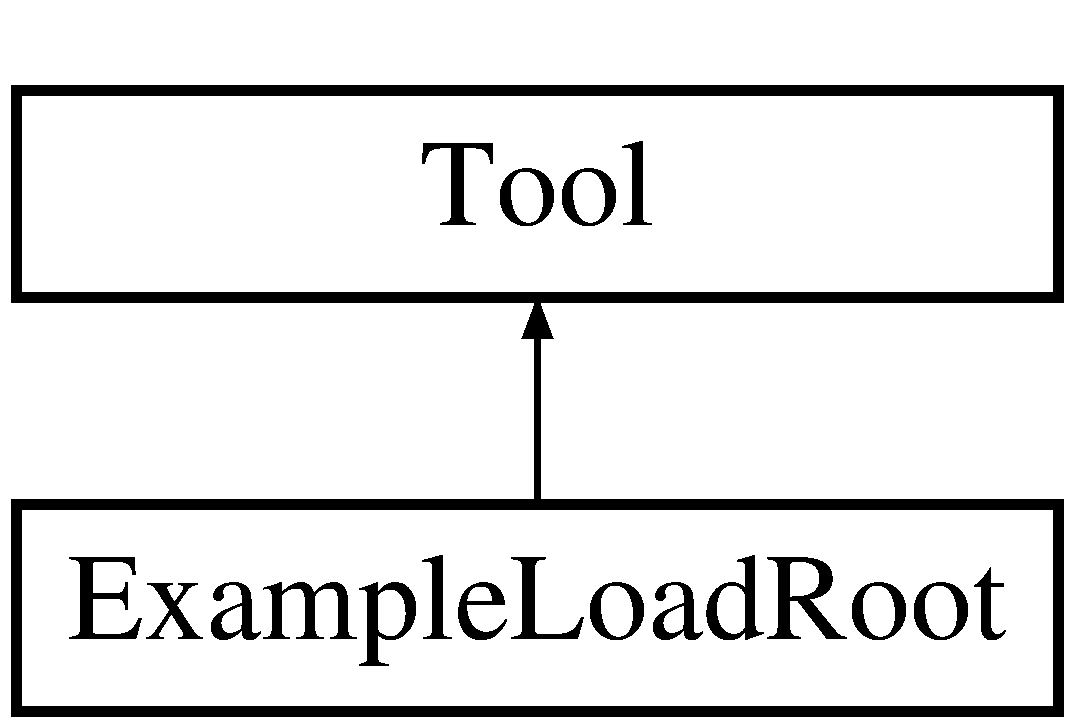
\includegraphics[height=2.000000cm]{classExampleLoadRoot}
\end{center}
\end{figure}
\subsection*{Public Member Functions}
\begin{DoxyCompactItemize}
\item 
\hypertarget{classExampleLoadRoot_a35f783852deea4191cf82812ccbd743c}{bool {\bfseries Initialise} (std\-::string configfile, \hyperlink{classDataModel}{Data\-Model} \&data)}\label{classExampleLoadRoot_a35f783852deea4191cf82812ccbd743c}

\item 
bool \hyperlink{classExampleLoadRoot_a463f4b53011e5fa862a3d39058305b83}{Execute} ()
\item 
\hypertarget{classExampleLoadRoot_aa919eb5fb4d16a7cf632b80a592970f2}{bool {\bfseries Finalise} ()}\label{classExampleLoadRoot_aa919eb5fb4d16a7cf632b80a592970f2}

\end{DoxyCompactItemize}


\subsection{Member Function Documentation}
\hypertarget{classExampleLoadRoot_a463f4b53011e5fa862a3d39058305b83}{\index{Example\-Load\-Root@{Example\-Load\-Root}!Execute@{Execute}}
\index{Execute@{Execute}!ExampleLoadRoot@{Example\-Load\-Root}}
\subsubsection[{Execute}]{\setlength{\rightskip}{0pt plus 5cm}bool Example\-Load\-Root\-::\-Execute (
\begin{DoxyParamCaption}
{}
\end{DoxyParamCaption}
)}}\label{classExampleLoadRoot_a463f4b53011e5fa862a3d39058305b83}
saving to store for the sake of printing 

The documentation for this class was generated from the following files\-:\begin{DoxyCompactItemize}
\item 
User\-Tools/\-Examples/Example\-Load\-Root.\-h\item 
User\-Tools/\-Examples/Example\-Load\-Root.\-cpp\end{DoxyCompactItemize}

\hypertarget{classExampleloadStore}{\section{Exampleload\-Store Class Reference}
\label{classExampleloadStore}\index{Exampleload\-Store@{Exampleload\-Store}}
}
Inheritance diagram for Exampleload\-Store\-:\begin{figure}[H]
\begin{center}
\leavevmode
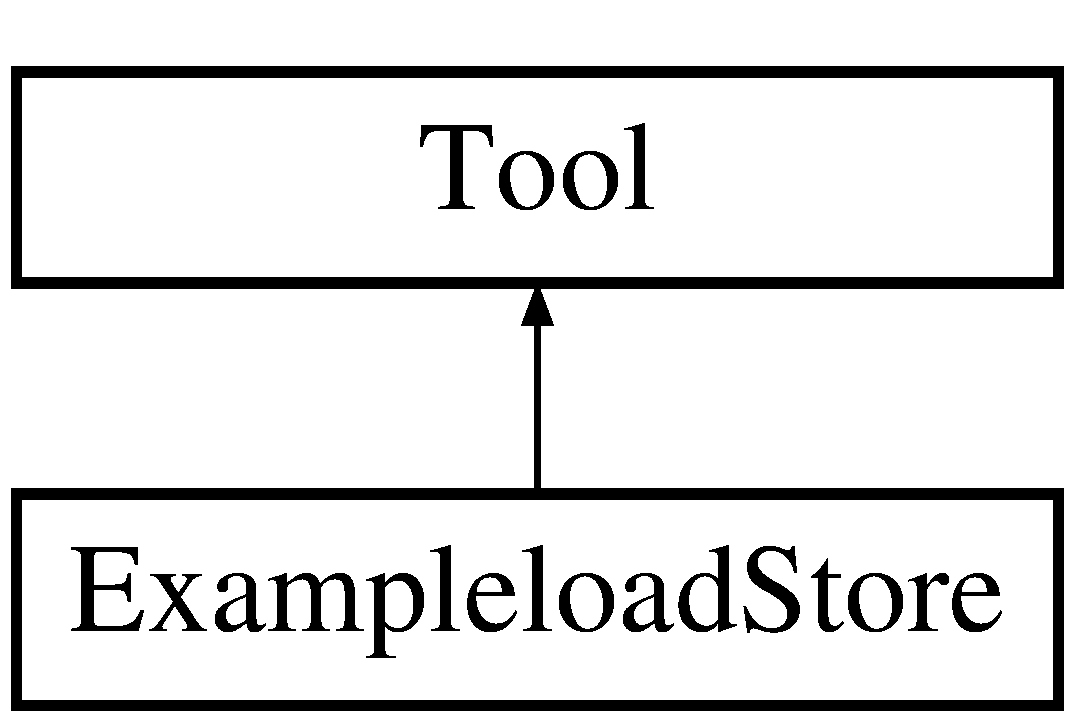
\includegraphics[height=2.000000cm]{classExampleloadStore}
\end{center}
\end{figure}
\subsection*{Public Member Functions}
\begin{DoxyCompactItemize}
\item 
\hypertarget{classExampleloadStore_aa36ea82e625367750cf90f47b68b4868}{bool {\bfseries Initialise} (std\-::string configfile, \hyperlink{classDataModel}{Data\-Model} \&data)}\label{classExampleloadStore_aa36ea82e625367750cf90f47b68b4868}

\item 
\hypertarget{classExampleloadStore_abb8ad989ae4890d9058989e9f4c1c5a7}{bool {\bfseries Execute} ()}\label{classExampleloadStore_abb8ad989ae4890d9058989e9f4c1c5a7}

\item 
\hypertarget{classExampleloadStore_a0170aae0ee1e46ea8e6132fb4874bb8d}{bool {\bfseries Finalise} ()}\label{classExampleloadStore_a0170aae0ee1e46ea8e6132fb4874bb8d}

\end{DoxyCompactItemize}


The documentation for this class was generated from the following files\-:\begin{DoxyCompactItemize}
\item 
User\-Tools/\-Examples/Exampleload\-Store.\-h\item 
User\-Tools/\-Examples/Exampleload\-Store.\-cpp\end{DoxyCompactItemize}

\hypertarget{classExampleOverTool}{\section{Example\-Over\-Tool Class Reference}
\label{classExampleOverTool}\index{Example\-Over\-Tool@{Example\-Over\-Tool}}
}
Inheritance diagram for Example\-Over\-Tool\-:\begin{figure}[H]
\begin{center}
\leavevmode
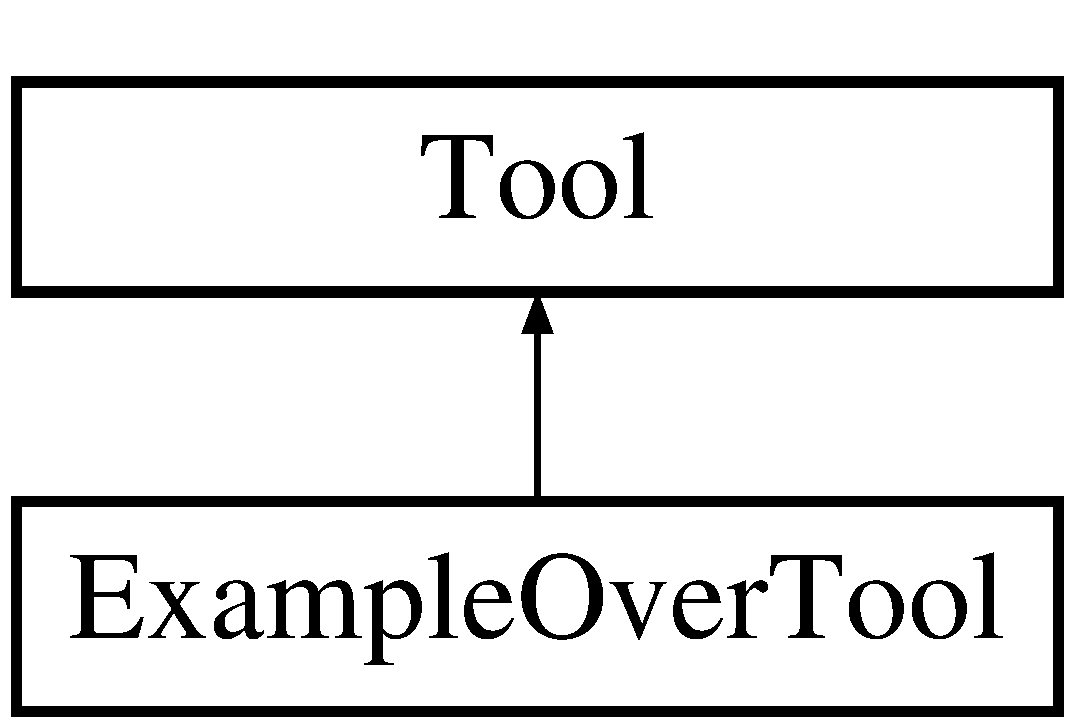
\includegraphics[height=2.000000cm]{classExampleOverTool}
\end{center}
\end{figure}
\subsection*{Public Member Functions}
\begin{DoxyCompactItemize}
\item 
\hypertarget{classExampleOverTool_ac7821b52bdffd736c9f4bb7265f2403c}{bool {\bfseries Initialise} (std\-::string configfile, \hyperlink{classDataModel}{Data\-Model} \&data)}\label{classExampleOverTool_ac7821b52bdffd736c9f4bb7265f2403c}

\item 
\hypertarget{classExampleOverTool_ae43f1902d5b79f6b474ba4b173ab0264}{bool {\bfseries Execute} ()}\label{classExampleOverTool_ae43f1902d5b79f6b474ba4b173ab0264}

\item 
\hypertarget{classExampleOverTool_aaf2c1cee9746ed6e94a9d58d8bc9fcae}{bool {\bfseries Finalise} ()}\label{classExampleOverTool_aaf2c1cee9746ed6e94a9d58d8bc9fcae}

\end{DoxyCompactItemize}


The documentation for this class was generated from the following files\-:\begin{DoxyCompactItemize}
\item 
User\-Tools/\-Examples/Example\-Over\-Tool.\-h\item 
User\-Tools/\-Examples/Example\-Over\-Tool.\-cpp\end{DoxyCompactItemize}

\hypertarget{classExamplePrintData}{\section{Example\-Print\-Data Class Reference}
\label{classExamplePrintData}\index{Example\-Print\-Data@{Example\-Print\-Data}}
}
Inheritance diagram for Example\-Print\-Data\-:\begin{figure}[H]
\begin{center}
\leavevmode
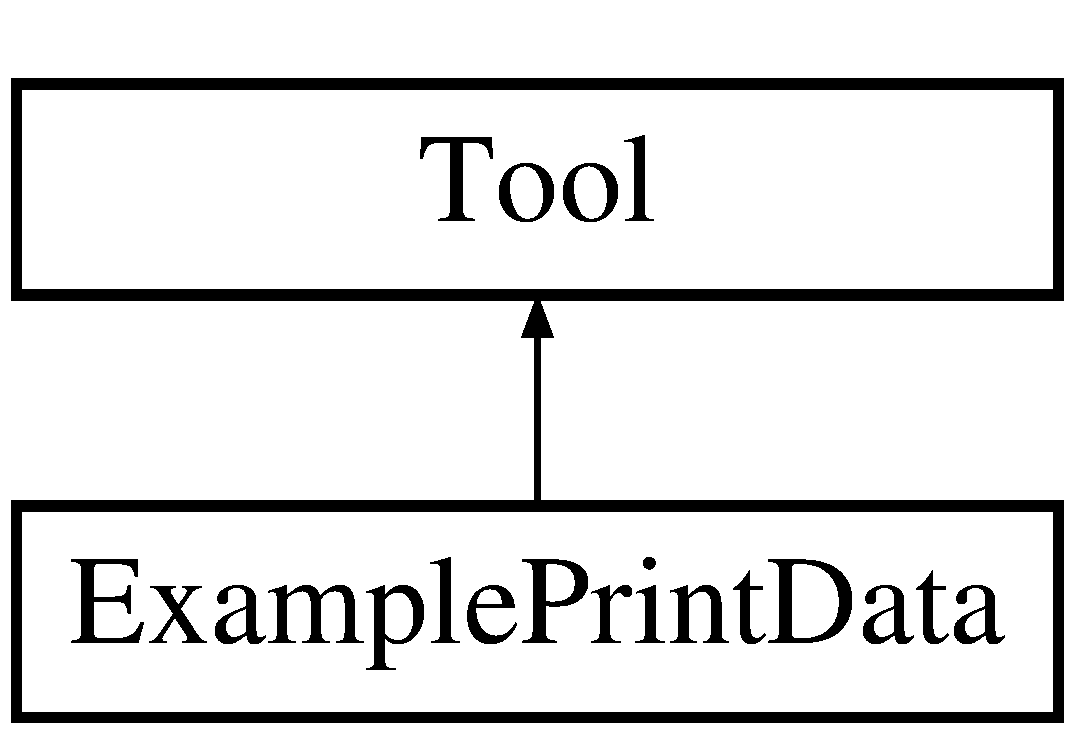
\includegraphics[height=2.000000cm]{classExamplePrintData}
\end{center}
\end{figure}
\subsection*{Public Member Functions}
\begin{DoxyCompactItemize}
\item 
\hypertarget{classExamplePrintData_a307dfd08e3e97a41630506b1796dc89f}{bool {\bfseries Initialise} (std\-::string configfile, \hyperlink{classDataModel}{Data\-Model} \&data)}\label{classExamplePrintData_a307dfd08e3e97a41630506b1796dc89f}

\item 
\hypertarget{classExamplePrintData_aa976e0555bc68a07f9525f556bb51352}{bool {\bfseries Execute} ()}\label{classExamplePrintData_aa976e0555bc68a07f9525f556bb51352}

\item 
\hypertarget{classExamplePrintData_a6b47fdbb41a982a082857c3fd94ac7a9}{bool {\bfseries Finalise} ()}\label{classExamplePrintData_a6b47fdbb41a982a082857c3fd94ac7a9}

\end{DoxyCompactItemize}


The documentation for this class was generated from the following files\-:\begin{DoxyCompactItemize}
\item 
User\-Tools/\-Examples/Example\-Print\-Data.\-h\item 
User\-Tools/\-Examples/Example\-Print\-Data.\-cpp\end{DoxyCompactItemize}

\hypertarget{classExampleRoot}{
\section{ExampleRoot Class Reference}
\label{classExampleRoot}\index{ExampleRoot@{ExampleRoot}}
}
\subsection*{Public Member Functions}
\begin{DoxyCompactItemize}
\item 
\hypertarget{classExampleRoot_a676a00459c76535ea0cc496333e0927f}{
{\bfseries ExampleRoot} (TTree $\ast$tree=0)}
\label{classExampleRoot_a676a00459c76535ea0cc496333e0927f}

\item 
\hypertarget{classExampleRoot_aa76fc5be93bb26800ef2d47b86db68ab}{
virtual Int\_\-t {\bfseries Cut} (Long64\_\-t entry)}
\label{classExampleRoot_aa76fc5be93bb26800ef2d47b86db68ab}

\item 
\hypertarget{classExampleRoot_aeaa244a73538e72d6d4431d6755e6aa9}{
virtual Int\_\-t {\bfseries GetEntry} (Long64\_\-t entry)}
\label{classExampleRoot_aeaa244a73538e72d6d4431d6755e6aa9}

\item 
\hypertarget{classExampleRoot_ad12d04e02467dc4541eaa95c112dfb65}{
virtual Long64\_\-t {\bfseries LoadTree} (Long64\_\-t entry)}
\label{classExampleRoot_ad12d04e02467dc4541eaa95c112dfb65}

\item 
\hypertarget{classExampleRoot_a6a24778d602dc1ecb97f8aeca9c2576c}{
virtual void {\bfseries Init} (TTree $\ast$tree)}
\label{classExampleRoot_a6a24778d602dc1ecb97f8aeca9c2576c}

\item 
\hypertarget{classExampleRoot_ac2cd7b771c6f1094df4278c2c81fa5d4}{
virtual void {\bfseries Loop} ()}
\label{classExampleRoot_ac2cd7b771c6f1094df4278c2c81fa5d4}

\item 
\hypertarget{classExampleRoot_ad2f3d94e1e75887a972eb220e55c6453}{
virtual Bool\_\-t {\bfseries Notify} ()}
\label{classExampleRoot_ad2f3d94e1e75887a972eb220e55c6453}

\item 
\hypertarget{classExampleRoot_ae352817f33d623e4a07ce448bc191533}{
virtual void {\bfseries Show} (Long64\_\-t entry=-\/1)}
\label{classExampleRoot_ae352817f33d623e4a07ce448bc191533}

\end{DoxyCompactItemize}
\subsection*{Public Attributes}
\begin{DoxyCompactItemize}
\item 
\hypertarget{classExampleRoot_a4717cece1b2513740bf12fe1b1f269cc}{
TTree $\ast$ {\bfseries fChain}}
\label{classExampleRoot_a4717cece1b2513740bf12fe1b1f269cc}

\item 
\hypertarget{classExampleRoot_aae45e22777e3dec49bc68fae4850cf63}{
Int\_\-t \hyperlink{classExampleRoot_aae45e22777e3dec49bc68fae4850cf63}{fCurrent}}
\label{classExampleRoot_aae45e22777e3dec49bc68fae4850cf63}

\begin{DoxyCompactList}\small\item\em pointer to the analyzed TTree or TChain \item\end{DoxyCompactList}\item 
\hypertarget{classExampleRoot_a184637f032bbd33058f288c631ad4b08}{
Int\_\-t \hyperlink{classExampleRoot_a184637f032bbd33058f288c631ad4b08}{a}}
\label{classExampleRoot_a184637f032bbd33058f288c631ad4b08}

\begin{DoxyCompactList}\small\item\em current Tree number in a TChain \item\end{DoxyCompactList}\item 
\hypertarget{classExampleRoot_a906499b01132e5c5e9c220ee2e7d75dd}{
Double\_\-t {\bfseries b}}
\label{classExampleRoot_a906499b01132e5c5e9c220ee2e7d75dd}

\item 
\hypertarget{classExampleRoot_aad0a4cee176922682ae2330e1613c978}{
std::string $\ast$ {\bfseries c}}
\label{classExampleRoot_aad0a4cee176922682ae2330e1613c978}

\item 
\hypertarget{classExampleRoot_adbbc71a9b714437196324a5144ba38d6}{
TBranch $\ast$ {\bfseries b\_\-a}}
\label{classExampleRoot_adbbc71a9b714437196324a5144ba38d6}

\item 
\hypertarget{classExampleRoot_a8c1be09581a81eb61c945ee01894f078}{
TBranch $\ast$ {\bfseries b\_\-b}}
\label{classExampleRoot_a8c1be09581a81eb61c945ee01894f078}

\item 
\hypertarget{classExampleRoot_ab3c9727dc708989f36140651ec6a898c}{
TBranch $\ast$ {\bfseries b\_\-c}}
\label{classExampleRoot_ab3c9727dc708989f36140651ec6a898c}

\end{DoxyCompactItemize}
\subsection*{Friends}
\begin{DoxyCompactItemize}
\item 
\hypertarget{classExampleRoot_ac98d07dd8f7b70e16ccb9a01abf56b9c}{
class {\bfseries boost::serialization::access}}
\label{classExampleRoot_ac98d07dd8f7b70e16ccb9a01abf56b9c}

\end{DoxyCompactItemize}


The documentation for this class was generated from the following files:\begin{DoxyCompactItemize}
\item 
DataModel/ExampleRoot.h\item 
DataModel/ExampleRoot.cpp\end{DoxyCompactItemize}

\hypertarget{classExampleSaveRoot}{
\section{ExampleSaveRoot Class Reference}
\label{classExampleSaveRoot}\index{ExampleSaveRoot@{ExampleSaveRoot}}
}
\subsection*{Public Member Functions}
\begin{DoxyCompactItemize}
\item 
\hypertarget{classExampleSaveRoot_a71c138625e281936faa6febe787a4f24}{
bool {\bfseries Initialise} (std::string configfile, \hyperlink{classDataModel}{DataModel} \&data)}
\label{classExampleSaveRoot_a71c138625e281936faa6febe787a4f24}

\item 
\hypertarget{classExampleSaveRoot_a5068a1d780f454298301ee6f26ac4357}{
bool {\bfseries Execute} ()}
\label{classExampleSaveRoot_a5068a1d780f454298301ee6f26ac4357}

\item 
\hypertarget{classExampleSaveRoot_a06f29407ff26756770b6e60eedae8ebf}{
bool {\bfseries Finalise} ()}
\label{classExampleSaveRoot_a06f29407ff26756770b6e60eedae8ebf}

\end{DoxyCompactItemize}


The documentation for this class was generated from the following files:\begin{DoxyCompactItemize}
\item 
UserTools/Examples/ExampleSaveRoot.h\item 
UserTools/Examples/ExampleSaveRoot.cpp\end{DoxyCompactItemize}

\hypertarget{classExampleSaveStore}{\section{Example\-Save\-Store Class Reference}
\label{classExampleSaveStore}\index{Example\-Save\-Store@{Example\-Save\-Store}}
}
Inheritance diagram for Example\-Save\-Store\-:\begin{figure}[H]
\begin{center}
\leavevmode
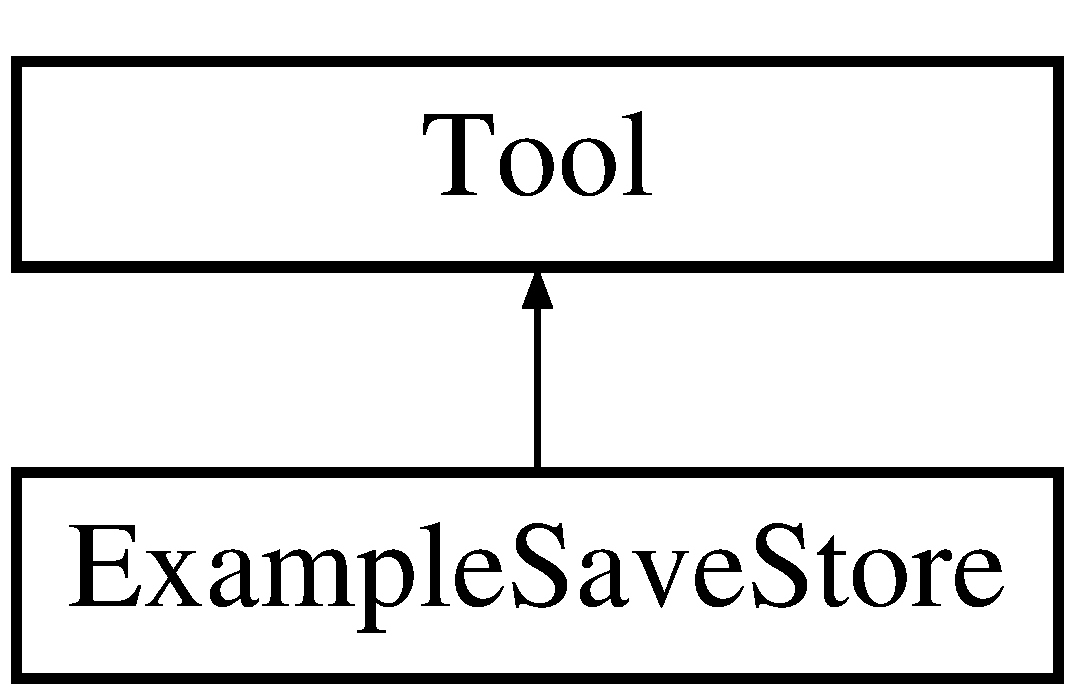
\includegraphics[height=2.000000cm]{classExampleSaveStore}
\end{center}
\end{figure}
\subsection*{Public Member Functions}
\begin{DoxyCompactItemize}
\item 
\hypertarget{classExampleSaveStore_a9c575471c5d024446e7b71b7340cc600}{bool {\bfseries Initialise} (std\-::string configfile, \hyperlink{classDataModel}{Data\-Model} \&data)}\label{classExampleSaveStore_a9c575471c5d024446e7b71b7340cc600}

\item 
\hypertarget{classExampleSaveStore_ab95ccff687c8114d6813a87c2bede948}{bool {\bfseries Execute} ()}\label{classExampleSaveStore_ab95ccff687c8114d6813a87c2bede948}

\item 
\hypertarget{classExampleSaveStore_aa28ea62a5f5bba4c04d271d502859e78}{bool {\bfseries Finalise} ()}\label{classExampleSaveStore_aa28ea62a5f5bba4c04d271d502859e78}

\end{DoxyCompactItemize}


The documentation for this class was generated from the following files\-:\begin{DoxyCompactItemize}
\item 
User\-Tools/\-Examples/Example\-Save\-Store.\-h\item 
User\-Tools/\-Examples/Example\-Save\-Store.\-cpp\end{DoxyCompactItemize}

\hypertarget{classFindMrdTracks}{
\section{FindMrdTracks Class Reference}
\label{classFindMrdTracks}\index{FindMrdTracks@{FindMrdTracks}}
}
\subsection*{Public Member Functions}
\begin{DoxyCompactItemize}
\item 
\hypertarget{classFindMrdTracks_a32cc40daea77e8fc6d4f64791922696e}{
bool {\bfseries Initialise} (std::string configfile, \hyperlink{classDataModel}{DataModel} \&data)}
\label{classFindMrdTracks_a32cc40daea77e8fc6d4f64791922696e}

\item 
\hypertarget{classFindMrdTracks_a24260dbeaee440f91c5aaad0af93886c}{
bool {\bfseries Execute} ()}
\label{classFindMrdTracks_a24260dbeaee440f91c5aaad0af93886c}

\item 
\hypertarget{classFindMrdTracks_a4c03c3790e73938bc9786981de31bab4}{
bool {\bfseries Finalise} ()}
\label{classFindMrdTracks_a4c03c3790e73938bc9786981de31bab4}

\item 
\hypertarget{classFindMrdTracks_acdbbb5dc3f26dcbc527d08483b2bcc9e}{
void {\bfseries StartNewFile} ()}
\label{classFindMrdTracks_acdbbb5dc3f26dcbc527d08483b2bcc9e}

\end{DoxyCompactItemize}


The documentation for this class was generated from the following files:\begin{DoxyCompactItemize}
\item 
UserTools/FindMrdTracks/FindMrdTracks.h\item 
UserTools/FindMrdTracks/FindMrdTracks.cpp\end{DoxyCompactItemize}

\hypertarget{classFindTrackLengthInWater}{\section{Find\-Track\-Length\-In\-Water Class Reference}
\label{classFindTrackLengthInWater}\index{Find\-Track\-Length\-In\-Water@{Find\-Track\-Length\-In\-Water}}
}
Inheritance diagram for Find\-Track\-Length\-In\-Water\-:\begin{figure}[H]
\begin{center}
\leavevmode
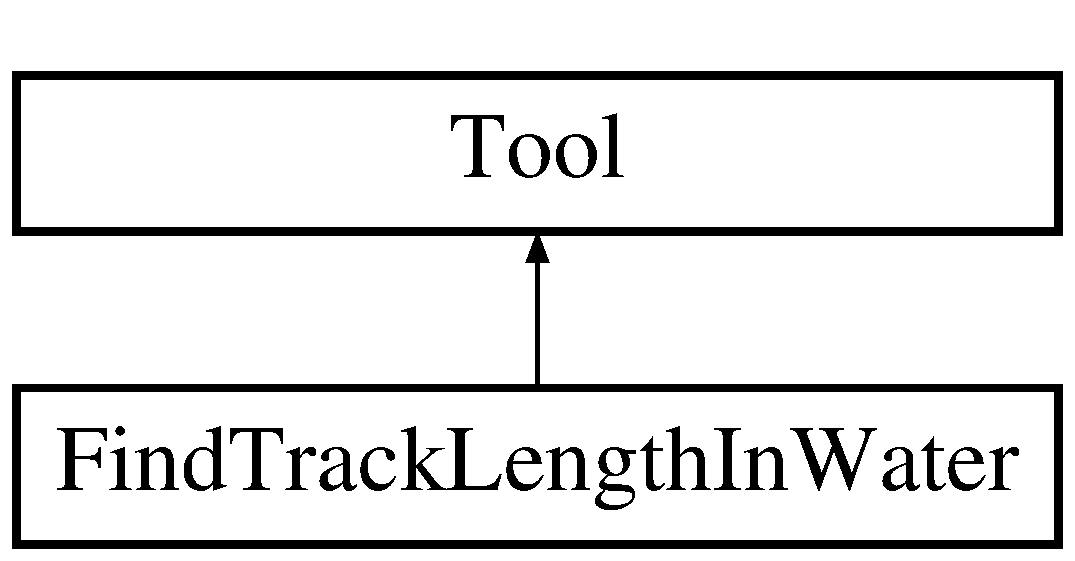
\includegraphics[height=2.000000cm]{classFindTrackLengthInWater}
\end{center}
\end{figure}
\subsection*{Public Member Functions}
\begin{DoxyCompactItemize}
\item 
\hypertarget{classFindTrackLengthInWater_a0f902c566760c2df0693cf00e99cc47e}{bool {\bfseries Initialise} (std\-::string configfile, \hyperlink{classDataModel}{Data\-Model} \&data)}\label{classFindTrackLengthInWater_a0f902c566760c2df0693cf00e99cc47e}

\item 
\hypertarget{classFindTrackLengthInWater_a27d29773eced4222f316ade698247d50}{bool {\bfseries Execute} ()}\label{classFindTrackLengthInWater_a27d29773eced4222f316ade698247d50}

\item 
\hypertarget{classFindTrackLengthInWater_a714975810be358a8b6c127a9b7992dc6}{double {\bfseries find\-\_\-lambda} (double xmu\-\_\-rec, double ymu\-\_\-rec, double zmu\-\_\-rec, double xrec\-Dir, double yrec\-Dir, double zrec\-Dir, double x\-\_\-pmtpos, double y\-\_\-pmtpos, double z\-\_\-pmtpos, double theta\-\_\-cher)}\label{classFindTrackLengthInWater_a714975810be358a8b6c127a9b7992dc6}

\item 
\hypertarget{classFindTrackLengthInWater_a1e9e6eaefc14833736544ebffb39eb1c}{bool {\bfseries Finalise} ()}\label{classFindTrackLengthInWater_a1e9e6eaefc14833736544ebffb39eb1c}

\end{DoxyCompactItemize}


The documentation for this class was generated from the following files\-:\begin{DoxyCompactItemize}
\item 
User\-Tools/\-Find\-Track\-Length\-In\-Water/Find\-Track\-Length\-In\-Water.\-h\item 
User\-Tools/\-Find\-Track\-Length\-In\-Water/Find\-Track\-Length\-In\-Water.\-cpp\end{DoxyCompactItemize}

\hypertarget{classFoMCalculator}{\section{Fo\-M\-Calculator Class Reference}
\label{classFoMCalculator}\index{Fo\-M\-Calculator@{Fo\-M\-Calculator}}
}
\subsection*{Public Member Functions}
\begin{DoxyCompactItemize}
\item 
\hypertarget{classFoMCalculator_a08e7a4cf1cbdeca75bde8d3c783eb543}{void {\bfseries Set\-Time\-Fit\-Weight} (double tweight)}\label{classFoMCalculator_a08e7a4cf1cbdeca75bde8d3c783eb543}

\item 
\hypertarget{classFoMCalculator_a7b70fa75561ef8047f4851e3572bea88}{void {\bfseries Set\-Cone\-Fit\-Weight} (double cweight)}\label{classFoMCalculator_a7b70fa75561ef8047f4851e3572bea88}

\item 
\hypertarget{classFoMCalculator_a410023f27226ff81d1c1f0c6d20d8121}{void {\bfseries Set\-Mean\-Time\-Calculator\-Type} (int type)}\label{classFoMCalculator_a410023f27226ff81d1c1f0c6d20d8121}

\item 
\hypertarget{classFoMCalculator_aa6a0ef5f03186fc3722f785104199abd}{void {\bfseries Load\-Vertex\-Geometry} (\hyperlink{classVertexGeometry}{Vertex\-Geometry} $\ast$vtxgeo)}\label{classFoMCalculator_aa6a0ef5f03186fc3722f785104199abd}

\item 
\hypertarget{classFoMCalculator_afc907bb278a95071410be7d0337253a1}{double {\bfseries Find\-Simple\-Time\-Properties} (double my\-Cone\-Edge)}\label{classFoMCalculator_afc907bb278a95071410be7d0337253a1}

\item 
\hypertarget{classFoMCalculator_ad62643573ab780bf3329d0c48f615c7a}{void {\bfseries Time\-Properties\-Ln\-L} (double vtx\-Time, double \&vtx\-Fom)}\label{classFoMCalculator_ad62643573ab780bf3329d0c48f615c7a}

\item 
\hypertarget{classFoMCalculator_a8697cdce3d92b4c8afb843b4e20ae0cd}{void {\bfseries Cone\-Properties\-Fo\-M} (double cone\-Edge, double \&chi2)}\label{classFoMCalculator_a8697cdce3d92b4c8afb843b4e20ae0cd}

\item 
\hypertarget{classFoMCalculator_a14d1020216db6fc5149b7918e8138b0b}{void {\bfseries Point\-Position\-Chi2} (double vtx\-X, double vtx\-Y, double vtx\-Z, double vtx\-Time, double \&fom)}\label{classFoMCalculator_a14d1020216db6fc5149b7918e8138b0b}

\item 
\hypertarget{classFoMCalculator_a275afaff36e1d93e732811382c433566}{void {\bfseries Point\-Direction\-Chi2} (double vtx\-X, double vtx\-Y, double vtx\-Z, double dir\-X, double dir\-Y, double dir\-Z, double cone\-Angle, double \&fom)}\label{classFoMCalculator_a275afaff36e1d93e732811382c433566}

\item 
\hypertarget{classFoMCalculator_a6fc036ee8918755886ffa842e5c5d781}{void {\bfseries Point\-Vertex\-Chi2} (double vtx\-X, double vtx\-Y, double vtx\-Z, double dir\-X, double dir\-Y, double dir\-Z, double cone\-Angle, double vtx\-Time, double \&fom)}\label{classFoMCalculator_a6fc036ee8918755886ffa842e5c5d781}

\item 
\hypertarget{classFoMCalculator_a419589ed8639a623dec06684e57d0db5}{void {\bfseries Extended\-Vertex\-Chi2} (double vtx\-X, double vtx\-Y, double vtx\-Z, double dir\-X, double dir\-Y, double dir\-Z, double cone\-Angle, double vtx\-Time, double \&fom)}\label{classFoMCalculator_a419589ed8639a623dec06684e57d0db5}

\end{DoxyCompactItemize}
\subsection*{Public Attributes}
\begin{DoxyCompactItemize}
\item 
\hypertarget{classFoMCalculator_a3a7bca0306b8b1570e639b863ed7e92e}{double {\bfseries f\-Base\-F\-O\-M}}\label{classFoMCalculator_a3a7bca0306b8b1570e639b863ed7e92e}

\item 
\hypertarget{classFoMCalculator_ae9c9449bfa160d8c5d241ab3b729a10b}{double {\bfseries f\-Time\-Fit\-Weight}}\label{classFoMCalculator_ae9c9449bfa160d8c5d241ab3b729a10b}

\item 
\hypertarget{classFoMCalculator_a74a5ae95c46e77c0d70f346ddf5ac7b4}{double {\bfseries f\-Cone\-Fit\-Weight}}\label{classFoMCalculator_a74a5ae95c46e77c0d70f346ddf5ac7b4}

\item 
\hypertarget{classFoMCalculator_ae80b01958ac5f9513b46406ac46ac486}{int {\bfseries f\-Mean\-Time\-Calculator\-Type}}\label{classFoMCalculator_ae80b01958ac5f9513b46406ac46ac486}

\item 
\hypertarget{classFoMCalculator_a8962e8746e1e5a857c73c1d3c2b350ee}{\hyperlink{classVertexGeometry}{Vertex\-Geometry} $\ast$ {\bfseries f\-Vtx\-Geo}}\label{classFoMCalculator_a8962e8746e1e5a857c73c1d3c2b350ee}

\end{DoxyCompactItemize}


The documentation for this class was generated from the following files\-:\begin{DoxyCompactItemize}
\item 
Data\-Model/Fo\-M\-Calculator.\-h\item 
Data\-Model/Fo\-M\-Calculator.\-cpp\end{DoxyCompactItemize}

\hypertarget{classGenerateHits}{
\section{GenerateHits Class Reference}
\label{classGenerateHits}\index{GenerateHits@{GenerateHits}}
}
\subsection*{Public Member Functions}
\begin{DoxyCompactItemize}
\item 
\hypertarget{classGenerateHits_a11c98b7819edf56f56d1981b72ed9e24}{
bool {\bfseries Initialise} (std::string configfile, \hyperlink{classDataModel}{DataModel} \&data)}
\label{classGenerateHits_a11c98b7819edf56f56d1981b72ed9e24}

\item 
\hypertarget{classGenerateHits_a3bf8e799c8fd096b2b3e802693fc043d}{
bool {\bfseries Execute} ()}
\label{classGenerateHits_a3bf8e799c8fd096b2b3e802693fc043d}

\item 
\hypertarget{classGenerateHits_a2c84756b951a63d38a6601a61334895d}{
bool {\bfseries Finalise} ()}
\label{classGenerateHits_a2c84756b951a63d38a6601a61334895d}

\item 
\hypertarget{classGenerateHits_ae875934539804dd522f826c7d14e4bca}{
double {\bfseries fRand} (double fMin, double fMax)}
\label{classGenerateHits_ae875934539804dd522f826c7d14e4bca}

\end{DoxyCompactItemize}


The documentation for this class was generated from the following files:\begin{DoxyCompactItemize}
\item 
UserTools/GenerateHits/GenerateHits.h\item 
UserTools/GenerateHits/GenerateHits.cpp\end{DoxyCompactItemize}

\hypertarget{classGeometry}{\section{Geometry Class Reference}
\label{classGeometry}\index{Geometry@{Geometry}}
}
Inheritance diagram for Geometry\-:\begin{figure}[H]
\begin{center}
\leavevmode
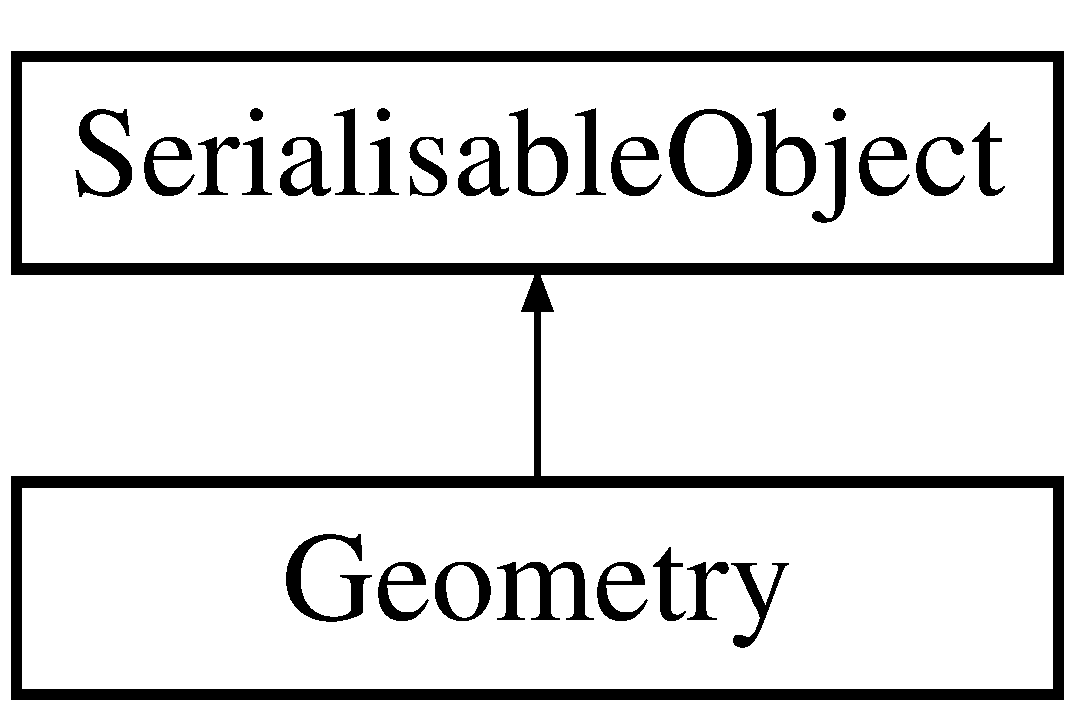
\includegraphics[height=2.000000cm]{classGeometry}
\end{center}
\end{figure}
\subsection*{Public Member Functions}
\begin{DoxyCompactItemize}
\item 
\hypertarget{classGeometry_ab5170692a6cbe471976e851f79e9319a}{Real\-Detectors {\bfseries reserve} (10)}\label{classGeometry_ab5170692a6cbe471976e851f79e9319a}

\item 
\hypertarget{classGeometry_a6f68b0647ccbaf76ba714730451dc3cf}{{\bfseries Geometry} (double ver, \hyperlink{classPosition}{Position} tankc, double tankr, double tankhh, double pmtencr, double pmtenchh, double mrdw, double mrdh, double mrdd, double mrds, int ntankpmts, int nmrdpmts, int nvetopmts, int nlappds, geostatus statin, std\-::vector$<$ std\-::map$<$ unsigned long, \hyperlink{classDetector}{Detector} $>$ $\ast$ $>$dets=std\-::vector$<$ std\-::map$<$ unsigned long, \hyperlink{classDetector}{Detector} $>$ $\ast$ $>$\{\})}\label{classGeometry_a6f68b0647ccbaf76ba714730451dc3cf}

\item 
\hypertarget{classGeometry_afbfabb07e8f8cad1496e2b69db8addb8}{std\-::vector$<$ std\-::map\\*
$<$ unsigned long, \hyperlink{classDetector}{Detector} $>$ $\ast$ $>$ $\ast$ {\bfseries Get\-Detectors} ()}\label{classGeometry_afbfabb07e8f8cad1496e2b69db8addb8}

\item 
\hypertarget{classGeometry_a94c52a826664f141dd3246fa1478a475}{double {\bfseries Get\-Version} ()}\label{classGeometry_a94c52a826664f141dd3246fa1478a475}

\item 
\hypertarget{classGeometry_a21835bb3d23fd54895350c84471dfb02}{geostatus {\bfseries Get\-Status} ()}\label{classGeometry_a21835bb3d23fd54895350c84471dfb02}

\item 
\hypertarget{classGeometry_a804b7ce9d8f1abe1ce5fffe9da65af51}{\hyperlink{classPosition}{Position} {\bfseries Get\-Tank\-Centre} ()}\label{classGeometry_a804b7ce9d8f1abe1ce5fffe9da65af51}

\item 
\hypertarget{classGeometry_abc3f55a2c64ec9f83a0ea7e82724fe49}{double {\bfseries Get\-Tank\-Radius} ()}\label{classGeometry_abc3f55a2c64ec9f83a0ea7e82724fe49}

\item 
\hypertarget{classGeometry_acc0459993448786f92dbdad8c4652176}{double {\bfseries Get\-Tank\-Halfheight} ()}\label{classGeometry_acc0459993448786f92dbdad8c4652176}

\item 
\hypertarget{classGeometry_abd765c4d73ceba92e39d007b6c3362bd}{double {\bfseries Get\-P\-M\-T\-Enclosed\-Radius} ()}\label{classGeometry_abd765c4d73ceba92e39d007b6c3362bd}

\item 
\hypertarget{classGeometry_a42b716a80c24a5278099e7ae8515dd69}{double {\bfseries Get\-P\-M\-T\-Enclosed\-Halfheight} ()}\label{classGeometry_a42b716a80c24a5278099e7ae8515dd69}

\item 
\hypertarget{classGeometry_ad33910b8b84b8956ecbfa4954a7ccfcc}{double {\bfseries Get\-Fiducial\-Cut\-Radius} ()}\label{classGeometry_ad33910b8b84b8956ecbfa4954a7ccfcc}

\item 
\hypertarget{classGeometry_a849d59159bc9afef2fb5a5de1b8f920d}{double {\bfseries Get\-Fiducial\-Cut\-Y} ()}\label{classGeometry_a849d59159bc9afef2fb5a5de1b8f920d}

\item 
\hypertarget{classGeometry_a858a7eafaa3c0629e596d1abf3e9346b}{double {\bfseries Get\-Fiducial\-Cut\-Z} ()}\label{classGeometry_a858a7eafaa3c0629e596d1abf3e9346b}

\item 
\hypertarget{classGeometry_a7dc78bc77bd7e01df60c513e3c1f3a8d}{double {\bfseries Get\-Mrd\-Width} ()}\label{classGeometry_a7dc78bc77bd7e01df60c513e3c1f3a8d}

\item 
\hypertarget{classGeometry_ad89709f6efbf3119c90da8e7631e1024}{double {\bfseries Get\-Mrd\-Height} ()}\label{classGeometry_ad89709f6efbf3119c90da8e7631e1024}

\item 
\hypertarget{classGeometry_a867b5607dbd4d3baeed4f03317026af5}{double {\bfseries Get\-Mrd\-Depth} ()}\label{classGeometry_a867b5607dbd4d3baeed4f03317026af5}

\item 
\hypertarget{classGeometry_a43cefba896c4f17a1607b658ae81c47d}{double {\bfseries Get\-Mrd\-Start} ()}\label{classGeometry_a43cefba896c4f17a1607b658ae81c47d}

\item 
\hypertarget{classGeometry_a61a5beb5c95207de729dddb94670ad55}{double {\bfseries Get\-Mrd\-End} ()}\label{classGeometry_a61a5beb5c95207de729dddb94670ad55}

\item 
\hypertarget{classGeometry_afdc0b24374cc8906be35ea93d1c99520}{void {\bfseries Set\-Version} (double Version\-In)}\label{classGeometry_afdc0b24374cc8906be35ea93d1c99520}

\item 
\hypertarget{classGeometry_a2ecdbc2a94b827fa0c372da34138d77f}{void {\bfseries Set\-Status} (geostatus Status\-In)}\label{classGeometry_a2ecdbc2a94b827fa0c372da34138d77f}

\item 
\hypertarget{classGeometry_ac333cb9fd34843161769b5eaf084219f}{void {\bfseries Set\-Tank\-Centre} (\hyperlink{classPosition}{Position} tank\-\_\-centrein)}\label{classGeometry_ac333cb9fd34843161769b5eaf084219f}

\item 
\hypertarget{classGeometry_a0f2d050fa42af21e6e0b4914974b45f5}{void {\bfseries Set\-Tank\-Radius} (double tank\-\_\-radius\-In)}\label{classGeometry_a0f2d050fa42af21e6e0b4914974b45f5}

\item 
\hypertarget{classGeometry_aae1817255945967705d105665b2fb248}{void {\bfseries Set\-Tank\-Halfheight} (double tank\-\_\-halfheight\-In)}\label{classGeometry_aae1817255945967705d105665b2fb248}

\item 
\hypertarget{classGeometry_a220d86cc649f42a16d33c73c1fc9e70e}{void {\bfseries Set\-P\-M\-T\-Enclosed\-Radius} (double pmt\-\_\-enclosed\-\_\-radius\-In)}\label{classGeometry_a220d86cc649f42a16d33c73c1fc9e70e}

\item 
\hypertarget{classGeometry_aca093a4eaad96fa51b4bac6fbe5fc5b6}{void {\bfseries Set\-P\-M\-T\-Enclosed\-Halfheight} (double pmt\-\_\-enclosed\-\_\-halfheight\-In)}\label{classGeometry_aca093a4eaad96fa51b4bac6fbe5fc5b6}

\item 
\hypertarget{classGeometry_a88cbe634b7185c5230f925a182599dd1}{void {\bfseries Set\-Fiducial\-Cut\-Radius} (double fidcutradiusin)}\label{classGeometry_a88cbe634b7185c5230f925a182599dd1}

\item 
\hypertarget{classGeometry_acddde32956d96095d3deb2d00c90a3ee}{void {\bfseries Set\-Fiducial\-Cut\-Z} (double fidcutzin)}\label{classGeometry_acddde32956d96095d3deb2d00c90a3ee}

\item 
\hypertarget{classGeometry_a808167f759b49e7958abe1598d6b6294}{void {\bfseries Set\-Fiducial\-Cut\-Y} (double fidcutyin)}\label{classGeometry_a808167f759b49e7958abe1598d6b6294}

\item 
\hypertarget{classGeometry_a120524e0dcd97fdea137b49b976a5183}{void {\bfseries Set\-Mrd\-Width} (double mrd\-\_\-width\-In)}\label{classGeometry_a120524e0dcd97fdea137b49b976a5183}

\item 
\hypertarget{classGeometry_a42377661ec147b299c500e9aa49aaf54}{void {\bfseries Set\-Mrd\-Height} (double mrd\-\_\-height\-In)}\label{classGeometry_a42377661ec147b299c500e9aa49aaf54}

\item 
\hypertarget{classGeometry_a44da646292c6c7e83709e8aa47236844}{void {\bfseries Set\-Mrd\-Depth} (double mrd\-\_\-depth\-In)}\label{classGeometry_a44da646292c6c7e83709e8aa47236844}

\item 
\hypertarget{classGeometry_a100d585e24c6c52794741e280d4dd4c6}{void {\bfseries Set\-Mrd\-Start} (double mrd\-\_\-start\-In)}\label{classGeometry_a100d585e24c6c52794741e280d4dd4c6}

\item 
\hypertarget{classGeometry_a2543a2a6d20336cc25a26fba69245955}{void {\bfseries Set\-Detectors} (std\-::vector$<$ std\-::map$<$ unsigned long, \hyperlink{classDetector}{Detector} $>$ $\ast$ $>$Detectors\-In)}\label{classGeometry_a2543a2a6d20336cc25a26fba69245955}

\item 
\hypertarget{classGeometry_ac5f3c966b7862b10af20fb83c9c45082}{unsigned long {\bfseries Consume\-Next\-Free\-Channel\-Key} ()}\label{classGeometry_ac5f3c966b7862b10af20fb83c9c45082}

\item 
\hypertarget{classGeometry_aea3868f7e8a725f672a2e488fe95eb5f}{unsigned long {\bfseries Consume\-Next\-Free\-Detector\-Key} ()}\label{classGeometry_aea3868f7e8a725f672a2e488fe95eb5f}

\item 
\hypertarget{classGeometry_aedc8d0b00db707eb63177b3fbc55e7f7}{bool {\bfseries Add\-Detector} (\hyperlink{classDetector}{Detector} detin)}\label{classGeometry_aedc8d0b00db707eb63177b3fbc55e7f7}

\item 
\hypertarget{classGeometry_a9c164587d17b71fb8cbcfa0535dca18f}{int {\bfseries Get\-Num\-Detectors} ()}\label{classGeometry_a9c164587d17b71fb8cbcfa0535dca18f}

\item 
\hypertarget{classGeometry_a3b4131297b0329603c7700e7eed9cf0b}{\hyperlink{classDetector}{Detector} $\ast$ {\bfseries Get\-Detector} (unsigned long Detector\-Key)}\label{classGeometry_a3b4131297b0329603c7700e7eed9cf0b}

\item 
\hypertarget{classGeometry_a6091d6b92a17207fdda50a03cc64b381}{\hyperlink{classDetector}{Detector} $\ast$ {\bfseries Channel\-To\-Detector} (unsigned long \hyperlink{classChannelKey}{Channel\-Key})}\label{classGeometry_a6091d6b92a17207fdda50a03cc64b381}

\item 
\hypertarget{classGeometry_a68873d502689bb73337c3f8d6e0ef3bf}{\hyperlink{classChannel}{Channel} $\ast$ {\bfseries Get\-Channel} (unsigned long \hyperlink{classChannelKey}{Channel\-Key})}\label{classGeometry_a68873d502689bb73337c3f8d6e0ef3bf}

\item 
\hypertarget{classGeometry_a60e84520417769401492de9e182636fc}{void {\bfseries Init\-Channel\-Map} ()}\label{classGeometry_a60e84520417769401492de9e182636fc}

\item 
\hypertarget{classGeometry_a4354935089665d2856b9a9a5bb1f181a}{int {\bfseries Get\-Num\-Detectors\-In\-Set} (std\-::string Set\-Name)}\label{classGeometry_a4354935089665d2856b9a9a5bb1f181a}

\item 
\hypertarget{classGeometry_aca1dd1c2919c14b2d8bdf40db23c5ba9}{bool {\bfseries Get\-Tank\-Contained} (\hyperlink{classParticle}{Particle} part, int startstop=0)}\label{classGeometry_aca1dd1c2919c14b2d8bdf40db23c5ba9}

\item 
\hypertarget{classGeometry_a2c68539bcaaf45158dbcdc50c3f65ca6}{bool {\bfseries Get\-Tank\-Contained} (\hyperlink{classPosition}{Position} a\-Vertex)}\label{classGeometry_a2c68539bcaaf45158dbcdc50c3f65ca6}

\item 
\hypertarget{classGeometry_af4c8b8f5df92cf905e0ea7098ceb52ed}{bool {\bfseries Get\-Mrd\-Contained} (\hyperlink{classParticle}{Particle} part, int startstop=0)}\label{classGeometry_af4c8b8f5df92cf905e0ea7098ceb52ed}

\item 
\hypertarget{classGeometry_a9da73da227027f3592e9ef10cb06033f}{bool {\bfseries Get\-Mrd\-Contained} (\hyperlink{classPosition}{Position} a\-Vertex)}\label{classGeometry_a9da73da227027f3592e9ef10cb06033f}

\item 
\hypertarget{classGeometry_a5ddd7d7d95f76d8d711c9727824020ca}{bool {\bfseries Print} ()}\label{classGeometry_a5ddd7d7d95f76d8d711c9727824020ca}

\item 
\hypertarget{classGeometry_acf8cf2161abe0c73a4f285f66277f2cd}{bool {\bfseries Print\-Status} (geostatus status)}\label{classGeometry_acf8cf2161abe0c73a4f285f66277f2cd}

\item 
\hypertarget{classGeometry_a12b34f2e75cdee8441008d9de7e2eb1b}{void {\bfseries Print\-Channels} ()}\label{classGeometry_a12b34f2e75cdee8441008d9de7e2eb1b}

\item 
\hypertarget{classGeometry_af1ef26f91bb256a2a7d52c37f502acc7}{\hyperlink{classPosition}{Position} {\bfseries Global\-To\-Tank\-Centered} (\hyperlink{classPosition}{Position} posin)}\label{classGeometry_af1ef26f91bb256a2a7d52c37f502acc7}

\item 
\hypertarget{classGeometry_a89335cdbf640744d7e4362d8495b6859}{void {\bfseries Cartesian\-To\-Polar} (\hyperlink{classPosition}{Position} posin, double \&R, double \&Phi, double \&Theta, bool tankcentered=false)}\label{classGeometry_a89335cdbf640744d7e4362d8495b6859}

\end{DoxyCompactItemize}
\subsection*{Friends}
\begin{DoxyCompactItemize}
\item 
\hypertarget{classGeometry_ac98d07dd8f7b70e16ccb9a01abf56b9c}{class {\bfseries boost\-::serialization\-::access}}\label{classGeometry_ac98d07dd8f7b70e16ccb9a01abf56b9c}

\end{DoxyCompactItemize}


The documentation for this class was generated from the following files\-:\begin{DoxyCompactItemize}
\item 
Data\-Model/Geometry.\-h\item 
Data\-Model/Geometry.\-cpp\end{DoxyCompactItemize}

\include{classGracefulStop}
\hypertarget{classHeftyInfo}{
\section{HeftyInfo Class Reference}
\label{classHeftyInfo}\index{HeftyInfo@{HeftyInfo}}
}
Inheritance diagram for HeftyInfo::\begin{figure}[H]
\begin{center}
\leavevmode
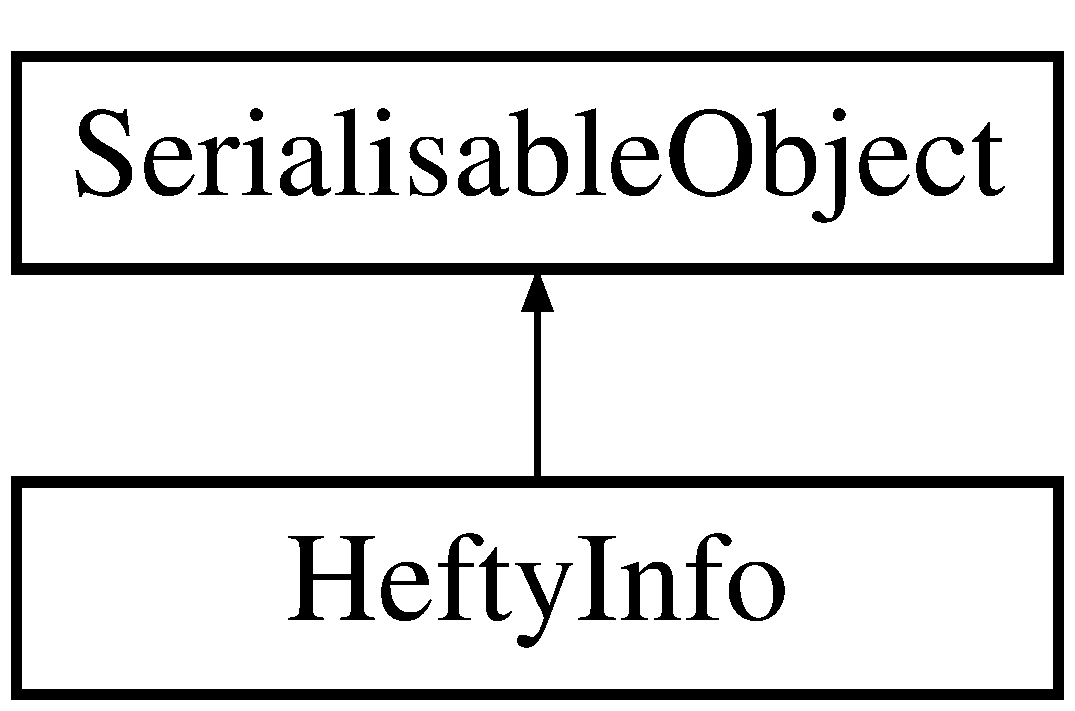
\includegraphics[height=2cm]{classHeftyInfo}
\end{center}
\end{figure}
\subsection*{Public Member Functions}
\begin{DoxyCompactItemize}
\item 
\hypertarget{classHeftyInfo_af721faddd429a02ea7651108185ec478}{
{\bfseries HeftyInfo} (int sequence\_\-id, const std::vector$<$ unsigned long long $>$ \&time, const std::vector$<$ int $>$ \&label, const std::vector$<$ long long $>$ \&t\_\-since\_\-beam, const std::vector$<$ int $>$ \&more)}
\label{classHeftyInfo_af721faddd429a02ea7651108185ec478}

\item 
\hypertarget{classHeftyInfo_a1e9b9d3197a8df5bff0432f1f814109b}{
size\_\-t {\bfseries num\_\-minibuffers} () const }
\label{classHeftyInfo_a1e9b9d3197a8df5bff0432f1f814109b}

\item 
\hypertarget{classHeftyInfo_ab9b5565e7b54b73eb83fd72c3e10a349}{
int {\bfseries sequence\_\-id} () const }
\label{classHeftyInfo_ab9b5565e7b54b73eb83fd72c3e10a349}

\item 
\hypertarget{classHeftyInfo_a9da6b668891f3a104f5fe6b5026e0969}{
unsigned long long {\bfseries time} (size\_\-t mb) const }
\label{classHeftyInfo_a9da6b668891f3a104f5fe6b5026e0969}

\item 
\hypertarget{classHeftyInfo_a2455de20fa2e072b68f58f37307c1989}{
int {\bfseries label} (size\_\-t mb) const }
\label{classHeftyInfo_a2455de20fa2e072b68f58f37307c1989}

\item 
\hypertarget{classHeftyInfo_a6880deb111e4b3f3d1d0bf0be8e4290e}{
long long {\bfseries t\_\-since\_\-beam} (size\_\-t mb) const }
\label{classHeftyInfo_a6880deb111e4b3f3d1d0bf0be8e4290e}

\item 
\hypertarget{classHeftyInfo_abb3cfed8ce0e9d03024d62a5687746cc}{
bool {\bfseries more} () const }
\label{classHeftyInfo_abb3cfed8ce0e9d03024d62a5687746cc}

\item 
\hypertarget{classHeftyInfo_a9f6297619ba660d09a294ad599d3273e}{
std::vector$<$ unsigned long long $>$ {\bfseries all\_\-times} () const }
\label{classHeftyInfo_a9f6297619ba660d09a294ad599d3273e}

\item 
\hypertarget{classHeftyInfo_a4184a22ba444cbfcc94b95bc5b0df49b}{
virtual bool {\bfseries Print} () override}
\label{classHeftyInfo_a4184a22ba444cbfcc94b95bc5b0df49b}

\end{DoxyCompactItemize}
\subsection*{Protected Member Functions}
\begin{DoxyCompactItemize}
\item 
\hypertarget{classHeftyInfo_ae49337fd12c7bd8d0151953aff75a613}{
{\footnotesize template$<$class Archive $>$ }\\void {\bfseries serialize} (Archive \&ar, const unsigned int version)}
\label{classHeftyInfo_ae49337fd12c7bd8d0151953aff75a613}

\end{DoxyCompactItemize}
\subsection*{Protected Attributes}
\begin{DoxyCompactItemize}
\item 
\hypertarget{classHeftyInfo_a0dab6f58a2c3719e087bc18b6e32e528}{
int {\bfseries sequence\_\-id\_\-}}
\label{classHeftyInfo_a0dab6f58a2c3719e087bc18b6e32e528}

\item 
\hypertarget{classHeftyInfo_a49dcdefaf94072a936aaba0f4d335b7b}{
std::vector$<$ unsigned long long $>$ {\bfseries time\_\-}}
\label{classHeftyInfo_a49dcdefaf94072a936aaba0f4d335b7b}

\item 
\hypertarget{classHeftyInfo_a8c18908b972555f6da8137ff67124eaf}{
std::vector$<$ int $>$ {\bfseries label\_\-}}
\label{classHeftyInfo_a8c18908b972555f6da8137ff67124eaf}

\item 
\hypertarget{classHeftyInfo_a68c89d555a59e08992862804591d4876}{
std::vector$<$ long long $>$ {\bfseries t\_\-since\_\-beam\_\-}}
\label{classHeftyInfo_a68c89d555a59e08992862804591d4876}

\item 
\hypertarget{classHeftyInfo_a800c1fb5443ae90314bd670e88d0afd9}{
bool {\bfseries more\_\-}}
\label{classHeftyInfo_a800c1fb5443ae90314bd670e88d0afd9}

\end{DoxyCompactItemize}
\subsection*{Friends}
\begin{DoxyCompactItemize}
\item 
\hypertarget{classHeftyInfo_ac98d07dd8f7b70e16ccb9a01abf56b9c}{
class {\bfseries boost::serialization::access}}
\label{classHeftyInfo_ac98d07dd8f7b70e16ccb9a01abf56b9c}

\end{DoxyCompactItemize}


The documentation for this class was generated from the following file:\begin{DoxyCompactItemize}
\item 
DataModel/HeftyInfo.h\end{DoxyCompactItemize}

\hypertarget{classannie_1_1HeftyTreeReader}{
\section{annie::HeftyTreeReader Class Reference}
\label{classannie_1_1HeftyTreeReader}\index{annie::HeftyTreeReader@{annie::HeftyTreeReader}}
}
\subsection*{Public Member Functions}
\begin{DoxyCompactItemize}
\item 
\hypertarget{classannie_1_1HeftyTreeReader_ac15660ea2670e502c68bc9f80793ae23}{
{\bfseries HeftyTreeReader} (const std::string \&file\_\-name)}
\label{classannie_1_1HeftyTreeReader_ac15660ea2670e502c68bc9f80793ae23}

\item 
\hypertarget{classannie_1_1HeftyTreeReader_a70c65b445f31d18c7ce8c60bd67f2a62}{
{\bfseries HeftyTreeReader} (const std::vector$<$ std::string $>$ \&file\_\-names)}
\label{classannie_1_1HeftyTreeReader_a70c65b445f31d18c7ce8c60bd67f2a62}

\item 
\hypertarget{classannie_1_1HeftyTreeReader_ab82488607c07679869f478b9ec7d88c7}{
{\bfseries HeftyTreeReader} (TChain $\ast$inputChain)}
\label{classannie_1_1HeftyTreeReader_ab82488607c07679869f478b9ec7d88c7}

\item 
\hypertarget{classannie_1_1HeftyTreeReader_a370da5616b748d31cedf3063769de5db}{
std::unique\_\-ptr$<$ \hyperlink{classHeftyInfo}{HeftyInfo} $>$ {\bfseries next} ()}
\label{classannie_1_1HeftyTreeReader_a370da5616b748d31cedf3063769de5db}

\item 
\hypertarget{classannie_1_1HeftyTreeReader_a385017d9b438fc2118be8e67f5a8b7ac}{
std::unique\_\-ptr$<$ \hyperlink{classHeftyInfo}{HeftyInfo} $>$ {\bfseries previous} ()}
\label{classannie_1_1HeftyTreeReader_a385017d9b438fc2118be8e67f5a8b7ac}

\end{DoxyCompactItemize}
\subsection*{Protected Member Functions}
\begin{DoxyCompactItemize}
\item 
\hypertarget{classannie_1_1HeftyTreeReader_a96aa45bd0418dd809a9b5b30f1b0d1c2}{
void {\bfseries set\_\-branch\_\-addresses} ()}
\label{classannie_1_1HeftyTreeReader_a96aa45bd0418dd809a9b5b30f1b0d1c2}

\item 
\hypertarget{classannie_1_1HeftyTreeReader_aeaabddbcd009a65cf22f45dc3b7d4650}{
std::unique\_\-ptr$<$ \hyperlink{classHeftyInfo}{HeftyInfo} $>$ {\bfseries load\_\-next\_\-entry} (bool reverse)}
\label{classannie_1_1HeftyTreeReader_aeaabddbcd009a65cf22f45dc3b7d4650}

\end{DoxyCompactItemize}
\subsection*{Protected Attributes}
\begin{DoxyCompactItemize}
\item 
\hypertarget{classannie_1_1HeftyTreeReader_a2f6016952ec8fc83955a081115eb2cb5}{
TChain {\bfseries hefty\_\-db\_\-chain\_\-}}
\label{classannie_1_1HeftyTreeReader_a2f6016952ec8fc83955a081115eb2cb5}

\item 
\hypertarget{classannie_1_1HeftyTreeReader_a4e71c6e864c27fe549da00eb42d0aff0}{
long long {\bfseries current\_\-hefty\_\-db\_\-entry\_\-} = -\/1}
\label{classannie_1_1HeftyTreeReader_a4e71c6e864c27fe549da00eb42d0aff0}

\item 
\hypertarget{classannie_1_1HeftyTreeReader_ae8a407035678cd910f1a5a6a7ccef830}{
long long \hyperlink{classannie_1_1HeftyTreeReader_ae8a407035678cd910f1a5a6a7ccef830}{last\_\-sequence\_\-id\_\-} = -\/1}
\label{classannie_1_1HeftyTreeReader_ae8a407035678cd910f1a5a6a7ccef830}

\begin{DoxyCompactList}\small\item\em SequenceID value for the last Hefty DB entry that was successfully loaded from the input file(s). \item\end{DoxyCompactList}\item 
\hypertarget{classannie_1_1HeftyTreeReader_a5a38c0a83f580383467151e1140154dd}{
int {\bfseries br\_\-SequenceID\_\-}}
\label{classannie_1_1HeftyTreeReader_a5a38c0a83f580383467151e1140154dd}

\item 
\hypertarget{classannie_1_1HeftyTreeReader_a89d2ab671487ff45f0589bc0f2482191}{
std::vector$<$ unsigned long long $>$ {\bfseries br\_\-Time\_\-} = std::vector$<$unsigned long long$>$(\hyperlink{classannie_1_1HeftyTreeReader_a3ed132051c32e82aa67c7df43eacd77c}{NUMBER\_\-OF\_\-MINIBUFFERS})}
\label{classannie_1_1HeftyTreeReader_a89d2ab671487ff45f0589bc0f2482191}

\item 
\hypertarget{classannie_1_1HeftyTreeReader_acf32379d810b8a05d2b67f6896efecf2}{
std::vector$<$ int $>$ {\bfseries br\_\-Label\_\-} = std::vector$<$int$>$(\hyperlink{classannie_1_1HeftyTreeReader_a3ed132051c32e82aa67c7df43eacd77c}{NUMBER\_\-OF\_\-MINIBUFFERS})}
\label{classannie_1_1HeftyTreeReader_acf32379d810b8a05d2b67f6896efecf2}

\item 
\hypertarget{classannie_1_1HeftyTreeReader_a8e22c0da1a46e96fa224b620c5479d08}{
std::vector$<$ long long $>$ {\bfseries br\_\-TSinceBeam\_\-} = std::vector$<$long long$>$(\hyperlink{classannie_1_1HeftyTreeReader_a3ed132051c32e82aa67c7df43eacd77c}{NUMBER\_\-OF\_\-MINIBUFFERS})}
\label{classannie_1_1HeftyTreeReader_a8e22c0da1a46e96fa224b620c5479d08}

\item 
\hypertarget{classannie_1_1HeftyTreeReader_a5f8ade8dd21cfe7393744a4ab5e20a72}{
std::vector$<$ int $>$ {\bfseries br\_\-More\_\-} = std::vector$<$int$>$(\hyperlink{classannie_1_1HeftyTreeReader_a3ed132051c32e82aa67c7df43eacd77c}{NUMBER\_\-OF\_\-MINIBUFFERS})}
\label{classannie_1_1HeftyTreeReader_a5f8ade8dd21cfe7393744a4ab5e20a72}

\end{DoxyCompactItemize}
\subsection*{Static Protected Attributes}
\begin{DoxyCompactItemize}
\item 
\hypertarget{classannie_1_1HeftyTreeReader_a3ed132051c32e82aa67c7df43eacd77c}{
static constexpr unsigned int \hyperlink{classannie_1_1HeftyTreeReader_a3ed132051c32e82aa67c7df43eacd77c}{NUMBER\_\-OF\_\-MINIBUFFERS} = 40u}
\label{classannie_1_1HeftyTreeReader_a3ed132051c32e82aa67c7df43eacd77c}

\begin{DoxyCompactList}\small\item\em The number of minibuffers to assume for Hefty mode. \item\end{DoxyCompactList}\end{DoxyCompactItemize}


The documentation for this class was generated from the following files:\begin{DoxyCompactItemize}
\item 
UserTools/RawLoader/HeftyTreeReader.h\item 
UserTools/RawLoader/HeftyTreeReader.cpp\end{DoxyCompactItemize}

\hypertarget{classHistogramsRootLAPPDData}{\section{Histograms\-Root\-L\-A\-P\-P\-D\-Data Class Reference}
\label{classHistogramsRootLAPPDData}\index{Histograms\-Root\-L\-A\-P\-P\-D\-Data@{Histograms\-Root\-L\-A\-P\-P\-D\-Data}}
}
Inheritance diagram for Histograms\-Root\-L\-A\-P\-P\-D\-Data\-:\begin{figure}[H]
\begin{center}
\leavevmode
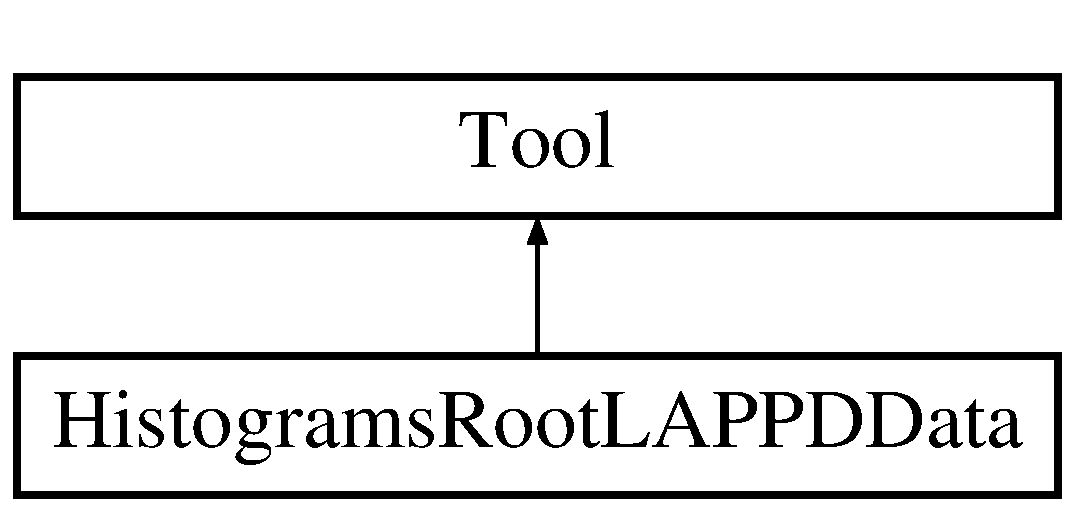
\includegraphics[height=2.000000cm]{classHistogramsRootLAPPDData}
\end{center}
\end{figure}
\subsection*{Public Member Functions}
\begin{DoxyCompactItemize}
\item 
\hypertarget{classHistogramsRootLAPPDData_ab87ee19ac23e1a888976464ec0e9b199}{bool {\bfseries Initialise} (std\-::string configfile, \hyperlink{classDataModel}{Data\-Model} \&data)}\label{classHistogramsRootLAPPDData_ab87ee19ac23e1a888976464ec0e9b199}

\item 
\hypertarget{classHistogramsRootLAPPDData_a81c098fc773fb9bb365beb47aefd67d7}{bool {\bfseries Execute} ()}\label{classHistogramsRootLAPPDData_a81c098fc773fb9bb365beb47aefd67d7}

\item 
\hypertarget{classHistogramsRootLAPPDData_abc484166b3afed20afc9a702c3a003da}{bool {\bfseries Finalise} ()}\label{classHistogramsRootLAPPDData_abc484166b3afed20afc9a702c3a003da}

\end{DoxyCompactItemize}


The documentation for this class was generated from the following file\-:\begin{DoxyCompactItemize}
\item 
User\-Tools/\-Histograms\-Root\-L\-A\-P\-P\-D\-Data/Histograms\-Root\-L\-A\-P\-P\-D\-Data.\-h\end{DoxyCompactItemize}

\hypertarget{classHit}{\section{Hit Class Reference}
\label{classHit}\index{Hit@{Hit}}
}
Inheritance diagram for Hit\-:\begin{figure}[H]
\begin{center}
\leavevmode
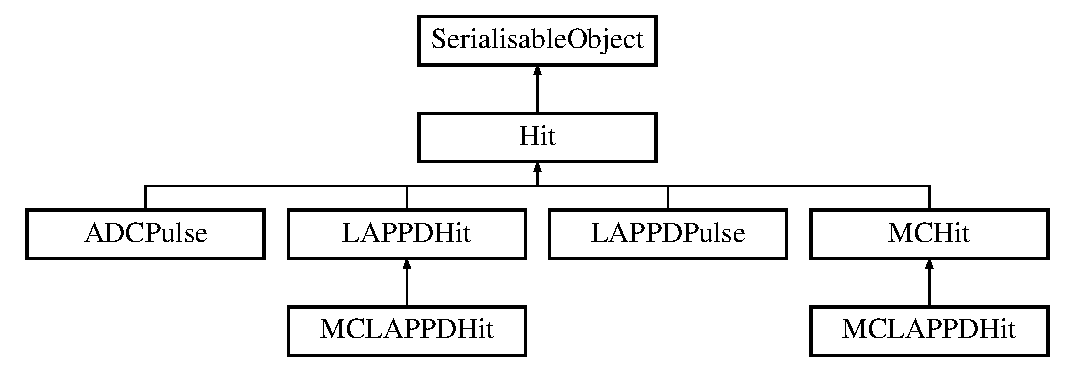
\includegraphics[height=4.000000cm]{classHit}
\end{center}
\end{figure}
\subsection*{Public Member Functions}
\begin{DoxyCompactItemize}
\item 
\hypertarget{classHit_a46c21425b896c5638598b4116de73740}{{\bfseries Hit} (int thetubeid, double thetime, double thecharge)}\label{classHit_a46c21425b896c5638598b4116de73740}

\item 
\hypertarget{classHit_ad4da9c11c8a203b65bd8b97b144a8133}{int {\bfseries Get\-Tube\-Id} () const }\label{classHit_ad4da9c11c8a203b65bd8b97b144a8133}

\item 
\hypertarget{classHit_aa67ab762ecf9eab3d41147667447c597}{double {\bfseries Get\-Time} () const }\label{classHit_aa67ab762ecf9eab3d41147667447c597}

\item 
\hypertarget{classHit_a77e2a2c8ed9449b38fc00e1d516d122a}{double {\bfseries Get\-Charge} () const }\label{classHit_a77e2a2c8ed9449b38fc00e1d516d122a}

\item 
\hypertarget{classHit_a2f1d81f94c9cfc35ba664b94fd719156}{void {\bfseries Set\-Tube\-Id} (int tubeid)}\label{classHit_a2f1d81f94c9cfc35ba664b94fd719156}

\item 
\hypertarget{classHit_af540ccdede0608cdd9ce6e754258b5e8}{void {\bfseries Set\-Time} (double tc)}\label{classHit_af540ccdede0608cdd9ce6e754258b5e8}

\item 
\hypertarget{classHit_aabbc33179a273289414263478835f2b9}{void {\bfseries Set\-Charge} (double chg)}\label{classHit_aabbc33179a273289414263478835f2b9}

\item 
\hypertarget{classHit_acebd1b0fb425a531faefed955f4c87e2}{bool {\bfseries Print} ()}\label{classHit_acebd1b0fb425a531faefed955f4c87e2}

\end{DoxyCompactItemize}
\subsection*{Protected Member Functions}
\begin{DoxyCompactItemize}
\item 
\hypertarget{classHit_af3bafb22cc7c2c224af22927c6ea2d07}{{\footnotesize template$<$class Archive $>$ }\\void {\bfseries serialize} (Archive \&ar, const unsigned int version)}\label{classHit_af3bafb22cc7c2c224af22927c6ea2d07}

\end{DoxyCompactItemize}
\subsection*{Protected Attributes}
\begin{DoxyCompactItemize}
\item 
\hypertarget{classHit_a442f7a2eebdfbc0e8c29194f4e26e40e}{int {\bfseries Tube\-Id}}\label{classHit_a442f7a2eebdfbc0e8c29194f4e26e40e}

\item 
\hypertarget{classHit_a8abba0e32e50c99ed70f38f660486e29}{double {\bfseries Time}}\label{classHit_a8abba0e32e50c99ed70f38f660486e29}

\item 
\hypertarget{classHit_a6460be8aae8df3d04ae3871d99bf0193}{double {\bfseries Charge}}\label{classHit_a6460be8aae8df3d04ae3871d99bf0193}

\end{DoxyCompactItemize}
\subsection*{Friends}
\begin{DoxyCompactItemize}
\item 
\hypertarget{classHit_ac98d07dd8f7b70e16ccb9a01abf56b9c}{class {\bfseries boost\-::serialization\-::access}}\label{classHit_ac98d07dd8f7b70e16ccb9a01abf56b9c}

\end{DoxyCompactItemize}


The documentation for this class was generated from the following file\-:\begin{DoxyCompactItemize}
\item 
Data\-Model/Hit.\-h\end{DoxyCompactItemize}

\hypertarget{classHitCleaner}{\section{Hit\-Cleaner Class Reference}
\label{classHitCleaner}\index{Hit\-Cleaner@{Hit\-Cleaner}}
}
Inheritance diagram for Hit\-Cleaner\-:\begin{figure}[H]
\begin{center}
\leavevmode
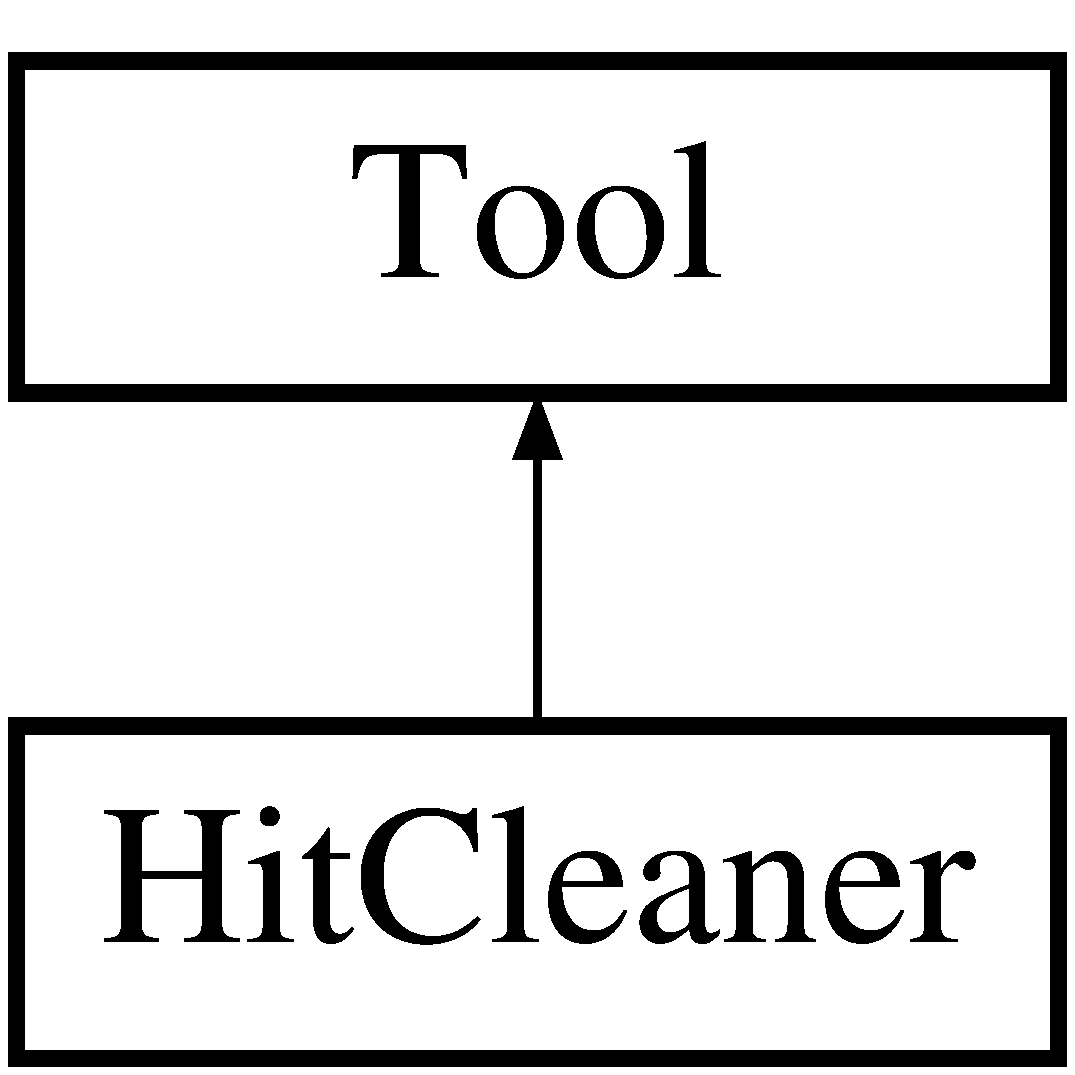
\includegraphics[height=2.000000cm]{classHitCleaner}
\end{center}
\end{figure}
\subsection*{Public Types}
\begin{DoxyCompactItemize}
\item 
enum {\bfseries E\-Filter\-Config} \{ \\*
{\bfseries k\-None} = 0, 
{\bfseries k\-Pulse\-Height} = 1, 
{\bfseries k\-Pulse\-Height\-And\-Neighbours} = 2, 
{\bfseries k\-Pulse\-Height\-And\-Clusters} = 3, 
\\*
{\bfseries k\-Pulse\-Height\-And\-Truth\-Info} = 3
 \}
\item 
\hypertarget{classHitCleaner_a417732ebe6c9a62f91a0648522cb5e01}{typedef enum \\*
Hit\-Cleaner\-::\-E\-Filter\-Config {\bfseries Filter\-Config\-\_\-t}}\label{classHitCleaner_a417732ebe6c9a62f91a0648522cb5e01}

\end{DoxyCompactItemize}
\subsection*{Public Member Functions}
\begin{DoxyCompactItemize}
\item 
bool \hyperlink{classHitCleaner_a35bd6ca1401c52439166e51c7e873ace}{Initialise} (std\-::string configfile, \hyperlink{classDataModel}{Data\-Model} \&data)
\item 
bool \hyperlink{classHitCleaner_adec5b94400dcbfc710590d7eb387041b}{Execute} ()
\item 
\hypertarget{classHitCleaner_a06d16e3d574ec685952c011d2309fa76}{bool {\bfseries Finalise} ()}\label{classHitCleaner_a06d16e3d574ec685952c011d2309fa76}

\item 
\hypertarget{classHitCleaner_a2d7f24be0dae3a9aa53771bc0bdb65c6}{void {\bfseries Print\-Parameters} ()}\label{classHitCleaner_a2d7f24be0dae3a9aa53771bc0bdb65c6}

\item 
\hypertarget{classHitCleaner_af75191aadcf2acffcc1c13549d062fc8}{void {\bfseries Set\-Config} (int config)}\label{classHitCleaner_af75191aadcf2acffcc1c13549d062fc8}

\item 
\hypertarget{classHitCleaner_acb667165fb7166a54b5401264c76cf60}{void {\bfseries Set\-Pmt\-Min\-Pulse\-Height} (double min)}\label{classHitCleaner_acb667165fb7166a54b5401264c76cf60}

\item 
\hypertarget{classHitCleaner_a48ecb1833030a1e53d76f852735b1146}{void {\bfseries Set\-Pmt\-Neighbour\-Radius} (double radius)}\label{classHitCleaner_a48ecb1833030a1e53d76f852735b1146}

\item 
\hypertarget{classHitCleaner_a05aaf25ef5464e2cc0cbb67a123a4683}{void {\bfseries Set\-Pmt\-Neighbour\-Digits} (int digits)}\label{classHitCleaner_a05aaf25ef5464e2cc0cbb67a123a4683}

\item 
\hypertarget{classHitCleaner_a374f2c25fd741ba89253c1df57c2f711}{void {\bfseries Set\-Pmt\-Cluster\-Radius} (double radius)}\label{classHitCleaner_a374f2c25fd741ba89253c1df57c2f711}

\item 
\hypertarget{classHitCleaner_a2034dc5fabc9bd6a7f06bfe9be9172f4}{void {\bfseries Set\-Pmt\-Time\-Window\-Neighbours} (double window\-N)}\label{classHitCleaner_a2034dc5fabc9bd6a7f06bfe9be9172f4}

\item 
\hypertarget{classHitCleaner_a5d427dd83732333d8918993e2c5a08d2}{void {\bfseries Set\-Pmt\-Time\-Window\-Clusters} (double window\-C)}\label{classHitCleaner_a5d427dd83732333d8918993e2c5a08d2}

\item 
\hypertarget{classHitCleaner_abe7877bee548ff2e72db4991ebe8d9b1}{void {\bfseries Set\-Lappd\-Min\-Pulse\-Height} (double min)}\label{classHitCleaner_abe7877bee548ff2e72db4991ebe8d9b1}

\item 
\hypertarget{classHitCleaner_a3deef1a55f3597115b7a1514c23ab2b4}{void {\bfseries Set\-Lappd\-Neighbour\-Radius} (double radius)}\label{classHitCleaner_a3deef1a55f3597115b7a1514c23ab2b4}

\item 
\hypertarget{classHitCleaner_af872da7d231440f4fa75b2dfe6be5fc8}{void {\bfseries Set\-Lappd\-Neighbour\-Digits} (int digits)}\label{classHitCleaner_af872da7d231440f4fa75b2dfe6be5fc8}

\item 
\hypertarget{classHitCleaner_aacf88b73ee3bb0bb4afa4648c64add65}{void {\bfseries Set\-Lappd\-Cluster\-Radius} (double radius)}\label{classHitCleaner_aacf88b73ee3bb0bb4afa4648c64add65}

\item 
\hypertarget{classHitCleaner_aaa0aca2da3c1a4670e9a4a1361e9b124}{void {\bfseries Set\-Lappd\-Time\-Window\-Neighbours} (double window\-N)}\label{classHitCleaner_aaa0aca2da3c1a4670e9a4a1361e9b124}

\item 
\hypertarget{classHitCleaner_a093989b06deb5743b6c4c81092e69ceb}{void {\bfseries Set\-Lappd\-Time\-Window\-Clusters} (double window\-C)}\label{classHitCleaner_a093989b06deb5743b6c4c81092e69ceb}

\item 
\hypertarget{classHitCleaner_a6f25436f395cb868857f7a4b5c418de2}{void {\bfseries Load\-Config\-File} (string configfilename)}\label{classHitCleaner_a6f25436f395cb868857f7a4b5c418de2}

\item 
\hypertarget{classHitCleaner_a1154c24324e11dc8d0d53bcd806d7113}{void {\bfseries Set\-Min\-Cluster\-Digits} (int digits)}\label{classHitCleaner_a1154c24324e11dc8d0d53bcd806d7113}

\item 
\hypertarget{classHitCleaner_ae47191a46b30d5345b1e1c422767f816}{std\-::vector$<$ \hyperlink{classRecoDigit}{Reco\-Digit} $\ast$ $>$ $\ast$ {\bfseries Run} (std\-::vector$<$ \hyperlink{classRecoDigit}{Reco\-Digit} $\ast$ $>$ $\ast$digitlist)}\label{classHitCleaner_ae47191a46b30d5345b1e1c422767f816}

\item 
\hypertarget{classHitCleaner_a3c85370ccb39e1615976fe4acb218fb5}{std\-::vector$<$ \hyperlink{classRecoDigit}{Reco\-Digit} $\ast$ $>$ $\ast$ {\bfseries Reset\-Digits} (std\-::vector$<$ \hyperlink{classRecoDigit}{Reco\-Digit} $\ast$ $>$ $\ast$digitlist)}\label{classHitCleaner_a3c85370ccb39e1615976fe4acb218fb5}

\item 
\hypertarget{classHitCleaner_a16028ae7a55a4cdcfdb116af893d2542}{std\-::vector$<$ \hyperlink{classRecoDigit}{Reco\-Digit} $\ast$ $>$ $\ast$ {\bfseries Filter\-Digits} (std\-::vector$<$ \hyperlink{classRecoDigit}{Reco\-Digit} $\ast$ $>$ $\ast$digitlist)}\label{classHitCleaner_a16028ae7a55a4cdcfdb116af893d2542}

\item 
\hypertarget{classHitCleaner_a7e6188a785adddfcaa3dbe63de387e95}{std\-::vector$<$ \hyperlink{classRecoDigit}{Reco\-Digit} $\ast$ $>$ $\ast$ {\bfseries Filter\-All} (std\-::vector$<$ \hyperlink{classRecoDigit}{Reco\-Digit} $\ast$ $>$ $\ast$digitlist)}\label{classHitCleaner_a7e6188a785adddfcaa3dbe63de387e95}

\item 
\hypertarget{classHitCleaner_a537c7f9b371c0dc52df86046f8a90336}{std\-::vector$<$ \hyperlink{classRecoDigit}{Reco\-Digit} $\ast$ $>$ $\ast$ {\bfseries Filter\-By\-Pulse\-Height} (std\-::vector$<$ \hyperlink{classRecoDigit}{Reco\-Digit} $\ast$ $>$ $\ast$digitlist)}\label{classHitCleaner_a537c7f9b371c0dc52df86046f8a90336}

\item 
\hypertarget{classHitCleaner_ad574e2c8d1718971cbfce2a284731daa}{std\-::vector$<$ \hyperlink{classRecoDigit}{Reco\-Digit} $\ast$ $>$ $\ast$ {\bfseries Filter\-By\-Neighbours} (std\-::vector$<$ \hyperlink{classRecoDigit}{Reco\-Digit} $\ast$ $>$ $\ast$digitlist)}\label{classHitCleaner_ad574e2c8d1718971cbfce2a284731daa}

\item 
\hypertarget{classHitCleaner_a32e29edc8c7564e423186efacbea07c5}{std\-::vector$<$ \hyperlink{classRecoDigit}{Reco\-Digit} $\ast$ $>$ $\ast$ {\bfseries Filter\-By\-Clusters} (std\-::vector$<$ \hyperlink{classRecoDigit}{Reco\-Digit} $\ast$ $>$ $\ast$digitlist)}\label{classHitCleaner_a32e29edc8c7564e423186efacbea07c5}

\item 
\hypertarget{classHitCleaner_ad2c117045b0a63c700b0f2a94f3fa0b2}{std\-::vector$<$ \hyperlink{classRecoDigit}{Reco\-Digit} $\ast$ $>$ $\ast$ {\bfseries Filter\-By\-Truth\-Info} (std\-::vector$<$ \hyperlink{classRecoDigit}{Reco\-Digit} $\ast$ $>$ $\ast$digitlist)}\label{classHitCleaner_ad2c117045b0a63c700b0f2a94f3fa0b2}

\item 
\hypertarget{classHitCleaner_a0e516802fcbaad1e3e61978911991949}{std\-::vector$<$ \hyperlink{classRecoCluster}{Reco\-Cluster} $\ast$ $>$ $\ast$ {\bfseries Reco\-Clusters} (std\-::vector$<$ \hyperlink{classRecoDigit}{Reco\-Digit} $\ast$ $>$ $\ast$digitlist)}\label{classHitCleaner_a0e516802fcbaad1e3e61978911991949}

\end{DoxyCompactItemize}
\subsection*{Static Public Member Functions}
\begin{DoxyCompactItemize}
\item 
\hypertarget{classHitCleaner_a4ac1bde4eec18c427ed249409a6d5d3a}{static \hyperlink{classHitCleaner}{Hit\-Cleaner} $\ast$ {\bfseries Instance} ()}\label{classHitCleaner_a4ac1bde4eec18c427ed249409a6d5d3a}

\item 
\hypertarget{classHitCleaner_afdf345b322cbef82deb9f35eaddb02d1}{static void {\bfseries Config} (int config)}\label{classHitCleaner_afdf345b322cbef82deb9f35eaddb02d1}

\item 
\hypertarget{classHitCleaner_a94987b09a59d9781277f76eee63994a1}{static void {\bfseries Pmt\-Min\-Pulse\-Height} (double min)}\label{classHitCleaner_a94987b09a59d9781277f76eee63994a1}

\item 
\hypertarget{classHitCleaner_af6d017ac189b0eb6abf064756e78f5ac}{static void {\bfseries Pmt\-Neighbour\-Radius} (double radius)}\label{classHitCleaner_af6d017ac189b0eb6abf064756e78f5ac}

\item 
\hypertarget{classHitCleaner_a43b5a1ac75e62334a8e9ff539a9b34df}{static void {\bfseries Pmt\-Neighbour\-Digits} (int digits)}\label{classHitCleaner_a43b5a1ac75e62334a8e9ff539a9b34df}

\item 
\hypertarget{classHitCleaner_a71881188d23e57c9afb0c8179ff9c5e3}{static void {\bfseries Pmt\-Cluster\-Radius} (double radius)}\label{classHitCleaner_a71881188d23e57c9afb0c8179ff9c5e3}

\item 
\hypertarget{classHitCleaner_a8074ae3702ee872e8c8b4504f3bf3987}{static void {\bfseries Min\-Cluster\-Digits} (int digits)}\label{classHitCleaner_a8074ae3702ee872e8c8b4504f3bf3987}

\item 
\hypertarget{classHitCleaner_a2efa2634319c4ff56e51ba28415146a9}{static void {\bfseries Pmt\-Time\-Window\-N} (double window\-N)}\label{classHitCleaner_a2efa2634319c4ff56e51ba28415146a9}

\item 
\hypertarget{classHitCleaner_a1962dfdb70798529f8f560c1b6f233fc}{static void {\bfseries Pmt\-Time\-Window\-C} (double window\-C)}\label{classHitCleaner_a1962dfdb70798529f8f560c1b6f233fc}

\end{DoxyCompactItemize}


\subsection{Member Function Documentation}
\hypertarget{classHitCleaner_adec5b94400dcbfc710590d7eb387041b}{\index{Hit\-Cleaner@{Hit\-Cleaner}!Execute@{Execute}}
\index{Execute@{Execute}!HitCleaner@{Hit\-Cleaner}}
\subsubsection[{Execute}]{\setlength{\rightskip}{0pt plus 5cm}bool Hit\-Cleaner\-::\-Execute (
\begin{DoxyParamCaption}
{}
\end{DoxyParamCaption}
)}}\label{classHitCleaner_adec5b94400dcbfc710590d7eb387041b}
see if \char`\"{}\-Reco\-Event\char`\"{} exists

\begin{quotation}
Get digits from \char`\"{}\-Reco\-Event\char`\"{} \end{quotation}
\hypertarget{classHitCleaner_a35bd6ca1401c52439166e51c7e873ace}{\index{Hit\-Cleaner@{Hit\-Cleaner}!Initialise@{Initialise}}
\index{Initialise@{Initialise}!HitCleaner@{Hit\-Cleaner}}
\subsubsection[{Initialise}]{\setlength{\rightskip}{0pt plus 5cm}bool Hit\-Cleaner\-::\-Initialise (
\begin{DoxyParamCaption}
\item[{std\-::string}]{configfile, }
\item[{{\bf Data\-Model} \&}]{data}
\end{DoxyParamCaption}
)}}\label{classHitCleaner_a35bd6ca1401c52439166e51c7e873ace}
Get the Tool configuration variables 

The documentation for this class was generated from the following files\-:\begin{DoxyCompactItemize}
\item 
User\-Tools/\-Hit\-Cleaner/Hit\-Cleaner.\-h\item 
User\-Tools/\-Hit\-Cleaner/Hit\-Cleaner.\-cpp\end{DoxyCompactItemize}

\hypertarget{classHitResiduals}{
\section{HitResiduals Class Reference}
\label{classHitResiduals}\index{HitResiduals@{HitResiduals}}
}
\subsection*{Public Member Functions}
\begin{DoxyCompactItemize}
\item 
\hypertarget{classHitResiduals_ac37e7a71c2fece45c304383ace201de8}{
bool {\bfseries Initialise} (std::string configfile, \hyperlink{classDataModel}{DataModel} \&data)}
\label{classHitResiduals_ac37e7a71c2fece45c304383ace201de8}

\item 
\hypertarget{classHitResiduals_a6715e864b1c07e812178cc0d3b245339}{
bool {\bfseries Execute} ()}
\label{classHitResiduals_a6715e864b1c07e812178cc0d3b245339}

\item 
\hypertarget{classHitResiduals_a00c3b75308417bfd468cbb786104c26f}{
bool {\bfseries Finalise} ()}
\label{classHitResiduals_a00c3b75308417bfd468cbb786104c26f}

\end{DoxyCompactItemize}


The documentation for this class was generated from the following files:\begin{DoxyCompactItemize}
\item 
UserTools/HitResiduals/HitResiduals.h\item 
UserTools/HitResiduals/HitResiduals.cpp\end{DoxyCompactItemize}

\hypertarget{classIFBeamDBInterface}{
\section{IFBeamDBInterface Class Reference}
\label{classIFBeamDBInterface}\index{IFBeamDBInterface@{IFBeamDBInterface}}
}


Singleton used to interact with the Intensity Frontier beam database at Fermilab.  


{\ttfamily \#include $<$IFBeamDBInterface.h$>$}\subsection*{Public Member Functions}
\begin{DoxyCompactItemize}
\item 
\hypertarget{classIFBeamDBInterface_ac6e95cfed4db9c455289234f26a2f1c1}{
\hyperlink{classIFBeamDBInterface_ac6e95cfed4db9c455289234f26a2f1c1}{$\sim$IFBeamDBInterface} ()}
\label{classIFBeamDBInterface_ac6e95cfed4db9c455289234f26a2f1c1}

\begin{DoxyCompactList}\small\item\em Clean up libcurl stuff as the \hyperlink{classIFBeamDBInterface}{IFBeamDBInterface} object is destroyed. \item\end{DoxyCompactList}\item 
\hypertarget{classIFBeamDBInterface_a5a3bc058c6b8ca2e3d13b85ca1f42e2d}{
\hyperlink{classIFBeamDBInterface_a5a3bc058c6b8ca2e3d13b85ca1f42e2d}{IFBeamDBInterface} (const \hyperlink{classIFBeamDBInterface}{IFBeamDBInterface} \&)}
\label{classIFBeamDBInterface_a5a3bc058c6b8ca2e3d13b85ca1f42e2d}

\begin{DoxyCompactList}\small\item\em Deleted copy constructor. \item\end{DoxyCompactList}\item 
\hypertarget{classIFBeamDBInterface_a25624ce40601f7ee32b039c34466d5cc}{
\hyperlink{classIFBeamDBInterface_a25624ce40601f7ee32b039c34466d5cc}{IFBeamDBInterface} (\hyperlink{classIFBeamDBInterface}{IFBeamDBInterface} \&\&)}
\label{classIFBeamDBInterface_a25624ce40601f7ee32b039c34466d5cc}

\begin{DoxyCompactList}\small\item\em Deleted move constructor. \item\end{DoxyCompactList}\item 
\hypertarget{classIFBeamDBInterface_a9550adf51f7c043e9ba628e920202ec2}{
\hyperlink{classIFBeamDBInterface}{IFBeamDBInterface} \& \hyperlink{classIFBeamDBInterface_a9550adf51f7c043e9ba628e920202ec2}{operator=} (const \hyperlink{classIFBeamDBInterface}{IFBeamDBInterface} \&)}
\label{classIFBeamDBInterface_a9550adf51f7c043e9ba628e920202ec2}

\begin{DoxyCompactList}\small\item\em Deleted copy assignment operator. \item\end{DoxyCompactList}\item 
\hypertarget{classIFBeamDBInterface_a66a70c1666620601852ceec5038c3c62}{
\hyperlink{classIFBeamDBInterface}{IFBeamDBInterface} \& \hyperlink{classIFBeamDBInterface_a66a70c1666620601852ceec5038c3c62}{operator=} (\hyperlink{classIFBeamDBInterface}{IFBeamDBInterface} \&\&)}
\label{classIFBeamDBInterface_a66a70c1666620601852ceec5038c3c62}

\begin{DoxyCompactList}\small\item\em Deleted move assignment operator. \item\end{DoxyCompactList}\item 
std::map$<$ std::string, std::map$<$ uint64\_\-t, \hyperlink{structBeamDataPoint}{BeamDataPoint} $>$ $>$ \hyperlink{classIFBeamDBInterface_a7b0e4c42767791f1904540b63772a74d}{QueryBeamDB} (uint64\_\-t t0, uint64\_\-t t1) const 
\begin{DoxyCompactList}\small\item\em Get information about the Booster Neutrino Beam (BNB) state from the database for the time interval \mbox{[}t0, t1\mbox{]}. \item\end{DoxyCompactList}\item 
int \hyperlink{classIFBeamDBInterface_a034ef023cb78989270a4ec2d54a5aa4f}{QueryBeamDB} (uint64\_\-t t0, uint64\_\-t t1, std::string \&response\_\-string) const 
\begin{DoxyCompactList}\small\item\em Get information about the BNB state from the database for the time interval \mbox{[}t0, t1\mbox{]}. \item\end{DoxyCompactList}\item 
\hyperlink{classBeamStatus}{BeamStatus} \hyperlink{classIFBeamDBInterface_add525c53cbf0b85c3cd0d39a5b9b0fdd}{GetBeamStatus} (uint64\_\-t time) const 
\begin{DoxyCompactList}\small\item\em Get information about the BNB state from the database as close as possible to a given time. \item\end{DoxyCompactList}\end{DoxyCompactItemize}
\subsection*{Static Public Member Functions}
\begin{DoxyCompactItemize}
\item 
\hypertarget{classIFBeamDBInterface_a677ed1a3b7dbfc70ffb0688078ae5fb0}{
static const \hyperlink{classIFBeamDBInterface}{IFBeamDBInterface} \& \hyperlink{classIFBeamDBInterface_a677ed1a3b7dbfc70ffb0688078ae5fb0}{Instance} ()}
\label{classIFBeamDBInterface_a677ed1a3b7dbfc70ffb0688078ae5fb0}

\begin{DoxyCompactList}\small\item\em Get a const reference to the singleton instance of the \hyperlink{classIFBeamDBInterface}{IFBeamDBInterface}. \item\end{DoxyCompactList}\end{DoxyCompactItemize}
\subsection*{Protected Member Functions}
\begin{DoxyCompactItemize}
\item 
\hypertarget{classIFBeamDBInterface_af5275e528b9b43d4c5dacd0a8a3ca62b}{
\hyperlink{classIFBeamDBInterface_af5275e528b9b43d4c5dacd0a8a3ca62b}{IFBeamDBInterface} ()}
\label{classIFBeamDBInterface_af5275e528b9b43d4c5dacd0a8a3ca62b}

\begin{DoxyCompactList}\small\item\em Create the singleton \hyperlink{classIFBeamDBInterface}{IFBeamDBInterface} object. \item\end{DoxyCompactList}\item 
\hypertarget{classIFBeamDBInterface_a950bec54fb41eaf48471a8a1eab8ab71}{
std::map$<$ std::string, std::map$<$ uint64\_\-t, \hyperlink{structBeamDataPoint}{BeamDataPoint} $>$ $>$ {\bfseries ParseDBResponse} (const std::string \&response) const }
\label{classIFBeamDBInterface_a950bec54fb41eaf48471a8a1eab8ab71}

\item 
\hypertarget{classIFBeamDBInterface_a2d7b151e8b21fe5f7d255d442d37e321}{
void {\bfseries PostprocessParsedResponse} (std::map$<$ std::string, std::map$<$ uint64\_\-t, \hyperlink{structBeamDataPoint}{BeamDataPoint} $>$ $>$ \&parsed\_\-response) const }
\label{classIFBeamDBInterface_a2d7b151e8b21fe5f7d255d442d37e321}

\end{DoxyCompactItemize}
\subsection*{Protected Attributes}
\begin{DoxyCompactItemize}
\item 
\hypertarget{classIFBeamDBInterface_a7dea07c539e0f0ca765f02d198345d2d}{
CURL $\ast$ \hyperlink{classIFBeamDBInterface_a7dea07c539e0f0ca765f02d198345d2d}{fCurl} = nullptr}
\label{classIFBeamDBInterface_a7dea07c539e0f0ca765f02d198345d2d}

\begin{DoxyCompactList}\small\item\em Pointer used to interact with libcurl. \item\end{DoxyCompactList}\end{DoxyCompactItemize}


\subsection{Detailed Description}
Singleton used to interact with the Intensity Frontier beam database at Fermilab. 

\subsection{Member Function Documentation}
\hypertarget{classIFBeamDBInterface_add525c53cbf0b85c3cd0d39a5b9b0fdd}{
\index{IFBeamDBInterface@{IFBeamDBInterface}!GetBeamStatus@{GetBeamStatus}}
\index{GetBeamStatus@{GetBeamStatus}!IFBeamDBInterface@{IFBeamDBInterface}}
\subsubsection[{GetBeamStatus}]{\setlength{\rightskip}{0pt plus 5cm}{\bf BeamStatus} IFBeamDBInterface::GetBeamStatus (uint64\_\-t {\em time}) const}}
\label{classIFBeamDBInterface_add525c53cbf0b85c3cd0d39a5b9b0fdd}


Get information about the BNB state from the database as close as possible to a given time. 
\begin{DoxyParams}{Parameters}
\item[{\em time}]Timestamp (milliseconds since the Unix epoch) to use when searching the database \end{DoxyParams}
\hypertarget{classIFBeamDBInterface_a034ef023cb78989270a4ec2d54a5aa4f}{
\index{IFBeamDBInterface@{IFBeamDBInterface}!QueryBeamDB@{QueryBeamDB}}
\index{QueryBeamDB@{QueryBeamDB}!IFBeamDBInterface@{IFBeamDBInterface}}
\subsubsection[{QueryBeamDB}]{\setlength{\rightskip}{0pt plus 5cm}int IFBeamDBInterface::QueryBeamDB (uint64\_\-t {\em t0}, \/  uint64\_\-t {\em t1}, \/  std::string \& {\em response\_\-string}) const}}
\label{classIFBeamDBInterface_a034ef023cb78989270a4ec2d54a5aa4f}


Get information about the BNB state from the database for the time interval \mbox{[}t0, t1\mbox{]}. 
\begin{DoxyParams}{Parameters}
\item[{\em t0}]Starting timestamp (milliseconds since the Unix epoch) \item[{\em t1}]Starting timestamp (milliseconds since the Unix epoch) \item[\mbox{$\rightarrow$} {\em response\_\-string}]A string that will be loaded with the csv-\/format data from the database \end{DoxyParams}
\begin{DoxyReturn}{Returns}
The libcurl integer return code for the query (zero if everything worked ok, or nonzero if an error occurred) 
\end{DoxyReturn}
\hypertarget{classIFBeamDBInterface_a7b0e4c42767791f1904540b63772a74d}{
\index{IFBeamDBInterface@{IFBeamDBInterface}!QueryBeamDB@{QueryBeamDB}}
\index{QueryBeamDB@{QueryBeamDB}!IFBeamDBInterface@{IFBeamDBInterface}}
\subsubsection[{QueryBeamDB}]{\setlength{\rightskip}{0pt plus 5cm}std::map$<$ std::string, std::map$<$ uint64\_\-t, {\bf BeamDataPoint} $>$ $>$ IFBeamDBInterface::QueryBeamDB (uint64\_\-t {\em t0}, \/  uint64\_\-t {\em t1}) const}}
\label{classIFBeamDBInterface_a7b0e4c42767791f1904540b63772a74d}


Get information about the Booster Neutrino Beam (BNB) state from the database for the time interval \mbox{[}t0, t1\mbox{]}. 
\begin{DoxyParams}{Parameters}
\item[{\em t0}]Starting timestamp (milliseconds since the Unix epoch) \item[{\em t1}]Starting timestamp (milliseconds since the Unix epoch) \end{DoxyParams}
\begin{DoxyReturn}{Returns}
A nested map containing the parsed data. Keys of the outer map are device names, values are inner maps. Keys of the inner map are timestamps (milliseconds since the Unix epoch), values are \hyperlink{structBeamDataPoint}{BeamDataPoint} structs that hold a numerical value and a unit string. 
\end{DoxyReturn}
\begin{DoxyNote}{Note}
An easy way to get the current milliseconds since the Unix epoch is to use the terminal utility date like this: \begin{DoxyVerb}date +%s%3N
    /// \end{DoxyVerb}
 I found this handy trick here: \href{http://unix.stackexchange.com/a/123764}{\tt http://unix.stackexchange.com/a/123764} 
\end{DoxyNote}


The documentation for this class was generated from the following files:\begin{DoxyCompactItemize}
\item 
UserTools/BeamFetcher/IFBeamDBInterface.h\item 
UserTools/BeamFetcher/IFBeamDBInterface.cpp\end{DoxyCompactItemize}

\hypertarget{classLAPPD}{
\section{LAPPD Class Reference}
\label{classLAPPD}\index{LAPPD@{LAPPD}}
}
\subsection*{Public Member Functions}
\begin{DoxyCompactItemize}
\item 
\hypertarget{classLAPPD_a6ef9e3c05e38b61c75cd12822ab5ce98}{
bool {\bfseries Print} ()}
\label{classLAPPD_a6ef9e3c05e38b61c75cd12822ab5ce98}

\end{DoxyCompactItemize}
\subsection*{Public Attributes}
\begin{DoxyCompactItemize}
\item 
\hypertarget{classLAPPD_a1b6bdd53a3523932fe22ad3b5471c91b}{
std::vector$<$ double $>$ {\bfseries waveform}}
\label{classLAPPD_a1b6bdd53a3523932fe22ad3b5471c91b}

\end{DoxyCompactItemize}
\subsection*{Friends}
\begin{DoxyCompactItemize}
\item 
\hypertarget{classLAPPD_ac98d07dd8f7b70e16ccb9a01abf56b9c}{
class {\bfseries boost::serialization::access}}
\label{classLAPPD_ac98d07dd8f7b70e16ccb9a01abf56b9c}

\end{DoxyCompactItemize}


The documentation for this class was generated from the following file:\begin{DoxyCompactItemize}
\item 
DataModel/LAPPD.h\end{DoxyCompactItemize}

\hypertarget{classLAPPDAnalysis}{
\section{LAPPDAnalysis Class Reference}
\label{classLAPPDAnalysis}\index{LAPPDAnalysis@{LAPPDAnalysis}}
}
\subsection*{Public Member Functions}
\begin{DoxyCompactItemize}
\item 
\hypertarget{classLAPPDAnalysis_a3777b97151a13ebc1be6054b057b7354}{
bool {\bfseries Initialise} (std::string configfile, \hyperlink{classDataModel}{DataModel} \&data)}
\label{classLAPPDAnalysis_a3777b97151a13ebc1be6054b057b7354}

\item 
\hypertarget{classLAPPDAnalysis_a0bda0e3aa26131d460e8f11ac2d2d50d}{
bool {\bfseries Execute} ()}
\label{classLAPPDAnalysis_a0bda0e3aa26131d460e8f11ac2d2d50d}

\item 
\hypertarget{classLAPPDAnalysis_acbda60c00d2f2bceca57ff9f9098e7a7}{
bool {\bfseries Finalise} ()}
\label{classLAPPDAnalysis_acbda60c00d2f2bceca57ff9f9098e7a7}

\end{DoxyCompactItemize}


The documentation for this class was generated from the following files:\begin{DoxyCompactItemize}
\item 
UserTools/LAPPDAnalysis/LAPPDAnalysis.h\item 
UserTools/LAPPDAnalysis/LAPPDAnalysis.cpp\end{DoxyCompactItemize}

\hypertarget{classLAPPDBaselineSubtract}{
\section{LAPPDBaselineSubtract Class Reference}
\label{classLAPPDBaselineSubtract}\index{LAPPDBaselineSubtract@{LAPPDBaselineSubtract}}
}
\subsection*{Public Member Functions}
\begin{DoxyCompactItemize}
\item 
\hypertarget{classLAPPDBaselineSubtract_a9173849be0de9676949ce9e3094c0c73}{
bool {\bfseries Initialise} (std::string configfile, \hyperlink{classDataModel}{DataModel} \&data)}
\label{classLAPPDBaselineSubtract_a9173849be0de9676949ce9e3094c0c73}

\item 
\hypertarget{classLAPPDBaselineSubtract_ae2ea261ef543fa9b924a1504a250b744}{
bool {\bfseries Execute} ()}
\label{classLAPPDBaselineSubtract_ae2ea261ef543fa9b924a1504a250b744}

\item 
\hypertarget{classLAPPDBaselineSubtract_a784d6efcf77a1cb4ad27b571f3a55d8d}{
bool {\bfseries Finalise} ()}
\label{classLAPPDBaselineSubtract_a784d6efcf77a1cb4ad27b571f3a55d8d}

\end{DoxyCompactItemize}


The documentation for this class was generated from the following files:\begin{DoxyCompactItemize}
\item 
UserTools/LAPPDBaselineSubtract/LAPPDBaselineSubtract.h\item 
UserTools/LAPPDBaselineSubtract/LAPPDBaselineSubtract.cpp\end{DoxyCompactItemize}

\hypertarget{classLAPPDcfd}{
\section{LAPPDcfd Class Reference}
\label{classLAPPDcfd}\index{LAPPDcfd@{LAPPDcfd}}
}
\subsection*{Public Member Functions}
\begin{DoxyCompactItemize}
\item 
\hypertarget{classLAPPDcfd_a712d671041c6dd069c060ad9eee43b5f}{
bool {\bfseries Initialise} (std::string configfile, \hyperlink{classDataModel}{DataModel} \&data)}
\label{classLAPPDcfd_a712d671041c6dd069c060ad9eee43b5f}

\item 
\hypertarget{classLAPPDcfd_a7776cd36991d9ccd6ed510c58b83f765}{
bool {\bfseries Execute} ()}
\label{classLAPPDcfd_a7776cd36991d9ccd6ed510c58b83f765}

\item 
\hypertarget{classLAPPDcfd_a9506c223f4626d40539efd132fc21acc}{
bool {\bfseries Finalise} ()}
\label{classLAPPDcfd_a9506c223f4626d40539efd132fc21acc}

\item 
\hypertarget{classLAPPDcfd_a81ca5d4bda97c4e0aeb8440af918a799}{
double {\bfseries CFD\_\-Discriminator1} (std::vector$<$ double $>$ $\ast$trace, \hyperlink{classLAPPDPulse}{LAPPDPulse} pulse)}
\label{classLAPPDcfd_a81ca5d4bda97c4e0aeb8440af918a799}

\item 
\hypertarget{classLAPPDcfd_a6473bfb16d498aa3ac23b566fe2a4d89}{
double {\bfseries CFD\_\-Discriminator2} (std::vector$<$ double $>$ $\ast$trace, \hyperlink{classLAPPDPulse}{LAPPDPulse} pulse)}
\label{classLAPPDcfd_a6473bfb16d498aa3ac23b566fe2a4d89}

\end{DoxyCompactItemize}


The documentation for this class was generated from the following files:\begin{DoxyCompactItemize}
\item 
UserTools/LAPPDcfd/LAPPDcfd.h\item 
UserTools/LAPPDcfd/LAPPDcfd.cpp\end{DoxyCompactItemize}

\hypertarget{classLAPPDFilter}{
\section{LAPPDFilter Class Reference}
\label{classLAPPDFilter}\index{LAPPDFilter@{LAPPDFilter}}
}
\subsection*{Public Member Functions}
\begin{DoxyCompactItemize}
\item 
\hypertarget{classLAPPDFilter_a43acf78f4842009ea98dbea3cc8dcaee}{
bool {\bfseries Initialise} (std::string configfile, \hyperlink{classDataModel}{DataModel} \&data)}
\label{classLAPPDFilter_a43acf78f4842009ea98dbea3cc8dcaee}

\item 
\hypertarget{classLAPPDFilter_a1aea3cb930e491d79248dd24ecd703c8}{
bool {\bfseries Execute} ()}
\label{classLAPPDFilter_a1aea3cb930e491d79248dd24ecd703c8}

\item 
\hypertarget{classLAPPDFilter_a5d6a46a70be7f2320fe3fe401d3efeba}{
bool {\bfseries Finalise} ()}
\label{classLAPPDFilter_a5d6a46a70be7f2320fe3fe401d3efeba}

\end{DoxyCompactItemize}


The documentation for this class was generated from the following files:\begin{DoxyCompactItemize}
\item 
UserTools/LAPPDFilter/LAPPDFilter.h\item 
UserTools/LAPPDFilter/LAPPDFilter.cpp\end{DoxyCompactItemize}

\hypertarget{classLAPPDFindPeak}{\section{L\-A\-P\-P\-D\-Find\-Peak Class Reference}
\label{classLAPPDFindPeak}\index{L\-A\-P\-P\-D\-Find\-Peak@{L\-A\-P\-P\-D\-Find\-Peak}}
}
Inheritance diagram for L\-A\-P\-P\-D\-Find\-Peak\-:\begin{figure}[H]
\begin{center}
\leavevmode
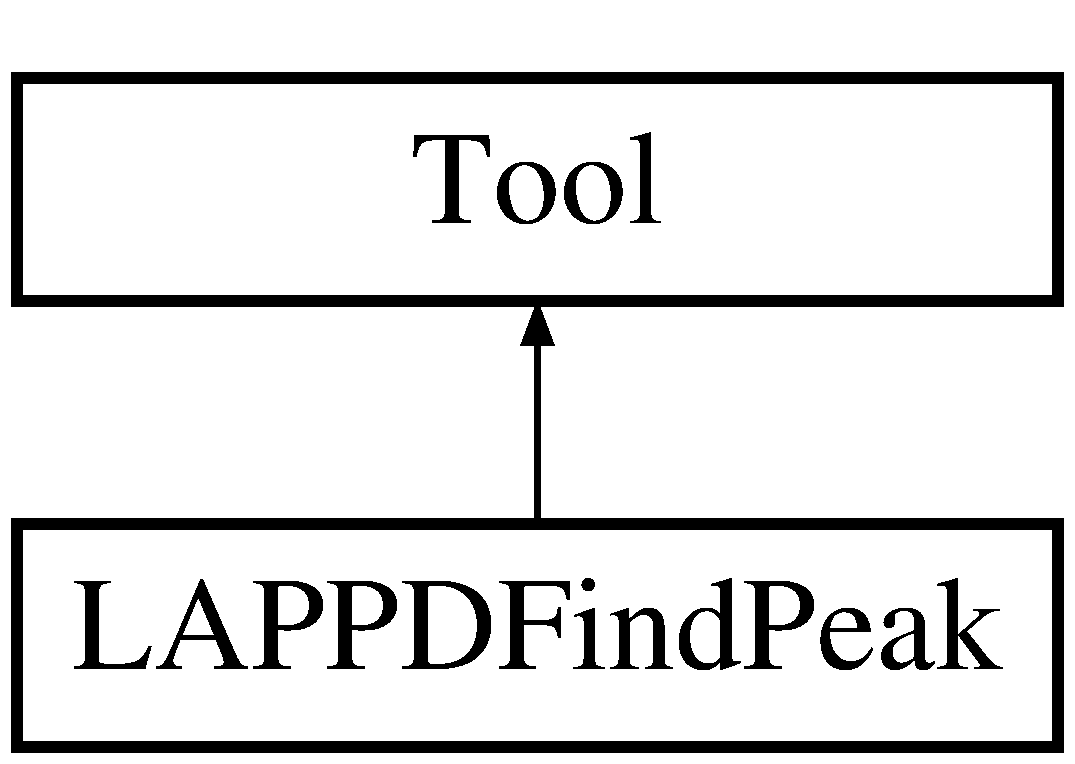
\includegraphics[height=2.000000cm]{classLAPPDFindPeak}
\end{center}
\end{figure}
\subsection*{Public Member Functions}
\begin{DoxyCompactItemize}
\item 
\hypertarget{classLAPPDFindPeak_aac02ab0efc1d6f2ac438a50a6dd48b51}{bool {\bfseries Initialise} (std\-::string configfile, \hyperlink{classDataModel}{Data\-Model} \&data)}\label{classLAPPDFindPeak_aac02ab0efc1d6f2ac438a50a6dd48b51}

\item 
\hypertarget{classLAPPDFindPeak_aeb178a0e7f0182bcec6aec80de1fd80c}{bool {\bfseries Execute} ()}\label{classLAPPDFindPeak_aeb178a0e7f0182bcec6aec80de1fd80c}

\item 
\hypertarget{classLAPPDFindPeak_a1c31ce2e8918e04c9e051a8c7eef304c}{bool {\bfseries Finalise} ()}\label{classLAPPDFindPeak_a1c31ce2e8918e04c9e051a8c7eef304c}

\item 
\hypertarget{classLAPPDFindPeak_aec4e759a18ce8bd5eda0ed4c1460ea4d}{std\-::vector$<$ \hyperlink{classLAPPDPulse}{L\-A\-P\-P\-D\-Pulse} $>$ {\bfseries Find\-Pulses\-\_\-\-T\-O\-T} (std\-::vector$<$ double $>$ $\ast$the\-Wav)}\label{classLAPPDFindPeak_aec4e759a18ce8bd5eda0ed4c1460ea4d}

\item 
\hypertarget{classLAPPDFindPeak_a705d781b236ed980dc6f6d4a297a5761}{std\-::vector$<$ \hyperlink{classLAPPDPulse}{L\-A\-P\-P\-D\-Pulse} $>$ {\bfseries Find\-Pulses\-\_\-\-Thresh} (std\-::vector$<$ double $>$ $\ast$the\-Wav)}\label{classLAPPDFindPeak_a705d781b236ed980dc6f6d4a297a5761}

\end{DoxyCompactItemize}
\subsection*{Public Attributes}
\begin{DoxyCompactItemize}
\item 
\hypertarget{classLAPPDFindPeak_a65501ad571e2fa607ba84239eab718af}{string {\bfseries Peak\-Input\-Wav\-Label}}\label{classLAPPDFindPeak_a65501ad571e2fa607ba84239eab718af}

\end{DoxyCompactItemize}


The documentation for this class was generated from the following files\-:\begin{DoxyCompactItemize}
\item 
User\-Tools/\-L\-A\-P\-P\-D\-Find\-Peak/L\-A\-P\-P\-D\-Find\-Peak.\-h\item 
User\-Tools/\-L\-A\-P\-P\-D\-Find\-Peak/L\-A\-P\-P\-D\-Find\-Peak.\-cpp\end{DoxyCompactItemize}

\hypertarget{classLAPPDHit}{\section{L\-A\-P\-P\-D\-Hit Class Reference}
\label{classLAPPDHit}\index{L\-A\-P\-P\-D\-Hit@{L\-A\-P\-P\-D\-Hit}}
}
Inheritance diagram for L\-A\-P\-P\-D\-Hit\-:\begin{figure}[H]
\begin{center}
\leavevmode
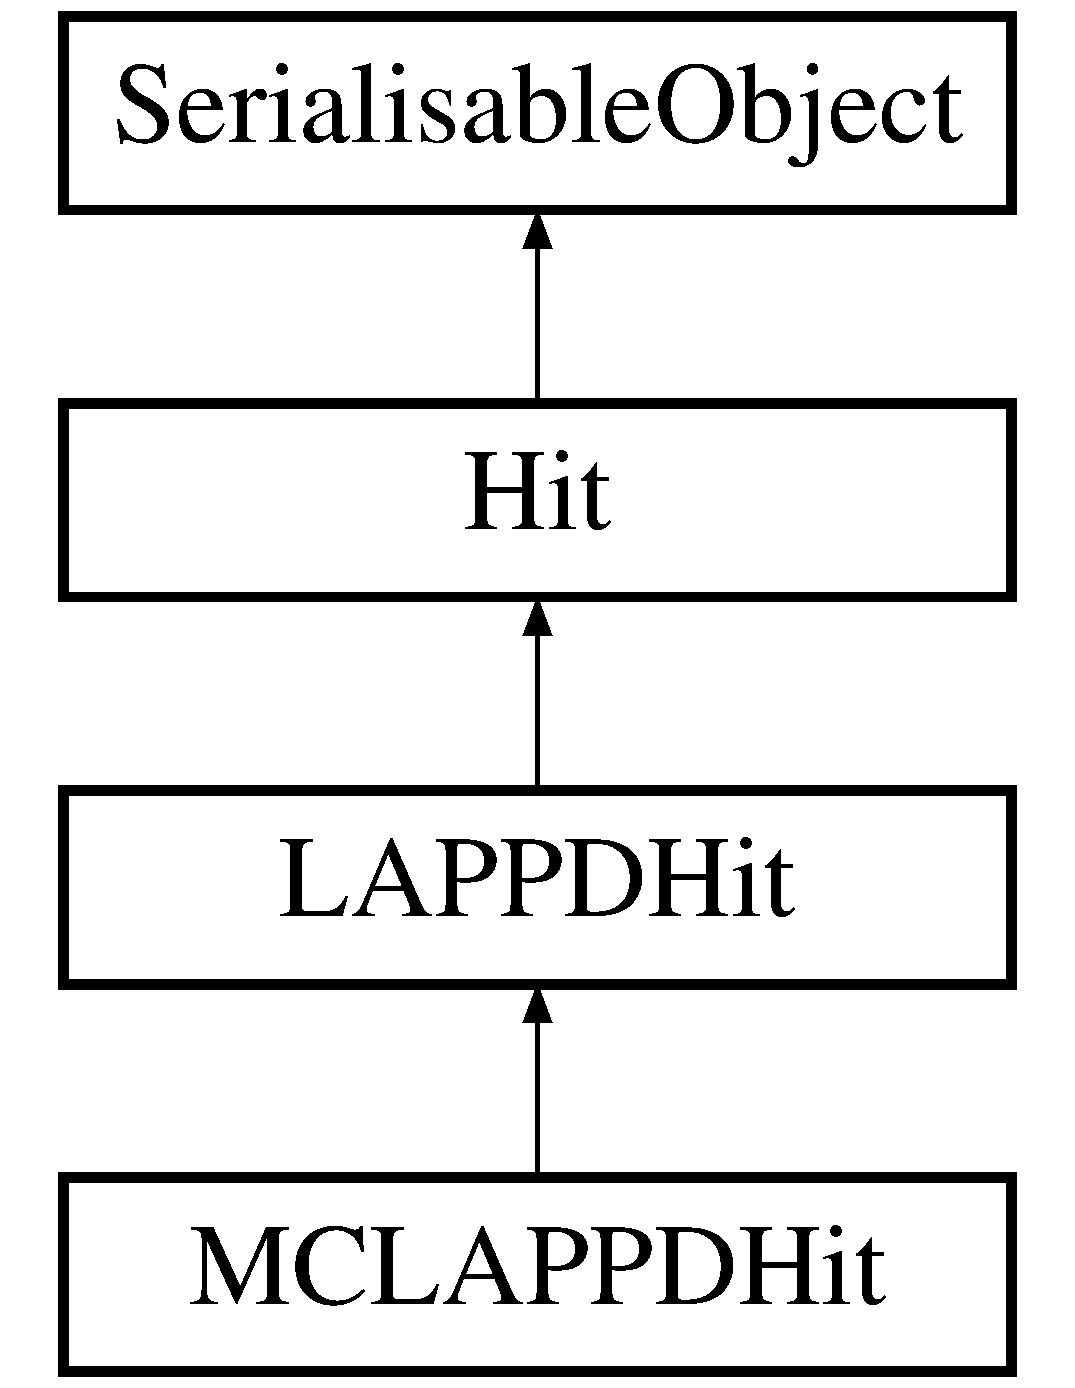
\includegraphics[height=4.000000cm]{classLAPPDHit}
\end{center}
\end{figure}
\subsection*{Public Member Functions}
\begin{DoxyCompactItemize}
\item 
\hypertarget{classLAPPDHit_afe5f8ccfdc8ea9c3cbf1ceb9c441e71d}{{\bfseries L\-A\-P\-P\-D\-Hit} (int thetubeid, double thetime, double thecharge, std\-::vector$<$ double $>$ theposition, std\-::vector$<$ double $>$ thelocalposition)}\label{classLAPPDHit_afe5f8ccfdc8ea9c3cbf1ceb9c441e71d}

\item 
\hypertarget{classLAPPDHit_ae1828d2ea7a97bc4fea858aaf94cedb4}{std\-::vector$<$ double $>$ {\bfseries Get\-Position} () const }\label{classLAPPDHit_ae1828d2ea7a97bc4fea858aaf94cedb4}

\item 
\hypertarget{classLAPPDHit_a9d1c4249ca261677004dbb0ea65effb1}{std\-::vector$<$ double $>$ {\bfseries Get\-Local\-Position} () const }\label{classLAPPDHit_a9d1c4249ca261677004dbb0ea65effb1}

\item 
\hypertarget{classLAPPDHit_acddccb2ec31fd46be236b32ede3a783b}{void {\bfseries Set\-Position} (std\-::vector$<$ double $>$ pos)}\label{classLAPPDHit_acddccb2ec31fd46be236b32ede3a783b}

\item 
\hypertarget{classLAPPDHit_a21e01043d24da9974933bbcfa2d23d3c}{void {\bfseries Set\-Local\-Position} (std\-::vector$<$ double $>$ locpos)}\label{classLAPPDHit_a21e01043d24da9974933bbcfa2d23d3c}

\item 
\hypertarget{classLAPPDHit_af993f8cd1441e7a37e8e1ca0e6890654}{bool {\bfseries Print} ()}\label{classLAPPDHit_af993f8cd1441e7a37e8e1ca0e6890654}

\end{DoxyCompactItemize}
\subsection*{Protected Member Functions}
\begin{DoxyCompactItemize}
\item 
\hypertarget{classLAPPDHit_af8eec8f466271e953f15dff64a172b26}{{\footnotesize template$<$class Archive $>$ }\\void {\bfseries serialize} (Archive \&ar, const unsigned int version)}\label{classLAPPDHit_af8eec8f466271e953f15dff64a172b26}

\end{DoxyCompactItemize}
\subsection*{Protected Attributes}
\begin{DoxyCompactItemize}
\item 
\hypertarget{classLAPPDHit_a979fc1e4b88cb77cac43c4dc3582ce3d}{std\-::vector$<$ double $>$ {\bfseries Position}}\label{classLAPPDHit_a979fc1e4b88cb77cac43c4dc3582ce3d}

\item 
\hypertarget{classLAPPDHit_a5517affe4e65ca692ce67160cd361d85}{std\-::vector$<$ double $>$ {\bfseries Local\-Position}}\label{classLAPPDHit_a5517affe4e65ca692ce67160cd361d85}

\end{DoxyCompactItemize}
\subsection*{Friends}
\begin{DoxyCompactItemize}
\item 
\hypertarget{classLAPPDHit_ac98d07dd8f7b70e16ccb9a01abf56b9c}{class {\bfseries boost\-::serialization\-::access}}\label{classLAPPDHit_ac98d07dd8f7b70e16ccb9a01abf56b9c}

\end{DoxyCompactItemize}


The documentation for this class was generated from the following file\-:\begin{DoxyCompactItemize}
\item 
Data\-Model/L\-A\-P\-P\-D\-Hit.\-h\end{DoxyCompactItemize}

\hypertarget{classLAPPDIntegratePulse}{\section{L\-A\-P\-P\-D\-Integrate\-Pulse Class Reference}
\label{classLAPPDIntegratePulse}\index{L\-A\-P\-P\-D\-Integrate\-Pulse@{L\-A\-P\-P\-D\-Integrate\-Pulse}}
}
Inheritance diagram for L\-A\-P\-P\-D\-Integrate\-Pulse\-:\begin{figure}[H]
\begin{center}
\leavevmode
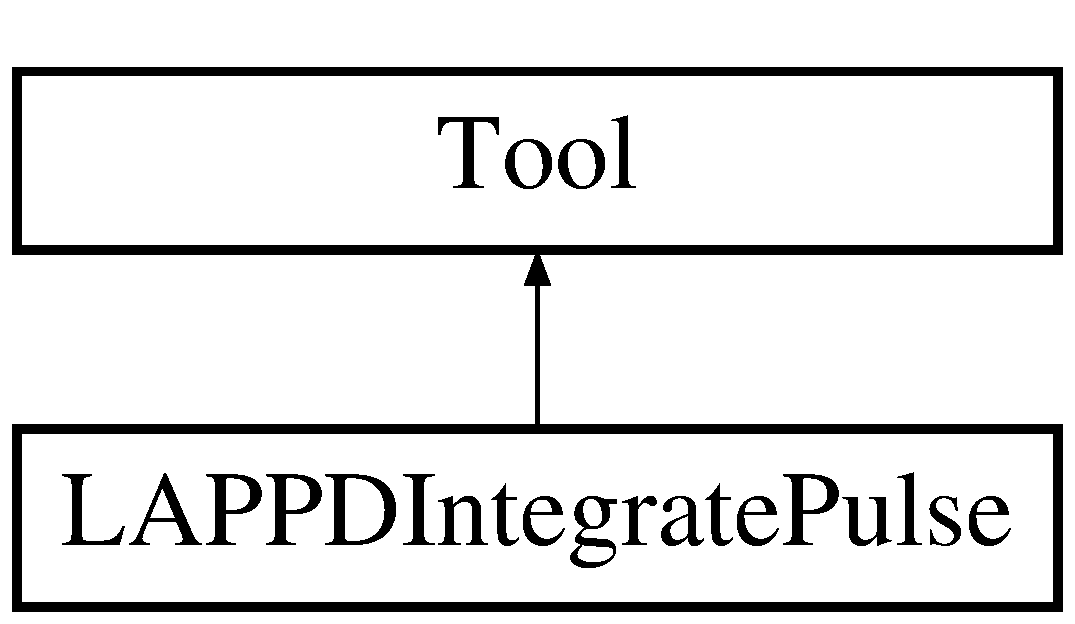
\includegraphics[height=2.000000cm]{classLAPPDIntegratePulse}
\end{center}
\end{figure}
\subsection*{Public Member Functions}
\begin{DoxyCompactItemize}
\item 
\hypertarget{classLAPPDIntegratePulse_ab68036bfa8f3ae98552907590df7d57a}{bool {\bfseries Initialise} (std\-::string configfile, \hyperlink{classDataModel}{Data\-Model} \&data)}\label{classLAPPDIntegratePulse_ab68036bfa8f3ae98552907590df7d57a}

\item 
\hypertarget{classLAPPDIntegratePulse_ada15e2fbf5c978255a848d0e8dce064a}{bool {\bfseries Execute} ()}\label{classLAPPDIntegratePulse_ada15e2fbf5c978255a848d0e8dce064a}

\item 
\hypertarget{classLAPPDIntegratePulse_ab17c0fe3193abd1970c6148049bacc18}{bool {\bfseries Finalise} ()}\label{classLAPPDIntegratePulse_ab17c0fe3193abd1970c6148049bacc18}

\end{DoxyCompactItemize}


The documentation for this class was generated from the following files\-:\begin{DoxyCompactItemize}
\item 
User\-Tools/\-L\-A\-P\-P\-D\-Integrate\-Pulse/L\-A\-P\-P\-D\-Integrate\-Pulse.\-h\item 
User\-Tools/\-L\-A\-P\-P\-D\-Integrate\-Pulse/L\-A\-P\-P\-D\-Integrate\-Pulse.\-cpp\end{DoxyCompactItemize}

\hypertarget{classLAPPDlasertestHitFinder}{
\section{LAPPDlasertestHitFinder Class Reference}
\label{classLAPPDlasertestHitFinder}\index{LAPPDlasertestHitFinder@{LAPPDlasertestHitFinder}}
}
\subsection*{Public Member Functions}
\begin{DoxyCompactItemize}
\item 
\hypertarget{classLAPPDlasertestHitFinder_a0a4dd1a750223833c9eb520008d4f821}{
bool {\bfseries Initialise} (std::string configfile, \hyperlink{classDataModel}{DataModel} \&data)}
\label{classLAPPDlasertestHitFinder_a0a4dd1a750223833c9eb520008d4f821}

\item 
\hypertarget{classLAPPDlasertestHitFinder_a028ed1741a9dd6048638a8e6f95f718a}{
bool {\bfseries Execute} ()}
\label{classLAPPDlasertestHitFinder_a028ed1741a9dd6048638a8e6f95f718a}

\item 
\hypertarget{classLAPPDlasertestHitFinder_a0ca3d1db237531ab1954a79f4ae469bd}{
bool {\bfseries Finalise} ()}
\label{classLAPPDlasertestHitFinder_a0ca3d1db237531ab1954a79f4ae469bd}

\end{DoxyCompactItemize}


The documentation for this class was generated from the following files:\begin{DoxyCompactItemize}
\item 
UserTools/LAPPDlasertestHitFinder/LAPPDlasertestHitFinder.h\item 
UserTools/LAPPDlasertestHitFinder/LAPPDlasertestHitFinder.cpp\end{DoxyCompactItemize}

\hypertarget{classLAPPDParseACC}{\section{L\-A\-P\-P\-D\-Parse\-A\-C\-C Class Reference}
\label{classLAPPDParseACC}\index{L\-A\-P\-P\-D\-Parse\-A\-C\-C@{L\-A\-P\-P\-D\-Parse\-A\-C\-C}}
}
Inheritance diagram for L\-A\-P\-P\-D\-Parse\-A\-C\-C\-:\begin{figure}[H]
\begin{center}
\leavevmode
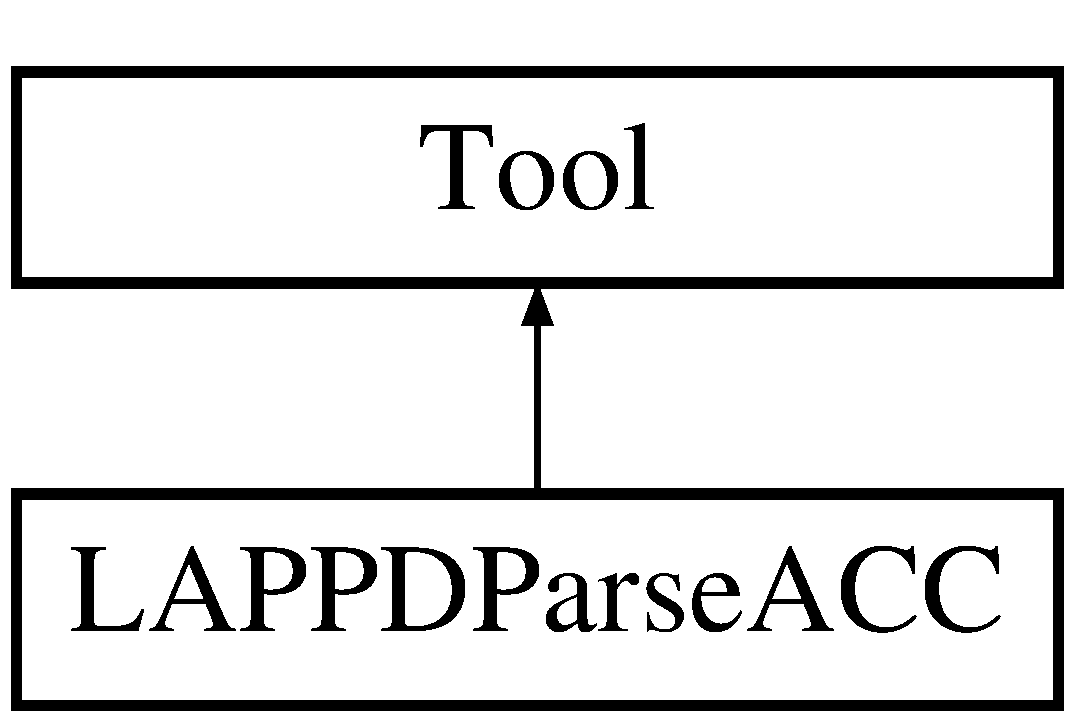
\includegraphics[height=2.000000cm]{classLAPPDParseACC}
\end{center}
\end{figure}
\subsection*{Public Member Functions}
\begin{DoxyCompactItemize}
\item 
\hypertarget{classLAPPDParseACC_acb7a9ca57ebef424c67ee6b2452c865e}{bool {\bfseries Initialise} (std\-::string configfile, \hyperlink{classDataModel}{Data\-Model} \&data)}\label{classLAPPDParseACC_acb7a9ca57ebef424c67ee6b2452c865e}

\item 
\hypertarget{classLAPPDParseACC_a398f4910f5179cc7463302c52a7280fb}{bool {\bfseries Execute} ()}\label{classLAPPDParseACC_a398f4910f5179cc7463302c52a7280fb}

\item 
\hypertarget{classLAPPDParseACC_a27d71df3f3481f978a819ea1830367ae}{bool {\bfseries Finalise} ()}\label{classLAPPDParseACC_a27d71df3f3481f978a819ea1830367ae}

\end{DoxyCompactItemize}


The documentation for this class was generated from the following files\-:\begin{DoxyCompactItemize}
\item 
User\-Tools/\-L\-A\-P\-P\-D\-Parse\-A\-C\-C/L\-A\-P\-P\-D\-Parse\-A\-C\-C.\-h\item 
User\-Tools/\-L\-A\-P\-P\-D\-Parse\-A\-C\-C/L\-A\-P\-P\-D\-Parse\-A\-C\-C.\-cpp\end{DoxyCompactItemize}

\hypertarget{classLAPPDParseScope}{\section{L\-A\-P\-P\-D\-Parse\-Scope Class Reference}
\label{classLAPPDParseScope}\index{L\-A\-P\-P\-D\-Parse\-Scope@{L\-A\-P\-P\-D\-Parse\-Scope}}
}
Inheritance diagram for L\-A\-P\-P\-D\-Parse\-Scope\-:\begin{figure}[H]
\begin{center}
\leavevmode
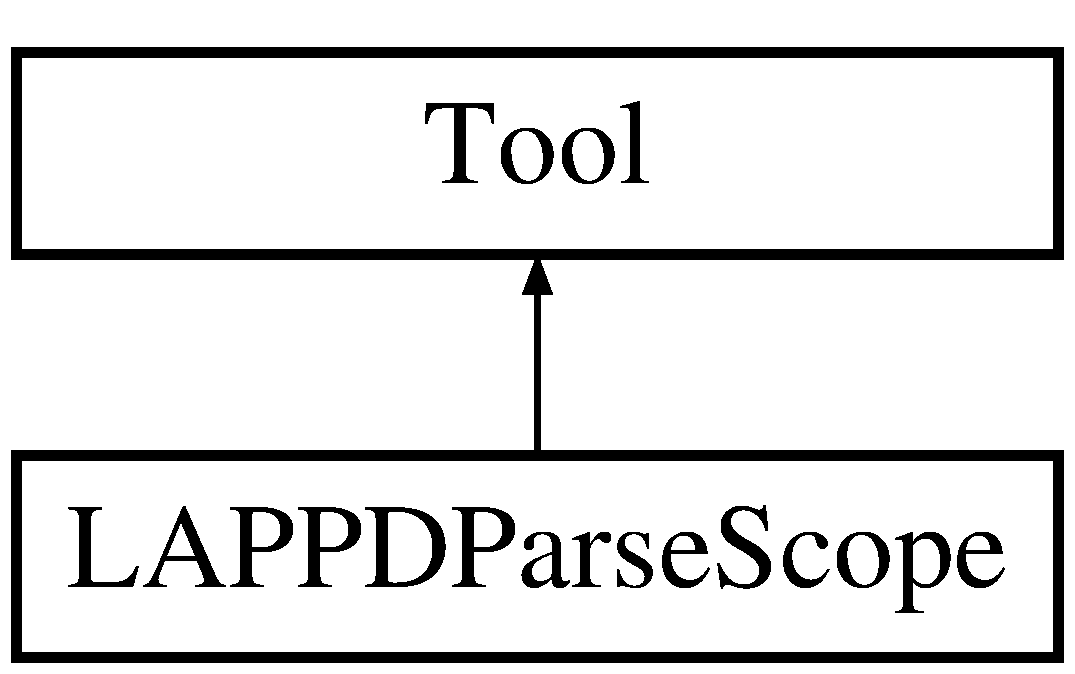
\includegraphics[height=2.000000cm]{classLAPPDParseScope}
\end{center}
\end{figure}
\subsection*{Public Member Functions}
\begin{DoxyCompactItemize}
\item 
\hypertarget{classLAPPDParseScope_a5b2511aa79384f73240784028b39d427}{bool {\bfseries Initialise} (std\-::string configfile, \hyperlink{classDataModel}{Data\-Model} \&data)}\label{classLAPPDParseScope_a5b2511aa79384f73240784028b39d427}

\item 
\hypertarget{classLAPPDParseScope_ade2b40ff4ad384ab3778cb991bde62b6}{bool {\bfseries Execute} ()}\label{classLAPPDParseScope_ade2b40ff4ad384ab3778cb991bde62b6}

\item 
\hypertarget{classLAPPDParseScope_a7582fc226353ddceea5a73ff48d8c6a1}{bool {\bfseries Finalise} ()}\label{classLAPPDParseScope_a7582fc226353ddceea5a73ff48d8c6a1}

\end{DoxyCompactItemize}


The documentation for this class was generated from the following files\-:\begin{DoxyCompactItemize}
\item 
User\-Tools/\-L\-A\-P\-P\-D\-Parse\-Scope/L\-A\-P\-P\-D\-Parse\-Scope.\-h\item 
User\-Tools/\-L\-A\-P\-P\-D\-Parse\-Scope/L\-A\-P\-P\-D\-Parse\-Scope.\-cpp\end{DoxyCompactItemize}

\hypertarget{classLAPPDPulse}{\section{L\-A\-P\-P\-D\-Pulse Class Reference}
\label{classLAPPDPulse}\index{L\-A\-P\-P\-D\-Pulse@{L\-A\-P\-P\-D\-Pulse}}
}
Inheritance diagram for L\-A\-P\-P\-D\-Pulse\-:\begin{figure}[H]
\begin{center}
\leavevmode
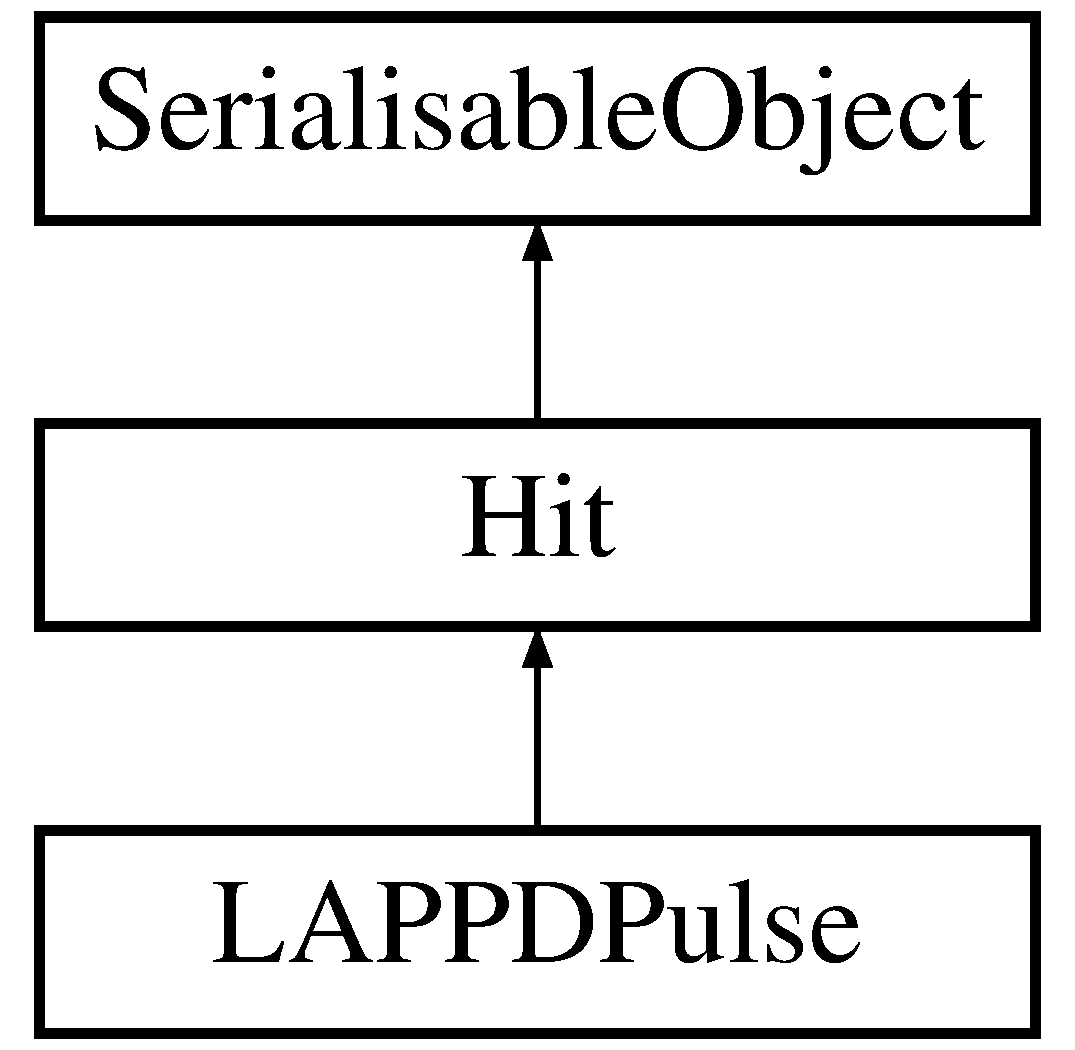
\includegraphics[height=3.000000cm]{classLAPPDPulse}
\end{center}
\end{figure}
\subsection*{Public Member Functions}
\begin{DoxyCompactItemize}
\item 
\hypertarget{classLAPPDPulse_ab6d60a683e420fd6304cc8d06b56e3f6}{{\bfseries L\-A\-P\-P\-D\-Pulse} (int tubeid, int channelid, double thetime, double charge, double peak, double low, double hi)}\label{classLAPPDPulse_ab6d60a683e420fd6304cc8d06b56e3f6}

\item 
\hypertarget{classLAPPDPulse_af0a8fed16c7b5c00f8bb644fb5b5a862}{int {\bfseries Get\-Channel\-I\-D} ()}\label{classLAPPDPulse_af0a8fed16c7b5c00f8bb644fb5b5a862}

\item 
\hypertarget{classLAPPDPulse_a86ef7d81b63accf60eea72dffd3c578d}{double {\bfseries Get\-Peak} ()}\label{classLAPPDPulse_a86ef7d81b63accf60eea72dffd3c578d}

\item 
\hypertarget{classLAPPDPulse_ac60601aee23092e71c13b953415d9d6d}{double {\bfseries Get\-Low\-Range} ()}\label{classLAPPDPulse_ac60601aee23092e71c13b953415d9d6d}

\item 
\hypertarget{classLAPPDPulse_a471f03a01ed49ef0db9438d13fe12200}{double {\bfseries Get\-Hi\-Range} ()}\label{classLAPPDPulse_a471f03a01ed49ef0db9438d13fe12200}

\item 
\hypertarget{classLAPPDPulse_ae3dad03fc206ae35ad7799ffe892f949}{void {\bfseries Set\-Channel\-I\-D} (int channelid)}\label{classLAPPDPulse_ae3dad03fc206ae35ad7799ffe892f949}

\item 
\hypertarget{classLAPPDPulse_a0c08b4bd1739552c7d6e2ad8cd9541e5}{void {\bfseries Set\-Peak} (double peak)}\label{classLAPPDPulse_a0c08b4bd1739552c7d6e2ad8cd9541e5}

\item 
\hypertarget{classLAPPDPulse_ae9345baa2efd05784e2b5c3c7023c194}{void {\bfseries Set\-Range} (double low, double hi)}\label{classLAPPDPulse_ae9345baa2efd05784e2b5c3c7023c194}

\item 
\hypertarget{classLAPPDPulse_a96fde20895fdcf61eb055308ed0b962d}{bool {\bfseries Print} ()}\label{classLAPPDPulse_a96fde20895fdcf61eb055308ed0b962d}

\end{DoxyCompactItemize}
\subsection*{Protected Member Functions}
\begin{DoxyCompactItemize}
\item 
\hypertarget{classLAPPDPulse_aa51fb4050ecce1aca2beb008a272d766}{{\footnotesize template$<$class Archive $>$ }\\void {\bfseries serialize} (Archive \&ar, const unsigned int version)}\label{classLAPPDPulse_aa51fb4050ecce1aca2beb008a272d766}

\end{DoxyCompactItemize}
\subsection*{Protected Attributes}
\begin{DoxyCompactItemize}
\item 
\hypertarget{classLAPPDPulse_a2e42975bd2fd735b7bd7d7c2bacb683f}{double {\bfseries Channel\-I\-D}}\label{classLAPPDPulse_a2e42975bd2fd735b7bd7d7c2bacb683f}

\item 
\hypertarget{classLAPPDPulse_a72893cf5f3accbe429e2cb1437b02064}{double {\bfseries Peak}}\label{classLAPPDPulse_a72893cf5f3accbe429e2cb1437b02064}

\item 
\hypertarget{classLAPPDPulse_af4923695ff523930e7109fab7743d7c4}{double {\bfseries Low\-Range}}\label{classLAPPDPulse_af4923695ff523930e7109fab7743d7c4}

\item 
\hypertarget{classLAPPDPulse_a5ee5c47716e498114b8924a64a92b562}{double {\bfseries Hi\-Range}}\label{classLAPPDPulse_a5ee5c47716e498114b8924a64a92b562}

\end{DoxyCompactItemize}
\subsection*{Friends}
\begin{DoxyCompactItemize}
\item 
\hypertarget{classLAPPDPulse_ac98d07dd8f7b70e16ccb9a01abf56b9c}{class {\bfseries boost\-::serialization\-::access}}\label{classLAPPDPulse_ac98d07dd8f7b70e16ccb9a01abf56b9c}

\end{DoxyCompactItemize}


The documentation for this class was generated from the following file\-:\begin{DoxyCompactItemize}
\item 
Data\-Model/L\-A\-P\-P\-D\-Pulse.\-h\end{DoxyCompactItemize}

\hypertarget{classLAPPDresponse}{\section{L\-A\-P\-P\-Dresponse Class Reference}
\label{classLAPPDresponse}\index{L\-A\-P\-P\-Dresponse@{L\-A\-P\-P\-Dresponse}}
}
\subsection*{Public Member Functions}
\begin{DoxyCompactItemize}
\item 
\hypertarget{classLAPPDresponse_a5d53c8ca94cd0b1d2f389df41b3c71d0}{void {\bfseries Add\-Single\-Photon\-Trace} (double trans, double para, double time)}\label{classLAPPDresponse_a5d53c8ca94cd0b1d2f389df41b3c71d0}

\item 
\hypertarget{classLAPPDresponse_a6dc34922a8a63dc84fa2758ad7ae07f5}{\hyperlink{classWaveform}{Waveform}$<$ double $>$ {\bfseries Get\-Trace} (int C\-Hnumber, double starttime, double samplesize, int numsamples, double thenoise)}\label{classLAPPDresponse_a6dc34922a8a63dc84fa2758ad7ae07f5}

\item 
\hypertarget{classLAPPDresponse_af7ea4eaf42b67cd816a1205c84e9756b}{int {\bfseries Find\-Strip\-Number} (double trans)}\label{classLAPPDresponse_af7ea4eaf42b67cd816a1205c84e9756b}

\item 
\hypertarget{classLAPPDresponse_a7006a41063a44bec116b5763dfd218ac}{double {\bfseries Strip\-Coordinate} (int stripnumber)}\label{classLAPPDresponse_a7006a41063a44bec116b5763dfd218ac}

\item 
\hypertarget{classLAPPDresponse_a5d53c8ca94cd0b1d2f389df41b3c71d0}{void {\bfseries Add\-Single\-Photon\-Trace} (double trans, double para, double time)}\label{classLAPPDresponse_a5d53c8ca94cd0b1d2f389df41b3c71d0}

\item 
\hypertarget{classLAPPDresponse_adcf4b1cb461f805e4f2b0106ad24a87d}{\hyperlink{classWaveform}{Waveform}$<$ double $>$ {\bfseries Get\-Trace} (int C\-Hnumber, double starttime, double samplesize, int numsamples, double thenoise)}\label{classLAPPDresponse_adcf4b1cb461f805e4f2b0106ad24a87d}

\item 
\hypertarget{classLAPPDresponse_af7ea4eaf42b67cd816a1205c84e9756b}{int {\bfseries Find\-Strip\-Number} (double trans)}\label{classLAPPDresponse_af7ea4eaf42b67cd816a1205c84e9756b}

\item 
\hypertarget{classLAPPDresponse_a7006a41063a44bec116b5763dfd218ac}{double {\bfseries Strip\-Coordinate} (int stripnumber)}\label{classLAPPDresponse_a7006a41063a44bec116b5763dfd218ac}

\end{DoxyCompactItemize}
\subsection*{Public Attributes}
\begin{DoxyCompactItemize}
\item 
\hypertarget{classLAPPDresponse_ae10b5dcda1903b993df6891d60b1e0d4}{map$<$ int, vector$<$ \hyperlink{classLAPPDPulse}{L\-A\-P\-P\-D\-Pulse} $>$ $>$ {\bfseries L\-A\-P\-P\-D\-Pulse\-Cluster}}\label{classLAPPDresponse_ae10b5dcda1903b993df6891d60b1e0d4}

\end{DoxyCompactItemize}


The documentation for this class was generated from the following files\-:\begin{DoxyCompactItemize}
\item 
User\-Tools/\-Histograms\-Root\-L\-A\-P\-P\-D\-Data/L\-A\-P\-P\-Dresponse.\-hh\item 
User\-Tools/\-L\-A\-P\-P\-D\-Sim/L\-A\-P\-P\-Dresponse.\-hh\item 
User\-Tools/\-L\-A\-P\-P\-D\-Sim/L\-A\-P\-P\-Dresponse.\-cpp\end{DoxyCompactItemize}

\hypertarget{classLAPPDSim}{\section{L\-A\-P\-P\-D\-Sim Class Reference}
\label{classLAPPDSim}\index{L\-A\-P\-P\-D\-Sim@{L\-A\-P\-P\-D\-Sim}}
}
Inheritance diagram for L\-A\-P\-P\-D\-Sim\-:\begin{figure}[H]
\begin{center}
\leavevmode
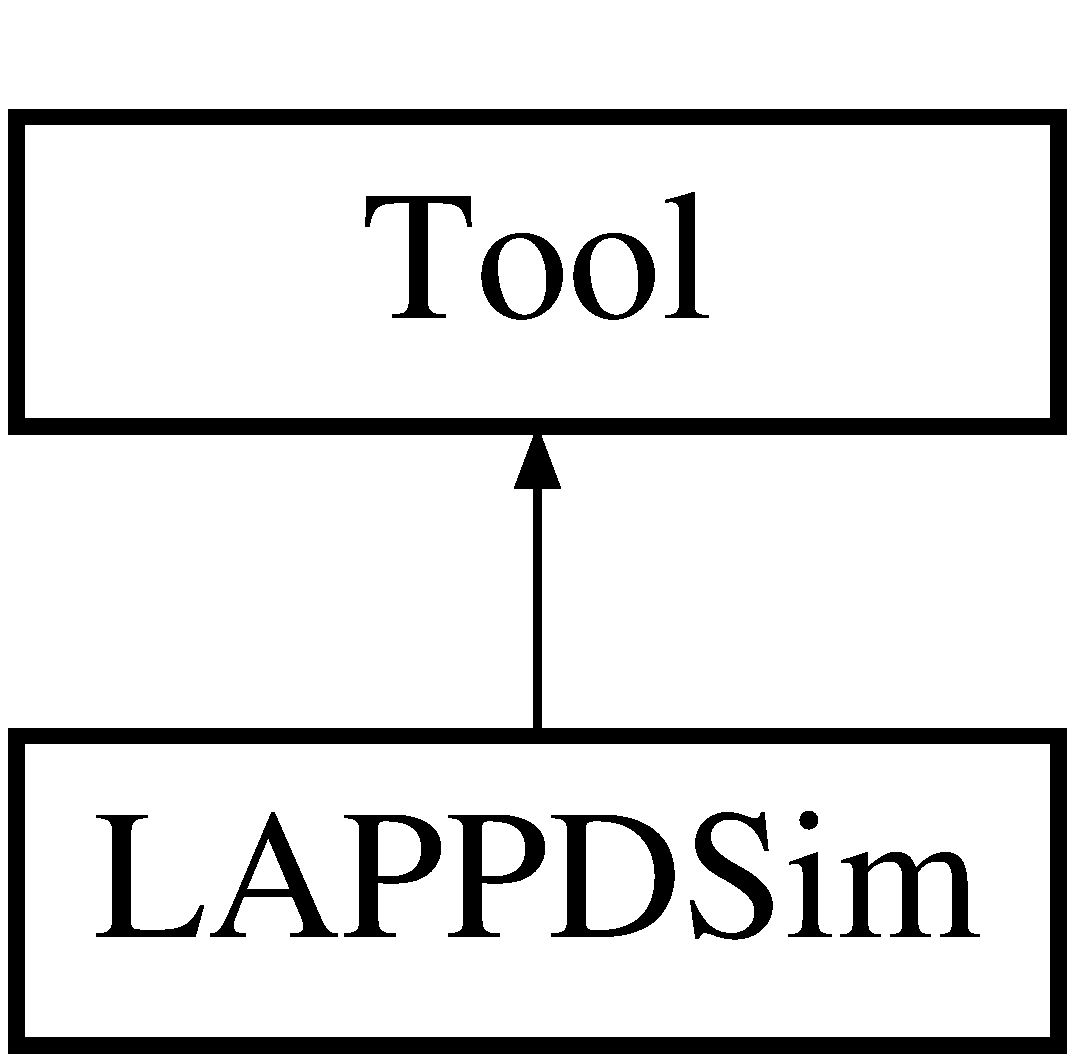
\includegraphics[height=2.000000cm]{classLAPPDSim}
\end{center}
\end{figure}
\subsection*{Public Member Functions}
\begin{DoxyCompactItemize}
\item 
\hypertarget{classLAPPDSim_a68edcbace6d4b83bff31e3866d0cbfc1}{bool {\bfseries Initialise} (std\-::string configfile, \hyperlink{classDataModel}{Data\-Model} \&data)}\label{classLAPPDSim_a68edcbace6d4b83bff31e3866d0cbfc1}

\item 
\hypertarget{classLAPPDSim_a0d34e153938d2a1c6fab9c3083862000}{bool {\bfseries Execute} ()}\label{classLAPPDSim_a0d34e153938d2a1c6fab9c3083862000}

\item 
\hypertarget{classLAPPDSim_a97d903656a7ddbdafb5170bb672193ba}{bool {\bfseries Finalise} ()}\label{classLAPPDSim_a97d903656a7ddbdafb5170bb672193ba}

\item 
\hypertarget{classLAPPDSim_ab08ad145a8cea2e3d0283ba48b91fa47}{\hyperlink{classWaveform}{Waveform}$<$ double $>$ {\bfseries Simple\-Gen\-Pulse} (vector$<$ double $>$ pulsetimes)}\label{classLAPPDSim_ab08ad145a8cea2e3d0283ba48b91fa47}

\end{DoxyCompactItemize}


The documentation for this class was generated from the following files\-:\begin{DoxyCompactItemize}
\item 
User\-Tools/\-L\-A\-P\-P\-D\-Sim/L\-A\-P\-P\-D\-Sim.\-h\item 
User\-Tools/\-L\-A\-P\-P\-D\-Sim/L\-A\-P\-P\-D\-Sim.\-cpp\end{DoxyCompactItemize}

\hypertarget{classLAPPDTree}{\section{L\-A\-P\-P\-D\-Tree Class Reference}
\label{classLAPPDTree}\index{L\-A\-P\-P\-D\-Tree@{L\-A\-P\-P\-D\-Tree}}
}
\subsection*{Public Member Functions}
\begin{DoxyCompactItemize}
\item 
\hypertarget{classLAPPDTree_abb24c0d515c12bc1809d5d0bf7c6abc6}{{\bfseries L\-A\-P\-P\-D\-Tree} (T\-Tree $\ast$tree=0)}\label{classLAPPDTree_abb24c0d515c12bc1809d5d0bf7c6abc6}

\item 
\hypertarget{classLAPPDTree_a1f59d9cca524a5cc0a9a8c525b94d1b1}{{\bfseries L\-A\-P\-P\-D\-Tree} (const char $\ast$filepath, bool addsubdirs)}\label{classLAPPDTree_a1f59d9cca524a5cc0a9a8c525b94d1b1}

\item 
\hypertarget{classLAPPDTree_a6de6bc7aa0dbf3bb246fbaae06723244}{virtual Int\-\_\-t {\bfseries Cut} (Long64\-\_\-t entry)}\label{classLAPPDTree_a6de6bc7aa0dbf3bb246fbaae06723244}

\item 
\hypertarget{classLAPPDTree_a0ae74d3f6b190e015bc109d039f4f9a8}{virtual Int\-\_\-t {\bfseries Get\-Entry} (Long64\-\_\-t entry)}\label{classLAPPDTree_a0ae74d3f6b190e015bc109d039f4f9a8}

\item 
\hypertarget{classLAPPDTree_a9047fa387962f63c3da57a5fe9dd31e1}{virtual Long64\-\_\-t {\bfseries Load\-Tree} (Long64\-\_\-t entry)}\label{classLAPPDTree_a9047fa387962f63c3da57a5fe9dd31e1}

\item 
\hypertarget{classLAPPDTree_a347e8109500ef62ace4bbc0d89890918}{virtual void {\bfseries Init} (T\-Tree $\ast$tree)}\label{classLAPPDTree_a347e8109500ef62ace4bbc0d89890918}

\item 
\hypertarget{classLAPPDTree_ad16b2af53b7d2ab9a2f63514cd0de6b4}{virtual void {\bfseries Loop} ()}\label{classLAPPDTree_ad16b2af53b7d2ab9a2f63514cd0de6b4}

\item 
\hypertarget{classLAPPDTree_a404d7028c21e7c2e0c6339b917c3ca67}{virtual Bool\-\_\-t {\bfseries Notify} ()}\label{classLAPPDTree_a404d7028c21e7c2e0c6339b917c3ca67}

\item 
\hypertarget{classLAPPDTree_a7d7520170ee101a91a5003e09b55c9a6}{virtual void {\bfseries Show} (Long64\-\_\-t entry=-\/1)}\label{classLAPPDTree_a7d7520170ee101a91a5003e09b55c9a6}

\item 
\hypertarget{classLAPPDTree_aa2436cb85efeec18ff4e05c9fda41359}{T\-Chain $\ast$ {\bfseries Add\-Files} (const char $\ast$inputdir, bool addsubfolders)}\label{classLAPPDTree_aa2436cb85efeec18ff4e05c9fda41359}

\end{DoxyCompactItemize}
\subsection*{Public Attributes}
\begin{DoxyCompactItemize}
\item 
\hypertarget{classLAPPDTree_ab7334c305d8c67c1469b286cd775845c}{T\-Tree $\ast$ {\bfseries f\-Chain}}\label{classLAPPDTree_ab7334c305d8c67c1469b286cd775845c}

\item 
\hypertarget{classLAPPDTree_a57ea0164e27a936105e60d5a7910335d}{Int\-\_\-t \hyperlink{classLAPPDTree_a57ea0164e27a936105e60d5a7910335d}{f\-Current}}\label{classLAPPDTree_a57ea0164e27a936105e60d5a7910335d}

\begin{DoxyCompactList}\small\item\em pointer to the analyzed T\-Tree or T\-Chain \end{DoxyCompactList}\item 
\hypertarget{classLAPPDTree_af6c1ba92cb9a0f70418af64563f7bccf}{int \hyperlink{classLAPPDTree_af6c1ba92cb9a0f70418af64563f7bccf}{verbose} =1}\label{classLAPPDTree_af6c1ba92cb9a0f70418af64563f7bccf}

\begin{DoxyCompactList}\small\item\em current Tree number in a T\-Chain \end{DoxyCompactList}\item 
\hypertarget{classLAPPDTree_a3a198c1cfd76e782b371ae2eddc911d7}{Int\-\_\-t {\bfseries lappdevt}}\label{classLAPPDTree_a3a198c1cfd76e782b371ae2eddc911d7}

\item 
\hypertarget{classLAPPDTree_a82b4e313a76045692cad281c966955b8}{Int\-\_\-t {\bfseries lappd\-\_\-numhits}}\label{classLAPPDTree_a82b4e313a76045692cad281c966955b8}

\item 
\hypertarget{classLAPPDTree_a92a142c36821ddf3a0dc240d57ace54f}{Int\-\_\-t {\bfseries lappdhit\-\_\-objnum} \mbox{[}180\mbox{]}}\label{classLAPPDTree_a92a142c36821ddf3a0dc240d57ace54f}

\item 
\hypertarget{classLAPPDTree_a7dbf3acc22501e676eac167d1c8bfb91}{Double\-\_\-t {\bfseries lappdhit\-\_\-x} \mbox{[}180\mbox{]}}\label{classLAPPDTree_a7dbf3acc22501e676eac167d1c8bfb91}

\item 
\hypertarget{classLAPPDTree_a2bc97b493024b71430528a71c2339ec7}{Double\-\_\-t {\bfseries lappdhit\-\_\-y} \mbox{[}180\mbox{]}}\label{classLAPPDTree_a2bc97b493024b71430528a71c2339ec7}

\item 
\hypertarget{classLAPPDTree_a73e138836f63b843c99fbe3951f7e504}{Double\-\_\-t {\bfseries lappdhit\-\_\-z} \mbox{[}180\mbox{]}}\label{classLAPPDTree_a73e138836f63b843c99fbe3951f7e504}

\item 
\hypertarget{classLAPPDTree_aa5f1d299a73e165905b798a925206de5}{vector$<$ double $>$ $\ast$ {\bfseries lappdhit\-\_\-stripcoorx}}\label{classLAPPDTree_aa5f1d299a73e165905b798a925206de5}

\item 
\hypertarget{classLAPPDTree_a1a9420e83fa6ac964448bd89fb613248}{vector$<$ double $>$ $\ast$ {\bfseries lappdhit\-\_\-stripcoory}}\label{classLAPPDTree_a1a9420e83fa6ac964448bd89fb613248}

\item 
\hypertarget{classLAPPDTree_a07b7a60f594d559022c75cc8962a673e}{vector$<$ double $>$ $\ast$ {\bfseries lappdhit\-\_\-stripcoort}}\label{classLAPPDTree_a07b7a60f594d559022c75cc8962a673e}

\item 
\hypertarget{classLAPPDTree_a361c88caa35c7b75c6625d1726fd3116}{Double\-\_\-t {\bfseries lappdhit\-\_\-edep} \mbox{[}180\mbox{]}}\label{classLAPPDTree_a361c88caa35c7b75c6625d1726fd3116}

\item 
\hypertarget{classLAPPDTree_abbf80a1da763ec467ead614fd4289718}{vector$<$ double $>$ $\ast$ {\bfseries lappdhit\-\_\-globalcoorx}}\label{classLAPPDTree_abbf80a1da763ec467ead614fd4289718}

\item 
\hypertarget{classLAPPDTree_a4d4353d05db2632541d8a34b825cc5e8}{vector$<$ double $>$ $\ast$ {\bfseries lappdhit\-\_\-globalcoory}}\label{classLAPPDTree_a4d4353d05db2632541d8a34b825cc5e8}

\item 
\hypertarget{classLAPPDTree_a44dc4554d5ea50fe0043d6d5e83292d4}{vector$<$ double $>$ $\ast$ {\bfseries lappdhit\-\_\-globalcoorz}}\label{classLAPPDTree_a44dc4554d5ea50fe0043d6d5e83292d4}

\item 
\hypertarget{classLAPPDTree_a842bd00c916ff704c337885e944a2597}{vector$<$ double $>$ {\bfseries lappdhit\-\_\-globalcoorxdummy}}\label{classLAPPDTree_a842bd00c916ff704c337885e944a2597}

\item 
\hypertarget{classLAPPDTree_a43f80af2bdabd39c31346a526b8e9a5c}{vector$<$ double $>$ {\bfseries lappdhit\-\_\-globalcoorydummy}}\label{classLAPPDTree_a43f80af2bdabd39c31346a526b8e9a5c}

\item 
\hypertarget{classLAPPDTree_a9ed8c2c3aa42ecc9fbaa575caa076940}{vector$<$ double $>$ {\bfseries lappdhit\-\_\-globalcoorzdummy}}\label{classLAPPDTree_a9ed8c2c3aa42ecc9fbaa575caa076940}

\item 
\hypertarget{classLAPPDTree_a372097f371b2bbd414b6447da2e5fd51}{vector$<$ int $>$ $\ast$ {\bfseries lappdhit\-\_\-primary\-Parent\-I\-D2}}\label{classLAPPDTree_a372097f371b2bbd414b6447da2e5fd51}

\item 
\hypertarget{classLAPPDTree_af47a619c8a87743efecb91b7fbf2c7be}{T\-Branch $\ast$ {\bfseries b\-\_\-lappdevt}}\label{classLAPPDTree_af47a619c8a87743efecb91b7fbf2c7be}

\item 
\hypertarget{classLAPPDTree_af2d3bcf8ac6d1984ddd5da708841fd81}{T\-Branch $\ast$ {\bfseries b\-\_\-lappd\-\_\-numhits}}\label{classLAPPDTree_af2d3bcf8ac6d1984ddd5da708841fd81}

\item 
\hypertarget{classLAPPDTree_aaffff4e3fa3c778499625bc2c79179de}{T\-Branch $\ast$ {\bfseries b\-\_\-lappdhit\-\_\-totalpes\-\_\-perevt}}\label{classLAPPDTree_aaffff4e3fa3c778499625bc2c79179de}

\item 
\hypertarget{classLAPPDTree_a97ffd58d9a74db4d2026aea619e55c3e}{T\-Branch $\ast$ {\bfseries b\-\_\-lappdhit\-\_\-totalpes\-\_\-perlappd2}}\label{classLAPPDTree_a97ffd58d9a74db4d2026aea619e55c3e}

\item 
\hypertarget{classLAPPDTree_aaa3ff0b6eefee590df4209064eb2907f}{T\-Branch $\ast$ {\bfseries b\-\_\-lappdhit\-\_\-x}}\label{classLAPPDTree_aaa3ff0b6eefee590df4209064eb2907f}

\item 
\hypertarget{classLAPPDTree_adc45ffd7b8f116526d1683182a8b0104}{T\-Branch $\ast$ {\bfseries b\-\_\-lappdhit\-\_\-y}}\label{classLAPPDTree_adc45ffd7b8f116526d1683182a8b0104}

\item 
\hypertarget{classLAPPDTree_ac15eb6f5a771b3a8a4af9f98ef64642c}{T\-Branch $\ast$ {\bfseries b\-\_\-lappdhit\-\_\-z}}\label{classLAPPDTree_ac15eb6f5a771b3a8a4af9f98ef64642c}

\item 
\hypertarget{classLAPPDTree_a321a08fed926fdb6e506cf99e3036932}{T\-Branch $\ast$ {\bfseries b\-\_\-lappdhit\-\_\-stripcoorx}}\label{classLAPPDTree_a321a08fed926fdb6e506cf99e3036932}

\item 
\hypertarget{classLAPPDTree_a08b0df3f4c28158e497a5d54b4c52646}{T\-Branch $\ast$ {\bfseries b\-\_\-lappdhit\-\_\-stripcoory}}\label{classLAPPDTree_a08b0df3f4c28158e497a5d54b4c52646}

\item 
\hypertarget{classLAPPDTree_af7b4cf0126506fa7159848c569bd9a0b}{T\-Branch $\ast$ {\bfseries b\-\_\-lappdhit\-\_\-stripcoorz}}\label{classLAPPDTree_af7b4cf0126506fa7159848c569bd9a0b}

\item 
\hypertarget{classLAPPDTree_a825861f9f2cc7aae1554b316ef8d39a9}{T\-Branch $\ast$ {\bfseries b\-\_\-lappdhit\-\_\-stripcoort}}\label{classLAPPDTree_a825861f9f2cc7aae1554b316ef8d39a9}

\item 
\hypertarget{classLAPPDTree_a2f1588991d3a64b51f09aad302903044}{T\-Branch $\ast$ {\bfseries b\-\_\-lappdhit\-\_\-globalcoorx}}\label{classLAPPDTree_a2f1588991d3a64b51f09aad302903044}

\item 
\hypertarget{classLAPPDTree_a1f5965eb70d5028bae942cd81ebf6820}{T\-Branch $\ast$ {\bfseries b\-\_\-lappdhit\-\_\-globalcoory}}\label{classLAPPDTree_a1f5965eb70d5028bae942cd81ebf6820}

\item 
\hypertarget{classLAPPDTree_a023ec732a7f88e6daca5480adff51a29}{T\-Branch $\ast$ {\bfseries b\-\_\-lappdhit\-\_\-globalcoorz}}\label{classLAPPDTree_a023ec732a7f88e6daca5480adff51a29}

\item 
\hypertarget{classLAPPDTree_ab0e08ad50302af8e404f4e133a8e7357}{T\-Branch $\ast$ {\bfseries b\-\_\-lappdhit\-\_\-process}}\label{classLAPPDTree_ab0e08ad50302af8e404f4e133a8e7357}

\item 
\hypertarget{classLAPPDTree_aee5aea4ed12b28c5784e951ab9004e4b}{T\-Branch $\ast$ {\bfseries b\-\_\-lappdhit\-\_\-particle\-I\-D}}\label{classLAPPDTree_aee5aea4ed12b28c5784e951ab9004e4b}

\item 
\hypertarget{classLAPPDTree_a4d9f69bbc84a59dd42763349fb5abfc5}{T\-Branch $\ast$ {\bfseries b\-\_\-lappdhit\-\_\-track\-I\-D}}\label{classLAPPDTree_a4d9f69bbc84a59dd42763349fb5abfc5}

\item 
\hypertarget{classLAPPDTree_aa1dde2f8ca08d72d9f6ef2614935909f}{T\-Branch $\ast$ {\bfseries b\-\_\-lappdhit\-\_\-edep}}\label{classLAPPDTree_aa1dde2f8ca08d72d9f6ef2614935909f}

\item 
\hypertarget{classLAPPDTree_a8f6eea3420011bb1a15307d4ab38c8fd}{T\-Branch $\ast$ {\bfseries b\-\_\-lappdhit\-\_\-objnum}}\label{classLAPPDTree_a8f6eea3420011bb1a15307d4ab38c8fd}

\item 
\hypertarget{classLAPPDTree_a719cbac920cf65ff67af978dfbac12d2}{T\-Branch $\ast$ {\bfseries b\-\_\-lappdhit\-\_\-stripnum}}\label{classLAPPDTree_a719cbac920cf65ff67af978dfbac12d2}

\item 
\hypertarget{classLAPPDTree_a3ba0a48b444731d20574179863c896a6}{T\-Branch $\ast$ {\bfseries b\-\_\-lappdhit\-\_\-truetime2}}\label{classLAPPDTree_a3ba0a48b444731d20574179863c896a6}

\item 
\hypertarget{classLAPPDTree_a18aee356c45455494e3168712bc31f81}{T\-Branch $\ast$ {\bfseries b\-\_\-lappdhit\-\_\-smeartime2}}\label{classLAPPDTree_a18aee356c45455494e3168712bc31f81}

\item 
\hypertarget{classLAPPDTree_a41a93215c8835469b83d7ba9b5910783}{T\-Branch $\ast$ {\bfseries b\-\_\-lappdhit\-\_\-primary\-Parent\-I\-D2}}\label{classLAPPDTree_a41a93215c8835469b83d7ba9b5910783}

\item 
\hypertarget{classLAPPDTree_a325d2982f6d588f05a852ca75aa850f8}{T\-Branch $\ast$ {\bfseries b\-\_\-lappdhit\-\_\-\-No\-Ofneighstrips\-Hit}}\label{classLAPPDTree_a325d2982f6d588f05a852ca75aa850f8}

\item 
\hypertarget{classLAPPDTree_a54214ff49a3743466717febd048e0d20}{T\-Branch $\ast$ {\bfseries b\-\_\-lappdhit\-\_\-neighstripnum}}\label{classLAPPDTree_a54214ff49a3743466717febd048e0d20}

\item 
\hypertarget{classLAPPDTree_aa7b113f55684fabe737895d860c8ec7e}{T\-Branch $\ast$ {\bfseries b\-\_\-lappdhit\-\_\-neighstrippeak}}\label{classLAPPDTree_aa7b113f55684fabe737895d860c8ec7e}

\item 
\hypertarget{classLAPPDTree_ab8c7888fd048b0d5b6d8c15634ee7919}{T\-Branch $\ast$ {\bfseries b\-\_\-lappdhit\-\_\-neighstrip\-\_\-time}}\label{classLAPPDTree_ab8c7888fd048b0d5b6d8c15634ee7919}

\item 
\hypertarget{classLAPPDTree_adbf2e61a53af0c4f535b64b90e942f27}{T\-Branch $\ast$ {\bfseries b\-\_\-lappdhit\-\_\-neighstrip\-\_\-lefttime}}\label{classLAPPDTree_adbf2e61a53af0c4f535b64b90e942f27}

\item 
\hypertarget{classLAPPDTree_ae3992ee3c8fb6400ae25486d15bba708}{T\-Branch $\ast$ {\bfseries b\-\_\-lappdhit\-\_\-neighstrip\-\_\-righttime}}\label{classLAPPDTree_ae3992ee3c8fb6400ae25486d15bba708}

\end{DoxyCompactItemize}


The documentation for this class was generated from the following files\-:\begin{DoxyCompactItemize}
\item 
User\-Tools/\-Load\-W\-C\-Sim\-L\-A\-P\-P\-D/L\-A\-P\-P\-D\-Tree.\-h\item 
User\-Tools/\-Load\-W\-C\-Sim\-L\-A\-P\-P\-D/L\-A\-P\-P\-D\-Tree.\-cpp\end{DoxyCompactItemize}

\hypertarget{classLikelihoodFitterCheck}{\section{Likelihood\-Fitter\-Check Class Reference}
\label{classLikelihoodFitterCheck}\index{Likelihood\-Fitter\-Check@{Likelihood\-Fitter\-Check}}
}
Inheritance diagram for Likelihood\-Fitter\-Check\-:\begin{figure}[H]
\begin{center}
\leavevmode
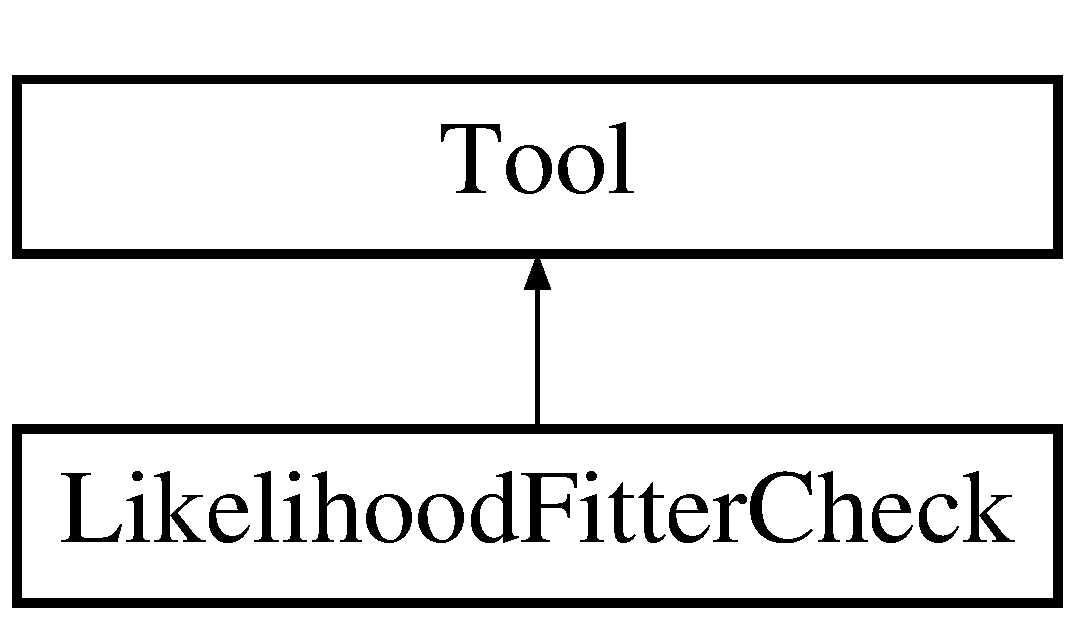
\includegraphics[height=2.000000cm]{classLikelihoodFitterCheck}
\end{center}
\end{figure}
\subsection*{Public Member Functions}
\begin{DoxyCompactItemize}
\item 
\hypertarget{classLikelihoodFitterCheck_a796e1357c908ddb2d16dd06d11daf199}{bool {\bfseries Initialise} (std\-::string configfile, \hyperlink{classDataModel}{Data\-Model} \&data)}\label{classLikelihoodFitterCheck_a796e1357c908ddb2d16dd06d11daf199}

\item 
bool \hyperlink{classLikelihoodFitterCheck_a7df99c1fac639db633877aeadde27ca7}{Execute} ()
\item 
\hypertarget{classLikelihoodFitterCheck_a4c454e19b497d56f47cd0d34632d5174}{bool {\bfseries Finalise} ()}\label{classLikelihoodFitterCheck_a4c454e19b497d56f47cd0d34632d5174}

\end{DoxyCompactItemize}


\subsection{Member Function Documentation}
\hypertarget{classLikelihoodFitterCheck_a7df99c1fac639db633877aeadde27ca7}{\index{Likelihood\-Fitter\-Check@{Likelihood\-Fitter\-Check}!Execute@{Execute}}
\index{Execute@{Execute}!LikelihoodFitterCheck@{Likelihood\-Fitter\-Check}}
\subsubsection[{Execute}]{\setlength{\rightskip}{0pt plus 5cm}bool Likelihood\-Fitter\-Check\-::\-Execute (
\begin{DoxyParamCaption}
{}
\end{DoxyParamCaption}
)}}\label{classLikelihoodFitterCheck_a7df99c1fac639db633877aeadde27ca7}
\begin{quotation}
Get digits from \char`\"{}\-Reco\-Event\char`\"{} \end{quotation}


\begin{quotation}
Get digits from \char`\"{}\-Reco\-Event\char`\"{} \end{quotation}


The documentation for this class was generated from the following files\-:\begin{DoxyCompactItemize}
\item 
User\-Tools/\-Likelihood\-Fitter\-Check/Likelihood\-Fitter\-Check.\-h\item 
User\-Tools/\-Likelihood\-Fitter\-Check/Likelihood\-Fitter\-Check.\-cpp\end{DoxyCompactItemize}

\hypertarget{classLoadANNIEEvent}{
\section{LoadANNIEEvent Class Reference}
\label{classLoadANNIEEvent}\index{LoadANNIEEvent@{LoadANNIEEvent}}
}
\subsection*{Public Member Functions}
\begin{DoxyCompactItemize}
\item 
\hypertarget{classLoadANNIEEvent_a273ac2b597344b138ff0142fa24bff06}{
bool {\bfseries Initialise} (std::string configfile, \hyperlink{classDataModel}{DataModel} \&data)}
\label{classLoadANNIEEvent_a273ac2b597344b138ff0142fa24bff06}

\item 
\hypertarget{classLoadANNIEEvent_af2c0686e7625d6a8ab5ebd692e78b182}{
bool {\bfseries Execute} ()}
\label{classLoadANNIEEvent_af2c0686e7625d6a8ab5ebd692e78b182}

\item 
\hypertarget{classLoadANNIEEvent_afcee0c0da54733f0c3dadb8c8879f494}{
bool {\bfseries Finalise} ()}
\label{classLoadANNIEEvent_afcee0c0da54733f0c3dadb8c8879f494}

\end{DoxyCompactItemize}
\subsection*{Protected Attributes}
\begin{DoxyCompactItemize}
\item 
\hypertarget{classLoadANNIEEvent_a1c9892604bb47cb58be2e7b6214ac773}{
int \hyperlink{classLoadANNIEEvent_a1c9892604bb47cb58be2e7b6214ac773}{verbosity\_\-}}
\label{classLoadANNIEEvent_a1c9892604bb47cb58be2e7b6214ac773}

\begin{DoxyCompactList}\small\item\em Integer code that determines the level of logging to show in the output. \item\end{DoxyCompactList}\item 
\hypertarget{classLoadANNIEEvent_a5de84624994fa2f83892fa7ad192c954}{
std::vector$<$ std::string $>$ \hyperlink{classLoadANNIEEvent_a5de84624994fa2f83892fa7ad192c954}{input\_\-filenames\_\-}}
\label{classLoadANNIEEvent_a5de84624994fa2f83892fa7ad192c954}

\begin{DoxyCompactList}\small\item\em Vector of filenames for each of the input files. \item\end{DoxyCompactList}\item 
\hypertarget{classLoadANNIEEvent_a9037abdb3ca42bcb45da4f76eaa5497f}{
size\_\-t \hyperlink{classLoadANNIEEvent_a9037abdb3ca42bcb45da4f76eaa5497f}{current\_\-entry\_\-}}
\label{classLoadANNIEEvent_a9037abdb3ca42bcb45da4f76eaa5497f}

\begin{DoxyCompactList}\small\item\em The index of the current entry in the ANNIEEvent store. \item\end{DoxyCompactList}\item 
\hypertarget{classLoadANNIEEvent_a92adda94f9be56cfb8a6507aa64d16f6}{
size\_\-t \hyperlink{classLoadANNIEEvent_a92adda94f9be56cfb8a6507aa64d16f6}{current\_\-file\_\-}}
\label{classLoadANNIEEvent_a92adda94f9be56cfb8a6507aa64d16f6}

\begin{DoxyCompactList}\small\item\em The index of the current file in this list of input files. \item\end{DoxyCompactList}\item 
\hypertarget{classLoadANNIEEvent_aabbd70eb8db780eb690f58cf76b7178e}{
size\_\-t \hyperlink{classLoadANNIEEvent_aabbd70eb8db780eb690f58cf76b7178e}{total\_\-entries\_\-in\_\-file\_\-}}
\label{classLoadANNIEEvent_aabbd70eb8db780eb690f58cf76b7178e}

\begin{DoxyCompactList}\small\item\em The total number of ANNIEEvent entries in the current file. \item\end{DoxyCompactList}\item 
\hypertarget{classLoadANNIEEvent_a276ac0416e1310830598036af7e2c0e3}{
bool \hyperlink{classLoadANNIEEvent_a276ac0416e1310830598036af7e2c0e3}{need\_\-new\_\-file\_\-}}
\label{classLoadANNIEEvent_a276ac0416e1310830598036af7e2c0e3}

\begin{DoxyCompactList}\small\item\em Flag indicating whether we need to load a new file. \item\end{DoxyCompactList}\item 
\hypertarget{classLoadANNIEEvent_a04316d23550d9c2f36f35f55ec054d20}{
std::stringstream {\bfseries logmessage}}
\label{classLoadANNIEEvent_a04316d23550d9c2f36f35f55ec054d20}

\end{DoxyCompactItemize}


The documentation for this class was generated from the following files:\begin{DoxyCompactItemize}
\item 
UserTools/LoadANNIEEvent/LoadANNIEEvent.h\item 
UserTools/LoadANNIEEvent/LoadANNIEEvent.cpp\end{DoxyCompactItemize}

\hypertarget{classLoadCCData}{\section{Load\-C\-C\-Data Class Reference}
\label{classLoadCCData}\index{Load\-C\-C\-Data@{Load\-C\-C\-Data}}
}
Inheritance diagram for Load\-C\-C\-Data\-:\begin{figure}[H]
\begin{center}
\leavevmode
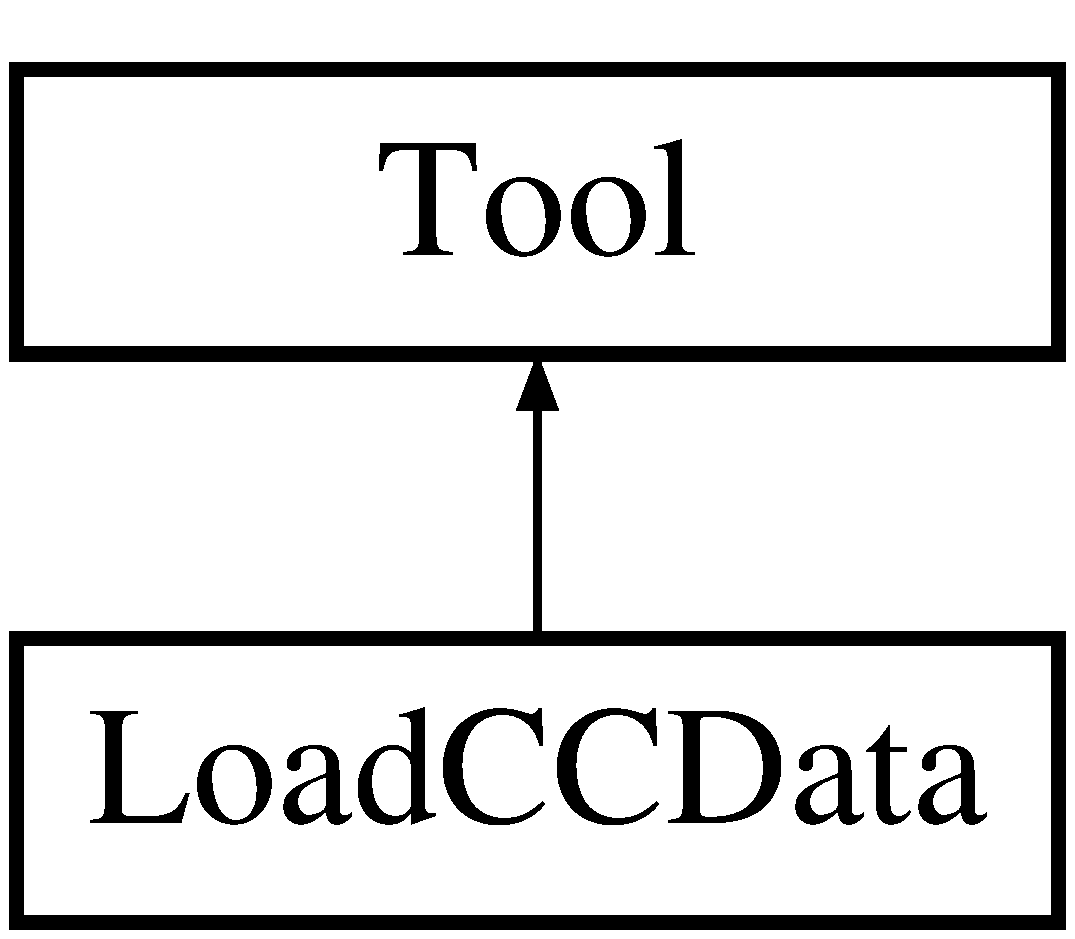
\includegraphics[height=2.000000cm]{classLoadCCData}
\end{center}
\end{figure}
\subsection*{Public Member Functions}
\begin{DoxyCompactItemize}
\item 
\hypertarget{classLoadCCData_ad27ea87d892f247f70f8b96ca67329b1}{bool {\bfseries Initialise} (std\-::string configfile, \hyperlink{classDataModel}{Data\-Model} \&data)}\label{classLoadCCData_ad27ea87d892f247f70f8b96ca67329b1}

\item 
\hypertarget{classLoadCCData_a102f586b9ad192e73b037c764dfd22e0}{bool {\bfseries Execute} ()}\label{classLoadCCData_a102f586b9ad192e73b037c764dfd22e0}

\item 
\hypertarget{classLoadCCData_adab5adee6f15c924a7077d63227e623c}{bool {\bfseries Finalise} ()}\label{classLoadCCData_adab5adee6f15c924a7077d63227e623c}

\end{DoxyCompactItemize}


The documentation for this class was generated from the following files\-:\begin{DoxyCompactItemize}
\item 
User\-Tools/\-Load\-C\-C\-Data/Load\-C\-C\-Data.\-h\item 
User\-Tools/\-Load\-C\-C\-Data/Load\-C\-C\-Data.\-cpp\end{DoxyCompactItemize}

\hypertarget{classLoadGeometry}{\section{Load\-Geometry Class Reference}
\label{classLoadGeometry}\index{Load\-Geometry@{Load\-Geometry}}
}
Inheritance diagram for Load\-Geometry\-:\begin{figure}[H]
\begin{center}
\leavevmode
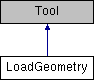
\includegraphics[height=2.000000cm]{classLoadGeometry}
\end{center}
\end{figure}
\subsection*{Public Member Functions}
\begin{DoxyCompactItemize}
\item 
\hypertarget{classLoadGeometry_aa1dfd5b2b31bc8dd32ec9c32d5a87f39}{bool {\bfseries Initialise} (std\-::string configfile, \hyperlink{classDataModel}{Data\-Model} \&data)}\label{classLoadGeometry_aa1dfd5b2b31bc8dd32ec9c32d5a87f39}

\item 
\hypertarget{classLoadGeometry_ad0b7de30c6142a5c1aa3ce5bb0f6adb5}{bool {\bfseries Execute} ()}\label{classLoadGeometry_ad0b7de30c6142a5c1aa3ce5bb0f6adb5}

\item 
\hypertarget{classLoadGeometry_ac13c3cfe39b857070143c37f8c0c74f3}{bool {\bfseries Finalise} ()}\label{classLoadGeometry_ac13c3cfe39b857070143c37f8c0c74f3}

\item 
\hypertarget{classLoadGeometry_a192b20dbff10b16767e60e6fc68dcdb1}{bool {\bfseries File\-Exists} (std\-::string name)}\label{classLoadGeometry_a192b20dbff10b16767e60e6fc68dcdb1}

\item 
\hypertarget{classLoadGeometry_a28fd063cca1f53e038320ea888fda636}{std\-::string {\bfseries Get\-Legend\-Line} (std\-::string name)}\label{classLoadGeometry_a28fd063cca1f53e038320ea888fda636}

\item 
\hypertarget{classLoadGeometry_a4303d74ac8cc0c015e73239beb170c44}{void {\bfseries Initialize\-Geometry} ()}\label{classLoadGeometry_a4303d74ac8cc0c015e73239beb170c44}

\item 
\hypertarget{classLoadGeometry_ab7fb2565b705f80e786b7cfa2f60dfc6}{void {\bfseries Load\-F\-A\-C\-C\-M\-R\-D\-Detectors} ()}\label{classLoadGeometry_ab7fb2565b705f80e786b7cfa2f60dfc6}

\item 
\hypertarget{classLoadGeometry_ac355939a78bda934e9efc64f3d801c95}{\hyperlink{classDetector}{Detector} {\bfseries Parse\-M\-R\-D\-Data\-Entry} (std\-::vector$<$ std\-::string $>$ Spec\-Line, std\-::vector$<$ std\-::string $>$ M\-R\-D\-Legend\-Entries)}\label{classLoadGeometry_ac355939a78bda934e9efc64f3d801c95}

\end{DoxyCompactItemize}
\subsection*{Public Attributes}
\begin{DoxyCompactItemize}
\item 
\hypertarget{classLoadGeometry_aaff5bd699a7b7d480adcdafde405360d}{\hyperlink{classGeometry}{Geometry} $\ast$ {\bfseries Annie\-Geometry}}\label{classLoadGeometry_aaff5bd699a7b7d480adcdafde405360d}

\end{DoxyCompactItemize}


The documentation for this class was generated from the following files\-:\begin{DoxyCompactItemize}
\item 
User\-Tools/\-Load\-Geometry/Load\-Geometry.\-h\item 
User\-Tools/\-Load\-Geometry/Load\-Geometry.\-cpp\end{DoxyCompactItemize}

\hypertarget{classLoadWCSim}{\section{Load\-W\-C\-Sim Class Reference}
\label{classLoadWCSim}\index{Load\-W\-C\-Sim@{Load\-W\-C\-Sim}}
}
Inheritance diagram for Load\-W\-C\-Sim\-:\begin{figure}[H]
\begin{center}
\leavevmode
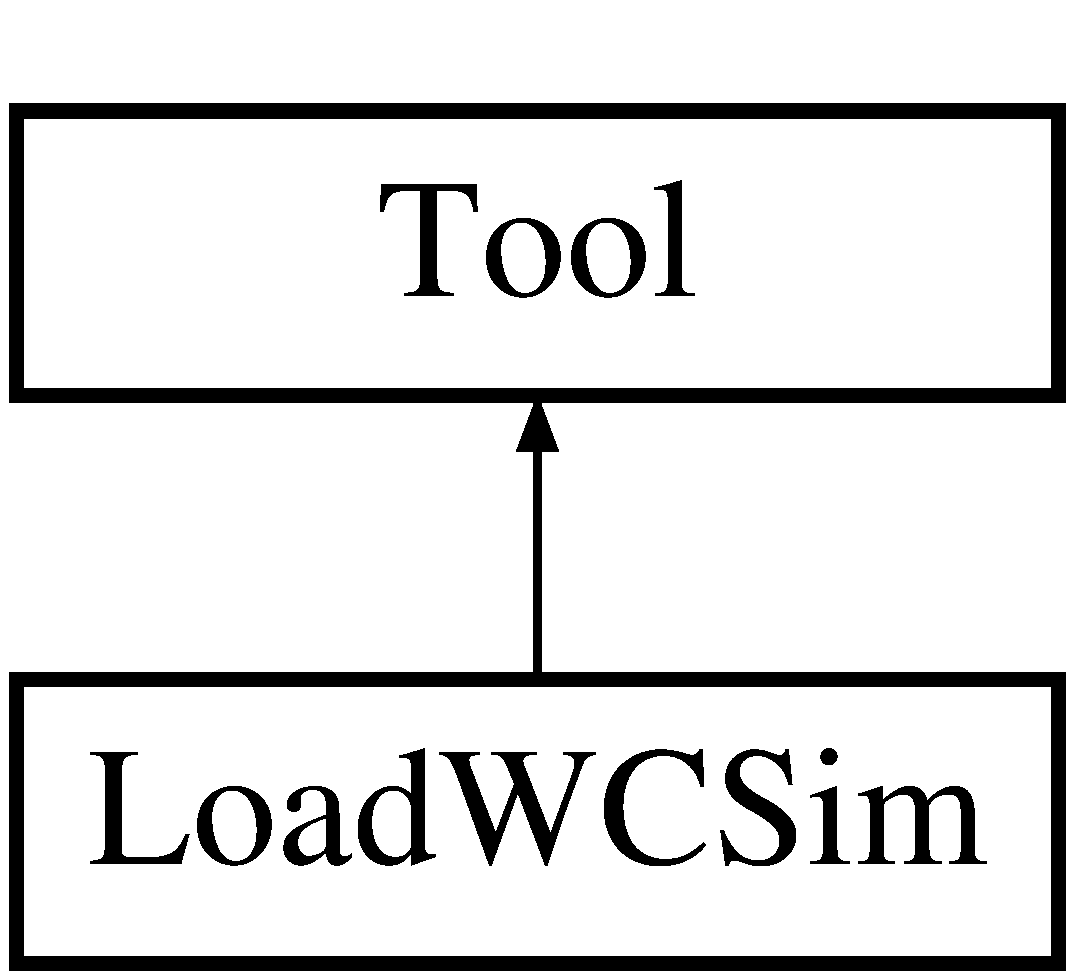
\includegraphics[height=2.000000cm]{classLoadWCSim}
\end{center}
\end{figure}
\subsection*{Public Member Functions}
\begin{DoxyCompactItemize}
\item 
\hypertarget{classLoadWCSim_a14c9d0f26dc099128ca670bd48b7cd34}{bool {\bfseries Initialise} (std\-::string configfile, \hyperlink{classDataModel}{Data\-Model} \&data)}\label{classLoadWCSim_a14c9d0f26dc099128ca670bd48b7cd34}

\item 
\hypertarget{classLoadWCSim_ae8b696ec0cbd3c0febee1c3482df3f7b}{bool {\bfseries Execute} ()}\label{classLoadWCSim_ae8b696ec0cbd3c0febee1c3482df3f7b}

\item 
\hypertarget{classLoadWCSim_afa581b87ca4db35eeb17bab6f40d169f}{bool {\bfseries Finalise} ()}\label{classLoadWCSim_afa581b87ca4db35eeb17bab6f40d169f}

\end{DoxyCompactItemize}


The documentation for this class was generated from the following files\-:\begin{DoxyCompactItemize}
\item 
User\-Tools/\-Load\-W\-C\-Sim/Load\-W\-C\-Sim.\-h\item 
User\-Tools/\-Load\-W\-C\-Sim/Load\-W\-C\-Sim.\-cpp\end{DoxyCompactItemize}

\hypertarget{classLoadWCSimLAPPD}{
\section{LoadWCSimLAPPD Class Reference}
\label{classLoadWCSimLAPPD}\index{LoadWCSimLAPPD@{LoadWCSimLAPPD}}
}
\subsection*{Public Member Functions}
\begin{DoxyCompactItemize}
\item 
\hypertarget{classLoadWCSimLAPPD_a1d2069798a83e0f34f41c4112b2343e8}{
bool {\bfseries Initialise} (std::string configfile, \hyperlink{classDataModel}{DataModel} \&data)}
\label{classLoadWCSimLAPPD_a1d2069798a83e0f34f41c4112b2343e8}

\item 
\hypertarget{classLoadWCSimLAPPD_a1b41167086f669fc1a71854a360406da}{
bool {\bfseries Execute} ()}
\label{classLoadWCSimLAPPD_a1b41167086f669fc1a71854a360406da}

\item 
\hypertarget{classLoadWCSimLAPPD_a457044289ecb5a3d18eeb6e8110a3902}{
bool {\bfseries Finalise} ()}
\label{classLoadWCSimLAPPD_a457044289ecb5a3d18eeb6e8110a3902}

\end{DoxyCompactItemize}


The documentation for this class was generated from the following files:\begin{DoxyCompactItemize}
\item 
UserTools/LoadWCSimLAPPD/LoadWCSimLAPPD.h\item 
UserTools/LoadWCSimLAPPD/LoadWCSimLAPPD.cpp\end{DoxyCompactItemize}

\hypertarget{classMCHit}{\section{M\-C\-Hit Class Reference}
\label{classMCHit}\index{M\-C\-Hit@{M\-C\-Hit}}
}
Inheritance diagram for M\-C\-Hit\-:\begin{figure}[H]
\begin{center}
\leavevmode
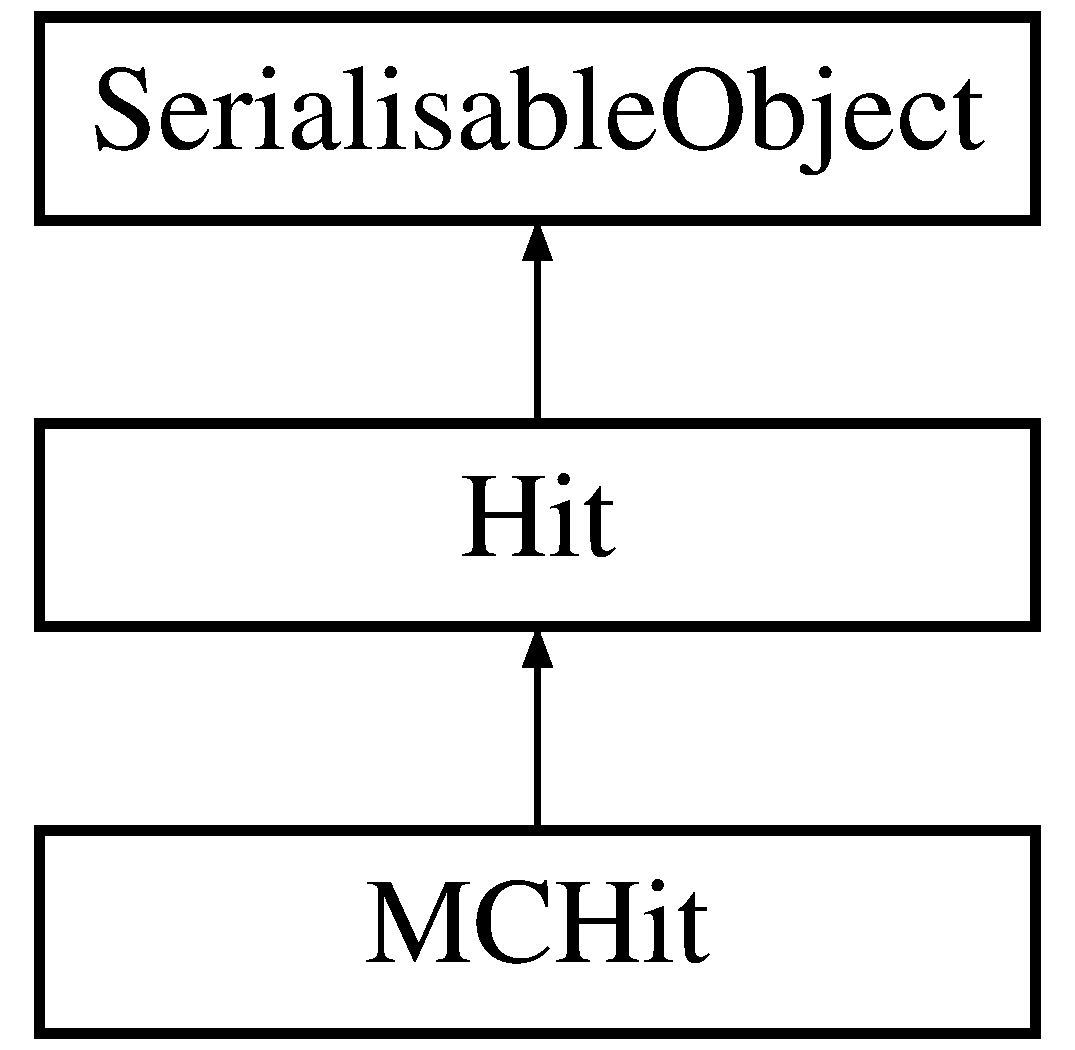
\includegraphics[height=3.000000cm]{classMCHit}
\end{center}
\end{figure}
\subsection*{Public Member Functions}
\begin{DoxyCompactItemize}
\item 
\hypertarget{classMCHit_aba6eea2703353998e3cdf5a23d388afc}{{\bfseries M\-C\-Hit} (int tubeid, double thetime, double thecharge, std\-::vector$<$ int $>$ theparents)}\label{classMCHit_aba6eea2703353998e3cdf5a23d388afc}

\item 
\hypertarget{classMCHit_af2a1f4ef53e27bd1c5962a1b61c784d0}{const std\-::vector$<$ int $>$ $\ast$ {\bfseries Get\-Parents} () const }\label{classMCHit_af2a1f4ef53e27bd1c5962a1b61c784d0}

\item 
\hypertarget{classMCHit_a18ae6be9fd39527f915e628ffe65dbec}{void {\bfseries Set\-Parents} (std\-::vector$<$ int $>$ parentsin)}\label{classMCHit_a18ae6be9fd39527f915e628ffe65dbec}

\item 
\hypertarget{classMCHit_a2d016ae3a18d9194a9a45a890f978833}{bool {\bfseries Print} ()}\label{classMCHit_a2d016ae3a18d9194a9a45a890f978833}

\end{DoxyCompactItemize}
\subsection*{Protected Member Functions}
\begin{DoxyCompactItemize}
\item 
\hypertarget{classMCHit_a8d516d5a6aeb3dd2f1b2e00b6532dcb5}{{\footnotesize template$<$class Archive $>$ }\\void {\bfseries serialize} (Archive \&ar, const unsigned int version)}\label{classMCHit_a8d516d5a6aeb3dd2f1b2e00b6532dcb5}

\end{DoxyCompactItemize}
\subsection*{Protected Attributes}
\begin{DoxyCompactItemize}
\item 
\hypertarget{classMCHit_a7fbd3892b201ed3790da046e63aed9d5}{std\-::vector$<$ int $>$ {\bfseries Parents}}\label{classMCHit_a7fbd3892b201ed3790da046e63aed9d5}

\end{DoxyCompactItemize}
\subsection*{Friends}
\begin{DoxyCompactItemize}
\item 
\hypertarget{classMCHit_ac98d07dd8f7b70e16ccb9a01abf56b9c}{class {\bfseries boost\-::serialization\-::access}}\label{classMCHit_ac98d07dd8f7b70e16ccb9a01abf56b9c}

\end{DoxyCompactItemize}


The documentation for this class was generated from the following file\-:\begin{DoxyCompactItemize}
\item 
Data\-Model/Hit.\-h\end{DoxyCompactItemize}

\include{classMCHitToHitComparer}
\hypertarget{classMCLAPPDHit}{
\section{MCLAPPDHit Class Reference}
\label{classMCLAPPDHit}\index{MCLAPPDHit@{MCLAPPDHit}}
}
Inheritance diagram for MCLAPPDHit::\begin{figure}[H]
\begin{center}
\leavevmode
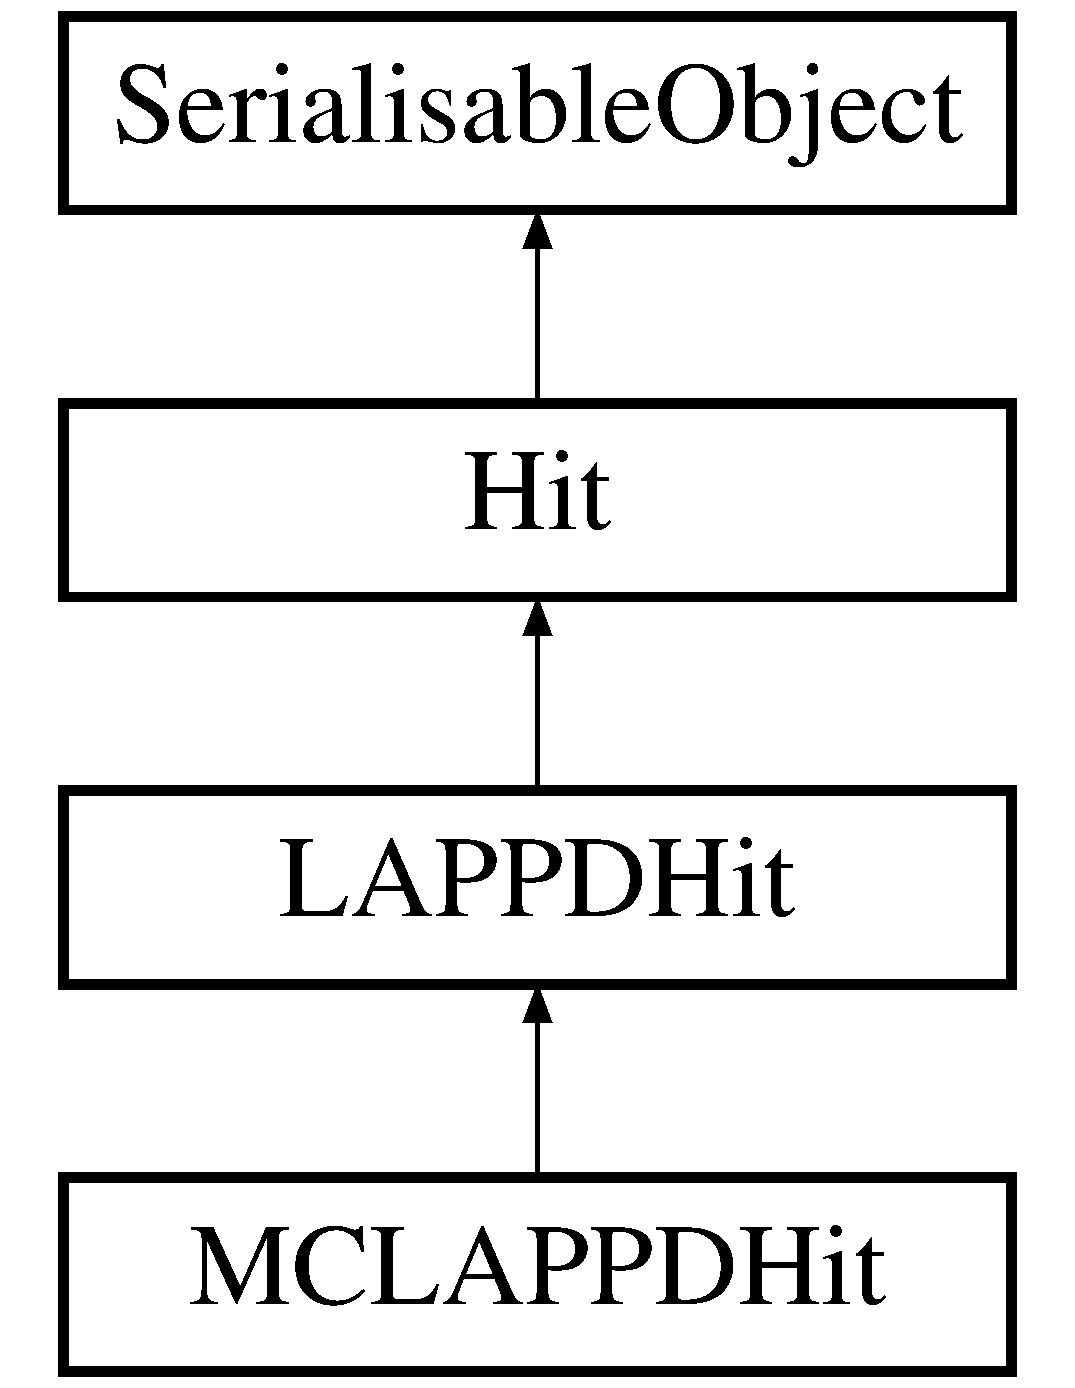
\includegraphics[height=4cm]{classMCLAPPDHit}
\end{center}
\end{figure}
\subsection*{Public Member Functions}
\begin{DoxyCompactItemize}
\item 
\hypertarget{classMCLAPPDHit_a376553aaa3ca2a5920e04fbb116a0b55}{
{\bfseries Parents} (theparents)}
\label{classMCLAPPDHit_a376553aaa3ca2a5920e04fbb116a0b55}

\item 
\hypertarget{classMCLAPPDHit_a2cd53e715b43962eece869e296f0efdb}{
const std::vector$<$ int $>$ $\ast$ {\bfseries GetParents} () const }
\label{classMCLAPPDHit_a2cd53e715b43962eece869e296f0efdb}

\item 
\hypertarget{classMCLAPPDHit_a1edf49747c6858e203a3185ec0f656a4}{
void {\bfseries SetParents} (std::vector$<$ int $>$ parentsin)}
\label{classMCLAPPDHit_a1edf49747c6858e203a3185ec0f656a4}

\item 
\hypertarget{classMCLAPPDHit_a90639fe126043eeb4222860265d0e3c5}{
bool {\bfseries Print} ()}
\label{classMCLAPPDHit_a90639fe126043eeb4222860265d0e3c5}

\item 
\hypertarget{classMCLAPPDHit_ad04838bfc8db66fff91d0bd8f5ff48b5}{
{\footnotesize template$<$class Archive $>$ }\\void {\bfseries serialize} (Archive \&ar, const unsigned int version)}
\label{classMCLAPPDHit_ad04838bfc8db66fff91d0bd8f5ff48b5}

\end{DoxyCompactItemize}
\subsection*{Protected Attributes}
\begin{DoxyCompactItemize}
\item 
\hypertarget{classMCLAPPDHit_af7f2b72e3e33a3037b5a23b3441c7ce5}{
std::vector$<$ int $>$ {\bfseries Parents}}
\label{classMCLAPPDHit_af7f2b72e3e33a3037b5a23b3441c7ce5}

\end{DoxyCompactItemize}
\subsection*{Friends}
\begin{DoxyCompactItemize}
\item 
\hypertarget{classMCLAPPDHit_ac98d07dd8f7b70e16ccb9a01abf56b9c}{
class {\bfseries boost::serialization::access}}
\label{classMCLAPPDHit_ac98d07dd8f7b70e16ccb9a01abf56b9c}

\end{DoxyCompactItemize}


The documentation for this class was generated from the following file:\begin{DoxyCompactItemize}
\item 
DataModel/LAPPDHit.h\end{DoxyCompactItemize}

\hypertarget{classMCParticle}{\section{M\-C\-Particle Class Reference}
\label{classMCParticle}\index{M\-C\-Particle@{M\-C\-Particle}}
}
Inheritance diagram for M\-C\-Particle\-:\begin{figure}[H]
\begin{center}
\leavevmode
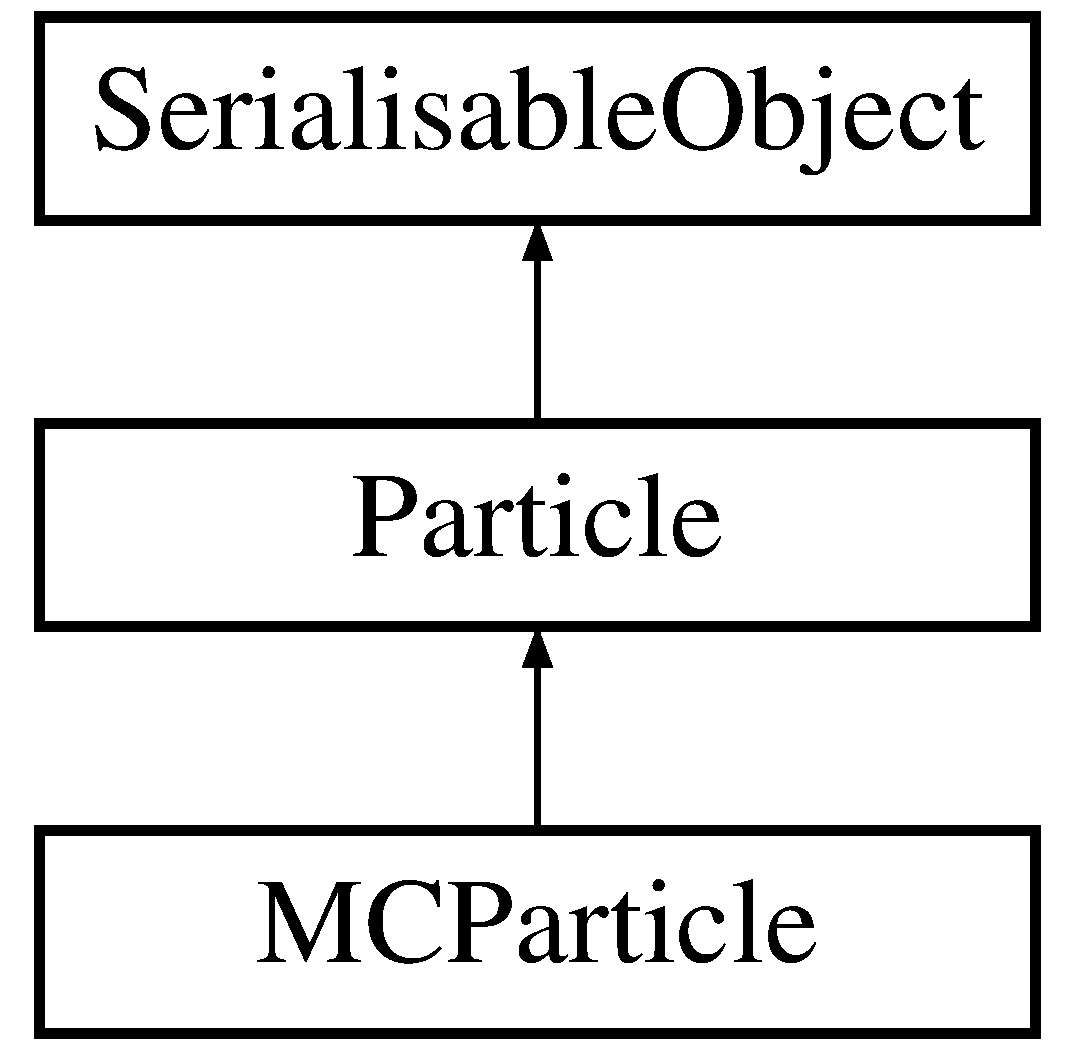
\includegraphics[height=3.000000cm]{classMCParticle}
\end{center}
\end{figure}
\subsection*{Public Member Functions}
\begin{DoxyCompactItemize}
\item 
\hypertarget{classMCParticle_a1e2054a5aa6978bec68fa15133e9aae9}{{\bfseries M\-C\-Particle} (int pdg, double stt\-E, double stp\-E, \hyperlink{classPosition}{Position} sttpos, \hyperlink{classPosition}{Position} stppos, double sttt, double stpt, \hyperlink{classDirection}{Direction} startdir, double len, tracktype tracktypein, int partid, int parentpdg, int flagid)}\label{classMCParticle_a1e2054a5aa6978bec68fa15133e9aae9}

\item 
\hypertarget{classMCParticle_a351d384bc2af0918ece85ba38c9551b2}{int {\bfseries Get\-Particle\-I\-D} ()}\label{classMCParticle_a351d384bc2af0918ece85ba38c9551b2}

\item 
\hypertarget{classMCParticle_a05c2ded23b19858448647ce9d2ba36fd}{int {\bfseries Get\-Parent\-Pdg} ()}\label{classMCParticle_a05c2ded23b19858448647ce9d2ba36fd}

\item 
\hypertarget{classMCParticle_a3240caaaac37a2d4ab3ef5d57aa53e74}{int {\bfseries Get\-Flag} ()}\label{classMCParticle_a3240caaaac37a2d4ab3ef5d57aa53e74}

\item 
\hypertarget{classMCParticle_a1829807b49dda47903441234983df064}{bool {\bfseries Get\-Starts\-In\-Fiducial\-Volume} ()}\label{classMCParticle_a1829807b49dda47903441234983df064}

\item 
\hypertarget{classMCParticle_a99c79b20440359ee841296eff1a4ab61}{double {\bfseries Get\-Track\-Angle\-X} ()}\label{classMCParticle_a99c79b20440359ee841296eff1a4ab61}

\item 
\hypertarget{classMCParticle_a98e706fd77669b0461e739b5a8e46998}{double {\bfseries Get\-Track\-Angle\-Y} ()}\label{classMCParticle_a98e706fd77669b0461e739b5a8e46998}

\item 
\hypertarget{classMCParticle_ae5bbdd4456fb3131ec6eb7213cab54cb}{double {\bfseries Get\-Track\-Angle\-From\-Beam} ()}\label{classMCParticle_ae5bbdd4456fb3131ec6eb7213cab54cb}

\item 
\hypertarget{classMCParticle_aa9626a1846b63292b5356fe2be097fe9}{bool {\bfseries Get\-Enters\-Tank} ()}\label{classMCParticle_aa9626a1846b63292b5356fe2be097fe9}

\item 
\hypertarget{classMCParticle_a112df02772c9bc084298a54b86212133}{\hyperlink{classPosition}{Position} {\bfseries Get\-Tank\-Entry\-Point} ()}\label{classMCParticle_a112df02772c9bc084298a54b86212133}

\item 
\hypertarget{classMCParticle_a6a7562aabf349e90c0e1e3751189e5eb}{bool {\bfseries Get\-Exits\-Tank} ()}\label{classMCParticle_a6a7562aabf349e90c0e1e3751189e5eb}

\item 
\hypertarget{classMCParticle_a6693f8f91b1ecab9309ffb752f5fcd66}{\hyperlink{classPosition}{Position} {\bfseries Get\-Tank\-Exit\-Point} ()}\label{classMCParticle_a6693f8f91b1ecab9309ffb752f5fcd66}

\item 
\hypertarget{classMCParticle_a9137f3783a143643ef16b3b63fdabef8}{double {\bfseries Get\-Track\-Length\-In\-Tank} ()}\label{classMCParticle_a9137f3783a143643ef16b3b63fdabef8}

\item 
\hypertarget{classMCParticle_a6b69dd58bc549a57cc780a9621c8fcad}{bool {\bfseries Get\-Enters\-Mrd} ()}\label{classMCParticle_a6b69dd58bc549a57cc780a9621c8fcad}

\item 
\hypertarget{classMCParticle_a4fc1d825ca0b6898323718e382574df0}{\hyperlink{classPosition}{Position} {\bfseries Get\-Mrd\-Entry\-Point} ()}\label{classMCParticle_a4fc1d825ca0b6898323718e382574df0}

\item 
\hypertarget{classMCParticle_a5f529c1629fdaf94d6061d1bde2013bc}{bool {\bfseries Get\-Exits\-Mrd} ()}\label{classMCParticle_a5f529c1629fdaf94d6061d1bde2013bc}

\item 
\hypertarget{classMCParticle_a33f74539498e327f17345f5801b9ce60}{\hyperlink{classPosition}{Position} {\bfseries Get\-Mrd\-Exit\-Point} ()}\label{classMCParticle_a33f74539498e327f17345f5801b9ce60}

\item 
\hypertarget{classMCParticle_ab4172cbc5024701f1286ec9b3cdae9a7}{bool {\bfseries Get\-Penetrates\-Mrd} ()}\label{classMCParticle_ab4172cbc5024701f1286ec9b3cdae9a7}

\item 
\hypertarget{classMCParticle_a46bf3f4fb48252b4f459b77b108a8e67}{double {\bfseries Get\-Track\-Length\-In\-Mrd} ()}\label{classMCParticle_a46bf3f4fb48252b4f459b77b108a8e67}

\item 
\hypertarget{classMCParticle_a3d260af122ff90824de2e2be7f672f07}{double {\bfseries Get\-Mrd\-Penetration} ()}\label{classMCParticle_a3d260af122ff90824de2e2be7f672f07}

\item 
\hypertarget{classMCParticle_afa08a1cb74a4b0b642f0b62c04114976}{int {\bfseries Get\-Num\-Mrd\-Layers\-Penetrated} ()}\label{classMCParticle_afa08a1cb74a4b0b642f0b62c04114976}

\item 
\hypertarget{classMCParticle_ac8325eb8dd7e2d10b6b406dfcd6b31af}{double {\bfseries Get\-Mrd\-Energy\-Loss} ()}\label{classMCParticle_ac8325eb8dd7e2d10b6b406dfcd6b31af}

\item 
\hypertarget{classMCParticle_ab3f8776c846fcc1c82f2d9083beaf07f}{void {\bfseries Set\-Particle\-I\-D} (int partidin)}\label{classMCParticle_ab3f8776c846fcc1c82f2d9083beaf07f}

\item 
\hypertarget{classMCParticle_a835ce089d630c4624a3060980450ca2c}{void {\bfseries Set\-Parent\-Pdg} (int parentpdgin)}\label{classMCParticle_a835ce089d630c4624a3060980450ca2c}

\item 
\hypertarget{classMCParticle_ace8eaad4c1fd7398fb5bda3316b5395b}{void {\bfseries Set\-Flag} (int flagidin)}\label{classMCParticle_ace8eaad4c1fd7398fb5bda3316b5395b}

\item 
\hypertarget{classMCParticle_a2a42a4f6ef9af8a6158e422680a57b47}{void {\bfseries Set\-Starts\-In\-Fiducial\-Volume} (bool i\-Starts\-In\-Fiducial\-Volume)}\label{classMCParticle_a2a42a4f6ef9af8a6158e422680a57b47}

\item 
\hypertarget{classMCParticle_a1fb1b9c4206de10c602b1095e6428578}{void {\bfseries Set\-Enters\-Tank} (bool i\-Enters\-Tank)}\label{classMCParticle_a1fb1b9c4206de10c602b1095e6428578}

\item 
\hypertarget{classMCParticle_a2cfded14729766192df1b9770edba92a}{void {\bfseries Set\-Tank\-Entry\-Point} (\hyperlink{classPosition}{Position} i\-Tank\-Entry\-Point)}\label{classMCParticle_a2cfded14729766192df1b9770edba92a}

\item 
\hypertarget{classMCParticle_a702069712afdc032362de66c133c0165}{void {\bfseries Set\-Exits\-Tank} (bool i\-Exits\-Tank)}\label{classMCParticle_a702069712afdc032362de66c133c0165}

\item 
\hypertarget{classMCParticle_a1cbf3a6c05ac82ec5e9c8b90a70c2940}{void {\bfseries Set\-Tank\-Exit\-Point} (\hyperlink{classPosition}{Position} i\-Tank\-Exit\-Point)}\label{classMCParticle_a1cbf3a6c05ac82ec5e9c8b90a70c2940}

\item 
\hypertarget{classMCParticle_a7ca9800559d1e4fddd3fc98c0deb2c99}{void {\bfseries Set\-Track\-Length\-In\-Tank} (double i\-Track\-Length\-In\-Tank)}\label{classMCParticle_a7ca9800559d1e4fddd3fc98c0deb2c99}

\item 
\hypertarget{classMCParticle_a0538d9cb8cf49a824f3fd77d0531e935}{void {\bfseries Set\-Enters\-Mrd} (bool i\-Enters\-Mrd)}\label{classMCParticle_a0538d9cb8cf49a824f3fd77d0531e935}

\item 
\hypertarget{classMCParticle_a5ac43b6d4e343123b0308aeff287a1ec}{void {\bfseries Set\-Mrd\-Entry\-Point} (\hyperlink{classPosition}{Position} i\-Mrd\-Entry\-Point)}\label{classMCParticle_a5ac43b6d4e343123b0308aeff287a1ec}

\item 
\hypertarget{classMCParticle_ad11395d2bd739fc1ad5d473f6313a34a}{void {\bfseries Set\-Exits\-Mrd} (bool i\-Exits\-Mrd)}\label{classMCParticle_ad11395d2bd739fc1ad5d473f6313a34a}

\item 
\hypertarget{classMCParticle_a775d17a50fd84cd07f9049aff86f0ead}{void {\bfseries Set\-Mrd\-Exit\-Point} (\hyperlink{classPosition}{Position} i\-Mrd\-Exit\-Point)}\label{classMCParticle_a775d17a50fd84cd07f9049aff86f0ead}

\item 
\hypertarget{classMCParticle_ab112ca1f301435bb933ba813d7a4da3e}{void {\bfseries Set\-Penetrates\-Mrd} (bool i\-Penetrates\-Mrd)}\label{classMCParticle_ab112ca1f301435bb933ba813d7a4da3e}

\item 
\hypertarget{classMCParticle_af85b13f2164e52e752d6e14534d4b31c}{void {\bfseries Set\-Track\-Length\-In\-Mrd} (double i\-Track\-Length\-In\-Mrd)}\label{classMCParticle_af85b13f2164e52e752d6e14534d4b31c}

\item 
\hypertarget{classMCParticle_a1bd0d632655c48ee8bc311b7ab9c3996}{void {\bfseries Set\-Mrd\-Penetration} (double i\-Mrd\-Penetration)}\label{classMCParticle_a1bd0d632655c48ee8bc311b7ab9c3996}

\item 
\hypertarget{classMCParticle_abc4ac222c79d03dd421dccf1c27aa461}{void {\bfseries Set\-Num\-Mrd\-Layers\-Penetrated} (int i\-Mrd\-Layers\-Penetrated)}\label{classMCParticle_abc4ac222c79d03dd421dccf1c27aa461}

\item 
\hypertarget{classMCParticle_a3db0d00c918e435c4cacc51e80fad7db}{void {\bfseries Set\-Mrd\-Energy\-Loss} (double i\-Mrd\-Energy\-Loss)}\label{classMCParticle_a3db0d00c918e435c4cacc51e80fad7db}

\item 
\hypertarget{classMCParticle_abc9a006d2fb4c95ca7f08fa218867c21}{void {\bfseries Set\-Track\-Angle\-X} (double i\-Track\-Angle\-X)}\label{classMCParticle_abc9a006d2fb4c95ca7f08fa218867c21}

\item 
\hypertarget{classMCParticle_af39b59b0cde215f2a6fe2183d8c580b9}{void {\bfseries Set\-Track\-Angle\-Y} (double i\-Track\-Angle\-Y)}\label{classMCParticle_af39b59b0cde215f2a6fe2183d8c580b9}

\item 
\hypertarget{classMCParticle_af278f6d766d7a4cc4818ae0b3e64f73f}{void {\bfseries Set\-Track\-Angle\-From\-Beam} (double i\-Track\-Angle\-From\-Beam)}\label{classMCParticle_af278f6d766d7a4cc4818ae0b3e64f73f}

\item 
\hypertarget{classMCParticle_a1691c5d5d847e0a2419cdad793ff2ddb}{bool {\bfseries Get\-World\-Contained} (int startstop, \hyperlink{classPosition}{Position} a\-Vertex=\hyperlink{classPosition}{Position}(0, 0, 0))}\label{classMCParticle_a1691c5d5d847e0a2419cdad793ff2ddb}

\item 
\hypertarget{classMCParticle_a602114887228de2afbfcd0a31ddba66c}{bool {\bfseries Print} ()}\label{classMCParticle_a602114887228de2afbfcd0a31ddba66c}

\end{DoxyCompactItemize}
\subsection*{Protected Member Functions}
\begin{DoxyCompactItemize}
\item 
\hypertarget{classMCParticle_ac28878d706363533ac74f18faf272fb4}{{\footnotesize template$<$class Archive $>$ }\\void {\bfseries serialize} (Archive \&ar, const unsigned int version)}\label{classMCParticle_ac28878d706363533ac74f18faf272fb4}

\end{DoxyCompactItemize}
\subsection*{Protected Attributes}
\begin{DoxyCompactItemize}
\item 
\hypertarget{classMCParticle_a52ca5b486dd9ded3b7da2b77c2704f85}{int {\bfseries Particle\-I\-D}}\label{classMCParticle_a52ca5b486dd9ded3b7da2b77c2704f85}

\item 
\hypertarget{classMCParticle_aa60d9c88e4c168be89a8075414078e82}{int {\bfseries Parent\-Pdg}}\label{classMCParticle_aa60d9c88e4c168be89a8075414078e82}

\item 
\hypertarget{classMCParticle_a74ff96a2e3f2c92d991a631dc320b343}{int {\bfseries Flag}}\label{classMCParticle_a74ff96a2e3f2c92d991a631dc320b343}

\item 
\hypertarget{classMCParticle_a9328c826d1ee1d615e312d25235d04a0}{bool {\bfseries Starts\-In\-Fiducial\-Volume}}\label{classMCParticle_a9328c826d1ee1d615e312d25235d04a0}

\item 
\hypertarget{classMCParticle_aafb0416bfa7dfcaa14f4243d76930239}{double {\bfseries Track\-Angle\-X}}\label{classMCParticle_aafb0416bfa7dfcaa14f4243d76930239}

\item 
\hypertarget{classMCParticle_aaf4a5cd3469f3d527c0ac8f4e3713c4b}{double {\bfseries Track\-Angle\-Y}}\label{classMCParticle_aaf4a5cd3469f3d527c0ac8f4e3713c4b}

\item 
\hypertarget{classMCParticle_af4cdfb96769ec1a40e45c4f40b9eb520}{double {\bfseries Track\-Angle\-From\-Beam}}\label{classMCParticle_af4cdfb96769ec1a40e45c4f40b9eb520}

\item 
\hypertarget{classMCParticle_afc38d81f454f0011d513db8dedc39d37}{bool {\bfseries Enters\-Tank}}\label{classMCParticle_afc38d81f454f0011d513db8dedc39d37}

\item 
\hypertarget{classMCParticle_ad1c64ca6b80955ea88cc1014360c53fa}{\hyperlink{classPosition}{Position} {\bfseries Tank\-Entry\-Point}}\label{classMCParticle_ad1c64ca6b80955ea88cc1014360c53fa}

\item 
\hypertarget{classMCParticle_aa33826267b580a0e0083df6deaeb26ce}{bool {\bfseries Exits\-Tank}}\label{classMCParticle_aa33826267b580a0e0083df6deaeb26ce}

\item 
\hypertarget{classMCParticle_a9d57e7bfd963f6ee5cdf4de16b15652f}{\hyperlink{classPosition}{Position} {\bfseries Tank\-Exit\-Point}}\label{classMCParticle_a9d57e7bfd963f6ee5cdf4de16b15652f}

\item 
\hypertarget{classMCParticle_a3a178c1eab5c3e1baca3d7416066cff5}{double {\bfseries Track\-Length\-In\-Tank}}\label{classMCParticle_a3a178c1eab5c3e1baca3d7416066cff5}

\item 
\hypertarget{classMCParticle_aca01ce3d68f3eb4fa1aea0e052da2322}{double {\bfseries Enters\-Mrd}}\label{classMCParticle_aca01ce3d68f3eb4fa1aea0e052da2322}

\item 
\hypertarget{classMCParticle_a06f90a30827626e16ce036b725032424}{\hyperlink{classPosition}{Position} {\bfseries Mrd\-Entry\-Point}}\label{classMCParticle_a06f90a30827626e16ce036b725032424}

\item 
\hypertarget{classMCParticle_ac2690fd0362dcad58682cda54179035c}{bool {\bfseries Exits\-Mrd}}\label{classMCParticle_ac2690fd0362dcad58682cda54179035c}

\item 
\hypertarget{classMCParticle_a79fe95c4ab5a161f31f42809dda35d8e}{\hyperlink{classPosition}{Position} {\bfseries Mrd\-Exit\-Point}}\label{classMCParticle_a79fe95c4ab5a161f31f42809dda35d8e}

\item 
\hypertarget{classMCParticle_ad82f8f04628606c79b789cdaad72c73d}{bool {\bfseries Penetrates\-Mrd}}\label{classMCParticle_ad82f8f04628606c79b789cdaad72c73d}

\item 
\hypertarget{classMCParticle_affee0c98fd66da0ce6c704fee413b120}{double {\bfseries Track\-Length\-In\-Mrd}}\label{classMCParticle_affee0c98fd66da0ce6c704fee413b120}

\item 
\hypertarget{classMCParticle_aae98f51a041e389e7439cfe2229e1936}{double {\bfseries Mrd\-Penetration}}\label{classMCParticle_aae98f51a041e389e7439cfe2229e1936}

\item 
\hypertarget{classMCParticle_ae3e7da6821154bc8a5817e87ec10b6ea}{int {\bfseries Mrd\-Layers\-Penetrated}}\label{classMCParticle_ae3e7da6821154bc8a5817e87ec10b6ea}

\item 
\hypertarget{classMCParticle_a4c8a5b9e7d2f4268fa4a60e5d80dcc22}{double {\bfseries Mrd\-Energy\-Loss}}\label{classMCParticle_a4c8a5b9e7d2f4268fa4a60e5d80dcc22}

\end{DoxyCompactItemize}
\subsection*{Friends}
\begin{DoxyCompactItemize}
\item 
\hypertarget{classMCParticle_ac98d07dd8f7b70e16ccb9a01abf56b9c}{class {\bfseries boost\-::serialization\-::access}}\label{classMCParticle_ac98d07dd8f7b70e16ccb9a01abf56b9c}

\end{DoxyCompactItemize}
\subsection*{Additional Inherited Members}


The documentation for this class was generated from the following file\-:\begin{DoxyCompactItemize}
\item 
Data\-Model/Particle.\-h\end{DoxyCompactItemize}

\hypertarget{classMCParticleProperties}{
\section{MCParticleProperties Class Reference}
\label{classMCParticleProperties}\index{MCParticleProperties@{MCParticleProperties}}
}
\subsection*{Public Member Functions}
\begin{DoxyCompactItemize}
\item 
\hypertarget{classMCParticleProperties_aeb42d506b628e71bad8d15c6d20b7728}{
bool {\bfseries Initialise} (std::string configfile, \hyperlink{classDataModel}{DataModel} \&data)}
\label{classMCParticleProperties_aeb42d506b628e71bad8d15c6d20b7728}

\item 
\hypertarget{classMCParticleProperties_a93cf4884b81b864d9a40ae53689ad9f8}{
bool {\bfseries Execute} ()}
\label{classMCParticleProperties_a93cf4884b81b864d9a40ae53689ad9f8}

\item 
\hypertarget{classMCParticleProperties_a6ed9e609a5194be6d1c2461759b086f1}{
bool {\bfseries Finalise} ()}
\label{classMCParticleProperties_a6ed9e609a5194be6d1c2461759b086f1}

\end{DoxyCompactItemize}


The documentation for this class was generated from the following files:\begin{DoxyCompactItemize}
\item 
UserTools/MCParticleProperties/MCParticleProperties.h\item 
UserTools/MCParticleProperties/MCParticleProperties.cpp\end{DoxyCompactItemize}

\hypertarget{classMCRecoEventLoader}{
\section{MCRecoEventLoader Class Reference}
\label{classMCRecoEventLoader}\index{MCRecoEventLoader@{MCRecoEventLoader}}
}
\subsection*{Public Member Functions}
\begin{DoxyCompactItemize}
\item 
bool \hyperlink{classMCRecoEventLoader_a3c57d089982246d613d553092ab8f141}{Initialise} (std::string configfile, \hyperlink{classDataModel}{DataModel} \&data)
\item 
bool \hyperlink{classMCRecoEventLoader_a17027f8a3689b459fa54a4a3c84b5a0c}{Execute} ()
\item 
\hypertarget{classMCRecoEventLoader_ac4b21a91ed4795b7ffc9695ec38438e2}{
bool {\bfseries Finalise} ()}
\label{classMCRecoEventLoader_ac4b21a91ed4795b7ffc9695ec38438e2}

\item 
void \hyperlink{classMCRecoEventLoader_a981fbf41206f4be37c40ec5fbaeb9c9d}{FindTrueVertexFromMC} ()
\begin{DoxyCompactList}\small\item\em Find true neutrino vertex. \item\end{DoxyCompactList}\item 
void \hyperlink{classMCRecoEventLoader_ade2e70b075295f19384e6862dda123ec}{FindPionKaonCountFromMC} ()
\begin{DoxyCompactList}\small\item\em Find PionKaon Count. \item\end{DoxyCompactList}\item 
void \hyperlink{classMCRecoEventLoader_a4d3d3f6e9b15bd07420b0b10f04eed11}{PushTrueVertex} (bool savetodisk)
\begin{DoxyCompactList}\small\item\em Save true neutrino vertex. \item\end{DoxyCompactList}\item 
void \hyperlink{classMCRecoEventLoader_a57ec5fa238eed8885465bf6d3e03078c}{PushTrueStopVertex} (bool savetodisk)
\begin{DoxyCompactList}\small\item\em Save true neutrino vertex. \item\end{DoxyCompactList}\item 
void \hyperlink{classMCRecoEventLoader_a253c2747d42e4112c039ecafc93ee05e}{PushTrueMuonEnergy} (double MuE)
\begin{DoxyCompactList}\small\item\em Push muon track lengths to RecoEvent Store. \item\end{DoxyCompactList}\item 
void \hyperlink{classMCRecoEventLoader_a79a348512d9c7fb13aa86e96d5f1d39b}{PushTrueWaterTrackLength} (double WaterT)
\item 
void \hyperlink{classMCRecoEventLoader_a258d351d5afce9a2be153db10a80ae3a}{PushTrueMRDTrackLength} (double MRDT)
\item 
void \hyperlink{classMCRecoEventLoader_a1c01acb2c109e46de4e1dc27911843c3}{Reset} ()
\begin{DoxyCompactList}\small\item\em Reset initialized classes. \item\end{DoxyCompactList}\end{DoxyCompactItemize}
\subsection*{Public Attributes}
\begin{DoxyCompactItemize}
\item 
\hypertarget{classMCRecoEventLoader_a42b09a53c17f03a6e4fcce20cd4c56b1}{
int {\bfseries verbosity} = 1}
\label{classMCRecoEventLoader_a42b09a53c17f03a6e4fcce20cd4c56b1}

\item 
\hypertarget{classMCRecoEventLoader_a0d3eb072ae7301282ba510bbd11ffb0d}{
bool {\bfseries fGetPiKInfo}}
\label{classMCRecoEventLoader_a0d3eb072ae7301282ba510bbd11ffb0d}

\item 
\hypertarget{classMCRecoEventLoader_ab936432f202a835b7877dbc63303a57c}{
int {\bfseries fParticleID}}
\label{classMCRecoEventLoader_ab936432f202a835b7877dbc63303a57c}

\item 
\hypertarget{classMCRecoEventLoader_aefded74813d943854628aa0da13953ff}{
double {\bfseries xshift}}
\label{classMCRecoEventLoader_aefded74813d943854628aa0da13953ff}

\item 
\hypertarget{classMCRecoEventLoader_a008cd13186e5458c4232376980ff8430}{
double {\bfseries yshift}}
\label{classMCRecoEventLoader_a008cd13186e5458c4232376980ff8430}

\item 
\hypertarget{classMCRecoEventLoader_a5320937dd08d67c172b0f90956615e11}{
double {\bfseries zshift}}
\label{classMCRecoEventLoader_a5320937dd08d67c172b0f90956615e11}

\item 
\hypertarget{classMCRecoEventLoader_a06c8c257c06cca00a6b34c51365e6d69}{
\hyperlink{classRecoVertex}{RecoVertex} $\ast$ \hyperlink{classMCRecoEventLoader_a06c8c257c06cca00a6b34c51365e6d69}{fMuonStartVertex} = nullptr}
\label{classMCRecoEventLoader_a06c8c257c06cca00a6b34c51365e6d69}

\begin{DoxyCompactList}\small\item\em true muon start vertex \item\end{DoxyCompactList}\item 
\hypertarget{classMCRecoEventLoader_ab4eb6938d73f33b4d4fbcaccd28f9c65}{
\hyperlink{classRecoVertex}{RecoVertex} $\ast$ \hyperlink{classMCRecoEventLoader_ab4eb6938d73f33b4d4fbcaccd28f9c65}{fMuonStopVertex} = nullptr}
\label{classMCRecoEventLoader_ab4eb6938d73f33b4d4fbcaccd28f9c65}

\begin{DoxyCompactList}\small\item\em true muon stop vertex \item\end{DoxyCompactList}\item 
\hypertarget{classMCRecoEventLoader_a92922e07f398c491b9fd9e13ef012689}{
std::vector$<$ \hyperlink{classMCParticle}{MCParticle} $>$ $\ast$ \hyperlink{classMCRecoEventLoader_a92922e07f398c491b9fd9e13ef012689}{fMCParticles} = nullptr}
\label{classMCRecoEventLoader_a92922e07f398c491b9fd9e13ef012689}

\begin{DoxyCompactList}\small\item\em truth tracks \item\end{DoxyCompactList}\item 
\hypertarget{classMCRecoEventLoader_a6f1746151a4cc1c80204de806e6d3086}{
double {\bfseries TrueMuonEnergy} = -\/9999.}
\label{classMCRecoEventLoader_a6f1746151a4cc1c80204de806e6d3086}

\item 
\hypertarget{classMCRecoEventLoader_aca4904cc6f45b2dd128ac58faa6c060d}{
double {\bfseries WaterTrackLength} = -\/9999.}
\label{classMCRecoEventLoader_aca4904cc6f45b2dd128ac58faa6c060d}

\item 
\hypertarget{classMCRecoEventLoader_a9460d1064fa3c64c723dec37c834b75b}{
double {\bfseries MRDTrackLength} = -\/9999.}
\label{classMCRecoEventLoader_a9460d1064fa3c64c723dec37c834b75b}

\item 
\hypertarget{classMCRecoEventLoader_a402d61b93cd42d10500aedeb6e534b5d}{
int \hyperlink{classMCRecoEventLoader_a402d61b93cd42d10500aedeb6e534b5d}{v\_\-error} = 0}
\label{classMCRecoEventLoader_a402d61b93cd42d10500aedeb6e534b5d}

\begin{DoxyCompactList}\small\item\em verbosity levels: if 'verbosity' $<$ this level, the message type will be logged. \item\end{DoxyCompactList}\item 
\hypertarget{classMCRecoEventLoader_a4693e8478a38f832b1ea3daff98353a9}{
int {\bfseries v\_\-warning} = 1}
\label{classMCRecoEventLoader_a4693e8478a38f832b1ea3daff98353a9}

\item 
\hypertarget{classMCRecoEventLoader_a2e5d293cda46249cbab52275bd52c508}{
int {\bfseries v\_\-message} = 2}
\label{classMCRecoEventLoader_a2e5d293cda46249cbab52275bd52c508}

\item 
\hypertarget{classMCRecoEventLoader_a1dd2e7e0076fafe88a4baa4218f772a0}{
int {\bfseries v\_\-debug} = 3}
\label{classMCRecoEventLoader_a1dd2e7e0076fafe88a4baa4218f772a0}

\item 
\hypertarget{classMCRecoEventLoader_a1c2cc6580cbfcad49ea1cd17e7ce08f3}{
std::string {\bfseries logmessage}}
\label{classMCRecoEventLoader_a1c2cc6580cbfcad49ea1cd17e7ce08f3}

\end{DoxyCompactItemize}


\subsection{Member Function Documentation}
\hypertarget{classMCRecoEventLoader_a17027f8a3689b459fa54a4a3c84b5a0c}{
\index{MCRecoEventLoader@{MCRecoEventLoader}!Execute@{Execute}}
\index{Execute@{Execute}!MCRecoEventLoader@{MCRecoEventLoader}}
\subsubsection[{Execute}]{\setlength{\rightskip}{0pt plus 5cm}bool MCRecoEventLoader::Execute ()}}
\label{classMCRecoEventLoader_a17027f8a3689b459fa54a4a3c84b5a0c}


Reset everything

Get MC \hyperlink{classParticle}{Particle} information \hypertarget{classMCRecoEventLoader_ade2e70b075295f19384e6862dda123ec}{
\index{MCRecoEventLoader@{MCRecoEventLoader}!FindPionKaonCountFromMC@{FindPionKaonCountFromMC}}
\index{FindPionKaonCountFromMC@{FindPionKaonCountFromMC}!MCRecoEventLoader@{MCRecoEventLoader}}
\subsubsection[{FindPionKaonCountFromMC}]{\setlength{\rightskip}{0pt plus 5cm}void MCRecoEventLoader::FindPionKaonCountFromMC ()}}
\label{classMCRecoEventLoader_ade2e70b075295f19384e6862dda123ec}


Find PionKaon Count. Loop over all MC particles and find any particles with PDG codes Consistent with Pions or Kaons of any charges. Racks up a count of the number of each type of particle \hypertarget{classMCRecoEventLoader_a981fbf41206f4be37c40ec5fbaeb9c9d}{
\index{MCRecoEventLoader@{MCRecoEventLoader}!FindTrueVertexFromMC@{FindTrueVertexFromMC}}
\index{FindTrueVertexFromMC@{FindTrueVertexFromMC}!MCRecoEventLoader@{MCRecoEventLoader}}
\subsubsection[{FindTrueVertexFromMC}]{\setlength{\rightskip}{0pt plus 5cm}void MCRecoEventLoader::FindTrueVertexFromMC ()}}
\label{classMCRecoEventLoader_a981fbf41206f4be37c40ec5fbaeb9c9d}


Find true neutrino vertex. Loop over all MC particles and find the particle with highest energy. This particle is the primary muon. The muon start position, time and the muon direction are used to initise the true neutrino vertex \hypertarget{classMCRecoEventLoader_a3c57d089982246d613d553092ab8f141}{
\index{MCRecoEventLoader@{MCRecoEventLoader}!Initialise@{Initialise}}
\index{Initialise@{Initialise}!MCRecoEventLoader@{MCRecoEventLoader}}
\subsubsection[{Initialise}]{\setlength{\rightskip}{0pt plus 5cm}bool MCRecoEventLoader::Initialise (std::string {\em configfile}, \/  {\bf DataModel} \& {\em data})}}
\label{classMCRecoEventLoader_a3c57d089982246d613d553092ab8f141}


Get the Tool configuration variables

Construct the other objects we'll be setting at event level, \hypertarget{classMCRecoEventLoader_a258d351d5afce9a2be153db10a80ae3a}{
\index{MCRecoEventLoader@{MCRecoEventLoader}!PushTrueMRDTrackLength@{PushTrueMRDTrackLength}}
\index{PushTrueMRDTrackLength@{PushTrueMRDTrackLength}!MCRecoEventLoader@{MCRecoEventLoader}}
\subsubsection[{PushTrueMRDTrackLength}]{\setlength{\rightskip}{0pt plus 5cm}void MCRecoEventLoader::PushTrueMRDTrackLength (double {\em MRDT})}}
\label{classMCRecoEventLoader_a258d351d5afce9a2be153db10a80ae3a}


$>$ Add digits to RecoEvent \hypertarget{classMCRecoEventLoader_a253c2747d42e4112c039ecafc93ee05e}{
\index{MCRecoEventLoader@{MCRecoEventLoader}!PushTrueMuonEnergy@{PushTrueMuonEnergy}}
\index{PushTrueMuonEnergy@{PushTrueMuonEnergy}!MCRecoEventLoader@{MCRecoEventLoader}}
\subsubsection[{PushTrueMuonEnergy}]{\setlength{\rightskip}{0pt plus 5cm}void MCRecoEventLoader::PushTrueMuonEnergy (double {\em MuE})}}
\label{classMCRecoEventLoader_a253c2747d42e4112c039ecafc93ee05e}


Push muon track lengths to RecoEvent Store. 

$>$ Add digits to RecoEvent \hypertarget{classMCRecoEventLoader_a57ec5fa238eed8885465bf6d3e03078c}{
\index{MCRecoEventLoader@{MCRecoEventLoader}!PushTrueStopVertex@{PushTrueStopVertex}}
\index{PushTrueStopVertex@{PushTrueStopVertex}!MCRecoEventLoader@{MCRecoEventLoader}}
\subsubsection[{PushTrueStopVertex}]{\setlength{\rightskip}{0pt plus 5cm}void MCRecoEventLoader::PushTrueStopVertex (bool {\em savetodisk})}}
\label{classMCRecoEventLoader_a57ec5fa238eed8885465bf6d3e03078c}


Save true neutrino vertex. Push true muon stop vertex to \char`\"{}RecoVertex\char`\"{} 
\begin{DoxyParams}{Parameters}
\item[\mbox{$\leftarrow$} {\em bool}]savetodisk: save object to disk if savetodisk=true \end{DoxyParams}
\hypertarget{classMCRecoEventLoader_a4d3d3f6e9b15bd07420b0b10f04eed11}{
\index{MCRecoEventLoader@{MCRecoEventLoader}!PushTrueVertex@{PushTrueVertex}}
\index{PushTrueVertex@{PushTrueVertex}!MCRecoEventLoader@{MCRecoEventLoader}}
\subsubsection[{PushTrueVertex}]{\setlength{\rightskip}{0pt plus 5cm}void MCRecoEventLoader::PushTrueVertex (bool {\em savetodisk})}}
\label{classMCRecoEventLoader_a4d3d3f6e9b15bd07420b0b10f04eed11}


Save true neutrino vertex. Push true muon vertex to \char`\"{}RecoVertex\char`\"{} 
\begin{DoxyParams}{Parameters}
\item[\mbox{$\leftarrow$} {\em bool}]savetodisk: save object to disk if savetodisk=true \end{DoxyParams}
\hypertarget{classMCRecoEventLoader_a79a348512d9c7fb13aa86e96d5f1d39b}{
\index{MCRecoEventLoader@{MCRecoEventLoader}!PushTrueWaterTrackLength@{PushTrueWaterTrackLength}}
\index{PushTrueWaterTrackLength@{PushTrueWaterTrackLength}!MCRecoEventLoader@{MCRecoEventLoader}}
\subsubsection[{PushTrueWaterTrackLength}]{\setlength{\rightskip}{0pt plus 5cm}void MCRecoEventLoader::PushTrueWaterTrackLength (double {\em WaterT})}}
\label{classMCRecoEventLoader_a79a348512d9c7fb13aa86e96d5f1d39b}


$>$ Add digits to RecoEvent \hypertarget{classMCRecoEventLoader_a1c01acb2c109e46de4e1dc27911843c3}{
\index{MCRecoEventLoader@{MCRecoEventLoader}!Reset@{Reset}}
\index{Reset@{Reset}!MCRecoEventLoader@{MCRecoEventLoader}}
\subsubsection[{Reset}]{\setlength{\rightskip}{0pt plus 5cm}void MCRecoEventLoader::Reset ()}}
\label{classMCRecoEventLoader_a1c01acb2c109e46de4e1dc27911843c3}


Reset initialized classes. Clear True Vertices 

The documentation for this class was generated from the following files:\begin{DoxyCompactItemize}
\item 
UserTools/MCRecoEventLoader/MCRecoEventLoader.h\item 
UserTools/MCRecoEventLoader/MCRecoEventLoader.cpp\end{DoxyCompactItemize}

\hypertarget{classMinuitOptimizer}{
\section{MinuitOptimizer Class Reference}
\label{classMinuitOptimizer}\index{MinuitOptimizer@{MinuitOptimizer}}
}
\subsection*{Public Member Functions}
\begin{DoxyCompactItemize}
\item 
\hypertarget{classMinuitOptimizer_af957656cb1d0339c7cf0ad0199817786}{
void {\bfseries SetPrintLevel} (int printlevel)}
\label{classMinuitOptimizer_af957656cb1d0339c7cf0ad0199817786}

\item 
\hypertarget{classMinuitOptimizer_ab93bdadeff0f40951fc1ae38e637d1cd}{
void {\bfseries SetTimeFitWeight} (double tweight)}
\label{classMinuitOptimizer_ab93bdadeff0f40951fc1ae38e637d1cd}

\item 
\hypertarget{classMinuitOptimizer_ac386f4829b2838ecdf43f83071b9211d}{
void {\bfseries SetConeFitWeight} (double cweight)}
\label{classMinuitOptimizer_ac386f4829b2838ecdf43f83071b9211d}

\item 
\hypertarget{classMinuitOptimizer_abee6c05c3be56f9f91e5a2bf5425c6f9}{
void {\bfseries SetMeanTimeCalculatorType} (int type)}
\label{classMinuitOptimizer_abee6c05c3be56f9f91e5a2bf5425c6f9}

\item 
\hypertarget{classMinuitOptimizer_ad7a963c1aa7f84ba2312a432149dbf0e}{
void {\bfseries SetNumberOfIterations} (int iterations)}
\label{classMinuitOptimizer_ad7a963c1aa7f84ba2312a432149dbf0e}

\item 
\hypertarget{classMinuitOptimizer_ae30cc5de352fbd8df809926d56365bc8}{
void {\bfseries SetConeAngle} (double cangle)}
\label{classMinuitOptimizer_ae30cc5de352fbd8df809926d56365bc8}

\item 
\hypertarget{classMinuitOptimizer_a9f48b624230650920feff32180370fa2}{
void {\bfseries LoadVertexGeometry} (\hyperlink{classVertexGeometry}{VertexGeometry} $\ast$vtxgeo)}
\label{classMinuitOptimizer_a9f48b624230650920feff32180370fa2}

\item 
\hypertarget{classMinuitOptimizer_ab58594047959a1e05fdfd970667b1e04}{
void {\bfseries LoadVertex} (\hyperlink{classRecoVertex}{RecoVertex} $\ast$vtx)}
\label{classMinuitOptimizer_ab58594047959a1e05fdfd970667b1e04}

\item 
\hypertarget{classMinuitOptimizer_ad3c187d2afcc6e1ee7e82962d162aae8}{
void {\bfseries LoadVertex} (double vtxX, double vtxY, double vtxZ, double vtxTime, double vtxDirX, double vtxDirY, double vtxDirZ)}
\label{classMinuitOptimizer_ad3c187d2afcc6e1ee7e82962d162aae8}

\item 
\hypertarget{classMinuitOptimizer_ae07d1d7eb8e694627fe0d3310a47ea23}{
void {\bfseries FitPointTimeWithMinuit} ()}
\label{classMinuitOptimizer_ae07d1d7eb8e694627fe0d3310a47ea23}

\item 
\hypertarget{classMinuitOptimizer_a3b3a75c840dd6f2c97d5a58da7d5db29}{
void {\bfseries FitPointPositionWithMinuit} ()}
\label{classMinuitOptimizer_a3b3a75c840dd6f2c97d5a58da7d5db29}

\item 
\hypertarget{classMinuitOptimizer_a247cd4ed76564b3639f45f5c448f34c4}{
void {\bfseries FitPointDirectionWithMinuit} ()}
\label{classMinuitOptimizer_a247cd4ed76564b3639f45f5c448f34c4}

\item 
\hypertarget{classMinuitOptimizer_a655d9ff06d5dce21e2f3506034a1c9a2}{
void {\bfseries FitPointVertexWithMinuit} ()}
\label{classMinuitOptimizer_a655d9ff06d5dce21e2f3506034a1c9a2}

\item 
\hypertarget{classMinuitOptimizer_a298f53de3f402874b73c2e742b3c16f5}{
void {\bfseries FitExtendedVertexWithMinuit} ()}
\label{classMinuitOptimizer_a298f53de3f402874b73c2e742b3c16f5}

\item 
\hypertarget{classMinuitOptimizer_a067c18d943608f5780dc7313b7978e2a}{
double {\bfseries GetTime} ()}
\label{classMinuitOptimizer_a067c18d943608f5780dc7313b7978e2a}

\item 
\hypertarget{classMinuitOptimizer_a5a764ad18fa653b67d1840d101f76c1e}{
double {\bfseries GetFOM} ()}
\label{classMinuitOptimizer_a5a764ad18fa653b67d1840d101f76c1e}

\item 
\hypertarget{classMinuitOptimizer_af3094089b0ee9093735d6ed66de01192}{
\hyperlink{classRecoVertex}{RecoVertex} $\ast$ {\bfseries GetFittedVertex} ()}
\label{classMinuitOptimizer_af3094089b0ee9093735d6ed66de01192}

\item 
\hypertarget{classMinuitOptimizer_a684c745cd0e3150ae223276c3017d150}{
void {\bfseries time\_\-fit\_\-itr} ()}
\label{classMinuitOptimizer_a684c745cd0e3150ae223276c3017d150}

\item 
\hypertarget{classMinuitOptimizer_aa8193a31d7f8bf0a4f64cf1d2052da6b}{
void {\bfseries point\_\-position\_\-itr} ()}
\label{classMinuitOptimizer_aa8193a31d7f8bf0a4f64cf1d2052da6b}

\item 
\hypertarget{classMinuitOptimizer_a6b039184ddaa12ff6c9368dab460bd97}{
void {\bfseries point\_\-direction\_\-itr} ()}
\label{classMinuitOptimizer_a6b039184ddaa12ff6c9368dab460bd97}

\item 
\hypertarget{classMinuitOptimizer_a3a15bf67cb3f383287ab0d11a7775971}{
void {\bfseries point\_\-vertex\_\-itr} ()}
\label{classMinuitOptimizer_a3a15bf67cb3f383287ab0d11a7775971}

\item 
\hypertarget{classMinuitOptimizer_a1be4f926fcfd68deb01c8d99655f7022}{
void {\bfseries extended\_\-vertex\_\-itr} ()}
\label{classMinuitOptimizer_a1be4f926fcfd68deb01c8d99655f7022}

\item 
\hypertarget{classMinuitOptimizer_a7ccac48dc3a5bae681697ed7ae160bc5}{
void {\bfseries time\_\-fit\_\-reset\_\-itr} ()}
\label{classMinuitOptimizer_a7ccac48dc3a5bae681697ed7ae160bc5}

\item 
\hypertarget{classMinuitOptimizer_aa0d9baa6b60c08dd4a7266242b42b98c}{
void {\bfseries point\_\-position\_\-reset\_\-itr} ()}
\label{classMinuitOptimizer_aa0d9baa6b60c08dd4a7266242b42b98c}

\item 
\hypertarget{classMinuitOptimizer_aa78714c14cad081d003831a9f8217ef8}{
void {\bfseries point\_\-direction\_\-reset\_\-itr} ()}
\label{classMinuitOptimizer_aa78714c14cad081d003831a9f8217ef8}

\item 
\hypertarget{classMinuitOptimizer_a6158e58eb44aae48593f966c6dcd772b}{
void {\bfseries point\_\-vertex\_\-reset\_\-itr} ()}
\label{classMinuitOptimizer_a6158e58eb44aae48593f966c6dcd772b}

\item 
\hypertarget{classMinuitOptimizer_a18ed8fa1efe275bd0affefd030df8375}{
void {\bfseries extended\_\-vertex\_\-reset\_\-itr} ()}
\label{classMinuitOptimizer_a18ed8fa1efe275bd0affefd030df8375}

\item 
\hypertarget{classMinuitOptimizer_a7da88f3b63c5a212a2f75684a429c6ba}{
int {\bfseries time\_\-fit\_\-iterations} ()}
\label{classMinuitOptimizer_a7da88f3b63c5a212a2f75684a429c6ba}

\item 
\hypertarget{classMinuitOptimizer_a29c518bcc3e79f33c7ac7060911318d6}{
int {\bfseries point\_\-position\_\-iterations} ()}
\label{classMinuitOptimizer_a29c518bcc3e79f33c7ac7060911318d6}

\item 
\hypertarget{classMinuitOptimizer_a9f63624b97c4e32a52c003ad86bd01f6}{
int {\bfseries point\_\-direction\_\-iterations} ()}
\label{classMinuitOptimizer_a9f63624b97c4e32a52c003ad86bd01f6}

\item 
\hypertarget{classMinuitOptimizer_a6f4b2d0caeb8a76dce009f18fadde44f}{
int {\bfseries point\_\-vertex\_\-iterations} ()}
\label{classMinuitOptimizer_a6f4b2d0caeb8a76dce009f18fadde44f}

\item 
\hypertarget{classMinuitOptimizer_a9e2fb7b05fb5dca441a66d6c378e9487}{
int {\bfseries extended\_\-vertex\_\-iterations} ()}
\label{classMinuitOptimizer_a9e2fb7b05fb5dca441a66d6c378e9487}

\end{DoxyCompactItemize}
\subsection*{Public Attributes}
\begin{DoxyCompactItemize}
\item 
\hypertarget{classMinuitOptimizer_aca940e21e9749fd9778c40ce735f8f44}{
double {\bfseries fVtxX}}
\label{classMinuitOptimizer_aca940e21e9749fd9778c40ce735f8f44}

\item 
\hypertarget{classMinuitOptimizer_a54a50a45a4edbe46fce320d0064a2666}{
double {\bfseries fVtxY}}
\label{classMinuitOptimizer_a54a50a45a4edbe46fce320d0064a2666}

\item 
\hypertarget{classMinuitOptimizer_aac8822931fdc2d883049732b8301b36a}{
double {\bfseries fVtxZ}}
\label{classMinuitOptimizer_aac8822931fdc2d883049732b8301b36a}

\item 
\hypertarget{classMinuitOptimizer_ad43e7f8a2a6c2de09f56d60dc562c219}{
double {\bfseries fVtxTime}}
\label{classMinuitOptimizer_ad43e7f8a2a6c2de09f56d60dc562c219}

\item 
\hypertarget{classMinuitOptimizer_a5f17dfae78228a476a3bf51e96dff249}{
double {\bfseries fDirX}}
\label{classMinuitOptimizer_a5f17dfae78228a476a3bf51e96dff249}

\item 
\hypertarget{classMinuitOptimizer_a8211963a4f7fe2dbb333dee654ec0945}{
double {\bfseries fDirY}}
\label{classMinuitOptimizer_a8211963a4f7fe2dbb333dee654ec0945}

\item 
\hypertarget{classMinuitOptimizer_a1f4bb8150f3aa44e3e89d1958bb48705}{
double {\bfseries fDirZ}}
\label{classMinuitOptimizer_a1f4bb8150f3aa44e3e89d1958bb48705}

\item 
\hypertarget{classMinuitOptimizer_a9a84197331b42007985f4be698454881}{
double {\bfseries fVtxFOM}}
\label{classMinuitOptimizer_a9a84197331b42007985f4be698454881}

\item 
\hypertarget{classMinuitOptimizer_a35740b29d780c8973c36f30006c45e86}{
double {\bfseries fConeAngle}}
\label{classMinuitOptimizer_a35740b29d780c8973c36f30006c45e86}

\item 
\hypertarget{classMinuitOptimizer_a616aff9ced7ceab201c263d4a9a54ef0}{
double {\bfseries fConeFOM}}
\label{classMinuitOptimizer_a616aff9ced7ceab201c263d4a9a54ef0}

\item 
\hypertarget{classMinuitOptimizer_a666b2710b6f632b7e20cb7169f6ba290}{
double {\bfseries fBaseFOM}}
\label{classMinuitOptimizer_a666b2710b6f632b7e20cb7169f6ba290}

\item 
\hypertarget{classMinuitOptimizer_aa73d5b18f4895a866289a75a9f8db56d}{
double {\bfseries fFoundVertex}}
\label{classMinuitOptimizer_aa73d5b18f4895a866289a75a9f8db56d}

\item 
\hypertarget{classMinuitOptimizer_a02c93cba75622942a33d016c43b5aa21}{
int {\bfseries fPrintLevel}}
\label{classMinuitOptimizer_a02c93cba75622942a33d016c43b5aa21}

\item 
\hypertarget{classMinuitOptimizer_afdb93812b5501c3f93cdb6f6bf47c24c}{
int {\bfseries fPass} = 0}
\label{classMinuitOptimizer_afdb93812b5501c3f93cdb6f6bf47c24c}

\item 
\hypertarget{classMinuitOptimizer_add4d78e93990f95d5980ce4d3c760b07}{
int {\bfseries fItr} = 0}
\label{classMinuitOptimizer_add4d78e93990f95d5980ce4d3c760b07}

\item 
\hypertarget{classMinuitOptimizer_a9504878727ea4a33cd05f31a3516f99f}{
int {\bfseries fTimeFitItr}}
\label{classMinuitOptimizer_a9504878727ea4a33cd05f31a3516f99f}

\item 
\hypertarget{classMinuitOptimizer_a0cb30ac9a0cf39a92061a4f50f71c6e6}{
int {\bfseries fPointPosItr}}
\label{classMinuitOptimizer_a0cb30ac9a0cf39a92061a4f50f71c6e6}

\item 
\hypertarget{classMinuitOptimizer_a6052912ba7aad1b01216c139a26b8dd5}{
int {\bfseries fPointDirItr}}
\label{classMinuitOptimizer_a6052912ba7aad1b01216c139a26b8dd5}

\item 
\hypertarget{classMinuitOptimizer_a21609e158204de771d8832773298631c}{
int {\bfseries fPointVtxItr}}
\label{classMinuitOptimizer_a21609e158204de771d8832773298631c}

\item 
\hypertarget{classMinuitOptimizer_af4e6a51d4dc1969407bc5f67d388666f}{
int {\bfseries fExtendedVtxItr}}
\label{classMinuitOptimizer_af4e6a51d4dc1969407bc5f67d388666f}

\item 
\hypertarget{classMinuitOptimizer_af808fffbe2825ed344da5a8e43e581b0}{
bool {\bfseries fFitTimeParams}}
\label{classMinuitOptimizer_af808fffbe2825ed344da5a8e43e581b0}

\item 
\hypertarget{classMinuitOptimizer_ac77d1d1dbe7031382733ac767a128f4c}{
double {\bfseries fFixTimeParam0}}
\label{classMinuitOptimizer_ac77d1d1dbe7031382733ac767a128f4c}

\item 
\hypertarget{classMinuitOptimizer_aa59dde6a7e1621d26e936bfce7318669}{
double {\bfseries fXmin}}
\label{classMinuitOptimizer_aa59dde6a7e1621d26e936bfce7318669}

\item 
\hypertarget{classMinuitOptimizer_aaefee4dc5a4797cbbb2e094bd5d26869}{
double {\bfseries fXmax}}
\label{classMinuitOptimizer_aaefee4dc5a4797cbbb2e094bd5d26869}

\item 
\hypertarget{classMinuitOptimizer_a5889316ee609ce5708ee7778ffd040bd}{
double {\bfseries fYmin}}
\label{classMinuitOptimizer_a5889316ee609ce5708ee7778ffd040bd}

\item 
\hypertarget{classMinuitOptimizer_a0d99891b53bec1a1a8bab2d63286faa8}{
double {\bfseries fYmax}}
\label{classMinuitOptimizer_a0d99891b53bec1a1a8bab2d63286faa8}

\item 
\hypertarget{classMinuitOptimizer_af9f16d7c6003600eeb8f95dfd6a208b5}{
double {\bfseries fZmin}}
\label{classMinuitOptimizer_af9f16d7c6003600eeb8f95dfd6a208b5}

\item 
\hypertarget{classMinuitOptimizer_af176612fcf0eeca47f8c97e89a318b83}{
double {\bfseries fZmax}}
\label{classMinuitOptimizer_af176612fcf0eeca47f8c97e89a318b83}

\item 
\hypertarget{classMinuitOptimizer_a9b87c9982acf9f1d742fedb40b5c762c}{
double {\bfseries fTmin}}
\label{classMinuitOptimizer_a9b87c9982acf9f1d742fedb40b5c762c}

\item 
\hypertarget{classMinuitOptimizer_a329a2dba6ad0d9203a643a6cd8c0e75f}{
double {\bfseries fTmax}}
\label{classMinuitOptimizer_a329a2dba6ad0d9203a643a6cd8c0e75f}

\item 
\hypertarget{classMinuitOptimizer_abe293c20f6c96eed85d809186c95c6db}{
\hyperlink{classRecoVertex}{RecoVertex} $\ast$ {\bfseries fSeedVtx}}
\label{classMinuitOptimizer_abe293c20f6c96eed85d809186c95c6db}

\item 
\hypertarget{classMinuitOptimizer_ab1943c6290d8d8798d1c19401db22065}{
\hyperlink{classRecoVertex}{RecoVertex} $\ast$ {\bfseries fFittedVtx}}
\label{classMinuitOptimizer_ab1943c6290d8d8798d1c19401db22065}

\item 
\hypertarget{classMinuitOptimizer_ae9c9ea28e6e734256038f638a316dce2}{
TMinuit $\ast$ {\bfseries fMinuitPointPosition}}
\label{classMinuitOptimizer_ae9c9ea28e6e734256038f638a316dce2}

\item 
\hypertarget{classMinuitOptimizer_aaef0452e7c4311746d61a9576cdc8150}{
TMinuit $\ast$ {\bfseries fMinuitPointDirection}}
\label{classMinuitOptimizer_aaef0452e7c4311746d61a9576cdc8150}

\item 
\hypertarget{classMinuitOptimizer_a0b125bfd1ad8d29f7d54f5e2e260ed07}{
TMinuit $\ast$ {\bfseries fMinuitPointVertex}}
\label{classMinuitOptimizer_a0b125bfd1ad8d29f7d54f5e2e260ed07}

\item 
\hypertarget{classMinuitOptimizer_a89ca28d4d41d55eeeb71f3f34409d1aa}{
TMinuit $\ast$ {\bfseries fMinuitExtendedVertex}}
\label{classMinuitOptimizer_a89ca28d4d41d55eeeb71f3f34409d1aa}

\item 
\hypertarget{classMinuitOptimizer_a3c66ea05f5c285f977cefa51d872b2b8}{
TMinuit $\ast$ {\bfseries fMinuitTimeFit}}
\label{classMinuitOptimizer_a3c66ea05f5c285f977cefa51d872b2b8}

\end{DoxyCompactItemize}


The documentation for this class was generated from the following files:\begin{DoxyCompactItemize}
\item 
DataModel/MinuitOptimizer.h\item 
DataModel/MinuitOptimizer.cpp\end{DoxyCompactItemize}

\hypertarget{classMonitorMRDEventDisplay}{\section{Monitor\-M\-R\-D\-Event\-Display Class Reference}
\label{classMonitorMRDEventDisplay}\index{Monitor\-M\-R\-D\-Event\-Display@{Monitor\-M\-R\-D\-Event\-Display}}
}
Inheritance diagram for Monitor\-M\-R\-D\-Event\-Display\-:\begin{figure}[H]
\begin{center}
\leavevmode
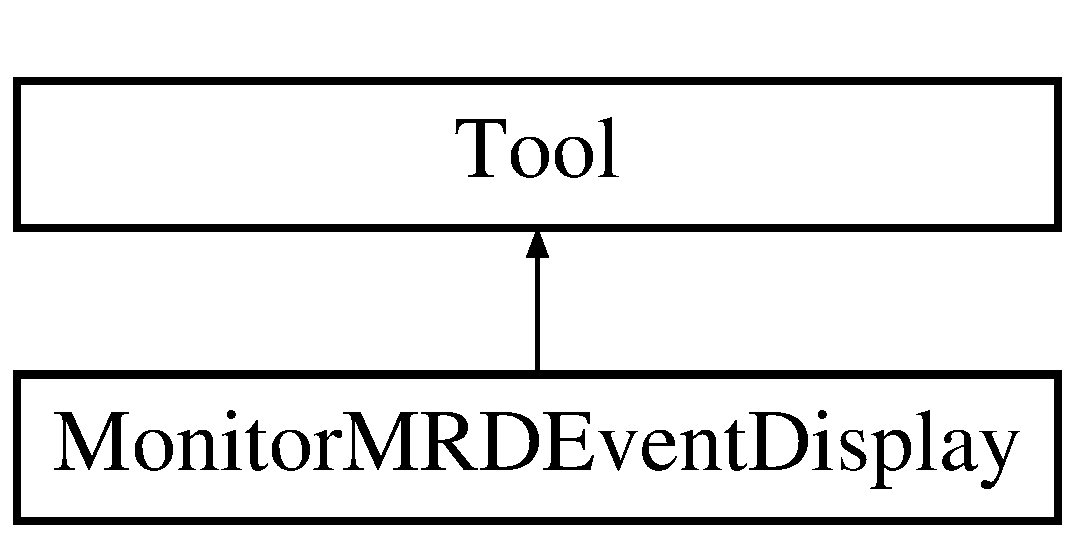
\includegraphics[height=2.000000cm]{classMonitorMRDEventDisplay}
\end{center}
\end{figure}
\subsection*{Public Member Functions}
\begin{DoxyCompactItemize}
\item 
\hypertarget{classMonitorMRDEventDisplay_a35e5b18f01d2249fe3d30a90c94a0692}{bool {\bfseries Initialise} (std\-::string configfile, \hyperlink{classDataModel}{Data\-Model} \&data)}\label{classMonitorMRDEventDisplay_a35e5b18f01d2249fe3d30a90c94a0692}

\item 
\hypertarget{classMonitorMRDEventDisplay_aa0046209bda6d93bd001b3326a6ec9ee}{bool {\bfseries Execute} ()}\label{classMonitorMRDEventDisplay_aa0046209bda6d93bd001b3326a6ec9ee}

\item 
\hypertarget{classMonitorMRDEventDisplay_a4241c27d6fbffa510cf2ab765367d96f}{bool {\bfseries Finalise} ()}\label{classMonitorMRDEventDisplay_a4241c27d6fbffa510cf2ab765367d96f}

\item 
\hypertarget{classMonitorMRDEventDisplay_af0cca0c4edd7afac1e6c5c6094e984e1}{void {\bfseries Initialize\-Vectors} ()}\label{classMonitorMRDEventDisplay_af0cca0c4edd7afac1e6c5c6094e984e1}

\item 
\hypertarget{classMonitorMRDEventDisplay_a39e8832209afa666872d8b3dfc043ea0}{void {\bfseries Erase\-Old\-Data} ()}\label{classMonitorMRDEventDisplay_a39e8832209afa666872d8b3dfc043ea0}

\item 
\hypertarget{classMonitorMRDEventDisplay_a939860a98875349b13946c622ca3fe41}{void {\bfseries Update\-Monitor\-Plots} ()}\label{classMonitorMRDEventDisplay_a939860a98875349b13946c622ca3fe41}

\end{DoxyCompactItemize}


The documentation for this class was generated from the following files\-:\begin{DoxyCompactItemize}
\item 
User\-Tools/\-Monitor\-M\-R\-D\-Event\-Display/Monitor\-M\-R\-D\-Event\-Display.\-h\item 
User\-Tools/\-Monitor\-M\-R\-D\-Event\-Display/Monitor\-M\-R\-D\-Event\-Display.\-cpp\end{DoxyCompactItemize}

\hypertarget{classMonitorMRDLive}{
\section{MonitorMRDLive Class Reference}
\label{classMonitorMRDLive}\index{MonitorMRDLive@{MonitorMRDLive}}
}
\subsection*{Public Member Functions}
\begin{DoxyCompactItemize}
\item 
\hypertarget{classMonitorMRDLive_a05a63a84f2a7b6e4340d21e2c018a971}{
bool {\bfseries Initialise} (std::string configfile, \hyperlink{classDataModel}{DataModel} \&data)}
\label{classMonitorMRDLive_a05a63a84f2a7b6e4340d21e2c018a971}

\item 
\hypertarget{classMonitorMRDLive_a86c7648cc8aad1fb24d86d7f13507128}{
bool {\bfseries Execute} ()}
\label{classMonitorMRDLive_a86c7648cc8aad1fb24d86d7f13507128}

\item 
\hypertarget{classMonitorMRDLive_ae061bd82e645e7cd1d383badee568d49}{
bool {\bfseries Finalise} ()}
\label{classMonitorMRDLive_ae061bd82e645e7cd1d383badee568d49}

\item 
\hypertarget{classMonitorMRDLive_a74930d4f7ddc5ff78db48551aa9d6f99}{
void {\bfseries MRDTDCPlots} ()}
\label{classMonitorMRDLive_a74930d4f7ddc5ff78db48551aa9d6f99}

\end{DoxyCompactItemize}


The documentation for this class was generated from the following files:\begin{DoxyCompactItemize}
\item 
UserTools/MonitorMRDLive/MonitorMRDLive.h\item 
UserTools/MonitorMRDLive/MonitorMRDLive.cpp\end{DoxyCompactItemize}

\hypertarget{classMonitorMRDTime}{\section{Monitor\-M\-R\-D\-Time Class Reference}
\label{classMonitorMRDTime}\index{Monitor\-M\-R\-D\-Time@{Monitor\-M\-R\-D\-Time}}
}
Inheritance diagram for Monitor\-M\-R\-D\-Time\-:\begin{figure}[H]
\begin{center}
\leavevmode
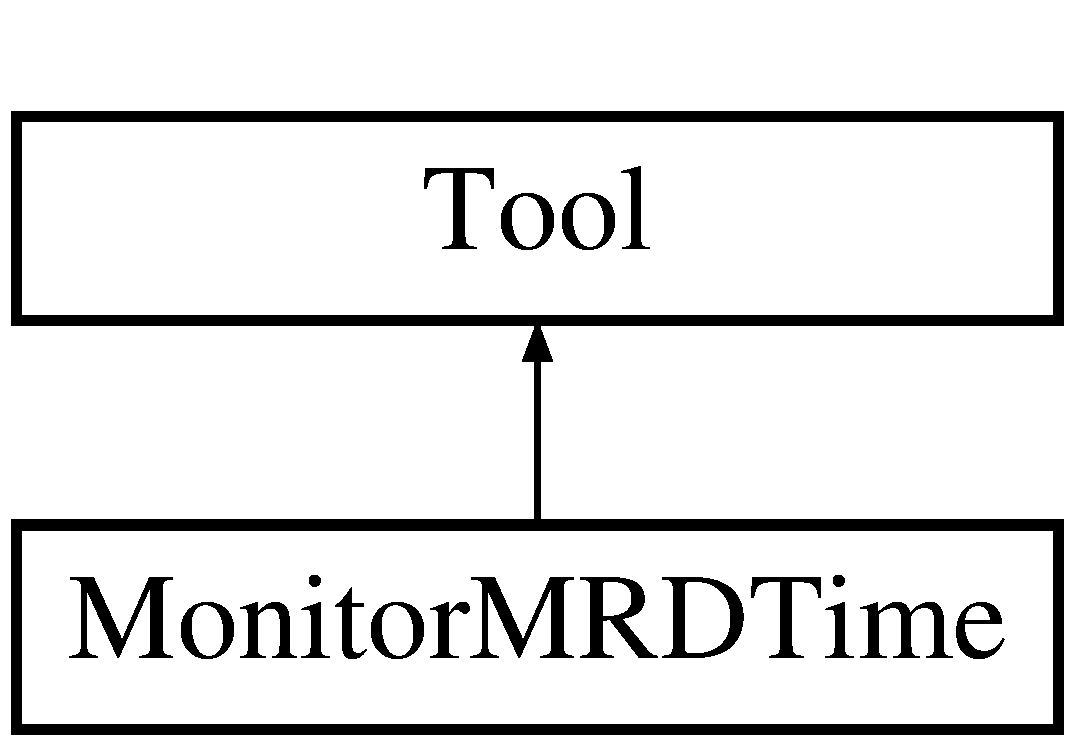
\includegraphics[height=2.000000cm]{classMonitorMRDTime}
\end{center}
\end{figure}
\subsection*{Public Member Functions}
\begin{DoxyCompactItemize}
\item 
\hypertarget{classMonitorMRDTime_a0eb95583c6a147059859b56c0c2687ee}{bool {\bfseries Initialise} (std\-::string configfile, \hyperlink{classDataModel}{Data\-Model} \&data)}\label{classMonitorMRDTime_a0eb95583c6a147059859b56c0c2687ee}

\item 
\hypertarget{classMonitorMRDTime_af322d7679b5199d91caec6ca69226995}{bool {\bfseries Execute} ()}\label{classMonitorMRDTime_af322d7679b5199d91caec6ca69226995}

\item 
\hypertarget{classMonitorMRDTime_ad9b436fb72af740b16468463a50eefe6}{bool {\bfseries Finalise} ()}\label{classMonitorMRDTime_ad9b436fb72af740b16468463a50eefe6}

\item 
\hypertarget{classMonitorMRDTime_affa1155c36568467e553b8e9460ecf8a}{void {\bfseries M\-R\-D\-Time\-Plots} ()}\label{classMonitorMRDTime_affa1155c36568467e553b8e9460ecf8a}

\item 
\hypertarget{classMonitorMRDTime_ad2e2bfb694d2bf99d189f7b4496da16a}{void {\bfseries Update\-Monitor\-Sources} ()}\label{classMonitorMRDTime_ad2e2bfb694d2bf99d189f7b4496da16a}

\item 
\hypertarget{classMonitorMRDTime_ad3380e8bac12fc88745a15dd0b68ed09}{void {\bfseries Fill\-Events} ()}\label{classMonitorMRDTime_ad3380e8bac12fc88745a15dd0b68ed09}

\item 
\hypertarget{classMonitorMRDTime_a3a81ee4967f10349d1f6571f7f4a8696}{void {\bfseries Initialize\-Vectors} ()}\label{classMonitorMRDTime_a3a81ee4967f10349d1f6571f7f4a8696}

\end{DoxyCompactItemize}


The documentation for this class was generated from the following files\-:\begin{DoxyCompactItemize}
\item 
User\-Tools/\-Monitor\-M\-R\-D\-Time/Monitor\-M\-R\-D\-Time.\-h\item 
User\-Tools/\-Monitor\-M\-R\-D\-Time/Monitor\-M\-R\-D\-Time.\-cpp\end{DoxyCompactItemize}

\hypertarget{classMonitorReceive}{\section{Monitor\-Receive Class Reference}
\label{classMonitorReceive}\index{Monitor\-Receive@{Monitor\-Receive}}
}
Inheritance diagram for Monitor\-Receive\-:\begin{figure}[H]
\begin{center}
\leavevmode
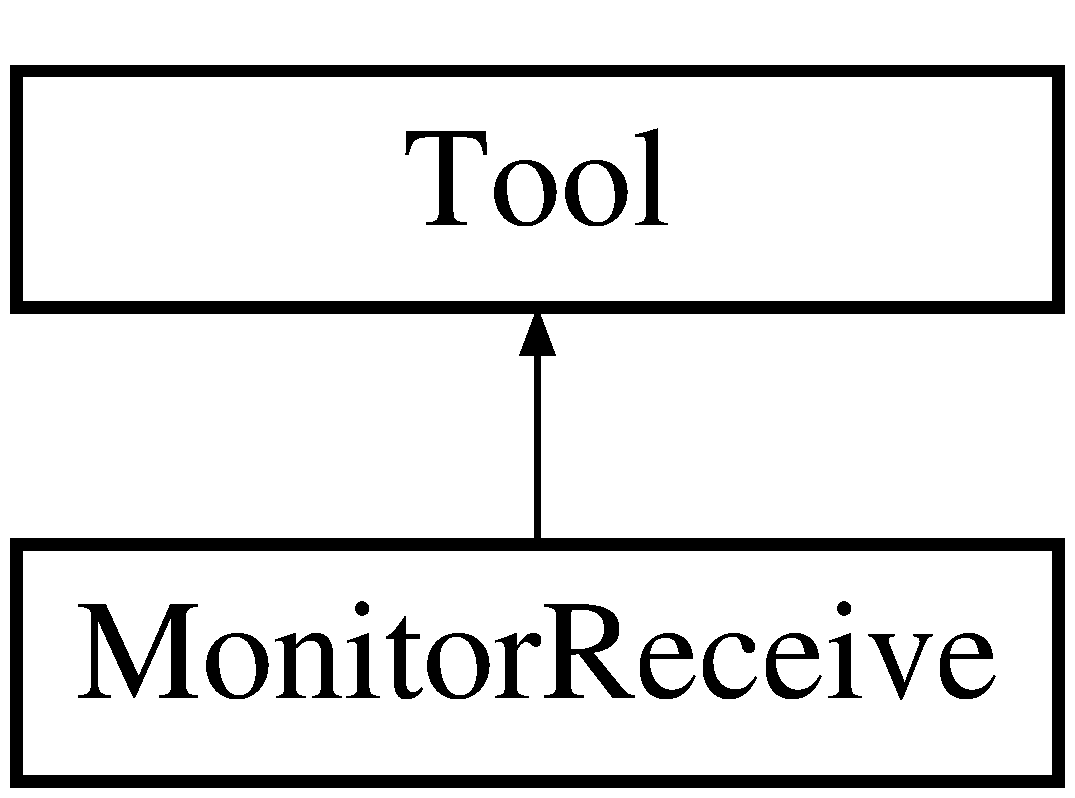
\includegraphics[height=2.000000cm]{classMonitorReceive}
\end{center}
\end{figure}
\subsection*{Public Member Functions}
\begin{DoxyCompactItemize}
\item 
\hypertarget{classMonitorReceive_a635e0cf91b53352483bb0f30a27c1287}{bool {\bfseries Initialise} (std\-::string configfile, \hyperlink{classDataModel}{Data\-Model} \&data)}\label{classMonitorReceive_a635e0cf91b53352483bb0f30a27c1287}

\item 
\hypertarget{classMonitorReceive_a316f1f7d2a21f698faa0cb8d0583c49a}{bool {\bfseries Execute} ()}\label{classMonitorReceive_a316f1f7d2a21f698faa0cb8d0583c49a}

\item 
\hypertarget{classMonitorReceive_a9f11f11200f7cca1cffc38d9021f831a}{bool {\bfseries Finalise} ()}\label{classMonitorReceive_a9f11f11200f7cca1cffc38d9021f831a}

\item 
\hypertarget{classMonitorReceive_a87daa52032531a34d499d4ca510a5627}{int {\bfseries Update\-Monitor\-Sources} ()}\label{classMonitorReceive_a87daa52032531a34d499d4ca510a5627}

\end{DoxyCompactItemize}


The documentation for this class was generated from the following files\-:\begin{DoxyCompactItemize}
\item 
User\-Tools/\-Monitor\-Receive/Monitor\-Receive.\-h\item 
User\-Tools/\-Monitor\-Receive/Monitor\-Receive.\-cpp\end{DoxyCompactItemize}

\hypertarget{classMonitorSimReceive}{
\section{MonitorSimReceive Class Reference}
\label{classMonitorSimReceive}\index{MonitorSimReceive@{MonitorSimReceive}}
}
\subsection*{Public Member Functions}
\begin{DoxyCompactItemize}
\item 
\hypertarget{classMonitorSimReceive_a3e841c945c5481d97fc82cb4658bdaee}{
bool {\bfseries Initialise} (std::string configfile, \hyperlink{classDataModel}{DataModel} \&data)}
\label{classMonitorSimReceive_a3e841c945c5481d97fc82cb4658bdaee}

\item 
\hypertarget{classMonitorSimReceive_a289c3a6508deff086d9250263cc9981e}{
bool {\bfseries Execute} ()}
\label{classMonitorSimReceive_a289c3a6508deff086d9250263cc9981e}

\item 
\hypertarget{classMonitorSimReceive_afb3fd0f4191c888966b83a0bc8ff032d}{
bool {\bfseries Finalise} ()}
\label{classMonitorSimReceive_afb3fd0f4191c888966b83a0bc8ff032d}

\end{DoxyCompactItemize}


The documentation for this class was generated from the following files:\begin{DoxyCompactItemize}
\item 
UserTools/MonitorSimReceive/MonitorSimReceive.h\item 
UserTools/MonitorSimReceive/MonitorSimReceive.cpp\end{DoxyCompactItemize}

\include{classMonitorTankLive}
\include{classMonitorTankTime}
\hypertarget{classMrdDiscriminatorScan}{
\section{MrdDiscriminatorScan Class Reference}
\label{classMrdDiscriminatorScan}\index{MrdDiscriminatorScan@{MrdDiscriminatorScan}}
}
\subsection*{Public Member Functions}
\begin{DoxyCompactItemize}
\item 
\hypertarget{classMrdDiscriminatorScan_abaa4b337b0df9e14620ae6f9b8794b1b}{
bool {\bfseries Initialise} (std::string configfile, \hyperlink{classDataModel}{DataModel} \&data)}
\label{classMrdDiscriminatorScan_abaa4b337b0df9e14620ae6f9b8794b1b}

\item 
\hypertarget{classMrdDiscriminatorScan_a37ebf1bcfc1bdaafe1afddea5bacbd67}{
bool {\bfseries Execute} ()}
\label{classMrdDiscriminatorScan_a37ebf1bcfc1bdaafe1afddea5bacbd67}

\item 
\hypertarget{classMrdDiscriminatorScan_a73fe6971470c0858f87051e2ab853e18}{
bool {\bfseries Finalise} ()}
\label{classMrdDiscriminatorScan_a73fe6971470c0858f87051e2ab853e18}

\end{DoxyCompactItemize}


The documentation for this class was generated from the following files:\begin{DoxyCompactItemize}
\item 
UserTools/MrdDiscriminatorScan/MrdDiscriminatorScan.h\item 
UserTools/MrdDiscriminatorScan/MrdDiscriminatorScan.cpp\end{DoxyCompactItemize}

\hypertarget{classMrdDistributions}{\section{Mrd\-Distributions Class Reference}
\label{classMrdDistributions}\index{Mrd\-Distributions@{Mrd\-Distributions}}
}
Inheritance diagram for Mrd\-Distributions\-:\begin{figure}[H]
\begin{center}
\leavevmode
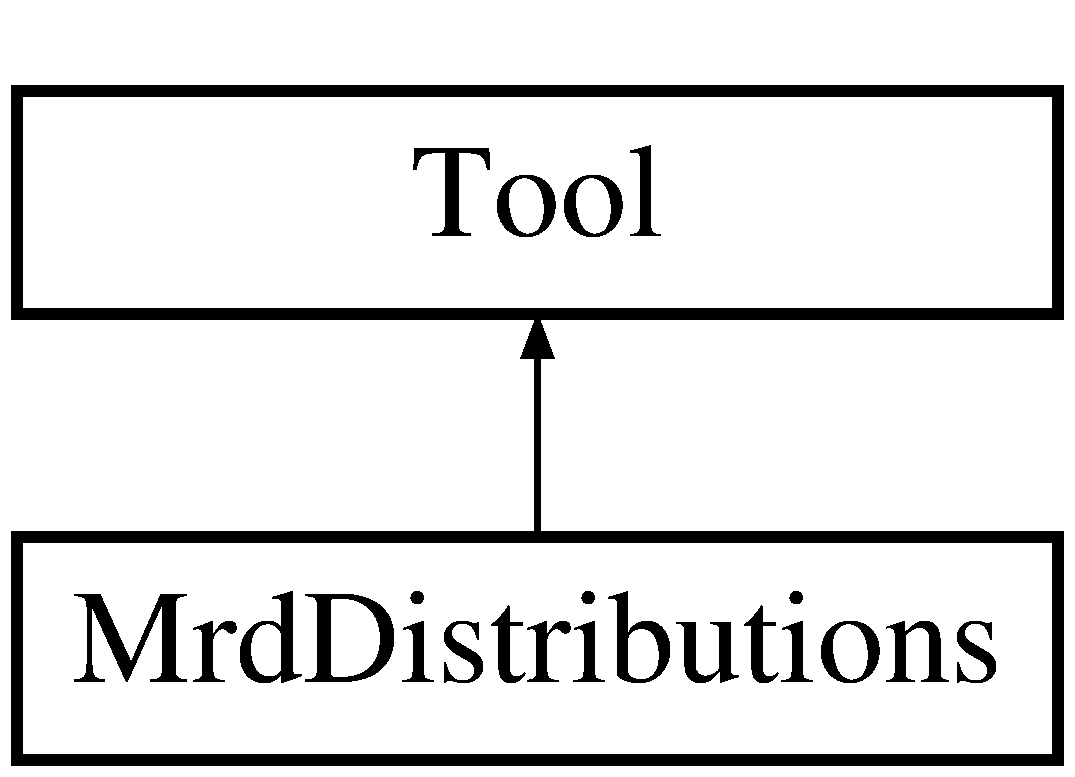
\includegraphics[height=2.000000cm]{classMrdDistributions}
\end{center}
\end{figure}
\subsection*{Public Member Functions}
\begin{DoxyCompactItemize}
\item 
\hypertarget{classMrdDistributions_a0e32e324d6f93d4a45b6b313fc1fb735}{bool {\bfseries Initialise} (std\-::string configfile, \hyperlink{classDataModel}{Data\-Model} \&data)}\label{classMrdDistributions_a0e32e324d6f93d4a45b6b313fc1fb735}

\item 
\hypertarget{classMrdDistributions_a9d925095cb7ff1ede865837076da0b03}{bool {\bfseries Execute} ()}\label{classMrdDistributions_a9d925095cb7ff1ede865837076da0b03}

\item 
\hypertarget{classMrdDistributions_acb7753d5c69220fabc7f93c9bd6f3948}{bool {\bfseries Finalise} ()}\label{classMrdDistributions_acb7753d5c69220fabc7f93c9bd6f3948}

\end{DoxyCompactItemize}
\subsection*{Public Attributes}
\begin{DoxyCompactItemize}
\item 
\hypertarget{classMrdDistributions_a47f2a560f640c946ed721acdf093ab95}{int {\bfseries verbosity} =1}\label{classMrdDistributions_a47f2a560f640c946ed721acdf093ab95}

\item 
\hypertarget{classMrdDistributions_acfa5709e73f4984f9bd4664d11e6ff39}{bool {\bfseries print\-Tracks}}\label{classMrdDistributions_acfa5709e73f4984f9bd4664d11e6ff39}

\item 
\hypertarget{classMrdDistributions_a5b40d02e337e41a40f52f78624bca5d5}{std\-::string {\bfseries plot\-Directory}}\label{classMrdDistributions_a5b40d02e337e41a40f52f78624bca5d5}

\end{DoxyCompactItemize}


The documentation for this class was generated from the following files\-:\begin{DoxyCompactItemize}
\item 
User\-Tools/\-Mrd\-Distributions/Mrd\-Distributions.\-h\item 
User\-Tools/\-Mrd\-Distributions/Mrd\-Distributions.\-cpp\end{DoxyCompactItemize}

\hypertarget{classMrdEfficiency}{
\section{MrdEfficiency Class Reference}
\label{classMrdEfficiency}\index{MrdEfficiency@{MrdEfficiency}}
}
\subsection*{Public Member Functions}
\begin{DoxyCompactItemize}
\item 
\hypertarget{classMrdEfficiency_a08728f36b55f16ae22b542b41af58c30}{
bool {\bfseries Initialise} (std::string configfile, \hyperlink{classDataModel}{DataModel} \&data)}
\label{classMrdEfficiency_a08728f36b55f16ae22b542b41af58c30}

\item 
\hypertarget{classMrdEfficiency_ada02439004731e9ab80cceaf5027ac77}{
bool {\bfseries Execute} ()}
\label{classMrdEfficiency_ada02439004731e9ab80cceaf5027ac77}

\item 
\hypertarget{classMrdEfficiency_a804e18645520f7ede27d4cd7d4a0d666}{
bool {\bfseries Finalise} ()}
\label{classMrdEfficiency_a804e18645520f7ede27d4cd7d4a0d666}

\end{DoxyCompactItemize}
\subsection*{Public Attributes}
\begin{DoxyCompactItemize}
\item 
\hypertarget{classMrdEfficiency_a96c39668e71df6a3e0261bf7aeac9dcb}{
int {\bfseries verbosity} = 1}
\label{classMrdEfficiency_a96c39668e71df6a3e0261bf7aeac9dcb}

\item 
\hypertarget{classMrdEfficiency_af3a7b151047b6f71fcf1333f869c6a72}{
bool {\bfseries drawHistos}}
\label{classMrdEfficiency_af3a7b151047b6f71fcf1333f869c6a72}

\end{DoxyCompactItemize}


The documentation for this class was generated from the following files:\begin{DoxyCompactItemize}
\item 
UserTools/MrdEfficiency/MrdEfficiency.h\item 
UserTools/MrdEfficiency/MrdEfficiency.cpp\end{DoxyCompactItemize}

\hypertarget{classMRDOut}{\section{M\-R\-D\-Out Class Reference}
\label{classMRDOut}\index{M\-R\-D\-Out@{M\-R\-D\-Out}}
}
Inheritance diagram for M\-R\-D\-Out\-:\begin{figure}[H]
\begin{center}
\leavevmode
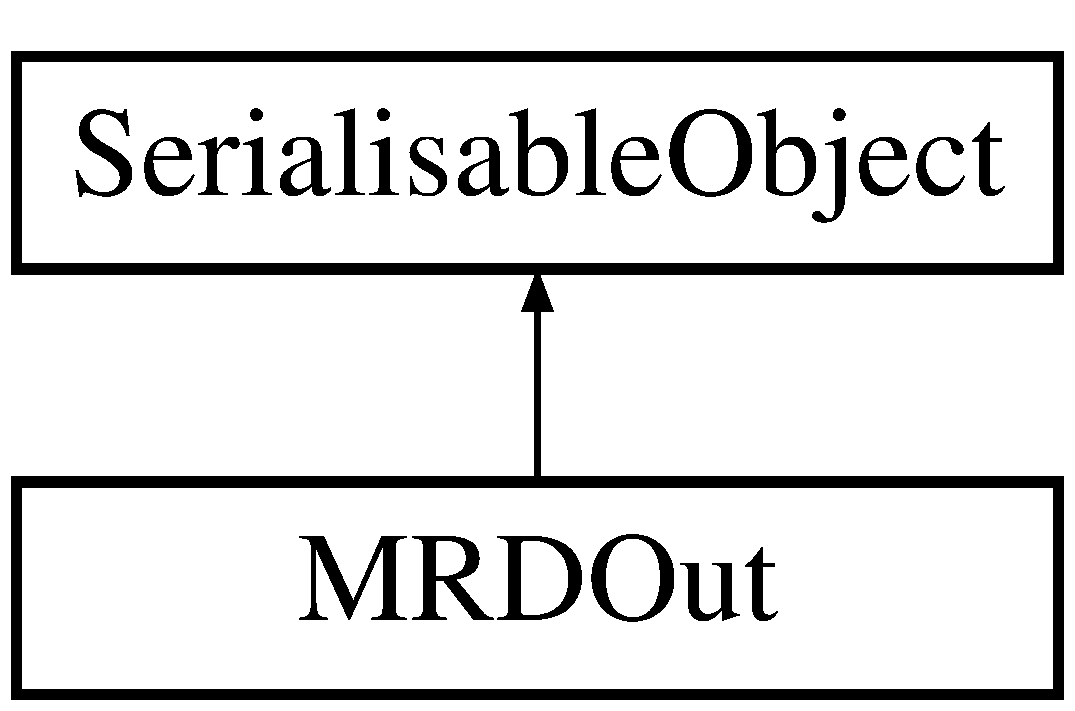
\includegraphics[height=2.000000cm]{classMRDOut}
\end{center}
\end{figure}
\subsection*{Public Member Functions}
\begin{DoxyCompactItemize}
\item 
\hypertarget{classMRDOut_a2c72c51c7288bd4ed73d4c9de0509150}{bool {\bfseries Send} (zmq\-::socket\-\_\-t $\ast$socket)}\label{classMRDOut_a2c72c51c7288bd4ed73d4c9de0509150}

\item 
\hypertarget{classMRDOut_a7e83eb6f2ac421109f907235d4211571}{bool {\bfseries Receive} (zmq\-::socket\-\_\-t $\ast$socket)}\label{classMRDOut_a7e83eb6f2ac421109f907235d4211571}

\item 
\hypertarget{classMRDOut_a956aa4f1b5746c9e12e7b69980d58b62}{bool {\bfseries Print} ()}\label{classMRDOut_a956aa4f1b5746c9e12e7b69980d58b62}

\end{DoxyCompactItemize}
\subsection*{Public Attributes}
\begin{DoxyCompactItemize}
\item 
\hypertarget{classMRDOut_a99fcd630b69a452e867b30bda86b9d6c}{unsigned int {\bfseries Out\-N}}\label{classMRDOut_a99fcd630b69a452e867b30bda86b9d6c}

\item 
\hypertarget{classMRDOut_aefae0cae9b9149247c66fec5140393af}{unsigned int {\bfseries Trigger}}\label{classMRDOut_aefae0cae9b9149247c66fec5140393af}

\item 
\hypertarget{classMRDOut_ae8b80ae7773fb9573a26cf791e18995d}{std\-::vector$<$ unsigned int $>$ {\bfseries Value}}\label{classMRDOut_ae8b80ae7773fb9573a26cf791e18995d}

\item 
\hypertarget{classMRDOut_a03e751accc75934f1ad7926415ce570e}{std\-::vector$<$ unsigned int $>$ {\bfseries Slot}}\label{classMRDOut_a03e751accc75934f1ad7926415ce570e}

\item 
\hypertarget{classMRDOut_a7849667340cd72441d429608ff9b98f9}{std\-::vector$<$ unsigned int $>$ {\bfseries Channel}}\label{classMRDOut_a7849667340cd72441d429608ff9b98f9}

\item 
\hypertarget{classMRDOut_a518db4f65639b83f1e1bcf42f31c1076}{std\-::vector$<$ unsigned int $>$ {\bfseries Crate}}\label{classMRDOut_a518db4f65639b83f1e1bcf42f31c1076}

\item 
\hypertarget{classMRDOut_aa943ba9150d67e2e1758b24324b4ae21}{std\-::vector$<$ std\-::string $>$ {\bfseries Type}}\label{classMRDOut_aa943ba9150d67e2e1758b24324b4ae21}

\item 
\hypertarget{classMRDOut_a1541d7fe5112f7932ec54b285c13eb08}{long {\bfseries Time\-Stamp}}\label{classMRDOut_a1541d7fe5112f7932ec54b285c13eb08}

\end{DoxyCompactItemize}
\subsection*{Friends}
\begin{DoxyCompactItemize}
\item 
\hypertarget{classMRDOut_ac98d07dd8f7b70e16ccb9a01abf56b9c}{class {\bfseries boost\-::serialization\-::access}}\label{classMRDOut_ac98d07dd8f7b70e16ccb9a01abf56b9c}

\end{DoxyCompactItemize}


The documentation for this class was generated from the following files\-:\begin{DoxyCompactItemize}
\item 
Data\-Model/M\-R\-D\-Out.\-h\item 
Data\-Model/M\-R\-D\-Out.\-cpp\end{DoxyCompactItemize}

\hypertarget{classMrdPaddlePlot}{
\section{MrdPaddlePlot Class Reference}
\label{classMrdPaddlePlot}\index{MrdPaddlePlot@{MrdPaddlePlot}}
}
\subsection*{Public Member Functions}
\begin{DoxyCompactItemize}
\item 
\hypertarget{classMrdPaddlePlot_a17a420342671b900521987f9dc070985}{
bool {\bfseries Initialise} (std::string configfile, \hyperlink{classDataModel}{DataModel} \&data)}
\label{classMrdPaddlePlot_a17a420342671b900521987f9dc070985}

\item 
\hypertarget{classMrdPaddlePlot_a655db67bffdbd48ef56a928bb84be1c2}{
bool {\bfseries Execute} ()}
\label{classMrdPaddlePlot_a655db67bffdbd48ef56a928bb84be1c2}

\item 
\hypertarget{classMrdPaddlePlot_ada0f5bfebebcd67b1da1f9db55fb13bc}{
bool {\bfseries Finalise} ()}
\label{classMrdPaddlePlot_ada0f5bfebebcd67b1da1f9db55fb13bc}

\end{DoxyCompactItemize}


The documentation for this class was generated from the following files:\begin{DoxyCompactItemize}
\item 
UserTools/MrdPaddlePlot/MrdPaddlePlot.h\item 
UserTools/MrdPaddlePlot/MrdPaddlePlot.cpp\end{DoxyCompactItemize}

\hypertarget{classMRDPulseFinder}{\section{M\-R\-D\-Pulse\-Finder Class Reference}
\label{classMRDPulseFinder}\index{M\-R\-D\-Pulse\-Finder@{M\-R\-D\-Pulse\-Finder}}
}
Inheritance diagram for M\-R\-D\-Pulse\-Finder\-:\begin{figure}[H]
\begin{center}
\leavevmode
\includegraphics[height=2.000000cm]{classMRDPulseFinder}
\end{center}
\end{figure}
\subsection*{Public Member Functions}
\begin{DoxyCompactItemize}
\item 
\hypertarget{classMRDPulseFinder_ad64f6c541f6d5cc2cb1036a9249837c5}{bool {\bfseries Initialise} (std\-::string configfile, \hyperlink{classDataModel}{Data\-Model} \&data)}\label{classMRDPulseFinder_ad64f6c541f6d5cc2cb1036a9249837c5}

\item 
\hypertarget{classMRDPulseFinder_adff581ca17c601b5ec24a96ad6b85941}{bool {\bfseries Execute} ()}\label{classMRDPulseFinder_adff581ca17c601b5ec24a96ad6b85941}

\item 
\hypertarget{classMRDPulseFinder_a492f228151d4af0a6f07e21ff7e732b0}{bool {\bfseries Finalise} ()}\label{classMRDPulseFinder_a492f228151d4af0a6f07e21ff7e732b0}

\item 
\hypertarget{classMRDPulseFinder_ab82aeb6cbc87a8d0f88252335f261d33}{std\-::vector$<$ \hyperlink{classADCPulse}{A\-D\-C\-Pulse} $>$ {\bfseries Find\-Pulse} (vector$<$ short unsigned int $>$ $\ast$some\-Wave)}\label{classMRDPulseFinder_ab82aeb6cbc87a8d0f88252335f261d33}

\end{DoxyCompactItemize}


The documentation for this class was generated from the following files\-:\begin{DoxyCompactItemize}
\item 
User\-Tools/\-M\-R\-D\-Pulse\-Finder/M\-R\-D\-Pulse\-Finder.\-h\item 
User\-Tools/\-M\-R\-D\-Pulse\-Finder/M\-R\-D\-Pulse\-Finder.\-cpp\end{DoxyCompactItemize}

\include{classMrdStub}
\hypertarget{classMRDTree}{
\section{MRDTree Class Reference}
\label{classMRDTree}\index{MRDTree@{MRDTree}}
}
\subsection*{Public Member Functions}
\begin{DoxyCompactItemize}
\item 
\hypertarget{classMRDTree_aeab336bcc0233f344b19f18cf879d65c}{
{\bfseries MRDTree} (TTree $\ast$tree=0)}
\label{classMRDTree_aeab336bcc0233f344b19f18cf879d65c}

\item 
\hypertarget{classMRDTree_ae43262ad3a6551b4617a3c046825f9f1}{
virtual Int\_\-t {\bfseries Cut} (Long64\_\-t entry)}
\label{classMRDTree_ae43262ad3a6551b4617a3c046825f9f1}

\item 
\hypertarget{classMRDTree_a1b46188d4d4b9f5c9d7e63c7305ab5ef}{
virtual Int\_\-t {\bfseries GetEntry} (Long64\_\-t entry)}
\label{classMRDTree_a1b46188d4d4b9f5c9d7e63c7305ab5ef}

\item 
\hypertarget{classMRDTree_ac4b67ff34ead1d39c5d324462e988726}{
virtual Long64\_\-t {\bfseries LoadTree} (Long64\_\-t entry)}
\label{classMRDTree_ac4b67ff34ead1d39c5d324462e988726}

\item 
\hypertarget{classMRDTree_ac380b6dac4ef6d6aecc09f3f90c4f3f6}{
virtual void {\bfseries Init} (TTree $\ast$tree)}
\label{classMRDTree_ac380b6dac4ef6d6aecc09f3f90c4f3f6}

\item 
\hypertarget{classMRDTree_abf8580954488c13d66eed0dde60f96b4}{
virtual void {\bfseries Loop} ()}
\label{classMRDTree_abf8580954488c13d66eed0dde60f96b4}

\item 
\hypertarget{classMRDTree_acb7f53057ebdd2a594b07c1294b5dde4}{
virtual Bool\_\-t {\bfseries Notify} ()}
\label{classMRDTree_acb7f53057ebdd2a594b07c1294b5dde4}

\item 
\hypertarget{classMRDTree_aec15bed544906066fdc89e749ef181aa}{
virtual void {\bfseries Show} (Long64\_\-t entry=-\/1)}
\label{classMRDTree_aec15bed544906066fdc89e749ef181aa}

\end{DoxyCompactItemize}
\subsection*{Public Attributes}
\begin{DoxyCompactItemize}
\item 
\hypertarget{classMRDTree_a73df1663124477ad3347f5a894801079}{
TTree $\ast$ {\bfseries fChain}}
\label{classMRDTree_a73df1663124477ad3347f5a894801079}

\item 
\hypertarget{classMRDTree_ae34a2e8a27b9deafeb5d28677c4fe090}{
Int\_\-t \hyperlink{classMRDTree_ae34a2e8a27b9deafeb5d28677c4fe090}{fCurrent}}
\label{classMRDTree_ae34a2e8a27b9deafeb5d28677c4fe090}

\begin{DoxyCompactList}\small\item\em pointer to the analyzed TTree or TChain \item\end{DoxyCompactList}\item 
\hypertarget{classMRDTree_acbb905703b5bd9054df1c685fce4c340}{
UInt\_\-t \hyperlink{classMRDTree_acbb905703b5bd9054df1c685fce4c340}{Trigger}}
\label{classMRDTree_acbb905703b5bd9054df1c685fce4c340}

\begin{DoxyCompactList}\small\item\em current Tree number in a TChain \item\end{DoxyCompactList}\item 
\hypertarget{classMRDTree_ad3a57b2d0d73f13d4fc46d8c3e0c0db8}{
UInt\_\-t {\bfseries OutNumber}}
\label{classMRDTree_ad3a57b2d0d73f13d4fc46d8c3e0c0db8}

\item 
\hypertarget{classMRDTree_aad0e5fe201d44d17706919f231f23b6f}{
std::vector$<$ std::string $>$ $\ast$ {\bfseries Type}}
\label{classMRDTree_aad0e5fe201d44d17706919f231f23b6f}

\item 
\hypertarget{classMRDTree_ad30e310155b90d3d76025fba93cb1082}{
std::vector$<$ unsigned int $>$ $\ast$ {\bfseries Value}}
\label{classMRDTree_ad30e310155b90d3d76025fba93cb1082}

\item 
\hypertarget{classMRDTree_ad8a1fdd22f8e261bcc10527ae89aabc3}{
std::vector$<$ unsigned int $>$ $\ast$ {\bfseries Slot}}
\label{classMRDTree_ad8a1fdd22f8e261bcc10527ae89aabc3}

\item 
\hypertarget{classMRDTree_a4275330c81a0e7d017c473e88275dbc7}{
std::vector$<$ unsigned int $>$ $\ast$ {\bfseries Channel}}
\label{classMRDTree_a4275330c81a0e7d017c473e88275dbc7}

\item 
\hypertarget{classMRDTree_abee67bfdf0a6eaf117b85b9b2485612b}{
ULong64\_\-t {\bfseries TimeStamp}}
\label{classMRDTree_abee67bfdf0a6eaf117b85b9b2485612b}

\item 
\hypertarget{classMRDTree_a555f128842c285877adad7754222feb4}{
TBranch $\ast$ {\bfseries b\_\-Trigger}}
\label{classMRDTree_a555f128842c285877adad7754222feb4}

\item 
\hypertarget{classMRDTree_abee621e9208bdfcbdb2c2f068e74950d}{
TBranch $\ast$ {\bfseries b\_\-OutN}}
\label{classMRDTree_abee621e9208bdfcbdb2c2f068e74950d}

\item 
\hypertarget{classMRDTree_ae95ac23e8ade856062ca8646cf8b652e}{
TBranch $\ast$ {\bfseries b\_\-Type}}
\label{classMRDTree_ae95ac23e8ade856062ca8646cf8b652e}

\item 
\hypertarget{classMRDTree_ab5ec56917aad8639be559941dbbbf5f1}{
TBranch $\ast$ {\bfseries b\_\-Value}}
\label{classMRDTree_ab5ec56917aad8639be559941dbbbf5f1}

\item 
\hypertarget{classMRDTree_a7e22be6df66f4f8da01a836c6ba21251}{
TBranch $\ast$ {\bfseries b\_\-Slot}}
\label{classMRDTree_a7e22be6df66f4f8da01a836c6ba21251}

\item 
\hypertarget{classMRDTree_a3bb90cc6b5552840b91dfb88ce24d19e}{
TBranch $\ast$ {\bfseries b\_\-Channel}}
\label{classMRDTree_a3bb90cc6b5552840b91dfb88ce24d19e}

\item 
\hypertarget{classMRDTree_acc8785e5ee2f2702f240bfc1f629decc}{
TBranch $\ast$ {\bfseries b\_\-TimeStamp}}
\label{classMRDTree_acc8785e5ee2f2702f240bfc1f629decc}

\end{DoxyCompactItemize}


The documentation for this class was generated from the following files:\begin{DoxyCompactItemize}
\item 
UserTools/LoadCCData/MRDTree.h\item 
UserTools/LoadCCData/MRDTree.cpp\end{DoxyCompactItemize}

\hypertarget{classMyTool}{
\section{MyTool Class Reference}
\label{classMyTool}\index{MyTool@{MyTool}}
}


{\ttfamily \#include $<$MyTool.h$>$}\subsection*{Public Member Functions}
\begin{DoxyCompactItemize}
\item 
\hypertarget{classMyTool_ad85b796bdd675ae22e69cf40fe7b6314}{
\hyperlink{classMyTool_ad85b796bdd675ae22e69cf40fe7b6314}{MyTool} ()}
\label{classMyTool_ad85b796bdd675ae22e69cf40fe7b6314}

\begin{DoxyCompactList}\small\item\em Simple constructor. \item\end{DoxyCompactList}\item 
bool \hyperlink{classMyTool_a3bf60061195a18542c4cfb2916b9dad9}{Initialise} (std::string configfile, \hyperlink{classDataModel}{DataModel} \&data)
\begin{DoxyCompactList}\small\item\em Initialise Function for setting up Tool resources. \item\end{DoxyCompactList}\item 
\hypertarget{classMyTool_a0a58122023af90b9200d0e71e89cfb36}{
bool \hyperlink{classMyTool_a0a58122023af90b9200d0e71e89cfb36}{Execute} ()}
\label{classMyTool_a0a58122023af90b9200d0e71e89cfb36}

\begin{DoxyCompactList}\small\item\em Execute function used to perform Tool purpose. \item\end{DoxyCompactList}\item 
\hypertarget{classMyTool_a060ec6356451aa335d0de41093c9992f}{
bool \hyperlink{classMyTool_a060ec6356451aa335d0de41093c9992f}{Finalise} ()}
\label{classMyTool_a060ec6356451aa335d0de41093c9992f}

\begin{DoxyCompactList}\small\item\em Finalise function used to clean up resources. \item\end{DoxyCompactList}\end{DoxyCompactItemize}


\subsection{Detailed Description}
This is a blank template for a Tool used by the script to generate a new custom tool. Please fill out the description and author information.

Author}
B.Richards Date}
2019/05/28 10:44:00 Contact: \href{mailto:b.richards@qmul.ac.uk}{\tt b.richards@qmul.ac.uk} 

\subsection{Member Function Documentation}
\hypertarget{classMyTool_a3bf60061195a18542c4cfb2916b9dad9}{
\index{MyTool@{MyTool}!Initialise@{Initialise}}
\index{Initialise@{Initialise}!MyTool@{MyTool}}
\subsubsection[{Initialise}]{\setlength{\rightskip}{0pt plus 5cm}bool MyTool::Initialise (std::string {\em configfile}, \/  {\bf DataModel} \& {\em data})}}
\label{classMyTool_a3bf60061195a18542c4cfb2916b9dad9}


Initialise Function for setting up Tool resources. 
\begin{DoxyParams}{Parameters}
\item[{\em configfile}]The path and name of the dynamic configuration file to read in. \item[{\em data}]A reference to the transient data class used to pass information between Tools. \end{DoxyParams}


The documentation for this class was generated from the following files:\begin{DoxyCompactItemize}
\item 
UserTools/template/MyTool.h\item 
UserTools/template/MyTool.cpp\end{DoxyCompactItemize}

\hypertarget{structNCVPositionInfo}{\section{N\-C\-V\-Position\-Info Struct Reference}
\label{structNCVPositionInfo}\index{N\-C\-V\-Position\-Info@{N\-C\-V\-Position\-Info}}
}
\subsection*{Public Attributes}
\begin{DoxyCompactItemize}
\item 
\hypertarget{structNCVPositionInfo_ace4afc2346cc29522e1732f9f41de8dd}{double {\bfseries total\-\_\-\-P\-O\-T} = 0.}\label{structNCVPositionInfo_ace4afc2346cc29522e1732f9f41de8dd}

\item 
\hypertarget{structNCVPositionInfo_a813f7edef83ad94a009257ece03392dd}{uint64\-\_\-t {\bfseries num\-\_\-beam\-\_\-spills} = 0ull}\label{structNCVPositionInfo_a813f7edef83ad94a009257ece03392dd}

\item 
\hypertarget{structNCVPositionInfo_aa9303f33637e7e3f3a47dbc1ec915e97}{uint64\-\_\-t {\bfseries num\-\_\-source\-\_\-triggers} = 0ull}\label{structNCVPositionInfo_aa9303f33637e7e3f3a47dbc1ec915e97}

\item 
\hypertarget{structNCVPositionInfo_a5e5afcbdc00981d16728e325c0a8eca9}{uint64\-\_\-t {\bfseries num\-\_\-cosmic\-\_\-triggers} = 0ull}\label{structNCVPositionInfo_a5e5afcbdc00981d16728e325c0a8eca9}

\item 
\hypertarget{structNCVPositionInfo_ac4c3befd94418e04f02d2549569bd5eb}{uint64\-\_\-t {\bfseries num\-\_\-soft\-\_\-triggers} = 0ull}\label{structNCVPositionInfo_ac4c3befd94418e04f02d2549569bd5eb}

\end{DoxyCompactItemize}


The documentation for this struct was generated from the following file\-:\begin{DoxyCompactItemize}
\item 
User\-Tools/\-Phase\-I\-Tree\-Maker/Phase\-I\-Tree\-Maker.\-h\end{DoxyCompactItemize}

\hypertarget{classNeutronStudyPMCS}{\section{Neutron\-Study\-P\-M\-C\-S Class Reference}
\label{classNeutronStudyPMCS}\index{Neutron\-Study\-P\-M\-C\-S@{Neutron\-Study\-P\-M\-C\-S}}
}
Inheritance diagram for Neutron\-Study\-P\-M\-C\-S\-:\begin{figure}[H]
\begin{center}
\leavevmode
\includegraphics[height=2.000000cm]{classNeutronStudyPMCS}
\end{center}
\end{figure}
\subsection*{Public Member Functions}
\begin{DoxyCompactItemize}
\item 
\hypertarget{classNeutronStudyPMCS_a044b07d39e07fbac5764b8788f11a3ec}{bool {\bfseries Initialise} (std\-::string configfile, \hyperlink{classDataModel}{Data\-Model} \&data)}\label{classNeutronStudyPMCS_a044b07d39e07fbac5764b8788f11a3ec}

\item 
\hypertarget{classNeutronStudyPMCS_a1cc06822548c3febc0708db5b59c343b}{bool {\bfseries Execute} ()}\label{classNeutronStudyPMCS_a1cc06822548c3febc0708db5b59c343b}

\item 
\hypertarget{classNeutronStudyPMCS_aa4e1c744c42f16c63b4ddefefda81922}{bool {\bfseries Finalise} ()}\label{classNeutronStudyPMCS_aa4e1c744c42f16c63b4ddefefda81922}

\item 
\hypertarget{classNeutronStudyPMCS_acdaa5568f44221b53168e490969393bf}{double {\bfseries nu\-E\-Efficiency} (double nu\-E)}\label{classNeutronStudyPMCS_acdaa5568f44221b53168e490969393bf}

\item 
\hypertarget{classNeutronStudyPMCS_aefc2ab996c1c513c0f032931f3f67e7e}{double {\bfseries Muon\-Efficiency} (double mu\-\_\-\-E, double mu\-\_\-angle)}\label{classNeutronStudyPMCS_aefc2ab996c1c513c0f032931f3f67e7e}

\item 
\hypertarget{classNeutronStudyPMCS_ad0cfe53c957f4a47fbe60f7bc390e32b}{double {\bfseries Pion\-Inefficiency} (double pi\-\_\-\-E, double pi\-\_\-angle)}\label{classNeutronStudyPMCS_ad0cfe53c957f4a47fbe60f7bc390e32b}

\item 
\hypertarget{classNeutronStudyPMCS_aa55a9508e67f6c758b1e7ecb7ff87a74}{double {\bfseries Mu\-Esmear} (double mu\-\_\-\-E, double Eres)}\label{classNeutronStudyPMCS_aa55a9508e67f6c758b1e7ecb7ff87a74}

\item 
\hypertarget{classNeutronStudyPMCS_ad04d525456090178ee877757d120993a}{double {\bfseries Mu\-Anglesmear} (double mu\-\_\-px, double mu\-\_\-py, double mu\-\_\-pz, double angsmear)}\label{classNeutronStudyPMCS_ad04d525456090178ee877757d120993a}

\item 
\hypertarget{classNeutronStudyPMCS_a87bfadcdde1434cd4aaa66ff9968a121}{double {\bfseries Reco\-E} (double mu\-\_\-\-E, double mu\-\_\-angle)}\label{classNeutronStudyPMCS_a87bfadcdde1434cd4aaa66ff9968a121}

\item 
\hypertarget{classNeutronStudyPMCS_aadac422e432f47ceae16a87a8d2679bb}{int {\bfseries Detected\-Neutrons} (int totneut)}\label{classNeutronStudyPMCS_aadac422e432f47ceae16a87a8d2679bb}

\item 
\hypertarget{classNeutronStudyPMCS_a73c188dfa2d0465729cc3e7c2d68a1bd}{int {\bfseries Bkg\-Neutrons} (double prob)}\label{classNeutronStudyPMCS_a73c188dfa2d0465729cc3e7c2d68a1bd}

\end{DoxyCompactItemize}


The documentation for this class was generated from the following files\-:\begin{DoxyCompactItemize}
\item 
User\-Tools/\-Neutron\-Study\-P\-M\-C\-S/Neutron\-Study\-P\-M\-C\-S.\-h\item 
User\-Tools/\-Neutron\-Study\-P\-M\-C\-S/Neutron\-Study\-P\-M\-C\-S.\-cpp\end{DoxyCompactItemize}

\hypertarget{classNeutronStudyReadSandbox}{\section{Neutron\-Study\-Read\-Sandbox Class Reference}
\label{classNeutronStudyReadSandbox}\index{Neutron\-Study\-Read\-Sandbox@{Neutron\-Study\-Read\-Sandbox}}
}
Inheritance diagram for Neutron\-Study\-Read\-Sandbox\-:\begin{figure}[H]
\begin{center}
\leavevmode
\includegraphics[height=2.000000cm]{classNeutronStudyReadSandbox}
\end{center}
\end{figure}
\subsection*{Public Member Functions}
\begin{DoxyCompactItemize}
\item 
\hypertarget{classNeutronStudyReadSandbox_a9e73e205358244c86e066bb28266066f}{bool {\bfseries Initialise} (std\-::string configfile, \hyperlink{classDataModel}{Data\-Model} \&data)}\label{classNeutronStudyReadSandbox_a9e73e205358244c86e066bb28266066f}

\item 
\hypertarget{classNeutronStudyReadSandbox_a580157d5a29b14c99e698f0919b65049}{bool {\bfseries Execute} ()}\label{classNeutronStudyReadSandbox_a580157d5a29b14c99e698f0919b65049}

\item 
\hypertarget{classNeutronStudyReadSandbox_af76eafb91eaf9270a9423e15026d8e20}{bool {\bfseries Finalise} ()}\label{classNeutronStudyReadSandbox_af76eafb91eaf9270a9423e15026d8e20}

\end{DoxyCompactItemize}


The documentation for this class was generated from the following files\-:\begin{DoxyCompactItemize}
\item 
User\-Tools/\-Neutron\-Study\-Read\-Sandbox/Neutron\-Study\-Read\-Sandbox.\-h\item 
User\-Tools/\-Neutron\-Study\-Read\-Sandbox/Neutron\-Study\-Read\-Sandbox.\-cpp\end{DoxyCompactItemize}

\hypertarget{classNeutronStudyWriteTree}{
\section{NeutronStudyWriteTree Class Reference}
\label{classNeutronStudyWriteTree}\index{NeutronStudyWriteTree@{NeutronStudyWriteTree}}
}
\subsection*{Public Member Functions}
\begin{DoxyCompactItemize}
\item 
\hypertarget{classNeutronStudyWriteTree_a6fa5e7ec01a703b7589583e8c5af744d}{
bool {\bfseries Initialise} (std::string configfile, \hyperlink{classDataModel}{DataModel} \&data)}
\label{classNeutronStudyWriteTree_a6fa5e7ec01a703b7589583e8c5af744d}

\item 
\hypertarget{classNeutronStudyWriteTree_a9e89fb86ad252f39f5f173e0bd8f3528}{
bool {\bfseries Execute} ()}
\label{classNeutronStudyWriteTree_a9e89fb86ad252f39f5f173e0bd8f3528}

\item 
\hypertarget{classNeutronStudyWriteTree_ad11e2482834166c4630ddf4cd8fd6d38}{
bool {\bfseries Finalise} ()}
\label{classNeutronStudyWriteTree_ad11e2482834166c4630ddf4cd8fd6d38}

\end{DoxyCompactItemize}


The documentation for this class was generated from the following files:\begin{DoxyCompactItemize}
\item 
UserTools/NeutronStudyWriteTree/NeutronStudyWriteTree.h\item 
UserTools/NeutronStudyWriteTree/NeutronStudyWriteTree.cpp\end{DoxyCompactItemize}

\include{classnnls}
\include{classnnlsmatrix}
\include{classNnlsSolution}
\include{classnnlsvector}
\include{classPaddle}
\hypertarget{classParameters}{\section{Parameters Class Reference}
\label{classParameters}\index{Parameters@{Parameters}}
}
\subsection*{Public Member Functions}
\begin{DoxyCompactItemize}
\item 
\hypertarget{classParameters_ad51d449c4d2963bef72fde2308966d8b}{void {\bfseries Run\-Print\-Parameters} ()}\label{classParameters_ad51d449c4d2963bef72fde2308966d8b}

\item 
\hypertarget{classParameters_a08f0965d2fe93066d0c550f08716829d}{void {\bfseries Set\-Simple\-Time\-Resolution} ()}\label{classParameters_a08f0965d2fe93066d0c550f08716829d}

\item 
\hypertarget{classParameters_ac1d25752b880deb537aa4344b40dca5e}{bool {\bfseries Simple\-Time\-Resolution} ()}\label{classParameters_ac1d25752b880deb537aa4344b40dca5e}

\item 
\hypertarget{classParameters_ac11f733ad0fa1552e523972433cbe0d1}{void {\bfseries Set\-Simple\-Time\-Slew} ()}\label{classParameters_ac11f733ad0fa1552e523972433cbe0d1}

\item 
\hypertarget{classParameters_aff94a6d602c527a3690cd1e79970b00b}{bool {\bfseries Simple\-Time\-Slew} ()}\label{classParameters_aff94a6d602c527a3690cd1e79970b00b}

\item 
\hypertarget{classParameters_a7c15c7be2a780eb1110ee3767eea4555}{void {\bfseries Set\-Simple\-Refractive\-Index} ()}\label{classParameters_a7c15c7be2a780eb1110ee3767eea4555}

\item 
\hypertarget{classParameters_a66a9a682eff6bf1f55aae967da3f7beb}{bool {\bfseries Simple\-Refractive\-Index} ()}\label{classParameters_a66a9a682eff6bf1f55aae967da3f7beb}

\item 
\hypertarget{classParameters_a593ddf265554ac4fb05f86d9ac82bc7a}{double {\bfseries Get\-Cherenkov\-Angle} ()}\label{classParameters_a593ddf265554ac4fb05f86d9ac82bc7a}

\item 
\hypertarget{classParameters_a754e96439c2c90e10337737055fbae8a}{double {\bfseries Get\-Time\-Resolution} (double Q)}\label{classParameters_a754e96439c2c90e10337737055fbae8a}

\item 
\hypertarget{classParameters_a9923cf8f51802396ddb7deea4329104d}{double {\bfseries Get\-Time\-Resolution} (int Digit\-Type)}\label{classParameters_a9923cf8f51802396ddb7deea4329104d}

\item 
\hypertarget{classParameters_ae4c02a415ab0ac0290aa4e5b937130f0}{double {\bfseries Get\-Time\-Resolution} (int Digit\-Type, double Q)}\label{classParameters_ae4c02a415ab0ac0290aa4e5b937130f0}

\item 
\hypertarget{classParameters_a86cfc7d93752dcd1549935fd4c3ef3be}{double {\bfseries Get\-Position\-Resolution} (int Digit\-Type)}\label{classParameters_a86cfc7d93752dcd1549935fd4c3ef3be}

\item 
\hypertarget{classParameters_a59b9a4a70d5b3a1806e85409ab59fa06}{double {\bfseries Get\-Time\-Slew} (double Q)}\label{classParameters_a59b9a4a70d5b3a1806e85409ab59fa06}

\item 
\hypertarget{classParameters_af68d5a1e8b879d8bd3e40619dbdcad17}{double {\bfseries Get\-Refractive\-Index} (double r)}\label{classParameters_af68d5a1e8b879d8bd3e40619dbdcad17}

\item 
\hypertarget{classParameters_a87885862d3dec908cc69488f9a5ba414}{int {\bfseries Get\-Seed\-Digit\-Type} ()}\label{classParameters_a87885862d3dec908cc69488f9a5ba414}

\item 
\hypertarget{classParameters_a7af86855d446b0d87990a5ee0bec878d}{std\-::string {\bfseries Get\-Configuration\-Type} ()}\label{classParameters_a7af86855d446b0d87990a5ee0bec878d}

\item 
\hypertarget{classParameters_a5dc92999b540e49c64c0d9cf989a0a57}{double {\bfseries Get\-Simple\-Time\-Resolution} (double Q)}\label{classParameters_a5dc92999b540e49c64c0d9cf989a0a57}

\item 
\hypertarget{classParameters_a9171fa97b63774daaaab2ba0a4534846}{double {\bfseries Get\-Simple\-Time\-Slew} ()}\label{classParameters_a9171fa97b63774daaaab2ba0a4534846}

\item 
\hypertarget{classParameters_a30c2cab5179a2beb2ad468f8de91b3c0}{double {\bfseries Get\-Simple\-Refractive\-Index} ()}\label{classParameters_a30c2cab5179a2beb2ad468f8de91b3c0}

\end{DoxyCompactItemize}
\subsection*{Static Public Member Functions}
\begin{DoxyCompactItemize}
\item 
\hypertarget{classParameters_a116c287173521b39aaef6d9ae2f1168f}{static \hyperlink{classParameters}{Parameters} $\ast$ {\bfseries Instance} ()}\label{classParameters_a116c287173521b39aaef6d9ae2f1168f}

\item 
\hypertarget{classParameters_aceaf40bdd65a08ebfa507ae05f1a7633}{static void {\bfseries Use\-Simple\-Parameters} ()}\label{classParameters_aceaf40bdd65a08ebfa507ae05f1a7633}

\item 
\hypertarget{classParameters_aa0d5f324fe5c3e1418ece481c11bc3eb}{static void {\bfseries Use\-Simple\-Time\-Resolution} ()}\label{classParameters_aa0d5f324fe5c3e1418ece481c11bc3eb}

\item 
\hypertarget{classParameters_a3c61940ae61811d6ca29490978a2a62b}{static void {\bfseries Use\-Simple\-Time\-Slew} ()}\label{classParameters_a3c61940ae61811d6ca29490978a2a62b}

\item 
\hypertarget{classParameters_a9a9a5eeb5df6d4e60fd9b530fc423aa5}{static void {\bfseries Use\-Simple\-Refractive\-Index} ()}\label{classParameters_a9a9a5eeb5df6d4e60fd9b530fc423aa5}

\item 
\hypertarget{classParameters_acc1d5f6429ddb3ab5bd8b0573f049f19}{static double {\bfseries Speed\-Of\-Light} ()}\label{classParameters_acc1d5f6429ddb3ab5bd8b0573f049f19}

\item 
\hypertarget{classParameters_a0f0992984d8940acce2ad65a4e5be0b4}{static double {\bfseries Cherenkov\-Angle} ()}\label{classParameters_a0f0992984d8940acce2ad65a4e5be0b4}

\item 
\hypertarget{classParameters_a31bf30badb89527522d36cd509a44ec3}{static double {\bfseries Index0} ()}\label{classParameters_a31bf30badb89527522d36cd509a44ec3}

\item 
\hypertarget{classParameters_ad26c530d23bc0f13afb8ed08c060fe13}{static double {\bfseries Time\-Resolution} (double Q)}\label{classParameters_ad26c530d23bc0f13afb8ed08c060fe13}

\item 
\hypertarget{classParameters_a4a79efe76cdd7f76870e71936f3bc006}{static double {\bfseries Time\-Resolution} (int Digit\-Type)}\label{classParameters_a4a79efe76cdd7f76870e71936f3bc006}

\item 
\hypertarget{classParameters_a96b3aa83418fef97061a4e7647343989}{static double {\bfseries Time\-Resolution} (int Digit\-Type, double Q)}\label{classParameters_a96b3aa83418fef97061a4e7647343989}

\item 
\hypertarget{classParameters_ac6f65898fef36531ed9fddf04708b577}{static double {\bfseries Position\-Resolution} (int Digit\-Type)}\label{classParameters_ac6f65898fef36531ed9fddf04708b577}

\item 
\hypertarget{classParameters_aecd4991eb52328637dc849c04e254d0f}{static double {\bfseries Time\-Slew} (double Q)}\label{classParameters_aecd4991eb52328637dc849c04e254d0f}

\item 
\hypertarget{classParameters_ad4f2815a0e46ecdd573fda40d3ef4710}{static double {\bfseries Refractive\-Index} (double r)}\label{classParameters_ad4f2815a0e46ecdd573fda40d3ef4710}

\item 
\hypertarget{classParameters_a6feb77688ce48e84f5450332552c348b}{static double {\bfseries Theta\-C} ()}\label{classParameters_a6feb77688ce48e84f5450332552c348b}

\item 
\hypertarget{classParameters_a87680cdd958e703d73854700fb675a73}{static double {\bfseries Cos\-Theta\-C} ()}\label{classParameters_a87680cdd958e703d73854700fb675a73}

\item 
\hypertarget{classParameters_aa5c5a5e9cfbc338de62e659de1950543}{static double {\bfseries Time\-Noise\-Rate} ()}\label{classParameters_aa5c5a5e9cfbc338de62e659de1950543}

\item 
\hypertarget{classParameters_a5c88994da52292b5474849482a524a72}{static int {\bfseries Seed\-Digit\-Type} ()}\label{classParameters_a5c88994da52292b5474849482a524a72}

\item 
\hypertarget{classParameters_a07f0ae805cea2c93da65f5f0e9e7fc21}{static void {\bfseries Print\-Parameters} ()}\label{classParameters_a07f0ae805cea2c93da65f5f0e9e7fc21}

\end{DoxyCompactItemize}
\subsection*{Public Attributes}
\begin{DoxyCompactItemize}
\item 
\hypertarget{classParameters_a0ab2806085b853d149fd6e4c8e569cca}{double {\bfseries f\-Speed\-Of\-Light}}\label{classParameters_a0ab2806085b853d149fd6e4c8e569cca}

\item 
\hypertarget{classParameters_ab8ef3df2fb41ab745ff7647dbc8cc50b}{double {\bfseries f\-Cherenkov\-Angle}}\label{classParameters_ab8ef3df2fb41ab745ff7647dbc8cc50b}

\item 
\hypertarget{classParameters_a71d8363c51b45b3eea2845316a8a4f5d}{double {\bfseries f\-Refractive\-Index}}\label{classParameters_a71d8363c51b45b3eea2845316a8a4f5d}

\item 
\hypertarget{classParameters_ad90255179abb7853ac6d16e5905aa6c6}{double {\bfseries f\-Time\-Noise\-Rate}}\label{classParameters_ad90255179abb7853ac6d16e5905aa6c6}

\item 
\hypertarget{classParameters_ace595d49d4d72a00af0becfcb7c92dad}{double {\bfseries f\-P\-M\-T\-Time\-Resolution}}\label{classParameters_ace595d49d4d72a00af0becfcb7c92dad}

\item 
\hypertarget{classParameters_a94b1d9e403f02af9ba58763803eef51e}{double {\bfseries f\-P\-M\-T\-Position\-Resolution}}\label{classParameters_a94b1d9e403f02af9ba58763803eef51e}

\item 
\hypertarget{classParameters_a92dbf523ca3a928c72e18cff5e93f4cb}{double {\bfseries f\-L\-A\-P\-P\-D\-Time\-Resolution}}\label{classParameters_a92dbf523ca3a928c72e18cff5e93f4cb}

\item 
\hypertarget{classParameters_a32904c328c259d8eb7760799d2209cee}{double {\bfseries f\-L\-A\-P\-P\-D\-Position\-Resolution}}\label{classParameters_a32904c328c259d8eb7760799d2209cee}

\item 
\hypertarget{classParameters_a681104d5b6cc6f589095f5759b7e0480}{int {\bfseries f\-Seed\-Digit\-Type}}\label{classParameters_a681104d5b6cc6f589095f5759b7e0480}

\item 
\hypertarget{classParameters_aed4dffbeb510be19702f836a75cecc7f}{std\-::string {\bfseries f\-Configuration\-Type}}\label{classParameters_aed4dffbeb510be19702f836a75cecc7f}

\item 
\hypertarget{classParameters_a2e0a3f1bbb8ffa7e40f84d09452f1f41}{std\-::vector$<$ int $>$ {\bfseries f\-Lappd\-Id}}\label{classParameters_a2e0a3f1bbb8ffa7e40f84d09452f1f41}

\end{DoxyCompactItemize}


The documentation for this class was generated from the following files\-:\begin{DoxyCompactItemize}
\item 
Data\-Model/Parameters.\-h\item 
Data\-Model/Parameters.\-cpp\end{DoxyCompactItemize}

\hypertarget{classParticle}{
\section{Particle Class Reference}
\label{classParticle}\index{Particle@{Particle}}
}
Inheritance diagram for Particle::\begin{figure}[H]
\begin{center}
\leavevmode
\includegraphics[height=3cm]{classParticle}
\end{center}
\end{figure}
\subsection*{Public Member Functions}
\begin{DoxyCompactItemize}
\item 
\hypertarget{classParticle_a10c8ee36554a8ad1d3f910537a88567a}{
{\bfseries Particle} (int pdg, double sttE, double stpE, \hyperlink{classPosition}{Position} sttpos, \hyperlink{classPosition}{Position} stppos, double sttt, double stpt, \hyperlink{classDirection}{Direction} startdir, double len, tracktype tracktypein)}
\label{classParticle_a10c8ee36554a8ad1d3f910537a88567a}

\item 
\hypertarget{classParticle_a1032e7cf325e073f2bbc7a0447c17780}{
void {\bfseries SetPdgCode} (int code)}
\label{classParticle_a1032e7cf325e073f2bbc7a0447c17780}

\item 
\hypertarget{classParticle_a83b748ccb2402b630ebc2be12b697383}{
void {\bfseries SetStartEnergy} (double E)}
\label{classParticle_a83b748ccb2402b630ebc2be12b697383}

\item 
\hypertarget{classParticle_a427b73c000394c699f92bee299208f84}{
void {\bfseries SetStopEnergy} (double E)}
\label{classParticle_a427b73c000394c699f92bee299208f84}

\item 
\hypertarget{classParticle_a44c601a3c061fd42a7be111ce47c1946}{
void {\bfseries SetStartVertex} (\hyperlink{classPosition}{Position} pos)}
\label{classParticle_a44c601a3c061fd42a7be111ce47c1946}

\item 
\hypertarget{classParticle_a534cc15b476cd65617c02711b6082a5a}{
void {\bfseries SetStopVertex} (\hyperlink{classPosition}{Position} pos)}
\label{classParticle_a534cc15b476cd65617c02711b6082a5a}

\item 
\hypertarget{classParticle_a71be9f9aef04cb704ab99df9da267b04}{
void {\bfseries SetStartTime} (double stime)}
\label{classParticle_a71be9f9aef04cb704ab99df9da267b04}

\item 
\hypertarget{classParticle_a02576e01713e80369ff7c7aa7ead331d}{
void {\bfseries SetStopTime} (double stime)}
\label{classParticle_a02576e01713e80369ff7c7aa7ead331d}

\item 
\hypertarget{classParticle_ae47d25ec4e0d67cada6f4ebcb7696255}{
void {\bfseries SetstartDirection} (\hyperlink{classDirection}{Direction} dir)}
\label{classParticle_ae47d25ec4e0d67cada6f4ebcb7696255}

\item 
\hypertarget{classParticle_a09fe260918298982e88d085bc02e367b}{
void {\bfseries SetTrackLength} (double len)}
\label{classParticle_a09fe260918298982e88d085bc02e367b}

\item 
\hypertarget{classParticle_a9ab8ff63c2cdd3c634ef03d9a96d05a0}{
void {\bfseries SetTrackStartStopType} (tracktype tracktypein)}
\label{classParticle_a9ab8ff63c2cdd3c634ef03d9a96d05a0}

\item 
\hypertarget{classParticle_ac4aef1157eca6d3e79adabca530b3b30}{
int {\bfseries GetPdgCode} ()}
\label{classParticle_ac4aef1157eca6d3e79adabca530b3b30}

\item 
\hypertarget{classParticle_aa8a441034e0e6671e5e9067b2feb2532}{
double {\bfseries GetStartEnergy} ()}
\label{classParticle_aa8a441034e0e6671e5e9067b2feb2532}

\item 
\hypertarget{classParticle_aedd7d21b6a8008a093499d604c72c8b2}{
double {\bfseries GetStopEnergy} ()}
\label{classParticle_aedd7d21b6a8008a093499d604c72c8b2}

\item 
\hypertarget{classParticle_a80f0b4c9a5dbca8cb91d6d0337b612bf}{
\hyperlink{classPosition}{Position} {\bfseries GetStartVertex} ()}
\label{classParticle_a80f0b4c9a5dbca8cb91d6d0337b612bf}

\item 
\hypertarget{classParticle_aab18d092e2da1eccb353b8bffb8da8f6}{
\hyperlink{classPosition}{Position} {\bfseries GetStopVertex} ()}
\label{classParticle_aab18d092e2da1eccb353b8bffb8da8f6}

\item 
\hypertarget{classParticle_a1d2d7774c0a9bee3442afaec795e1af1}{
double {\bfseries GetStartTime} ()}
\label{classParticle_a1d2d7774c0a9bee3442afaec795e1af1}

\item 
\hypertarget{classParticle_a11103eaa90fb8e663bde050e91d4211c}{
double {\bfseries GetStopTime} ()}
\label{classParticle_a11103eaa90fb8e663bde050e91d4211c}

\item 
\hypertarget{classParticle_a5c78bc2a89dc82fb79b4a4a812261a0c}{
\hyperlink{classDirection}{Direction} {\bfseries GetStartDirection} ()}
\label{classParticle_a5c78bc2a89dc82fb79b4a4a812261a0c}

\item 
\hypertarget{classParticle_acd3ba836f0d8d2ad816265aae6a045cc}{
double {\bfseries GetTrackLength} ()}
\label{classParticle_acd3ba836f0d8d2ad816265aae6a045cc}

\item 
\hypertarget{classParticle_ab404296b0aade0d142ed84346f1f28fe}{
tracktype {\bfseries GetStartStopType} ()}
\label{classParticle_ab404296b0aade0d142ed84346f1f28fe}

\item 
\hypertarget{classParticle_ae7b8186de6a1411be76fb81f7e175a2b}{
virtual bool {\bfseries Print} ()}
\label{classParticle_ae7b8186de6a1411be76fb81f7e175a2b}

\item 
\hypertarget{classParticle_a682e48911a77706d2257a8bd8bb5b024}{
void {\bfseries PrintStartStopType} (tracktype typein)}
\label{classParticle_a682e48911a77706d2257a8bd8bb5b024}

\item 
\hypertarget{classParticle_a702bafa2b8781400e32ffec62fe9831b}{
std::string {\bfseries PdgToString} (int pdgcode) const }
\label{classParticle_a702bafa2b8781400e32ffec62fe9831b}

\end{DoxyCompactItemize}
\subsection*{Protected Member Functions}
\begin{DoxyCompactItemize}
\item 
\hypertarget{classParticle_a9485a9eae1311872ebb21359ef1b3ce3}{
{\footnotesize template$<$class Archive $>$ }\\void {\bfseries serialize} (Archive \&ar, const unsigned int version)}
\label{classParticle_a9485a9eae1311872ebb21359ef1b3ce3}

\end{DoxyCompactItemize}
\subsection*{Protected Attributes}
\begin{DoxyCompactItemize}
\item 
\hypertarget{classParticle_afb1a0b4ded7006e229d0a3c572874696}{
int {\bfseries ParticlePDG}}
\label{classParticle_afb1a0b4ded7006e229d0a3c572874696}

\item 
\hypertarget{classParticle_a2e4d914cad53144592a6b781af9dae0f}{
tracktype {\bfseries StartStopType}}
\label{classParticle_a2e4d914cad53144592a6b781af9dae0f}

\item 
\hypertarget{classParticle_a5423d92a78e23c3dcd26ebfbb690692b}{
double {\bfseries startEnergy}}
\label{classParticle_a5423d92a78e23c3dcd26ebfbb690692b}

\item 
\hypertarget{classParticle_af1ba1bafa350dda9a76c7ac3c7f7755b}{
double {\bfseries stopEnergy}}
\label{classParticle_af1ba1bafa350dda9a76c7ac3c7f7755b}

\item 
\hypertarget{classParticle_a7dfdb772edd79ee66ffcd57b9b87f122}{
\hyperlink{classPosition}{Position} {\bfseries startVertex}}
\label{classParticle_a7dfdb772edd79ee66ffcd57b9b87f122}

\item 
\hypertarget{classParticle_a91ecd35a7caa52c7c8cfb07ef7941332}{
\hyperlink{classPosition}{Position} {\bfseries stopVertex}}
\label{classParticle_a91ecd35a7caa52c7c8cfb07ef7941332}

\item 
\hypertarget{classParticle_a07531fe11b42a3876addaddc60cfba5c}{
double {\bfseries startTime}}
\label{classParticle_a07531fe11b42a3876addaddc60cfba5c}

\item 
\hypertarget{classParticle_a544f4cc1bdb91fdb4abc974fcb2f8fd4}{
double {\bfseries stopTime}}
\label{classParticle_a544f4cc1bdb91fdb4abc974fcb2f8fd4}

\item 
\hypertarget{classParticle_a1c54e0a9a6968eb1ead66e7c5121f264}{
\hyperlink{classDirection}{Direction} {\bfseries startDirection}}
\label{classParticle_a1c54e0a9a6968eb1ead66e7c5121f264}

\item 
\hypertarget{classParticle_ae125283518203a3eb9f85a811a48139b}{
double {\bfseries trackLength}}
\label{classParticle_ae125283518203a3eb9f85a811a48139b}

\end{DoxyCompactItemize}
\subsection*{Static Protected Attributes}
\begin{DoxyCompactItemize}
\item 
\hypertarget{classParticle_a545fefbf228c9460be39679d129dd90e}{
static const std::map$<$ int, std::string $>$ {\bfseries pdgcodetoname}}
\label{classParticle_a545fefbf228c9460be39679d129dd90e}

\end{DoxyCompactItemize}
\subsection*{Friends}
\begin{DoxyCompactItemize}
\item 
\hypertarget{classParticle_ac98d07dd8f7b70e16ccb9a01abf56b9c}{
class {\bfseries boost::serialization::access}}
\label{classParticle_ac98d07dd8f7b70e16ccb9a01abf56b9c}

\end{DoxyCompactItemize}


The documentation for this class was generated from the following file:\begin{DoxyCompactItemize}
\item 
DataModel/Particle.h\end{DoxyCompactItemize}

\include{classPhaseIIADCCalibrator}
\include{classPhaseIIADCHitFinder}
\hypertarget{classPhaseIITreeMaker}{\section{Phase\-I\-I\-Tree\-Maker Class Reference}
\label{classPhaseIITreeMaker}\index{Phase\-I\-I\-Tree\-Maker@{Phase\-I\-I\-Tree\-Maker}}
}
Inheritance diagram for Phase\-I\-I\-Tree\-Maker\-:\begin{figure}[H]
\begin{center}
\leavevmode
\includegraphics[height=2.000000cm]{classPhaseIITreeMaker}
\end{center}
\end{figure}
\subsection*{Public Member Functions}
\begin{DoxyCompactItemize}
\item 
\hypertarget{classPhaseIITreeMaker_a531b4be5f95cab025fd311d3a3ed6c1e}{bool {\bfseries Initialise} (std\-::string configfile, \hyperlink{classDataModel}{Data\-Model} \&data)}\label{classPhaseIITreeMaker_a531b4be5f95cab025fd311d3a3ed6c1e}

\item 
bool \hyperlink{classPhaseIITreeMaker_ae599e4fbd5455b5e6e1b747367b27627}{Execute} ()
\item 
\hypertarget{classPhaseIITreeMaker_a18740e2ffa64127a8642257bd8da9184}{bool {\bfseries Finalise} ()}\label{classPhaseIITreeMaker_a18740e2ffa64127a8642257bd8da9184}

\item 
bool \hyperlink{classPhaseIITreeMaker_ac2d2d03c44f7abcafce90ea1c0f2b935}{Fill\-M\-C\-Truth\-Info} ()
\begin{DoxyCompactList}\small\item\em Load M\-C\-Truth information into R\-O\-O\-T file variables. \end{DoxyCompactList}\end{DoxyCompactItemize}


\subsection{Member Function Documentation}
\hypertarget{classPhaseIITreeMaker_ae599e4fbd5455b5e6e1b747367b27627}{\index{Phase\-I\-I\-Tree\-Maker@{Phase\-I\-I\-Tree\-Maker}!Execute@{Execute}}
\index{Execute@{Execute}!PhaseIITreeMaker@{Phase\-I\-I\-Tree\-Maker}}
\subsubsection[{Execute}]{\setlength{\rightskip}{0pt plus 5cm}bool Phase\-I\-I\-Tree\-Maker\-::\-Execute (
\begin{DoxyParamCaption}
{}
\end{DoxyParamCaption}
)}}\label{classPhaseIITreeMaker_ae599e4fbd5455b5e6e1b747367b27627}
\begin{quotation}
Get digits from \char`\"{}\-Reco\-Event\char`\"{} \end{quotation}


\begin{quotation}
Get List of seeds from \char`\"{}\-Reco\-Event\char`\"{} \end{quotation}


\begin{quotation}
Get List of seed F\-O\-Ms from \char`\"{}\-Reco\-Event\char`\"{} \end{quotation}
\hypertarget{classPhaseIITreeMaker_ac2d2d03c44f7abcafce90ea1c0f2b935}{\index{Phase\-I\-I\-Tree\-Maker@{Phase\-I\-I\-Tree\-Maker}!Fill\-M\-C\-Truth\-Info@{Fill\-M\-C\-Truth\-Info}}
\index{Fill\-M\-C\-Truth\-Info@{Fill\-M\-C\-Truth\-Info}!PhaseIITreeMaker@{Phase\-I\-I\-Tree\-Maker}}
\subsubsection[{Fill\-M\-C\-Truth\-Info}]{\setlength{\rightskip}{0pt plus 5cm}bool Phase\-I\-I\-Tree\-Maker\-::\-Fill\-M\-C\-Truth\-Info (
\begin{DoxyParamCaption}
{}
\end{DoxyParamCaption}
)}}\label{classPhaseIITreeMaker_ac2d2d03c44f7abcafce90ea1c0f2b935}


Load M\-C\-Truth information into R\-O\-O\-T file variables. 

Function loads the Muon M\-C Truth variables with the information Saved in the Reco\-Event store. 

The documentation for this class was generated from the following files\-:\begin{DoxyCompactItemize}
\item 
User\-Tools/\-Phase\-I\-I\-Tree\-Maker/Phase\-I\-I\-Tree\-Maker.\-h\item 
User\-Tools/\-Phase\-I\-I\-Tree\-Maker/Phase\-I\-I\-Tree\-Maker.\-cpp\end{DoxyCompactItemize}

\hypertarget{classPhaseITreeMaker}{
\section{PhaseITreeMaker Class Reference}
\label{classPhaseITreeMaker}\index{PhaseITreeMaker@{PhaseITreeMaker}}
}
\subsection*{Public Member Functions}
\begin{DoxyCompactItemize}
\item 
\hypertarget{classPhaseITreeMaker_aa12e20838522941f6a22633bab68f670}{
bool {\bfseries Initialise} (const std::string configfile, \hyperlink{classDataModel}{DataModel} \&data) override}
\label{classPhaseITreeMaker_aa12e20838522941f6a22633bab68f670}

\item 
\hypertarget{classPhaseITreeMaker_ad5fc39011665bc920d1f87fdf3315b0c}{
bool {\bfseries Execute} () override}
\label{classPhaseITreeMaker_ad5fc39011665bc920d1f87fdf3315b0c}

\item 
\hypertarget{classPhaseITreeMaker_a1e910bcd77869d96213501d25a5074ca}{
bool {\bfseries Finalise} () override}
\label{classPhaseITreeMaker_a1e910bcd77869d96213501d25a5074ca}

\end{DoxyCompactItemize}
\subsection*{Protected Member Functions}
\begin{DoxyCompactItemize}
\item 
\hypertarget{classPhaseITreeMaker_a286cdf9bbb6bb90477aa0342250b24c5}{
{\footnotesize template$<$typename T , typename AStore $>$ }\\bool {\bfseries get\_\-object\_\-from\_\-store} (const std::string \&object\_\-label, T \&obj, AStore \&s)}
\label{classPhaseITreeMaker_a286cdf9bbb6bb90477aa0342250b24c5}

\item 
\hypertarget{classPhaseITreeMaker_a66d4fe93f1d5c8d6d939be653b2c91ce}{
{\footnotesize template$<$typename T $>$ }\\auto {\bfseries check\_\-that\_\-not\_\-empty} (const std::string \&object\_\-label, T \&obj)-\/$>$ decltype(std}
\label{classPhaseITreeMaker_a66d4fe93f1d5c8d6d939be653b2c91ce}

\item 
\hypertarget{classPhaseITreeMaker_af70785f235c6dfc44acd219acc49d2ba}{
int {\bfseries get\_\-NCV\_\-position} (uint32\_\-t run\_\-number) const }
\label{classPhaseITreeMaker_af70785f235c6dfc44acd219acc49d2ba}

\item 
\hypertarget{classPhaseITreeMaker_a4d51e9c4ce60a8f932d3719a24c62494}{
bool {\bfseries approve\_\-event} (int64\_\-t event\_\-time, int64\_\-t old\_\-time, const \hyperlink{classADCPulse}{ADCPulse} \&first\_\-ncv1\_\-pulse, const std::map$<$ unsigned long, std::vector$<$ std::vector$<$ \hyperlink{classADCPulse}{ADCPulse} $>$ $>$ $>$ \&adc\_\-hits, int minibuffer\_\-index)}
\label{classPhaseITreeMaker_a4d51e9c4ce60a8f932d3719a24c62494}

\item 
\hypertarget{classPhaseITreeMaker_aa52d9d62bd39a9883fe2d49b8d92de1b}{
double {\bfseries compute\_\-tank\_\-charge} (size\_\-t minibuffer\_\-number, const std::map$<$ unsigned long, std::vector$<$ std::vector$<$ \hyperlink{classADCPulse}{ADCPulse} $>$ $>$ $>$ \&adc\_\-hits, uint64\_\-t start\_\-time, uint64\_\-t end\_\-time, int \&num\_\-unique\_\-water\_\-pmts)}
\label{classPhaseITreeMaker_aa52d9d62bd39a9883fe2d49b8d92de1b}

\end{DoxyCompactItemize}
\subsection*{Protected Attributes}
\begin{DoxyCompactItemize}
\item 
\hypertarget{classPhaseITreeMaker_a75f89b2e33d97896b1d9364a20e542dd}{
int \hyperlink{classPhaseITreeMaker_a75f89b2e33d97896b1d9364a20e542dd}{verbosity\_\-} = 0}
\label{classPhaseITreeMaker_a75f89b2e33d97896b1d9364a20e542dd}

\begin{DoxyCompactList}\small\item\em Integer that determines the level of logging to perform. \item\end{DoxyCompactList}\item 
\hypertarget{classPhaseITreeMaker_ab43b43c6e78f17bc649edc8b86b0d245}{
int \hyperlink{classPhaseITreeMaker_ab43b43c6e78f17bc649edc8b86b0d245}{afterpulsing\_\-veto\_\-time\_\-} = 0}
\label{classPhaseITreeMaker_ab43b43c6e78f17bc649edc8b86b0d245}

\begin{DoxyCompactList}\small\item\em The time (in ns) to use when applying the afterpulsing veto. \item\end{DoxyCompactList}\item 
\hypertarget{classPhaseITreeMaker_a7cfb0cb750c6c6bb5c7d0ece1b837dbb}{
int \hyperlink{classPhaseITreeMaker_a7cfb0cb750c6c6bb5c7d0ece1b837dbb}{tank\_\-charge\_\-window\_\-length\_\-} = 0}
\label{classPhaseITreeMaker_a7cfb0cb750c6c6bb5c7d0ece1b837dbb}

\begin{DoxyCompactList}\small\item\em The time interval over which to compute the tank charge for each NCV coincidence event. \item\end{DoxyCompactList}\item 
\hypertarget{classPhaseITreeMaker_a4cf3023fb082c58b2ce75ee63cb60372}{
int \hyperlink{classPhaseITreeMaker_a4cf3023fb082c58b2ce75ee63cb60372}{max\_\-unique\_\-water\_\-pmts\_\-} = 0}
\label{classPhaseITreeMaker_a4cf3023fb082c58b2ce75ee63cb60372}

\begin{DoxyCompactList}\small\item\em The maximum number of unique water PMTs to allow for a neutron candidate event. \item\end{DoxyCompactList}\item 
\hypertarget{classPhaseITreeMaker_a987ef63235bef3d80f1b212ecd6bc5f5}{
double \hyperlink{classPhaseITreeMaker_a987ef63235bef3d80f1b212ecd6bc5f5}{max\_\-tank\_\-charge\_\-} = 0.}
\label{classPhaseITreeMaker_a987ef63235bef3d80f1b212ecd6bc5f5}

\begin{DoxyCompactList}\small\item\em The maximum tank charge (in nC) to allow for a neutron candidate event. \item\end{DoxyCompactList}\item 
\hypertarget{classPhaseITreeMaker_a5487981246c33caa49c30aa09d6f9d98}{
int \hyperlink{classPhaseITreeMaker_a5487981246c33caa49c30aa09d6f9d98}{ncv\_\-coincidence\_\-tolerance\_\-} = 0}
\label{classPhaseITreeMaker_a5487981246c33caa49c30aa09d6f9d98}

\begin{DoxyCompactList}\small\item\em The maximum allowed time between NCV PMT pulses for them to count as a \char`\"{}coincidence\char`\"{}. \item\end{DoxyCompactList}\item 
\hypertarget{classPhaseITreeMaker_a67db041338ed358586fb935775b504aa}{
std::unique\_\-ptr$<$ TFile $>$ \hyperlink{classPhaseITreeMaker_a67db041338ed358586fb935775b504aa}{output\_\-tfile\_\-} = nullptr}
\label{classPhaseITreeMaker_a67db041338ed358586fb935775b504aa}

\begin{DoxyCompactList}\small\item\em ROOT TFile that will be used to store the output from this tool. \item\end{DoxyCompactList}\item 
\hypertarget{classPhaseITreeMaker_ac35cd1936f5733ef3c133058727875f4}{
TTree $\ast$ \hyperlink{classPhaseITreeMaker_ac35cd1936f5733ef3c133058727875f4}{output\_\-tree\_\-} = nullptr}
\label{classPhaseITreeMaker_ac35cd1936f5733ef3c133058727875f4}

\begin{DoxyCompactList}\small\item\em TTree that will be used to store output. \item\end{DoxyCompactList}\item 
\hypertarget{classPhaseITreeMaker_ad73a1ddf206e49fbca71fe62d495c69f}{
uint32\_\-t {\bfseries run\_\-number\_\-} = 0u}
\label{classPhaseITreeMaker_ad73a1ddf206e49fbca71fe62d495c69f}

\item 
\hypertarget{classPhaseITreeMaker_aec7329027d1c43d9ee16a7fcb96bdf17}{
uint32\_\-t {\bfseries subrun\_\-number\_\-} = 0u}
\label{classPhaseITreeMaker_aec7329027d1c43d9ee16a7fcb96bdf17}

\item 
\hypertarget{classPhaseITreeMaker_a9c8c0cef2793e9059895effb38560991}{
uint32\_\-t {\bfseries event\_\-number\_\-} = 0u}
\label{classPhaseITreeMaker_a9c8c0cef2793e9059895effb38560991}

\item 
\hypertarget{classPhaseITreeMaker_a841c48bc0851c7aa6ae227964290b9dc}{
int {\bfseries ncv\_\-position\_\-} = 0}
\label{classPhaseITreeMaker_a841c48bc0851c7aa6ae227964290b9dc}

\item 
\hypertarget{classPhaseITreeMaker_a0d64443fb0a8c8dcc537f9786e7b295c}{
int64\_\-t {\bfseries event\_\-time\_\-ns\_\-} = 0}
\label{classPhaseITreeMaker_a0d64443fb0a8c8dcc537f9786e7b295c}

\item 
\hypertarget{classPhaseITreeMaker_a0665ba67fb7c02ca95053d4eff0f4976}{
uint8\_\-t {\bfseries event\_\-label\_\-} = 0u}
\label{classPhaseITreeMaker_a0665ba67fb7c02ca95053d4eff0f4976}

\item 
\hypertarget{classPhaseITreeMaker_a1a94b0cfc66718ea806e5885f08164e2}{
bool {\bfseries hefty\_\-mode\_\-} = false}
\label{classPhaseITreeMaker_a1a94b0cfc66718ea806e5885f08164e2}

\item 
\hypertarget{classPhaseITreeMaker_add3f0ad690d2e71cae9b7e299cf91091}{
int {\bfseries hefty\_\-trigger\_\-mask\_\-} = 0}
\label{classPhaseITreeMaker_add3f0ad690d2e71cae9b7e299cf91091}

\item 
\hypertarget{classPhaseITreeMaker_a9d9ab445ffa95f01f0283864695f44ac}{
double {\bfseries amplitude\_\-ncv1\_\-} = 0.}
\label{classPhaseITreeMaker_a9d9ab445ffa95f01f0283864695f44ac}

\item 
\hypertarget{classPhaseITreeMaker_a5b287952c6d649c33e164ee494cf9b52}{
double {\bfseries amplitude\_\-ncv2\_\-} = 0.}
\label{classPhaseITreeMaker_a5b287952c6d649c33e164ee494cf9b52}

\item 
\hypertarget{classPhaseITreeMaker_ac1c44250bdff61e88c41d36e7eb99a9c}{
double {\bfseries charge\_\-ncv1\_\-} = 0.}
\label{classPhaseITreeMaker_ac1c44250bdff61e88c41d36e7eb99a9c}

\item 
\hypertarget{classPhaseITreeMaker_a7655973b514787a2e4d6fcbb16704361}{
double {\bfseries charge\_\-ncv2\_\-} = 0.}
\label{classPhaseITreeMaker_a7655973b514787a2e4d6fcbb16704361}

\item 
\hypertarget{classPhaseITreeMaker_a02aa5dec1ed25dbbc69d6d555daa39e8}{
unsigned short {\bfseries raw\_\-amplitude\_\-ncv1\_\-} = 0u}
\label{classPhaseITreeMaker_a02aa5dec1ed25dbbc69d6d555daa39e8}

\item 
\hypertarget{classPhaseITreeMaker_a3753af4c4913247283fafc4f966f53ce}{
unsigned short {\bfseries raw\_\-amplitude\_\-ncv2\_\-} = 0u}
\label{classPhaseITreeMaker_a3753af4c4913247283fafc4f966f53ce}

\item 
\hypertarget{classPhaseITreeMaker_a874c9efb242b5b92e8f8f90c6fd4f23b}{
std::map$<$ int, \hyperlink{structNCVPositionInfo}{NCVPositionInfo} $>$ {\bfseries ncv\_\-position\_\-info\_\-}}
\label{classPhaseITreeMaker_a874c9efb242b5b92e8f8f90c6fd4f23b}

\item 
\hypertarget{classPhaseITreeMaker_aceed975ee31a653ad428312ffed02f97}{
TTree $\ast$ {\bfseries output\_\-pulse\_\-tree\_\-} = nullptr}
\label{classPhaseITreeMaker_aceed975ee31a653ad428312ffed02f97}

\item 
\hypertarget{classPhaseITreeMaker_a8cbadc4026164224e74e32de446a8e15}{
uint32\_\-t {\bfseries minibuffer\_\-number\_\-} = 0u}
\label{classPhaseITreeMaker_a8cbadc4026164224e74e32de446a8e15}

\item 
\hypertarget{classPhaseITreeMaker_a83562863bc7bce788d917cd40d31dfe7}{
int64\_\-t {\bfseries pulse\_\-start\_\-time\_\-ns\_\-} = 0}
\label{classPhaseITreeMaker_a83562863bc7bce788d917cd40d31dfe7}

\item 
\hypertarget{classPhaseITreeMaker_aa470eceac054608c14062606d64e6e5f}{
double {\bfseries pulse\_\-amplitude\_\-} = 0.}
\label{classPhaseITreeMaker_aa470eceac054608c14062606d64e6e5f}

\item 
\hypertarget{classPhaseITreeMaker_a78af37dbe76387f64abb9a82e12842c3}{
double {\bfseries pulse\_\-charge\_\-} = 0.}
\label{classPhaseITreeMaker_a78af37dbe76387f64abb9a82e12842c3}

\item 
\hypertarget{classPhaseITreeMaker_a13e66292551f2732d9091ac454178848}{
int {\bfseries pulse\_\-pmt\_\-id\_\-} = 0.}
\label{classPhaseITreeMaker_a13e66292551f2732d9091ac454178848}

\item 
\hypertarget{classPhaseITreeMaker_a23f2da00ca69a52485044a39f2bc9ee0}{
unsigned short {\bfseries pulse\_\-raw\_\-amplitude\_\-} = 0u}
\label{classPhaseITreeMaker_a23f2da00ca69a52485044a39f2bc9ee0}

\item 
\hypertarget{classPhaseITreeMaker_a9363a87ceae0d21c75e01db1df6cdd8a}{
uint32\_\-t {\bfseries spill\_\-number\_\-} = 0u}
\label{classPhaseITreeMaker_a9363a87ceae0d21c75e01db1df6cdd8a}

\item 
\hypertarget{classPhaseITreeMaker_a2abc635b4b7dd1049eb03aea068c727b}{
bool {\bfseries in\_\-spill\_\-} = false}
\label{classPhaseITreeMaker_a2abc635b4b7dd1049eb03aea068c727b}

\item 
\hypertarget{classPhaseITreeMaker_a6ed6473e4b74ba6eff55b1121f4bc3b1}{
TTree $\ast$ {\bfseries output\_\-beam\_\-tree\_\-} = nullptr}
\label{classPhaseITreeMaker_a6ed6473e4b74ba6eff55b1121f4bc3b1}

\item 
\hypertarget{classPhaseITreeMaker_adda325293e3d77024523c447761ff3a3}{
bool {\bfseries pot\_\-ok\_\-} = false}
\label{classPhaseITreeMaker_adda325293e3d77024523c447761ff3a3}

\item 
\hypertarget{classPhaseITreeMaker_ad22c1f1d5f83ed60d6cb8d4b38cd1a93}{
bool {\bfseries horn\_\-current\_\-ok\_\-} = false}
\label{classPhaseITreeMaker_ad22c1f1d5f83ed60d6cb8d4b38cd1a93}

\item 
\hypertarget{classPhaseITreeMaker_ae63bf72fba04f5334a75801b207b76a5}{
bool {\bfseries timestamps\_\-ok\_\-} = false}
\label{classPhaseITreeMaker_ae63bf72fba04f5334a75801b207b76a5}

\item 
\hypertarget{classPhaseITreeMaker_aaefb2a68be7c1f78577db8631680304a}{
bool {\bfseries toroids\_\-agree\_\-} = false}
\label{classPhaseITreeMaker_aaefb2a68be7c1f78577db8631680304a}

\item 
\hypertarget{classPhaseITreeMaker_a9f95ccc126493c05a7f4ee7a3da86fe2}{
\hyperlink{classGeometry}{Geometry} $\ast$ {\bfseries anniegeom} = nullptr}
\label{classPhaseITreeMaker_a9f95ccc126493c05a7f4ee7a3da86fe2}

\end{DoxyCompactItemize}


The documentation for this class was generated from the following files:\begin{DoxyCompactItemize}
\item 
UserTools/PhaseITreeMaker/PhaseITreeMaker.h\item 
UserTools/PhaseITreeMaker/PhaseITreeMaker.cpp\end{DoxyCompactItemize}

\hypertarget{classPlotLAPPDTimesFromStore}{\section{Plot\-L\-A\-P\-P\-D\-Times\-From\-Store Class Reference}
\label{classPlotLAPPDTimesFromStore}\index{Plot\-L\-A\-P\-P\-D\-Times\-From\-Store@{Plot\-L\-A\-P\-P\-D\-Times\-From\-Store}}
}
Inheritance diagram for Plot\-L\-A\-P\-P\-D\-Times\-From\-Store\-:\begin{figure}[H]
\begin{center}
\leavevmode
\includegraphics[height=2.000000cm]{classPlotLAPPDTimesFromStore}
\end{center}
\end{figure}
\subsection*{Public Member Functions}
\begin{DoxyCompactItemize}
\item 
\hypertarget{classPlotLAPPDTimesFromStore_a1c22a1c4414885d84bbc496082fc04d3}{bool {\bfseries Initialise} (std\-::string configfile, \hyperlink{classDataModel}{Data\-Model} \&data)}\label{classPlotLAPPDTimesFromStore_a1c22a1c4414885d84bbc496082fc04d3}

\item 
\hypertarget{classPlotLAPPDTimesFromStore_a785fe9ebe3ffe9c8d889eb25323b8ea4}{bool {\bfseries Execute} ()}\label{classPlotLAPPDTimesFromStore_a785fe9ebe3ffe9c8d889eb25323b8ea4}

\item 
\hypertarget{classPlotLAPPDTimesFromStore_a38ddf79485e6f76cf142c90243dcd119}{bool {\bfseries Finalise} ()}\label{classPlotLAPPDTimesFromStore_a38ddf79485e6f76cf142c90243dcd119}

\end{DoxyCompactItemize}


The documentation for this class was generated from the following files\-:\begin{DoxyCompactItemize}
\item 
User\-Tools/\-Plot\-L\-A\-P\-P\-D\-Times\-From\-Store/Plot\-L\-A\-P\-P\-D\-Times\-From\-Store.\-h\item 
User\-Tools/\-Plot\-L\-A\-P\-P\-D\-Times\-From\-Store/Plot\-L\-A\-P\-P\-D\-Times\-From\-Store.\-cpp\end{DoxyCompactItemize}

\hypertarget{classPMTData}{
\section{PMTData Class Reference}
\label{classPMTData}\index{PMTData@{PMTData}}
}
\subsection*{Public Member Functions}
\begin{DoxyCompactItemize}
\item 
\hypertarget{classPMTData_a9fb3e9a250f7d6f53ffd3cd486a6c9ca}{
{\bfseries PMTData} (TTree $\ast$tree=0)}
\label{classPMTData_a9fb3e9a250f7d6f53ffd3cd486a6c9ca}

\item 
\hypertarget{classPMTData_a151bf99e0c8eebea744a35c1388decff}{
virtual Int\_\-t {\bfseries Cut} (Long64\_\-t entry)}
\label{classPMTData_a151bf99e0c8eebea744a35c1388decff}

\item 
\hypertarget{classPMTData_a0773b13bc2ba5ca2cb9f0605aeb747c8}{
virtual Int\_\-t {\bfseries GetEntry} (Long64\_\-t entry)}
\label{classPMTData_a0773b13bc2ba5ca2cb9f0605aeb747c8}

\item 
\hypertarget{classPMTData_a5a3112418d78d73252fd02ebbe17c208}{
virtual Long64\_\-t {\bfseries LoadTree} (Long64\_\-t entry)}
\label{classPMTData_a5a3112418d78d73252fd02ebbe17c208}

\item 
\hypertarget{classPMTData_ac40dd75e44910a6e175c4397ed26caca}{
virtual void {\bfseries Init} (TTree $\ast$tree)}
\label{classPMTData_ac40dd75e44910a6e175c4397ed26caca}

\item 
\hypertarget{classPMTData_a109253ff2e9aee1cb5bbb25627212c34}{
virtual void {\bfseries Loop} ()}
\label{classPMTData_a109253ff2e9aee1cb5bbb25627212c34}

\item 
\hypertarget{classPMTData_a24e98a85f082df3ad82dc69e9004d97d}{
virtual Bool\_\-t {\bfseries Notify} ()}
\label{classPMTData_a24e98a85f082df3ad82dc69e9004d97d}

\item 
\hypertarget{classPMTData_a486dd48b9431a34fa8126566e7c5af07}{
virtual void {\bfseries Show} (Long64\_\-t entry=-\/1)}
\label{classPMTData_a486dd48b9431a34fa8126566e7c5af07}

\end{DoxyCompactItemize}
\subsection*{Public Attributes}
\begin{DoxyCompactItemize}
\item 
\hypertarget{classPMTData_ab6f5a263a14b5dd5f6e35ca1df4ca7f2}{
TTree $\ast$ {\bfseries fChain}}
\label{classPMTData_ab6f5a263a14b5dd5f6e35ca1df4ca7f2}

\item 
\hypertarget{classPMTData_a7745fca9e7cc842de4b0b57407b77f88}{
Int\_\-t \hyperlink{classPMTData_a7745fca9e7cc842de4b0b57407b77f88}{fCurrent}}
\label{classPMTData_a7745fca9e7cc842de4b0b57407b77f88}

\begin{DoxyCompactList}\small\item\em pointer to the analyzed TTree or TChain \item\end{DoxyCompactList}\item 
\hypertarget{classPMTData_aca229b56ff1777b30c95f5325cc55292}{
ULong64\_\-t \hyperlink{classPMTData_aca229b56ff1777b30c95f5325cc55292}{LastSync}}
\label{classPMTData_aca229b56ff1777b30c95f5325cc55292}

\begin{DoxyCompactList}\small\item\em current Tree number in a TChain \item\end{DoxyCompactList}\item 
\hypertarget{classPMTData_a5c6be7f17efe083ea5a5df3921ddef80}{
Int\_\-t {\bfseries SequenceID}}
\label{classPMTData_a5c6be7f17efe083ea5a5df3921ddef80}

\item 
\hypertarget{classPMTData_a4c0df523145834151778799e8f3fa223}{
Int\_\-t {\bfseries StartTimeSec}}
\label{classPMTData_a4c0df523145834151778799e8f3fa223}

\item 
\hypertarget{classPMTData_aa2983c2163daa5b6460706e00d5f9097}{
Int\_\-t {\bfseries StartTimeNSec}}
\label{classPMTData_aa2983c2163daa5b6460706e00d5f9097}

\item 
\hypertarget{classPMTData_a6aff50e9830483d158ec19db4e739144}{
ULong64\_\-t {\bfseries StartCount}}
\label{classPMTData_a6aff50e9830483d158ec19db4e739144}

\item 
\hypertarget{classPMTData_a7731940755b54f0aaa070918452f9808}{
Int\_\-t {\bfseries TriggerNumber}}
\label{classPMTData_a7731940755b54f0aaa070918452f9808}

\item 
\hypertarget{classPMTData_a3e8a744ca7404c04599e057b70c0db1a}{
ULong64\_\-t {\bfseries TriggerCounts} \mbox{[}1000\mbox{]}}
\label{classPMTData_a3e8a744ca7404c04599e057b70c0db1a}

\item 
\hypertarget{classPMTData_aa3a2c054e9edff3b65451442ef8b2626}{
Int\_\-t {\bfseries CardID}}
\label{classPMTData_aa3a2c054e9edff3b65451442ef8b2626}

\item 
\hypertarget{classPMTData_ac39a7f82be7ed720d6ce21ff613a656c}{
Int\_\-t {\bfseries Channels}}
\label{classPMTData_ac39a7f82be7ed720d6ce21ff613a656c}

\item 
\hypertarget{classPMTData_ad91fc40f8e3ce0aabbe1648fa560f62d}{
UInt\_\-t {\bfseries Rates} \mbox{[}4\mbox{]}}
\label{classPMTData_ad91fc40f8e3ce0aabbe1648fa560f62d}

\item 
\hypertarget{classPMTData_a39ad6ca7b1c7cd326fe596a89fb298b5}{
Int\_\-t {\bfseries BufferSize}}
\label{classPMTData_a39ad6ca7b1c7cd326fe596a89fb298b5}

\item 
\hypertarget{classPMTData_a8f813e3178ccac6319e97cbb7cfee21b}{
Int\_\-t {\bfseries Eventsize}}
\label{classPMTData_a8f813e3178ccac6319e97cbb7cfee21b}

\item 
\hypertarget{classPMTData_a13cb45d719516d2bcbde3cd4eef55e04}{
Int\_\-t {\bfseries FullBufferSize}}
\label{classPMTData_a13cb45d719516d2bcbde3cd4eef55e04}

\item 
\hypertarget{classPMTData_a43a7b1b166157c159aa1efe8420134b3}{
UShort\_\-t {\bfseries Data} \mbox{[}160000\mbox{]}}
\label{classPMTData_a43a7b1b166157c159aa1efe8420134b3}

\item 
\hypertarget{classPMTData_abc6551b1d8772098c4d5b395d06ff1e6}{
TBranch $\ast$ {\bfseries b\_\-LastSync}}
\label{classPMTData_abc6551b1d8772098c4d5b395d06ff1e6}

\item 
\hypertarget{classPMTData_ab9df240954636c9ddb2dc01f028fd1e2}{
TBranch $\ast$ {\bfseries b\_\-SequenceID}}
\label{classPMTData_ab9df240954636c9ddb2dc01f028fd1e2}

\item 
\hypertarget{classPMTData_a928c9e3c2f801f970537a5c5ff5eec3e}{
TBranch $\ast$ {\bfseries b\_\-StartTimeSec}}
\label{classPMTData_a928c9e3c2f801f970537a5c5ff5eec3e}

\item 
\hypertarget{classPMTData_adf7cd7729bb5bba9ad630deb52f59946}{
TBranch $\ast$ {\bfseries b\_\-StartTimeNSec}}
\label{classPMTData_adf7cd7729bb5bba9ad630deb52f59946}

\item 
\hypertarget{classPMTData_a76e691f68bd678cfcee9abd08ac96ed6}{
TBranch $\ast$ {\bfseries b\_\-StartCount}}
\label{classPMTData_a76e691f68bd678cfcee9abd08ac96ed6}

\item 
\hypertarget{classPMTData_a086214097320d5797cc153f1b27f0bef}{
TBranch $\ast$ {\bfseries b\_\-TriggerNumber}}
\label{classPMTData_a086214097320d5797cc153f1b27f0bef}

\item 
\hypertarget{classPMTData_a9265633fa545a406faeda273716b3e11}{
TBranch $\ast$ {\bfseries b\_\-TriggerCounts}}
\label{classPMTData_a9265633fa545a406faeda273716b3e11}

\item 
\hypertarget{classPMTData_a6f2ac15158ae8a458f56cce652ea9f6d}{
TBranch $\ast$ {\bfseries b\_\-CardID}}
\label{classPMTData_a6f2ac15158ae8a458f56cce652ea9f6d}

\item 
\hypertarget{classPMTData_ac08cb29ec61c1d945fbf6893c2f80b90}{
TBranch $\ast$ {\bfseries b\_\-Channels}}
\label{classPMTData_ac08cb29ec61c1d945fbf6893c2f80b90}

\item 
\hypertarget{classPMTData_a29343471536481bcfa94d746958018d2}{
TBranch $\ast$ {\bfseries b\_\-Rates}}
\label{classPMTData_a29343471536481bcfa94d746958018d2}

\item 
\hypertarget{classPMTData_a4df357ba10b131aa5a2886ccf08899fa}{
TBranch $\ast$ {\bfseries b\_\-BufferSize}}
\label{classPMTData_a4df357ba10b131aa5a2886ccf08899fa}

\item 
\hypertarget{classPMTData_a66261088f4371dc96d62f508178e6a91}{
TBranch $\ast$ {\bfseries b\_\-Eventsize}}
\label{classPMTData_a66261088f4371dc96d62f508178e6a91}

\item 
\hypertarget{classPMTData_a26d8366646579d0a26a951c9bde9a6b0}{
TBranch $\ast$ {\bfseries b\_\-FullBufferSize}}
\label{classPMTData_a26d8366646579d0a26a951c9bde9a6b0}

\item 
\hypertarget{classPMTData_a19565c90684786dc6221282ba7e1305c}{
TBranch $\ast$ {\bfseries b\_\-Data}}
\label{classPMTData_a19565c90684786dc6221282ba7e1305c}

\end{DoxyCompactItemize}


The documentation for this class was generated from the following files:\begin{DoxyCompactItemize}
\item 
UserTools/LoadCCData/PMTData.h\item 
UserTools/LoadCCData/PMTData.cpp\end{DoxyCompactItemize}

\hypertarget{classPosition}{\section{Position Class Reference}
\label{classPosition}\index{Position@{Position}}
}
Inheritance diagram for Position\-:\begin{figure}[H]
\begin{center}
\leavevmode
\includegraphics[height=2.000000cm]{classPosition}
\end{center}
\end{figure}
\subsection*{Public Member Functions}
\begin{DoxyCompactItemize}
\item 
\hypertarget{classPosition_a324c80892d3dcba7c99319102f9ca9ed}{{\bfseries Position} (double xin, double yin, double zin)}\label{classPosition_a324c80892d3dcba7c99319102f9ca9ed}

\item 
\hypertarget{classPosition_a7d829a2e612447d00d7965714045bb9a}{double {\bfseries X} () const }\label{classPosition_a7d829a2e612447d00d7965714045bb9a}

\item 
\hypertarget{classPosition_a2d318ced6e936e9c18225a290a32fdcb}{double {\bfseries Y} () const }\label{classPosition_a2d318ced6e936e9c18225a290a32fdcb}

\item 
\hypertarget{classPosition_aa57d77c97e6a3ef617ff5227053de6af}{double {\bfseries Z} () const }\label{classPosition_aa57d77c97e6a3ef617ff5227053de6af}

\item 
\hypertarget{classPosition_a3ea3a7594f1c164ceb06053f0e3fac02}{void {\bfseries Set\-X} (double xx)}\label{classPosition_a3ea3a7594f1c164ceb06053f0e3fac02}

\item 
\hypertarget{classPosition_a6a288f1fe2c5f642bba613828f2f38e2}{void {\bfseries Set\-Y} (double yy)}\label{classPosition_a6a288f1fe2c5f642bba613828f2f38e2}

\item 
\hypertarget{classPosition_a70362eb60d97b0229f234f3e72fbf625}{void {\bfseries Set\-Z} (double zz)}\label{classPosition_a70362eb60d97b0229f234f3e72fbf625}

\item 
\hypertarget{classPosition_aeb4bd6d16d803853b477d9fb08078619}{double {\bfseries Get\-Phi} ()}\label{classPosition_aeb4bd6d16d803853b477d9fb08078619}

\item 
\hypertarget{classPosition_a2abfd5065053d48f6d7808b1b024a07e}{double {\bfseries Get\-Theta} ()}\label{classPosition_a2abfd5065053d48f6d7808b1b024a07e}

\item 
\hypertarget{classPosition_a9d6bafb2c4b8e4a69aed1ec717f0a898}{double {\bfseries Get\-R} ()}\label{classPosition_a9d6bafb2c4b8e4a69aed1ec717f0a898}

\item 
\hypertarget{classPosition_a917945e24d7307e45658e0d45596eab9}{void {\bfseries Unit\-To\-Centimeter} ()}\label{classPosition_a917945e24d7307e45658e0d45596eab9}

\item 
\hypertarget{classPosition_af02152e9534534c2b21414ee26435da9}{void {\bfseries Unit\-To\-Meter} ()}\label{classPosition_af02152e9534534c2b21414ee26435da9}

\item 
\hypertarget{classPosition_aa795d01e1825aec571603081412aedab}{\hyperlink{classPosition}{Position} {\bfseries Unit} ()}\label{classPosition_aa795d01e1825aec571603081412aedab}

\item 
\hypertarget{classPosition_acc7380659f848eac5268337a893fd264}{double {\bfseries M} () const }\label{classPosition_acc7380659f848eac5268337a893fd264}

\item 
\hypertarget{classPosition_abc9a94774679003228dbb648f481a004}{double {\bfseries M2} () const }\label{classPosition_abc9a94774679003228dbb648f481a004}

\item 
\hypertarget{classPosition_a9e1f77cfa7961674ce9b3fed6488786d}{bool {\bfseries Print} (bool withendline) const }\label{classPosition_a9e1f77cfa7961674ce9b3fed6488786d}

\item 
\hypertarget{classPosition_a65491aa32b851bf35260a5d82a9735da}{bool {\bfseries Print} ()}\label{classPosition_a65491aa32b851bf35260a5d82a9735da}

\item 
\hypertarget{classPosition_aa89951f4ed590fe130ddad8e8809c49f}{bool {\bfseries operator==} (const \hyperlink{classPosition}{Position} \&a) const }\label{classPosition_aa89951f4ed590fe130ddad8e8809c49f}

\item 
\hypertarget{classPosition_a2c041236d9451b265b13d275fabde180}{bool {\bfseries operator!=} (const \hyperlink{classPosition}{Position} \&a) const }\label{classPosition_a2c041236d9451b265b13d275fabde180}

\item 
\hypertarget{classPosition_a0cf399ae7029706e94199ad882383e02}{{\footnotesize template$<$typename T $>$ }\\\hyperlink{classPosition}{Position} {\bfseries operator$\ast$=} (T a)}\label{classPosition_a0cf399ae7029706e94199ad882383e02}

\item 
\hypertarget{classPosition_a195ed1edccd36180b1b7c36025630d71}{\hyperlink{classPosition}{Position} {\bfseries operator-\/} () const }\label{classPosition_a195ed1edccd36180b1b7c36025630d71}

\item 
\hypertarget{classPosition_a2d414d082486e40bef80c1ae3f3d05e7}{\hyperlink{classPosition}{Position} \& {\bfseries operator-\/=} (const \hyperlink{classPosition}{Position} \&b)}\label{classPosition_a2d414d082486e40bef80c1ae3f3d05e7}

\item 
\hypertarget{classPosition_ad2bd309438b9410f3e02b01f6d3db5bc}{\hyperlink{classPosition}{Position} \& {\bfseries operator+=} (const \hyperlink{classPosition}{Position} \&b)}\label{classPosition_ad2bd309438b9410f3e02b01f6d3db5bc}

\item 
\hypertarget{classPosition_a7b9b6ac6629131398f2928360f20eb08}{double {\bfseries Dot} (const \hyperlink{classPosition}{Position} \&p) const }\label{classPosition_a7b9b6ac6629131398f2928360f20eb08}

\item 
\hypertarget{classPosition_ad00bec35610db4f6955a473e24fb7cbb}{\hyperlink{classPosition}{Position} {\bfseries Cross} (const \hyperlink{classPosition}{Position} \&p) const }\label{classPosition_ad00bec35610db4f6955a473e24fb7cbb}

\item 
\hypertarget{classPosition_a03df8eb4c0cc7c341a5424f622faa655}{double {\bfseries Mag2} () const }\label{classPosition_a03df8eb4c0cc7c341a5424f622faa655}

\item 
\hypertarget{classPosition_a5166f113ddb9e5f116ac4e3f6bd638c5}{double {\bfseries Mag} () const }\label{classPosition_a5166f113ddb9e5f116ac4e3f6bd638c5}

\item 
\hypertarget{classPosition_a3140c87b9934338c610c39b8fd300384}{double {\bfseries Angle} (const \hyperlink{classPosition}{Position} \&q) const }\label{classPosition_a3140c87b9934338c610c39b8fd300384}

\item 
\hypertarget{classPosition_afea0aaa9328d8831f89fc491a3fe1cdc}{\hyperlink{classPosition}{Position} {\bfseries Orthogonal} () const }\label{classPosition_afea0aaa9328d8831f89fc491a3fe1cdc}

\item 
\hypertarget{classPosition_ac343878fec78550e928730f27b11cd39}{double {\bfseries Perp2} () const }\label{classPosition_ac343878fec78550e928730f27b11cd39}

\item 
\hypertarget{classPosition_aea7d37f6f8c91f121bd3b814ed0a057f}{double {\bfseries Perp2} (const \hyperlink{classPosition}{Position} \&p) const }\label{classPosition_aea7d37f6f8c91f121bd3b814ed0a057f}

\end{DoxyCompactItemize}
\subsection*{Friends}
\begin{DoxyCompactItemize}
\item 
\hypertarget{classPosition_ac98d07dd8f7b70e16ccb9a01abf56b9c}{class {\bfseries boost\-::serialization\-::access}}\label{classPosition_ac98d07dd8f7b70e16ccb9a01abf56b9c}

\end{DoxyCompactItemize}


The documentation for this class was generated from the following file\-:\begin{DoxyCompactItemize}
\item 
Data\-Model/Position.\-h\end{DoxyCompactItemize}

\hypertarget{classPrintANNIEEvent}{
\section{PrintANNIEEvent Class Reference}
\label{classPrintANNIEEvent}\index{PrintANNIEEvent@{PrintANNIEEvent}}
}
\subsection*{Public Member Functions}
\begin{DoxyCompactItemize}
\item 
\hypertarget{classPrintANNIEEvent_a837c3af8455ac4ad69218de09e1a9904}{
bool {\bfseries Initialise} (std::string configfile, \hyperlink{classDataModel}{DataModel} \&data)}
\label{classPrintANNIEEvent_a837c3af8455ac4ad69218de09e1a9904}

\item 
\hypertarget{classPrintANNIEEvent_aebc14f16147292bfe4c9dcd0b433bee2}{
bool {\bfseries Execute} ()}
\label{classPrintANNIEEvent_aebc14f16147292bfe4c9dcd0b433bee2}

\item 
\hypertarget{classPrintANNIEEvent_a164df9cb5bd54feadb715dd0a73eb9d3}{
bool {\bfseries Finalise} ()}
\label{classPrintANNIEEvent_a164df9cb5bd54feadb715dd0a73eb9d3}

\end{DoxyCompactItemize}


The documentation for this class was generated from the following files:\begin{DoxyCompactItemize}
\item 
UserTools/PrintANNIEEvent/PrintANNIEEvent.h\item 
UserTools/PrintANNIEEvent/PrintANNIEEvent.cpp\end{DoxyCompactItemize}

\hypertarget{classPulseSimulation}{\section{Pulse\-Simulation Class Reference}
\label{classPulseSimulation}\index{Pulse\-Simulation@{Pulse\-Simulation}}
}
Inheritance diagram for Pulse\-Simulation\-:\begin{figure}[H]
\begin{center}
\leavevmode
\includegraphics[height=2.000000cm]{classPulseSimulation}
\end{center}
\end{figure}
\subsection*{Public Member Functions}
\begin{DoxyCompactItemize}
\item 
\hypertarget{classPulseSimulation_a58b5d01a88aa646f8f89ec60372fdfec}{bool {\bfseries Initialise} (std\-::string configfile, \hyperlink{classDataModel}{Data\-Model} \&data)}\label{classPulseSimulation_a58b5d01a88aa646f8f89ec60372fdfec}

\item 
\hypertarget{classPulseSimulation_ae65d207c87254a420c4b25172354bef7}{bool {\bfseries Execute} ()}\label{classPulseSimulation_ae65d207c87254a420c4b25172354bef7}

\item 
\hypertarget{classPulseSimulation_a8a798184a88f99597de1266fe34fed10}{bool {\bfseries Finalise} ()}\label{classPulseSimulation_a8a798184a88f99597de1266fe34fed10}

\end{DoxyCompactItemize}


The documentation for this class was generated from the following files\-:\begin{DoxyCompactItemize}
\item 
User\-Tools/\-Pulse\-Simulation/Pulse\-Simulation.\-h\item 
User\-Tools/\-Pulse\-Simulation/Create\-Fake\-Raw\-File.\-cpp\item 
User\-Tools/\-Pulse\-Simulation/Fill\-Emulated\-C\-C\-Data.\-cpp\item 
User\-Tools/\-Pulse\-Simulation/Fill\-Emulated\-Triggerdata.\-cpp\item 
User\-Tools/\-Pulse\-Simulation/Get\-Template\-Run\-Info.\-cpp\item 
User\-Tools/\-Pulse\-Simulation/Pulse\-Simulation.\-cpp\end{DoxyCompactItemize}

\hypertarget{classPythonScript}{
\section{PythonScript Class Reference}
\label{classPythonScript}\index{PythonScript@{PythonScript}}
}
\subsection*{Public Member Functions}
\begin{DoxyCompactItemize}
\item 
bool \hyperlink{classPythonScript_aad6cc6780450e409d2a242c6f4eb3d9a}{Initialise} (std::string configfile, \hyperlink{classDataModel}{DataModel} \&data)
\item 
\hypertarget{classPythonScript_a49e8baf3660437e7257327c2e521fbae}{
bool {\bfseries Execute} ()}
\label{classPythonScript_a49e8baf3660437e7257327c2e521fbae}

\item 
\hypertarget{classPythonScript_ada47375997eb9d29a34f5e88aab016f7}{
bool {\bfseries Finalise} ()}
\label{classPythonScript_ada47375997eb9d29a34f5e88aab016f7}

\end{DoxyCompactItemize}


\subsection{Member Function Documentation}
\hypertarget{classPythonScript_aad6cc6780450e409d2a242c6f4eb3d9a}{
\index{PythonScript@{PythonScript}!Initialise@{Initialise}}
\index{Initialise@{Initialise}!PythonScript@{PythonScript}}
\subsubsection[{Initialise}]{\setlength{\rightskip}{0pt plus 5cm}bool PythonScript::Initialise (std::string {\em configfile}, \/  {\bf DataModel} \& {\em data})}}
\label{classPythonScript_aad6cc6780450e409d2a242c6f4eb3d9a}


Starting python thread for this tool 

The documentation for this class was generated from the following files:\begin{DoxyCompactItemize}
\item 
UserTools/PythonScript/PythonScript.h\item 
UserTools/PythonScript/PythonScript.cpp\end{DoxyCompactItemize}

\hypertarget{structquaternion}{\section{quaternion Struct Reference}
\label{structquaternion}\index{quaternion@{quaternion}}
}
\subsection*{Public Attributes}
\begin{DoxyCompactItemize}
\item 
\hypertarget{structquaternion_a70001dd0b39421c936b6d20e15471b3d}{double {\bfseries q0}}\label{structquaternion_a70001dd0b39421c936b6d20e15471b3d}

\item 
\hypertarget{structquaternion_abbdc170dc2ac800c39fab9aa9f99d3ce}{double {\bfseries q1}}\label{structquaternion_abbdc170dc2ac800c39fab9aa9f99d3ce}

\item 
\hypertarget{structquaternion_a7af6afcba00a35e14ab605b11223b83c}{double {\bfseries q2}}\label{structquaternion_a7af6afcba00a35e14ab605b11223b83c}

\item 
\hypertarget{structquaternion_ad6a829c1635921b61464c75903b71dc8}{double {\bfseries q3}}\label{structquaternion_ad6a829c1635921b61464c75903b71dc8}

\end{DoxyCompactItemize}


The documentation for this struct was generated from the following file\-:\begin{DoxyCompactItemize}
\item 
User\-Tools/\-Event\-Display/Event\-Display.\-cpp\end{DoxyCompactItemize}

\hypertarget{classannie_1_1RawAnalyzer}{
\section{annie::RawAnalyzer Class Reference}
\label{classannie_1_1RawAnalyzer}\index{annie::RawAnalyzer@{annie::RawAnalyzer}}
}


Singleton analyzer class for reconstructing ANNIE events from the raw data.  


{\ttfamily \#include $<$RawAnalyzer.h$>$}\subsection*{Public Member Functions}
\begin{DoxyCompactItemize}
\item 
\hypertarget{classannie_1_1RawAnalyzer_aad70827f2e0cf755a655c0013a99a301}{
\hyperlink{classannie_1_1RawAnalyzer_aad70827f2e0cf755a655c0013a99a301}{RawAnalyzer} (const \hyperlink{classannie_1_1RawAnalyzer}{RawAnalyzer} \&)}
\label{classannie_1_1RawAnalyzer_aad70827f2e0cf755a655c0013a99a301}

\begin{DoxyCompactList}\small\item\em Deleted copy constructor. \item\end{DoxyCompactList}\item 
\hypertarget{classannie_1_1RawAnalyzer_a8105363307f1f568f90b3dadd3f1dbf0}{
\hyperlink{classannie_1_1RawAnalyzer_a8105363307f1f568f90b3dadd3f1dbf0}{RawAnalyzer} (\hyperlink{classannie_1_1RawAnalyzer}{RawAnalyzer} \&\&)}
\label{classannie_1_1RawAnalyzer_a8105363307f1f568f90b3dadd3f1dbf0}

\begin{DoxyCompactList}\small\item\em Deleted move constructor. \item\end{DoxyCompactList}\item 
\hypertarget{classannie_1_1RawAnalyzer_a9ee50418cb10e51da8bdbf29fd2241e0}{
\hyperlink{classannie_1_1RawAnalyzer}{RawAnalyzer} \& \hyperlink{classannie_1_1RawAnalyzer_a9ee50418cb10e51da8bdbf29fd2241e0}{operator=} (const \hyperlink{classannie_1_1RawAnalyzer}{RawAnalyzer} \&)}
\label{classannie_1_1RawAnalyzer_a9ee50418cb10e51da8bdbf29fd2241e0}

\begin{DoxyCompactList}\small\item\em Deleted copy assignment operator. \item\end{DoxyCompactList}\item 
\hypertarget{classannie_1_1RawAnalyzer_a50088150eebb6b5f1043544a7f07924a}{
\hyperlink{classannie_1_1RawAnalyzer}{RawAnalyzer} \& \hyperlink{classannie_1_1RawAnalyzer_a50088150eebb6b5f1043544a7f07924a}{operator=} (\hyperlink{classannie_1_1RawAnalyzer}{RawAnalyzer} \&\&)}
\label{classannie_1_1RawAnalyzer_a50088150eebb6b5f1043544a7f07924a}

\begin{DoxyCompactList}\small\item\em Deleted move assignment operator. \item\end{DoxyCompactList}\item 
\hypertarget{classannie_1_1RawAnalyzer_ae71304d77ec7309755408850c6df2848}{
std::vector$<$ \hyperlink{classannie_1_1RecoPulse}{RecoPulse} $>$ {\bfseries find\_\-pulses} (const \hyperlink{classannie_1_1RawChannel}{annie::RawChannel} \&channel, unsigned short adc\_\-threshold) const }
\label{classannie_1_1RawAnalyzer_ae71304d77ec7309755408850c6df2848}

\item 
\hypertarget{classannie_1_1RawAnalyzer_a7a07548a1aa7a73e7fc06553ea55f885}{
std::vector$<$ \hyperlink{classannie_1_1RecoPulse}{annie::RecoPulse} $>$ {\bfseries find\_\-pulses} (const std::vector$<$ unsigned short $>$ \&minibuffer\_\-waveform, double baseline, double sigma\_\-baseline, unsigned short adc\_\-threshold) const }
\label{classannie_1_1RawAnalyzer_a7a07548a1aa7a73e7fc06553ea55f885}

\item 
\hypertarget{classannie_1_1RawAnalyzer_ad0381d0696ff97227c3c307dd42e3f3f}{
std::unique\_\-ptr$<$ \hyperlink{classannie_1_1RecoReadout}{annie::RecoReadout} $>$ {\bfseries find\_\-pulses} (const \hyperlink{classannie_1_1RawReadout}{annie::RawReadout} \&raw\_\-readout) const }
\label{classannie_1_1RawAnalyzer_ad0381d0696ff97227c3c307dd42e3f3f}

\end{DoxyCompactItemize}
\subsection*{Static Public Member Functions}
\begin{DoxyCompactItemize}
\item 
\hypertarget{classannie_1_1RawAnalyzer_a830d493693fd7c5e567b4fd592745d81}{
static const \hyperlink{classannie_1_1RawAnalyzer}{RawAnalyzer} \& \hyperlink{classannie_1_1RawAnalyzer_a830d493693fd7c5e567b4fd592745d81}{Instance} ()}
\label{classannie_1_1RawAnalyzer_a830d493693fd7c5e567b4fd592745d81}

\begin{DoxyCompactList}\small\item\em Get a const reference to the singleton instance of the \hyperlink{classannie_1_1RawAnalyzer}{RawAnalyzer}. \item\end{DoxyCompactList}\end{DoxyCompactItemize}
\subsection*{Protected Member Functions}
\begin{DoxyCompactItemize}
\item 
\hypertarget{classannie_1_1RawAnalyzer_abf612bfdacdea2908e138016e2eb0080}{
\hyperlink{classannie_1_1RawAnalyzer_abf612bfdacdea2908e138016e2eb0080}{RawAnalyzer} ()}
\label{classannie_1_1RawAnalyzer_abf612bfdacdea2908e138016e2eb0080}

\begin{DoxyCompactList}\small\item\em Create the singleton \hyperlink{classannie_1_1RawAnalyzer}{RawAnalyzer} object. \item\end{DoxyCompactList}\item 
void \hyperlink{classannie_1_1RawAnalyzer_a33d2f06b95aa38e099d735809a80c085}{ze3ra\_\-baseline} (const \hyperlink{classannie_1_1RawChannel}{annie::RawChannel} \&channel, double \&baseline, double \&sigma\_\-baseline, size\_\-t num\_\-baseline\_\-samples=DEFAULT\_\-NUM\_\-BASELINE\_\-SAMPLES) const 
\begin{DoxyCompactList}\small\item\em Compute the baseline for a particular \hyperlink{classannie_1_1RawChannel}{RawChannel} object using a technique taken from the ZE3RA code. \item\end{DoxyCompactList}\end{DoxyCompactItemize}
\subsection*{Static Protected Attributes}
\begin{DoxyCompactItemize}
\item 
\hypertarget{classannie_1_1RawAnalyzer_af2922e3755357bc385d3bb0698927da8}{
static constexpr size\_\-t {\bfseries DEFAULT\_\-NUM\_\-BASELINE\_\-SAMPLES} = 25}
\label{classannie_1_1RawAnalyzer_af2922e3755357bc385d3bb0698927da8}

\end{DoxyCompactItemize}


\subsection{Detailed Description}
Singleton analyzer class for reconstructing ANNIE events from the raw data. 

\subsection{Member Function Documentation}
\hypertarget{classannie_1_1RawAnalyzer_a33d2f06b95aa38e099d735809a80c085}{
\index{annie::RawAnalyzer@{annie::RawAnalyzer}!ze3ra\_\-baseline@{ze3ra\_\-baseline}}
\index{ze3ra\_\-baseline@{ze3ra\_\-baseline}!annie::RawAnalyzer@{annie::RawAnalyzer}}
\subsubsection[{ze3ra\_\-baseline}]{\setlength{\rightskip}{0pt plus 5cm}void annie::RawAnalyzer::ze3ra\_\-baseline (const {\bf annie::RawChannel} \& {\em channel}, \/  double \& {\em baseline}, \/  double \& {\em sigma\_\-baseline}, \/  size\_\-t {\em num\_\-baseline\_\-samples} = {\ttfamily DEFAULT\_\-NUM\_\-BASELINE\_\-SAMPLES}) const\hspace{0.3cm}{\ttfamily  \mbox{[}protected\mbox{]}}}}
\label{classannie_1_1RawAnalyzer_a33d2f06b95aa38e099d735809a80c085}


Compute the baseline for a particular \hyperlink{classannie_1_1RawChannel}{RawChannel} object using a technique taken from the ZE3RA code. See section 2.2 of \href{https://arxiv.org/pdf/1106.0808.pdf}{\tt https://arxiv.org/pdf/1106.0808.pdf} for a full description of the algorithm. 

The documentation for this class was generated from the following files:\begin{DoxyCompactItemize}
\item 
UserTools/recoANNIE/RawAnalyzer.h\item 
UserTools/recoANNIE/RawAnalyzer.cc\end{DoxyCompactItemize}

\hypertarget{classannie_1_1RawCard}{\section{annie\-:\-:Raw\-Card Class Reference}
\label{classannie_1_1RawCard}\index{annie\-::\-Raw\-Card@{annie\-::\-Raw\-Card}}
}
\subsection*{Public Member Functions}
\begin{DoxyCompactItemize}
\item 
\hypertarget{classannie_1_1RawCard_ab60fad3bbc6ac3ef66759f4436a57413}{{\bfseries Raw\-Card} (int Card\-I\-D, unsigned long long Last\-Sync, int Start\-Time\-Sec, int Start\-Time\-N\-Sec, unsigned long long Start\-Count, int Channels, int Buffer\-Size, int Mini\-Buffer\-Size, const std\-::vector$<$ unsigned short $>$ \&Data, const std\-::vector$<$ unsigned long long $>$ \&Trigger\-Counts, const std\-::vector$<$ unsigned int $>$ \&Rates)}\label{classannie_1_1RawCard_ab60fad3bbc6ac3ef66759f4436a57413}

\item 
\hypertarget{classannie_1_1RawCard_ae80499190a7ce2c3b2b178e9cb2c1aef}{unsigned int {\bfseries card\-\_\-id} () const }\label{classannie_1_1RawCard_ae80499190a7ce2c3b2b178e9cb2c1aef}

\item 
\hypertarget{classannie_1_1RawCard_a1ce186081972d76fe0f291e824f1a6c2}{const std\-::map$<$ int, \\*
\hyperlink{classannie_1_1RawChannel}{annie\-::\-Raw\-Channel} $>$ \& {\bfseries channels} () const }\label{classannie_1_1RawCard_a1ce186081972d76fe0f291e824f1a6c2}

\item 
\hypertarget{classannie_1_1RawCard_aaf7dd447d1038242ca0651fda2570212}{const \hyperlink{classannie_1_1RawChannel}{annie\-::\-Raw\-Channel} \& {\bfseries channel} (int index) const }\label{classannie_1_1RawCard_aaf7dd447d1038242ca0651fda2570212}

\item 
\hypertarget{classannie_1_1RawCard_a897bdf7938f0336e1227169f8ffc5983}{unsigned long long {\bfseries last\-\_\-sync} () const }\label{classannie_1_1RawCard_a897bdf7938f0336e1227169f8ffc5983}

\item 
\hypertarget{classannie_1_1RawCard_a35a59e99e1f3f9bad798edf7722844e7}{int {\bfseries start\-\_\-time\-\_\-sec} () const }\label{classannie_1_1RawCard_a35a59e99e1f3f9bad798edf7722844e7}

\item 
\hypertarget{classannie_1_1RawCard_aeea00e9f783264147b2727086579dac2}{int {\bfseries start\-\_\-time\-\_\-nsec} () const }\label{classannie_1_1RawCard_aeea00e9f783264147b2727086579dac2}

\item 
\hypertarget{classannie_1_1RawCard_ae1be1b743170e50a80448d4516f0c201}{unsigned long long {\bfseries start\-\_\-count} () const }\label{classannie_1_1RawCard_ae1be1b743170e50a80448d4516f0c201}

\item 
\hypertarget{classannie_1_1RawCard_a525abf75a5bcff78842437b91d4cd3b1}{unsigned long long \hyperlink{classannie_1_1RawCard_a525abf75a5bcff78842437b91d4cd3b1}{trigger\-\_\-time} (size\-\_\-t minibuffer\-\_\-index) const }\label{classannie_1_1RawCard_a525abf75a5bcff78842437b91d4cd3b1}

\begin{DoxyCompactList}\small\item\em Compute the time (in nanoseconds since the Unix epoch) for the trigger corresponding to the given minibuffer using the timestamps from this card. \end{DoxyCompactList}\item 
\hypertarget{classannie_1_1RawCard_a9deb5ad2584690c58f41d4e9a5ce030c}{size\-\_\-t \hyperlink{classannie_1_1RawCard_a9deb5ad2584690c58f41d4e9a5ce030c}{num\-\_\-minibuffers} () const }\label{classannie_1_1RawCard_a9deb5ad2584690c58f41d4e9a5ce030c}

\begin{DoxyCompactList}\small\item\em Get the number of minibuffers stored for each channel owned by this card. \end{DoxyCompactList}\end{DoxyCompactItemize}
\subsection*{Protected Member Functions}
\begin{DoxyCompactItemize}
\item 
\hypertarget{classannie_1_1RawCard_a9a63a10eabb68630f99a1c45dcfbcfe5}{void {\bfseries add\-\_\-channel} (int channel\-\_\-number, const std\-::vector$<$ unsigned short $>$ \&full\-\_\-buffer\-\_\-data, int channel\-\_\-buffer\-\_\-size, unsigned int rate, bool overwrite\-\_\-ok=false)}\label{classannie_1_1RawCard_a9a63a10eabb68630f99a1c45dcfbcfe5}

\end{DoxyCompactItemize}
\subsection*{Protected Attributes}
\begin{DoxyCompactItemize}
\item 
\hypertarget{classannie_1_1RawCard_acb2955d63f6026b4df217009522ffaff}{unsigned \hyperlink{classannie_1_1RawCard_acb2955d63f6026b4df217009522ffaff}{card\-\_\-id\-\_\-}}\label{classannie_1_1RawCard_acb2955d63f6026b4df217009522ffaff}

\begin{DoxyCompactList}\small\item\em The index of this V\-M\-E card. \end{DoxyCompactList}\item 
\hypertarget{classannie_1_1RawCard_aca184bdded934ced77b3c4fbd4ee79b7}{unsigned long long {\bfseries last\-\_\-sync\-\_\-}}\label{classannie_1_1RawCard_aca184bdded934ced77b3c4fbd4ee79b7}

\item 
\hypertarget{classannie_1_1RawCard_a7be66f996a0b3ab19d6df08e3f587eb1}{int {\bfseries start\-\_\-time\-\_\-sec\-\_\-}}\label{classannie_1_1RawCard_a7be66f996a0b3ab19d6df08e3f587eb1}

\item 
\hypertarget{classannie_1_1RawCard_ae69996894abfd9bb7d9d552ceffea985}{int {\bfseries start\-\_\-time\-\_\-nsec\-\_\-}}\label{classannie_1_1RawCard_ae69996894abfd9bb7d9d552ceffea985}

\item 
\hypertarget{classannie_1_1RawCard_a52d8ffe7d27dbdcb414e887052ea4c6d}{unsigned long long {\bfseries start\-\_\-count\-\_\-}}\label{classannie_1_1RawCard_a52d8ffe7d27dbdcb414e887052ea4c6d}

\item 
\hypertarget{classannie_1_1RawCard_ad102923abf890841a4d1543048987ef8}{std\-::vector$<$ unsigned long long $>$ {\bfseries trigger\-\_\-counts\-\_\-}}\label{classannie_1_1RawCard_ad102923abf890841a4d1543048987ef8}

\item 
std\-::map$<$ int, \hyperlink{classannie_1_1RawChannel}{annie\-::\-Raw\-Channel} $>$ \hyperlink{classannie_1_1RawCard_a2511d83c56ea8107a92c27bf4c9d662b}{channels\-\_\-}
\begin{DoxyCompactList}\small\item\em Raw data for each of the channels read out by this card. \end{DoxyCompactList}\end{DoxyCompactItemize}


\subsection{Member Data Documentation}
\hypertarget{classannie_1_1RawCard_a2511d83c56ea8107a92c27bf4c9d662b}{\index{annie\-::\-Raw\-Card@{annie\-::\-Raw\-Card}!channels\-\_\-@{channels\-\_\-}}
\index{channels\-\_\-@{channels\-\_\-}!annie::RawCard@{annie\-::\-Raw\-Card}}
\subsubsection[{channels\-\_\-}]{\setlength{\rightskip}{0pt plus 5cm}std\-::map$<$int, {\bf annie\-::\-Raw\-Channel}$>$ annie\-::\-Raw\-Card\-::channels\-\_\-\hspace{0.3cm}{\ttfamily [protected]}}}\label{classannie_1_1RawCard_a2511d83c56ea8107a92c27bf4c9d662b}


Raw data for each of the channels read out by this card. 

Keys are channel I\-Ds, values are \hyperlink{classannie_1_1RawChannel}{Raw\-Channel} objects that store the associated data from the \hyperlink{classPMTData}{P\-M\-T\-Data} tree. 

The documentation for this class was generated from the following files\-:\begin{DoxyCompactItemize}
\item 
User\-Tools/reco\-A\-N\-N\-I\-E/Raw\-Card.\-h\item 
User\-Tools/reco\-A\-N\-N\-I\-E/Raw\-Card.\-cc\end{DoxyCompactItemize}

\hypertarget{classannie_1_1RawChannel}{
\section{annie::RawChannel Class Reference}
\label{classannie_1_1RawChannel}\index{annie::RawChannel@{annie::RawChannel}}
}
\subsection*{Public Member Functions}
\begin{DoxyCompactItemize}
\item 
\hypertarget{classannie_1_1RawChannel_a27e98df7b68a50a45eb37897a05e5cb9}{
{\bfseries RawChannel} (int ChannelNumber, const std::vector$<$ unsigned short $>$::const\_\-iterator data\_\-begin, const std::vector$<$ unsigned short $>$::const\_\-iterator data\_\-end, unsigned int Rate, size\_\-t MiniBufferCount)}
\label{classannie_1_1RawChannel_a27e98df7b68a50a45eb37897a05e5cb9}

\item 
\hypertarget{classannie_1_1RawChannel_a3373ebec56399dedccffd7500a1037d8}{
unsigned int {\bfseries channel\_\-id} () const }
\label{classannie_1_1RawChannel_a3373ebec56399dedccffd7500a1037d8}

\item 
\hypertarget{classannie_1_1RawChannel_aeda7fd3faeaeff8677774891028df7ca}{
void {\bfseries set\_\-channel\_\-id} (unsigned int cn)}
\label{classannie_1_1RawChannel_aeda7fd3faeaeff8677774891028df7ca}

\item 
\hypertarget{classannie_1_1RawChannel_a8fd58d4ca2ffbf5640182d245b90427f}{
unsigned int {\bfseries rate} () const }
\label{classannie_1_1RawChannel_a8fd58d4ca2ffbf5640182d245b90427f}

\item 
\hypertarget{classannie_1_1RawChannel_adf62dc9e7c6a19fa7cb9e52b6a444e46}{
void {\bfseries set\_\-rate} (unsigned int r)}
\label{classannie_1_1RawChannel_adf62dc9e7c6a19fa7cb9e52b6a444e46}

\item 
\hypertarget{classannie_1_1RawChannel_a8810255f132ada05b9c2a22cedbceb3c}{
const std::vector$<$ std::vector$<$ unsigned short $>$ $>$ \& {\bfseries data} () const }
\label{classannie_1_1RawChannel_a8810255f132ada05b9c2a22cedbceb3c}

\item 
\hypertarget{classannie_1_1RawChannel_a3f5a72a2bb549ac062bc7f11bf575e8f}{
size\_\-t {\bfseries num\_\-minibuffers} () const }
\label{classannie_1_1RawChannel_a3f5a72a2bb549ac062bc7f11bf575e8f}

\item 
\hypertarget{classannie_1_1RawChannel_a0900f9b35249c2d47ab144c695e47e63}{
const std::vector$<$ unsigned short $>$ \& {\bfseries minibuffer\_\-data} (size\_\-t mb\_\-index) const }
\label{classannie_1_1RawChannel_a0900f9b35249c2d47ab144c695e47e63}

\end{DoxyCompactItemize}
\subsection*{Protected Attributes}
\begin{DoxyCompactItemize}
\item 
\hypertarget{classannie_1_1RawChannel_ad169e3385ece998437d8cf01000efcba}{
unsigned \hyperlink{classannie_1_1RawChannel_ad169e3385ece998437d8cf01000efcba}{channel\_\-id\_\-}}
\label{classannie_1_1RawChannel_ad169e3385ece998437d8cf01000efcba}

\begin{DoxyCompactList}\small\item\em The index of this channel in the full waveform buffer of its VME card. \item\end{DoxyCompactList}\item 
\hypertarget{classannie_1_1RawChannel_aea856777ad9bdf78603c717df2e8b620}{
unsigned \hyperlink{classannie_1_1RawChannel_aea856777ad9bdf78603c717df2e8b620}{rate\_\-}}
\label{classannie_1_1RawChannel_aea856777ad9bdf78603c717df2e8b620}

\begin{DoxyCompactList}\small\item\em The rate for this channel. \item\end{DoxyCompactList}\item 
std::vector$<$ std::vector$<$ unsigned short $>$ $>$ \hyperlink{classannie_1_1RawChannel_a56cecbafdc1dfcce9c8a3a4d90b528a1}{data\_\-}
\begin{DoxyCompactList}\small\item\em Raw ADC counts from the full readout for this channel split into minibuffers. \item\end{DoxyCompactList}\end{DoxyCompactItemize}


\subsection{Member Data Documentation}
\hypertarget{classannie_1_1RawChannel_a56cecbafdc1dfcce9c8a3a4d90b528a1}{
\index{annie::RawChannel@{annie::RawChannel}!data\_\-@{data\_\-}}
\index{data\_\-@{data\_\-}!annie::RawChannel@{annie::RawChannel}}
\subsubsection[{data\_\-}]{\setlength{\rightskip}{0pt plus 5cm}std::vector$<$ std::vector$<$unsigned short$>$ $>$ {\bf annie::RawChannel::data\_\-}\hspace{0.3cm}{\ttfamily  \mbox{[}protected\mbox{]}}}}
\label{classannie_1_1RawChannel_a56cecbafdc1dfcce9c8a3a4d90b528a1}


Raw ADC counts from the full readout for this channel split into minibuffers. The outer index refers to the minibuffer, the inner index refers to the sample 

The documentation for this class was generated from the following files:\begin{DoxyCompactItemize}
\item 
UserTools/recoANNIE/RawChannel.h\item 
UserTools/recoANNIE/RawChannel.cc\end{DoxyCompactItemize}

\hypertarget{classRawLoader}{
\section{RawLoader Class Reference}
\label{classRawLoader}\index{RawLoader@{RawLoader}}
}
\subsection*{Public Member Functions}
\begin{DoxyCompactItemize}
\item 
\hypertarget{classRawLoader_ae1c05cc78031706983688968c8301980}{
bool {\bfseries Initialise} (const std::string config\_\-file, \hyperlink{classDataModel}{DataModel} \&data) override}
\label{classRawLoader_ae1c05cc78031706983688968c8301980}

\item 
\hypertarget{classRawLoader_a1b6104569dab1b8e48487eda0f3b3cb4}{
bool {\bfseries Execute} () override}
\label{classRawLoader_a1b6104569dab1b8e48487eda0f3b3cb4}

\item 
\hypertarget{classRawLoader_a2f7c4abad1a0b59b6cbd4f28ec31a1ec}{
bool {\bfseries Finalise} () override}
\label{classRawLoader_a2f7c4abad1a0b59b6cbd4f28ec31a1ec}

\end{DoxyCompactItemize}
\subsection*{Protected Attributes}
\begin{DoxyCompactItemize}
\item 
\hypertarget{classRawLoader_a71fd51944f2719b8106d5ed9763ae0bc}{
std::unique\_\-ptr$<$ \hyperlink{classannie_1_1RawReader}{annie::RawReader} $>$ {\bfseries m\_\-reader}}
\label{classRawLoader_a71fd51944f2719b8106d5ed9763ae0bc}

\item 
\hypertarget{classRawLoader_a675c51ad0d732caa1d42e60d780edef9}{
std::unique\_\-ptr$<$ \hyperlink{classannie_1_1HeftyTreeReader}{annie::HeftyTreeReader} $>$ {\bfseries m\_\-hefty\_\-tree\_\-reader}}
\label{classRawLoader_a675c51ad0d732caa1d42e60d780edef9}

\item 
\hypertarget{classRawLoader_aa56f600a7138f78d2775f40136783df4}{
bool {\bfseries m\_\-using\_\-hefty\_\-mode}}
\label{classRawLoader_aa56f600a7138f78d2775f40136783df4}

\end{DoxyCompactItemize}


The documentation for this class was generated from the following files:\begin{DoxyCompactItemize}
\item 
UserTools/RawLoader/RawLoader.h\item 
UserTools/RawLoader/RawLoader.cpp\end{DoxyCompactItemize}

\hypertarget{classRawLoadToRoot}{\section{Raw\-Load\-To\-Root Class Reference}
\label{classRawLoadToRoot}\index{Raw\-Load\-To\-Root@{Raw\-Load\-To\-Root}}
}
Inheritance diagram for Raw\-Load\-To\-Root\-:\begin{figure}[H]
\begin{center}
\leavevmode
\includegraphics[height=2.000000cm]{classRawLoadToRoot}
\end{center}
\end{figure}
\subsection*{Public Member Functions}
\begin{DoxyCompactItemize}
\item 
\hypertarget{classRawLoadToRoot_a418fe1aee31a54f78f58a149b42681a7}{bool {\bfseries Initialise} (std\-::string configfile, \hyperlink{classDataModel}{Data\-Model} \&data)}\label{classRawLoadToRoot_a418fe1aee31a54f78f58a149b42681a7}

\item 
\hypertarget{classRawLoadToRoot_ad7b372c9dbe8575d276ffc7c3e8cb343}{bool {\bfseries Execute} ()}\label{classRawLoadToRoot_ad7b372c9dbe8575d276ffc7c3e8cb343}

\item 
\hypertarget{classRawLoadToRoot_ae5bde44a885e69d0dabe6fc8b39f607e}{bool {\bfseries Finalise} ()}\label{classRawLoadToRoot_ae5bde44a885e69d0dabe6fc8b39f607e}

\end{DoxyCompactItemize}


The documentation for this class was generated from the following files\-:\begin{DoxyCompactItemize}
\item 
User\-Tools/\-Raw\-Load\-To\-Root/Raw\-Load\-To\-Root.\-h\item 
User\-Tools/\-Raw\-Load\-To\-Root/Raw\-Load\-To\-Root.\-cpp\end{DoxyCompactItemize}

\hypertarget{classannie_1_1RawReader}{\section{annie\-:\-:Raw\-Reader Class Reference}
\label{classannie_1_1RawReader}\index{annie\-::\-Raw\-Reader@{annie\-::\-Raw\-Reader}}
}
\subsection*{Public Member Functions}
\begin{DoxyCompactItemize}
\item 
\hypertarget{classannie_1_1RawReader_a3d26acd104f49e1ffde15a13d068c1e1}{{\bfseries Raw\-Reader} (const std\-::string \&file\-\_\-name)}\label{classannie_1_1RawReader_a3d26acd104f49e1ffde15a13d068c1e1}

\item 
\hypertarget{classannie_1_1RawReader_a56a7889e6662ce98990465942858d10a}{{\bfseries Raw\-Reader} (const std\-::vector$<$ std\-::string $>$ \&file\-\_\-names)}\label{classannie_1_1RawReader_a56a7889e6662ce98990465942858d10a}

\item 
\hypertarget{classannie_1_1RawReader_aabcb9bd9bd3a456524dda84f7ffacd26}{std\-::unique\-\_\-ptr$<$ \hyperlink{classannie_1_1RawReadout}{Raw\-Readout} $>$ {\bfseries next} ()}\label{classannie_1_1RawReader_aabcb9bd9bd3a456524dda84f7ffacd26}

\item 
\hypertarget{classannie_1_1RawReader_ae161fd248f9d5bc60d354b779b4760b8}{std\-::unique\-\_\-ptr$<$ \hyperlink{classannie_1_1RawReadout}{Raw\-Readout} $>$ {\bfseries previous} ()}\label{classannie_1_1RawReader_ae161fd248f9d5bc60d354b779b4760b8}

\item 
\hypertarget{classannie_1_1RawReader_a42f6db4cb672b510e20fdbb7270ce009}{T\-File $\ast$ {\bfseries get\-\_\-current\-\_\-file} () const }\label{classannie_1_1RawReader_a42f6db4cb672b510e20fdbb7270ce009}

\item 
\hypertarget{classannie_1_1RawReader_aeaeb8f323990ff57667f96305426b039}{void {\bfseries set\-\_\-throw\-\_\-on\-\_\-trig\-\_\-pmt\-\_\-sequence\-I\-D\-\_\-mismatch} (bool should\-\_\-\-I\-\_\-throw)}\label{classannie_1_1RawReader_aeaeb8f323990ff57667f96305426b039}

\end{DoxyCompactItemize}
\subsection*{Protected Member Functions}
\begin{DoxyCompactItemize}
\item 
\hypertarget{classannie_1_1RawReader_aa097eb3c009619f29f7fc2134016b275}{void {\bfseries set\-\_\-branch\-\_\-addresses} ()}\label{classannie_1_1RawReader_aa097eb3c009619f29f7fc2134016b275}

\item 
\hypertarget{classannie_1_1RawReader_aafa30153f901063d8294fd9a76bf5058}{std\-::unique\-\_\-ptr$<$ \hyperlink{classannie_1_1RawReadout}{Raw\-Readout} $>$ {\bfseries load\-\_\-next\-\_\-entry} (bool reverse)}\label{classannie_1_1RawReader_aafa30153f901063d8294fd9a76bf5058}

\end{DoxyCompactItemize}
\subsection*{Protected Attributes}
\begin{DoxyCompactItemize}
\item 
\hypertarget{classannie_1_1RawReader_a98cd23d90d4f3da64eb4a578e4f88593}{T\-Chain {\bfseries pmt\-\_\-data\-\_\-chain\-\_\-}}\label{classannie_1_1RawReader_a98cd23d90d4f3da64eb4a578e4f88593}

\item 
\hypertarget{classannie_1_1RawReader_abc8d869d88f8c0eaeefcebaada99ead9}{T\-Chain {\bfseries trig\-\_\-data\-\_\-chain\-\_\-}}\label{classannie_1_1RawReader_abc8d869d88f8c0eaeefcebaada99ead9}

\item 
\hypertarget{classannie_1_1RawReader_a74320bd489ace465896916242095a282}{long long {\bfseries current\-\_\-pmt\-\_\-data\-\_\-entry\-\_\-} = 0}\label{classannie_1_1RawReader_a74320bd489ace465896916242095a282}

\item 
\hypertarget{classannie_1_1RawReader_a377a21599759cd5fb12696af7c446f37}{long long {\bfseries current\-\_\-trig\-\_\-data\-\_\-entry\-\_\-} = 0}\label{classannie_1_1RawReader_a377a21599759cd5fb12696af7c446f37}

\item 
\hypertarget{classannie_1_1RawReader_ace1edb420517746da31a9faf44143327}{long long \hyperlink{classannie_1_1RawReader_ace1edb420517746da31a9faf44143327}{last\-\_\-sequence\-\_\-id\-\_\-} = -\/1}\label{classannie_1_1RawReader_ace1edb420517746da31a9faf44143327}

\begin{DoxyCompactList}\small\item\em Sequence\-I\-D value for the last raw readout that was successfully loaded from the input file(s) \end{DoxyCompactList}\item 
\hypertarget{classannie_1_1RawReader_ac05c4706421b9f2a8108014be0f07eed}{unsigned long long {\bfseries br\-\_\-\-Last\-Sync\-\_\-}}\label{classannie_1_1RawReader_ac05c4706421b9f2a8108014be0f07eed}

\item 
\hypertarget{classannie_1_1RawReader_aadd19ea3eb067412ee1772697d0a3acd}{int {\bfseries br\-\_\-\-Sequence\-I\-D\-\_\-}}\label{classannie_1_1RawReader_aadd19ea3eb067412ee1772697d0a3acd}

\item 
\hypertarget{classannie_1_1RawReader_ae45f7cff8459f8c3018044fada7c3d5e}{int {\bfseries br\-\_\-\-Start\-Time\-Sec\-\_\-}}\label{classannie_1_1RawReader_ae45f7cff8459f8c3018044fada7c3d5e}

\item 
\hypertarget{classannie_1_1RawReader_acefc82540c3fd5a95988dfbbf692115b}{int {\bfseries br\-\_\-\-Start\-Time\-N\-Sec\-\_\-}}\label{classannie_1_1RawReader_acefc82540c3fd5a95988dfbbf692115b}

\item 
\hypertarget{classannie_1_1RawReader_a3086ab236b86a0d8a49730d7819d28a1}{unsigned long long {\bfseries br\-\_\-\-Start\-Count\-\_\-}}\label{classannie_1_1RawReader_a3086ab236b86a0d8a49730d7819d28a1}

\item 
\hypertarget{classannie_1_1RawReader_ac64c20dac5983b21e223c531695d5261}{int {\bfseries br\-\_\-\-Trigger\-Number\-\_\-}}\label{classannie_1_1RawReader_ac64c20dac5983b21e223c531695d5261}

\item 
\hypertarget{classannie_1_1RawReader_a712e7052ba063133d8a8ec305b971ddd}{int {\bfseries br\-\_\-\-Card\-I\-D\-\_\-}}\label{classannie_1_1RawReader_a712e7052ba063133d8a8ec305b971ddd}

\item 
\hypertarget{classannie_1_1RawReader_a7aedb6d5ef04647ab4be754406de8d77}{int {\bfseries br\-\_\-\-Channels\-\_\-}}\label{classannie_1_1RawReader_a7aedb6d5ef04647ab4be754406de8d77}

\item 
\hypertarget{classannie_1_1RawReader_ab333ebd2c9c21fc9d745b77073280e2d}{int {\bfseries br\-\_\-\-Buffer\-Size\-\_\-}}\label{classannie_1_1RawReader_ab333ebd2c9c21fc9d745b77073280e2d}

\item 
\hypertarget{classannie_1_1RawReader_afa644ab3780bc0b5a4ea82be84fe0718}{int {\bfseries br\-\_\-\-Full\-Buffer\-Size\-\_\-}}\label{classannie_1_1RawReader_afa644ab3780bc0b5a4ea82be84fe0718}

\item 
\hypertarget{classannie_1_1RawReader_ac897918c63ff74d5b9562d33d9ed97e2}{int {\bfseries br\-\_\-\-Event\-Size\-\_\-}}\label{classannie_1_1RawReader_ac897918c63ff74d5b9562d33d9ed97e2}

\item 
\hypertarget{classannie_1_1RawReader_a6d0521fb16690c0db87d279f66cf5291}{std\-::vector$<$ unsigned short $>$ {\bfseries br\-\_\-\-Data\-\_\-}}\label{classannie_1_1RawReader_a6d0521fb16690c0db87d279f66cf5291}

\item 
\hypertarget{classannie_1_1RawReader_a92130fb80e359c5f21840cb29138f9af}{std\-::vector$<$ unsigned long long $>$ {\bfseries br\-\_\-\-Trigger\-Counts\-\_\-}}\label{classannie_1_1RawReader_a92130fb80e359c5f21840cb29138f9af}

\item 
\hypertarget{classannie_1_1RawReader_ae3ff1082360151c4829a05d2018e2417}{std\-::vector$<$ unsigned int $>$ {\bfseries br\-\_\-\-Rates\-\_\-}}\label{classannie_1_1RawReader_ae3ff1082360151c4829a05d2018e2417}

\item 
\hypertarget{classannie_1_1RawReader_a41f3d3f78fd043871f039c69876f341e}{int {\bfseries br\-\_\-\-Firmware\-Version\-\_\-}}\label{classannie_1_1RawReader_a41f3d3f78fd043871f039c69876f341e}

\item 
\hypertarget{classannie_1_1RawReader_aefc95d8ca60b7f4a8f2a119a96a08166}{int {\bfseries br\-\_\-\-Trig\-Data\-\_\-\-Sequence\-I\-D\-\_\-}}\label{classannie_1_1RawReader_aefc95d8ca60b7f4a8f2a119a96a08166}

\item 
\hypertarget{classannie_1_1RawReader_a70a0114d6e0814674244cf4baa50cccb}{int {\bfseries br\-\_\-\-Trig\-Data\-\_\-\-Event\-Size\-\_\-}}\label{classannie_1_1RawReader_a70a0114d6e0814674244cf4baa50cccb}

\item 
\hypertarget{classannie_1_1RawReader_a03e5b0feb7408b42ff8981fe03c75010}{int {\bfseries br\-\_\-\-Trigger\-Size\-\_\-}}\label{classannie_1_1RawReader_a03e5b0feb7408b42ff8981fe03c75010}

\item 
\hypertarget{classannie_1_1RawReader_a5c4fc04ee8d56fc7f68272ed8981a1c0}{int {\bfseries br\-\_\-\-F\-I\-F\-O\-Overflow\-\_\-}}\label{classannie_1_1RawReader_a5c4fc04ee8d56fc7f68272ed8981a1c0}

\item 
\hypertarget{classannie_1_1RawReader_a7b9ef32495564301dd76b88149707893}{int {\bfseries br\-\_\-\-Driver\-Overflow\-\_\-}}\label{classannie_1_1RawReader_a7b9ef32495564301dd76b88149707893}

\item 
\hypertarget{classannie_1_1RawReader_a905d6738fc7c22067b95a8fdf11159a1}{std\-::vector$<$ unsigned short $>$ {\bfseries br\-\_\-\-Event\-I\-Ds\-\_\-}}\label{classannie_1_1RawReader_a905d6738fc7c22067b95a8fdf11159a1}

\item 
\hypertarget{classannie_1_1RawReader_a88e6a3b0215bb06943f5fb533189a553}{std\-::vector$<$ unsigned long long $>$ {\bfseries br\-\_\-\-Event\-Times\-\_\-}}\label{classannie_1_1RawReader_a88e6a3b0215bb06943f5fb533189a553}

\item 
\hypertarget{classannie_1_1RawReader_a638cbc6290cbae41386606e6e528c152}{std\-::vector$<$ unsigned int $>$ {\bfseries br\-\_\-\-Trigger\-Masks\-\_\-}}\label{classannie_1_1RawReader_a638cbc6290cbae41386606e6e528c152}

\item 
\hypertarget{classannie_1_1RawReader_a2e9081d4b61053fbc3dffb3b51c7ab6e}{std\-::vector$<$ unsigned int $>$ {\bfseries br\-\_\-\-Trigger\-Counters\-\_\-}}\label{classannie_1_1RawReader_a2e9081d4b61053fbc3dffb3b51c7ab6e}

\item 
\hypertarget{classannie_1_1RawReader_a4854cab5500972fd0136b3f971b58cb3}{bool {\bfseries throw\-\_\-on\-\_\-trig\-\_\-pmt\-\_\-sequence\-I\-D\-\_\-mismatch\-\_\-} = false}\label{classannie_1_1RawReader_a4854cab5500972fd0136b3f971b58cb3}

\end{DoxyCompactItemize}


The documentation for this class was generated from the following files\-:\begin{DoxyCompactItemize}
\item 
User\-Tools/reco\-A\-N\-N\-I\-E/Raw\-Reader.\-h\item 
User\-Tools/reco\-A\-N\-N\-I\-E/Raw\-Reader.\-cc\end{DoxyCompactItemize}

\hypertarget{classannie_1_1RawReadout}{\section{annie\-:\-:Raw\-Readout Class Reference}
\label{classannie_1_1RawReadout}\index{annie\-::\-Raw\-Readout@{annie\-::\-Raw\-Readout}}
}
\subsection*{Public Member Functions}
\begin{DoxyCompactItemize}
\item 
\hypertarget{classannie_1_1RawReadout_a66f3a9c85b9413f72c19486903cba555}{{\bfseries Raw\-Readout} (int Sequence\-I\-D=B\-O\-G\-U\-S\-\_\-\-I\-N\-T)}\label{classannie_1_1RawReadout_a66f3a9c85b9413f72c19486903cba555}

\item 
\hypertarget{classannie_1_1RawReadout_a50f260bfb7e4d0c432068b083bee0ade}{void {\bfseries set\-\_\-sequence\-\_\-id} (int seq\-\_\-id)}\label{classannie_1_1RawReadout_a50f260bfb7e4d0c432068b083bee0ade}

\item 
\hypertarget{classannie_1_1RawReadout_a00fa88e705b67adce1287addd44b5c39}{int {\bfseries sequence\-\_\-id} () const }\label{classannie_1_1RawReadout_a00fa88e705b67adce1287addd44b5c39}

\item 
\hypertarget{classannie_1_1RawReadout_a024f428f54d2aa60e3bb362a65fa52db}{void {\bfseries add\-\_\-card} (int Card\-I\-D, unsigned long long Last\-Sync, int Start\-Time\-Sec, int Start\-Time\-N\-Sec, unsigned long long Start\-Count, int Channels, int Buffer\-Size, int Mini\-Buffer\-Size, const std\-::vector$<$ unsigned short $>$ \&Full\-Buffer\-Data, const std\-::vector$<$ unsigned long long $>$ \&Trigger\-Counts, const std\-::vector$<$ unsigned int $>$ \&Rates, bool overwrite\-\_\-ok=false)}\label{classannie_1_1RawReadout_a024f428f54d2aa60e3bb362a65fa52db}

\item 
\hypertarget{classannie_1_1RawReadout_af5d43b02fbde95e9811a5dd02cdb259d}{const std\-::map$<$ int, \\*
\hyperlink{classannie_1_1RawCard}{annie\-::\-Raw\-Card} $>$ \& {\bfseries cards} () const }\label{classannie_1_1RawReadout_af5d43b02fbde95e9811a5dd02cdb259d}

\item 
\hypertarget{classannie_1_1RawReadout_a83511d054f76dfb88813d9bf6e916b9c}{const \hyperlink{classannie_1_1RawCard}{annie\-::\-Raw\-Card} \& {\bfseries card} (int index) const }\label{classannie_1_1RawReadout_a83511d054f76dfb88813d9bf6e916b9c}

\item 
\hypertarget{classannie_1_1RawReadout_ac37668ed3755818512309f1b83bdf1ae}{const \hyperlink{classannie_1_1RawChannel}{annie\-::\-Raw\-Channel} \& {\bfseries channel} (int card\-\_\-index, int channel\-\_\-index)}\label{classannie_1_1RawReadout_ac37668ed3755818512309f1b83bdf1ae}

\item 
\hypertarget{classannie_1_1RawReadout_aefe2a5354731f34444e74255fd5a0cc2}{const \hyperlink{classannie_1_1RawTrigData}{annie\-::\-Raw\-Trig\-Data} \& {\bfseries trig\-\_\-data} () const }\label{classannie_1_1RawReadout_aefe2a5354731f34444e74255fd5a0cc2}

\item 
\hypertarget{classannie_1_1RawReadout_a4c9c106ed001152f2ba692ffa8bac46f}{void {\bfseries set\-\_\-trig\-\_\-data} (const \hyperlink{classannie_1_1RawTrigData}{annie\-::\-Raw\-Trig\-Data} \&Trig\-Data)}\label{classannie_1_1RawReadout_a4c9c106ed001152f2ba692ffa8bac46f}

\item 
\hypertarget{classannie_1_1RawReadout_ab21d5580b782f2a7d636dd2686b6fc3f}{void {\bfseries set\-\_\-run\-\_\-information} (const std\-::map$<$ std\-::string, std\-::string $>$ \&Run\-Info)}\label{classannie_1_1RawReadout_ab21d5580b782f2a7d636dd2686b6fc3f}

\item 
\hypertarget{classannie_1_1RawReadout_a437ecbef57b303fa307e6f19ec26d698}{const std\-::map$<$ std\-::string, \\*
std\-::string $>$ \& {\bfseries run\-\_\-information} () const }\label{classannie_1_1RawReadout_a437ecbef57b303fa307e6f19ec26d698}

\end{DoxyCompactItemize}
\subsection*{Protected Attributes}
\begin{DoxyCompactItemize}
\item 
\hypertarget{classannie_1_1RawReadout_a68ba25af6d505d9d7e9d01af34412d56}{int \hyperlink{classannie_1_1RawReadout_a68ba25af6d505d9d7e9d01af34412d56}{sequence\-\_\-id\-\_\-}}\label{classannie_1_1RawReadout_a68ba25af6d505d9d7e9d01af34412d56}

\begin{DoxyCompactList}\small\item\em Integer index identifying this D\-A\-Q readout (unique within a run) \end{DoxyCompactList}\item 
std\-::map$<$ int, \hyperlink{classannie_1_1RawCard}{annie\-::\-Raw\-Card} $>$ \hyperlink{classannie_1_1RawReadout_a7326e38c87830bfc38205850fa557d8c}{cards\-\_\-}
\begin{DoxyCompactList}\small\item\em Raw data for each of the V\-M\-E cards included in the readout. \end{DoxyCompactList}\item 
\hypertarget{classannie_1_1RawReadout_ab1dd18ba980aa34a73ea07d936381568}{\hyperlink{classannie_1_1RawTrigData}{annie\-::\-Raw\-Trig\-Data} \hyperlink{classannie_1_1RawReadout_ab1dd18ba980aa34a73ea07d936381568}{trig\-\_\-data\-\_\-}}\label{classannie_1_1RawReadout_ab1dd18ba980aa34a73ea07d936381568}

\begin{DoxyCompactList}\small\item\em Container holding the contents of the Trig\-Data T\-Tree for this readout's Sequence\-I\-D. \end{DoxyCompactList}\item 
\hypertarget{classannie_1_1RawReadout_a0ee4f30909504cc831781b32ed3c5026}{std\-::map$<$ std\-::string, \\*
std\-::string $>$ \hyperlink{classannie_1_1RawReadout_a0ee4f30909504cc831781b32ed3c5026}{run\-\_\-info\-\_\-}}\label{classannie_1_1RawReadout_a0ee4f30909504cc831781b32ed3c5026}

\begin{DoxyCompactList}\small\item\em Map representing the Run\-Information T\-Tree. Keys are Info\-Title entries, values are the corresponding J\-S\-O\-N Info\-Message strings. \end{DoxyCompactList}\end{DoxyCompactItemize}


\subsection{Member Data Documentation}
\hypertarget{classannie_1_1RawReadout_a7326e38c87830bfc38205850fa557d8c}{\index{annie\-::\-Raw\-Readout@{annie\-::\-Raw\-Readout}!cards\-\_\-@{cards\-\_\-}}
\index{cards\-\_\-@{cards\-\_\-}!annie::RawReadout@{annie\-::\-Raw\-Readout}}
\subsubsection[{cards\-\_\-}]{\setlength{\rightskip}{0pt plus 5cm}std\-::map$<$int, {\bf annie\-::\-Raw\-Card}$>$ annie\-::\-Raw\-Readout\-::cards\-\_\-\hspace{0.3cm}{\ttfamily [protected]}}}\label{classannie_1_1RawReadout_a7326e38c87830bfc38205850fa557d8c}


Raw data for each of the V\-M\-E cards included in the readout. 

Keys are V\-M\-E card I\-Ds, values are \hyperlink{classannie_1_1RawCard}{Raw\-Card} objects storing the associated data from the \hyperlink{classPMTData}{P\-M\-T\-Data} tree. 

The documentation for this class was generated from the following files\-:\begin{DoxyCompactItemize}
\item 
User\-Tools/reco\-A\-N\-N\-I\-E/Raw\-Readout.\-h\item 
User\-Tools/reco\-A\-N\-N\-I\-E/Raw\-Readout.\-cc\end{DoxyCompactItemize}

\hypertarget{classannie_1_1RawTrigData}{
\section{annie::RawTrigData Class Reference}
\label{classannie_1_1RawTrigData}\index{annie::RawTrigData@{annie::RawTrigData}}
}
\subsection*{Public Member Functions}
\begin{DoxyCompactItemize}
\item 
\hypertarget{classannie_1_1RawTrigData_a6ae63fa2f8b93d4b2316e44f916514ff}{
{\bfseries RawTrigData} (int FirmwareVersion, int FIFOOverflow, int DriverOverflow, const std::vector$<$ unsigned short $>$ \&EventIDs, const std::vector$<$ unsigned long long $>$ \&EventTimes, const std::vector$<$ unsigned int $>$ \&TriggerMasks, const std::vector$<$ unsigned int $>$ \&TriggerCounters)}
\label{classannie_1_1RawTrigData_a6ae63fa2f8b93d4b2316e44f916514ff}

\item 
\hypertarget{classannie_1_1RawTrigData_ae2a61506788dbdca9257979834e31864}{
int {\bfseries firmware\_\-version} () const }
\label{classannie_1_1RawTrigData_ae2a61506788dbdca9257979834e31864}

\item 
\hypertarget{classannie_1_1RawTrigData_a9049967c57b01c7c189b994ecb687ccf}{
int {\bfseries fifo\_\-overflow} () const }
\label{classannie_1_1RawTrigData_a9049967c57b01c7c189b994ecb687ccf}

\item 
\hypertarget{classannie_1_1RawTrigData_a83c9eb98baa8604cda1efbbbc70fcf30}{
int {\bfseries driver\_\-overflow} () const }
\label{classannie_1_1RawTrigData_a83c9eb98baa8604cda1efbbbc70fcf30}

\item 
\hypertarget{classannie_1_1RawTrigData_ae44ed716fb766936d37cc71245ad1b97}{
const std::vector$<$ unsigned short $>$ \& {\bfseries event\_\-IDs} () const }
\label{classannie_1_1RawTrigData_ae44ed716fb766936d37cc71245ad1b97}

\item 
\hypertarget{classannie_1_1RawTrigData_aaebd7b36ac26b831389af068e5298404}{
const std::vector$<$ unsigned long long $>$ \& {\bfseries event\_\-times} () const }
\label{classannie_1_1RawTrigData_aaebd7b36ac26b831389af068e5298404}

\item 
\hypertarget{classannie_1_1RawTrigData_afac7b8b1f6de24e63d09964b8d2eac78}{
const std::vector$<$ unsigned int $>$ \& {\bfseries trigger\_\-masks} () const }
\label{classannie_1_1RawTrigData_afac7b8b1f6de24e63d09964b8d2eac78}

\item 
\hypertarget{classannie_1_1RawTrigData_a3ae5db26f422e0b8bc4fb702e1017fc1}{
const std::vector$<$ unsigned int $>$ \& {\bfseries trigger\_\-counters} () const }
\label{classannie_1_1RawTrigData_a3ae5db26f422e0b8bc4fb702e1017fc1}

\end{DoxyCompactItemize}
\subsection*{Protected Attributes}
\begin{DoxyCompactItemize}
\item 
\hypertarget{classannie_1_1RawTrigData_af40ecbe0420f8bc6e91d3f6e8f8c5217}{
int {\bfseries firmware\_\-version\_\-} = 0}
\label{classannie_1_1RawTrigData_af40ecbe0420f8bc6e91d3f6e8f8c5217}

\item 
\hypertarget{classannie_1_1RawTrigData_ab5fe9735027e327199ca1b691bf02505}{
int {\bfseries fifo\_\-overflow\_\-} = 0}
\label{classannie_1_1RawTrigData_ab5fe9735027e327199ca1b691bf02505}

\item 
\hypertarget{classannie_1_1RawTrigData_a157b3599c9ea6b8c1b49c9a0a6df553d}{
int {\bfseries driver\_\-overflow\_\-} = 0}
\label{classannie_1_1RawTrigData_a157b3599c9ea6b8c1b49c9a0a6df553d}

\item 
\hypertarget{classannie_1_1RawTrigData_a8393681826fec79124840fe25d0407c7}{
std::vector$<$ unsigned short $>$ {\bfseries event\_\-IDs\_\-}}
\label{classannie_1_1RawTrigData_a8393681826fec79124840fe25d0407c7}

\item 
\hypertarget{classannie_1_1RawTrigData_a0de9cca76c8ffdf0cc7e0359f4fdba69}{
std::vector$<$ unsigned long long $>$ {\bfseries event\_\-times\_\-}}
\label{classannie_1_1RawTrigData_a0de9cca76c8ffdf0cc7e0359f4fdba69}

\item 
\hypertarget{classannie_1_1RawTrigData_a415d54d089f663f6fd5fd38e2ee5dfdb}{
std::vector$<$ unsigned int $>$ {\bfseries trigger\_\-masks\_\-}}
\label{classannie_1_1RawTrigData_a415d54d089f663f6fd5fd38e2ee5dfdb}

\item 
\hypertarget{classannie_1_1RawTrigData_a7e7333a790cce96d233b670e4bb085cb}{
std::vector$<$ unsigned int $>$ {\bfseries trigger\_\-counters\_\-}}
\label{classannie_1_1RawTrigData_a7e7333a790cce96d233b670e4bb085cb}

\end{DoxyCompactItemize}


The documentation for this class was generated from the following files:\begin{DoxyCompactItemize}
\item 
UserTools/recoANNIE/RawTrigData.h\item 
UserTools/recoANNIE/RawTrigData.cc\end{DoxyCompactItemize}

\hypertarget{classRecoCluster}{\section{Reco\-Cluster Class Reference}
\label{classRecoCluster}\index{Reco\-Cluster@{Reco\-Cluster}}
}


{\ttfamily \#include $<$Reco\-Cluster.\-h$>$}

Inheritance diagram for Reco\-Cluster\-:\begin{figure}[H]
\begin{center}
\leavevmode
\includegraphics[height=2.000000cm]{classRecoCluster}
\end{center}
\end{figure}
\subsection*{Public Member Functions}
\begin{DoxyCompactItemize}
\item 
\hypertarget{classRecoCluster_a615607869a350cf1997517b327301ec7}{void {\bfseries Reset} ()}\label{classRecoCluster_a615607869a350cf1997517b327301ec7}

\item 
\hypertarget{classRecoCluster_a51c5dfdb4b5555485ea67c678002d5d5}{void {\bfseries Sort\-Cluster} ()}\label{classRecoCluster_a51c5dfdb4b5555485ea67c678002d5d5}

\item 
\hypertarget{classRecoCluster_aa8ce1a0622570b319cf47662d9cf4209}{void {\bfseries Add\-Digit} (\hyperlink{classRecoDigit}{Reco\-Digit} $\ast$digit)}\label{classRecoCluster_aa8ce1a0622570b319cf47662d9cf4209}

\item 
\hypertarget{classRecoCluster_af9e9403e3b26e05d57b5b35c79f355f9}{\hyperlink{classRecoDigit}{Reco\-Digit} $\ast$ {\bfseries Get\-Digit} (int n)}\label{classRecoCluster_af9e9403e3b26e05d57b5b35c79f355f9}

\item 
\hypertarget{classRecoCluster_a4c1377575f643fb8214735f8d90570dd}{int {\bfseries Get\-N\-Digits} ()}\label{classRecoCluster_a4c1377575f643fb8214735f8d90570dd}

\item 
\hypertarget{classRecoCluster_aad8d0d73814c3a4f487239050d68fc0a}{bool {\bfseries Print} ()}\label{classRecoCluster_aad8d0d73814c3a4f487239050d68fc0a}

\end{DoxyCompactItemize}
\subsection*{Protected Member Functions}
\begin{DoxyCompactItemize}
\item 
\hypertarget{classRecoCluster_acec2d2b252bbb6dc1996b8531e3b8d16}{{\footnotesize template$<$class Archive $>$ }\\void {\bfseries serialize} (Archive \&ar, const unsigned int version)}\label{classRecoCluster_acec2d2b252bbb6dc1996b8531e3b8d16}

\end{DoxyCompactItemize}
\subsection*{Friends}
\begin{DoxyCompactItemize}
\item 
\hypertarget{classRecoCluster_ac98d07dd8f7b70e16ccb9a01abf56b9c}{class {\bfseries boost\-::serialization\-::access}}\label{classRecoCluster_ac98d07dd8f7b70e16ccb9a01abf56b9c}

\end{DoxyCompactItemize}


\subsection{Detailed Description}
This class is used to store the reconstructed hit clusters Jingbo Wang \href{mailto:jiowang@ucdavis.edu}{\tt jiowang@ucdavis.\-edu} 

The documentation for this class was generated from the following files\-:\begin{DoxyCompactItemize}
\item 
Data\-Model/Reco\-Cluster.\-h\item 
Data\-Model/Reco\-Cluster.\-cpp\end{DoxyCompactItemize}

\hypertarget{classRecoClusterDigit}{\section{Reco\-Cluster\-Digit Class Reference}
\label{classRecoClusterDigit}\index{Reco\-Cluster\-Digit@{Reco\-Cluster\-Digit}}
}
Inheritance diagram for Reco\-Cluster\-Digit\-:\begin{figure}[H]
\begin{center}
\leavevmode
\includegraphics[height=2.000000cm]{classRecoClusterDigit}
\end{center}
\end{figure}
\subsection*{Public Member Functions}
\begin{DoxyCompactItemize}
\item 
\hypertarget{classRecoClusterDigit_ac59d07b2db98358ce4ed64fd72a32dfd}{{\bfseries Reco\-Cluster\-Digit} (\hyperlink{classRecoDigit}{Reco\-Digit} $\ast$reco\-Digit)}\label{classRecoClusterDigit_ac59d07b2db98358ce4ed64fd72a32dfd}

\item 
\hypertarget{classRecoClusterDigit_aee05e7e05c85121caf3591514396f297}{void {\bfseries Add\-Cluster\-Digit} (\hyperlink{classRecoClusterDigit}{Reco\-Cluster\-Digit} $\ast$cluster\-Digit)}\label{classRecoClusterDigit_aee05e7e05c85121caf3591514396f297}

\item 
\hypertarget{classRecoClusterDigit_a301bdd08dbfe8ea9014746c5e3e841a2}{int {\bfseries Get\-N\-Cluster\-Digits} ()}\label{classRecoClusterDigit_a301bdd08dbfe8ea9014746c5e3e841a2}

\item 
\hypertarget{classRecoClusterDigit_ae522525d235f93a49e9aee48621605f4}{\hyperlink{classRecoClusterDigit}{Reco\-Cluster\-Digit} $\ast$ {\bfseries Get\-Cluster\-Digit} (int idigit)}\label{classRecoClusterDigit_ae522525d235f93a49e9aee48621605f4}

\item 
\hypertarget{classRecoClusterDigit_abe15c84c738b349800bedfa0ae04dc7e}{std\-::vector$<$ \hyperlink{classRecoClusterDigit}{Reco\-Cluster\-Digit} $\ast$ $>$ $\ast$ {\bfseries Get\-Cluster\-Digit\-List} ()}\label{classRecoClusterDigit_abe15c84c738b349800bedfa0ae04dc7e}

\item 
\hypertarget{classRecoClusterDigit_a1eb96b99e25a5c2ff6800fc3b7a3784e}{double {\bfseries Get\-X} ()}\label{classRecoClusterDigit_a1eb96b99e25a5c2ff6800fc3b7a3784e}

\item 
\hypertarget{classRecoClusterDigit_a0ae44933e670c6246d5880ac183a82b9}{double {\bfseries Get\-Y} ()}\label{classRecoClusterDigit_a0ae44933e670c6246d5880ac183a82b9}

\item 
\hypertarget{classRecoClusterDigit_ae24f94ba01ef8496a16710a16be59d42}{double {\bfseries Get\-Z} ()}\label{classRecoClusterDigit_ae24f94ba01ef8496a16710a16be59d42}

\item 
\hypertarget{classRecoClusterDigit_a249e0c613ce90b65452e1d222a69950d}{double {\bfseries Get\-Time} ()}\label{classRecoClusterDigit_a249e0c613ce90b65452e1d222a69950d}

\item 
\hypertarget{classRecoClusterDigit_a43c25fb022fe47ccba3f506a71d29352}{int {\bfseries Get\-Digit\-Type} ()}\label{classRecoClusterDigit_a43c25fb022fe47ccba3f506a71d29352}

\item 
\hypertarget{classRecoClusterDigit_a357a8d13a80019ad4b07bb096060b8b8}{void {\bfseries Set\-Clustered} (bool yesno=1)}\label{classRecoClusterDigit_a357a8d13a80019ad4b07bb096060b8b8}

\item 
\hypertarget{classRecoClusterDigit_a5b5e2d3c11bf6172942ec9ebff304cd2}{bool {\bfseries Is\-Clustered} ()}\label{classRecoClusterDigit_a5b5e2d3c11bf6172942ec9ebff304cd2}

\item 
\hypertarget{classRecoClusterDigit_ae19e3c19ea0a254249dac74b7c6700b9}{bool {\bfseries Is\-All\-Clustered} ()}\label{classRecoClusterDigit_ae19e3c19ea0a254249dac74b7c6700b9}

\item 
\hypertarget{classRecoClusterDigit_a55d53c78d90b82febf40a53ff62197e6}{\hyperlink{classRecoDigit}{Reco\-Digit} $\ast$ {\bfseries Get\-Reco\-Digit} ()}\label{classRecoClusterDigit_a55d53c78d90b82febf40a53ff62197e6}

\item 
\hypertarget{classRecoClusterDigit_ac60c305ecfa4b1436fb277daa1909db8}{bool {\bfseries Print} ()}\label{classRecoClusterDigit_ac60c305ecfa4b1436fb277daa1909db8}

\end{DoxyCompactItemize}
\subsection*{Protected Member Functions}
\begin{DoxyCompactItemize}
\item 
\hypertarget{classRecoClusterDigit_ac83475905d389c2170c039b7e00ae5ff}{{\footnotesize template$<$class Archive $>$ }\\void {\bfseries serialize} (Archive \&ar, const unsigned int version)}\label{classRecoClusterDigit_ac83475905d389c2170c039b7e00ae5ff}

\end{DoxyCompactItemize}


The documentation for this class was generated from the following files\-:\begin{DoxyCompactItemize}
\item 
Data\-Model/Reco\-Cluster\-Digit.\-h\item 
Data\-Model/Reco\-Cluster\-Digit.\-cpp\end{DoxyCompactItemize}

\hypertarget{classRecoDigit}{
\section{RecoDigit Class Reference}
\label{classRecoDigit}\index{RecoDigit@{RecoDigit}}
}
Inheritance diagram for RecoDigit::\begin{figure}[H]
\begin{center}
\leavevmode
\includegraphics[height=2cm]{classRecoDigit}
\end{center}
\end{figure}
\subsection*{Public Types}
\begin{DoxyCompactItemize}
\item 
enum {\bfseries EDigitType} \{ {\bfseries PMT8inch} =  0, 
{\bfseries lappd\_\-v0} =  1, 
{\bfseries All} =  999
 \}
\item 
\hypertarget{classRecoDigit_a956555c09334bd9113b3928a64a24e78}{
typedef enum RecoDigit::EDigitType {\bfseries DigitType}}
\label{classRecoDigit_a956555c09334bd9113b3928a64a24e78}

\end{DoxyCompactItemize}
\subsection*{Public Member Functions}
\begin{DoxyCompactItemize}
\item 
\hypertarget{classRecoDigit_a101154b65ec76df7cc97c14f6d1dc6c6}{
{\bfseries RecoDigit} (int region, \hyperlink{classPosition}{Position} position, double calT, double calQ, int digitType, int detectorId)}
\label{classRecoDigit_a101154b65ec76df7cc97c14f6d1dc6c6}

\item 
\hypertarget{classRecoDigit_a232afcbdf7e4d02806ad45c16d66f471}{
int {\bfseries GetRegion} () const }
\label{classRecoDigit_a232afcbdf7e4d02806ad45c16d66f471}

\item 
\hypertarget{classRecoDigit_ac0b01228a2338ce349faf7f155a53409}{
\hyperlink{classPosition}{Position} {\bfseries GetPosition} () const }
\label{classRecoDigit_ac0b01228a2338ce349faf7f155a53409}

\item 
\hypertarget{classRecoDigit_a0233d80913069093a4c280cd1bc9ffa6}{
double {\bfseries GetCalTime} () const }
\label{classRecoDigit_a0233d80913069093a4c280cd1bc9ffa6}

\item 
\hypertarget{classRecoDigit_a5b6de9e5c454aba68e9adae03608b37d}{
double {\bfseries GetCalCharge} () const }
\label{classRecoDigit_a5b6de9e5c454aba68e9adae03608b37d}

\item 
\hypertarget{classRecoDigit_a4afdb96357a5f77b51bc3505001406b1}{
bool {\bfseries GetFilterStatus} () const }
\label{classRecoDigit_a4afdb96357a5f77b51bc3505001406b1}

\item 
\hypertarget{classRecoDigit_a2802e24aaeba074aefc4d8c61a779888}{
int {\bfseries GetDigitType} () const }
\label{classRecoDigit_a2802e24aaeba074aefc4d8c61a779888}

\item 
\hypertarget{classRecoDigit_aa8f0ef1d80bdfa8cb97913d339b015be}{
int {\bfseries GetDetectorID} () const }
\label{classRecoDigit_aa8f0ef1d80bdfa8cb97913d339b015be}

\item 
\hypertarget{classRecoDigit_a9ca1c7f5a86fca02e7a95337f8f6e0a1}{
void {\bfseries SetRegion} (int reg)}
\label{classRecoDigit_a9ca1c7f5a86fca02e7a95337f8f6e0a1}

\item 
\hypertarget{classRecoDigit_a39a5aee7c3779a79cb6e265b8ff9b17f}{
void {\bfseries SetPosition} (\hyperlink{classPosition}{Position} pos)}
\label{classRecoDigit_a39a5aee7c3779a79cb6e265b8ff9b17f}

\item 
\hypertarget{classRecoDigit_a90c087145b6e2c98604984e77e516097}{
void {\bfseries SetCalTime} (double calt)}
\label{classRecoDigit_a90c087145b6e2c98604984e77e516097}

\item 
\hypertarget{classRecoDigit_a4d99c1fe4f0c12009fe03d2001fbc34a}{
void {\bfseries SetCalCharge} (double calq)}
\label{classRecoDigit_a4d99c1fe4f0c12009fe03d2001fbc34a}

\item 
\hypertarget{classRecoDigit_ae3d6e5e550ee6dc600c5c4fb3d2cc9b8}{
void {\bfseries SetDigitType} (int type)}
\label{classRecoDigit_ae3d6e5e550ee6dc600c5c4fb3d2cc9b8}

\item 
\hypertarget{classRecoDigit_a0b9aff43d262a25049d48e24128ba134}{
void {\bfseries SetDetectorID} (int ID)}
\label{classRecoDigit_a0b9aff43d262a25049d48e24128ba134}

\item 
\hypertarget{classRecoDigit_af041c9a65186701246312d4f619fb0d7}{
void {\bfseries SetFilter} (bool pass=1)}
\label{classRecoDigit_af041c9a65186701246312d4f619fb0d7}

\item 
\hypertarget{classRecoDigit_a5485213b310d7ad62868ac7b63b36164}{
void {\bfseries ResetFilter} ()}
\label{classRecoDigit_a5485213b310d7ad62868ac7b63b36164}

\item 
\hypertarget{classRecoDigit_a1ef3383052ca57bde6f998a31cf597a4}{
void {\bfseries PassFilter} ()}
\label{classRecoDigit_a1ef3383052ca57bde6f998a31cf597a4}

\item 
\hypertarget{classRecoDigit_a85dc77b6895110b7fe560ec368edc95b}{
bool {\bfseries Print} ()}
\label{classRecoDigit_a85dc77b6895110b7fe560ec368edc95b}

\end{DoxyCompactItemize}
\subsection*{Protected Member Functions}
\begin{DoxyCompactItemize}
\item 
\hypertarget{classRecoDigit_af26a99673aa4b79f571e7824bead50e8}{
{\footnotesize template$<$class Archive $>$ }\\void {\bfseries serialize} (Archive \&ar, const unsigned int version)}
\label{classRecoDigit_af26a99673aa4b79f571e7824bead50e8}

\end{DoxyCompactItemize}
\subsection*{Protected Attributes}
\begin{DoxyCompactItemize}
\item 
\hypertarget{classRecoDigit_ae74b120795ec48de1d5cea5e4a98adbf}{
int {\bfseries fRegion}}
\label{classRecoDigit_ae74b120795ec48de1d5cea5e4a98adbf}

\item 
\hypertarget{classRecoDigit_ab71e3023b350a15c2c38e8e30ced2d1c}{
\hyperlink{classPosition}{Position} {\bfseries fPosition}}
\label{classRecoDigit_ab71e3023b350a15c2c38e8e30ced2d1c}

\item 
\hypertarget{classRecoDigit_a776c1d20c30b00592084694d4b83a1b2}{
double {\bfseries fCalTime}}
\label{classRecoDigit_a776c1d20c30b00592084694d4b83a1b2}

\item 
\hypertarget{classRecoDigit_abd1954b7a04f5f13cadb9632aae55a88}{
double {\bfseries fCalCharge}}
\label{classRecoDigit_abd1954b7a04f5f13cadb9632aae55a88}

\item 
\hypertarget{classRecoDigit_a495d492b0bd93ececf36e67640bb18ff}{
bool {\bfseries fIsFiltered}}
\label{classRecoDigit_a495d492b0bd93ececf36e67640bb18ff}

\item 
\hypertarget{classRecoDigit_a705e426d69c0160f0529b999f76c36af}{
int {\bfseries fDigitType}}
\label{classRecoDigit_a705e426d69c0160f0529b999f76c36af}

\item 
\hypertarget{classRecoDigit_aa3fb00f02b02329aad2cb1634da5e3e8}{
int {\bfseries fDetectorID}}
\label{classRecoDigit_aa3fb00f02b02329aad2cb1634da5e3e8}

\end{DoxyCompactItemize}
\subsection*{Friends}
\begin{DoxyCompactItemize}
\item 
\hypertarget{classRecoDigit_ac98d07dd8f7b70e16ccb9a01abf56b9c}{
class {\bfseries boost::serialization::access}}
\label{classRecoDigit_ac98d07dd8f7b70e16ccb9a01abf56b9c}

\end{DoxyCompactItemize}


The documentation for this class was generated from the following file:\begin{DoxyCompactItemize}
\item 
DataModel/RecoDigit.h\end{DoxyCompactItemize}

\hypertarget{classannie_1_1RecoPulse}{
\section{annie::RecoPulse Class Reference}
\label{classannie_1_1RecoPulse}\index{annie::RecoPulse@{annie::RecoPulse}}
}
\subsection*{Public Member Functions}
\begin{DoxyCompactItemize}
\item 
\hypertarget{classannie_1_1RecoPulse_af6919399c8fd73cdead617200b636dca}{
{\bfseries RecoPulse} (size\_\-t start\_\-time, size\_\-t peak\_\-time, double baseline, double sigma\_\-baseline, unsigned long area, unsigned short raw\_\-amplitude, double calibrated\_\-amplitude, double charge)}
\label{classannie_1_1RecoPulse_af6919399c8fd73cdead617200b636dca}

\item 
\hypertarget{classannie_1_1RecoPulse_afc6daae53d2755764f5e6c7153e78dc5}{
size\_\-t {\bfseries start\_\-time} () const }
\label{classannie_1_1RecoPulse_afc6daae53d2755764f5e6c7153e78dc5}

\item 
\hypertarget{classannie_1_1RecoPulse_ab95885be21ccb875482754c57e8ee9e0}{
size\_\-t {\bfseries peak\_\-time} () const }
\label{classannie_1_1RecoPulse_ab95885be21ccb875482754c57e8ee9e0}

\item 
\hypertarget{classannie_1_1RecoPulse_a5ba9f0b4bfb1bde8ff4dd099a1c22f24}{
double {\bfseries baseline} () const }
\label{classannie_1_1RecoPulse_a5ba9f0b4bfb1bde8ff4dd099a1c22f24}

\item 
\hypertarget{classannie_1_1RecoPulse_a3ea1063181e0996788aa55490df24ea5}{
double {\bfseries sigma\_\-baseline} () const }
\label{classannie_1_1RecoPulse_a3ea1063181e0996788aa55490df24ea5}

\item 
\hypertarget{classannie_1_1RecoPulse_a0b0097734ca3854c64f3742466a0a512}{
unsigned long {\bfseries raw\_\-area} () const }
\label{classannie_1_1RecoPulse_a0b0097734ca3854c64f3742466a0a512}

\item 
\hypertarget{classannie_1_1RecoPulse_a8968a30e4ebb46514d496a79175258e0}{
unsigned short {\bfseries raw\_\-amplitude} () const }
\label{classannie_1_1RecoPulse_a8968a30e4ebb46514d496a79175258e0}

\item 
\hypertarget{classannie_1_1RecoPulse_ae1ae2094a38f52cc05f0e542a461e27b}{
double {\bfseries charge} () const }
\label{classannie_1_1RecoPulse_ae1ae2094a38f52cc05f0e542a461e27b}

\item 
\hypertarget{classannie_1_1RecoPulse_ac5cff941c570f064d18db3bdf0877714}{
double {\bfseries amplitude} () const }
\label{classannie_1_1RecoPulse_ac5cff941c570f064d18db3bdf0877714}

\end{DoxyCompactItemize}
\subsection*{Protected Attributes}
\begin{DoxyCompactItemize}
\item 
\hypertarget{classannie_1_1RecoPulse_a6090760e41716137b9c3819a420d5eb8}{
size\_\-t {\bfseries start\_\-time\_\-}}
\label{classannie_1_1RecoPulse_a6090760e41716137b9c3819a420d5eb8}

\item 
\hypertarget{classannie_1_1RecoPulse_a6e94108b50a882445fe12c2ec25c74f9}{
size\_\-t {\bfseries peak\_\-time\_\-}}
\label{classannie_1_1RecoPulse_a6e94108b50a882445fe12c2ec25c74f9}

\item 
\hypertarget{classannie_1_1RecoPulse_ad4fa13a9012a2dfb87cefea9bb72233b}{
double {\bfseries baseline\_\-}}
\label{classannie_1_1RecoPulse_ad4fa13a9012a2dfb87cefea9bb72233b}

\item 
\hypertarget{classannie_1_1RecoPulse_afb08d645128d1180dfd22c56764902b6}{
double {\bfseries sigma\_\-baseline\_\-}}
\label{classannie_1_1RecoPulse_afb08d645128d1180dfd22c56764902b6}

\item 
\hypertarget{classannie_1_1RecoPulse_a1d6a1ab357584189eac4c703a2b2b5ae}{
unsigned long {\bfseries raw\_\-area\_\-}}
\label{classannie_1_1RecoPulse_a1d6a1ab357584189eac4c703a2b2b5ae}

\item 
\hypertarget{classannie_1_1RecoPulse_a5b65f34b0033c820b2b4482701147c78}{
unsigned short {\bfseries raw\_\-amplitude\_\-}}
\label{classannie_1_1RecoPulse_a5b65f34b0033c820b2b4482701147c78}

\item 
\hypertarget{classannie_1_1RecoPulse_afaab45c845391574f35c93aec9c1f34a}{
double {\bfseries calibrated\_\-amplitude\_\-}}
\label{classannie_1_1RecoPulse_afaab45c845391574f35c93aec9c1f34a}

\item 
\hypertarget{classannie_1_1RecoPulse_a29f9e86d00bc1b0d415f27fcbd739596}{
double {\bfseries charge\_\-}}
\label{classannie_1_1RecoPulse_a29f9e86d00bc1b0d415f27fcbd739596}

\end{DoxyCompactItemize}


The documentation for this class was generated from the following files:\begin{DoxyCompactItemize}
\item 
UserTools/recoANNIE/RecoPulse.h\item 
UserTools/recoANNIE/RecoPulse.cc\end{DoxyCompactItemize}

\hypertarget{classannie_1_1RecoReadout}{
\section{annie::RecoReadout Class Reference}
\label{classannie_1_1RecoReadout}\index{annie::RecoReadout@{annie::RecoReadout}}
}
\subsection*{Public Member Functions}
\begin{DoxyCompactItemize}
\item 
\hypertarget{classannie_1_1RecoReadout_a895b169058fbedb1a33c17101b299426}{
{\bfseries RecoReadout} (int SequenceID=BOGUS\_\-INT)}
\label{classannie_1_1RecoReadout_a895b169058fbedb1a33c17101b299426}

\item 
\hypertarget{classannie_1_1RecoReadout_aeeeb5f5b5fe7cce67513f69a0a98eedc}{
void {\bfseries add\_\-pulse} (int card\_\-number, int channel\_\-number, int minibuffer\_\-number, const \hyperlink{classannie_1_1RecoPulse}{annie::RecoPulse} \&pulse)}
\label{classannie_1_1RecoReadout_aeeeb5f5b5fe7cce67513f69a0a98eedc}

\item 
\hypertarget{classannie_1_1RecoReadout_ab9d0fa2b7d46c297b275bddda316cb48}{
void {\bfseries add\_\-pulses} (int card\_\-number, int channel\_\-number, int minibuffer\_\-number, const std::vector$<$ \hyperlink{classannie_1_1RecoPulse}{annie::RecoPulse} $>$ \&pulses)}
\label{classannie_1_1RecoReadout_ab9d0fa2b7d46c297b275bddda316cb48}

\item 
\hypertarget{classannie_1_1RecoReadout_a641407363a62f44da1264a533bb9b033}{
const std::vector$<$ \hyperlink{classannie_1_1RecoPulse}{annie::RecoPulse} $>$ \& {\bfseries get\_\-pulses} (int card\_\-number, int channel\_\-number, int minibuffer\_\-number) const }
\label{classannie_1_1RecoReadout_a641407363a62f44da1264a533bb9b033}

\item 
\hypertarget{classannie_1_1RecoReadout_a8459748f093e5ab9545fcdd8283e6edc}{
const std::map$<$ int, std::map$<$ int, std::map$<$ int, std::vector$<$ \hyperlink{classannie_1_1RecoPulse}{annie::RecoPulse} $>$ $>$ $>$ $>$ \& {\bfseries pulses} () const }
\label{classannie_1_1RecoReadout_a8459748f093e5ab9545fcdd8283e6edc}

\item 
\hypertarget{classannie_1_1RecoReadout_af85424158b1d9452793e041f95c9ad60}{
double {\bfseries tank\_\-charge} (int minibuffer\_\-number, size\_\-t start\_\-time, size\_\-t end\_\-time, int \&num\_\-unique\_\-water\_\-pmts) const }
\label{classannie_1_1RecoReadout_af85424158b1d9452793e041f95c9ad60}

\item 
\hypertarget{classannie_1_1RecoReadout_a52ec4886c6477e18fd8b177fe6db3cc7}{
int {\bfseries sequence\_\-id} () const }
\label{classannie_1_1RecoReadout_a52ec4886c6477e18fd8b177fe6db3cc7}

\end{DoxyCompactItemize}
\subsection*{Protected Attributes}
\begin{DoxyCompactItemize}
\item 
\hypertarget{classannie_1_1RecoReadout_a6ec2ab75a2818cb02152f165fa2cb9ad}{
int {\bfseries sequence\_\-id\_\-}}
\label{classannie_1_1RecoReadout_a6ec2ab75a2818cb02152f165fa2cb9ad}

\item 
std::map$<$ int, std::map$<$ int, std::map$<$ int, std::vector$<$ \hyperlink{classannie_1_1RecoPulse}{annie::RecoPulse} $>$ $>$ $>$ $>$ \hyperlink{classannie_1_1RecoReadout_a17b30b6280a26c5f2a6ae48ae00d6d04}{pulses\_\-}
\begin{DoxyCompactList}\small\item\em Reconstructed pulses on each channel. \item\end{DoxyCompactList}\end{DoxyCompactItemize}


\subsection{Member Data Documentation}
\hypertarget{classannie_1_1RecoReadout_a17b30b6280a26c5f2a6ae48ae00d6d04}{
\index{annie::RecoReadout@{annie::RecoReadout}!pulses\_\-@{pulses\_\-}}
\index{pulses\_\-@{pulses\_\-}!annie::RecoReadout@{annie::RecoReadout}}
\subsubsection[{pulses\_\-}]{\setlength{\rightskip}{0pt plus 5cm}std::map$<$int, std::map$<$int, std::map$<$int, std::vector$<${\bf annie::RecoPulse}$>$ $>$ $>$ $>$ {\bf annie::RecoReadout::pulses\_\-}\hspace{0.3cm}{\ttfamily  \mbox{[}protected\mbox{]}}}}
\label{classannie_1_1RecoReadout_a17b30b6280a26c5f2a6ae48ae00d6d04}


Reconstructed pulses on each channel. The keys (from outer to inner) are (card index, channel index, minibuffer index). The values are vectors of reconstructed pulse objects. 

The documentation for this class was generated from the following files:\begin{DoxyCompactItemize}
\item 
UserTools/recoANNIE/RecoReadout.h\item 
UserTools/recoANNIE/RecoReadout.cc\end{DoxyCompactItemize}

\hypertarget{classRecoRing}{\section{Reco\-Ring Class Reference}
\label{classRecoRing}\index{Reco\-Ring@{Reco\-Ring}}
}
Inheritance diagram for Reco\-Ring\-:\begin{figure}[H]
\begin{center}
\leavevmode
\includegraphics[height=2.000000cm]{classRecoRing}
\end{center}
\end{figure}
\subsection*{Public Member Functions}
\begin{DoxyCompactItemize}
\item 
\hypertarget{classRecoRing_aad9148ea7aaaca9b6f4509a8dd8e75f8}{{\bfseries Reco\-Ring} (double vtxx, double vtxy, double vtxz, double dirx, double diry, double dirz, double angle, double height)}\label{classRecoRing_aad9148ea7aaaca9b6f4509a8dd8e75f8}

\item 
\hypertarget{classRecoRing_a8b0e0f398d68a61999efacf0662af29a}{double {\bfseries Get\-Vtx\-X} ()}\label{classRecoRing_a8b0e0f398d68a61999efacf0662af29a}

\item 
\hypertarget{classRecoRing_a95779c64bb634cd25f509f31f2db7430}{double {\bfseries Get\-Vtx\-Y} ()}\label{classRecoRing_a95779c64bb634cd25f509f31f2db7430}

\item 
\hypertarget{classRecoRing_aa7aab08808cf6477def588a4cc4cfcb4}{double {\bfseries Get\-Vtx\-Z} ()}\label{classRecoRing_aa7aab08808cf6477def588a4cc4cfcb4}

\item 
\hypertarget{classRecoRing_a1056b0bc240d4dfd2babdf634dd0320d}{double {\bfseries Get\-Dir\-X} ()}\label{classRecoRing_a1056b0bc240d4dfd2babdf634dd0320d}

\item 
\hypertarget{classRecoRing_aa7604833daff752d38c6d8751522c257}{double {\bfseries Get\-Dir\-Y} ()}\label{classRecoRing_aa7604833daff752d38c6d8751522c257}

\item 
\hypertarget{classRecoRing_afed3c82a79e94a6ffdbb44702c00a230}{double {\bfseries Get\-Dir\-Z} ()}\label{classRecoRing_afed3c82a79e94a6ffdbb44702c00a230}

\item 
\hypertarget{classRecoRing_a297982bcc3c73a3e18a06118be109747}{double {\bfseries Get\-Angle} ()}\label{classRecoRing_a297982bcc3c73a3e18a06118be109747}

\item 
\hypertarget{classRecoRing_a8f85725e258ca053ca6916946fb35765}{double {\bfseries Get\-Height} ()}\label{classRecoRing_a8f85725e258ca053ca6916946fb35765}

\end{DoxyCompactItemize}
\subsection*{Friends}
\begin{DoxyCompactItemize}
\item 
\hypertarget{classRecoRing_ac98d07dd8f7b70e16ccb9a01abf56b9c}{class {\bfseries boost\-::serialization\-::access}}\label{classRecoRing_ac98d07dd8f7b70e16ccb9a01abf56b9c}

\end{DoxyCompactItemize}


The documentation for this class was generated from the following files\-:\begin{DoxyCompactItemize}
\item 
Data\-Model/Reco\-Ring.\-h\item 
Data\-Model/Reco\-Ring.\-cpp\end{DoxyCompactItemize}

\hypertarget{classRecoVertex}{
\section{RecoVertex Class Reference}
\label{classRecoVertex}\index{RecoVertex@{RecoVertex}}
}
Inheritance diagram for RecoVertex::\begin{figure}[H]
\begin{center}
\leavevmode
\includegraphics[height=2cm]{classRecoVertex}
\end{center}
\end{figure}
\subsection*{Public Types}
\begin{DoxyCompactItemize}
\item 
enum {\bfseries EFitStatus} \{ \par
{\bfseries kOK} =  0x00, 
{\bfseries kFailSimpleVertex} =  0x01, 
{\bfseries kFailSimpleDirection} =  0x02, 
{\bfseries kFailPointPosition} =  0x04, 
\par
{\bfseries kFailPointDirection} =  0x08, 
{\bfseries kFailPointVertex} =  0x10, 
{\bfseries kFailExtendedVertex} =  0x20, 
{\bfseries kFailCorrectedVertex} =  0x40
 \}
\item 
\hypertarget{classRecoVertex_aa3fab4b6250c285ce2d82b3f80ceaf27}{
typedef enum RecoVertex::EFitStatus {\bfseries FitStatus\_\-t}}
\label{classRecoVertex_aa3fab4b6250c285ce2d82b3f80ceaf27}

\end{DoxyCompactItemize}
\subsection*{Public Member Functions}
\begin{DoxyCompactItemize}
\item 
\hypertarget{classRecoVertex_a1b63b5a9f58bf69aa12da2b965398dbc}{
{\bfseries RecoVertex} (\hyperlink{classPosition}{Position} pos)}
\label{classRecoVertex_a1b63b5a9f58bf69aa12da2b965398dbc}

\item 
\hypertarget{classRecoVertex_aafab78d69771317ec57e0c1ac23b42e0}{
{\bfseries RecoVertex} (\hyperlink{classPosition}{Position} pos, \hyperlink{classDirection}{Direction} dir)}
\label{classRecoVertex_aafab78d69771317ec57e0c1ac23b42e0}

\item 
\hypertarget{classRecoVertex_aa085ca8edaac50177f2c82696ca1bb50}{
{\bfseries RecoVertex} (\hyperlink{classPosition}{Position} pos, double t, \hyperlink{classDirection}{Direction} dir, double fom, int nsteps, bool pass, int status)}
\label{classRecoVertex_aa085ca8edaac50177f2c82696ca1bb50}

\item 
\hypertarget{classRecoVertex_a3a85d3d51b10cd64c5540c518022a641}{
{\bfseries RecoVertex} (\hyperlink{classPosition}{Position} pos, double t, \hyperlink{classDirection}{Direction} dir, double angle, double length, double fom, int nsteps, bool pass, int status)}
\label{classRecoVertex_a3a85d3d51b10cd64c5540c518022a641}

\item 
\hypertarget{classRecoVertex_a9ab6116a0def24036d555e944e44d0c8}{
void {\bfseries SetVertex} (\hyperlink{classPosition}{Position} pos, double t)}
\label{classRecoVertex_a9ab6116a0def24036d555e944e44d0c8}

\item 
\hypertarget{classRecoVertex_af90c55e1af692ab5c96b27f27daddd2b}{
void {\bfseries SetVertex} (\hyperlink{classPosition}{Position} pos)}
\label{classRecoVertex_af90c55e1af692ab5c96b27f27daddd2b}

\item 
\hypertarget{classRecoVertex_afcff3ea42291b1b73dfb64aea3436ebe}{
void {\bfseries SetVertex} (double vtxX, double vtxY, double vtxZ)}
\label{classRecoVertex_afcff3ea42291b1b73dfb64aea3436ebe}

\item 
\hypertarget{classRecoVertex_a249a154ad1b80f739dde431c3b8e68d1}{
void {\bfseries SetVertex} (double vtxX, double vtxY, double vtxZ, double vtxT)}
\label{classRecoVertex_a249a154ad1b80f739dde431c3b8e68d1}

\item 
\hypertarget{classRecoVertex_a297cc2a448a138af57a9698e7979fdc3}{
void {\bfseries SetDirection} (\hyperlink{classDirection}{Direction} dir)}
\label{classRecoVertex_a297cc2a448a138af57a9698e7979fdc3}

\item 
\hypertarget{classRecoVertex_abdebdcee7b218ddcf0cc2376f4374c6a}{
void {\bfseries SetDirection} (double dirX, double dirY, double dirZ)}
\label{classRecoVertex_abdebdcee7b218ddcf0cc2376f4374c6a}

\item 
\hypertarget{classRecoVertex_ab5915f773f79307ecbff0d33b909428a}{
void {\bfseries SetConeAngle} (double angle)}
\label{classRecoVertex_ab5915f773f79307ecbff0d33b909428a}

\item 
\hypertarget{classRecoVertex_a77b91d56b5561e736877b48b0d12d0b7}{
void {\bfseries SetTrackLength} (double length)}
\label{classRecoVertex_a77b91d56b5561e736877b48b0d12d0b7}

\item 
\hypertarget{classRecoVertex_a49dccbc57793bb7db34e345377802283}{
void {\bfseries SetFOM} (double fom, int nsteps, bool pass)}
\label{classRecoVertex_a49dccbc57793bb7db34e345377802283}

\item 
\hypertarget{classRecoVertex_aa2d7a563db1be14ae5538dcc678a80d0}{
void {\bfseries SetTime} (double vtxtime)}
\label{classRecoVertex_aa2d7a563db1be14ae5538dcc678a80d0}

\item 
\hypertarget{classRecoVertex_af0040136fde1055f38e6c735daeab3a6}{
void {\bfseries SetStatus} (int status)}
\label{classRecoVertex_af0040136fde1055f38e6c735daeab3a6}

\item 
\hypertarget{classRecoVertex_a99b74138ad6c4bf38f0a9ad57cac005a}{
\hyperlink{classRecoVertex}{RecoVertex} $\ast$ {\bfseries CloneVertex} (\hyperlink{classRecoVertex}{RecoVertex} $\ast$b)}
\label{classRecoVertex_a99b74138ad6c4bf38f0a9ad57cac005a}

\item 
\hypertarget{classRecoVertex_a6963afc449afb852e849b6886b276c74}{
\hyperlink{classPosition}{Position} {\bfseries GetPosition} ()}
\label{classRecoVertex_a6963afc449afb852e849b6886b276c74}

\item 
\hypertarget{classRecoVertex_a6d78ff11288221dc2e4b43d3863113a9}{
double {\bfseries GetTime} ()}
\label{classRecoVertex_a6d78ff11288221dc2e4b43d3863113a9}

\item 
\hypertarget{classRecoVertex_a3c01529852226bc9c1fc09fb41209942}{
bool {\bfseries FoundVertex} ()}
\label{classRecoVertex_a3c01529852226bc9c1fc09fb41209942}

\item 
\hypertarget{classRecoVertex_acc10dab9c06c748f7bac6868005316a0}{
\hyperlink{classDirection}{Direction} {\bfseries GetDirection} ()}
\label{classRecoVertex_acc10dab9c06c748f7bac6868005316a0}

\item 
\hypertarget{classRecoVertex_a1e26c5bef02ce555e1efc17d81aab798}{
bool {\bfseries FoundDirection} ()}
\label{classRecoVertex_a1e26c5bef02ce555e1efc17d81aab798}

\item 
\hypertarget{classRecoVertex_af60262a526c2e8a7b386d6eb8a2f97e1}{
double {\bfseries GetConeAngle} ()}
\label{classRecoVertex_af60262a526c2e8a7b386d6eb8a2f97e1}

\item 
\hypertarget{classRecoVertex_aa6630e874f179e30f2a86dd5b6ddf1cd}{
double {\bfseries GetTrackLength} ()}
\label{classRecoVertex_aa6630e874f179e30f2a86dd5b6ddf1cd}

\item 
\hypertarget{classRecoVertex_a3ce73d8de5c2242ee82117ef8923b284}{
double {\bfseries GetFOM} ()}
\label{classRecoVertex_a3ce73d8de5c2242ee82117ef8923b284}

\item 
\hypertarget{classRecoVertex_a4c241cffceef1b607c855766336bcabf}{
int {\bfseries GetIterations} ()}
\label{classRecoVertex_a4c241cffceef1b607c855766336bcabf}

\item 
\hypertarget{classRecoVertex_ae63897a68d0e5b151d2162b8eed22dba}{
bool {\bfseries GetPass} ()}
\label{classRecoVertex_ae63897a68d0e5b151d2162b8eed22dba}

\item 
\hypertarget{classRecoVertex_a8eefb58867f1105cc2688855a7443916}{
int {\bfseries GetStatus} ()}
\label{classRecoVertex_a8eefb58867f1105cc2688855a7443916}

\item 
\hypertarget{classRecoVertex_aea4731c0af67640548772235ed864aca}{
void {\bfseries Reset} ()}
\label{classRecoVertex_aea4731c0af67640548772235ed864aca}

\item 
\hypertarget{classRecoVertex_a7013d8bd353e8d0fd4020408e26c970c}{
bool {\bfseries Print} ()}
\label{classRecoVertex_a7013d8bd353e8d0fd4020408e26c970c}

\end{DoxyCompactItemize}
\subsection*{Friends}
\begin{DoxyCompactItemize}
\item 
\hypertarget{classRecoVertex_ac98d07dd8f7b70e16ccb9a01abf56b9c}{
class {\bfseries boost::serialization::access}}
\label{classRecoVertex_ac98d07dd8f7b70e16ccb9a01abf56b9c}

\end{DoxyCompactItemize}


The documentation for this class was generated from the following files:\begin{DoxyCompactItemize}
\item 
DataModel/RecoVertex.h\item 
DataModel/RecoVertex.cpp\end{DoxyCompactItemize}

\hypertarget{classSaveANNIEEvent}{\section{Save\-A\-N\-N\-I\-E\-Event Class Reference}
\label{classSaveANNIEEvent}\index{Save\-A\-N\-N\-I\-E\-Event@{Save\-A\-N\-N\-I\-E\-Event}}
}
Inheritance diagram for Save\-A\-N\-N\-I\-E\-Event\-:\begin{figure}[H]
\begin{center}
\leavevmode
\includegraphics[height=2.000000cm]{classSaveANNIEEvent}
\end{center}
\end{figure}
\subsection*{Public Member Functions}
\begin{DoxyCompactItemize}
\item 
\hypertarget{classSaveANNIEEvent_a7b9e87736d43d8445461f4e50d36e759}{bool {\bfseries Initialise} (std\-::string configfile, \hyperlink{classDataModel}{Data\-Model} \&data)}\label{classSaveANNIEEvent_a7b9e87736d43d8445461f4e50d36e759}

\item 
\hypertarget{classSaveANNIEEvent_a54da8199880cd8655b9b177c96df2b04}{bool {\bfseries Execute} ()}\label{classSaveANNIEEvent_a54da8199880cd8655b9b177c96df2b04}

\item 
\hypertarget{classSaveANNIEEvent_a258f70640d20f542fd51805c6f564b45}{bool {\bfseries Finalise} ()}\label{classSaveANNIEEvent_a258f70640d20f542fd51805c6f564b45}

\end{DoxyCompactItemize}


The documentation for this class was generated from the following files\-:\begin{DoxyCompactItemize}
\item 
User\-Tools/\-Save\-A\-N\-N\-I\-E\-Event/Save\-A\-N\-N\-I\-E\-Event.\-h\item 
User\-Tools/\-Save\-A\-N\-N\-I\-E\-Event/Save\-A\-N\-N\-I\-E\-Event.\-cpp\end{DoxyCompactItemize}

\hypertarget{classSaveRecoEvent}{\section{Save\-Reco\-Event Class Reference}
\label{classSaveRecoEvent}\index{Save\-Reco\-Event@{Save\-Reco\-Event}}
}
Inheritance diagram for Save\-Reco\-Event\-:\begin{figure}[H]
\begin{center}
\leavevmode
\includegraphics[height=2.000000cm]{classSaveRecoEvent}
\end{center}
\end{figure}
\subsection*{Public Member Functions}
\begin{DoxyCompactItemize}
\item 
\hypertarget{classSaveRecoEvent_ace0d320627ceb6057ad19fc8863e717e}{bool {\bfseries Initialise} (std\-::string configfile, \hyperlink{classDataModel}{Data\-Model} \&data)}\label{classSaveRecoEvent_ace0d320627ceb6057ad19fc8863e717e}

\item 
\hypertarget{classSaveRecoEvent_a6ee4a4bbf889fd92c8452c6464f36395}{bool {\bfseries Execute} ()}\label{classSaveRecoEvent_a6ee4a4bbf889fd92c8452c6464f36395}

\item 
\hypertarget{classSaveRecoEvent_a28a07f2ead5d5e1aa21f0b6ed9b4ab83}{bool {\bfseries Finalise} ()}\label{classSaveRecoEvent_a28a07f2ead5d5e1aa21f0b6ed9b4ab83}

\end{DoxyCompactItemize}


The documentation for this class was generated from the following files\-:\begin{DoxyCompactItemize}
\item 
User\-Tools/\-Save\-Reco\-Event/Save\-Reco\-Event.\-h\item 
User\-Tools/\-Save\-Reco\-Event/Save\-Reco\-Event.\-cpp\end{DoxyCompactItemize}

\include{classSerialisableObject}
\include{classSimulatedWaveformDemo}
\include{classsparseMatrix}
\include{classtestpy_1_1spe}
\include{classStubCluster}
\hypertarget{classTankCalibrationDiffuser}{\section{Tank\-Calibration\-Diffuser Class Reference}
\label{classTankCalibrationDiffuser}\index{Tank\-Calibration\-Diffuser@{Tank\-Calibration\-Diffuser}}
}
Inheritance diagram for Tank\-Calibration\-Diffuser\-:\begin{figure}[H]
\begin{center}
\leavevmode
\includegraphics[height=2.000000cm]{classTankCalibrationDiffuser}
\end{center}
\end{figure}
\subsection*{Public Member Functions}
\begin{DoxyCompactItemize}
\item 
\hypertarget{classTankCalibrationDiffuser_a7238278dec1744e7ff2b9d429646d5a0}{bool {\bfseries Initialise} (std\-::string configfile, \hyperlink{classDataModel}{Data\-Model} \&data)}\label{classTankCalibrationDiffuser_a7238278dec1744e7ff2b9d429646d5a0}

\item 
\hypertarget{classTankCalibrationDiffuser_a5431ce6ae31c56e05ea582a1e7cc1b09}{bool {\bfseries Execute} ()}\label{classTankCalibrationDiffuser_a5431ce6ae31c56e05ea582a1e7cc1b09}

\item 
\hypertarget{classTankCalibrationDiffuser_a04a9fda76df45563f8b0af616d6d1c69}{bool {\bfseries Finalise} ()}\label{classTankCalibrationDiffuser_a04a9fda76df45563f8b0af616d6d1c69}

\item 
\hypertarget{classTankCalibrationDiffuser_a8f563cd1027d7632f5e61688ede35bd1}{bool {\bfseries does\-\_\-file\-\_\-exist} (const char $\ast$file\-Name)}\label{classTankCalibrationDiffuser_a8f563cd1027d7632f5e61688ede35bd1}

\item 
\hypertarget{classTankCalibrationDiffuser_a3b25eb8574a9c9146bab698c71edb573}{void {\bfseries draw\-\_\-red\-\_\-box} (T\-H2 $\ast$hist, int bin\-\_\-x, int bin\-\_\-y, int verbosity)}\label{classTankCalibrationDiffuser_a3b25eb8574a9c9146bab698c71edb573}

\end{DoxyCompactItemize}


The documentation for this class was generated from the following files\-:\begin{DoxyCompactItemize}
\item 
User\-Tools/\-Tank\-Calibration\-Diffuser/Tank\-Calibration\-Diffuser.\-h\item 
User\-Tools/\-Tank\-Calibration\-Diffuser/Tank\-Calibration\-Diffuser.\-cpp\end{DoxyCompactItemize}

\hypertarget{classTBandedLE}{\section{T\-Banded\-L\-E Class Reference}
\label{classTBandedLE}\index{T\-Banded\-L\-E@{T\-Banded\-L\-E}}
}
\subsection*{Public Member Functions}
\begin{DoxyCompactItemize}
\item 
\hypertarget{classTBandedLE_aa14ae5ca290e2c7512dd2346b6b0f82b}{{\bfseries T\-Banded\-L\-E} (Int\-\_\-t, Int\-\_\-t, Int\-\_\-t, T\-Matrix\-D \&, T\-Matrix\-D \&, Bool\-\_\-t=k\-T\-R\-U\-E)}\label{classTBandedLE_aa14ae5ca290e2c7512dd2346b6b0f82b}

\item 
\hypertarget{classTBandedLE_a62d58cca8eabaf62313b47ff0c9d3c82}{{\bfseries T\-Banded\-L\-E} (T\-Matrix\-D \&, T\-Matrix\-D \&, Int\-\_\-t, Bool\-\_\-t=k\-T\-R\-U\-E)}\label{classTBandedLE_a62d58cca8eabaf62313b47ff0c9d3c82}

\item 
\hypertarget{classTBandedLE_a7de8222c8c49c6de6aac0b127c467c42}{{\bfseries T\-Banded\-L\-E} (T\-Matrix\-D \&, Int\-\_\-t, Bool\-\_\-t=k\-T\-R\-U\-E)}\label{classTBandedLE_a7de8222c8c49c6de6aac0b127c467c42}

\item 
\hypertarget{classTBandedLE_a3db0645bedc75741b01308191777d2b1}{T\-Matrix\-D $\ast$ {\bfseries Getf\-A} ()}\label{classTBandedLE_a3db0645bedc75741b01308191777d2b1}

\item 
\hypertarget{classTBandedLE_a2cc97bfdf9f195abef626170383fd14c}{T\-Matrix\-D $\ast$ {\bfseries Getf\-B} ()}\label{classTBandedLE_a2cc97bfdf9f195abef626170383fd14c}

\item 
\hypertarget{classTBandedLE_a020a24f63feaf81164cb131c974706bf}{Int\-\_\-t {\bfseries Getf\-F} ()}\label{classTBandedLE_a020a24f63feaf81164cb131c974706bf}

\item 
\hypertarget{classTBandedLE_a8d9b1457a47e508d0986a40f7d0dd3ef}{Int\-\_\-t {\bfseries Getf\-K} ()}\label{classTBandedLE_a8d9b1457a47e508d0986a40f7d0dd3ef}

\item 
\hypertarget{classTBandedLE_abafb965cc802c0675fa5d692bee1b7e6}{Int\-\_\-t {\bfseries Getf\-M} ()}\label{classTBandedLE_abafb965cc802c0675fa5d692bee1b7e6}

\item 
\hypertarget{classTBandedLE_aee31a68599f547c764f4ecdafde6831f}{Int\-\_\-t {\bfseries Getf\-N} ()}\label{classTBandedLE_aee31a68599f547c764f4ecdafde6831f}

\item 
\hypertarget{classTBandedLE_acdc5e78e84c016c6b37c0f94e16184ca}{Int\-\_\-t {\bfseries Solve} ()}\label{classTBandedLE_acdc5e78e84c016c6b37c0f94e16184ca}

\item 
\hypertarget{classTBandedLE_adbcd39deac9f8711f7154e7552ca1151}{Double\-\_\-t {\bfseries Verify} () const }\label{classTBandedLE_adbcd39deac9f8711f7154e7552ca1151}

\end{DoxyCompactItemize}
\subsection*{Public Attributes}
\begin{DoxyCompactItemize}
\item 
\hypertarget{classTBandedLE_add083d782cac403e47ef44d1b047982f}{T\-Matrix\-D $\ast$ {\bfseries f\-A}}\label{classTBandedLE_add083d782cac403e47ef44d1b047982f}

\item 
\hypertarget{classTBandedLE_a6ff8099635a38a29aaab855688b61bb0}{T\-Matrix\-D $\ast$ {\bfseries f\-B}}\label{classTBandedLE_a6ff8099635a38a29aaab855688b61bb0}

\item 
\hypertarget{classTBandedLE_a7c68ccf2ccaea19424492c508febd82e}{T\-Matrix\-D {\bfseries f\-X}}\label{classTBandedLE_a7c68ccf2ccaea19424492c508febd82e}

\item 
\hypertarget{classTBandedLE_a044d8f4c2ac4dbd11798e6ace569058b}{T\-Vector\-D {\bfseries f\-V}}\label{classTBandedLE_a044d8f4c2ac4dbd11798e6ace569058b}

\end{DoxyCompactItemize}
\subsection*{Protected Member Functions}
\begin{DoxyCompactItemize}
\item 
\hypertarget{classTBandedLE_a8e09b2648396e1e8652ff8b0727965c1}{void \hyperlink{classTBandedLE_a8e09b2648396e1e8652ff8b0727965c1}{Compactify} ()}\label{classTBandedLE_a8e09b2648396e1e8652ff8b0727965c1}

\begin{DoxyCompactList}\small\item\em True if \char`\"{}this\char`\"{} is owner of f\-B\-: for instance when \char`\"{}this\char`\"{} read from file or f\-B has not been provided by the user. \end{DoxyCompactList}\item 
\hypertarget{classTBandedLE_a0171b48604c7767a1d2f798313874b87}{void {\bfseries Init} ()}\label{classTBandedLE_a0171b48604c7767a1d2f798313874b87}

\end{DoxyCompactItemize}
\subsection*{Protected Attributes}
\begin{DoxyCompactItemize}
\item 
\hypertarget{classTBandedLE_afa73413ba63317a868c812df85841a4e}{Int\-\_\-t {\bfseries f\-F}}\label{classTBandedLE_afa73413ba63317a868c812df85841a4e}

\item 
\hypertarget{classTBandedLE_a76a6c05a5fe84896598cfe33ce77c949}{Int\-\_\-t {\bfseries f\-N}}\label{classTBandedLE_a76a6c05a5fe84896598cfe33ce77c949}

\item 
\hypertarget{classTBandedLE_afa5e70a3e99ae956dfba9b0111ca800e}{Int\-\_\-t {\bfseries f\-M}}\label{classTBandedLE_afa5e70a3e99ae956dfba9b0111ca800e}

\item 
\hypertarget{classTBandedLE_a30e79aaa49cecea99aa050c9557f5be2}{Int\-\_\-t {\bfseries f\-K}}\label{classTBandedLE_a30e79aaa49cecea99aa050c9557f5be2}

\item 
\hypertarget{classTBandedLE_a69db48fd34971c7255eb9861c5294211}{Bool\-\_\-t {\bfseries f\-Own\-A}}\label{classTBandedLE_a69db48fd34971c7255eb9861c5294211}

\item 
\hypertarget{classTBandedLE_a3b636066f321209c7e223d221679915a}{Bool\-\_\-t \hyperlink{classTBandedLE_a3b636066f321209c7e223d221679915a}{f\-Own\-B}}\label{classTBandedLE_a3b636066f321209c7e223d221679915a}

\begin{DoxyCompactList}\small\item\em True if \char`\"{}this\char`\"{} is owner of f\-A\-: for instance when \char`\"{}this\char`\"{} read from file. \end{DoxyCompactList}\end{DoxyCompactItemize}


The documentation for this class was generated from the following files\-:\begin{DoxyCompactItemize}
\item 
User\-Tools/\-L\-A\-P\-P\-Dcfd/T\-Banded\-L\-E.\-h\item 
User\-Tools/\-L\-A\-P\-P\-Dcfd/T\-Banded\-L\-E.\-cpp\end{DoxyCompactItemize}

\hypertarget{classTimeClass}{\section{Time\-Class Class Reference}
\label{classTimeClass}\index{Time\-Class@{Time\-Class}}
}
Inheritance diagram for Time\-Class\-:\begin{figure}[H]
\begin{center}
\leavevmode
\includegraphics[height=2.000000cm]{classTimeClass}
\end{center}
\end{figure}
\subsection*{Public Member Functions}
\begin{DoxyCompactItemize}
\item 
\hypertarget{classTimeClass_aa7437c7a5bb6fa3c5e9e568130b833ba}{{\bfseries Time\-Class} (uint64\-\_\-t timens)}\label{classTimeClass_aa7437c7a5bb6fa3c5e9e568130b833ba}

\item 
\hypertarget{classTimeClass_abdd3dc5e2c01b4cb82ec9e892cfdff48}{uint64\-\_\-t {\bfseries Get\-Ns} () const }\label{classTimeClass_abdd3dc5e2c01b4cb82ec9e892cfdff48}

\item 
\hypertarget{classTimeClass_ab50e4e660c43ad375648db1a9748ef09}{void {\bfseries Set\-Ns} (uint64\-\_\-t tns)}\label{classTimeClass_ab50e4e660c43ad375648db1a9748ef09}

\item 
\hypertarget{classTimeClass_a06335343185dbcb0555eb17b994b3c50}{bool {\bfseries Print} ()}\label{classTimeClass_a06335343185dbcb0555eb17b994b3c50}

\item 
\hypertarget{classTimeClass_a58638d323e604591ecb80b83bafe9aee}{std\-::string {\bfseries As\-String} ()}\label{classTimeClass_a58638d323e604591ecb80b83bafe9aee}

\item 
\hypertarget{classTimeClass_a541674ea6b43f30fad16fc4a04a36c37}{void {\bfseries As\-String} (std\-::string \&stringin)}\label{classTimeClass_a541674ea6b43f30fad16fc4a04a36c37}

\end{DoxyCompactItemize}
\subsection*{Friends}
\begin{DoxyCompactItemize}
\item 
\hypertarget{classTimeClass_ac98d07dd8f7b70e16ccb9a01abf56b9c}{class {\bfseries boost\-::serialization\-::access}}\label{classTimeClass_ac98d07dd8f7b70e16ccb9a01abf56b9c}

\end{DoxyCompactItemize}


The documentation for this class was generated from the following file\-:\begin{DoxyCompactItemize}
\item 
Data\-Model/Time\-Class.\-h\end{DoxyCompactItemize}

\include{classTimeClustering}
\hypertarget{classTOnePadDisplay}{
\section{TOnePadDisplay Class Reference}
\label{classTOnePadDisplay}\index{TOnePadDisplay@{TOnePadDisplay}}
}
\subsection*{Public Member Functions}
\begin{DoxyCompactItemize}
\item 
\hypertarget{classTOnePadDisplay_ac4698b487120d3cc19333e418f9ed5ef}{
{\bfseries TOnePadDisplay} (const char $\ast$, const char $\ast$, Bool\_\-t)}
\label{classTOnePadDisplay_ac4698b487120d3cc19333e418f9ed5ef}

\item 
\hypertarget{classTOnePadDisplay_aa1549f4bfda3b79288aa15a146f5b6bd}{
{\bfseries TOnePadDisplay} (const char $\ast$, const char $\ast$, const char $\ast$, Bool\_\-t=kFALSE)}
\label{classTOnePadDisplay_aa1549f4bfda3b79288aa15a146f5b6bd}

\item 
\hypertarget{classTOnePadDisplay_a2bd8c7bf8f7d8f4f394636f2f34a3880}{
{\bfseries TOnePadDisplay} (const char $\ast$, const char $\ast$, const char $\ast$, const char $\ast$, Bool\_\-t=kFALSE)}
\label{classTOnePadDisplay_a2bd8c7bf8f7d8f4f394636f2f34a3880}

\item 
\hypertarget{classTOnePadDisplay_adb284bc04ff0c076596233e2a215a306}{
{\bfseries TOnePadDisplay} (const char $\ast$, const char $\ast$, const char $\ast$, const char $\ast$, const char $\ast$, Bool\_\-t=kFALSE)}
\label{classTOnePadDisplay_adb284bc04ff0c076596233e2a215a306}

\item 
\hypertarget{classTOnePadDisplay_a14f1ce07e99ba8d65c3159553c09b58d}{
virtual void {\bfseries BookCanvas} ()}
\label{classTOnePadDisplay_a14f1ce07e99ba8d65c3159553c09b58d}

\item 
\hypertarget{classTOnePadDisplay_a6d5a9a8d111ce71d8cb179397232da74}{
virtual void {\bfseries BookLabels} ()}
\label{classTOnePadDisplay_a6d5a9a8d111ce71d8cb179397232da74}

\item 
\hypertarget{classTOnePadDisplay_aaee4e747af685932e2886d9f2773c854}{
virtual void {\bfseries DrawLabels} () const }
\label{classTOnePadDisplay_aaee4e747af685932e2886d9f2773c854}

\item 
\hypertarget{classTOnePadDisplay_ab057c6d5c7a6616cbf2de141ff438ced}{
void {\bfseries NewLabel1} (const char $\ast$)}
\label{classTOnePadDisplay_ab057c6d5c7a6616cbf2de141ff438ced}

\item 
\hypertarget{classTOnePadDisplay_a421c77b970e10697b7393973fe73595a}{
void {\bfseries NewLabel2} (const char $\ast$)}
\label{classTOnePadDisplay_a421c77b970e10697b7393973fe73595a}

\item 
\hypertarget{classTOnePadDisplay_a0a7123830cd00d3840b71d18770b949a}{
void {\bfseries NewLabel3} (const char $\ast$)}
\label{classTOnePadDisplay_a0a7123830cd00d3840b71d18770b949a}

\item 
\hypertarget{classTOnePadDisplay_ae4edbbb5448058e06a39e52e2978b983}{
void {\bfseries NewLabel12} (const char $\ast$, const char $\ast$)}
\label{classTOnePadDisplay_ae4edbbb5448058e06a39e52e2978b983}

\item 
\hypertarget{classTOnePadDisplay_a9781feddc47f3899828847d99a18bade}{
void {\bfseries NewLabels} (const char $\ast$, const char $\ast$, const char $\ast$)}
\label{classTOnePadDisplay_a9781feddc47f3899828847d99a18bade}

\item 
\hypertarget{classTOnePadDisplay_a81a6d7a95df514c5757bc4f5ee2ff3d6}{
virtual void {\bfseries SetSmall} ()}
\label{classTOnePadDisplay_a81a6d7a95df514c5757bc4f5ee2ff3d6}

\end{DoxyCompactItemize}
\subsection*{Public Attributes}
\begin{DoxyCompactItemize}
\item 
\hypertarget{classTOnePadDisplay_a57eced2be7e83ecfb405021ec3f6120d}{
TCanvas $\ast$ {\bfseries fCanvas}}
\label{classTOnePadDisplay_a57eced2be7e83ecfb405021ec3f6120d}

\item 
\hypertarget{classTOnePadDisplay_ac89abb3e69895984b282aa22b5946f72}{
Int\_\-t {\bfseries fCanTopX}}
\label{classTOnePadDisplay_ac89abb3e69895984b282aa22b5946f72}

\item 
\hypertarget{classTOnePadDisplay_abeefef8ab5f542221de9655b506e1065}{
Int\_\-t {\bfseries fCanTopY}}
\label{classTOnePadDisplay_abeefef8ab5f542221de9655b506e1065}

\item 
\hypertarget{classTOnePadDisplay_a7a433b6a2e0a8a84fcc23817bfae586c}{
Int\_\-t {\bfseries fCanWidth}}
\label{classTOnePadDisplay_a7a433b6a2e0a8a84fcc23817bfae586c}

\item 
\hypertarget{classTOnePadDisplay_a1f9493b3561f242d14839d3f159f6414}{
Int\_\-t {\bfseries fCanHeigth}}
\label{classTOnePadDisplay_a1f9493b3561f242d14839d3f159f6414}

\item 
\hypertarget{classTOnePadDisplay_a367acbd6d32d2d7a6d75a527b6f2fd56}{
Color\_\-t {\bfseries fCanColor}}
\label{classTOnePadDisplay_a367acbd6d32d2d7a6d75a527b6f2fd56}

\item 
\hypertarget{classTOnePadDisplay_a8d7ab492b4dec183de9cd847d5b7cc9f}{
Short\_\-t {\bfseries fCanBsz}}
\label{classTOnePadDisplay_a8d7ab492b4dec183de9cd847d5b7cc9f}

\item 
\hypertarget{classTOnePadDisplay_ad5c475a012e72ccd95095e0587dff7b5}{
Short\_\-t {\bfseries fCanStyle}}
\label{classTOnePadDisplay_ad5c475a012e72ccd95095e0587dff7b5}

\item 
\hypertarget{classTOnePadDisplay_aa13f864b4c84cdf5cbfc8d47811baef5}{
TString {\bfseries fCanDate}}
\label{classTOnePadDisplay_aa13f864b4c84cdf5cbfc8d47811baef5}

\item 
\hypertarget{classTOnePadDisplay_afdb849372c4e5d6db4d71f14e45f7fa6}{
TPad $\ast$ {\bfseries fPad}}
\label{classTOnePadDisplay_afdb849372c4e5d6db4d71f14e45f7fa6}

\item 
\hypertarget{classTOnePadDisplay_ad859c383e45c7968f159c3c915c94a98}{
Double\_\-t {\bfseries fPadXlow}}
\label{classTOnePadDisplay_ad859c383e45c7968f159c3c915c94a98}

\item 
\hypertarget{classTOnePadDisplay_a38b6da0d460a6daa9e6592242fd46faf}{
Double\_\-t {\bfseries fPadXup}}
\label{classTOnePadDisplay_a38b6da0d460a6daa9e6592242fd46faf}

\item 
\hypertarget{classTOnePadDisplay_a0d3a6d65dc4a5806c5f37953ffe0acbc}{
Double\_\-t {\bfseries fPadYlow}}
\label{classTOnePadDisplay_a0d3a6d65dc4a5806c5f37953ffe0acbc}

\item 
\hypertarget{classTOnePadDisplay_a20e69485f2563447823f6d0d8e657a2e}{
Double\_\-t {\bfseries fPadYup}}
\label{classTOnePadDisplay_a20e69485f2563447823f6d0d8e657a2e}

\item 
\hypertarget{classTOnePadDisplay_a7f87861204ff39e8fe0030b4a49f8ef1}{
Color\_\-t {\bfseries fPadColor}}
\label{classTOnePadDisplay_a7f87861204ff39e8fe0030b4a49f8ef1}

\item 
\hypertarget{classTOnePadDisplay_a0df4e0d1b1a6e38d6771ee96dbec4fc5}{
Short\_\-t {\bfseries fPadBsz}}
\label{classTOnePadDisplay_a0df4e0d1b1a6e38d6771ee96dbec4fc5}

\item 
\hypertarget{classTOnePadDisplay_ad887f5f9e6ebfcf5c7c5cd1ac6fab655}{
Short\_\-t {\bfseries fPadStyle}}
\label{classTOnePadDisplay_ad887f5f9e6ebfcf5c7c5cd1ac6fab655}

\item 
\hypertarget{classTOnePadDisplay_a8bc060285f54f93a279777c8999e75c0}{
Int\_\-t {\bfseries fPadLogX}}
\label{classTOnePadDisplay_a8bc060285f54f93a279777c8999e75c0}

\item 
\hypertarget{classTOnePadDisplay_a8163f837a45b41e76872aeb9ae9d346a}{
Int\_\-t {\bfseries fPadLogY}}
\label{classTOnePadDisplay_a8163f837a45b41e76872aeb9ae9d346a}

\item 
\hypertarget{classTOnePadDisplay_a4db786a1d06473971862585f174c184d}{
Color\_\-t {\bfseries fFrameColor}}
\label{classTOnePadDisplay_a4db786a1d06473971862585f174c184d}

\item 
\hypertarget{classTOnePadDisplay_a290c01f5b26d245c486dac235d2e1829}{
Int\_\-t {\bfseries fStyleStat}}
\label{classTOnePadDisplay_a290c01f5b26d245c486dac235d2e1829}

\item 
\hypertarget{classTOnePadDisplay_a454d55ab0b84b2ed85012e50a2b3d80d}{
Style\_\-t {\bfseries fStyleFont}}
\label{classTOnePadDisplay_a454d55ab0b84b2ed85012e50a2b3d80d}

\item 
\hypertarget{classTOnePadDisplay_a5207403b3d264bac1372bb08d03d4373}{
Int\_\-t {\bfseries fStyleColor}}
\label{classTOnePadDisplay_a5207403b3d264bac1372bb08d03d4373}

\item 
\hypertarget{classTOnePadDisplay_a16d6223b923893a4eb32e0aac08343c8}{
Float\_\-t {\bfseries fStyleH}}
\label{classTOnePadDisplay_a16d6223b923893a4eb32e0aac08343c8}

\item 
\hypertarget{classTOnePadDisplay_afd6763d1c12e986d942fe56f6c403217}{
Float\_\-t {\bfseries fStyleW}}
\label{classTOnePadDisplay_afd6763d1c12e986d942fe56f6c403217}

\item 
\hypertarget{classTOnePadDisplay_a7b79751576ecc76403c822ab56a166a1}{
Color\_\-t {\bfseries fStyleHistColor}}
\label{classTOnePadDisplay_a7b79751576ecc76403c822ab56a166a1}

\item 
\hypertarget{classTOnePadDisplay_ae11f2652ab124bef59bb74c59291fc6f}{
Float\_\-t {\bfseries fStyleTXSize}}
\label{classTOnePadDisplay_ae11f2652ab124bef59bb74c59291fc6f}

\item 
\hypertarget{classTOnePadDisplay_a238d6a7c1466bbff8f9e6b456803a309}{
Float\_\-t {\bfseries fStyleTYSize}}
\label{classTOnePadDisplay_a238d6a7c1466bbff8f9e6b456803a309}

\item 
\hypertarget{classTOnePadDisplay_aa8e9a8eb135c09fbf86cf9edad27aca3}{
Float\_\-t {\bfseries fStyleTitleH}}
\label{classTOnePadDisplay_aa8e9a8eb135c09fbf86cf9edad27aca3}

\item 
\hypertarget{classTOnePadDisplay_a29c2b74a68a7ea541a5b3500b958968b}{
Float\_\-t {\bfseries fStyleTitleW}}
\label{classTOnePadDisplay_a29c2b74a68a7ea541a5b3500b958968b}

\item 
\hypertarget{classTOnePadDisplay_aa9f91bccafa5b6e1aebc5f34907b9613}{
Float\_\-t {\bfseries fStyleTitleX}}
\label{classTOnePadDisplay_aa9f91bccafa5b6e1aebc5f34907b9613}

\item 
\hypertarget{classTOnePadDisplay_a805ccda081fb769bfa92609dca57f9f0}{
Float\_\-t {\bfseries fStyleTXOffset}}
\label{classTOnePadDisplay_a805ccda081fb769bfa92609dca57f9f0}

\item 
\hypertarget{classTOnePadDisplay_ab00eb14cf8cce6dd7c2cd47022bfe49f}{
Float\_\-t {\bfseries fStyleTitleY}}
\label{classTOnePadDisplay_ab00eb14cf8cce6dd7c2cd47022bfe49f}

\item 
\hypertarget{classTOnePadDisplay_a5568c9f7d244c1a9d7051deadd3d6c38}{
Float\_\-t {\bfseries fStyleTYOffset}}
\label{classTOnePadDisplay_a5568c9f7d244c1a9d7051deadd3d6c38}

\item 
\hypertarget{classTOnePadDisplay_af854cb2d2fc04b43e4073fb504a8309d}{
Width\_\-t {\bfseries fStyleTBSize}}
\label{classTOnePadDisplay_af854cb2d2fc04b43e4073fb504a8309d}

\item 
\hypertarget{classTOnePadDisplay_a4610ce1c25fe6050d9407e29f275f58f}{
Style\_\-t {\bfseries fStyleTitleFont}}
\label{classTOnePadDisplay_a4610ce1c25fe6050d9407e29f275f58f}

\item 
\hypertarget{classTOnePadDisplay_ab9d0692ac39a8ebe6b2e6a22b63eb7f2}{
Color\_\-t {\bfseries fStyleTitleColor}}
\label{classTOnePadDisplay_ab9d0692ac39a8ebe6b2e6a22b63eb7f2}

\item 
\hypertarget{classTOnePadDisplay_a63cb9282ee5ddfe0380512e5218118f9}{
Color\_\-t {\bfseries fStyleTFColor}}
\label{classTOnePadDisplay_a63cb9282ee5ddfe0380512e5218118f9}

\item 
\hypertarget{classTOnePadDisplay_a08f45e4d2982a8276ec196a805a7c790}{
Color\_\-t {\bfseries fStyleTTextColor}}
\label{classTOnePadDisplay_a08f45e4d2982a8276ec196a805a7c790}

\item 
\hypertarget{classTOnePadDisplay_a4105bdf458978b7b1231150474811019}{
Float\_\-t {\bfseries fStyleLabelSize}}
\label{classTOnePadDisplay_a4105bdf458978b7b1231150474811019}

\item 
\hypertarget{classTOnePadDisplay_a9fd03cf49597c79d958f090d71831385}{
Option\_\-t $\ast$ {\bfseries fStyleLabelAxis}}
\label{classTOnePadDisplay_a9fd03cf49597c79d958f090d71831385}

\item 
\hypertarget{classTOnePadDisplay_aa292c4adfc745356f0d33d0921f28fa9}{
TLatex $\ast$ {\bfseries fTex1}}
\label{classTOnePadDisplay_aa292c4adfc745356f0d33d0921f28fa9}

\item 
\hypertarget{classTOnePadDisplay_a6db30af2b7d77d0bfce058231a2d4e46}{
TString {\bfseries fTextT1}}
\label{classTOnePadDisplay_a6db30af2b7d77d0bfce058231a2d4e46}

\item 
\hypertarget{classTOnePadDisplay_a07d81cd8c41daa91353049038bf5f5aa}{
Double\_\-t {\bfseries fXTex1}}
\label{classTOnePadDisplay_a07d81cd8c41daa91353049038bf5f5aa}

\item 
\hypertarget{classTOnePadDisplay_afa11dd854598894c0f4d27a05544c729}{
Double\_\-t {\bfseries fYTex1}}
\label{classTOnePadDisplay_afa11dd854598894c0f4d27a05544c729}

\item 
\hypertarget{classTOnePadDisplay_af6492ae385c5133e7d374d22f4a0d489}{
TLatex $\ast$ {\bfseries fTex2}}
\label{classTOnePadDisplay_af6492ae385c5133e7d374d22f4a0d489}

\item 
\hypertarget{classTOnePadDisplay_ab1e7630257606db3da14ed92773beca6}{
TString {\bfseries fTextT2}}
\label{classTOnePadDisplay_ab1e7630257606db3da14ed92773beca6}

\item 
\hypertarget{classTOnePadDisplay_ac91005254e2aa16dd945f561faa29871}{
Double\_\-t {\bfseries fXTex2}}
\label{classTOnePadDisplay_ac91005254e2aa16dd945f561faa29871}

\item 
\hypertarget{classTOnePadDisplay_a103964ed1fa24994f40a6bc3b8400329}{
Double\_\-t {\bfseries fYTex2}}
\label{classTOnePadDisplay_a103964ed1fa24994f40a6bc3b8400329}

\item 
\hypertarget{classTOnePadDisplay_ab95390569e9786b59c9fcf6bd29d5fa9}{
TLatex $\ast$ {\bfseries fTex3}}
\label{classTOnePadDisplay_ab95390569e9786b59c9fcf6bd29d5fa9}

\item 
\hypertarget{classTOnePadDisplay_a6c1219c2e432e60318eb1b7b19b57815}{
TString {\bfseries fTextT3}}
\label{classTOnePadDisplay_a6c1219c2e432e60318eb1b7b19b57815}

\item 
\hypertarget{classTOnePadDisplay_a648928a2cac6d192a0e4c4700a5da392}{
Double\_\-t {\bfseries fXTex3}}
\label{classTOnePadDisplay_a648928a2cac6d192a0e4c4700a5da392}

\item 
\hypertarget{classTOnePadDisplay_ab1ca22badcfd78f0754552e83aa70987}{
Double\_\-t {\bfseries fYTex3}}
\label{classTOnePadDisplay_ab1ca22badcfd78f0754552e83aa70987}

\item 
\hypertarget{classTOnePadDisplay_a7256172fd4184c2ecfa4af09a2e6faa9}{
Font\_\-t {\bfseries fFontTex}}
\label{classTOnePadDisplay_a7256172fd4184c2ecfa4af09a2e6faa9}

\item 
\hypertarget{classTOnePadDisplay_af86d15946760ffb5cf6a0232cb1225d7}{
Float\_\-t {\bfseries fSizeTex}}
\label{classTOnePadDisplay_af86d15946760ffb5cf6a0232cb1225d7}

\item 
\hypertarget{classTOnePadDisplay_acabff5a8446725b3b15e699db75d1cde}{
Width\_\-t {\bfseries fWidthTex}}
\label{classTOnePadDisplay_acabff5a8446725b3b15e699db75d1cde}

\end{DoxyCompactItemize}
\subsection*{Protected Member Functions}
\begin{DoxyCompactItemize}
\item 
\hypertarget{classTOnePadDisplay_ac4b99626bd39ddfa57b2dddbdeed93c7}{
void {\bfseries Init} ()}
\label{classTOnePadDisplay_ac4b99626bd39ddfa57b2dddbdeed93c7}

\end{DoxyCompactItemize}


The documentation for this class was generated from the following files:\begin{DoxyCompactItemize}
\item 
UserTools/LAPPDcfd/TOnePadDisplay.h\item 
UserTools/LAPPDcfd/TOnePadDisplay.cpp\end{DoxyCompactItemize}

\hypertarget{classTotalLightMap}{
\section{TotalLightMap Class Reference}
\label{classTotalLightMap}\index{TotalLightMap@{TotalLightMap}}
}
\subsection*{Public Member Functions}
\begin{DoxyCompactItemize}
\item 
\hypertarget{classTotalLightMap_ac687c503a670297e4a07b2dee19c5fb5}{
bool {\bfseries Initialise} (std::string configfile, \hyperlink{classDataModel}{DataModel} \&data)}
\label{classTotalLightMap_ac687c503a670297e4a07b2dee19c5fb5}

\item 
\hypertarget{classTotalLightMap_a8c2a005f4cdbbeb491a18cb99c4d2fc8}{
bool {\bfseries Execute} ()}
\label{classTotalLightMap_a8c2a005f4cdbbeb491a18cb99c4d2fc8}

\item 
\hypertarget{classTotalLightMap_afeb9bd48e4fea881d42033ec63122ff9}{
bool {\bfseries Finalise} ()}
\label{classTotalLightMap_afeb9bd48e4fea881d42033ec63122ff9}

\end{DoxyCompactItemize}


The documentation for this class was generated from the following files:\begin{DoxyCompactItemize}
\item 
UserTools/TotalLightMap/TotalLightMap.h\item 
UserTools/TotalLightMap/TotalLightMap.cpp\end{DoxyCompactItemize}

\hypertarget{classTPoly3}{
\section{TPoly3 Class Reference}
\label{classTPoly3}\index{TPoly3@{TPoly3}}
}
\subsection*{Public Member Functions}
\begin{DoxyCompactItemize}
\item 
\hypertarget{classTPoly3_a5b612783e0bb44b124e0098aee6a88f0}{
\hyperlink{classTPoly3_a5b612783e0bb44b124e0098aee6a88f0}{TPoly3} ()}
\label{classTPoly3_a5b612783e0bb44b124e0098aee6a88f0}

\begin{DoxyCompactList}\small\item\em Value of y at inflexion point. \item\end{DoxyCompactList}\item 
\hypertarget{classTPoly3_a028a5983a69bf4026b933242c7462194}{
{\bfseries TPoly3} (Double\_\-t, Double\_\-t, Double\_\-t, Double\_\-t)}
\label{classTPoly3_a028a5983a69bf4026b933242c7462194}

\item 
\hypertarget{classTPoly3_ac7e8ffb5811952361e398917a009a6ea}{
{\bfseries TPoly3} (Double\_\-t $\ast$)}
\label{classTPoly3_ac7e8ffb5811952361e398917a009a6ea}

\item 
\hypertarget{classTPoly3_a790244de7f8e57fd6646e782a97007f0}{
Short\_\-t {\bfseries Degree} ()}
\label{classTPoly3_a790244de7f8e57fd6646e782a97007f0}

\item 
\hypertarget{classTPoly3_a4f3c7938a29799215b68895eb4016fd5}{
void {\bfseries Extrema} ()}
\label{classTPoly3_a4f3c7938a29799215b68895eb4016fd5}

\item 
\hypertarget{classTPoly3_a411197d8138b879f70960da319d96e02}{
Double\_\-t {\bfseries Integral} (Double\_\-t, Double\_\-t)}
\label{classTPoly3_a411197d8138b879f70960da319d96e02}

\item 
\hypertarget{classTPoly3_adc456c40946d54f46a7e31f356fcf67e}{
void {\bfseries Set} (Double\_\-t, Double\_\-t, Double\_\-t, Double\_\-t)}
\label{classTPoly3_adc456c40946d54f46a7e31f356fcf67e}

\item 
\hypertarget{classTPoly3_a09880064095a49b705774d97eb630e30}{
void {\bfseries Set} (Double\_\-t $\ast$)}
\label{classTPoly3_a09880064095a49b705774d97eb630e30}

\item 
\hypertarget{classTPoly3_aa320c3c29151434c537c06fb79dd5713}{
Short\_\-t {\bfseries Solution} (Double\_\-t \&, Double\_\-t \&, Double\_\-t \&, Double\_\-t \&, Bool\_\-t \&)}
\label{classTPoly3_aa320c3c29151434c537c06fb79dd5713}

\item 
\hypertarget{classTPoly3_acaf258c863d48dcb936b145ed6062e3b}{
void {\bfseries Solve} (Double\_\-t=0.0)}
\label{classTPoly3_acaf258c863d48dcb936b145ed6062e3b}

\item 
\hypertarget{classTPoly3_a95f6a8297f08639f23e04de072ab81c1}{
Short\_\-t {\bfseries Solve} (Double\_\-t \&, Double\_\-t \&, Double\_\-t \&, Bool\_\-t \&, Double\_\-t=0.0)}
\label{classTPoly3_a95f6a8297f08639f23e04de072ab81c1}

\item 
\hypertarget{classTPoly3_ad696d45f90cef69580ab4e10da7c80d5}{
Bool\_\-t {\bfseries SolveLeft} (Double\_\-t \&, Double\_\-t=0.0, Bool\_\-t=kFALSE, Double\_\-t=-\/1.0, Double\_\-t=1.0)}
\label{classTPoly3_ad696d45f90cef69580ab4e10da7c80d5}

\item 
\hypertarget{classTPoly3_afc126bda29592c078cf8124671311cf1}{
Bool\_\-t {\bfseries SolveRight} (Double\_\-t \&, Double\_\-t=0.0, Bool\_\-t=kFALSE, Double\_\-t=-\/1.0, Double\_\-t=1.0)}
\label{classTPoly3_afc126bda29592c078cf8124671311cf1}

\item 
\hypertarget{classTPoly3_aff95d1e86fbafd348065a68cf7a6dc00}{
Double\_\-t {\bfseries Y} (Double\_\-t)}
\label{classTPoly3_aff95d1e86fbafd348065a68cf7a6dc00}

\end{DoxyCompactItemize}
\subsection*{Public Attributes}
\begin{DoxyCompactItemize}
\item 
\hypertarget{classTPoly3_afaa7abb90e0653763604ff6f4b8efc3b}{
Short\_\-t {\bfseries fN}}
\label{classTPoly3_afaa7abb90e0653763604ff6f4b8efc3b}

\item 
\hypertarget{classTPoly3_a3dc0d4394ef760c5072e8e6b0933331c}{
Bool\_\-t \hyperlink{classTPoly3_a3dc0d4394ef760c5072e8e6b0933331c}{fComp}}
\label{classTPoly3_a3dc0d4394ef760c5072e8e6b0933331c}

\begin{DoxyCompactList}\small\item\em True degree of polynom. -\/1 if not solved! \item\end{DoxyCompactList}\item 
\hypertarget{classTPoly3_ac9c53f6c8af563503ca09045fc8c3ea4}{
Double\_\-t \hyperlink{classTPoly3_ac9c53f6c8af563503ca09045fc8c3ea4}{fY0}}
\label{classTPoly3_ac9c53f6c8af563503ca09045fc8c3ea4}

\begin{DoxyCompactList}\small\item\em True if there are 2 complex solutions. \item\end{DoxyCompactList}\item 
\hypertarget{classTPoly3_aebd6dc68db307343fa743ae9b00c4cdf}{
Double\_\-t \hyperlink{classTPoly3_aebd6dc68db307343fa743ae9b00c4cdf}{fX1}}
\label{classTPoly3_aebd6dc68db307343fa743ae9b00c4cdf}

\begin{DoxyCompactList}\small\item\em Value of y0 in y0 = fA\mbox{[}0\mbox{]} + fA\mbox{[}1\mbox{]}$\ast$x + fA\mbox{[}2\mbox{]}$\ast$x$^\wedge$2 + fA\mbox{[}3\mbox{]}$\ast$x$^\wedge$3 for which problem was solved. \item\end{DoxyCompactList}\item 
\hypertarget{classTPoly3_ac41f956e14b0b71bc62772fd9ae61887}{
Double\_\-t \hyperlink{classTPoly3_ac41f956e14b0b71bc62772fd9ae61887}{fX2}}
\label{classTPoly3_ac41f956e14b0b71bc62772fd9ae61887}

\begin{DoxyCompactList}\small\item\em First solution, always real. \item\end{DoxyCompactList}\item 
\hypertarget{classTPoly3_a41354b337bbcbdda1211cf4f2669496a}{
Double\_\-t \hyperlink{classTPoly3_a41354b337bbcbdda1211cf4f2669496a}{fX3}}
\label{classTPoly3_a41354b337bbcbdda1211cf4f2669496a}

\begin{DoxyCompactList}\small\item\em 2nd solution, if real. Else real part of second complex solution \item\end{DoxyCompactList}\item 
\hypertarget{classTPoly3_a9edebc9d273d22284e2ee4af3959420a}{
Bool\_\-t \hyperlink{classTPoly3_a9edebc9d273d22284e2ee4af3959420a}{fMin}}
\label{classTPoly3_a9edebc9d273d22284e2ee4af3959420a}

\begin{DoxyCompactList}\small\item\em 3rd solution, if real. Else im part of 2nd solution or minus im part of 3rd solution \item\end{DoxyCompactList}\item 
\hypertarget{classTPoly3_a6879c49799a99d0a4d9154052a039276}{
Double\_\-t \hyperlink{classTPoly3_a6879c49799a99d0a4d9154052a039276}{fXMin}}
\label{classTPoly3_a6879c49799a99d0a4d9154052a039276}

\begin{DoxyCompactList}\small\item\em True if there is a minimum. \item\end{DoxyCompactList}\item 
\hypertarget{classTPoly3_a4002b988036dff8808a61fee18059314}{
Double\_\-t \hyperlink{classTPoly3_a4002b988036dff8808a61fee18059314}{fYMin}}
\label{classTPoly3_a4002b988036dff8808a61fee18059314}

\begin{DoxyCompactList}\small\item\em Value of x at minimum, if any. \item\end{DoxyCompactList}\item 
\hypertarget{classTPoly3_a2bd791e554962454fa935c03cf9c98d2}{
Bool\_\-t \hyperlink{classTPoly3_a2bd791e554962454fa935c03cf9c98d2}{fMax}}
\label{classTPoly3_a2bd791e554962454fa935c03cf9c98d2}

\begin{DoxyCompactList}\small\item\em Value of y at minimum, if any. \item\end{DoxyCompactList}\item 
\hypertarget{classTPoly3_ab444bc80192871506c9c847cacc86c43}{
Double\_\-t \hyperlink{classTPoly3_ab444bc80192871506c9c847cacc86c43}{fXMax}}
\label{classTPoly3_ab444bc80192871506c9c847cacc86c43}

\begin{DoxyCompactList}\small\item\em True if there is a maximum. \item\end{DoxyCompactList}\item 
\hypertarget{classTPoly3_a7b0e1305051521e24c6a19fe596e1503}{
Double\_\-t \hyperlink{classTPoly3_a7b0e1305051521e24c6a19fe596e1503}{fYMax}}
\label{classTPoly3_a7b0e1305051521e24c6a19fe596e1503}

\begin{DoxyCompactList}\small\item\em Value of x at maximum, if any. \item\end{DoxyCompactList}\item 
\hypertarget{classTPoly3_aae8153cdba426b8389b661107005fe3f}{
Bool\_\-t \hyperlink{classTPoly3_aae8153cdba426b8389b661107005fe3f}{fInfl}}
\label{classTPoly3_aae8153cdba426b8389b661107005fe3f}

\begin{DoxyCompactList}\small\item\em Value of y at maximum, if any. \item\end{DoxyCompactList}\item 
\hypertarget{classTPoly3_adfc4327bf88f87d341113de3c20d9823}{
Double\_\-t \hyperlink{classTPoly3_adfc4327bf88f87d341113de3c20d9823}{fXInfl}}
\label{classTPoly3_adfc4327bf88f87d341113de3c20d9823}

\begin{DoxyCompactList}\small\item\em True if there is an inflection point. \item\end{DoxyCompactList}\item 
\hypertarget{classTPoly3_a7796c7247db318900594e0922047171b}{
Double\_\-t \hyperlink{classTPoly3_a7796c7247db318900594e0922047171b}{fYInfl}}
\label{classTPoly3_a7796c7247db318900594e0922047171b}

\begin{DoxyCompactList}\small\item\em Value of x at inflexion point. \item\end{DoxyCompactList}\end{DoxyCompactItemize}
\subsection*{Protected Member Functions}
\begin{DoxyCompactItemize}
\item 
\hypertarget{classTPoly3_afc59f60e93db4aab333d9511ba50768d}{
void {\bfseries Init} ()}
\label{classTPoly3_afc59f60e93db4aab333d9511ba50768d}

\item 
\hypertarget{classTPoly3_a85a916b893df2be2ee3ef91f37e9b615}{
void {\bfseries Solve2} (Double\_\-t=0.0)}
\label{classTPoly3_a85a916b893df2be2ee3ef91f37e9b615}

\item 
\hypertarget{classTPoly3_ac16b10b530319fd21fec63c69472f82f}{
void {\bfseries Solve3} (Double\_\-t=0.0)}
\label{classTPoly3_ac16b10b530319fd21fec63c69472f82f}

\end{DoxyCompactItemize}
\subsection*{Protected Attributes}
\begin{DoxyCompactItemize}
\item 
\hypertarget{classTPoly3_abf73a9e3bf2cbefca3e8d31344dd22ce}{
Double\_\-t {\bfseries fA} \mbox{[}4\mbox{]}}
\label{classTPoly3_abf73a9e3bf2cbefca3e8d31344dd22ce}

\end{DoxyCompactItemize}


The documentation for this class was generated from the following files:\begin{DoxyCompactItemize}
\item 
UserTools/LAPPDcfd/TPoly3.h\item 
UserTools/LAPPDcfd/TPoly3.cpp\end{DoxyCompactItemize}

\include{classTrackCombiner}
\hypertarget{classTriggerClass}{
\section{TriggerClass Class Reference}
\label{classTriggerClass}\index{TriggerClass@{TriggerClass}}
}
Inheritance diagram for TriggerClass::\begin{figure}[H]
\begin{center}
\leavevmode
\includegraphics[height=2cm]{classTriggerClass}
\end{center}
\end{figure}
\subsection*{Public Member Functions}
\begin{DoxyCompactItemize}
\item 
\hypertarget{classTriggerClass_a9f357ce4ca5ef8ec90d8266812254c80}{
{\bfseries TriggerClass} (std::string trigname, bool trigocc, \hyperlink{classTimeClass}{TimeClass} trigtime)}
\label{classTriggerClass_a9f357ce4ca5ef8ec90d8266812254c80}

\item 
\hypertarget{classTriggerClass_a1e61f6eb6f17e9adfe4c2c3c2a716cf4}{
std::string {\bfseries GetName} ()}
\label{classTriggerClass_a1e61f6eb6f17e9adfe4c2c3c2a716cf4}

\item 
\hypertarget{classTriggerClass_aeac33b25957d156fc4c61afd97738732}{
\hyperlink{classTimeClass}{TimeClass} {\bfseries GetTime} ()}
\label{classTriggerClass_aeac33b25957d156fc4c61afd97738732}

\item 
\hypertarget{classTriggerClass_a02db7d69bdb11b2f4c6f3c1cbd55eebe}{
bool {\bfseries GetOccurred} ()}
\label{classTriggerClass_a02db7d69bdb11b2f4c6f3c1cbd55eebe}

\item 
\hypertarget{classTriggerClass_a57f22d137aefc8e9582c995c3f7ccf02}{
void {\bfseries SetName} (std::string namein)}
\label{classTriggerClass_a57f22d137aefc8e9582c995c3f7ccf02}

\item 
\hypertarget{classTriggerClass_ae63e127367c5fde471fe91edad3aa8f3}{
void {\bfseries SetOccurred} (bool trigoc)}
\label{classTriggerClass_ae63e127367c5fde471fe91edad3aa8f3}

\item 
\hypertarget{classTriggerClass_a19124a1a8bbae6ca485878422c827cdf}{
void {\bfseries SetTime} (\hyperlink{classTimeClass}{TimeClass} trigt)}
\label{classTriggerClass_a19124a1a8bbae6ca485878422c827cdf}

\item 
\hypertarget{classTriggerClass_ad1938d5ca4ae67263fde1b678a36623a}{
bool {\bfseries Print} ()}
\label{classTriggerClass_ad1938d5ca4ae67263fde1b678a36623a}

\end{DoxyCompactItemize}
\subsection*{Friends}
\begin{DoxyCompactItemize}
\item 
\hypertarget{classTriggerClass_ac98d07dd8f7b70e16ccb9a01abf56b9c}{
class {\bfseries boost::serialization::access}}
\label{classTriggerClass_ac98d07dd8f7b70e16ccb9a01abf56b9c}

\end{DoxyCompactItemize}


The documentation for this class was generated from the following file:\begin{DoxyCompactItemize}
\item 
DataModel/TriggerClass.h\end{DoxyCompactItemize}

\hypertarget{classTSplineFit}{\section{T\-Spline\-Fit Class Reference}
\label{classTSplineFit}\index{T\-Spline\-Fit@{T\-Spline\-Fit}}
}
Inheritance diagram for T\-Spline\-Fit\-:\begin{figure}[H]
\begin{center}
\leavevmode
\includegraphics[height=2.000000cm]{classTSplineFit}
\end{center}
\end{figure}
\subsection*{Public Member Functions}
\begin{DoxyCompactItemize}
\item 
\hypertarget{classTSplineFit_a73d3664e6c41136c8e7a44939ab9446d}{{\bfseries T\-Spline\-Fit} (Text\-\_\-t $\ast$, Text\-\_\-t $\ast$, Int\-\_\-t, Int\-\_\-t, Int\-\_\-t, Double\-\_\-t $\ast$, Double\-\_\-t $\ast$, Double\-\_\-t $\ast$=0, Bool\-\_\-t=k\-F\-A\-L\-S\-E, Double\-\_\-t=0.\-0, Bool\-\_\-t=k\-F\-A\-L\-S\-E, Double\-\_\-t=1.\-0, Double\-\_\-t=1.\-0, Double\-\_\-t=-\/1.\-0, Bool\-\_\-t=k\-F\-A\-L\-S\-E)}\label{classTSplineFit_a73d3664e6c41136c8e7a44939ab9446d}

\item 
\hypertarget{classTSplineFit_a64ae4d613a635d549d981556e197cef7}{{\bfseries T\-Spline\-Fit} (Text\-\_\-t $\ast$, Text\-\_\-t $\ast$, Int\-\_\-t, Int\-\_\-t, Double\-\_\-t $\ast$, Double\-\_\-t $\ast$, Double\-\_\-t=1.\-0, Double\-\_\-t=-\/1.\-0)}\label{classTSplineFit_a64ae4d613a635d549d981556e197cef7}

\item 
\hypertarget{classTSplineFit_aaefc1bc418abac377297ef86a25e9329}{{\bfseries T\-Spline\-Fit} (Text\-\_\-t $\ast$, Text\-\_\-t $\ast$, Int\-\_\-t, Int\-\_\-t, T\-Graph\-Errors $\ast$, Bool\-\_\-t=k\-F\-A\-L\-S\-E, Double\-\_\-t=0.\-0, Bool\-\_\-t=k\-F\-A\-L\-S\-E, Double\-\_\-t=1.\-0, Double\-\_\-t=1.\-0, Double\-\_\-t=-\/1.\-0, Bool\-\_\-t=k\-F\-A\-L\-S\-E)}\label{classTSplineFit_aaefc1bc418abac377297ef86a25e9329}

\item 
\hypertarget{classTSplineFit_a60c8f52793583adfc19dcd144a008202}{{\bfseries T\-Spline\-Fit} (Text\-\_\-t $\ast$, Text\-\_\-t $\ast$, Int\-\_\-t, Int\-\_\-t, T\-H1\-D $\ast$, Double\-\_\-t=0, Double\-\_\-t=1032, Bool\-\_\-t=k\-F\-A\-L\-S\-E, Double\-\_\-t=0.\-0, Bool\-\_\-t=k\-F\-A\-L\-S\-E, Double\-\_\-t=1.\-0, Bool\-\_\-t=k\-F\-A\-L\-S\-E)}\label{classTSplineFit_a60c8f52793583adfc19dcd144a008202}

\item 
\hypertarget{classTSplineFit_a4ee04eb101d0deec8abab21994d90458}{{\bfseries T\-Spline\-Fit} (T\-H1\-D $\ast$, Int\-\_\-t, Int\-\_\-t, Bool\-\_\-t=k\-F\-A\-L\-S\-E, Double\-\_\-t=0.\-0, Bool\-\_\-t=k\-F\-A\-L\-S\-E, Double\-\_\-t=1.\-0, Bool\-\_\-t=k\-F\-A\-L\-S\-E)}\label{classTSplineFit_a4ee04eb101d0deec8abab21994d90458}

\item 
\hypertarget{classTSplineFit_a588b2c3be05e32c03ce8396a35d57733}{{\bfseries T\-Spline\-Fit} (Text\-\_\-t $\ast$, Text\-\_\-t $\ast$, Int\-\_\-t, Int\-\_\-t, T\-H2\-D $\ast$, Bool\-\_\-t=k\-F\-A\-L\-S\-E, Double\-\_\-t=0.\-0, Bool\-\_\-t=k\-F\-A\-L\-S\-E, Double\-\_\-t=1.\-0, Bool\-\_\-t=k\-F\-A\-L\-S\-E)}\label{classTSplineFit_a588b2c3be05e32c03ce8396a35d57733}

\item 
\hypertarget{classTSplineFit_a7996e79008a2220578fcac0ef83435ea}{{\bfseries T\-Spline\-Fit} (Text\-\_\-t $\ast$, Text\-\_\-t $\ast$, Int\-\_\-t, Int\-\_\-t, T\-H3\-D $\ast$, Bool\-\_\-t=k\-F\-A\-L\-S\-E, Double\-\_\-t=0.\-0, Bool\-\_\-t=k\-F\-A\-L\-S\-E, Double\-\_\-t=1.\-0, Bool\-\_\-t=k\-F\-A\-L\-S\-E)}\label{classTSplineFit_a7996e79008a2220578fcac0ef83435ea}

\item 
\hypertarget{classTSplineFit_ae43b5fca75b0956a1267b375f3020d03}{{\bfseries T\-Spline\-Fit} (const \hyperlink{classTSplineFit}{T\-Spline\-Fit} \&)}\label{classTSplineFit_ae43b5fca75b0956a1267b375f3020d03}

\item 
\hypertarget{classTSplineFit_afd0d11e8340d8a1d7b70dc54ea982447}{void {\bfseries Belongs\-To\-Family} (Int\-\_\-t, Double\-\_\-t, Text\-\_\-t $\ast$)}\label{classTSplineFit_afd0d11e8340d8a1d7b70dc54ea982447}

\item 
\hypertarget{classTSplineFit_ac4c27000e1a5ac6c733393115de73f10}{virtual Double\-\_\-t {\bfseries Chi2} (Bool\-\_\-t=k\-F\-A\-L\-S\-E) const }\label{classTSplineFit_ac4c27000e1a5ac6c733393115de73f10}

\item 
\hypertarget{classTSplineFit_a149ca22416c3df776f38d6b37f191ac5}{Int\-\_\-t {\bfseries Compare} (const T\-Object $\ast$) const }\label{classTSplineFit_a149ca22416c3df776f38d6b37f191ac5}

\item 
\hypertarget{classTSplineFit_a2919b0a4eef386eeb6e542a7408e5c7f}{virtual void {\bfseries Draw\-Data} (Option\-\_\-t $\ast$option=\char`\"{}L\-E\-G\-O2\char`\"{})}\label{classTSplineFit_a2919b0a4eef386eeb6e542a7408e5c7f}

\item 
\hypertarget{classTSplineFit_a62c373358ad56ed8836252cf2e2a7239}{virtual void {\bfseries Draw\-Fit} (Option\-\_\-t $\ast$option=\char`\"{}L\-E\-G\-O2\char`\"{}, Int\-\_\-t=1, Int\-\_\-t=1, Int\-\_\-t=1)}\label{classTSplineFit_a62c373358ad56ed8836252cf2e2a7239}

\item 
\hypertarget{classTSplineFit_a0160d7ee2c749dba80d2f0db6ab891c8}{virtual void {\bfseries Draw\-Here} (Double\-\_\-t=1.\-0, Double\-\_\-t=-\/1.\-0)}\label{classTSplineFit_a0160d7ee2c749dba80d2f0db6ab891c8}

\item 
\hypertarget{classTSplineFit_ac165f11e489be797967a3a3f07e3e133}{virtual void {\bfseries Draw\-Histo} (Option\-\_\-t $\ast$option=\char`\"{}L\-E\-G\-O2\char`\"{})}\label{classTSplineFit_ac165f11e489be797967a3a3f07e3e133}

\item 
\hypertarget{classTSplineFit_aac3ea52e6f8d99e7f284b94179b373cd}{virtual void {\bfseries Errors\-From\-Fit} ()}\label{classTSplineFit_aac3ea52e6f8d99e7f284b94179b373cd}

\item 
\hypertarget{classTSplineFit_abc4a412ff1be51b1def319603d0e34c4}{virtual void {\bfseries Fill\-Graphs} (Int\-\_\-t=200, Color\-\_\-t=4, Style\-\_\-t=21)}\label{classTSplineFit_abc4a412ff1be51b1def319603d0e34c4}

\item 
\hypertarget{classTSplineFit_aa2eab2f0febea98a7fc9c2e9d1ee1297}{virtual Bool\-\_\-t {\bfseries Fill\-H2\-D3\-D} (Int\-\_\-t=1, Int\-\_\-t=1, Int\-\_\-t=1)}\label{classTSplineFit_aa2eab2f0febea98a7fc9c2e9d1ee1297}

\item 
\hypertarget{classTSplineFit_a5f1d719a36f7302604ae9b3213c75930}{\hyperlink{classTSplineFit}{T\-Spline\-Fit} $\ast$ {\bfseries Find\-First\-In\-Family} (Int\-\_\-t \&)}\label{classTSplineFit_a5f1d719a36f7302604ae9b3213c75930}

\item 
\hypertarget{classTSplineFit_a224253ef07908dcd62013fc86efb8822}{Int\-\_\-t {\bfseries Get\-Category} () const }\label{classTSplineFit_a224253ef07908dcd62013fc86efb8822}

\item 
\hypertarget{classTSplineFit_abf9fe6c11991905b56a1265311cbac4f}{Double\-\_\-t {\bfseries Get\-Cst} () const }\label{classTSplineFit_abf9fe6c11991905b56a1265311cbac4f}

\item 
\hypertarget{classTSplineFit_ababceaec1005f76d942e5496234aa59d}{virtual void {\bfseries Get\-Data\-From\-Hist} (Double\-\_\-t)}\label{classTSplineFit_ababceaec1005f76d942e5496234aa59d}

\item 
\hypertarget{classTSplineFit_aff467a42084370a79fb4d2580944f9d3}{const char $\ast$ {\bfseries Get\-Date} () const }\label{classTSplineFit_aff467a42084370a79fb4d2580944f9d3}

\item 
\hypertarget{classTSplineFit_ad692f4353135dc5ae5c98f1d496a5c5c}{Text\-\_\-t $\ast$ {\bfseries Get\-Family\-Name} () const }\label{classTSplineFit_ad692f4353135dc5ae5c98f1d496a5c5c}

\item 
\hypertarget{classTSplineFit_a820f3208fdc14419dc651018b3f8341f}{T\-H1\-D $\ast$ {\bfseries Get\-Hist\-Gen} ()}\label{classTSplineFit_a820f3208fdc14419dc651018b3f8341f}

\item 
\hypertarget{classTSplineFit_ac914b6b4a3bede53e1989e70a910d703}{T\-H1\-D $\ast$ {\bfseries Get\-Hist\-Show} ()}\label{classTSplineFit_ac914b6b4a3bede53e1989e70a910d703}

\item 
\hypertarget{classTSplineFit_a82a16cf72c9074dfe6a924c3aa5a6340}{Kind\-Of\-Fit {\bfseries Get\-Kind\-Of\-Fit} ()}\label{classTSplineFit_a82a16cf72c9074dfe6a924c3aa5a6340}

\item 
\hypertarget{classTSplineFit_a10613c9010c8bd8a111eacb519add2d5}{Bool\-\_\-t {\bfseries Get\-Low\-Bound} (Double\-\_\-t \&) const }\label{classTSplineFit_a10613c9010c8bd8a111eacb519add2d5}

\item 
\hypertarget{classTSplineFit_aa449bda774d67ef1fdaebff5757885a5}{const char $\ast$ {\bfseries Get\-Macro} () const }\label{classTSplineFit_aa449bda774d67ef1fdaebff5757885a5}

\item 
\hypertarget{classTSplineFit_a5777e2a131c9bb3c39c4421c45620f44}{Double\-\_\-t {\bfseries Get\-Meas\-Err} (Int\-\_\-t i) const }\label{classTSplineFit_a5777e2a131c9bb3c39c4421c45620f44}

\item 
\hypertarget{classTSplineFit_a7173a0d1a487120d857de92a5e4ffd02}{Double\-\_\-t {\bfseries Get\-Meas\-T} (Int\-\_\-t i) const }\label{classTSplineFit_a7173a0d1a487120d857de92a5e4ffd02}

\item 
\hypertarget{classTSplineFit_ac27dcd985ce537cbd87fe041328c18ea}{Double\-\_\-t {\bfseries Get\-Meas\-V} (Int\-\_\-t i) const }\label{classTSplineFit_ac27dcd985ce537cbd87fe041328c18ea}

\item 
\hypertarget{classTSplineFit_ac3b068e4d4dca5f5cf104f0a748290c4}{Int\-\_\-t {\bfseries Get\-Nb\-Of\-Meas} () const }\label{classTSplineFit_ac3b068e4d4dca5f5cf104f0a748290c4}

\item 
\hypertarget{classTSplineFit_a68f9f91f3f6d69ee5e89ae5c34bac225}{Int\-\_\-t {\bfseries Get\-Nb\-Of\-Meas\-Last} () const }\label{classTSplineFit_a68f9f91f3f6d69ee5e89ae5c34bac225}

\item 
\hypertarget{classTSplineFit_afef352271be947e5eb7b61061a89f534}{Int\-\_\-t {\bfseries Get\-Nb\-Of\-Meas\-Spline} () const }\label{classTSplineFit_afef352271be947e5eb7b61061a89f534}

\item 
\hypertarget{classTSplineFit_a4f965fd2a14a1d60c898f4e51492aaed}{Int\-\_\-t {\bfseries Get\-Nb\-Of\-Splines} () const }\label{classTSplineFit_a4f965fd2a14a1d60c898f4e51492aaed}

\item 
\hypertarget{classTSplineFit_ad75b42637186a1c32ca4c2fd1013ff97}{Double\-\_\-t {\bfseries Get\-Parameter} () const }\label{classTSplineFit_ad75b42637186a1c32ca4c2fd1013ff97}

\item 
\hypertarget{classTSplineFit_a7ba8494513323c4d212e649c0e2cddc5}{const char $\ast$ {\bfseries Get\-Parameter\-Def} ()}\label{classTSplineFit_a7ba8494513323c4d212e649c0e2cddc5}

\item 
\hypertarget{classTSplineFit_aef905799c6e58fd587476a6e225b253a}{Int\-\_\-t {\bfseries Get\-Pos\-In\-Family} () const }\label{classTSplineFit_aef905799c6e58fd587476a6e225b253a}

\item 
\hypertarget{classTSplineFit_a3b7036bfb75e585cd00928e6ad63d305}{const char $\ast$ {\bfseries Get\-Provided\-Name} () const }\label{classTSplineFit_a3b7036bfb75e585cd00928e6ad63d305}

\item 
\hypertarget{classTSplineFit_a0a2b04890810a740dc8899b1d9a5b47e}{Double\-\_\-t {\bfseries Get\-Random} () const }\label{classTSplineFit_a0a2b04890810a740dc8899b1d9a5b47e}

\item 
\hypertarget{classTSplineFit_a4f6786e9b1624c085ff443eef3fdc282}{Double\-\_\-t {\bfseries Get\-Random} (Int\-\_\-t, Double\-\_\-t)}\label{classTSplineFit_a4f6786e9b1624c085ff443eef3fdc282}

\item 
\hypertarget{classTSplineFit_a58296fcc13b002f272a5ec1410ef73eb}{Double\-\_\-t {\bfseries Get\-Slope} () const }\label{classTSplineFit_a58296fcc13b002f272a5ec1410ef73eb}

\item 
\hypertarget{classTSplineFit_a853b3d6506a8edc4d10d9aac0aedc072}{const char $\ast$ {\bfseries Get\-Source} () const }\label{classTSplineFit_a853b3d6506a8edc4d10d9aac0aedc072}

\item 
\hypertarget{classTSplineFit_a04f8bf2936490060792eee0b1bcd1af3}{virtual Bool\-\_\-t {\bfseries Get\-Spline} (Int\-\_\-t, Double\-\_\-t \&, Double\-\_\-t \&, Double\-\_\-t \&, Double\-\_\-t \&) const }\label{classTSplineFit_a04f8bf2936490060792eee0b1bcd1af3}

\item 
\hypertarget{classTSplineFit_ae99ef60ad1ae1c5135b80f2ae02252f1}{virtual Bool\-\_\-t {\bfseries Get\-Spline} (Double\-\_\-t, Double\-\_\-t \&, Double\-\_\-t \&, Double\-\_\-t \&, Double\-\_\-t \&) const }\label{classTSplineFit_ae99ef60ad1ae1c5135b80f2ae02252f1}

\item 
\hypertarget{classTSplineFit_ac3fa3716c48104f30fcccc61de928a95}{virtual Bool\-\_\-t {\bfseries Get\-Spline\-N\-N} (Int\-\_\-t, Double\-\_\-t \&, Double\-\_\-t \&, Double\-\_\-t \&, Double\-\_\-t \&) const }\label{classTSplineFit_ac3fa3716c48104f30fcccc61de928a95}

\item 
\hypertarget{classTSplineFit_a37410bb337b4a7e702d7ce3ac7dfdc6e}{virtual Bool\-\_\-t {\bfseries Get\-Spline\-N\-N} (Double\-\_\-t, Double\-\_\-t \&, Double\-\_\-t \&, Double\-\_\-t \&, Double\-\_\-t \&) const }\label{classTSplineFit_a37410bb337b4a7e702d7ce3ac7dfdc6e}

\item 
\hypertarget{classTSplineFit_a263d0e66b822b4e51e2f6b33cb173496}{Bool\-\_\-t {\bfseries Get\-Up\-Bound} (Double\-\_\-t \&) const }\label{classTSplineFit_a263d0e66b822b4e51e2f6b33cb173496}

\item 
\hypertarget{classTSplineFit_a6809425984906a55741c0efd4c867fd4}{const char $\ast$ {\bfseries Get\-V\-Label} () const }\label{classTSplineFit_a6809425984906a55741c0efd4c867fd4}

\item 
\hypertarget{classTSplineFit_ade7f58f735178db7f90f380975475964}{const char $\ast$ {\bfseries Get\-X\-Label} () const }\label{classTSplineFit_ade7f58f735178db7f90f380975475964}

\item 
\hypertarget{classTSplineFit_a8b44e467188c0826da7f291784fadfb2}{Double\-\_\-t {\bfseries Get\-X\-Low\-Interval} (Int\-\_\-t i) const }\label{classTSplineFit_a8b44e467188c0826da7f291784fadfb2}

\item 
\hypertarget{classTSplineFit_a04cf2186172686958007569cab5e804b}{Double\-\_\-t {\bfseries Get\-Xmax} () const }\label{classTSplineFit_a04cf2186172686958007569cab5e804b}

\item 
\hypertarget{classTSplineFit_aeb1bb3490e4dbd4423972eb8bbd3398b}{Double\-\_\-t {\bfseries Get\-Xmin} () const }\label{classTSplineFit_aeb1bb3490e4dbd4423972eb8bbd3398b}

\item 
\hypertarget{classTSplineFit_a6757a51c9125702c97c0d66635b4ffaa}{Double\-\_\-t {\bfseries Get\-X\-Up\-Interval} (Int\-\_\-t i) const }\label{classTSplineFit_a6757a51c9125702c97c0d66635b4ffaa}

\item 
\hypertarget{classTSplineFit_a5d632cff2a2ec8d3182486e007b19e14}{const char $\ast$ {\bfseries Get\-Y\-Label} () const }\label{classTSplineFit_a5d632cff2a2ec8d3182486e007b19e14}

\item 
\hypertarget{classTSplineFit_a6965aa3dcee389700e39cf283b85fc1f}{const char $\ast$ {\bfseries Get\-Z\-Label} () const }\label{classTSplineFit_a6965aa3dcee389700e39cf283b85fc1f}

\item 
\hypertarget{classTSplineFit_ab79a394dbfa3cf165253630b0970b788}{Double\-\_\-t {\bfseries Integral} (Double\-\_\-t, Double\-\_\-t)}\label{classTSplineFit_ab79a394dbfa3cf165253630b0970b788}

\item 
\hypertarget{classTSplineFit_ae681977fc645baf6704b52baa9fc52e0}{Bool\-\_\-t {\bfseries Is\-Equal} (const T\-Object $\ast$) const }\label{classTSplineFit_ae681977fc645baf6704b52baa9fc52e0}

\item 
\hypertarget{classTSplineFit_aefff9be4f38c5f4acefbc2205b6a18b8}{Bool\-\_\-t {\bfseries Is\-In\-Collection} () const }\label{classTSplineFit_aefff9be4f38c5f4acefbc2205b6a18b8}

\item 
\hypertarget{classTSplineFit_a44fa87e2412bc96ac47fe27518c7165e}{Bool\-\_\-t {\bfseries Is\-Sortable} () const }\label{classTSplineFit_a44fa87e2412bc96ac47fe27518c7165e}

\item 
\hypertarget{classTSplineFit_a6705c3d1523e5176a9e4604a587faba9}{Int\-\_\-t {\bfseries Load\-Family} () const }\label{classTSplineFit_a6705c3d1523e5176a9e4604a587faba9}

\item 
\hypertarget{classTSplineFit_a1587e51646bff1ce59431bb5c50a2ed5}{virtual void {\bfseries Min\-Max} (Bool\-\_\-t \&, Double\-\_\-t \&, Double\-\_\-t \&, Bool\-\_\-t \&, Double\-\_\-t \&, Double\-\_\-t \&) const }\label{classTSplineFit_a1587e51646bff1ce59431bb5c50a2ed5}

\item 
\hypertarget{classTSplineFit_a7588873942e58c23fdc451f65cb4d8c6}{Double\-\_\-t {\bfseries Pedestal} (Double\-\_\-t, Double\-\_\-t)}\label{classTSplineFit_a7588873942e58c23fdc451f65cb4d8c6}

\item 
\hypertarget{classTSplineFit_a65e9cef2d8660b9f03cbe960e569d7f1}{virtual void {\bfseries Print} ()}\label{classTSplineFit_a65e9cef2d8660b9f03cbe960e569d7f1}

\item 
\hypertarget{classTSplineFit_ade52a4777e01b3bfca21aaa47245d020}{virtual Int\-\_\-t {\bfseries Redo\-Fit} (Bool\-\_\-t=k\-F\-A\-L\-S\-E)}\label{classTSplineFit_ade52a4777e01b3bfca21aaa47245d020}

\item 
\hypertarget{classTSplineFit_a3eac6adf262a621ea7a05c5713fde3c7}{virtual void {\bfseries Reduce\-Memory} ()}\label{classTSplineFit_a3eac6adf262a621ea7a05c5713fde3c7}

\item 
\hypertarget{classTSplineFit_a7cbb94997b5067dea37ce34d34634a7f}{virtual void {\bfseries Set\-Default\-Labels} ()}\label{classTSplineFit_a7cbb94997b5067dea37ce34d34634a7f}

\item 
\hypertarget{classTSplineFit_a2ed3cf463bb807aa598e3a4576dc569e}{void {\bfseries Set\-Macro} (Text\-\_\-t $\ast$)}\label{classTSplineFit_a2ed3cf463bb807aa598e3a4576dc569e}

\item 
\hypertarget{classTSplineFit_a0bece7c59cc2d3d76b4f764d0d4aac8e}{void {\bfseries Set\-Meas\-Err} (Int\-\_\-t i, Double\-\_\-t E)}\label{classTSplineFit_a0bece7c59cc2d3d76b4f764d0d4aac8e}

\item 
\hypertarget{classTSplineFit_af9be30021edba4238f4719871bc41678}{void {\bfseries Set\-Meas\-X} (Int\-\_\-t i, Double\-\_\-t x)}\label{classTSplineFit_af9be30021edba4238f4719871bc41678}

\item 
\hypertarget{classTSplineFit_a2dbd5269912a1c7f57b4854a89074abe}{void {\bfseries Set\-Meas\-Y} (Int\-\_\-t i, Double\-\_\-t y)}\label{classTSplineFit_a2dbd5269912a1c7f57b4854a89074abe}

\item 
\hypertarget{classTSplineFit_a0950d1debe4cca5ea5d4150ed65263ec}{void {\bfseries Set\-Parameter} (Double\-\_\-t, Text\-\_\-t $\ast$)}\label{classTSplineFit_a0950d1debe4cca5ea5d4150ed65263ec}

\item 
\hypertarget{classTSplineFit_a6bc51fc7586bb6bb8bf03574cd5e15dc}{void {\bfseries Set\-Source} (Text\-\_\-t $\ast$)}\label{classTSplineFit_a6bc51fc7586bb6bb8bf03574cd5e15dc}

\item 
\hypertarget{classTSplineFit_a97cb2923e7e3acefe267638f87b42aa1}{void {\bfseries Set\-V\-Label} (Text\-\_\-t $\ast$)}\label{classTSplineFit_a97cb2923e7e3acefe267638f87b42aa1}

\item 
\hypertarget{classTSplineFit_af899b25d4471ad44dd5b69bf1705ab99}{void {\bfseries Set\-X\-Label} (Text\-\_\-t $\ast$)}\label{classTSplineFit_af899b25d4471ad44dd5b69bf1705ab99}

\item 
\hypertarget{classTSplineFit_a28a02bc20b7e0346e5c65d19a208a30d}{void {\bfseries Set\-Y\-Label} (Text\-\_\-t $\ast$)}\label{classTSplineFit_a28a02bc20b7e0346e5c65d19a208a30d}

\item 
\hypertarget{classTSplineFit_a624b84677474df077d7fb1d6e46c0444}{void {\bfseries Set\-Z\-Label} (Text\-\_\-t $\ast$)}\label{classTSplineFit_a624b84677474df077d7fb1d6e46c0444}

\item 
\hypertarget{classTSplineFit_acd08647d3a4dd26e084a3b9cce9ee3a2}{virtual void {\bfseries Show\-Random} () const }\label{classTSplineFit_acd08647d3a4dd26e084a3b9cce9ee3a2}

\item 
\hypertarget{classTSplineFit_a29752fab78d66c7e24dba5e264088209}{Bool\-\_\-t {\bfseries Solve\-Left} (Double\-\_\-t \&, Double\-\_\-t=0.\-0, Bool\-\_\-t=k\-F\-A\-L\-S\-E, Double\-\_\-t=-\/1.\-0, Double\-\_\-t=1.\-0)}\label{classTSplineFit_a29752fab78d66c7e24dba5e264088209}

\item 
\hypertarget{classTSplineFit_aae998f6b3a09fc64035a7317664d148e}{virtual Bool\-\_\-t {\bfseries Update\-File} (Bool\-\_\-t=k\-F\-A\-L\-S\-E)}\label{classTSplineFit_aae998f6b3a09fc64035a7317664d148e}

\item 
\hypertarget{classTSplineFit_a6e198070afef0cfb8e9275cafca3a4b5}{Bool\-\_\-t {\bfseries Use\-For\-Random} (Bool\-\_\-t=k\-T\-R\-U\-E)}\label{classTSplineFit_a6e198070afef0cfb8e9275cafca3a4b5}

\item 
\hypertarget{classTSplineFit_aeae9e7a0544dc3af229ec3d85ae6ea06}{Double\-\_\-t {\bfseries V} (Double\-\_\-t) const }\label{classTSplineFit_aeae9e7a0544dc3af229ec3d85ae6ea06}

\item 
\hypertarget{classTSplineFit_a5bfaf83c15e5662ab2667b3f54d8cd52}{Double\-\_\-t {\bfseries V} (Double\-\_\-t, Double\-\_\-t) const }\label{classTSplineFit_a5bfaf83c15e5662ab2667b3f54d8cd52}

\item 
\hypertarget{classTSplineFit_af6319691cca0b7b3737aef24c92efe4c}{Double\-\_\-t {\bfseries V} (Double\-\_\-t, Double\-\_\-t, Double\-\_\-t)}\label{classTSplineFit_af6319691cca0b7b3737aef24c92efe4c}

\item 
\hypertarget{classTSplineFit_a2a1bc8da1244692719c977772f29957b}{Double\-\_\-t {\bfseries V} (Int\-\_\-t, Double\-\_\-t, Double\-\_\-t)}\label{classTSplineFit_a2a1bc8da1244692719c977772f29957b}

\item 
\hypertarget{classTSplineFit_a5ab97d3eb7776c27e056886c61f97fa3}{Bool\-\_\-t {\bfseries Verify\-Not\-In\-File} () const }\label{classTSplineFit_a5ab97d3eb7776c27e056886c61f97fa3}

\item 
\hypertarget{classTSplineFit_ae959ec8a8de40a9f48cf09d2843b910a}{Double\-\_\-t {\bfseries X\-Norm} (Double\-\_\-t x) const }\label{classTSplineFit_ae959ec8a8de40a9f48cf09d2843b910a}

\item 
\hypertarget{classTSplineFit_a988ff895ea488dc27ba41f8363243b53}{Double\-\_\-t {\bfseries X\-User} (Double\-\_\-t x) const }\label{classTSplineFit_a988ff895ea488dc27ba41f8363243b53}

\end{DoxyCompactItemize}
\subsection*{Static Public Member Functions}
\begin{DoxyCompactItemize}
\item 
\hypertarget{classTSplineFit_a76ffe87f58f9e35803112f2d3322ea05}{static void {\bfseries Add\-Numbering} (Int\-\_\-t, T\-String \&)}\label{classTSplineFit_a76ffe87f58f9e35803112f2d3322ea05}

\item 
\hypertarget{classTSplineFit_aebe443c5437e188d01bed7159595ac9d}{static Bool\-\_\-t {\bfseries Check\-Hist\-Errors} (T\-H1 $\ast$, Bool\-\_\-t=k\-F\-A\-L\-S\-E)}\label{classTSplineFit_aebe443c5437e188d01bed7159595ac9d}

\item 
\hypertarget{classTSplineFit_a052354cb5dac6b4ecb11bb25751d9abb}{static void {\bfseries Draw\-Fits\-In\-Collection} ()}\label{classTSplineFit_a052354cb5dac6b4ecb11bb25751d9abb}

\item 
\hypertarget{classTSplineFit_ad3afecb9461482859141b3cacb718a7c}{static void {\bfseries Draw\-Fits\-In\-File} ()}\label{classTSplineFit_ad3afecb9461482859141b3cacb718a7c}

\item 
\hypertarget{classTSplineFit_ab672c4e604f7d46d211db3be3559cfb3}{static void {\bfseries Draw\-Next\-In\-Collection} ()}\label{classTSplineFit_ab672c4e604f7d46d211db3be3559cfb3}

\item 
\hypertarget{classTSplineFit_ab1c4b5f9a9870ec7c2b2d5ea52407696}{static \hyperlink{classTSplineFit}{T\-Spline\-Fit} $\ast$ {\bfseries Find\-Fit} (const Text\-\_\-t $\ast$, Int\-\_\-t=-\/1, Bool\-\_\-t=k\-T\-R\-U\-E)}\label{classTSplineFit_ab1c4b5f9a9870ec7c2b2d5ea52407696}

\item 
\hypertarget{classTSplineFit_a6cbae59f46987ad2186f44f60276685e}{static \hyperlink{classTSplineFit}{T\-Spline\-Fit} $\ast$ {\bfseries Find\-First\-In\-Family} (const Text\-\_\-t $\ast$, Int\-\_\-t \&)}\label{classTSplineFit_a6cbae59f46987ad2186f44f60276685e}

\item 
\hypertarget{classTSplineFit_a975d6a369c95c6efcc5a21835fa0e43e}{static \hyperlink{classTSplineFit}{T\-Spline\-Fit} $\ast$ {\bfseries Find\-Fit\-In\-Family} (Int\-\_\-t, Int\-\_\-t, Int\-\_\-t)}\label{classTSplineFit_a975d6a369c95c6efcc5a21835fa0e43e}

\item 
\hypertarget{classTSplineFit_ada431d4da095561f633e379c59ef7983}{static void {\bfseries Init\-Static} ()}\label{classTSplineFit_ada431d4da095561f633e379c59ef7983}

\item 
\hypertarget{classTSplineFit_a9bbf2fa147890d5358ef0285973cac0c}{static Bool\-\_\-t {\bfseries Is\-In\-Collection} (\hyperlink{classTSplineFit}{T\-Spline\-Fit} $\ast$)}\label{classTSplineFit_a9bbf2fa147890d5358ef0285973cac0c}

\item 
\hypertarget{classTSplineFit_a98e8b5fc5043939a37df2f63e367213a}{static Int\-\_\-t {\bfseries Load\-Family} (const Text\-\_\-t $\ast$)}\label{classTSplineFit_a98e8b5fc5043939a37df2f63e367213a}

\item 
\hypertarget{classTSplineFit_ab78111a31ce7b4c5b4b34eb305ac35eb}{static void {\bfseries Multinomial\-As\-Weight} (T\-H1 $\ast$)}\label{classTSplineFit_ab78111a31ce7b4c5b4b34eb305ac35eb}

\item 
\hypertarget{classTSplineFit_aff5e5267f2a6af013b3937d018279312}{static void {\bfseries Name\-File} (T\-String name=\char`\"{}Spline\-Fit\-D\-B.\-rdb\char`\"{})}\label{classTSplineFit_aff5e5267f2a6af013b3937d018279312}

\item 
\hypertarget{classTSplineFit_a6e39730e4501eed5ba6c4f4a3dad575b}{static void {\bfseries Name\-Prog} (T\-String name=\char`\"{}Spline\-Fit\char`\"{})}\label{classTSplineFit_a6e39730e4501eed5ba6c4f4a3dad575b}

\item 
\hypertarget{classTSplineFit_aeedb260fde600b46dd1f3a914c206d5b}{static void {\bfseries Name\-Web} (T\-String name=\char`\"{}Spline\-Fit gentit.\-home.\-cern.\-ch/gentit/splinefit/index.\-html\char`\"{})}\label{classTSplineFit_aeedb260fde600b46dd1f3a914c206d5b}

\item 
\hypertarget{classTSplineFit_acdea4f76798011130bebc1c0cfcd790f}{static Bool\-\_\-t {\bfseries Order\-File} (Bool\-\_\-t=k\-T\-R\-U\-E)}\label{classTSplineFit_acdea4f76798011130bebc1c0cfcd790f}

\item 
\hypertarget{classTSplineFit_af76406e7b7af7aad6a9e75912f869a1c}{static void {\bfseries Purge} ()}\label{classTSplineFit_af76406e7b7af7aad6a9e75912f869a1c}

\item 
\hypertarget{classTSplineFit_a9e5ef2acb681004c6193c4a8c39ccef4}{static void {\bfseries Purge\-Static} ()}\label{classTSplineFit_a9e5ef2acb681004c6193c4a8c39ccef4}

\item 
\hypertarget{classTSplineFit_a81be2932f031b3014989827b6c70196d}{static void {\bfseries Remove\-Display} ()}\label{classTSplineFit_a81be2932f031b3014989827b6c70196d}

\item 
\hypertarget{classTSplineFit_a49f38b73b643d7a6093e140863be10ca}{static Bool\-\_\-t {\bfseries Remove\-Fit\-From\-File} (Text\-\_\-t $\ast$, Bool\-\_\-t=k\-T\-R\-U\-E)}\label{classTSplineFit_a49f38b73b643d7a6093e140863be10ca}

\item 
\hypertarget{classTSplineFit_ae93a04f8bcc1445995b45304ad4fac60}{static void {\bfseries Show\-Fits\-In\-File} ()}\label{classTSplineFit_ae93a04f8bcc1445995b45304ad4fac60}

\item 
\hypertarget{classTSplineFit_ac5634a12c11d23d272498e0065af9725}{static Double\-\_\-t {\bfseries Xpower\-M} (Double\-\_\-t, Int\-\_\-t)}\label{classTSplineFit_ac5634a12c11d23d272498e0065af9725}

\end{DoxyCompactItemize}
\subsection*{Static Public Attributes}
\begin{DoxyCompactItemize}
\item 
\hypertarget{classTSplineFit_aece868923fa0c00f09828f92b7ba22ff}{static T\-Obj\-Array $\ast$ {\bfseries fg\-Fits} = 0}\label{classTSplineFit_aece868923fa0c00f09828f92b7ba22ff}

\item 
\hypertarget{classTSplineFit_a78569a7c71ace9f8078b77c65dcf31f5}{static T\-String $\ast$ {\bfseries fg\-Prog\-Name} = 0}\label{classTSplineFit_a78569a7c71ace9f8078b77c65dcf31f5}

\item 
\hypertarget{classTSplineFit_a905e6ab3e4c39b3a02e0920a909ad65e}{static T\-String $\ast$ {\bfseries fg\-Web\-Address} = 0}\label{classTSplineFit_a905e6ab3e4c39b3a02e0920a909ad65e}

\item 
\hypertarget{classTSplineFit_a4b625d3f44c3c79bb152196fba32852f}{static T\-String $\ast$ {\bfseries fg\-File\-Name} = 0}\label{classTSplineFit_a4b625d3f44c3c79bb152196fba32852f}

\item 
\hypertarget{classTSplineFit_abb0f4b726e7642b1e1322b698221bf0d}{static Int\-\_\-t {\bfseries fg\-N\-Chan\-Rand} = 128}\label{classTSplineFit_abb0f4b726e7642b1e1322b698221bf0d}

\item 
\hypertarget{classTSplineFit_aff9679956135672c33a5af87d48488a3}{static Int\-\_\-t {\bfseries fg\-Counter} = 0}\label{classTSplineFit_aff9679956135672c33a5af87d48488a3}

\end{DoxyCompactItemize}
\subsection*{Protected Member Functions}
\begin{DoxyCompactItemize}
\item 
\hypertarget{classTSplineFit_a531edbf4c66f3c4cf34467e1019c8645}{virtual void {\bfseries Add\-This\-Fit} ()}\label{classTSplineFit_a531edbf4c66f3c4cf34467e1019c8645}

\item 
\hypertarget{classTSplineFit_a8347d1a602b8a74fdf1494ce09e7ab8b}{virtual void {\bfseries Adjust\-Errors} ()}\label{classTSplineFit_a8347d1a602b8a74fdf1494ce09e7ab8b}

\item 
\hypertarget{classTSplineFit_af4cc40c338ba305c811772b0c54fa17b}{Double\-\_\-t {\bfseries Alpha} (Int\-\_\-t, Int\-\_\-t, Int\-\_\-t) const }\label{classTSplineFit_af4cc40c338ba305c811772b0c54fa17b}

\item 
\hypertarget{classTSplineFit_a39b93378e479fd3bc3d3870a8ddbf0e4}{Bool\-\_\-t {\bfseries Already\-Seen} (T\-String \&, T\-String \&) const }\label{classTSplineFit_a39b93378e479fd3bc3d3870a8ddbf0e4}

\item 
\hypertarget{classTSplineFit_a9bf2c78bdee9ec88490e2df0e23fbbc1}{void {\bfseries Apply\-Low\-Bound} (T\-Array\-D \&) const }\label{classTSplineFit_a9bf2c78bdee9ec88490e2df0e23fbbc1}

\item 
\hypertarget{classTSplineFit_a2f7b3e4cea0157fe1b8d50046c5d2820}{Double\-\_\-t {\bfseries Beta} (Int\-\_\-t, Int\-\_\-t) const }\label{classTSplineFit_a2f7b3e4cea0157fe1b8d50046c5d2820}

\item 
\hypertarget{classTSplineFit_a40d2f5ffe69807f212d3321ac1325428}{virtual void {\bfseries Clear\-Graphs} (Bool\-\_\-t=k\-T\-R\-U\-E)}\label{classTSplineFit_a40d2f5ffe69807f212d3321ac1325428}

\item 
\hypertarget{classTSplineFit_ae4145cfd4e0a0a996ed0369129db8d99}{virtual void {\bfseries Cut\-Link\-With\-Histo} ()}\label{classTSplineFit_ae4145cfd4e0a0a996ed0369129db8d99}

\item 
\hypertarget{classTSplineFit_ab1d1d7867ef9a33449d29d86f80b3c18}{Bool\-\_\-t {\bfseries Extract\-Prefix\-N} (T\-String \&) const }\label{classTSplineFit_ab1d1d7867ef9a33449d29d86f80b3c18}

\item 
\hypertarget{classTSplineFit_ab98f8db9598a8836d12f52d3aa239d29}{Bool\-\_\-t {\bfseries Extract\-Prefix\-T} (T\-String \&) const }\label{classTSplineFit_ab98f8db9598a8836d12f52d3aa239d29}

\item 
\hypertarget{classTSplineFit_a1d26dd47cf5a5579d25f85eef97d887c}{void {\bfseries Fill} ()}\label{classTSplineFit_a1d26dd47cf5a5579d25f85eef97d887c}

\item 
\hypertarget{classTSplineFit_a93710001f7a21650284d359f9c517b7d}{void {\bfseries Find\-Date} ()}\label{classTSplineFit_a93710001f7a21650284d359f9c517b7d}

\item 
\hypertarget{classTSplineFit_a43cfe894d82a8765ca1aae65bc1057d8}{Int\-\_\-t {\bfseries Get\-Dimension\-Hist} (Double\-\_\-t \&, Double\-\_\-t \&, Double\-\_\-t, T\-H1\-D $\ast$)}\label{classTSplineFit_a43cfe894d82a8765ca1aae65bc1057d8}

\item 
\hypertarget{classTSplineFit_a6f1ea5503e61b7c5219ceaf0ce869469}{virtual void {\bfseries Get\-Data\-From\-Hist} (Double\-\_\-t, Double\-\_\-t, Double\-\_\-t, T\-H1\-D $\ast$)}\label{classTSplineFit_a6f1ea5503e61b7c5219ceaf0ce869469}

\item 
\hypertarget{classTSplineFit_ad184ed1b147d7ac8ba4d0f837636c6a8}{void {\bfseries Init} ()}\label{classTSplineFit_ad184ed1b147d7ac8ba4d0f837636c6a8}

\item 
\hypertarget{classTSplineFit_a07376883cd96d9a26f14204f31ccb6b6}{virtual Bool\-\_\-t {\bfseries Init\-Cat\-And\-Bounds} (Int\-\_\-t, Bool\-\_\-t, Double\-\_\-t, Bool\-\_\-t, Double\-\_\-t)}\label{classTSplineFit_a07376883cd96d9a26f14204f31ccb6b6}

\item 
\hypertarget{classTSplineFit_a89067f9c9aa9d7b3d517fc0780cde71b}{virtual Bool\-\_\-t {\bfseries Init\-Check\-Bounds} ()}\label{classTSplineFit_a89067f9c9aa9d7b3d517fc0780cde71b}

\item 
\hypertarget{classTSplineFit_a8c80e0f2def278c597a8e7c2f1cbe131}{virtual void {\bfseries Init\-Dimensions} (Int\-\_\-t, Int\-\_\-t)}\label{classTSplineFit_a8c80e0f2def278c597a8e7c2f1cbe131}

\item 
\hypertarget{classTSplineFit_aa66cdcfa83c68cb33a30522d42ed9d37}{virtual void {\bfseries Init\-Intervals} (Double\-\_\-t, Double\-\_\-t)}\label{classTSplineFit_aa66cdcfa83c68cb33a30522d42ed9d37}

\item 
\hypertarget{classTSplineFit_a0ab47b5bc63307de9831aaf0923e2867}{virtual Int\-\_\-t {\bfseries Interpolation} ()}\label{classTSplineFit_a0ab47b5bc63307de9831aaf0923e2867}

\item 
\hypertarget{classTSplineFit_a225e0e00bf8600ce87e43556398a83db}{virtual Int\-\_\-t {\bfseries Interval} (Double\-\_\-t) const }\label{classTSplineFit_a225e0e00bf8600ce87e43556398a83db}

\item 
\hypertarget{classTSplineFit_a2f8fb35341ba411cf350425365910161}{virtual void {\bfseries Min\-Max} (Int\-\_\-t, Bool\-\_\-t \&, Double\-\_\-t \&, Double\-\_\-t \&, Bool\-\_\-t \&, Double\-\_\-t \&, Double\-\_\-t \&) const }\label{classTSplineFit_a2f8fb35341ba411cf350425365910161}

\item 
\hypertarget{classTSplineFit_a3ddcae27148502859d3ab79ef05c2c4e}{void {\bfseries Regenerate} ()}\label{classTSplineFit_a3ddcae27148502859d3ab79ef05c2c4e}

\item 
\hypertarget{classTSplineFit_a91c3fdb511835006a016a465cf1f46c3}{virtual Bool\-\_\-t {\bfseries Restore\-Histo} ()}\label{classTSplineFit_a91c3fdb511835006a016a465cf1f46c3}

\item 
\hypertarget{classTSplineFit_a1f62f0b369cc0f0e04b3b0e590fe56ec}{Int\-\_\-t {\bfseries Solve} (Bool\-\_\-t=k\-F\-A\-L\-S\-E)}\label{classTSplineFit_a1f62f0b369cc0f0e04b3b0e590fe56ec}

\item 
\hypertarget{classTSplineFit_aa2975f780cc629ba30dd5511c53fdb98}{void {\bfseries Verify\-N\-T} ()}\label{classTSplineFit_aa2975f780cc629ba30dd5511c53fdb98}

\end{DoxyCompactItemize}
\subsection*{Static Protected Member Functions}
\begin{DoxyCompactItemize}
\item 
\hypertarget{classTSplineFit_a917d6ec70911edd89a553156f575cec5}{static void {\bfseries Add\-Fit} (\hyperlink{classTSplineFit}{T\-Spline\-Fit} $\ast$)}\label{classTSplineFit_a917d6ec70911edd89a553156f575cec5}

\item 
\hypertarget{classTSplineFit_aff26e68d0b5782178b89228dd30b918e}{static void {\bfseries Adjustfg\-Cat} ()}\label{classTSplineFit_aff26e68d0b5782178b89228dd30b918e}

\end{DoxyCompactItemize}
\subsection*{Protected Attributes}
\begin{DoxyCompactItemize}
\item 
\hypertarget{classTSplineFit_a27ec9c874502a7d02f0933f797f633e5}{Kind\-Of\-Fit {\bfseries f\-Type}}\label{classTSplineFit_a27ec9c874502a7d02f0933f797f633e5}

\item 
\hypertarget{classTSplineFit_a2e22ab428ef340225367d385bd1693c6}{Int\-\_\-t {\bfseries f\-Cat}}\label{classTSplineFit_a2e22ab428ef340225367d385bd1693c6}

\item 
\hypertarget{classTSplineFit_abd1f65d49197fc36e46d5d441c8070bc}{Int\-\_\-t {\bfseries f\-Nb\-In\-Family}}\label{classTSplineFit_abd1f65d49197fc36e46d5d441c8070bc}

\item 
\hypertarget{classTSplineFit_a5f52174a10d63f789f9610932a1e2664}{Int\-\_\-t {\bfseries f\-M}}\label{classTSplineFit_a5f52174a10d63f789f9610932a1e2664}

\item 
\hypertarget{classTSplineFit_ae02d6f36802b3d4a9acead1e962f18b1}{Int\-\_\-t {\bfseries f\-Mi}}\label{classTSplineFit_ae02d6f36802b3d4a9acead1e962f18b1}

\item 
\hypertarget{classTSplineFit_a8d87c94fd29545ca18672aa7528f2736}{Int\-\_\-t {\bfseries f\-Ml}}\label{classTSplineFit_a8d87c94fd29545ca18672aa7528f2736}

\item 
\hypertarget{classTSplineFit_a60fd672ec09a2eb1568b76f6f86878a7}{Int\-\_\-t {\bfseries f\-N}}\label{classTSplineFit_a60fd672ec09a2eb1568b76f6f86878a7}

\item 
\hypertarget{classTSplineFit_a77af9837bc54fb6247f32c39ce7fb253}{Int\-\_\-t {\bfseries f\-Ns2}}\label{classTSplineFit_a77af9837bc54fb6247f32c39ce7fb253}

\item 
\hypertarget{classTSplineFit_ad48530b722c5828efa51486145d14e0e}{Double\-\_\-t {\bfseries f\-Slope}}\label{classTSplineFit_ad48530b722c5828efa51486145d14e0e}

\item 
\hypertarget{classTSplineFit_ad1e03020cfbde1ddec5652c78b30ce47}{Double\-\_\-t {\bfseries f\-Cst}}\label{classTSplineFit_ad1e03020cfbde1ddec5652c78b30ce47}

\item 
\hypertarget{classTSplineFit_afbc075d838668e7ce8bfecfb153ea5f6}{Bool\-\_\-t {\bfseries f\-Bounded\-Low}}\label{classTSplineFit_afbc075d838668e7ce8bfecfb153ea5f6}

\item 
\hypertarget{classTSplineFit_a5dfb7057774bc058004ed785664f40f8}{Double\-\_\-t {\bfseries f\-Low\-Bound}}\label{classTSplineFit_a5dfb7057774bc058004ed785664f40f8}

\item 
\hypertarget{classTSplineFit_a20fb0712e2b51b0fa72bab390792bfaf}{Bool\-\_\-t {\bfseries f\-Bounded\-Up}}\label{classTSplineFit_a20fb0712e2b51b0fa72bab390792bfaf}

\item 
\hypertarget{classTSplineFit_a66cbbce7f5f2e5a8a96acc8c95b20ba6}{Double\-\_\-t {\bfseries f\-Up\-Bound}}\label{classTSplineFit_a66cbbce7f5f2e5a8a96acc8c95b20ba6}

\item 
\hypertarget{classTSplineFit_ad2f0cee2ccc20216a8e39d76374e85ab}{T\-Matrix\-D {\bfseries f\-A}}\label{classTSplineFit_ad2f0cee2ccc20216a8e39d76374e85ab}

\item 
\hypertarget{classTSplineFit_a848933d643f021983d8d033f366c508e}{T\-Matrix\-D \hyperlink{classTSplineFit_a848933d643f021983d8d033f366c508e}{f\-B}}\label{classTSplineFit_a848933d643f021983d8d033f366c508e}

\begin{DoxyCompactList}\small\item\em Band matrix of the problem, in compact form. See \hyperlink{classTBandedLE}{T\-Banded\-L\-E}. \end{DoxyCompactList}\item 
\hypertarget{classTSplineFit_aa5df41f7047cb1b994168ccbad938600}{T\-Array\-D \hyperlink{classTSplineFit_aa5df41f7047cb1b994168ccbad938600}{f\-X}}\label{classTSplineFit_aa5df41f7047cb1b994168ccbad938600}

\begin{DoxyCompactList}\small\item\em Matrix of the right-\/hand side of the problem. \end{DoxyCompactList}\item 
\hypertarget{classTSplineFit_a12245d8c958ef8523eccbc00735e09d7}{T\-Array\-D {\bfseries f\-Khi}}\label{classTSplineFit_a12245d8c958ef8523eccbc00735e09d7}

\item 
\hypertarget{classTSplineFit_af70ec4c1fea42e63fe2cfaf6b7d1b425}{T\-Array\-D {\bfseries f\-Mt}}\label{classTSplineFit_af70ec4c1fea42e63fe2cfaf6b7d1b425}

\item 
\hypertarget{classTSplineFit_a63dd2b9a6b8cff650dd8eb938eb8c4fc}{T\-Array\-D {\bfseries f\-Mv}}\label{classTSplineFit_a63dd2b9a6b8cff650dd8eb938eb8c4fc}

\item 
\hypertarget{classTSplineFit_acaf09a212de30f123104eb41578624d1}{T\-Array\-D {\bfseries f\-Ms}}\label{classTSplineFit_acaf09a212de30f123104eb41578624d1}

\item 
\hypertarget{classTSplineFit_ae3cd30c891760c2dbebec7757a692e3d}{Bool\-\_\-t {\bfseries f\-Use\-For\-Random}}\label{classTSplineFit_ae3cd30c891760c2dbebec7757a692e3d}

\item 
\hypertarget{classTSplineFit_a9a5243b019bffc0f563dd70b175b77b7}{Double\-\_\-t {\bfseries f\-Parameter}}\label{classTSplineFit_a9a5243b019bffc0f563dd70b175b77b7}

\item 
\hypertarget{classTSplineFit_a4a1b31024e8da4a976d4fcf17813d586}{T\-String {\bfseries f\-Parameter\-Def}}\label{classTSplineFit_a4a1b31024e8da4a976d4fcf17813d586}

\item 
\hypertarget{classTSplineFit_a234dc45626c5d70a0d168b7b941df962}{\hyperlink{classTZigZag}{T\-Zig\-Zag} $\ast$ {\bfseries f\-Zig\-Zag}}\label{classTSplineFit_a234dc45626c5d70a0d168b7b941df962}

\item 
\hypertarget{classTSplineFit_ad7ff212dc6a5f4fa21696b731c445c6c}{T\-String {\bfseries f\-Date}}\label{classTSplineFit_ad7ff212dc6a5f4fa21696b731c445c6c}

\item 
\hypertarget{classTSplineFit_a8f398172c70a87ec3c8d103e47b4b3a0}{T\-String {\bfseries f\-Source}}\label{classTSplineFit_a8f398172c70a87ec3c8d103e47b4b3a0}

\item 
\hypertarget{classTSplineFit_afc286c75c4436e45a286a39386e5ba98}{T\-String {\bfseries f\-Macro}}\label{classTSplineFit_afc286c75c4436e45a286a39386e5ba98}

\item 
\hypertarget{classTSplineFit_af0c484a25188dff802b984d9dcd2a148}{T\-String {\bfseries f\-X\-Label}}\label{classTSplineFit_af0c484a25188dff802b984d9dcd2a148}

\item 
\hypertarget{classTSplineFit_aedbe73c686b37f10172442b078a00ab1}{T\-String {\bfseries f\-Y\-Label}}\label{classTSplineFit_aedbe73c686b37f10172442b078a00ab1}

\item 
\hypertarget{classTSplineFit_a363bf7a37d26de273c10855d411d3dd0}{T\-String {\bfseries f\-Z\-Label}}\label{classTSplineFit_a363bf7a37d26de273c10855d411d3dd0}

\item 
\hypertarget{classTSplineFit_a79c12343aa2d43f9bf8610cdb8667e32}{T\-String {\bfseries f\-V\-Label}}\label{classTSplineFit_a79c12343aa2d43f9bf8610cdb8667e32}

\item 
\hypertarget{classTSplineFit_a5358d22ad5cca034f60dbb18841b7daa}{T\-Spline3 $\ast$ {\bfseries f\-Interpolation}}\label{classTSplineFit_a5358d22ad5cca034f60dbb18841b7daa}

\item 
\hypertarget{classTSplineFit_afdd6aa6816aaaee17a4223c8985ec35c}{T\-H1\-D $\ast$ \hyperlink{classTSplineFit_afdd6aa6816aaaee17a4223c8985ec35c}{f\-H\-Gen\-Random}}\label{classTSplineFit_afdd6aa6816aaaee17a4223c8985ec35c}

\begin{DoxyCompactList}\small\item\em T\-Spline3 used in case the user asks for an interpolation, not a fit. \end{DoxyCompactList}\item 
\hypertarget{classTSplineFit_a06950b3b83d47f0586d5585070758338}{T\-H1\-D $\ast$ \hyperlink{classTSplineFit_a06950b3b83d47f0586d5585070758338}{f\-H\-Show\-Random}}\label{classTSplineFit_a06950b3b83d47f0586d5585070758338}

\begin{DoxyCompactList}\small\item\em Histogram used to get random numbers according to the fitted distribution. \end{DoxyCompactList}\item 
\hypertarget{classTSplineFit_af8a9f30c5273edec42b86819b52d3d1d}{Bool\-\_\-t \hyperlink{classTSplineFit_af8a9f30c5273edec42b86819b52d3d1d}{f\-Memory\-Reduced}}\label{classTSplineFit_af8a9f30c5273edec42b86819b52d3d1d}

\begin{DoxyCompactList}\small\item\em Histogram used to display the random numbers generated. \end{DoxyCompactList}\item 
\hypertarget{classTSplineFit_aef1b944aa8ae640342c71de8f2c1bc0f}{T\-String \hyperlink{classTSplineFit_aef1b944aa8ae640342c71de8f2c1bc0f}{f\-Provided\-Name}}\label{classTSplineFit_aef1b944aa8ae640342c71de8f2c1bc0f}

\begin{DoxyCompactList}\small\item\em Everything deleted, except the fit. In case you lack of memory. \end{DoxyCompactList}\item 
\hypertarget{classTSplineFit_ae7551c885341a259af6fe41f8954a34e}{T\-F1 $\ast$ \hyperlink{classTSplineFit_ae7551c885341a259af6fe41f8954a34e}{f\-Spline\-Fit\-Func}}\label{classTSplineFit_ae7551c885341a259af6fe41f8954a34e}

\begin{DoxyCompactList}\small\item\em Name of f\-Provided\-H1\-D, kept in case user delete histo. \end{DoxyCompactList}\item 
\hypertarget{classTSplineFit_af15345f344209bd84c44df45229760d8}{T\-Graph\-Errors $\ast$ \hyperlink{classTSplineFit_af15345f344209bd84c44df45229760d8}{f\-Points\-Graph}}\label{classTSplineFit_af15345f344209bd84c44df45229760d8}

\begin{DoxyCompactList}\small\item\em function given to provided histo, to show fit on histo \end{DoxyCompactList}\item 
\hypertarget{classTSplineFit_acf2a5ff32b79972d4f889720a97ee664}{T\-Graph $\ast$ \hyperlink{classTSplineFit_acf2a5ff32b79972d4f889720a97ee664}{f\-Spline\-Graph}}\label{classTSplineFit_acf2a5ff32b79972d4f889720a97ee664}

\begin{DoxyCompactList}\small\item\em Graph for drawing measurements. \end{DoxyCompactList}\item 
\hypertarget{classTSplineFit_a3d189c234f8474cb2afc90dc1ad6e04f}{T\-Multi\-Graph $\ast$ \hyperlink{classTSplineFit_a3d189c234f8474cb2afc90dc1ad6e04f}{f\-P\-S}}\label{classTSplineFit_a3d189c234f8474cb2afc90dc1ad6e04f}

\begin{DoxyCompactList}\small\item\em Graph for drawing fit. \end{DoxyCompactList}\item 
\hypertarget{classTSplineFit_a741d45f1c508943fd905aa8ff4c98c35}{Bool\-\_\-t \hyperlink{classTSplineFit_a741d45f1c508943fd905aa8ff4c98c35}{f2\-Drestored}}\label{classTSplineFit_a741d45f1c508943fd905aa8ff4c98c35}

\begin{DoxyCompactList}\small\item\em Multi graph containing both. \end{DoxyCompactList}\item 
\hypertarget{classTSplineFit_a499b4317bff4ed66c443007ec5ababc8}{Bool\-\_\-t \hyperlink{classTSplineFit_a499b4317bff4ed66c443007ec5ababc8}{f3\-Drestored}}\label{classTSplineFit_a499b4317bff4ed66c443007ec5ababc8}

\begin{DoxyCompactList}\small\item\em True if f\-Provided\-H2\-D has been restored. \end{DoxyCompactList}\item 
\hypertarget{classTSplineFit_a081dc82b0c3e22b95df72475300ad114}{T\-H1\-D $\ast$ \hyperlink{classTSplineFit_a081dc82b0c3e22b95df72475300ad114}{f\-Provided\-H1\-D}}\label{classTSplineFit_a081dc82b0c3e22b95df72475300ad114}

\begin{DoxyCompactList}\small\item\em True if f\-Provided\-H3\-D has been restored. \end{DoxyCompactList}\item 
\hypertarget{classTSplineFit_ad6a68e5a2bc8a75cf4edcadb8e0553aa}{T\-H2\-D $\ast$ \hyperlink{classTSplineFit_ad6a68e5a2bc8a75cf4edcadb8e0553aa}{f\-Provided\-H2\-D}}\label{classTSplineFit_ad6a68e5a2bc8a75cf4edcadb8e0553aa}

\begin{DoxyCompactList}\small\item\em Histo provided in 4th or 5th constructor. Not owned by \hyperlink{classTSplineFit}{T\-Spline\-Fit}. \end{DoxyCompactList}\item 
\hypertarget{classTSplineFit_a81c9a7443a935589ce5c61d28d13ed72}{T\-H2\-D $\ast$ \hyperlink{classTSplineFit_a81c9a7443a935589ce5c61d28d13ed72}{f\-H2\-Dfit}}\label{classTSplineFit_a81c9a7443a935589ce5c61d28d13ed72}

\begin{DoxyCompactList}\small\item\em Histo provided in 7th constructor. Not owned by \hyperlink{classTSplineFit}{T\-Spline\-Fit}. \end{DoxyCompactList}\item 
\hypertarget{classTSplineFit_a5673341cfcd1f47b6beedd494f07c0c4}{T\-H3\-D $\ast$ \hyperlink{classTSplineFit_a5673341cfcd1f47b6beedd494f07c0c4}{f\-Provided\-H3\-D}}\label{classTSplineFit_a5673341cfcd1f47b6beedd494f07c0c4}

\begin{DoxyCompactList}\small\item\em Histo to show the 2\-D fit. \end{DoxyCompactList}\item 
\hypertarget{classTSplineFit_a2c1b604dda9cf4250aa0e285be32dc08}{T\-H3\-D $\ast$ \hyperlink{classTSplineFit_a2c1b604dda9cf4250aa0e285be32dc08}{f\-H3\-Dfit}}\label{classTSplineFit_a2c1b604dda9cf4250aa0e285be32dc08}

\begin{DoxyCompactList}\small\item\em Histo provided in 8th constructor. Not owned by \hyperlink{classTSplineFit}{T\-Spline\-Fit}. \end{DoxyCompactList}\end{DoxyCompactItemize}
\subsection*{Static Protected Attributes}
\begin{DoxyCompactItemize}
\item 
\hypertarget{classTSplineFit_ae2d9de3b3b77b2987163ff3509f6e538}{static Int\-\_\-t \hyperlink{classTSplineFit_ae2d9de3b3b77b2987163ff3509f6e538}{fg\-Next\-Draw} = 0}\label{classTSplineFit_ae2d9de3b3b77b2987163ff3509f6e538}

\begin{DoxyCompactList}\small\item\em Histo to show the 3\-D fit. \end{DoxyCompactList}\item 
\hypertarget{classTSplineFit_a9d5ec2d6f377523e0aa70ac4e7de3298}{static Int\-\_\-t {\bfseries fg\-M} = 6}\label{classTSplineFit_a9d5ec2d6f377523e0aa70ac4e7de3298}

\item 
\hypertarget{classTSplineFit_a1107612acb0badbb171ddd236edbc5d2}{static Int\-\_\-t {\bfseries fg\-U} = 7}\label{classTSplineFit_a1107612acb0badbb171ddd236edbc5d2}

\item 
\hypertarget{classTSplineFit_a1a572a629004cfa802ed8713ade7422d}{static T\-Array\-I $\ast$ {\bfseries fg\-Cat} = 0}\label{classTSplineFit_a1a572a629004cfa802ed8713ade7422d}

\item 
\hypertarget{classTSplineFit_a663befdd68f895ca01acd08403aced71}{static T\-File $\ast$ {\bfseries fg\-Fit\-File} = 0}\label{classTSplineFit_a663befdd68f895ca01acd08403aced71}

\item 
\hypertarget{classTSplineFit_aeec11e5f9803681a38d01ac59666a8c7}{static T\-Tree $\ast$ {\bfseries fg\-Fit\-Tree} = 0}\label{classTSplineFit_aeec11e5f9803681a38d01ac59666a8c7}

\item 
\hypertarget{classTSplineFit_a2d6ef8fa049c35f1ff919b1e4d78f73e}{static T\-Branch $\ast$ {\bfseries fg\-Fit\-Branch} = 0}\label{classTSplineFit_a2d6ef8fa049c35f1ff919b1e4d78f73e}

\end{DoxyCompactItemize}


The documentation for this class was generated from the following files\-:\begin{DoxyCompactItemize}
\item 
User\-Tools/\-L\-A\-P\-P\-Dcfd/T\-Spline\-Fit.\-h\item 
User\-Tools/\-L\-A\-P\-P\-Dcfd/T\-Spline\-Fit.\-cpp\end{DoxyCompactItemize}

\hypertarget{classTZigZag}{
\section{TZigZag Class Reference}
\label{classTZigZag}\index{TZigZag@{TZigZag}}
}
\subsection*{Public Member Functions}
\begin{DoxyCompactItemize}
\item 
\hypertarget{classTZigZag_a87b35c0bfb83a92ceab80a3079fe02e1}{
{\bfseries TZigZag} (Int\_\-t, Double\_\-t, Double\_\-t)}
\label{classTZigZag_a87b35c0bfb83a92ceab80a3079fe02e1}

\item 
\hypertarget{classTZigZag_a0d136eb3964914e71acd72f36de150fb}{
{\bfseries TZigZag} (Int\_\-t, Double\_\-t, Double\_\-t, Int\_\-t, Double\_\-t, Double\_\-t)}
\label{classTZigZag_a0d136eb3964914e71acd72f36de150fb}

\item 
\hypertarget{classTZigZag_a08f3c9bea5de91756c37c4b94baf0266}{
{\bfseries TZigZag} (Int\_\-t, Double\_\-t, Double\_\-t, Int\_\-t, Double\_\-t, Double\_\-t, Int\_\-t, Double\_\-t, Double\_\-t)}
\label{classTZigZag_a08f3c9bea5de91756c37c4b94baf0266}

\item 
\hypertarget{classTZigZag_a462dfa55ecd89ad2bc8360b05df958e6}{
{\bfseries TZigZag} (const \hyperlink{classTZigZag}{TZigZag} \&)}
\label{classTZigZag_a462dfa55ecd89ad2bc8360b05df958e6}

\item 
\hypertarget{classTZigZag_adc1ecdb53be5992c0a11394bbfb6c3fb}{
Int\_\-t {\bfseries GetNx} () const }
\label{classTZigZag_adc1ecdb53be5992c0a11394bbfb6c3fb}

\item 
\hypertarget{classTZigZag_ab2c385ded9f204e378c44b0034eb61fe}{
Int\_\-t {\bfseries GetNy} () const }
\label{classTZigZag_ab2c385ded9f204e378c44b0034eb61fe}

\item 
\hypertarget{classTZigZag_a9e3d1d274aa2e845ad1ee81b8c0c5c32}{
Int\_\-t {\bfseries GetNz} () const }
\label{classTZigZag_a9e3d1d274aa2e845ad1ee81b8c0c5c32}

\item 
\hypertarget{classTZigZag_a82ae6cbfcbd5db43ab535b1abf5a85dc}{
Double\_\-t {\bfseries GetXmin} () const }
\label{classTZigZag_a82ae6cbfcbd5db43ab535b1abf5a85dc}

\item 
\hypertarget{classTZigZag_a3984a5b137ba805dd84a97be16a2b5ce}{
Double\_\-t {\bfseries GetXmax} () const }
\label{classTZigZag_a3984a5b137ba805dd84a97be16a2b5ce}

\item 
\hypertarget{classTZigZag_a49c16150565cea12ce1ff32ed8f6b16e}{
Double\_\-t {\bfseries GetYmin} () const }
\label{classTZigZag_a49c16150565cea12ce1ff32ed8f6b16e}

\item 
\hypertarget{classTZigZag_a16a040ae25fb344c10eea98ffeece105}{
Double\_\-t {\bfseries GetYmax} () const }
\label{classTZigZag_a16a040ae25fb344c10eea98ffeece105}

\item 
\hypertarget{classTZigZag_a698aee0422db09936cd9248abddf7708}{
Double\_\-t {\bfseries GetZmin} () const }
\label{classTZigZag_a698aee0422db09936cd9248abddf7708}

\item 
\hypertarget{classTZigZag_a1dc64ff0182c707a4189e609caac1826}{
Double\_\-t {\bfseries GetZmax} () const }
\label{classTZigZag_a1dc64ff0182c707a4189e609caac1826}

\item 
\hypertarget{classTZigZag_afef40bf3506d683433f0921fdaad28b7}{
virtual Bool\_\-t {\bfseries IsInside} (Double\_\-t, Double\_\-t, Double\_\-t, Double\_\-t, Double\_\-t, Double\_\-t, Double\_\-t, Double\_\-t, Double\_\-t, Double\_\-t) const }
\label{classTZigZag_afef40bf3506d683433f0921fdaad28b7}

\item 
\hypertarget{classTZigZag_aa5c14c0cb56f63d8fac39ed1b8f65522}{
virtual Bool\_\-t {\bfseries IsInside} (Double\_\-t, Double\_\-t, Double\_\-t, Double\_\-t, Double\_\-t, Double\_\-t, Double\_\-t, Double\_\-t, Double\_\-t, Double\_\-t, Double\_\-t, Double\_\-t, Double\_\-t, Double\_\-t, Double\_\-t) const }
\label{classTZigZag_aa5c14c0cb56f63d8fac39ed1b8f65522}

\item 
\hypertarget{classTZigZag_a49618e36a869bedefc27e6769b4d8629}{
virtual Bool\_\-t {\bfseries NearestPoints} (Double\_\-t, TArrayI \&, TArrayD \&) const }
\label{classTZigZag_a49618e36a869bedefc27e6769b4d8629}

\item 
\hypertarget{classTZigZag_a4ae5ae31190cff08e50edae2418817d8}{
virtual Bool\_\-t {\bfseries NearestPoints} (Double\_\-t, Double\_\-t, Double\_\-t, TArrayI \&, TArrayD \&) const }
\label{classTZigZag_a4ae5ae31190cff08e50edae2418817d8}

\item 
\hypertarget{classTZigZag_a1708c58772b8fd79c836be4ffa27aed7}{
Int\_\-t {\bfseries NToZZ} (Int\_\-t) const }
\label{classTZigZag_a1708c58772b8fd79c836be4ffa27aed7}

\item 
\hypertarget{classTZigZag_aa0a95dca9808abb4ba5be9ea51592cff}{
Int\_\-t {\bfseries NToZZ} (Int\_\-t, Int\_\-t) const }
\label{classTZigZag_aa0a95dca9808abb4ba5be9ea51592cff}

\item 
\hypertarget{classTZigZag_ae13318defac4d0b8be119c3101c17012}{
Int\_\-t {\bfseries NToZZ} (Int\_\-t, Int\_\-t, Int\_\-t) const }
\label{classTZigZag_ae13318defac4d0b8be119c3101c17012}

\item 
\hypertarget{classTZigZag_aa96dccdcfcb58ec5f4f391d9fbbf70ec}{
void {\bfseries Order} (Int\_\-t, TArrayI \&, TArrayD \&, TArrayD \&, TArrayD \&) const }
\label{classTZigZag_aa96dccdcfcb58ec5f4f391d9fbbf70ec}

\item 
\hypertarget{classTZigZag_a6ff0c7f8127bc2ddea94034d4f8cd26a}{
virtual Bool\_\-t {\bfseries PointsNear} (Double\_\-t, Double\_\-t, Double\_\-t \&, TArrayD \&, TArrayD \&) const }
\label{classTZigZag_a6ff0c7f8127bc2ddea94034d4f8cd26a}

\item 
\hypertarget{classTZigZag_a564a372167ee1877aae7a8d85409c051}{
Double\_\-t {\bfseries T} (Int\_\-t i) const }
\label{classTZigZag_a564a372167ee1877aae7a8d85409c051}

\item 
\hypertarget{classTZigZag_a30ccf1139de2d6ff16b0132161e8a360}{
Double\_\-t {\bfseries TMax} () const }
\label{classTZigZag_a30ccf1139de2d6ff16b0132161e8a360}

\end{DoxyCompactItemize}
\subsection*{Protected Member Functions}
\begin{DoxyCompactItemize}
\item 
\hypertarget{classTZigZag_adfd95ecde4a66eb935354ebea146637c}{
void {\bfseries Init} ()}
\label{classTZigZag_adfd95ecde4a66eb935354ebea146637c}

\end{DoxyCompactItemize}
\subsection*{Protected Attributes}
\begin{DoxyCompactItemize}
\item 
\hypertarget{classTZigZag_ad03af26416ed8b02193e3637563ea540}{
Short\_\-t {\bfseries fDim}}
\label{classTZigZag_ad03af26416ed8b02193e3637563ea540}

\item 
\hypertarget{classTZigZag_a7401638043cfe92e7ebc042ca3c6fc92}{
Int\_\-t {\bfseries fNx}}
\label{classTZigZag_a7401638043cfe92e7ebc042ca3c6fc92}

\item 
\hypertarget{classTZigZag_a99aadb7d7cac166797ec8be1002ff9ed}{
Int\_\-t {\bfseries fNy}}
\label{classTZigZag_a99aadb7d7cac166797ec8be1002ff9ed}

\item 
\hypertarget{classTZigZag_a2391bf9bdee4fa705c1e1ff7fe164fa5}{
Int\_\-t {\bfseries fNz}}
\label{classTZigZag_a2391bf9bdee4fa705c1e1ff7fe164fa5}

\item 
\hypertarget{classTZigZag_afb465288652c5ef5687eaec8fdfd66c7}{
Double\_\-t {\bfseries fXmin}}
\label{classTZigZag_afb465288652c5ef5687eaec8fdfd66c7}

\item 
\hypertarget{classTZigZag_afb7ad8177f97744db5400b139bd58891}{
Double\_\-t {\bfseries fYmin}}
\label{classTZigZag_afb7ad8177f97744db5400b139bd58891}

\item 
\hypertarget{classTZigZag_ad714cd33226f78923d31e4644abb4907}{
Double\_\-t {\bfseries fZmin}}
\label{classTZigZag_ad714cd33226f78923d31e4644abb4907}

\item 
\hypertarget{classTZigZag_a4de41dd4ba2910dd539f5ae8c2c2f747}{
Double\_\-t {\bfseries fXmax}}
\label{classTZigZag_a4de41dd4ba2910dd539f5ae8c2c2f747}

\item 
\hypertarget{classTZigZag_abdade06d6d715ea1fd15f16079fb1448}{
Double\_\-t {\bfseries fYmax}}
\label{classTZigZag_abdade06d6d715ea1fd15f16079fb1448}

\item 
\hypertarget{classTZigZag_a5008b2801f2050403b3ada62d0522317}{
Double\_\-t {\bfseries fZmax}}
\label{classTZigZag_a5008b2801f2050403b3ada62d0522317}

\end{DoxyCompactItemize}


The documentation for this class was generated from the following files:\begin{DoxyCompactItemize}
\item 
UserTools/LAPPDcfd/TZigZag.h\item 
UserTools/LAPPDcfd/TZigZag.cpp\end{DoxyCompactItemize}

\hypertarget{classVertexGeometry}{\section{Vertex\-Geometry Class Reference}
\label{classVertexGeometry}\index{Vertex\-Geometry@{Vertex\-Geometry}}
}
\subsection*{Public Member Functions}
\begin{DoxyCompactItemize}
\item 
\hypertarget{classVertexGeometry_a391ed2f068240d590c3321f5c77b8bee}{void {\bfseries Load\-Digits} (std\-::vector$<$ \hyperlink{classRecoDigit}{Reco\-Digit} $>$ $\ast$v\-Digit\-List)}\label{classVertexGeometry_a391ed2f068240d590c3321f5c77b8bee}

\item 
\hypertarget{classVertexGeometry_a779040e04233beb0ab86402d09ffdda5}{void {\bfseries Calc\-Residuals} (std\-::vector$<$ \hyperlink{classRecoDigit}{Reco\-Digit} $>$ $\ast$v\-Digit\-List, \hyperlink{classRecoVertex}{Reco\-Vertex} $\ast$vtx)}\label{classVertexGeometry_a779040e04233beb0ab86402d09ffdda5}

\item 
\hypertarget{classVertexGeometry_a89a99bae6f82d90c70b38969af7dad72}{void {\bfseries Calc\-Residuals} (\hyperlink{classRecoVertex}{Reco\-Vertex} $\ast$vtx)}\label{classVertexGeometry_a89a99bae6f82d90c70b38969af7dad72}

\item 
\hypertarget{classVertexGeometry_a9ac9b864c0c265f7f668e07ba0772162}{void {\bfseries Calc\-Residuals} (double vx, double vy, double vz, double vtx\-Time, double px, double py, double pz)}\label{classVertexGeometry_a9ac9b864c0c265f7f668e07ba0772162}

\item 
\hypertarget{classVertexGeometry_ac74f342b88fe5ffb546f93795365cbcb}{void {\bfseries Calc\-Point\-Residuals} (double vx, double vy, double vz, double vtx\-Time, double px, double py, double pz)}\label{classVertexGeometry_ac74f342b88fe5ffb546f93795365cbcb}

\item 
\hypertarget{classVertexGeometry_ac32d693630972a588b1aef9efb0709ca}{void {\bfseries Calc\-Extended\-Residuals} (double vx, double vy, double vz, double vtx\-Time, double px, double py, double pz)}\label{classVertexGeometry_ac32d693630972a588b1aef9efb0709ca}

\item 
\hypertarget{classVertexGeometry_a61e0d6fc22938b6726699bb425129b83}{void {\bfseries Calc\-Vertex\-Seeds} (int N\-Seeds=1)}\label{classVertexGeometry_a61e0d6fc22938b6726699bb425129b83}

\item 
\hypertarget{classVertexGeometry_a7e8e9251a3c47688ba54c942416bf2e3}{\hyperlink{classRecoVertex}{Reco\-Vertex} $\ast$ {\bfseries Calc\-Simple\-Vertex} (std\-::vector$<$ \hyperlink{classRecoDigit}{Reco\-Digit} $>$ $\ast$v\-Digit\-List)}\label{classVertexGeometry_a7e8e9251a3c47688ba54c942416bf2e3}

\item 
\hypertarget{classVertexGeometry_a15716dd74083e985ff6a60160adcf01b}{int {\bfseries Get\-N\-Digits} ()}\label{classVertexGeometry_a15716dd74083e985ff6a60160adcf01b}

\item 
\hypertarget{classVertexGeometry_a55c6663325dadb26600618c28dded497}{int {\bfseries Get\-N\-Filter\-Digits} ()}\label{classVertexGeometry_a55c6663325dadb26600618c28dded497}

\item 
\hypertarget{classVertexGeometry_aa59b350bd91ef0cbcff246c39a726428}{bool {\bfseries Is\-Filtered} (int idigit)}\label{classVertexGeometry_aa59b350bd91ef0cbcff246c39a726428}

\item 
\hypertarget{classVertexGeometry_ac01a580d673a95d8f534a5f4e65592b7}{int {\bfseries Get\-Digit\-Type} (int idigit)}\label{classVertexGeometry_ac01a580d673a95d8f534a5f4e65592b7}

\item 
\hypertarget{classVertexGeometry_a523bcf337cbab4a2e36934e1f70cfe87}{double {\bfseries Get\-Digit\-X} (int idigit)}\label{classVertexGeometry_a523bcf337cbab4a2e36934e1f70cfe87}

\item 
\hypertarget{classVertexGeometry_aa3742471e098741489cfac41ab9cdb99}{double {\bfseries Get\-Digit\-Y} (int idigit)}\label{classVertexGeometry_aa3742471e098741489cfac41ab9cdb99}

\item 
\hypertarget{classVertexGeometry_a72dd6074b8100870aeee8cc52c308980}{double {\bfseries Get\-Digit\-Z} (int idigit)}\label{classVertexGeometry_a72dd6074b8100870aeee8cc52c308980}

\item 
\hypertarget{classVertexGeometry_aadf7fd1ade32fd7058a767f643d93ce8}{double {\bfseries Get\-Digit\-T} (int idigit)}\label{classVertexGeometry_aadf7fd1ade32fd7058a767f643d93ce8}

\item 
\hypertarget{classVertexGeometry_acb9ef2d2b900b496f6ba0a2783dc497d}{double {\bfseries Get\-Digit\-Q} (int idigit)}\label{classVertexGeometry_acb9ef2d2b900b496f6ba0a2783dc497d}

\item 
\hypertarget{classVertexGeometry_a9a35a714a9355ad98e81857c57aa7dec}{double {\bfseries Get\-Cone\-Angle} (int idigit)}\label{classVertexGeometry_a9a35a714a9355ad98e81857c57aa7dec}

\item 
\hypertarget{classVertexGeometry_a5d4c3a5f1d2e150bc270f6c59678cdb6}{double {\bfseries Get\-Angle} (int idigit)}\label{classVertexGeometry_a5d4c3a5f1d2e150bc270f6c59678cdb6}

\item 
\hypertarget{classVertexGeometry_a7ba7d3bf9f07bdb7fb4671d1b78d19c5}{double {\bfseries Get\-Zenith} (int idigit)}\label{classVertexGeometry_a7ba7d3bf9f07bdb7fb4671d1b78d19c5}

\item 
\hypertarget{classVertexGeometry_a5f62a5216ce91b22209aa85b0df009ae}{double {\bfseries Get\-Azimuth} (int idigit)}\label{classVertexGeometry_a5f62a5216ce91b22209aa85b0df009ae}

\item 
\hypertarget{classVertexGeometry_a0a7a454bd1ea38bc6ae2674d993ec3eb}{double {\bfseries Get\-Solid\-Angle} (int idigit)}\label{classVertexGeometry_a0a7a454bd1ea38bc6ae2674d993ec3eb}

\item 
\hypertarget{classVertexGeometry_ad99cebfe0a2ca78f1d69e539fa474cc8}{double {\bfseries Get\-Dist\-Point} (int idigit)}\label{classVertexGeometry_ad99cebfe0a2ca78f1d69e539fa474cc8}

\item 
\hypertarget{classVertexGeometry_a732114d2d28fd3d6c55a34352e8d6b5e}{double {\bfseries Get\-Dist\-Track} (int idigit)}\label{classVertexGeometry_a732114d2d28fd3d6c55a34352e8d6b5e}

\item 
\hypertarget{classVertexGeometry_adf7050400964ddae3a4e0dd1bc548d1c}{double {\bfseries Get\-Dist\-Photon} (int idigit)}\label{classVertexGeometry_adf7050400964ddae3a4e0dd1bc548d1c}

\item 
\hypertarget{classVertexGeometry_ac5100853cb97e6765e9662f816dff3dd}{double {\bfseries Get\-Dist\-Scatter} (int idigit)}\label{classVertexGeometry_ac5100853cb97e6765e9662f816dff3dd}

\item 
\hypertarget{classVertexGeometry_a0be253f4f4acb795c60d78faad9a79ac}{double {\bfseries Get\-Delta\-Time} (int idigit)}\label{classVertexGeometry_a0be253f4f4acb795c60d78faad9a79ac}

\item 
\hypertarget{classVertexGeometry_aa425b297c15a4ac93681cfec6677c723}{double {\bfseries Get\-Delta\-Sigma} (int idigit)}\label{classVertexGeometry_aa425b297c15a4ac93681cfec6677c723}

\item 
\hypertarget{classVertexGeometry_ae7cdf0a6f4a3e68f4f199e7af2d22b7d}{double {\bfseries Get\-Delta\-Angle} (int idigit)}\label{classVertexGeometry_ae7cdf0a6f4a3e68f4f199e7af2d22b7d}

\item 
\hypertarget{classVertexGeometry_af49d45d426c76705ad266b35e0c18be2}{double {\bfseries Get\-Delta\-Point} (int idigit)}\label{classVertexGeometry_af49d45d426c76705ad266b35e0c18be2}

\item 
\hypertarget{classVertexGeometry_a8def96dddc4fd23a5e299a76146b0ccc}{double {\bfseries Get\-Delta\-Track} (int idigit)}\label{classVertexGeometry_a8def96dddc4fd23a5e299a76146b0ccc}

\item 
\hypertarget{classVertexGeometry_af3781954345300ba2f022aa068c64e2c}{double {\bfseries Get\-Delta\-Photon} (int idigit)}\label{classVertexGeometry_af3781954345300ba2f022aa068c64e2c}

\item 
\hypertarget{classVertexGeometry_ab4cfd7fa6fde3a6f83399c79a7dff470}{double {\bfseries Get\-Delta\-Scatter} (int idigit)}\label{classVertexGeometry_ab4cfd7fa6fde3a6f83399c79a7dff470}

\item 
\hypertarget{classVertexGeometry_a40734f9bf36134676095a3dd54d21d5d}{double {\bfseries Get\-Point\-Path} (int idigit)}\label{classVertexGeometry_a40734f9bf36134676095a3dd54d21d5d}

\item 
\hypertarget{classVertexGeometry_a23bc0345e403338c1292a1d82dcd8612}{double {\bfseries Get\-Extended\-Path} (int idigit)}\label{classVertexGeometry_a23bc0345e403338c1292a1d82dcd8612}

\item 
\hypertarget{classVertexGeometry_a9a670cc3d81818c43e0789b10bd6e5db}{double {\bfseries Get\-Point\-Residual} (int idigit)}\label{classVertexGeometry_a9a670cc3d81818c43e0789b10bd6e5db}

\item 
\hypertarget{classVertexGeometry_a1468313e8d597296ea38a7ea593b286b}{double {\bfseries Get\-Extended\-Residual} (int idigit)}\label{classVertexGeometry_a1468313e8d597296ea38a7ea593b286b}

\item 
\hypertarget{classVertexGeometry_ad4284adc79b1135771c00181ee45e943}{double {\bfseries Get\-Delta} (int idigit)}\label{classVertexGeometry_ad4284adc79b1135771c00181ee45e943}

\item 
\hypertarget{classVertexGeometry_a9879da406fa81cc2216c586c57f6aff9}{double {\bfseries Get\-Delta\-Correction} (int idigit, double length)}\label{classVertexGeometry_a9879da406fa81cc2216c586c57f6aff9}

\item 
\hypertarget{classVertexGeometry_a3ae6ead6c902cd6afa16eff62d2e7fbc}{int {\bfseries Get\-N\-Seeds} ()}\label{classVertexGeometry_a3ae6ead6c902cd6afa16eff62d2e7fbc}

\item 
\hypertarget{classVertexGeometry_a61e40675ff74d059d33f7caecd9c5119}{double {\bfseries Get\-Seed\-Vtx\-X} (int ivtx)}\label{classVertexGeometry_a61e40675ff74d059d33f7caecd9c5119}

\item 
\hypertarget{classVertexGeometry_a4cb1136b60514d74afce0baed5a59a5e}{double {\bfseries Get\-Seed\-Vtx\-Y} (int ivtx)}\label{classVertexGeometry_a4cb1136b60514d74afce0baed5a59a5e}

\item 
\hypertarget{classVertexGeometry_adc04b17f41f7bf2d1019bf2a4047e18f}{double {\bfseries Get\-Seed\-Vtx\-Z} (int ivtx)}\label{classVertexGeometry_adc04b17f41f7bf2d1019bf2a4047e18f}

\item 
\hypertarget{classVertexGeometry_a297e42e770f0e8222b567ec279d5b910}{double {\bfseries Get\-Seed\-Vtx\-Time} (int ivtx)}\label{classVertexGeometry_a297e42e770f0e8222b567ec279d5b910}

\item 
\hypertarget{classVertexGeometry_abbbb887e514513a93a82c183918ea140}{bool {\bfseries Print} ()}\label{classVertexGeometry_abbbb887e514513a93a82c183918ea140}

\end{DoxyCompactItemize}
\subsection*{Static Public Member Functions}
\begin{DoxyCompactItemize}
\item 
\hypertarget{classVertexGeometry_aabc5f26abc1c7f40688a03c01d6ec22d}{static \hyperlink{classVertexGeometry}{Vertex\-Geometry} $\ast$ {\bfseries Instance} ()}\label{classVertexGeometry_aabc5f26abc1c7f40688a03c01d6ec22d}

\end{DoxyCompactItemize}


The documentation for this class was generated from the following files\-:\begin{DoxyCompactItemize}
\item 
Data\-Model/Vertex\-Geometry.\-h\item 
Data\-Model/Vertex\-Geometry.\-cpp\end{DoxyCompactItemize}

\hypertarget{classVertexGeometryCheck}{
\section{VertexGeometryCheck Class Reference}
\label{classVertexGeometryCheck}\index{VertexGeometryCheck@{VertexGeometryCheck}}
}
\subsection*{Public Member Functions}
\begin{DoxyCompactItemize}
\item 
\hypertarget{classVertexGeometryCheck_ab3a62750e49d334aa55c80ae8c3137a0}{
bool {\bfseries Initialise} (std::string configfile, \hyperlink{classDataModel}{DataModel} \&data)}
\label{classVertexGeometryCheck_ab3a62750e49d334aa55c80ae8c3137a0}

\item 
bool \hyperlink{classVertexGeometryCheck_a3a568a1ac65e6e9a15fe9ce6fc6404a6}{Execute} ()
\item 
\hypertarget{classVertexGeometryCheck_a47510b0fccddcaf970cb1005822ee47c}{
bool {\bfseries Finalise} ()}
\label{classVertexGeometryCheck_a47510b0fccddcaf970cb1005822ee47c}

\end{DoxyCompactItemize}


\subsection{Member Function Documentation}
\hypertarget{classVertexGeometryCheck_a3a568a1ac65e6e9a15fe9ce6fc6404a6}{
\index{VertexGeometryCheck@{VertexGeometryCheck}!Execute@{Execute}}
\index{Execute@{Execute}!VertexGeometryCheck@{VertexGeometryCheck}}
\subsubsection[{Execute}]{\setlength{\rightskip}{0pt plus 5cm}bool VertexGeometryCheck::Execute ()}}
\label{classVertexGeometryCheck_a3a568a1ac65e6e9a15fe9ce6fc6404a6}


$>$ Get digits from \char`\"{}RecoEvent\char`\"{}

$>$ Get digits from \char`\"{}RecoEvent\char`\"{} 

The documentation for this class was generated from the following files:\begin{DoxyCompactItemize}
\item 
UserTools/VertexGeometryCheck/VertexGeometryCheck.h\item 
UserTools/VertexGeometryCheck/VertexGeometryCheck.cpp\end{DoxyCompactItemize}

\hypertarget{classVtxExtendedVertexFinder}{
\section{VtxExtendedVertexFinder Class Reference}
\label{classVtxExtendedVertexFinder}\index{VtxExtendedVertexFinder@{VtxExtendedVertexFinder}}
}
\subsection*{Public Member Functions}
\begin{DoxyCompactItemize}
\item 
bool \hyperlink{classVtxExtendedVertexFinder_ac63dc8b1621acfdf80a1bc40101db02b}{Initialise} (std::string configfile, \hyperlink{classDataModel}{DataModel} \&data)
\item 
bool \hyperlink{classVtxExtendedVertexFinder_aa1d2b2a105f7a63498ab1d58ffed7acf}{Execute} ()
\item 
\hypertarget{classVtxExtendedVertexFinder_aac62092862d79d5dc0383636748a2b75}{
bool {\bfseries Finalise} ()}
\label{classVtxExtendedVertexFinder_aac62092862d79d5dc0383636748a2b75}

\end{DoxyCompactItemize}


\subsection{Member Function Documentation}
\hypertarget{classVtxExtendedVertexFinder_aa1d2b2a105f7a63498ab1d58ffed7acf}{
\index{VtxExtendedVertexFinder@{VtxExtendedVertexFinder}!Execute@{Execute}}
\index{Execute@{Execute}!VtxExtendedVertexFinder@{VtxExtendedVertexFinder}}
\subsubsection[{Execute}]{\setlength{\rightskip}{0pt plus 5cm}bool VtxExtendedVertexFinder::Execute ()}}
\label{classVtxExtendedVertexFinder_aa1d2b2a105f7a63498ab1d58ffed7acf}


$>$ Get digits from \char`\"{}RecoEvent\char`\"{} \hypertarget{classVtxExtendedVertexFinder_ac63dc8b1621acfdf80a1bc40101db02b}{
\index{VtxExtendedVertexFinder@{VtxExtendedVertexFinder}!Initialise@{Initialise}}
\index{Initialise@{Initialise}!VtxExtendedVertexFinder@{VtxExtendedVertexFinder}}
\subsubsection[{Initialise}]{\setlength{\rightskip}{0pt plus 5cm}bool VtxExtendedVertexFinder::Initialise (std::string {\em configfile}, \/  {\bf DataModel} \& {\em data})}}
\label{classVtxExtendedVertexFinder_ac63dc8b1621acfdf80a1bc40101db02b}


Get the Tool configuration variables

Create extended vertex Note that the objects created by \char`\"{}new\char`\"{} must be added to the \char`\"{}RecoEvent\char`\"{} store. The last tool \hyperlink{classSaveRecoEvent}{SaveRecoEvent} will delete these pointers and free the memory. If these pointers are not added to any store, the user has to delete the pointers and free the memory. In this tool, the pointer is 

The documentation for this class was generated from the following files:\begin{DoxyCompactItemize}
\item 
UserTools/VtxExtendedVertexFinder/VtxExtendedVertexFinder.h\item 
UserTools/VtxExtendedVertexFinder/VtxExtendedVertexFinder.cpp\end{DoxyCompactItemize}

\hypertarget{classVtxPointDirectionFinder}{\section{Vtx\-Point\-Direction\-Finder Class Reference}
\label{classVtxPointDirectionFinder}\index{Vtx\-Point\-Direction\-Finder@{Vtx\-Point\-Direction\-Finder}}
}
Inheritance diagram for Vtx\-Point\-Direction\-Finder\-:\begin{figure}[H]
\begin{center}
\leavevmode
\includegraphics[height=2.000000cm]{classVtxPointDirectionFinder}
\end{center}
\end{figure}
\subsection*{Public Member Functions}
\begin{DoxyCompactItemize}
\item 
bool \hyperlink{classVtxPointDirectionFinder_aa95039075c595e8fc3d873158036ea1f}{Initialise} (std\-::string configfile, \hyperlink{classDataModel}{Data\-Model} \&data)
\item 
bool \hyperlink{classVtxPointDirectionFinder_a8db18f92b7ae99392c7615131b929676}{Execute} ()
\item 
bool \hyperlink{classVtxPointDirectionFinder_a4dd5a07dc9b778c3bf633ba21f75792d}{Finalise} ()
\end{DoxyCompactItemize}


\subsection{Member Function Documentation}
\hypertarget{classVtxPointDirectionFinder_a8db18f92b7ae99392c7615131b929676}{\index{Vtx\-Point\-Direction\-Finder@{Vtx\-Point\-Direction\-Finder}!Execute@{Execute}}
\index{Execute@{Execute}!VtxPointDirectionFinder@{Vtx\-Point\-Direction\-Finder}}
\subsubsection[{Execute}]{\setlength{\rightskip}{0pt plus 5cm}bool Vtx\-Point\-Direction\-Finder\-::\-Execute (
\begin{DoxyParamCaption}
{}
\end{DoxyParamCaption}
)}}\label{classVtxPointDirectionFinder_a8db18f92b7ae99392c7615131b929676}
\begin{quotation}
Get digits from \char`\"{}\-Reco\-Event\char`\"{} \end{quotation}
\hypertarget{classVtxPointDirectionFinder_a4dd5a07dc9b778c3bf633ba21f75792d}{\index{Vtx\-Point\-Direction\-Finder@{Vtx\-Point\-Direction\-Finder}!Finalise@{Finalise}}
\index{Finalise@{Finalise}!VtxPointDirectionFinder@{Vtx\-Point\-Direction\-Finder}}
\subsubsection[{Finalise}]{\setlength{\rightskip}{0pt plus 5cm}bool Vtx\-Point\-Direction\-Finder\-::\-Finalise (
\begin{DoxyParamCaption}
{}
\end{DoxyParamCaption}
)}}\label{classVtxPointDirectionFinder_a4dd5a07dc9b778c3bf633ba21f75792d}
memory has to be freed in the \hyperlink{classVtxPointDirectionFinder_a4dd5a07dc9b778c3bf633ba21f75792d}{Finalise()} function If the pointer is not delected here, it can be delected in the last tool in the tool chain, for example the \hyperlink{classSaveRecoEvent}{Save\-Reco\-Event} tool \hypertarget{classVtxPointDirectionFinder_aa95039075c595e8fc3d873158036ea1f}{\index{Vtx\-Point\-Direction\-Finder@{Vtx\-Point\-Direction\-Finder}!Initialise@{Initialise}}
\index{Initialise@{Initialise}!VtxPointDirectionFinder@{Vtx\-Point\-Direction\-Finder}}
\subsubsection[{Initialise}]{\setlength{\rightskip}{0pt plus 5cm}bool Vtx\-Point\-Direction\-Finder\-::\-Initialise (
\begin{DoxyParamCaption}
\item[{std\-::string}]{configfile, }
\item[{{\bf Data\-Model} \&}]{data}
\end{DoxyParamCaption}
)}}\label{classVtxPointDirectionFinder_aa95039075c595e8fc3d873158036ea1f}
Get the Tool configuration variables

The pointer has to be deleted after usage 

The documentation for this class was generated from the following files\-:\begin{DoxyCompactItemize}
\item 
User\-Tools/\-Vtx\-Point\-Direction\-Finder/Vtx\-Point\-Direction\-Finder.\-h\item 
User\-Tools/\-Vtx\-Point\-Direction\-Finder/Vtx\-Point\-Direction\-Finder.\-cpp\end{DoxyCompactItemize}

\hypertarget{classVtxPointPositionFinder}{
\section{VtxPointPositionFinder Class Reference}
\label{classVtxPointPositionFinder}\index{VtxPointPositionFinder@{VtxPointPositionFinder}}
}
\subsection*{Public Member Functions}
\begin{DoxyCompactItemize}
\item 
bool \hyperlink{classVtxPointPositionFinder_ab0115f74f010c3e26e090deb52723588}{Initialise} (std::string configfile, \hyperlink{classDataModel}{DataModel} \&data)
\item 
bool \hyperlink{classVtxPointPositionFinder_abc134ec88b75db5673009ac0a94509f7}{Execute} ()
\item 
\hypertarget{classVtxPointPositionFinder_ac3430701c487e4cd16f208b20439cec2}{
bool {\bfseries Finalise} ()}
\label{classVtxPointPositionFinder_ac3430701c487e4cd16f208b20439cec2}

\end{DoxyCompactItemize}


\subsection{Member Function Documentation}
\hypertarget{classVtxPointPositionFinder_abc134ec88b75db5673009ac0a94509f7}{
\index{VtxPointPositionFinder@{VtxPointPositionFinder}!Execute@{Execute}}
\index{Execute@{Execute}!VtxPointPositionFinder@{VtxPointPositionFinder}}
\subsubsection[{Execute}]{\setlength{\rightskip}{0pt plus 5cm}bool VtxPointPositionFinder::Execute ()}}
\label{classVtxPointPositionFinder_abc134ec88b75db5673009ac0a94509f7}


$>$ Get digits from \char`\"{}RecoEvent\char`\"{} \hypertarget{classVtxPointPositionFinder_ab0115f74f010c3e26e090deb52723588}{
\index{VtxPointPositionFinder@{VtxPointPositionFinder}!Initialise@{Initialise}}
\index{Initialise@{Initialise}!VtxPointPositionFinder@{VtxPointPositionFinder}}
\subsubsection[{Initialise}]{\setlength{\rightskip}{0pt plus 5cm}bool VtxPointPositionFinder::Initialise (std::string {\em configfile}, \/  {\bf DataModel} \& {\em data})}}
\label{classVtxPointPositionFinder_ab0115f74f010c3e26e090deb52723588}


Get the Tool configuration variables

Create Simple position and point position Note that the objects created by \char`\"{}new\char`\"{} must be added to the \char`\"{}RecoEvent\char`\"{} store. The last tool \hyperlink{classSaveRecoEvent}{SaveRecoEvent} will delete these pointers and free the memory. If these pointers are not added to any store, the user has to delete the pointers and free the memory. 

The documentation for this class was generated from the following files:\begin{DoxyCompactItemize}
\item 
UserTools/VtxPointPositionFinder/VtxPointPositionFinder.h\item 
UserTools/VtxPointPositionFinder/VtxPointPositionFinder.cpp\end{DoxyCompactItemize}

\hypertarget{classVtxPointVertexFinder}{
\section{VtxPointVertexFinder Class Reference}
\label{classVtxPointVertexFinder}\index{VtxPointVertexFinder@{VtxPointVertexFinder}}
}
\subsection*{Public Member Functions}
\begin{DoxyCompactItemize}
\item 
bool \hyperlink{classVtxPointVertexFinder_a5f022abdc58cbce7e071e596bcb1d75d}{Initialise} (std::string configfile, \hyperlink{classDataModel}{DataModel} \&data)
\item 
bool \hyperlink{classVtxPointVertexFinder_ad834ee2a0ce8fb24c3a7ebdbac796072}{Execute} ()
\item 
bool \hyperlink{classVtxPointVertexFinder_aa8161e8fd414eab8bf17766cb353aa91}{Finalise} ()
\end{DoxyCompactItemize}


\subsection{Member Function Documentation}
\hypertarget{classVtxPointVertexFinder_ad834ee2a0ce8fb24c3a7ebdbac796072}{
\index{VtxPointVertexFinder@{VtxPointVertexFinder}!Execute@{Execute}}
\index{Execute@{Execute}!VtxPointVertexFinder@{VtxPointVertexFinder}}
\subsubsection[{Execute}]{\setlength{\rightskip}{0pt plus 5cm}bool VtxPointVertexFinder::Execute ()}}
\label{classVtxPointVertexFinder_ad834ee2a0ce8fb24c3a7ebdbac796072}


$>$ Get digits from \char`\"{}RecoEvent\char`\"{} \hypertarget{classVtxPointVertexFinder_aa8161e8fd414eab8bf17766cb353aa91}{
\index{VtxPointVertexFinder@{VtxPointVertexFinder}!Finalise@{Finalise}}
\index{Finalise@{Finalise}!VtxPointVertexFinder@{VtxPointVertexFinder}}
\subsubsection[{Finalise}]{\setlength{\rightskip}{0pt plus 5cm}bool VtxPointVertexFinder::Finalise ()}}
\label{classVtxPointVertexFinder_aa8161e8fd414eab8bf17766cb353aa91}


memory has to be freed in the \hyperlink{classVtxPointVertexFinder_aa8161e8fd414eab8bf17766cb353aa91}{Finalise()} function

If the pointer is not delected here, it can be delected in the last tool in the tool chain, for example the \hyperlink{classSaveRecoEvent}{SaveRecoEvent} tool \hypertarget{classVtxPointVertexFinder_a5f022abdc58cbce7e071e596bcb1d75d}{
\index{VtxPointVertexFinder@{VtxPointVertexFinder}!Initialise@{Initialise}}
\index{Initialise@{Initialise}!VtxPointVertexFinder@{VtxPointVertexFinder}}
\subsubsection[{Initialise}]{\setlength{\rightskip}{0pt plus 5cm}bool VtxPointVertexFinder::Initialise (std::string {\em configfile}, \/  {\bf DataModel} \& {\em data})}}
\label{classVtxPointVertexFinder_a5f022abdc58cbce7e071e596bcb1d75d}


Get the Tool configuration variables

The pointer has to be deleted after usage 

The documentation for this class was generated from the following files:\begin{DoxyCompactItemize}
\item 
UserTools/VtxPointVertexFinder/VtxPointVertexFinder.h\item 
UserTools/VtxPointVertexFinder/VtxPointVertexFinder.cpp\end{DoxyCompactItemize}

\hypertarget{classVtxSeedGenerator}{\section{Vtx\-Seed\-Generator Class Reference}
\label{classVtxSeedGenerator}\index{Vtx\-Seed\-Generator@{Vtx\-Seed\-Generator}}
}
Inheritance diagram for Vtx\-Seed\-Generator\-:\begin{figure}[H]
\begin{center}
\leavevmode
\includegraphics[height=2.000000cm]{classVtxSeedGenerator}
\end{center}
\end{figure}
\subsection*{Public Member Functions}
\begin{DoxyCompactItemize}
\item 
bool \hyperlink{classVtxSeedGenerator_aa07a4e52d01bb171fc07b12027369dab}{Initialise} (std\-::string configfile, \hyperlink{classDataModel}{Data\-Model} \&data)
\item 
bool \hyperlink{classVtxSeedGenerator_a72ef5546d469ec83191fa13737cfa4ed}{Execute} ()
\item 
\hypertarget{classVtxSeedGenerator_a4460b85304ae3a2bc8dbb81c155daac5}{bool {\bfseries Finalise} ()}\label{classVtxSeedGenerator_a4460b85304ae3a2bc8dbb81c155daac5}

\end{DoxyCompactItemize}


\subsection{Member Function Documentation}
\hypertarget{classVtxSeedGenerator_a72ef5546d469ec83191fa13737cfa4ed}{\index{Vtx\-Seed\-Generator@{Vtx\-Seed\-Generator}!Execute@{Execute}}
\index{Execute@{Execute}!VtxSeedGenerator@{Vtx\-Seed\-Generator}}
\subsubsection[{Execute}]{\setlength{\rightskip}{0pt plus 5cm}bool Vtx\-Seed\-Generator\-::\-Execute (
\begin{DoxyParamCaption}
{}
\end{DoxyParamCaption}
)}}\label{classVtxSeedGenerator_a72ef5546d469ec83191fa13737cfa4ed}
\begin{quotation}
Get digits from \char`\"{}\-Reco\-Event\char`\"{} \end{quotation}
\hypertarget{classVtxSeedGenerator_aa07a4e52d01bb171fc07b12027369dab}{\index{Vtx\-Seed\-Generator@{Vtx\-Seed\-Generator}!Initialise@{Initialise}}
\index{Initialise@{Initialise}!VtxSeedGenerator@{Vtx\-Seed\-Generator}}
\subsubsection[{Initialise}]{\setlength{\rightskip}{0pt plus 5cm}bool Vtx\-Seed\-Generator\-::\-Initialise (
\begin{DoxyParamCaption}
\item[{std\-::string}]{configfile, }
\item[{{\bf Data\-Model} \&}]{data}
\end{DoxyParamCaption}
)}}\label{classVtxSeedGenerator_aa07a4e52d01bb171fc07b12027369dab}
Get the Tool configuration variables 

The documentation for this class was generated from the following files\-:\begin{DoxyCompactItemize}
\item 
User\-Tools/\-Vtx\-Seed\-Generator/Vtx\-Seed\-Generator.\-h\item 
User\-Tools/\-Vtx\-Seed\-Generator/Vtx\-Seed\-Generator.\-cpp\end{DoxyCompactItemize}

\hypertarget{structWaterModel_1_1waterM}{
\section{WaterModel::waterM Struct Reference}
\label{structWaterModel_1_1waterM}\index{WaterModel::waterM@{WaterModel::waterM}}
}
\subsection*{Public Attributes}
\begin{DoxyCompactItemize}
\item 
\hypertarget{structWaterModel_1_1waterM_a25888dbf4985077f63b1219f5b0b5037}{
Double\_\-t {\bfseries velocity}}
\label{structWaterModel_1_1waterM_a25888dbf4985077f63b1219f5b0b5037}

\item 
\hypertarget{structWaterModel_1_1waterM_a3983d2bfa5887f8abbedc7e6be12be57}{
Double\_\-t {\bfseries finalSpectrum}}
\label{structWaterModel_1_1waterM_a3983d2bfa5887f8abbedc7e6be12be57}

\end{DoxyCompactItemize}


The documentation for this struct was generated from the following file:\begin{DoxyCompactItemize}
\item 
DataModel/WaterModel.h\end{DoxyCompactItemize}

\hypertarget{classWaterModel}{
\section{WaterModel Class Reference}
\label{classWaterModel}\index{WaterModel@{WaterModel}}
}
\subsection*{Classes}
\begin{DoxyCompactItemize}
\item 
struct \hyperlink{structWaterModel_1_1waterM}{waterM}
\end{DoxyCompactItemize}
\subsection*{Public Member Functions}
\begin{DoxyCompactItemize}
\item 
\hypertarget{classWaterModel_ac8a4cfb002c6b3be2ffd7152ca5b3957}{
void {\bfseries Reset} ()}
\label{classWaterModel_ac8a4cfb002c6b3be2ffd7152ca5b3957}

\item 
\hypertarget{classWaterModel_a8a46f941b46a18a2c92b2bd51aa13cc6}{
Double\_\-t {\bfseries evalGraphs} (Double\_\-t flmda, char paramType)}
\label{classWaterModel_a8a46f941b46a18a2c92b2bd51aa13cc6}

\item 
\hypertarget{classWaterModel_a0f254d7e4ab49257491faea7762aa1fd}{
Double\_\-t {\bfseries N\_\-Index} (Double\_\-t flmda)}
\label{classWaterModel_a0f254d7e4ab49257491faea7762aa1fd}

\item 
\hypertarget{classWaterModel_aadea18f1b34dc39e49516adbdb16a8eb}{
Double\_\-t {\bfseries Vg} (Double\_\-t flmda)}
\label{classWaterModel_aadea18f1b34dc39e49516adbdb16a8eb}

\item 
\hypertarget{classWaterModel_af8281088a7db1797dcd88ef277824763}{
Double\_\-t {\bfseries TimeMu} (Double\_\-t mudist)}
\label{classWaterModel_af8281088a7db1797dcd88ef277824763}

\item 
\hypertarget{classWaterModel_a046ec6f98a503f2aea0ca4b6ee4bdd0d}{
Double\_\-t {\bfseries InitSpect} (Double\_\-t flmda)}
\label{classWaterModel_a046ec6f98a503f2aea0ca4b6ee4bdd0d}

\item 
\hypertarget{classWaterModel_a46943a79b03f5840475ab122d40da342}{
Double\_\-t {\bfseries AbsLength} (Double\_\-t flmda)}
\label{classWaterModel_a46943a79b03f5840475ab122d40da342}

\item 
\hypertarget{classWaterModel_a892483911e55b10dddabc9a13c441ed2}{
Double\_\-t {\bfseries ChereAngle} (Double\_\-t mudist)}
\label{classWaterModel_a892483911e55b10dddabc9a13c441ed2}

\item 
\hypertarget{classWaterModel_a03aba5ce7f51604d9b2971d482f7a5b3}{
void {\bfseries SetOPabsl} (Int\_\-t op)}
\label{classWaterModel_a03aba5ce7f51604d9b2971d482f7a5b3}

\item 
\hypertarget{classWaterModel_a426801e8922a7490795f15107a8eecb8}{
void {\bfseries SetOPphotv} (Int\_\-t op)}
\label{classWaterModel_a426801e8922a7490795f15107a8eecb8}

\item 
\hypertarget{classWaterModel_a8370e53fc75e530c5c5132073fe94c94}{
void {\bfseries SetOPindex} (Int\_\-t op)}
\label{classWaterModel_a8370e53fc75e530c5c5132073fe94c94}

\item 
\hypertarget{classWaterModel_a027b9c8a50d0ee07e710f6c5330878f0}{
void {\bfseries SetAbsTable} (TGraph $\ast$mytg)}
\label{classWaterModel_a027b9c8a50d0ee07e710f6c5330878f0}

\item 
\hypertarget{classWaterModel_a75f300853d532a883fa1668707d6577b}{
Double\_\-t {\bfseries Atten} (Double\_\-t flmda, Double\_\-t fdist)}
\label{classWaterModel_a75f300853d532a883fa1668707d6577b}

\item 
\hypertarget{classWaterModel_a2b314a7cab6eafee7a490e604698a9a6}{
void {\bfseries SetQETable} (TGraph $\ast$mytg)}
\label{classWaterModel_a2b314a7cab6eafee7a490e604698a9a6}

\item 
\hypertarget{classWaterModel_a5db1a42335d54bef878e7152b7330b3f}{
Double\_\-t {\bfseries QE} (Double\_\-t flmda)}
\label{classWaterModel_a5db1a42335d54bef878e7152b7330b3f}

\item 
\hypertarget{classWaterModel_a3bf124d715b5003c35e06e763f3bac97}{
Double\_\-t {\bfseries FinlSpect} (Double\_\-t flmda, Double\_\-t fdist)}
\label{classWaterModel_a3bf124d715b5003c35e06e763f3bac97}

\item 
\hypertarget{classWaterModel_afe6ee803b9a5974340282b75e2b4ff27}{
\hyperlink{structWaterModel_1_1waterM}{waterM} {\bfseries getParamsWM} (Double\_\-t v, Double\_\-t initi, Double\_\-t absl, Double\_\-t sctl, Double\_\-t qe, Double\_\-t fdist)}
\label{classWaterModel_afe6ee803b9a5974340282b75e2b4ff27}

\item 
\hypertarget{classWaterModel_a88e50d6c1c114d5e0bda0a4f8864d0ca}{
TH1D $\ast$ {\bfseries FinlTimeSpect} (TH1D $\ast$dhist)}
\label{classWaterModel_a88e50d6c1c114d5e0bda0a4f8864d0ca}

\end{DoxyCompactItemize}
\subsection*{Static Public Member Functions}
\begin{DoxyCompactItemize}
\item 
\hypertarget{classWaterModel_ad75cfcce98d57ef4e84aa120e447f37a}{
static \hyperlink{classWaterModel}{WaterModel} $\ast$ {\bfseries Instance} ()}
\label{classWaterModel_ad75cfcce98d57ef4e84aa120e447f37a}

\end{DoxyCompactItemize}


The documentation for this class was generated from the following files:\begin{DoxyCompactItemize}
\item 
DataModel/WaterModel.h\item 
DataModel/WaterModel.cpp\end{DoxyCompactItemize}

\hypertarget{classWaveform}{\section{Waveform$<$ T $>$ Class Template Reference}
\label{classWaveform}\index{Waveform$<$ T $>$@{Waveform$<$ T $>$}}
}
Inheritance diagram for Waveform$<$ T $>$\-:\begin{figure}[H]
\begin{center}
\leavevmode
\includegraphics[height=3.000000cm]{classWaveform}
\end{center}
\end{figure}
\subsection*{Public Member Functions}
\begin{DoxyCompactItemize}
\item 
\hypertarget{classWaveform_a81db85928560a50ed0bde260b86aa43a}{{\bfseries Waveform} (double tsin, std\-::vector$<$ T $>$ samplesin)}\label{classWaveform_a81db85928560a50ed0bde260b86aa43a}

\item 
\hypertarget{classWaveform_abb0cebd383b7cfeb84169acb75dd3cc6}{double {\bfseries Get\-Start\-Time} () const }\label{classWaveform_abb0cebd383b7cfeb84169acb75dd3cc6}

\item 
\hypertarget{classWaveform_a4f146530e8336f402b1d47a2b1b0fae8}{std\-::vector$<$ T $>$ $\ast$ {\bfseries Get\-Samples} ()}\label{classWaveform_a4f146530e8336f402b1d47a2b1b0fae8}

\item 
\hypertarget{classWaveform_ac43b148d094b815f0eab3e516a0159c3}{const std\-::vector$<$ T $>$ \& {\bfseries Samples} () const }\label{classWaveform_ac43b148d094b815f0eab3e516a0159c3}

\item 
\hypertarget{classWaveform_a93fd6a1de144622e55fa1144159fd8da}{T {\bfseries Get\-Sample} (int i) const }\label{classWaveform_a93fd6a1de144622e55fa1144159fd8da}

\item 
\hypertarget{classWaveform_ad8b5b17cc6d44e528abdd97adead95d4}{void {\bfseries Set\-Start\-Time} (double ts)}\label{classWaveform_ad8b5b17cc6d44e528abdd97adead95d4}

\item 
\hypertarget{classWaveform_a5505b4a4e14e80edb335b71e3606d815}{void {\bfseries Set\-Samples} (std\-::vector$<$ T $>$ sam)}\label{classWaveform_a5505b4a4e14e80edb335b71e3606d815}

\item 
\hypertarget{classWaveform_a09d5b4af62453d4a2d0bdbc5c04d9961}{void {\bfseries Push\-Sample} (T asample)}\label{classWaveform_a09d5b4af62453d4a2d0bdbc5c04d9961}

\item 
\hypertarget{classWaveform_a9607cc7f4438c86663662ade5093f0f6}{void {\bfseries Clear\-Samples} ()}\label{classWaveform_a9607cc7f4438c86663662ade5093f0f6}

\item 
\hypertarget{classWaveform_a65c4764c140a15fbc60568465663fe39}{bool {\bfseries Print} ()}\label{classWaveform_a65c4764c140a15fbc60568465663fe39}

\end{DoxyCompactItemize}
\subsection*{Protected Member Functions}
\begin{DoxyCompactItemize}
\item 
\hypertarget{classWaveform_a05fb82d5df8bc14d47a1593b23ef31e7}{{\footnotesize template$<$class Archive $>$ }\\void {\bfseries serialize} (Archive \&ar, const unsigned int version)}\label{classWaveform_a05fb82d5df8bc14d47a1593b23ef31e7}

\end{DoxyCompactItemize}
\subsection*{Protected Attributes}
\begin{DoxyCompactItemize}
\item 
\hypertarget{classWaveform_a2d586b50632273b1e10a3437a3140be0}{double {\bfseries f\-Start\-Time}}\label{classWaveform_a2d586b50632273b1e10a3437a3140be0}

\item 
\hypertarget{classWaveform_a3b535d8f472652894cd75933b1268fb4}{std\-::vector$<$ T $>$ {\bfseries f\-Samples}}\label{classWaveform_a3b535d8f472652894cd75933b1268fb4}

\end{DoxyCompactItemize}
\subsection*{Friends}
\begin{DoxyCompactItemize}
\item 
\hypertarget{classWaveform_ac98d07dd8f7b70e16ccb9a01abf56b9c}{class {\bfseries boost\-::serialization\-::access}}\label{classWaveform_ac98d07dd8f7b70e16ccb9a01abf56b9c}

\end{DoxyCompactItemize}


The documentation for this class was generated from the following file\-:\begin{DoxyCompactItemize}
\item 
Data\-Model/Waveform.\-h\end{DoxyCompactItemize}

\include{classWaveformNNLS}
\hypertarget{classWCSimDemo}{\section{W\-C\-Sim\-Demo Class Reference}
\label{classWCSimDemo}\index{W\-C\-Sim\-Demo@{W\-C\-Sim\-Demo}}
}
Inheritance diagram for W\-C\-Sim\-Demo\-:\begin{figure}[H]
\begin{center}
\leavevmode
\includegraphics[height=2.000000cm]{classWCSimDemo}
\end{center}
\end{figure}
\subsection*{Public Member Functions}
\begin{DoxyCompactItemize}
\item 
\hypertarget{classWCSimDemo_a0ec2651affef77275da0f9745f2f2e17}{bool {\bfseries Initialise} (std\-::string configfile, \hyperlink{classDataModel}{Data\-Model} \&data)}\label{classWCSimDemo_a0ec2651affef77275da0f9745f2f2e17}

\item 
\hypertarget{classWCSimDemo_afbfeba6ecafbac87f0e02c91f2f268c0}{bool {\bfseries Execute} ()}\label{classWCSimDemo_afbfeba6ecafbac87f0e02c91f2f268c0}

\item 
\hypertarget{classWCSimDemo_ac2f3315863ec62ce94ecef11099b40af}{bool {\bfseries Finalise} ()}\label{classWCSimDemo_ac2f3315863ec62ce94ecef11099b40af}

\end{DoxyCompactItemize}


The documentation for this class was generated from the following files\-:\begin{DoxyCompactItemize}
\item 
User\-Tools/\-W\-C\-Sim\-Demo/W\-C\-Sim\-Demo.\-h\item 
User\-Tools/\-W\-C\-Sim\-Demo/W\-C\-Sim\-Demo.\-cpp\end{DoxyCompactItemize}

\hypertarget{classwcsimT}{
\section{wcsimT Class Reference}
\label{classwcsimT}\index{wcsimT@{wcsimT}}
}
\subsection*{Public Member Functions}
\begin{DoxyCompactItemize}
\item 
\hypertarget{classwcsimT_a6366d7ce15c5f09b4182cb39fe30f91c}{
{\bfseries wcsimT} (TTree $\ast$tree=0, int verbosein=0)}
\label{classwcsimT_a6366d7ce15c5f09b4182cb39fe30f91c}

\item 
\hypertarget{classwcsimT_a9cfff7ab16770bb3c19b97f3900fcae2}{
{\bfseries wcsimT} (std::string pattern, int verbosein=0)}
\label{classwcsimT_a9cfff7ab16770bb3c19b97f3900fcae2}

\item 
\hypertarget{classwcsimT_a4de22d05400624f68eb1f808fe88f6a0}{
virtual Int\_\-t {\bfseries Cut} (Long64\_\-t entry)}
\label{classwcsimT_a4de22d05400624f68eb1f808fe88f6a0}

\item 
\hypertarget{classwcsimT_abbbe6aa0005a4948665459c9132537eb}{
virtual Int\_\-t {\bfseries GetEntry} (Long64\_\-t entry)}
\label{classwcsimT_abbbe6aa0005a4948665459c9132537eb}

\item 
\hypertarget{classwcsimT_a61c8294ba48667515ab9d413ab2ec8bb}{
virtual Long64\_\-t {\bfseries LoadTree} (Long64\_\-t entry)}
\label{classwcsimT_a61c8294ba48667515ab9d413ab2ec8bb}

\item 
\hypertarget{classwcsimT_a533ca19b17d706dde4a226956f61b873}{
virtual void {\bfseries Init} (TTree $\ast$tree, TTree $\ast$geotree, TTree $\ast$optstree)}
\label{classwcsimT_a533ca19b17d706dde4a226956f61b873}

\item 
\hypertarget{classwcsimT_a0bdc362c8cf801cbb1310ecf1bb182fc}{
virtual void {\bfseries Loop} ()}
\label{classwcsimT_a0bdc362c8cf801cbb1310ecf1bb182fc}

\item 
\hypertarget{classwcsimT_ae8883788389c97cbd1e41401deb48f84}{
virtual Bool\_\-t {\bfseries Notify} ()}
\label{classwcsimT_ae8883788389c97cbd1e41401deb48f84}

\item 
\hypertarget{classwcsimT_a06c6f67b01821198df4cc82c5a402f9e}{
virtual void {\bfseries Show} (Long64\_\-t entry=-\/1)}
\label{classwcsimT_a06c6f67b01821198df4cc82c5a402f9e}

\item 
\hypertarget{classwcsimT_ae1dcde31e47d1aedfd86ea416451edb3}{
virtual TFile $\ast$ {\bfseries GetCurrentFile} ()}
\label{classwcsimT_ae1dcde31e47d1aedfd86ea416451edb3}

\item 
\hypertarget{classwcsimT_a765b878cadbd7c69f0f1a08e40ee50c0}{
virtual ULong64\_\-t {\bfseries GetEntries} ()}
\label{classwcsimT_a765b878cadbd7c69f0f1a08e40ee50c0}

\end{DoxyCompactItemize}
\subsection*{Public Attributes}
\begin{DoxyCompactItemize}
\item 
\hypertarget{classwcsimT_a5c98538e1fd01d831ed2c26ccb24ec4e}{
TTree $\ast$ {\bfseries fChain}}
\label{classwcsimT_a5c98538e1fd01d831ed2c26ccb24ec4e}

\item 
\hypertarget{classwcsimT_afdb949d4952d83d8d99a7e4540b6b6e1}{
Int\_\-t \hyperlink{classwcsimT_afdb949d4952d83d8d99a7e4540b6b6e1}{fCurrent}}
\label{classwcsimT_afdb949d4952d83d8d99a7e4540b6b6e1}

\begin{DoxyCompactList}\small\item\em pointer to the analyzed TTree or TChain \item\end{DoxyCompactList}\item 
\hypertarget{classwcsimT_a9c27e0faaac735ca39c6a86dfd026178}{
WCSimRootEvent $\ast$ \hyperlink{classwcsimT_a9c27e0faaac735ca39c6a86dfd026178}{wcsimrootevent} = nullptr}
\label{classwcsimT_a9c27e0faaac735ca39c6a86dfd026178}

\begin{DoxyCompactList}\small\item\em current Tree number in a TChain \item\end{DoxyCompactList}\item 
\hypertarget{classwcsimT_afc0d2d8a92351a9f3a4747b8abcde647}{
UInt\_\-t {\bfseries fUniqueID}}
\label{classwcsimT_afc0d2d8a92351a9f3a4747b8abcde647}

\item 
\hypertarget{classwcsimT_a9209d40fc60edd183e5d13246ce3c5ab}{
UInt\_\-t {\bfseries fBits}}
\label{classwcsimT_a9209d40fc60edd183e5d13246ce3c5ab}

\item 
\hypertarget{classwcsimT_a97ea4ca240a2d0fc780353712d99938b}{
WCSimRootEvent $\ast$ {\bfseries wcsimrootevent\_\-mrd} = nullptr}
\label{classwcsimT_a97ea4ca240a2d0fc780353712d99938b}

\item 
\hypertarget{classwcsimT_a5b73ff1e61e0e849285c22c6e0c366e4}{
UInt\_\-t {\bfseries mrd\_\-fUniqueID}}
\label{classwcsimT_a5b73ff1e61e0e849285c22c6e0c366e4}

\item 
\hypertarget{classwcsimT_a3214c3f17cb228fd289f5f2879ad8c32}{
UInt\_\-t {\bfseries mrd\_\-fBits}}
\label{classwcsimT_a3214c3f17cb228fd289f5f2879ad8c32}

\item 
\hypertarget{classwcsimT_a5f0e97c519e0c568630d9c0e006a4851}{
WCSimRootEvent $\ast$ {\bfseries wcsimrootevent\_\-facc} = nullptr}
\label{classwcsimT_a5f0e97c519e0c568630d9c0e006a4851}

\item 
\hypertarget{classwcsimT_ac38dca07015621491de881df5f0e517b}{
UInt\_\-t {\bfseries facc\_\-fUniqueID}}
\label{classwcsimT_ac38dca07015621491de881df5f0e517b}

\item 
\hypertarget{classwcsimT_aa97edda9dcf4901e10cf192074a19026}{
UInt\_\-t {\bfseries facc\_\-fBits}}
\label{classwcsimT_aa97edda9dcf4901e10cf192074a19026}

\item 
\hypertarget{classwcsimT_afa9c52bd9009b784bd99f1027da94c5f}{
WCSimRootGeom $\ast$ {\bfseries wcsimrootgeom} = nullptr}
\label{classwcsimT_afa9c52bd9009b784bd99f1027da94c5f}

\item 
\hypertarget{classwcsimT_a99c3ad47a66bf473c252fbe1c27b33be}{
WCSimRootOptions $\ast$ {\bfseries wcsimrootopts} = nullptr}
\label{classwcsimT_a99c3ad47a66bf473c252fbe1c27b33be}

\item 
\hypertarget{classwcsimT_a962abd92fae523373e395d8238a94f65}{
int {\bfseries verbose} = 1}
\label{classwcsimT_a962abd92fae523373e395d8238a94f65}

\item 
\hypertarget{classwcsimT_a34f268aa1a4bd59c0a36c45da8c16ef1}{
TBranch $\ast$ {\bfseries b\_\-wcsimrootevent}}
\label{classwcsimT_a34f268aa1a4bd59c0a36c45da8c16ef1}

\item 
\hypertarget{classwcsimT_a79e5ff7d30e24c74b718c15c02597814}{
TBranch $\ast$ {\bfseries b\_\-wcsimrootevent\_\-mrd}}
\label{classwcsimT_a79e5ff7d30e24c74b718c15c02597814}

\item 
\hypertarget{classwcsimT_af4806c80e345526543720ac5cacaa9f6}{
TBranch $\ast$ {\bfseries b\_\-wcsimrootevent\_\-facc}}
\label{classwcsimT_af4806c80e345526543720ac5cacaa9f6}

\item 
\hypertarget{classwcsimT_a6766953ba955ffa07d0cc03778a08468}{
TBranch $\ast$ {\bfseries b\_\-wcsimrootevent\_\-fUniqueID}}
\label{classwcsimT_a6766953ba955ffa07d0cc03778a08468}

\item 
\hypertarget{classwcsimT_ac7859021cb4cd3119d20babf73aa0808}{
TBranch $\ast$ {\bfseries b\_\-wcsimrootevent\_\-fBits}}
\label{classwcsimT_ac7859021cb4cd3119d20babf73aa0808}

\item 
\hypertarget{classwcsimT_add3208592814b127cb437efebc56dc7a}{
TBranch $\ast$ {\bfseries b\_\-wcsimrootevent\_\-mrd\_\-fUniqueID}}
\label{classwcsimT_add3208592814b127cb437efebc56dc7a}

\item 
\hypertarget{classwcsimT_a8a77d09bd9f5e0db5edc099bb0c92192}{
TBranch $\ast$ {\bfseries b\_\-wcsimrootevent\_\-mrd\_\-fBits}}
\label{classwcsimT_a8a77d09bd9f5e0db5edc099bb0c92192}

\item 
\hypertarget{classwcsimT_adaa90ed35bfbf8219f06fb1005e73145}{
TBranch $\ast$ {\bfseries b\_\-wcsimrootevent\_\-facc\_\-fUniqueID}}
\label{classwcsimT_adaa90ed35bfbf8219f06fb1005e73145}

\item 
\hypertarget{classwcsimT_aceacfa8310e04b5cc9bd84826f83579e}{
TBranch $\ast$ {\bfseries b\_\-wcsimrootevent\_\-facc\_\-fBits}}
\label{classwcsimT_aceacfa8310e04b5cc9bd84826f83579e}

\item 
\hypertarget{classwcsimT_ae17702643fb9919f5dcde97a06da5687}{
TBranch $\ast$ {\bfseries b\_\-wcsimrootgeom}}
\label{classwcsimT_ae17702643fb9919f5dcde97a06da5687}

\item 
\hypertarget{classwcsimT_a671b178fc3a440a83c4f40ccb2e31bc7}{
TBranch $\ast$ {\bfseries b\_\-wcsimrootopts}}
\label{classwcsimT_a671b178fc3a440a83c4f40ccb2e31bc7}

\end{DoxyCompactItemize}


The documentation for this class was generated from the following files:\begin{DoxyCompactItemize}
\item 
UserTools/LoadWCSim/wcsimT.h\item 
UserTools/LoadWCSim/wcsimT.cpp\end{DoxyCompactItemize}

\printindex
\end{document}
